\documentclass[twoside]{article}

% Packages required by doxygen
\usepackage{fixltx2e}
\usepackage{calc}
\usepackage{doxygen}
\usepackage[export]{adjustbox} % also loads graphicx
\usepackage{graphicx}
\usepackage[utf8]{inputenc}
\usepackage{makeidx}
\usepackage{multicol}
\usepackage{multirow}
\PassOptionsToPackage{warn}{textcomp}
\usepackage{textcomp}
\usepackage[nointegrals]{wasysym}
\usepackage[table]{xcolor}

% Font selection
\usepackage[T1]{fontenc}
\usepackage[scaled=.90]{helvet}
\usepackage{courier}
\usepackage{amssymb}
\usepackage{sectsty}
\renewcommand{\familydefault}{\sfdefault}
\allsectionsfont{%
  \fontseries{bc}\selectfont%
  \color{darkgray}%
}
\renewcommand{\DoxyLabelFont}{%
  \fontseries{bc}\selectfont%
  \color{darkgray}%
}
\newcommand{\+}{\discretionary{\mbox{\scriptsize$\hookleftarrow$}}{}{}}

% Page & text layout
\usepackage{geometry}
\geometry{%
  a4paper,%
  top=2.5cm,%
  bottom=2.5cm,%
  left=2.5cm,%
  right=2.5cm%
}
\tolerance=750
\hfuzz=15pt
\hbadness=750
\setlength{\emergencystretch}{15pt}
\setlength{\parindent}{0cm}
\setlength{\parskip}{3ex plus 2ex minus 2ex}
\makeatletter
\renewcommand{\paragraph}{%
  \@startsection{paragraph}{4}{0ex}{-1.0ex}{1.0ex}{%
    \normalfont\normalsize\bfseries\SS@parafont%
  }%
}
\renewcommand{\subparagraph}{%
  \@startsection{subparagraph}{5}{0ex}{-1.0ex}{1.0ex}{%
    \normalfont\normalsize\bfseries\SS@subparafont%
  }%
}
\makeatother

% Headers & footers
\usepackage{fancyhdr}
\pagestyle{fancyplain}
\fancyhead[LE]{\fancyplain{}{\bfseries\thepage}}
\fancyhead[CE]{\fancyplain{}{}}
\fancyhead[RE]{\fancyplain{}{\bfseries\leftmark}}
\fancyhead[LO]{\fancyplain{}{\bfseries\rightmark}}
\fancyhead[CO]{\fancyplain{}{}}
\fancyhead[RO]{\fancyplain{}{\bfseries\thepage}}
\fancyfoot[LE]{\fancyplain{}{}}
\fancyfoot[CE]{\fancyplain{}{}}
\fancyfoot[RE]{\fancyplain{}{\bfseries\scriptsize Generated by Doxygen }}
\fancyfoot[LO]{\fancyplain{}{\bfseries\scriptsize Generated by Doxygen }}
\fancyfoot[CO]{\fancyplain{}{}}
\fancyfoot[RO]{\fancyplain{}{}}
\renewcommand{\footrulewidth}{0.4pt}
\renewcommand{\sectionmark}[1]{%
  \markright{\thesection\ #1}%
}

% Indices & bibliography
\usepackage{natbib}
\usepackage[titles]{tocloft}
\setcounter{tocdepth}{3}
\setcounter{secnumdepth}{5}
\makeindex

% Hyperlinks (required, but should be loaded last)
\usepackage{ifpdf}
\ifpdf
  \usepackage[pdftex,pagebackref=true]{hyperref}
\else
  \usepackage[ps2pdf,pagebackref=true]{hyperref}
\fi
\hypersetup{%
  colorlinks=true,%
  linkcolor=blue,%
  citecolor=blue,%
  unicode%
}

% Custom commands
\newcommand{\clearemptydoublepage}{%
  \newpage{\pagestyle{empty}\cleardoublepage}%
}

\usepackage{caption}
\captionsetup{labelsep=space,justification=centering,font={bf},singlelinecheck=off,skip=4pt,position=top}

%===== C O N T E N T S =====

\begin{document}

% Titlepage & ToC
\hypersetup{pageanchor=false,
             bookmarksnumbered=true,
             pdfencoding=unicode
            }
\pagenumbering{alph}
\begin{titlepage}
\vspace*{7cm}
\begin{center}%
{\Large M\+B2D }\\
\vspace*{1cm}
{\large Generated by Doxygen 1.8.12}\\
\end{center}
\end{titlepage}
\pagenumbering{roman}
\tableofcontents
\pagenumbering{arabic}
\hypersetup{pageanchor=true}

%--- Begin generated contents ---
\section{Namespace Index}
\section{Namespace List}
Here is a list of all documented namespaces with brief descriptions\+:\begin{DoxyCompactList}
\item\contentsline{section}{\hyperlink{namespace_midnight_blue}{Midnight\+Blue} }{\pageref{namespace_midnight_blue}}{}
\item\contentsline{section}{\hyperlink{namespace_midnight_blue_1_1_testing}{Midnight\+Blue.\+Testing} }{\pageref{namespace_midnight_blue_1_1_testing}}{}
\end{DoxyCompactList}

\section{Hierarchical Index}
\subsection{Class Hierarchy}
This inheritance list is sorted roughly, but not completely, alphabetically\+:\begin{DoxyCompactList}
\item \contentsline{section}{M\+B2\+D.\+Collectable}{\pageref{class_m_b2_d_1_1_collectable}}{}
\item \contentsline{section}{M\+B2\+D.\+Collision.\+Collision\+Cell}{\pageref{class_m_b2_d_1_1_collision_1_1_collision_cell}}{}
\item \contentsline{section}{M\+B2\+D.\+Collision.\+Collision\+Map}{\pageref{class_m_b2_d_1_1_collision_1_1_collision_map}}{}
\item \contentsline{section}{M\+B2\+D.\+I\+O.\+Command}{\pageref{class_m_b2_d_1_1_i_o_1_1_command}}{}
\begin{DoxyCompactList}
\item \contentsline{section}{M\+B2\+D.\+I\+O.\+Console\+Command}{\pageref{class_m_b2_d_1_1_i_o_1_1_console_command}}{}
\item \contentsline{section}{M\+B2\+D.\+I\+O.\+Move\+Backward}{\pageref{class_m_b2_d_1_1_i_o_1_1_move_backward}}{}
\item \contentsline{section}{M\+B2\+D.\+I\+O.\+Move\+Down}{\pageref{class_m_b2_d_1_1_i_o_1_1_move_down}}{}
\item \contentsline{section}{M\+B2\+D.\+I\+O.\+Move\+Forward}{\pageref{class_m_b2_d_1_1_i_o_1_1_move_forward}}{}
\item \contentsline{section}{M\+B2\+D.\+I\+O.\+Move\+Left}{\pageref{class_m_b2_d_1_1_i_o_1_1_move_left}}{}
\item \contentsline{section}{M\+B2\+D.\+I\+O.\+Move\+Right}{\pageref{class_m_b2_d_1_1_i_o_1_1_move_right}}{}
\item \contentsline{section}{M\+B2\+D.\+I\+O.\+Move\+Up}{\pageref{class_m_b2_d_1_1_i_o_1_1_move_up}}{}
\item \contentsline{section}{M\+B2\+D.\+I\+O.\+Rotate\+Left}{\pageref{class_m_b2_d_1_1_i_o_1_1_rotate_left}}{}
\item \contentsline{section}{M\+B2\+D.\+I\+O.\+Rotate\+Right}{\pageref{class_m_b2_d_1_1_i_o_1_1_rotate_right}}{}
\end{DoxyCompactList}
\item \contentsline{section}{M\+B2\+D.\+Entity\+Component.\+Entity}{\pageref{class_m_b2_d_1_1_entity_component_1_1_entity}}{}
\item \contentsline{section}{M\+B2\+D.\+Testing.\+Entity\+Container\+Tests}{\pageref{struct_m_b2_d_1_1_testing_1_1_entity_container_tests}}{}
\item \contentsline{section}{M\+B2\+D.\+Entity\+Component.\+Entity\+Map}{\pageref{class_m_b2_d_1_1_entity_component_1_1_entity_map}}{}
\item \contentsline{section}{M\+B2\+D.\+Entity\+Component.\+Entity\+System}{\pageref{class_m_b2_d_1_1_entity_component_1_1_entity_system}}{}
\begin{DoxyCompactList}
\item \contentsline{section}{M\+B2\+D.\+Entity\+Component.\+Collision\+System}{\pageref{class_m_b2_d_1_1_entity_component_1_1_collision_system}}{}
\item \contentsline{section}{M\+B2\+D.\+Entity\+Component.\+Depth\+System}{\pageref{class_m_b2_d_1_1_entity_component_1_1_depth_system}}{}
\item \contentsline{section}{M\+B2\+D.\+Entity\+Component.\+Input\+System}{\pageref{class_m_b2_d_1_1_entity_component_1_1_input_system}}{}
\item \contentsline{section}{M\+B2\+D.\+Entity\+Component.\+Movement\+System}{\pageref{class_m_b2_d_1_1_entity_component_1_1_movement_system}}{}
\item \contentsline{section}{M\+B2\+D.\+Entity\+Component.\+Physics\+System}{\pageref{class_m_b2_d_1_1_entity_component_1_1_physics_system}}{}
\item \contentsline{section}{M\+B2\+D.\+Entity\+Component.\+Render\+System}{\pageref{class_m_b2_d_1_1_entity_component_1_1_render_system}}{}
\item \contentsline{section}{M\+B2\+D.\+Testing.\+Collision\+Render\+System}{\pageref{class_m_b2_d_1_1_testing_1_1_collision_render_system}}{}
\item \contentsline{section}{M\+B2\+D.\+Testing.\+Test\+System}{\pageref{class_m_b2_d_1_1_testing_1_1_test_system}}{}
\item \contentsline{section}{M\+B2\+D.\+Testing.\+Test\+System2}{\pageref{class_m_b2_d_1_1_testing_1_1_test_system2}}{}
\end{DoxyCompactList}
\item Game\begin{DoxyCompactList}
\item \contentsline{section}{M\+B2\+D.\+M\+B\+Game}{\pageref{class_m_b2_d_1_1_m_b_game}}{}
\end{DoxyCompactList}
\item \contentsline{section}{M\+B2\+D.\+Geometry.\+Grid}{\pageref{class_m_b2_d_1_1_geometry_1_1_grid}}{}
\item \contentsline{section}{M\+B2\+D.\+Entity\+Component.\+I\+Component}{\pageref{interface_m_b2_d_1_1_entity_component_1_1_i_component}}{}
\begin{DoxyCompactList}
\item \contentsline{section}{M\+B2\+D.\+Entity\+Component.\+Collision\+Component}{\pageref{class_m_b2_d_1_1_entity_component_1_1_collision_component}}{}
\item \contentsline{section}{M\+B2\+D.\+Entity\+Component.\+Depth}{\pageref{class_m_b2_d_1_1_entity_component_1_1_depth}}{}
\item \contentsline{section}{M\+B2\+D.\+Entity\+Component.\+Inventory}{\pageref{class_m_b2_d_1_1_entity_component_1_1_inventory}}{}
\item \contentsline{section}{M\+B2\+D.\+Entity\+Component.\+Movement}{\pageref{class_m_b2_d_1_1_entity_component_1_1_movement}}{}
\item \contentsline{section}{M\+B2\+D.\+Entity\+Component.\+Physics\+Component}{\pageref{class_m_b2_d_1_1_entity_component_1_1_physics_component}}{}
\item \contentsline{section}{M\+B2\+D.\+Entity\+Component.\+Player\+Controller}{\pageref{class_m_b2_d_1_1_entity_component_1_1_player_controller}}{}
\item \contentsline{section}{M\+B2\+D.\+Entity\+Component.\+Sprite\+Transform}{\pageref{class_m_b2_d_1_1_entity_component_1_1_sprite_transform}}{}
\item \contentsline{section}{M\+B2\+D.\+Entity\+Component.\+Utility\+Controller}{\pageref{class_m_b2_d_1_1_entity_component_1_1_utility_controller}}{}
\item \contentsline{section}{M\+B2\+D.\+Testing.\+Position}{\pageref{class_m_b2_d_1_1_testing_1_1_position}}{}
\item \contentsline{section}{M\+B2\+D.\+Testing.\+Test}{\pageref{class_m_b2_d_1_1_testing_1_1_test}}{}
\item \contentsline{section}{M\+B2\+D.\+Testing.\+Unregistered}{\pageref{class_m_b2_d_1_1_testing_1_1_unregistered}}{}
\item \contentsline{section}{M\+B2\+D.\+Testing.\+Velocity}{\pageref{class_m_b2_d_1_1_testing_1_1_velocity}}{}
\end{DoxyCompactList}
\item \contentsline{section}{M\+B2\+D.\+I\+O.\+Input\+Map}{\pageref{class_m_b2_d_1_1_i_o_1_1_input_map}}{}
\item \contentsline{section}{M\+B2\+D.\+Geometry.\+Line}{\pageref{class_m_b2_d_1_1_geometry_1_1_line}}{}
\item \contentsline{section}{M\+B2\+D.\+M\+B\+Console}{\pageref{class_m_b2_d_1_1_m_b_console}}{}
\item \contentsline{section}{M\+B2\+D.\+M\+B\+Console\+A\+S\+T\+Node}{\pageref{class_m_b2_d_1_1_m_b_console_a_s_t_node}}{}
\begin{DoxyCompactList}
\item \contentsline{section}{M\+B2\+D.\+Print\+A\+S\+T\+Node}{\pageref{class_m_b2_d_1_1_print_a_s_t_node}}{}
\item \contentsline{section}{M\+B2\+D.\+Quit\+A\+S\+T\+Node}{\pageref{class_m_b2_d_1_1_quit_a_s_t_node}}{}
\item \contentsline{section}{M\+B2\+D.\+Root\+A\+S\+T\+Node}{\pageref{class_m_b2_d_1_1_root_a_s_t_node}}{}
\item \contentsline{section}{M\+B2\+D.\+Run\+A\+S\+T\+Node}{\pageref{class_m_b2_d_1_1_run_a_s_t_node}}{}
\item \contentsline{section}{M\+B2\+D.\+Set\+A\+S\+T\+Node}{\pageref{class_m_b2_d_1_1_set_a_s_t_node}}{}
\end{DoxyCompactList}
\item \contentsline{section}{M\+B2\+D.\+M\+B\+Console\+Lexer}{\pageref{class_m_b2_d_1_1_m_b_console_lexer}}{}
\item \contentsline{section}{M\+B2\+D.\+M\+B\+Console\+Parser}{\pageref{class_m_b2_d_1_1_m_b_console_parser}}{}
\item \contentsline{section}{M\+B2\+D.\+Entity\+Component.\+Physics\+Environment}{\pageref{class_m_b2_d_1_1_entity_component_1_1_physics_environment}}{}
\item \contentsline{section}{M\+B2\+D.\+Scenes.\+Scene}{\pageref{class_m_b2_d_1_1_scenes_1_1_scene}}{}
\begin{DoxyCompactList}
\item \contentsline{section}{M\+B2\+D.\+Testing.\+U\+I\+Test}{\pageref{class_m_b2_d_1_1_testing_1_1_u_i_test}}{}
\end{DoxyCompactList}
\item \contentsline{section}{M\+B2\+D.\+Scenes.\+Scene\+Stack}{\pageref{class_m_b2_d_1_1_scenes_1_1_scene_stack}}{}
\item \contentsline{section}{M\+B2\+D.\+Sound\+Trigger}{\pageref{class_m_b2_d_1_1_sound_trigger}}{}
\item \contentsline{section}{M\+B2\+D.\+I\+O.\+Text\+Input\+Handler}{\pageref{class_m_b2_d_1_1_i_o_1_1_text_input_handler}}{}
\item \contentsline{section}{M\+B2\+D.\+Tile}{\pageref{class_m_b2_d_1_1_tile}}{}
\item \contentsline{section}{M\+B2\+D.\+Tiles.\+Tile\+Map}{\pageref{class_m_b2_d_1_1_tiles_1_1_tile_map}}{}
\item \contentsline{section}{M\+B2\+D.\+U\+I.\+U\+I\+Content}{\pageref{class_m_b2_d_1_1_u_i_1_1_u_i_content}}{}
\item \contentsline{section}{M\+B2\+D.\+U\+I.\+U\+I\+Element}{\pageref{class_m_b2_d_1_1_u_i_1_1_u_i_element}}{}
\begin{DoxyCompactList}
\item \contentsline{section}{M\+B2\+D.\+U\+I.\+Label}{\pageref{class_m_b2_d_1_1_u_i_1_1_label}}{}
\item \contentsline{section}{M\+B2\+D.\+U\+I.\+Layout}{\pageref{class_m_b2_d_1_1_u_i_1_1_layout}}{}
\item \contentsline{section}{M\+B2\+D.\+U\+I.\+U\+I\+Control\+Element}{\pageref{class_m_b2_d_1_1_u_i_1_1_u_i_control_element}}{}
\begin{DoxyCompactList}
\item \contentsline{section}{M\+B2\+D.\+U\+I.\+Button}{\pageref{class_m_b2_d_1_1_u_i_1_1_button}}{}
\item \contentsline{section}{M\+B2\+D.\+U\+I.\+List\+Control}{\pageref{class_m_b2_d_1_1_u_i_1_1_list_control}}{}
\end{DoxyCompactList}
\end{DoxyCompactList}
\item \contentsline{section}{M\+B2\+D.\+U\+I.\+U\+I\+View}{\pageref{class_m_b2_d_1_1_u_i_1_1_u_i_view}}{}
\begin{DoxyCompactList}
\item \contentsline{section}{M\+B2\+D.\+Testing.\+Test\+U\+I\+View}{\pageref{class_m_b2_d_1_1_testing_1_1_test_u_i_view}}{}
\end{DoxyCompactList}
\item \contentsline{section}{M\+B2\+D.\+Variable\+A\+S\+T\+Node}{\pageref{class_m_b2_d_1_1_variable_a_s_t_node}}{}
\end{DoxyCompactList}

\section{Class Index}
\section{Class List}
Here are the classes, structs, unions and interfaces with brief descriptions\+:\begin{DoxyCompactList}
\item\contentsline{section}{\hyperlink{class_midnight_blue_1_1_enter_star_system}{Midnight\+Blue.\+Enter\+Star\+System} \\*Enters a star system scene from the galaxy view }{\pageref{class_midnight_blue_1_1_enter_star_system}}{}
\item\contentsline{section}{\hyperlink{class_midnight_blue_1_1_fuel}{Midnight\+Blue.\+Fuel} \\*\hyperlink{class_midnight_blue_1_1_fuel}{Fuel} used in the ships normal thruster drive }{\pageref{class_midnight_blue_1_1_fuel}}{}
\item\contentsline{section}{\hyperlink{class_midnight_blue_1_1_galaxy_builder}{Midnight\+Blue.\+Galaxy\+Builder} }{\pageref{class_midnight_blue_1_1_galaxy_builder}}{}
\item\contentsline{section}{\hyperlink{class_midnight_blue_1_1_galaxy_hud}{Midnight\+Blue.\+Galaxy\+Hud} \\*H\+UD to show in the galaxy view. }{\pageref{class_midnight_blue_1_1_galaxy_hud}}{}
\item\contentsline{section}{\hyperlink{class_midnight_blue_1_1_galaxy_render_system}{Midnight\+Blue.\+Galaxy\+Render\+System} \\*Renders all information into the main H\+UD\textquotesingle{}s list box on the hovered star system. Also displays the name of all the star systems planets. }{\pageref{class_midnight_blue_1_1_galaxy_render_system}}{}
\item\contentsline{section}{\hyperlink{class_midnight_blue_1_1_galaxy_scene}{Midnight\+Blue.\+Galaxy\+Scene} \\*The scene displayed at the galaxy view -\/ handles the control over all systems, loading, and content management for the scene. }{\pageref{class_midnight_blue_1_1_galaxy_scene}}{}
\item\contentsline{section}{\hyperlink{class_midnight_blue_1_1_land_command}{Midnight\+Blue.\+Land\+Command} \\*Lands the ship }{\pageref{class_midnight_blue_1_1_land_command}}{}
\item\contentsline{section}{\hyperlink{class_midnight_blue_1_1_launch_command}{Midnight\+Blue.\+Launch\+Command} \\*Launches the ship from a landed state }{\pageref{class_midnight_blue_1_1_launch_command}}{}
\item\contentsline{section}{\hyperlink{class_midnight_blue_1_1_leave_star_system}{Midnight\+Blue.\+Leave\+Star\+System} }{\pageref{class_midnight_blue_1_1_leave_star_system}}{}
\item\contentsline{section}{\hyperlink{class_midnight_blue_1_1_length}{Midnight\+Blue.\+Length} \\*Defines a measurement of length in meters able to be converted to other measurements. }{\pageref{class_midnight_blue_1_1_length}}{}
\item\contentsline{section}{\hyperlink{class_midnight_blue_1_1_testing_1_1_map_test}{Midnight\+Blue.\+Testing.\+Map\+Test} }{\pageref{class_midnight_blue_1_1_testing_1_1_map_test}}{}
\item\contentsline{section}{\hyperlink{class_midnight_blue_1_1_move_ship}{Midnight\+Blue.\+Move\+Ship} \\*Performs logic aside from movement required to execute when moving the ship such as consuming fuel. }{\pageref{class_midnight_blue_1_1_move_ship}}{}
\item\contentsline{section}{\hyperlink{class_midnight_blue_1_1_noise_map}{Midnight\+Blue.\+Noise\+Map} \\*Generates a fractal 2D map using Simplex Noise }{\pageref{class_midnight_blue_1_1_noise_map}}{}
\item\contentsline{section}{\hyperlink{class_midnight_blue_1_1_planet}{Midnight\+Blue.\+Planet} \\*A fully-\/generated planet in a star system with associated texture maps. }{\pageref{class_midnight_blue_1_1_planet}}{}
\item\contentsline{section}{\hyperlink{class_midnight_blue_1_1_planet_component}{Midnight\+Blue.\+Planet\+Component} \\*Represents a planet entity with pre-\/generated metadata }{\pageref{class_midnight_blue_1_1_planet_component}}{}
\item\contentsline{section}{\hyperlink{class_midnight_blue_1_1_planet_metadata}{Midnight\+Blue.\+Planet\+Metadata} \\*\hyperlink{class_midnight_blue_1_1_planet}{Planet} metadata used as information and arguments for generating the actual biome map of a planet. Required for an entity to be treated as a planet. }{\pageref{class_midnight_blue_1_1_planet_metadata}}{}
\item\contentsline{section}{\hyperlink{class_midnight_blue_1_1_planet_scene}{Midnight\+Blue.\+Planet\+Scene} \\*Scene active when the player is exploring a given planet. }{\pageref{class_midnight_blue_1_1_planet_scene}}{}
\item\contentsline{section}{\hyperlink{class_midnight_blue_1_1_planet_tile}{Midnight\+Blue.\+Planet\+Tile} \\*A tile type used in planet tilemaps }{\pageref{class_midnight_blue_1_1_planet_tile}}{}
\item\contentsline{section}{\hyperlink{class_midnight_blue_1_1_ship_controller}{Midnight\+Blue.\+Ship\+Controller} \\*Controls a ships movement and actions }{\pageref{class_midnight_blue_1_1_ship_controller}}{}
\item\contentsline{section}{\hyperlink{class_midnight_blue_1_1_ship_input_system}{Midnight\+Blue.\+Ship\+Input\+System} \\*Handles moving the ship forward and backwards. }{\pageref{class_midnight_blue_1_1_ship_input_system}}{}
\item\contentsline{section}{\hyperlink{class_midnight_blue_1_1_star_system}{Midnight\+Blue.\+Star\+System} \\*Represents an star system entity to be used in the galaxy view }{\pageref{class_midnight_blue_1_1_star_system}}{}
\item\contentsline{section}{\hyperlink{class_midnight_blue_1_1_star_system_hud}{Midnight\+Blue.\+Star\+System\+Hud} \\*Star system hud with minimap. }{\pageref{class_midnight_blue_1_1_star_system_hud}}{}
\item\contentsline{section}{\hyperlink{class_midnight_blue_1_1_star_system_scene}{Midnight\+Blue.\+Star\+System\+Scene} \\*Scene to display a star system with planets and a star. }{\pageref{class_midnight_blue_1_1_star_system_scene}}{}
\item\contentsline{section}{\hyperlink{class_midnight_blue_1_1_title_scene}{Midnight\+Blue.\+Title\+Scene} \\*The scene shown at the title screen. }{\pageref{class_midnight_blue_1_1_title_scene}}{}
\item\contentsline{section}{\hyperlink{class_midnight_blue_1_1_title_view}{Midnight\+Blue.\+Title\+View} \\*The title screens UI view }{\pageref{class_midnight_blue_1_1_title_view}}{}
\end{DoxyCompactList}

\section{Namespace Documentation}
\hypertarget{namespace_m_b2_d}{}\section{M\+B2D Namespace Reference}
\label{namespace_m_b2_d}\index{M\+B2D@{M\+B2D}}
\subsection*{Namespaces}
\begin{DoxyCompactItemize}
\end{DoxyCompactItemize}
\subsection*{Classes}
\begin{DoxyCompactItemize}
\item 
class \hyperlink{class_m_b2_d_1_1_collectable}{Collectable}
\begin{DoxyCompactList}\small\item\em Defines an object that can be contained within components and systems that operate on collectible items, such as Inventory. \end{DoxyCompactList}\item 
class \hyperlink{class_m_b2_d_1_1_m_b_console}{M\+B\+Console}
\begin{DoxyCompactList}\small\item\em Midnight Blue debug console class. Executes attached methods and changes attached variables. \end{DoxyCompactList}\item 
class \hyperlink{class_m_b2_d_1_1_m_b_console_a_s_t_node}{M\+B\+Console\+A\+S\+T\+Node}
\begin{DoxyCompactList}\small\item\em Class all A\+ST nodes inherit from \end{DoxyCompactList}\item 
class \hyperlink{class_m_b2_d_1_1_m_b_console_lexer}{M\+B\+Console\+Lexer}
\begin{DoxyCompactList}\small\item\em Breaks a string into a series of tokens to use for parsing the debug consoles command language \end{DoxyCompactList}\item 
class \hyperlink{class_m_b2_d_1_1_m_b_console_parser}{M\+B\+Console\+Parser}
\begin{DoxyCompactList}\small\item\em Parses command string input and executes it using a debug console. \end{DoxyCompactList}\item 
class \hyperlink{class_m_b2_d_1_1_m_b_game}{M\+B\+Game}
\begin{DoxyCompactList}\small\item\em This is the main type for your game. \end{DoxyCompactList}\item 
class {\bfseries M\+B\+Math}
\begin{DoxyCompactList}\small\item\em Math helper class \end{DoxyCompactList}\item 
class \hyperlink{class_m_b2_d_1_1_print_a_s_t_node}{Print\+A\+S\+T\+Node}
\begin{DoxyCompactList}\small\item\em Prints a variable to the console. \end{DoxyCompactList}\item 
class \hyperlink{class_m_b2_d_1_1_quit_a_s_t_node}{Quit\+A\+S\+T\+Node}
\begin{DoxyCompactList}\small\item\em Handles quitting the game \end{DoxyCompactList}\item 
class \hyperlink{class_m_b2_d_1_1_root_a_s_t_node}{Root\+A\+S\+T\+Node}
\begin{DoxyCompactList}\small\item\em The entry point for command execution with a single child. \end{DoxyCompactList}\item 
class \hyperlink{class_m_b2_d_1_1_run_a_s_t_node}{Run\+A\+S\+T\+Node}
\begin{DoxyCompactList}\small\item\em A\+ST node entry point for executing a run command \end{DoxyCompactList}\item 
class \hyperlink{class_m_b2_d_1_1_set_a_s_t_node}{Set\+A\+S\+T\+Node}
\begin{DoxyCompactList}\small\item\em A\+ST node representing the entry point for a \textquotesingle{}set\textquotesingle{} command with an identifier and a value child \end{DoxyCompactList}\item 
class \hyperlink{class_m_b2_d_1_1_sound_trigger}{Sound\+Trigger}
\begin{DoxyCompactList}\small\item\em Triggers a sound effect \end{DoxyCompactList}\item 
class {\bfseries Sprite\+Batch\+Extensions}
\begin{DoxyCompactList}\small\item\em Extends Sprite\+Batch with \hyperlink{namespace_midnight_blue}{Midnight\+Blue} data structures. \end{DoxyCompactList}\item 
class \hyperlink{class_m_b2_d_1_1_tile}{Tile}
\begin{DoxyCompactList}\small\item\em Represents a single tile in a tile map. \end{DoxyCompactList}\item 
class \hyperlink{class_m_b2_d_1_1_variable_a_s_t_node}{Variable\+A\+S\+T\+Node}
\begin{DoxyCompactList}\small\item\em Represents a variable with a type and a value \end{DoxyCompactList}\item 
class {\bfseries Vector2\+Extensions}
\end{DoxyCompactItemize}
\subsection*{Enumerations}
\begin{DoxyCompactItemize}
\item 
enum \hyperlink{namespace_m_b2_d_ab170e7e7db86e5ccb0ae156c0d9a6002}{Token} \{ \newline
\hyperlink{namespace_m_b2_d_ab170e7e7db86e5ccb0ae156c0d9a6002a88183b946cc5f0e8c96b2e66e1c74a7e}{Token.\+Unknown}, 
\hyperlink{namespace_m_b2_d_ab170e7e7db86e5ccb0ae156c0d9a6002a27118326006d3829667a400ad23d5d98}{Token.\+String}, 
\hyperlink{namespace_m_b2_d_ab170e7e7db86e5ccb0ae156c0d9a6002a5d5b78699e57104f2fa03bbdf7b9197b}{Token.\+Set}, 
\hyperlink{namespace_m_b2_d_ab170e7e7db86e5ccb0ae156c0d9a6002ac5301693c4e792bcd5a479ef38fb8f8d}{Token.\+Run}, 
\newline
\hyperlink{namespace_m_b2_d_ab170e7e7db86e5ccb0ae156c0d9a6002a13dba24862cf9128167a59100e154c8d}{Token.\+Print}, 
\hyperlink{namespace_m_b2_d_ab170e7e7db86e5ccb0ae156c0d9a6002a0d82790b0612935992bd564a17ce37d6}{Token.\+Quit}
 \}\begin{DoxyCompactList}\small\item\em Category of tokens created by the lexer \end{DoxyCompactList}
\item 
enum \hyperlink{namespace_m_b2_d_a3ff821c2c17b424864d890d0b26536ea}{Tile\+Flag} \{ \hyperlink{namespace_m_b2_d_a3ff821c2c17b424864d890d0b26536eaa01bb7f8bb1804fb74130d34c8c977a99}{Tile\+Flag.\+Passable}, 
\hyperlink{namespace_m_b2_d_a3ff821c2c17b424864d890d0b26536eaa02518d4f54df131d84d3b77bcb2bdce4}{Tile\+Flag.\+Impassable}
 \}\begin{DoxyCompactList}\small\item\em Flags a tile as passable or impassable, used in collision checking. \end{DoxyCompactList}
\end{DoxyCompactItemize}


\subsection{Enumeration Type Documentation}
\hypertarget{namespace_m_b2_d_a3ff821c2c17b424864d890d0b26536ea}{}\label{namespace_m_b2_d_a3ff821c2c17b424864d890d0b26536ea} 
\index{M\+B2D@{M\+B2D}!Tile\+Flag@{Tile\+Flag}}
\index{Tile\+Flag@{Tile\+Flag}!M\+B2D@{M\+B2D}}
\subsubsection{\texorpdfstring{Tile\+Flag}{TileFlag}}
{\footnotesize\ttfamily enum \hyperlink{namespace_m_b2_d_a3ff821c2c17b424864d890d0b26536ea}{M\+B2\+D.\+Tile\+Flag}\hspace{0.3cm}{\ttfamily [strong]}}



Flags a tile as passable or impassable, used in collision checking. 

\begin{DoxyEnumFields}{Enumerator}
\raisebox{\heightof{T}}[0pt][0pt]{\index{Passable@{Passable}!M\+B2D@{M\+B2D}}\index{M\+B2D@{M\+B2D}!Passable@{Passable}}}\hypertarget{namespace_m_b2_d_a3ff821c2c17b424864d890d0b26536eaa01bb7f8bb1804fb74130d34c8c977a99}{}\label{namespace_m_b2_d_a3ff821c2c17b424864d890d0b26536eaa01bb7f8bb1804fb74130d34c8c977a99} 
Passable&Flags a tile as walkable \\
\hline

\raisebox{\heightof{T}}[0pt][0pt]{\index{Impassable@{Impassable}!M\+B2D@{M\+B2D}}\index{M\+B2D@{M\+B2D}!Impassable@{Impassable}}}\hypertarget{namespace_m_b2_d_a3ff821c2c17b424864d890d0b26536eaa02518d4f54df131d84d3b77bcb2bdce4}{}\label{namespace_m_b2_d_a3ff821c2c17b424864d890d0b26536eaa02518d4f54df131d84d3b77bcb2bdce4} 
Impassable&Flags a tile as collidable and unable to be walked on. \\
\hline

\end{DoxyEnumFields}
\hypertarget{namespace_m_b2_d_ab170e7e7db86e5ccb0ae156c0d9a6002}{}\label{namespace_m_b2_d_ab170e7e7db86e5ccb0ae156c0d9a6002} 
\index{M\+B2D@{M\+B2D}!Token@{Token}}
\index{Token@{Token}!M\+B2D@{M\+B2D}}
\subsubsection{\texorpdfstring{Token}{Token}}
{\footnotesize\ttfamily enum \hyperlink{namespace_m_b2_d_ab170e7e7db86e5ccb0ae156c0d9a6002}{M\+B2\+D.\+Token}\hspace{0.3cm}{\ttfamily [strong]}}



Category of tokens created by the lexer 

\begin{DoxyEnumFields}{Enumerator}
\raisebox{\heightof{T}}[0pt][0pt]{\index{Unknown@{Unknown}!M\+B2D@{M\+B2D}}\index{M\+B2D@{M\+B2D}!Unknown@{Unknown}}}\hypertarget{namespace_m_b2_d_ab170e7e7db86e5ccb0ae156c0d9a6002a88183b946cc5f0e8c96b2e66e1c74a7e}{}\label{namespace_m_b2_d_ab170e7e7db86e5ccb0ae156c0d9a6002a88183b946cc5f0e8c96b2e66e1c74a7e} 
Unknown&A value or an identifier \\
\hline

\raisebox{\heightof{T}}[0pt][0pt]{\index{String@{String}!M\+B2D@{M\+B2D}}\index{M\+B2D@{M\+B2D}!String@{String}}}\hypertarget{namespace_m_b2_d_ab170e7e7db86e5ccb0ae156c0d9a6002a27118326006d3829667a400ad23d5d98}{}\label{namespace_m_b2_d_ab170e7e7db86e5ccb0ae156c0d9a6002a27118326006d3829667a400ad23d5d98} 
String&A string sequence \\
\hline

\raisebox{\heightof{T}}[0pt][0pt]{\index{Set@{Set}!M\+B2D@{M\+B2D}}\index{M\+B2D@{M\+B2D}!Set@{Set}}}\hypertarget{namespace_m_b2_d_ab170e7e7db86e5ccb0ae156c0d9a6002a5d5b78699e57104f2fa03bbdf7b9197b}{}\label{namespace_m_b2_d_ab170e7e7db86e5ccb0ae156c0d9a6002a5d5b78699e57104f2fa03bbdf7b9197b} 
Set&A set command statement \\
\hline

\raisebox{\heightof{T}}[0pt][0pt]{\index{Run@{Run}!M\+B2D@{M\+B2D}}\index{M\+B2D@{M\+B2D}!Run@{Run}}}\hypertarget{namespace_m_b2_d_ab170e7e7db86e5ccb0ae156c0d9a6002ac5301693c4e792bcd5a479ef38fb8f8d}{}\label{namespace_m_b2_d_ab170e7e7db86e5ccb0ae156c0d9a6002ac5301693c4e792bcd5a479ef38fb8f8d} 
Run&A run command statement \\
\hline

\raisebox{\heightof{T}}[0pt][0pt]{\index{Print@{Print}!M\+B2D@{M\+B2D}}\index{M\+B2D@{M\+B2D}!Print@{Print}}}\hypertarget{namespace_m_b2_d_ab170e7e7db86e5ccb0ae156c0d9a6002a13dba24862cf9128167a59100e154c8d}{}\label{namespace_m_b2_d_ab170e7e7db86e5ccb0ae156c0d9a6002a13dba24862cf9128167a59100e154c8d} 
Print&A print command statement \\
\hline

\raisebox{\heightof{T}}[0pt][0pt]{\index{Quit@{Quit}!M\+B2D@{M\+B2D}}\index{M\+B2D@{M\+B2D}!Quit@{Quit}}}\hypertarget{namespace_m_b2_d_ab170e7e7db86e5ccb0ae156c0d9a6002a0d82790b0612935992bd564a17ce37d6}{}\label{namespace_m_b2_d_ab170e7e7db86e5ccb0ae156c0d9a6002a0d82790b0612935992bd564a17ce37d6} 
Quit&A quit command statement \\
\hline

\end{DoxyEnumFields}

\hypertarget{namespace_m_b2_d_1_1_collision}{}\subsection{M\+B2\+D.\+Collision Namespace Reference}
\label{namespace_m_b2_d_1_1_collision}\index{M\+B2\+D.\+Collision@{M\+B2\+D.\+Collision}}
\subsubsection*{Classes}
\begin{DoxyCompactItemize}
\item 
class \hyperlink{class_m_b2_d_1_1_collision_1_1_collision_cell}{Collision\+Cell}
\begin{DoxyCompactList}\small\item\em A cell used in a collision map to hold a linked list of all its contained entities \end{DoxyCompactList}\item 
class \hyperlink{class_m_b2_d_1_1_collision_1_1_collision_map}{Collision\+Map}
\begin{DoxyCompactList}\small\item\em A 2D Grid that represents a particular space in the game world to check for collisions. Uses spatial indexing to determine where an entity will be located at any given time. For best results, the cellsize and overall size of the map should be tweaked for each individual game screen and environment. \end{DoxyCompactList}\end{DoxyCompactItemize}

\hypertarget{namespace_m_b2_d_1_1_entity_component}{}\subsection{M\+B2\+D.\+Entity\+Component Namespace Reference}
\label{namespace_m_b2_d_1_1_entity_component}\index{M\+B2\+D.\+Entity\+Component@{M\+B2\+D.\+Entity\+Component}}
\subsubsection*{Classes}
\begin{DoxyCompactItemize}
\item 
class \hyperlink{class_m_b2_d_1_1_entity_component_1_1_collision_component}{Collision\+Component}
\begin{DoxyCompactList}\small\item\em Used for running collision detection on an \hyperlink{class_m_b2_d_1_1_entity_component_1_1_entity}{Entity} \end{DoxyCompactList}\item 
class \hyperlink{class_m_b2_d_1_1_entity_component_1_1_collision_system}{Collision\+System}
\begin{DoxyCompactList}\small\item\em Checks collisions. Uses a spatial indexing grid for broad-\/phase collision checking and A\+A\+BB checks for narrow phase \end{DoxyCompactList}\item 
class \hyperlink{class_m_b2_d_1_1_entity_component_1_1_depth}{Depth}
\begin{DoxyCompactList}\small\item\em A tag class used to define an entity that should be draw sorted according to its current z-\/index \end{DoxyCompactList}\item 
class \hyperlink{class_m_b2_d_1_1_entity_component_1_1_depth_system}{Depth\+System}
\begin{DoxyCompactList}\small\item\em Changes an entities z-\/index based on the y coordinate of the top of their sprite \end{DoxyCompactList}\item 
class \hyperlink{class_m_b2_d_1_1_entity_component_1_1_entity}{Entity}
\begin{DoxyCompactList}\small\item\em Represents a tagged and id\textquotesingle{}d container for components that can be operated on by systems. \end{DoxyCompactList}\item 
class \hyperlink{class_m_b2_d_1_1_entity_component_1_1_entity_map}{Entity\+Map}
\begin{DoxyCompactList}\small\item\em Maps entities, systems and components to one another and provides querying and updating access to all elements \end{DoxyCompactList}\item 
class \hyperlink{class_m_b2_d_1_1_entity_component_1_1_entity_system}{Entity\+System}
\begin{DoxyCompactList}\small\item\em Performs logic on an entity. \end{DoxyCompactList}\item 
interface \hyperlink{interface_m_b2_d_1_1_entity_component_1_1_i_component}{I\+Component}
\begin{DoxyCompactList}\small\item\em Tags any class as a valid component for use in the \hyperlink{class_m_b2_d_1_1_entity_component_1_1_entity_map}{Entity\+Map}. Derived classes should contain no logic, only data fields. \end{DoxyCompactList}\item 
class \hyperlink{class_m_b2_d_1_1_entity_component_1_1_input_system}{Input\+System}
\begin{DoxyCompactList}\small\item\em Processes input for \hyperlink{class_m_b2_d_1_1_entity_component_1_1_player_controller}{Player\+Controller} and \hyperlink{class_m_b2_d_1_1_entity_component_1_1_utility_controller}{Utility\+Controller} entities. Can operate on an entity with either or both components \end{DoxyCompactList}\item 
class \hyperlink{class_m_b2_d_1_1_entity_component_1_1_inventory}{Inventory}
\begin{DoxyCompactList}\small\item\em Defines a dictionary of \hyperlink{class_m_b2_d_1_1_collectable}{Collectable} types used for entities \end{DoxyCompactList}\item 
class \hyperlink{class_m_b2_d_1_1_entity_component_1_1_movement}{Movement}
\begin{DoxyCompactList}\small\item\em Defines position, rotation and speed related data for moving an entity. \end{DoxyCompactList}\item 
class \hyperlink{class_m_b2_d_1_1_entity_component_1_1_movement_system}{Movement\+System}
\begin{DoxyCompactList}\small\item\em Processes the change in position, rotation, and sprite transform for an entity \end{DoxyCompactList}\item 
class \hyperlink{class_m_b2_d_1_1_entity_component_1_1_physics_component}{Physics\+Component}
\begin{DoxyCompactList}\small\item\em Physics component used to define acceleration and velocity. \end{DoxyCompactList}\item 
class \hyperlink{class_m_b2_d_1_1_entity_component_1_1_physics_environment}{Physics\+Environment}
\begin{DoxyCompactList}\small\item\em Defines a new environment to feed into the physics system to alter the impact it has on an entity \end{DoxyCompactList}\item 
class \hyperlink{class_m_b2_d_1_1_entity_component_1_1_physics_system}{Physics\+System}
\begin{DoxyCompactList}\small\item\em Processes physics changes for a given entity \end{DoxyCompactList}\item 
class \hyperlink{class_m_b2_d_1_1_entity_component_1_1_player_controller}{Player\+Controller}
\begin{DoxyCompactList}\small\item\em Defines the attached entity as controllable \end{DoxyCompactList}\item 
class \hyperlink{class_m_b2_d_1_1_entity_component_1_1_render_system}{Render\+System}
\begin{DoxyCompactList}\small\item\em Renders culled entities with a \hyperlink{class_m_b2_d_1_1_entity_component_1_1_sprite_transform}{Sprite\+Transform} to the window \end{DoxyCompactList}\item 
class \hyperlink{class_m_b2_d_1_1_entity_component_1_1_sprite_transform}{Sprite\+Transform}
\begin{DoxyCompactList}\small\item\em Defines a sprite component with control over its size, rotation, and scale \end{DoxyCompactList}\item 
class \hyperlink{class_m_b2_d_1_1_entity_component_1_1_utility_controller}{Utility\+Controller}
\begin{DoxyCompactList}\small\item\em Declares the attached entity as able to control utility commands such as opening the debug console \end{DoxyCompactList}\end{DoxyCompactItemize}
\subsubsection*{Enumerations}
\begin{DoxyCompactItemize}
\item 
\hypertarget{namespace_m_b2_d_1_1_entity_component_af25b66eefb854495844f42e40c693767}{}\label{namespace_m_b2_d_1_1_entity_component_af25b66eefb854495844f42e40c693767} 
enum {\bfseries Entity\+Association} \{ {\bfseries Strict}, 
{\bfseries Loose}
 \}
\end{DoxyCompactItemize}

\hypertarget{namespace_m_b2_d_1_1_geometry}{}\subsection{M\+B2\+D.\+Geometry Namespace Reference}
\label{namespace_m_b2_d_1_1_geometry}\index{M\+B2\+D.\+Geometry@{M\+B2\+D.\+Geometry}}
\subsubsection*{Classes}
\begin{DoxyCompactItemize}
\item 
class \hyperlink{class_m_b2_d_1_1_geometry_1_1_grid}{Grid}
\begin{DoxyCompactList}\small\item\em Represents a grid structure. Can be drawn via a Sprite\+Batch \end{DoxyCompactList}\item 
class \hyperlink{class_m_b2_d_1_1_geometry_1_1_line}{Line}
\begin{DoxyCompactList}\small\item\em A line structure, can be drawn via Sprite\+Batch \end{DoxyCompactList}\end{DoxyCompactItemize}

\hypertarget{namespace_m_b2_d_1_1_i_o}{}\subsection{M\+B2\+D.\+IO Namespace Reference}
\label{namespace_m_b2_d_1_1_i_o}\index{M\+B2\+D.\+IO@{M\+B2\+D.\+IO}}
\subsubsection*{Classes}
\begin{DoxyCompactItemize}
\item 
class \hyperlink{class_m_b2_d_1_1_i_o_1_1_command}{Command}
\begin{DoxyCompactList}\small\item\em Executes an action associated with a specific key \end{DoxyCompactList}\item 
class \hyperlink{class_m_b2_d_1_1_i_o_1_1_console_command}{Console\+Command}
\begin{DoxyCompactList}\small\item\em Shows or hides the debug console \end{DoxyCompactList}\item 
class \hyperlink{class_m_b2_d_1_1_i_o_1_1_input_map}{Input\+Map}
\begin{DoxyCompactList}\small\item\em Maps commands to keys and trigger types \end{DoxyCompactList}\item 
class {\bfseries I\+O\+Util}
\begin{DoxyCompactList}\small\item\em Utility methods for working with the keyboard and mouse \end{DoxyCompactList}\item 
class \hyperlink{class_m_b2_d_1_1_i_o_1_1_move_backward}{Move\+Backward}
\begin{DoxyCompactList}\small\item\em Moves an entity backward. Only runs on entities with a physics component \end{DoxyCompactList}\item 
class \hyperlink{class_m_b2_d_1_1_i_o_1_1_move_down}{Move\+Down}
\begin{DoxyCompactList}\small\item\em Moves an entity down \end{DoxyCompactList}\item 
class \hyperlink{class_m_b2_d_1_1_i_o_1_1_move_forward}{Move\+Forward}
\begin{DoxyCompactList}\small\item\em Moves an entity forward. Only runs on entities with a physics component \end{DoxyCompactList}\item 
class \hyperlink{class_m_b2_d_1_1_i_o_1_1_move_left}{Move\+Left}
\begin{DoxyCompactList}\small\item\em Moves an entity left. \end{DoxyCompactList}\item 
class \hyperlink{class_m_b2_d_1_1_i_o_1_1_move_right}{Move\+Right}
\begin{DoxyCompactList}\small\item\em Moves an entity right \end{DoxyCompactList}\item 
class \hyperlink{class_m_b2_d_1_1_i_o_1_1_move_up}{Move\+Up}
\begin{DoxyCompactList}\small\item\em Moves a player controller up \end{DoxyCompactList}\item 
class \hyperlink{class_m_b2_d_1_1_i_o_1_1_rotate_left}{Rotate\+Left}
\begin{DoxyCompactList}\small\item\em Rotates an entity left \end{DoxyCompactList}\item 
class \hyperlink{class_m_b2_d_1_1_i_o_1_1_rotate_right}{Rotate\+Right}
\begin{DoxyCompactList}\small\item\em Rotates an entity right \end{DoxyCompactList}\item 
class \hyperlink{class_m_b2_d_1_1_i_o_1_1_text_input_handler}{Text\+Input\+Handler}
\end{DoxyCompactItemize}
\subsubsection*{Enumerations}
\begin{DoxyCompactItemize}
\item 
enum \hyperlink{namespace_m_b2_d_1_1_i_o_ab5f95f3fe9e652778b62bdf943168a68}{Command\+Type} \{ \hyperlink{namespace_m_b2_d_1_1_i_o_ab5f95f3fe9e652778b62bdf943168a68abcd8db575b47c838e5d551e3973db4ac}{Command\+Type.\+Hold}, 
\hyperlink{namespace_m_b2_d_1_1_i_o_ab5f95f3fe9e652778b62bdf943168a68af698f67f5666aff10729d8a1cb1c14d2}{Command\+Type.\+Trigger}
 \}\begin{DoxyCompactList}\small\item\em Represents either a trigger or hold command type \end{DoxyCompactList}
\end{DoxyCompactItemize}


\subsubsection{Enumeration Type Documentation}
\hypertarget{namespace_m_b2_d_1_1_i_o_ab5f95f3fe9e652778b62bdf943168a68}{}\label{namespace_m_b2_d_1_1_i_o_ab5f95f3fe9e652778b62bdf943168a68} 
\index{M\+B2\+D\+::\+IO@{M\+B2\+D\+::\+IO}!Command\+Type@{Command\+Type}}
\index{Command\+Type@{Command\+Type}!M\+B2\+D\+::\+IO@{M\+B2\+D\+::\+IO}}
\paragraph{\texorpdfstring{Command\+Type}{CommandType}}
{\footnotesize\ttfamily enum \hyperlink{namespace_m_b2_d_1_1_i_o_ab5f95f3fe9e652778b62bdf943168a68}{M\+B2\+D.\+I\+O.\+Command\+Type}\hspace{0.3cm}{\ttfamily [strong]}}



Represents either a trigger or hold command type 

\begin{DoxyEnumFields}{Enumerator}
\raisebox{\heightof{T}}[0pt][0pt]{\index{Hold@{Hold}!M\+B2\+D\+::\+IO@{M\+B2\+D\+::\+IO}}\index{M\+B2\+D\+::\+IO@{M\+B2\+D\+::\+IO}!Hold@{Hold}}}\hypertarget{namespace_m_b2_d_1_1_i_o_ab5f95f3fe9e652778b62bdf943168a68abcd8db575b47c838e5d551e3973db4ac}{}\label{namespace_m_b2_d_1_1_i_o_ab5f95f3fe9e652778b62bdf943168a68abcd8db575b47c838e5d551e3973db4ac} 
Hold&Execute command every frame its associated input key/button is detected \\
\hline

\raisebox{\heightof{T}}[0pt][0pt]{\index{Trigger@{Trigger}!M\+B2\+D\+::\+IO@{M\+B2\+D\+::\+IO}}\index{M\+B2\+D\+::\+IO@{M\+B2\+D\+::\+IO}!Trigger@{Trigger}}}\hypertarget{namespace_m_b2_d_1_1_i_o_ab5f95f3fe9e652778b62bdf943168a68af698f67f5666aff10729d8a1cb1c14d2}{}\label{namespace_m_b2_d_1_1_i_o_ab5f95f3fe9e652778b62bdf943168a68af698f67f5666aff10729d8a1cb1c14d2} 
Trigger&Execute command only on the first frame its associated input key/button is detected and don\textquotesingle{}t execute again until it\textquotesingle{}s released and pressed again \\
\hline

\end{DoxyEnumFields}

\hypertarget{namespace_m_b2_d_1_1_scenes}{}\section{M\+B2\+D.\+Scenes Namespace Reference}
\label{namespace_m_b2_d_1_1_scenes}\index{M\+B2\+D.\+Scenes@{M\+B2\+D.\+Scenes}}
\subsection*{Classes}
\begin{DoxyCompactItemize}
\item 
class \hyperlink{class_m_b2_d_1_1_scenes_1_1_scene}{Scene}
\begin{DoxyCompactList}\small\item\em Holds all logic and data for a single game screen \end{DoxyCompactList}\item 
class \hyperlink{class_m_b2_d_1_1_scenes_1_1_scene_stack}{Scene\+Stack}
\begin{DoxyCompactList}\small\item\em Holds the games scenes in a stack structure running the top scene every frame. Handles switching state for scenes and popping/pushing new scenes on top of one another. Allows the current scene to access other scenes. \end{DoxyCompactList}\end{DoxyCompactItemize}
\subsection*{Enumerations}
\begin{DoxyCompactItemize}
\item 
enum \hyperlink{namespace_m_b2_d_1_1_scenes_a0e0db3f97bbaa272f70534c5954c4acc}{Transition\+State} \{ \newline
\hyperlink{namespace_m_b2_d_1_1_scenes_a0e0db3f97bbaa272f70534c5954c4accabbb93ef26e3c101ff11cdd21cab08a94}{Transition\+State.\+Null}, 
\hyperlink{namespace_m_b2_d_1_1_scenes_a0e0db3f97bbaa272f70534c5954c4acca6adf97f83acf6453d4a6a4b1070f3754}{Transition\+State.\+None}, 
\hyperlink{namespace_m_b2_d_1_1_scenes_a0e0db3f97bbaa272f70534c5954c4accaf89bf2973f11fc8bac3db5669252725a}{Transition\+State.\+Pausing}, 
\hyperlink{namespace_m_b2_d_1_1_scenes_a0e0db3f97bbaa272f70534c5954c4acca69f55169cdb3caab27ba9f347bf05354}{Transition\+State.\+Resuming}, 
\newline
\hyperlink{namespace_m_b2_d_1_1_scenes_a0e0db3f97bbaa272f70534c5954c4acca0657d962b72e6f1f37dda8dad3684cb8}{Transition\+State.\+Exiting}, 
\hyperlink{namespace_m_b2_d_1_1_scenes_a0e0db3f97bbaa272f70534c5954c4acca32b169f72b293ef80d35435e9894f8e2}{Transition\+State.\+Initializing}
 \}\begin{DoxyCompactList}\small\item\em Defines a valid transition state to move into. Once set, the scene stack will automatically move the current scene into that state the next frame. \end{DoxyCompactList}
\end{DoxyCompactItemize}


\subsection{Enumeration Type Documentation}
\hypertarget{namespace_m_b2_d_1_1_scenes_a0e0db3f97bbaa272f70534c5954c4acc}{}\label{namespace_m_b2_d_1_1_scenes_a0e0db3f97bbaa272f70534c5954c4acc} 
\index{M\+B2\+D\+::\+Scenes@{M\+B2\+D\+::\+Scenes}!Transition\+State@{Transition\+State}}
\index{Transition\+State@{Transition\+State}!M\+B2\+D\+::\+Scenes@{M\+B2\+D\+::\+Scenes}}
\subsubsection{\texorpdfstring{Transition\+State}{TransitionState}}
{\footnotesize\ttfamily enum \hyperlink{namespace_m_b2_d_1_1_scenes_a0e0db3f97bbaa272f70534c5954c4acc}{M\+B2\+D.\+Scenes.\+Transition\+State}\hspace{0.3cm}{\ttfamily [strong]}}



Defines a valid transition state to move into. Once set, the scene stack will automatically move the current scene into that state the next frame. 

\begin{DoxyEnumFields}{Enumerator}
\raisebox{\heightof{T}}[0pt][0pt]{\index{Null@{Null}!M\+B2\+D\+::\+Scenes@{M\+B2\+D\+::\+Scenes}}\index{M\+B2\+D\+::\+Scenes@{M\+B2\+D\+::\+Scenes}!Null@{Null}}}\hypertarget{namespace_m_b2_d_1_1_scenes_a0e0db3f97bbaa272f70534c5954c4accabbb93ef26e3c101ff11cdd21cab08a94}{}\label{namespace_m_b2_d_1_1_scenes_a0e0db3f97bbaa272f70534c5954c4accabbb93ef26e3c101ff11cdd21cab08a94} 
Null&The scene hasn\textquotesingle{}t intitialized yet \\
\hline

\raisebox{\heightof{T}}[0pt][0pt]{\index{None@{None}!M\+B2\+D\+::\+Scenes@{M\+B2\+D\+::\+Scenes}}\index{M\+B2\+D\+::\+Scenes@{M\+B2\+D\+::\+Scenes}!None@{None}}}\hypertarget{namespace_m_b2_d_1_1_scenes_a0e0db3f97bbaa272f70534c5954c4acca6adf97f83acf6453d4a6a4b1070f3754}{}\label{namespace_m_b2_d_1_1_scenes_a0e0db3f97bbaa272f70534c5954c4acca6adf97f83acf6453d4a6a4b1070f3754} 
None&The normal state \\
\hline

\raisebox{\heightof{T}}[0pt][0pt]{\index{Pausing@{Pausing}!M\+B2\+D\+::\+Scenes@{M\+B2\+D\+::\+Scenes}}\index{M\+B2\+D\+::\+Scenes@{M\+B2\+D\+::\+Scenes}!Pausing@{Pausing}}}\hypertarget{namespace_m_b2_d_1_1_scenes_a0e0db3f97bbaa272f70534c5954c4accaf89bf2973f11fc8bac3db5669252725a}{}\label{namespace_m_b2_d_1_1_scenes_a0e0db3f97bbaa272f70534c5954c4accaf89bf2973f11fc8bac3db5669252725a} 
Pausing&The scene is currently pausing. Set state to None to end transition. \\
\hline

\raisebox{\heightof{T}}[0pt][0pt]{\index{Resuming@{Resuming}!M\+B2\+D\+::\+Scenes@{M\+B2\+D\+::\+Scenes}}\index{M\+B2\+D\+::\+Scenes@{M\+B2\+D\+::\+Scenes}!Resuming@{Resuming}}}\hypertarget{namespace_m_b2_d_1_1_scenes_a0e0db3f97bbaa272f70534c5954c4acca69f55169cdb3caab27ba9f347bf05354}{}\label{namespace_m_b2_d_1_1_scenes_a0e0db3f97bbaa272f70534c5954c4acca69f55169cdb3caab27ba9f347bf05354} 
Resuming&The scene is resuming from the paused state. Set state to None to end transition. \\
\hline

\raisebox{\heightof{T}}[0pt][0pt]{\index{Exiting@{Exiting}!M\+B2\+D\+::\+Scenes@{M\+B2\+D\+::\+Scenes}}\index{M\+B2\+D\+::\+Scenes@{M\+B2\+D\+::\+Scenes}!Exiting@{Exiting}}}\hypertarget{namespace_m_b2_d_1_1_scenes_a0e0db3f97bbaa272f70534c5954c4acca0657d962b72e6f1f37dda8dad3684cb8}{}\label{namespace_m_b2_d_1_1_scenes_a0e0db3f97bbaa272f70534c5954c4acca0657d962b72e6f1f37dda8dad3684cb8} 
Exiting&The scene is exiting to be destroyed. Set state to Null to end transition. \\
\hline

\raisebox{\heightof{T}}[0pt][0pt]{\index{Initializing@{Initializing}!M\+B2\+D\+::\+Scenes@{M\+B2\+D\+::\+Scenes}}\index{M\+B2\+D\+::\+Scenes@{M\+B2\+D\+::\+Scenes}!Initializing@{Initializing}}}\hypertarget{namespace_m_b2_d_1_1_scenes_a0e0db3f97bbaa272f70534c5954c4acca32b169f72b293ef80d35435e9894f8e2}{}\label{namespace_m_b2_d_1_1_scenes_a0e0db3f97bbaa272f70534c5954c4acca32b169f72b293ef80d35435e9894f8e2} 
Initializing&The scene is initializing from the an unconstructed state. Set state to None to end. \\
\hline

\end{DoxyEnumFields}

\hypertarget{namespace_m_b2_d_1_1_testing}{}\section{M\+B2\+D.\+Testing Namespace Reference}
\label{namespace_m_b2_d_1_1_testing}\index{M\+B2\+D.\+Testing@{M\+B2\+D.\+Testing}}
\subsection*{Classes}
\begin{DoxyCompactItemize}
\item 
class \hyperlink{class_m_b2_d_1_1_testing_1_1_collision_render_system}{Collision\+Render\+System}
\item 
struct \hyperlink{struct_m_b2_d_1_1_testing_1_1_entity_container_tests}{Entity\+Container\+Tests}
\item 
class \hyperlink{class_m_b2_d_1_1_testing_1_1_position}{Position}
\item 
class \hyperlink{class_m_b2_d_1_1_testing_1_1_test}{Test}
\item 
class \hyperlink{class_m_b2_d_1_1_testing_1_1_test_system}{Test\+System}
\item 
class \hyperlink{class_m_b2_d_1_1_testing_1_1_test_system2}{Test\+System2}
\item 
class \hyperlink{class_m_b2_d_1_1_testing_1_1_test_u_i_view}{Test\+U\+I\+View}
\item 
class \hyperlink{class_m_b2_d_1_1_testing_1_1_u_i_test}{U\+I\+Test}
\item 
class \hyperlink{class_m_b2_d_1_1_testing_1_1_unregistered}{Unregistered}
\item 
class \hyperlink{class_m_b2_d_1_1_testing_1_1_velocity}{Velocity}
\end{DoxyCompactItemize}

\hypertarget{namespace_m_b2_d_1_1_tiles}{}\subsection{M\+B2\+D.\+Tiles Namespace Reference}
\label{namespace_m_b2_d_1_1_tiles}\index{M\+B2\+D.\+Tiles@{M\+B2\+D.\+Tiles}}
\subsubsection*{Classes}
\begin{DoxyCompactItemize}
\item 
class \hyperlink{class_m_b2_d_1_1_tiles_1_1_tile_map}{Tile\+Map}
\begin{DoxyCompactList}\small\item\em A grid of tiles with collision. Wraps coordinates when they fall out of bounds. Allows accessing tiles by index. \end{DoxyCompactList}\end{DoxyCompactItemize}

\hypertarget{namespace_m_b2_d_1_1_u_i}{}\section{M\+B2\+D.\+UI Namespace Reference}
\label{namespace_m_b2_d_1_1_u_i}\index{M\+B2\+D.\+UI@{M\+B2\+D.\+UI}}
\subsection*{Classes}
\begin{DoxyCompactItemize}
\item 
class \hyperlink{class_m_b2_d_1_1_u_i_1_1_button}{Button}
\begin{DoxyCompactList}\small\item\em A pressable ui element with a single On\+Press event \end{DoxyCompactList}\item 
class \hyperlink{class_m_b2_d_1_1_u_i_1_1_label}{Label}
\begin{DoxyCompactList}\small\item\em A static \hyperlink{class_m_b2_d_1_1_u_i_1_1_u_i_element}{U\+I\+Element} with a Text\+Content, border and optional texture \end{DoxyCompactList}\item 
class \hyperlink{class_m_b2_d_1_1_u_i_1_1_layout}{Layout}
\begin{DoxyCompactList}\small\item\em A container for U\+I\+Elements used within a \hyperlink{class_m_b2_d_1_1_u_i_1_1_u_i_view}{U\+I\+View}. Used to divide the View into smaller segments and to move around a group of elements easily \end{DoxyCompactList}\item 
class \hyperlink{class_m_b2_d_1_1_u_i_1_1_list_control}{List\+Control}
\begin{DoxyCompactList}\small\item\em A scrollable list box. Items can be added and interactied with. \end{DoxyCompactList}\item 
class \hyperlink{class_m_b2_d_1_1_u_i_1_1_u_i_content}{U\+I\+Content}
\begin{DoxyCompactList}\small\item\em Holds content in a grid structure for a U\+I\+Context or \hyperlink{class_m_b2_d_1_1_u_i_1_1_layout}{Layout} \end{DoxyCompactList}\item 
class \hyperlink{class_m_b2_d_1_1_u_i_1_1_u_i_control_element}{U\+I\+Control\+Element}
\begin{DoxyCompactList}\small\item\em An interactive and controllable \hyperlink{class_m_b2_d_1_1_u_i_1_1_u_i_element}{U\+I\+Element} \end{DoxyCompactList}\item 
class \hyperlink{class_m_b2_d_1_1_u_i_1_1_u_i_element}{U\+I\+Element}
\begin{DoxyCompactList}\small\item\em Defines a \hyperlink{namespace_m_b2_d_1_1_u_i}{UI} object that can be contained within Views and Layouts, drawn, updated, and moved about \end{DoxyCompactList}\item 
class \hyperlink{class_m_b2_d_1_1_u_i_1_1_u_i_view}{U\+I\+View}
\begin{DoxyCompactList}\small\item\em A single context for all \hyperlink{namespace_m_b2_d_1_1_u_i}{UI} elements and layouts. \end{DoxyCompactList}\end{DoxyCompactItemize}
\subsection*{Enumerations}
\begin{DoxyCompactItemize}
\item 
enum \hyperlink{namespace_m_b2_d_1_1_u_i_a3d5fed7e80959a1444165894dfd9e75b}{U\+I\+State} \{ \hyperlink{namespace_m_b2_d_1_1_u_i_a3d5fed7e80959a1444165894dfd9e75ba960b44c579bc2f6818d2daaf9e4c16f0}{U\+I\+State.\+Normal}, 
\hyperlink{namespace_m_b2_d_1_1_u_i_a3d5fed7e80959a1444165894dfd9e75ba91b442d385b54e1418d81adc34871053}{U\+I\+State.\+Selected}, 
\hyperlink{namespace_m_b2_d_1_1_u_i_a3d5fed7e80959a1444165894dfd9e75bad78a68f6a85421ae121c2cb5b73a1040}{U\+I\+State.\+Pressed}
 \}\begin{DoxyCompactList}\small\item\em Represents the current state of a controllable U\+I\+Element \end{DoxyCompactList}
\end{DoxyCompactItemize}


\subsection{Enumeration Type Documentation}
\hypertarget{namespace_m_b2_d_1_1_u_i_a3d5fed7e80959a1444165894dfd9e75b}{}\label{namespace_m_b2_d_1_1_u_i_a3d5fed7e80959a1444165894dfd9e75b} 
\index{M\+B2\+D\+::\+UI@{M\+B2\+D\+::\+UI}!U\+I\+State@{U\+I\+State}}
\index{U\+I\+State@{U\+I\+State}!M\+B2\+D\+::\+UI@{M\+B2\+D\+::\+UI}}
\subsubsection{\texorpdfstring{U\+I\+State}{UIState}}
{\footnotesize\ttfamily enum \hyperlink{namespace_m_b2_d_1_1_u_i_a3d5fed7e80959a1444165894dfd9e75b}{M\+B2\+D.\+U\+I.\+U\+I\+State}\hspace{0.3cm}{\ttfamily [strong]}}



Represents the current state of a controllable \hyperlink{class_m_b2_d_1_1_u_i_1_1_u_i_element}{U\+I\+Element} 

\begin{DoxyEnumFields}{Enumerator}
\raisebox{\heightof{T}}[0pt][0pt]{\index{Normal@{Normal}!M\+B2\+D\+::\+UI@{M\+B2\+D\+::\+UI}}\index{M\+B2\+D\+::\+UI@{M\+B2\+D\+::\+UI}!Normal@{Normal}}}\hypertarget{namespace_m_b2_d_1_1_u_i_a3d5fed7e80959a1444165894dfd9e75ba960b44c579bc2f6818d2daaf9e4c16f0}{}\label{namespace_m_b2_d_1_1_u_i_a3d5fed7e80959a1444165894dfd9e75ba960b44c579bc2f6818d2daaf9e4c16f0} 
Normal&Unselected, unpressed state \\
\hline

\raisebox{\heightof{T}}[0pt][0pt]{\index{Selected@{Selected}!M\+B2\+D\+::\+UI@{M\+B2\+D\+::\+UI}}\index{M\+B2\+D\+::\+UI@{M\+B2\+D\+::\+UI}!Selected@{Selected}}}\hypertarget{namespace_m_b2_d_1_1_u_i_a3d5fed7e80959a1444165894dfd9e75ba91b442d385b54e1418d81adc34871053}{}\label{namespace_m_b2_d_1_1_u_i_a3d5fed7e80959a1444165894dfd9e75ba91b442d385b54e1418d81adc34871053} 
Selected&Hovered or highlighted state \\
\hline

\raisebox{\heightof{T}}[0pt][0pt]{\index{Pressed@{Pressed}!M\+B2\+D\+::\+UI@{M\+B2\+D\+::\+UI}}\index{M\+B2\+D\+::\+UI@{M\+B2\+D\+::\+UI}!Pressed@{Pressed}}}\hypertarget{namespace_m_b2_d_1_1_u_i_a3d5fed7e80959a1444165894dfd9e75bad78a68f6a85421ae121c2cb5b73a1040}{}\label{namespace_m_b2_d_1_1_u_i_a3d5fed7e80959a1444165894dfd9e75bad78a68f6a85421ae121c2cb5b73a1040} 
Pressed&Clicked or pressed state \\
\hline

\end{DoxyEnumFields}

\section{Class Documentation}
\hypertarget{class_m_b2_d_1_1_u_i_1_1_button}{}\section{M\+B2\+D.\+U\+I.\+Button Class Reference}
\label{class_m_b2_d_1_1_u_i_1_1_button}\index{M\+B2\+D.\+U\+I.\+Button@{M\+B2\+D.\+U\+I.\+Button}}


A pressable ui element with a single On\+Press event  




Inheritance diagram for M\+B2\+D.\+U\+I.\+Button\+:\nopagebreak
\begin{figure}[H]
\begin{center}
\leavevmode
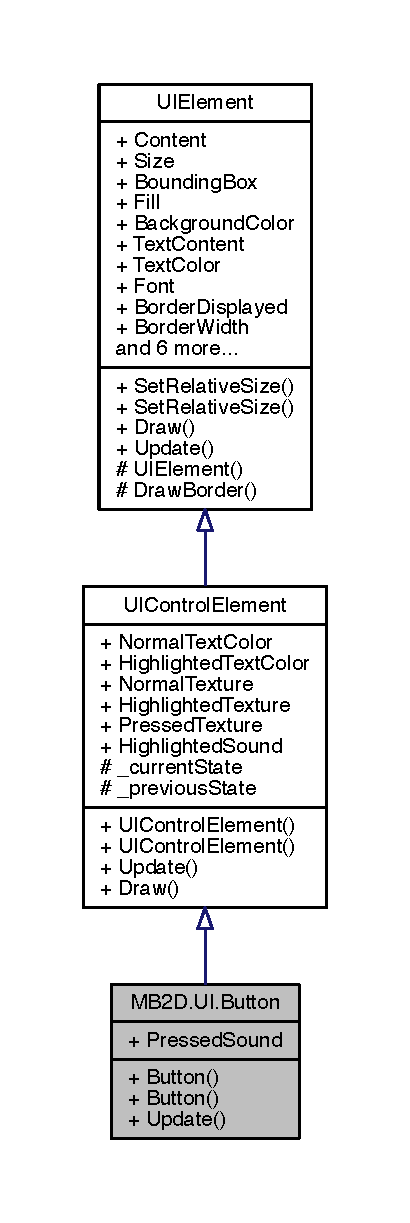
\includegraphics[height=550pt]{class_m_b2_d_1_1_u_i_1_1_button__inherit__graph}
\end{center}
\end{figure}


Collaboration diagram for M\+B2\+D.\+U\+I.\+Button\+:\nopagebreak
\begin{figure}[H]
\begin{center}
\leavevmode
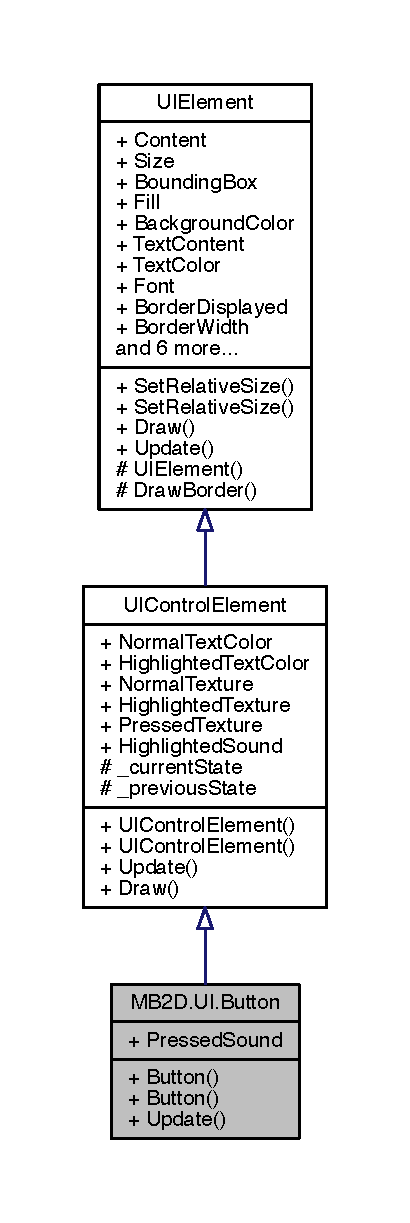
\includegraphics[height=550pt]{class_m_b2_d_1_1_u_i_1_1_button__coll__graph}
\end{center}
\end{figure}
\subsection*{Public Member Functions}
\begin{DoxyCompactItemize}
\item 
\hyperlink{class_m_b2_d_1_1_u_i_1_1_button_a30bf56105fa12c18ebffa1ba3e84cad9}{Button} (Texture2D normal, Texture2D selected, Texture2D pressed)
\begin{DoxyCompactList}\small\item\em Initializes a new instance of the T\+:\+M\+B2\+D.\+U\+I.\+Button class. \end{DoxyCompactList}\item 
\hyperlink{class_m_b2_d_1_1_u_i_1_1_button_a4d9a4339d2ebf59c059a493787790aa4}{Button} ()
\begin{DoxyCompactList}\small\item\em Initializes a new instance of the T\+:\+M\+B2\+D.\+U\+I.\+Button class with no associated textures \end{DoxyCompactList}\item 
override void \hyperlink{class_m_b2_d_1_1_u_i_1_1_button_a1686d24f172e05a1bf83fc3aa49cfab5}{Update} ()
\begin{DoxyCompactList}\small\item\em Updates the button state. \end{DoxyCompactList}\end{DoxyCompactItemize}
\subsection*{Properties}
\begin{DoxyCompactItemize}
\item 
Sound\+Effect\+Instance \hyperlink{class_m_b2_d_1_1_u_i_1_1_button_a92d0184df7962dd2aed3b8b0aa8c0d8e}{Pressed\+Sound}\hspace{0.3cm}{\ttfamily  \mbox{[}get, set\mbox{]}}
\begin{DoxyCompactList}\small\item\em Gets or sets the sound fired when transitioning to the pressed state. \end{DoxyCompactList}\end{DoxyCompactItemize}
\subsection*{Events}
\begin{DoxyCompactItemize}
\item 
Event\+Handler \hyperlink{class_m_b2_d_1_1_u_i_1_1_button_a280d1c552f9e91c7e63811bc498a4f5e}{On\+Press}
\begin{DoxyCompactList}\small\item\em Occurs when the button has been clicked or pressed. \end{DoxyCompactList}\end{DoxyCompactItemize}
\subsection*{Additional Inherited Members}


\subsection{Detailed Description}
A pressable ui element with a single On\+Press event 



\subsection{Constructor \& Destructor Documentation}
\hypertarget{class_m_b2_d_1_1_u_i_1_1_button_a30bf56105fa12c18ebffa1ba3e84cad9}{}\label{class_m_b2_d_1_1_u_i_1_1_button_a30bf56105fa12c18ebffa1ba3e84cad9} 
\index{M\+B2\+D\+::\+U\+I\+::\+Button@{M\+B2\+D\+::\+U\+I\+::\+Button}!Button@{Button}}
\index{Button@{Button}!M\+B2\+D\+::\+U\+I\+::\+Button@{M\+B2\+D\+::\+U\+I\+::\+Button}}
\subsubsection{\texorpdfstring{Button()}{Button()}\hspace{0.1cm}{\footnotesize\ttfamily [1/2]}}
{\footnotesize\ttfamily M\+B2\+D.\+U\+I.\+Button.\+Button (\begin{DoxyParamCaption}\item[{Texture2D}]{normal,  }\item[{Texture2D}]{selected,  }\item[{Texture2D}]{pressed }\end{DoxyParamCaption})\hspace{0.3cm}{\ttfamily [inline]}}



Initializes a new instance of the T\+:\+M\+B2\+D.\+U\+I.\+Button class. 


\begin{DoxyParams}{Parameters}
{\em normal} & Normal state texture\\
\hline
{\em selected} & Selected state texture.\\
\hline
{\em pressed} & Pressed state texture.\\
\hline
\end{DoxyParams}
\hypertarget{class_m_b2_d_1_1_u_i_1_1_button_a4d9a4339d2ebf59c059a493787790aa4}{}\label{class_m_b2_d_1_1_u_i_1_1_button_a4d9a4339d2ebf59c059a493787790aa4} 
\index{M\+B2\+D\+::\+U\+I\+::\+Button@{M\+B2\+D\+::\+U\+I\+::\+Button}!Button@{Button}}
\index{Button@{Button}!M\+B2\+D\+::\+U\+I\+::\+Button@{M\+B2\+D\+::\+U\+I\+::\+Button}}
\subsubsection{\texorpdfstring{Button()}{Button()}\hspace{0.1cm}{\footnotesize\ttfamily [2/2]}}
{\footnotesize\ttfamily M\+B2\+D.\+U\+I.\+Button.\+Button (\begin{DoxyParamCaption}{ }\end{DoxyParamCaption})\hspace{0.3cm}{\ttfamily [inline]}}



Initializes a new instance of the T\+:\+M\+B2\+D.\+U\+I.\+Button class with no associated textures 



\subsection{Member Function Documentation}
\hypertarget{class_m_b2_d_1_1_u_i_1_1_button_a1686d24f172e05a1bf83fc3aa49cfab5}{}\label{class_m_b2_d_1_1_u_i_1_1_button_a1686d24f172e05a1bf83fc3aa49cfab5} 
\index{M\+B2\+D\+::\+U\+I\+::\+Button@{M\+B2\+D\+::\+U\+I\+::\+Button}!Update@{Update}}
\index{Update@{Update}!M\+B2\+D\+::\+U\+I\+::\+Button@{M\+B2\+D\+::\+U\+I\+::\+Button}}
\subsubsection{\texorpdfstring{Update()}{Update()}}
{\footnotesize\ttfamily override void M\+B2\+D.\+U\+I.\+Button.\+Update (\begin{DoxyParamCaption}{ }\end{DoxyParamCaption})\hspace{0.3cm}{\ttfamily [inline]}, {\ttfamily [virtual]}}



Updates the button state. 



Implements \hyperlink{class_m_b2_d_1_1_u_i_1_1_u_i_element_aa97bcbe44f3fac8a13e2febca23b2d4d}{M\+B2\+D.\+U\+I.\+U\+I\+Element}.



\subsection{Property Documentation}
\hypertarget{class_m_b2_d_1_1_u_i_1_1_button_a92d0184df7962dd2aed3b8b0aa8c0d8e}{}\label{class_m_b2_d_1_1_u_i_1_1_button_a92d0184df7962dd2aed3b8b0aa8c0d8e} 
\index{M\+B2\+D\+::\+U\+I\+::\+Button@{M\+B2\+D\+::\+U\+I\+::\+Button}!Pressed\+Sound@{Pressed\+Sound}}
\index{Pressed\+Sound@{Pressed\+Sound}!M\+B2\+D\+::\+U\+I\+::\+Button@{M\+B2\+D\+::\+U\+I\+::\+Button}}
\subsubsection{\texorpdfstring{Pressed\+Sound}{PressedSound}}
{\footnotesize\ttfamily Sound\+Effect\+Instance M\+B2\+D.\+U\+I.\+Button.\+Pressed\+Sound\hspace{0.3cm}{\ttfamily [get]}, {\ttfamily [set]}}



Gets or sets the sound fired when transitioning to the pressed state. 

The pressed state sound.

\subsection{Event Documentation}
\hypertarget{class_m_b2_d_1_1_u_i_1_1_button_a280d1c552f9e91c7e63811bc498a4f5e}{}\label{class_m_b2_d_1_1_u_i_1_1_button_a280d1c552f9e91c7e63811bc498a4f5e} 
\index{M\+B2\+D\+::\+U\+I\+::\+Button@{M\+B2\+D\+::\+U\+I\+::\+Button}!On\+Press@{On\+Press}}
\index{On\+Press@{On\+Press}!M\+B2\+D\+::\+U\+I\+::\+Button@{M\+B2\+D\+::\+U\+I\+::\+Button}}
\subsubsection{\texorpdfstring{On\+Press}{OnPress}}
{\footnotesize\ttfamily Event\+Handler M\+B2\+D.\+U\+I.\+Button.\+On\+Press}



Occurs when the button has been clicked or pressed. 



The documentation for this class was generated from the following file\+:\begin{DoxyCompactItemize}
\item 
M\+B2\+D/src/\+U\+I/Button.\+cs\end{DoxyCompactItemize}

\hypertarget{class_m_b2_d_1_1_collectable}{}\section{M\+B2\+D.\+Collectable Class Reference}
\label{class_m_b2_d_1_1_collectable}\index{M\+B2\+D.\+Collectable@{M\+B2\+D.\+Collectable}}


Defines an object that can be contained within components and systems that operate on collectible items, such as Inventory.  




Inheritance diagram for M\+B2\+D.\+Collectable\+:\nopagebreak
\begin{figure}[H]
\begin{center}
\leavevmode
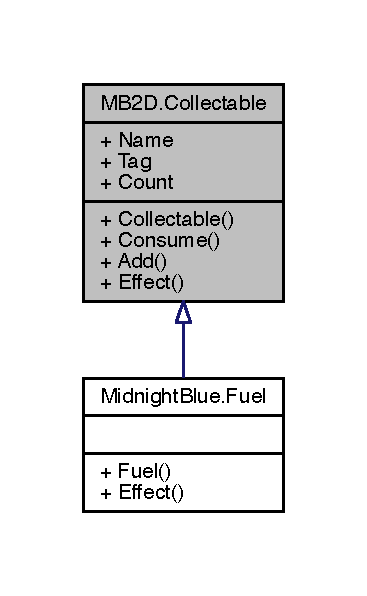
\includegraphics[width=176pt]{class_m_b2_d_1_1_collectable__inherit__graph}
\end{center}
\end{figure}


Collaboration diagram for M\+B2\+D.\+Collectable\+:\nopagebreak
\begin{figure}[H]
\begin{center}
\leavevmode
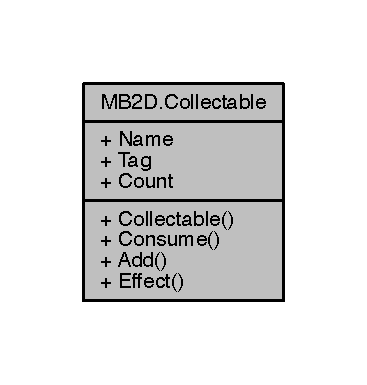
\includegraphics[width=176pt]{class_m_b2_d_1_1_collectable__coll__graph}
\end{center}
\end{figure}
\subsection*{Public Member Functions}
\begin{DoxyCompactItemize}
\item 
\hyperlink{class_m_b2_d_1_1_collectable_af635d4c8ce7035b0553f0d0bf6c8a25e}{Collectable} (string name, string tag, int initial\+Count)
\begin{DoxyCompactList}\small\item\em Initializes a new instance of the T\+:\+M\+B2\+D.\+Collectable class. \end{DoxyCompactList}\item 
void \hyperlink{class_m_b2_d_1_1_collectable_a089723a457d6a6d9249e44477f25ab9d}{Consume} (int amount=1)
\begin{DoxyCompactList}\small\item\em Consumes a number of instances of the item \end{DoxyCompactList}\item 
void \hyperlink{class_m_b2_d_1_1_collectable_a81e5756a4f1420a28674502724fc2191}{Add} (int amount=1)
\begin{DoxyCompactList}\small\item\em Adds a number of instances of this item to the container \end{DoxyCompactList}\item 
abstract void \hyperlink{class_m_b2_d_1_1_collectable_aeb2c8847eb3d5937b015f298703fd753}{Effect} (\hyperlink{class_m_b2_d_1_1_entity_component_1_1_entity}{Entity} entity)
\begin{DoxyCompactList}\small\item\em The action to enact when the item is consumed or used \end{DoxyCompactList}\end{DoxyCompactItemize}
\subsection*{Properties}
\begin{DoxyCompactItemize}
\item 
string \hyperlink{class_m_b2_d_1_1_collectable_a80d6ce8bb84f84a86ffbd58ad6237e9a}{Name}\hspace{0.3cm}{\ttfamily  \mbox{[}get\mbox{]}}
\begin{DoxyCompactList}\small\item\em Gets the name of the item. \end{DoxyCompactList}\item 
string \hyperlink{class_m_b2_d_1_1_collectable_a97f42790fdafd06634b87cd4023bc0fe}{Tag}\hspace{0.3cm}{\ttfamily  \mbox{[}get\mbox{]}}
\begin{DoxyCompactList}\small\item\em Gets the items tag. \end{DoxyCompactList}\item 
int \hyperlink{class_m_b2_d_1_1_collectable_a775364ada5d2f8095ca601657da20fc1}{Count}\hspace{0.3cm}{\ttfamily  \mbox{[}get\mbox{]}}
\begin{DoxyCompactList}\small\item\em Gets the count of available instances of the item. \end{DoxyCompactList}\end{DoxyCompactItemize}


\subsection{Detailed Description}
Defines an object that can be contained within components and systems that operate on collectible items, such as Inventory. 



\subsection{Constructor \& Destructor Documentation}
\hypertarget{class_m_b2_d_1_1_collectable_af635d4c8ce7035b0553f0d0bf6c8a25e}{}\label{class_m_b2_d_1_1_collectable_af635d4c8ce7035b0553f0d0bf6c8a25e} 
\index{M\+B2\+D\+::\+Collectable@{M\+B2\+D\+::\+Collectable}!Collectable@{Collectable}}
\index{Collectable@{Collectable}!M\+B2\+D\+::\+Collectable@{M\+B2\+D\+::\+Collectable}}
\subsubsection{\texorpdfstring{Collectable()}{Collectable()}}
{\footnotesize\ttfamily M\+B2\+D.\+Collectable.\+Collectable (\begin{DoxyParamCaption}\item[{string}]{name,  }\item[{string}]{tag,  }\item[{int}]{initial\+Count }\end{DoxyParamCaption})\hspace{0.3cm}{\ttfamily [inline]}}



Initializes a new instance of the T\+:\+M\+B2\+D.\+Collectable class. 


\begin{DoxyParams}{Parameters}
{\em name} & Name to give to the item.\\
\hline
{\em tag} & Short tag to give to the item.\\
\hline
{\em initial\+Count} & Initial count to add to the container.\\
\hline
\end{DoxyParams}


\subsection{Member Function Documentation}
\hypertarget{class_m_b2_d_1_1_collectable_a81e5756a4f1420a28674502724fc2191}{}\label{class_m_b2_d_1_1_collectable_a81e5756a4f1420a28674502724fc2191} 
\index{M\+B2\+D\+::\+Collectable@{M\+B2\+D\+::\+Collectable}!Add@{Add}}
\index{Add@{Add}!M\+B2\+D\+::\+Collectable@{M\+B2\+D\+::\+Collectable}}
\subsubsection{\texorpdfstring{Add()}{Add()}}
{\footnotesize\ttfamily void M\+B2\+D.\+Collectable.\+Add (\begin{DoxyParamCaption}\item[{int}]{amount = {\ttfamily 1} }\end{DoxyParamCaption})\hspace{0.3cm}{\ttfamily [inline]}}



Adds a number of instances of this item to the container 


\begin{DoxyParams}{Parameters}
{\em amount} & Amount to add.\\
\hline
\end{DoxyParams}
Here is the call graph for this function\+:\nopagebreak
\begin{figure}[H]
\begin{center}
\leavevmode
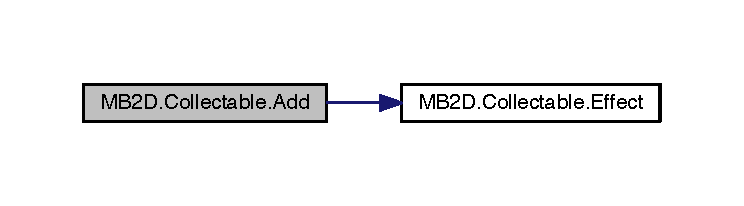
\includegraphics[width=350pt]{class_m_b2_d_1_1_collectable_a81e5756a4f1420a28674502724fc2191_cgraph}
\end{center}
\end{figure}
\hypertarget{class_m_b2_d_1_1_collectable_a089723a457d6a6d9249e44477f25ab9d}{}\label{class_m_b2_d_1_1_collectable_a089723a457d6a6d9249e44477f25ab9d} 
\index{M\+B2\+D\+::\+Collectable@{M\+B2\+D\+::\+Collectable}!Consume@{Consume}}
\index{Consume@{Consume}!M\+B2\+D\+::\+Collectable@{M\+B2\+D\+::\+Collectable}}
\subsubsection{\texorpdfstring{Consume()}{Consume()}}
{\footnotesize\ttfamily void M\+B2\+D.\+Collectable.\+Consume (\begin{DoxyParamCaption}\item[{int}]{amount = {\ttfamily 1} }\end{DoxyParamCaption})\hspace{0.3cm}{\ttfamily [inline]}}



Consumes a number of instances of the item 


\begin{DoxyParams}{Parameters}
{\em amount} & Amount to consume.\\
\hline
\end{DoxyParams}
\hypertarget{class_m_b2_d_1_1_collectable_aeb2c8847eb3d5937b015f298703fd753}{}\label{class_m_b2_d_1_1_collectable_aeb2c8847eb3d5937b015f298703fd753} 
\index{M\+B2\+D\+::\+Collectable@{M\+B2\+D\+::\+Collectable}!Effect@{Effect}}
\index{Effect@{Effect}!M\+B2\+D\+::\+Collectable@{M\+B2\+D\+::\+Collectable}}
\subsubsection{\texorpdfstring{Effect()}{Effect()}}
{\footnotesize\ttfamily abstract void M\+B2\+D.\+Collectable.\+Effect (\begin{DoxyParamCaption}\item[{\hyperlink{class_m_b2_d_1_1_entity_component_1_1_entity}{Entity}}]{entity }\end{DoxyParamCaption})\hspace{0.3cm}{\ttfamily [pure virtual]}}



The action to enact when the item is consumed or used 


\begin{DoxyParams}{Parameters}
{\em entity} & Entity to operate on.\\
\hline
\end{DoxyParams}


Implemented in \hyperlink{class_midnight_blue_1_1_fuel_a9ab52c79211ec8cdcc9389f772615ac0}{Midnight\+Blue.\+Fuel}.

Here is the caller graph for this function\+:\nopagebreak
\begin{figure}[H]
\begin{center}
\leavevmode
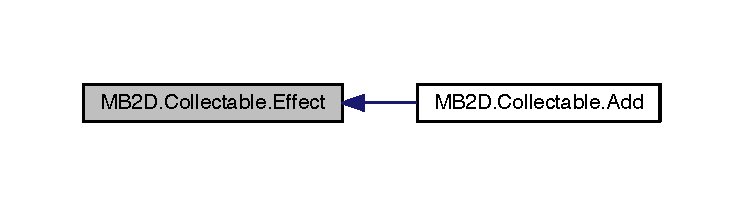
\includegraphics[width=350pt]{class_m_b2_d_1_1_collectable_aeb2c8847eb3d5937b015f298703fd753_icgraph}
\end{center}
\end{figure}


\subsection{Property Documentation}
\hypertarget{class_m_b2_d_1_1_collectable_a775364ada5d2f8095ca601657da20fc1}{}\label{class_m_b2_d_1_1_collectable_a775364ada5d2f8095ca601657da20fc1} 
\index{M\+B2\+D\+::\+Collectable@{M\+B2\+D\+::\+Collectable}!Count@{Count}}
\index{Count@{Count}!M\+B2\+D\+::\+Collectable@{M\+B2\+D\+::\+Collectable}}
\subsubsection{\texorpdfstring{Count}{Count}}
{\footnotesize\ttfamily int M\+B2\+D.\+Collectable.\+Count\hspace{0.3cm}{\ttfamily [get]}}



Gets the count of available instances of the item. 

The count.\hypertarget{class_m_b2_d_1_1_collectable_a80d6ce8bb84f84a86ffbd58ad6237e9a}{}\label{class_m_b2_d_1_1_collectable_a80d6ce8bb84f84a86ffbd58ad6237e9a} 
\index{M\+B2\+D\+::\+Collectable@{M\+B2\+D\+::\+Collectable}!Name@{Name}}
\index{Name@{Name}!M\+B2\+D\+::\+Collectable@{M\+B2\+D\+::\+Collectable}}
\subsubsection{\texorpdfstring{Name}{Name}}
{\footnotesize\ttfamily string M\+B2\+D.\+Collectable.\+Name\hspace{0.3cm}{\ttfamily [get]}}



Gets the name of the item. 

The name.\hypertarget{class_m_b2_d_1_1_collectable_a97f42790fdafd06634b87cd4023bc0fe}{}\label{class_m_b2_d_1_1_collectable_a97f42790fdafd06634b87cd4023bc0fe} 
\index{M\+B2\+D\+::\+Collectable@{M\+B2\+D\+::\+Collectable}!Tag@{Tag}}
\index{Tag@{Tag}!M\+B2\+D\+::\+Collectable@{M\+B2\+D\+::\+Collectable}}
\subsubsection{\texorpdfstring{Tag}{Tag}}
{\footnotesize\ttfamily string M\+B2\+D.\+Collectable.\+Tag\hspace{0.3cm}{\ttfamily [get]}}



Gets the items tag. 

The tag.

The documentation for this class was generated from the following file\+:\begin{DoxyCompactItemize}
\item 
M\+B2\+D/src/\+Inventory/Collectable.\+cs\end{DoxyCompactItemize}

\hypertarget{class_m_b2_d_1_1_collision_1_1_collision_cell}{}\section{M\+B2\+D.\+Collision.\+Collision\+Cell Class Reference}
\label{class_m_b2_d_1_1_collision_1_1_collision_cell}\index{M\+B2\+D.\+Collision.\+Collision\+Cell@{M\+B2\+D.\+Collision.\+Collision\+Cell}}


A cell used in a collision map to hold a linked list of all its contained entities  




Collaboration diagram for M\+B2\+D.\+Collision.\+Collision\+Cell\+:\nopagebreak
\begin{figure}[H]
\begin{center}
\leavevmode
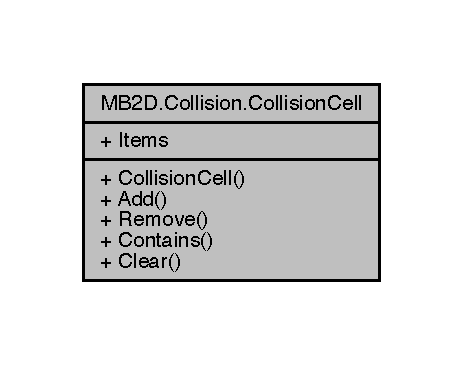
\includegraphics[width=222pt]{class_m_b2_d_1_1_collision_1_1_collision_cell__coll__graph}
\end{center}
\end{figure}
\subsection*{Public Member Functions}
\begin{DoxyCompactItemize}
\item 
\hyperlink{class_m_b2_d_1_1_collision_1_1_collision_cell_a2eefdbb1f60eb35c38c45b4a0f4d939d}{Collision\+Cell} ()
\begin{DoxyCompactList}\small\item\em Initializes a new instance of the T\+:\+M\+B2\+D.\+Collision.\+Collision\+Cell class. \end{DoxyCompactList}\item 
void \hyperlink{class_m_b2_d_1_1_collision_1_1_collision_cell_a4fc338d7dbfd7418f5493424c5937213}{Add} (\hyperlink{class_m_b2_d_1_1_entity_component_1_1_entity}{Entity} entity)
\begin{DoxyCompactList}\small\item\em Adds an entity to the cell \end{DoxyCompactList}\item 
void \hyperlink{class_m_b2_d_1_1_collision_1_1_collision_cell_a064f540f907885b4224119308cbf1761}{Remove} (\hyperlink{class_m_b2_d_1_1_entity_component_1_1_entity}{Entity} entity)
\begin{DoxyCompactList}\small\item\em Removes a specific entity from the cell \end{DoxyCompactList}\item 
bool \hyperlink{class_m_b2_d_1_1_collision_1_1_collision_cell_aa4be244387541ee24d88da80331b3438}{Contains} (\hyperlink{class_m_b2_d_1_1_entity_component_1_1_entity}{Entity} entity)
\begin{DoxyCompactList}\small\item\em Checks if the entity is inside the cell already \end{DoxyCompactList}\item 
void \hyperlink{class_m_b2_d_1_1_collision_1_1_collision_cell_ae4ff144f6c768003d8be46e17e130646}{Clear} ()
\begin{DoxyCompactList}\small\item\em Clear the cell of all entities. \end{DoxyCompactList}\end{DoxyCompactItemize}
\subsection*{Properties}
\begin{DoxyCompactItemize}
\item 
Linked\+List$<$ \hyperlink{class_m_b2_d_1_1_entity_component_1_1_entity}{Entity} $>$ \hyperlink{class_m_b2_d_1_1_collision_1_1_collision_cell_ab893dad8ce4d09c5ab38a5da93145755}{Items}\hspace{0.3cm}{\ttfamily  \mbox{[}get\mbox{]}}
\begin{DoxyCompactList}\small\item\em Gets the list of this cells entities \end{DoxyCompactList}\end{DoxyCompactItemize}


\subsection{Detailed Description}
A cell used in a collision map to hold a linked list of all its contained entities 



\subsection{Constructor \& Destructor Documentation}
\hypertarget{class_m_b2_d_1_1_collision_1_1_collision_cell_a2eefdbb1f60eb35c38c45b4a0f4d939d}{}\label{class_m_b2_d_1_1_collision_1_1_collision_cell_a2eefdbb1f60eb35c38c45b4a0f4d939d} 
\index{M\+B2\+D\+::\+Collision\+::\+Collision\+Cell@{M\+B2\+D\+::\+Collision\+::\+Collision\+Cell}!Collision\+Cell@{Collision\+Cell}}
\index{Collision\+Cell@{Collision\+Cell}!M\+B2\+D\+::\+Collision\+::\+Collision\+Cell@{M\+B2\+D\+::\+Collision\+::\+Collision\+Cell}}
\subsubsection{\texorpdfstring{Collision\+Cell()}{CollisionCell()}}
{\footnotesize\ttfamily M\+B2\+D.\+Collision.\+Collision\+Cell.\+Collision\+Cell (\begin{DoxyParamCaption}{ }\end{DoxyParamCaption})\hspace{0.3cm}{\ttfamily [inline]}}



Initializes a new instance of the T\+:\+M\+B2\+D.\+Collision.\+Collision\+Cell class. 



\subsection{Member Function Documentation}
\hypertarget{class_m_b2_d_1_1_collision_1_1_collision_cell_a4fc338d7dbfd7418f5493424c5937213}{}\label{class_m_b2_d_1_1_collision_1_1_collision_cell_a4fc338d7dbfd7418f5493424c5937213} 
\index{M\+B2\+D\+::\+Collision\+::\+Collision\+Cell@{M\+B2\+D\+::\+Collision\+::\+Collision\+Cell}!Add@{Add}}
\index{Add@{Add}!M\+B2\+D\+::\+Collision\+::\+Collision\+Cell@{M\+B2\+D\+::\+Collision\+::\+Collision\+Cell}}
\subsubsection{\texorpdfstring{Add()}{Add()}}
{\footnotesize\ttfamily void M\+B2\+D.\+Collision.\+Collision\+Cell.\+Add (\begin{DoxyParamCaption}\item[{\hyperlink{class_m_b2_d_1_1_entity_component_1_1_entity}{Entity}}]{entity }\end{DoxyParamCaption})\hspace{0.3cm}{\ttfamily [inline]}}



Adds an entity to the cell 


\begin{DoxyParams}{Parameters}
{\em entity} & Entity to add.\\
\hline
\end{DoxyParams}
Here is the caller graph for this function\+:\nopagebreak
\begin{figure}[H]
\begin{center}
\leavevmode
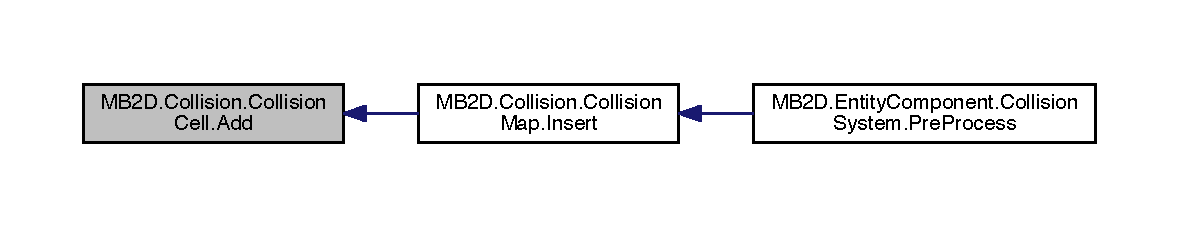
\includegraphics[width=350pt]{class_m_b2_d_1_1_collision_1_1_collision_cell_a4fc338d7dbfd7418f5493424c5937213_icgraph}
\end{center}
\end{figure}
\hypertarget{class_m_b2_d_1_1_collision_1_1_collision_cell_ae4ff144f6c768003d8be46e17e130646}{}\label{class_m_b2_d_1_1_collision_1_1_collision_cell_ae4ff144f6c768003d8be46e17e130646} 
\index{M\+B2\+D\+::\+Collision\+::\+Collision\+Cell@{M\+B2\+D\+::\+Collision\+::\+Collision\+Cell}!Clear@{Clear}}
\index{Clear@{Clear}!M\+B2\+D\+::\+Collision\+::\+Collision\+Cell@{M\+B2\+D\+::\+Collision\+::\+Collision\+Cell}}
\subsubsection{\texorpdfstring{Clear()}{Clear()}}
{\footnotesize\ttfamily void M\+B2\+D.\+Collision.\+Collision\+Cell.\+Clear (\begin{DoxyParamCaption}{ }\end{DoxyParamCaption})\hspace{0.3cm}{\ttfamily [inline]}}



Clear the cell of all entities. 

\hypertarget{class_m_b2_d_1_1_collision_1_1_collision_cell_aa4be244387541ee24d88da80331b3438}{}\label{class_m_b2_d_1_1_collision_1_1_collision_cell_aa4be244387541ee24d88da80331b3438} 
\index{M\+B2\+D\+::\+Collision\+::\+Collision\+Cell@{M\+B2\+D\+::\+Collision\+::\+Collision\+Cell}!Contains@{Contains}}
\index{Contains@{Contains}!M\+B2\+D\+::\+Collision\+::\+Collision\+Cell@{M\+B2\+D\+::\+Collision\+::\+Collision\+Cell}}
\subsubsection{\texorpdfstring{Contains()}{Contains()}}
{\footnotesize\ttfamily bool M\+B2\+D.\+Collision.\+Collision\+Cell.\+Contains (\begin{DoxyParamCaption}\item[{\hyperlink{class_m_b2_d_1_1_entity_component_1_1_entity}{Entity}}]{entity }\end{DoxyParamCaption})\hspace{0.3cm}{\ttfamily [inline]}}



Checks if the entity is inside the cell already 


\begin{DoxyParams}{Parameters}
{\em entity} & Entity.\\
\hline
\end{DoxyParams}
\hypertarget{class_m_b2_d_1_1_collision_1_1_collision_cell_a064f540f907885b4224119308cbf1761}{}\label{class_m_b2_d_1_1_collision_1_1_collision_cell_a064f540f907885b4224119308cbf1761} 
\index{M\+B2\+D\+::\+Collision\+::\+Collision\+Cell@{M\+B2\+D\+::\+Collision\+::\+Collision\+Cell}!Remove@{Remove}}
\index{Remove@{Remove}!M\+B2\+D\+::\+Collision\+::\+Collision\+Cell@{M\+B2\+D\+::\+Collision\+::\+Collision\+Cell}}
\subsubsection{\texorpdfstring{Remove()}{Remove()}}
{\footnotesize\ttfamily void M\+B2\+D.\+Collision.\+Collision\+Cell.\+Remove (\begin{DoxyParamCaption}\item[{\hyperlink{class_m_b2_d_1_1_entity_component_1_1_entity}{Entity}}]{entity }\end{DoxyParamCaption})\hspace{0.3cm}{\ttfamily [inline]}}



Removes a specific entity from the cell 


\begin{DoxyParams}{Parameters}
{\em entity} & Entity to remove.\\
\hline
\end{DoxyParams}


\subsection{Property Documentation}
\hypertarget{class_m_b2_d_1_1_collision_1_1_collision_cell_ab893dad8ce4d09c5ab38a5da93145755}{}\label{class_m_b2_d_1_1_collision_1_1_collision_cell_ab893dad8ce4d09c5ab38a5da93145755} 
\index{M\+B2\+D\+::\+Collision\+::\+Collision\+Cell@{M\+B2\+D\+::\+Collision\+::\+Collision\+Cell}!Items@{Items}}
\index{Items@{Items}!M\+B2\+D\+::\+Collision\+::\+Collision\+Cell@{M\+B2\+D\+::\+Collision\+::\+Collision\+Cell}}
\subsubsection{\texorpdfstring{Items}{Items}}
{\footnotesize\ttfamily Linked\+List$<$\hyperlink{class_m_b2_d_1_1_entity_component_1_1_entity}{Entity}$>$ M\+B2\+D.\+Collision.\+Collision\+Cell.\+Items\hspace{0.3cm}{\ttfamily [get]}}



Gets the list of this cells entities 

The entities.

The documentation for this class was generated from the following file\+:\begin{DoxyCompactItemize}
\item 
M\+B2\+D/src/\+Collision/Collision\+Cell.\+cs\end{DoxyCompactItemize}

\hypertarget{class_m_b2_d_1_1_entity_component_1_1_collision_component}{}\section{M\+B2\+D.\+Entity\+Component.\+Collision\+Component Class Reference}
\label{class_m_b2_d_1_1_entity_component_1_1_collision_component}\index{M\+B2\+D.\+Entity\+Component.\+Collision\+Component@{M\+B2\+D.\+Entity\+Component.\+Collision\+Component}}


Used for running collision detection on an \hyperlink{class_m_b2_d_1_1_entity_component_1_1_entity}{Entity}  




Inheritance diagram for M\+B2\+D.\+Entity\+Component.\+Collision\+Component\+:
\nopagebreak
\begin{figure}[H]
\begin{center}
\leavevmode
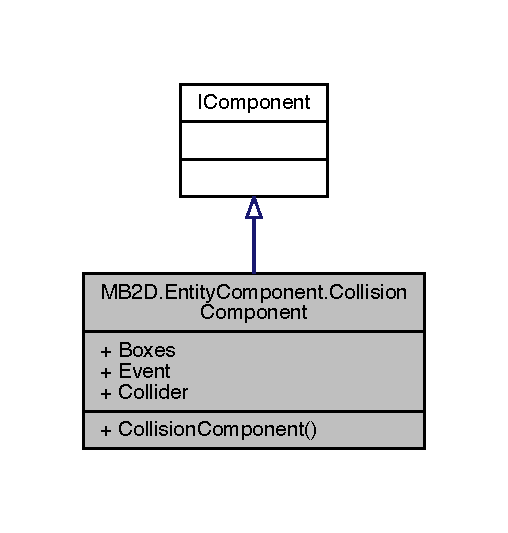
\includegraphics[width=244pt]{class_m_b2_d_1_1_entity_component_1_1_collision_component__inherit__graph}
\end{center}
\end{figure}


Collaboration diagram for M\+B2\+D.\+Entity\+Component.\+Collision\+Component\+:
\nopagebreak
\begin{figure}[H]
\begin{center}
\leavevmode
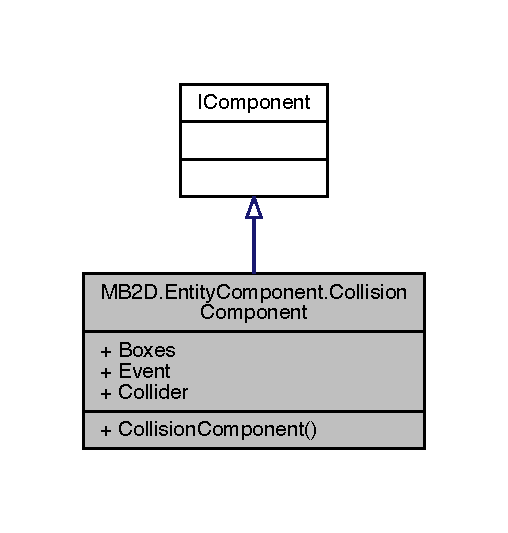
\includegraphics[width=244pt]{class_m_b2_d_1_1_entity_component_1_1_collision_component__coll__graph}
\end{center}
\end{figure}
\subsection*{Public Member Functions}
\begin{DoxyCompactItemize}
\item 
\hyperlink{class_m_b2_d_1_1_entity_component_1_1_collision_component_a6367fc81a9baf226bdd98cdc5814f5ac}{Collision\+Component} (params RectangleF\mbox{[}$\,$\mbox{]} boxes)
\begin{DoxyCompactList}\small\item\em Initializes a new instance of the T\+:\+M\+B2\+D.\+Entity\+Component.\+Collision\+Component class with an array of its associated A\+A\+BB\textquotesingle{}s \end{DoxyCompactList}\end{DoxyCompactItemize}
\subsection*{Properties}
\begin{DoxyCompactItemize}
\item 
List$<$ RectangleF $>$ \hyperlink{class_m_b2_d_1_1_entity_component_1_1_collision_component_a1cc63c601df7e30ce5b63e50b487dc9e}{Boxes}\hspace{0.3cm}{\ttfamily  \mbox{[}get, set\mbox{]}}
\begin{DoxyCompactList}\small\item\em Gets or sets the list of bounding boxes used for collision detection. \end{DoxyCompactList}\item 
bool \hyperlink{class_m_b2_d_1_1_entity_component_1_1_collision_component_ad393ea9f0115ee346e469e5c335da26d}{Event}\hspace{0.3cm}{\ttfamily  \mbox{[}get, set\mbox{]}}
\begin{DoxyCompactList}\small\item\em Gets or sets a value indicating whether this T\+:\+M\+B2\+D.\+Entity\+Component.\+Collision\+Component has had a collision event this frame. \end{DoxyCompactList}\item 
\hyperlink{class_m_b2_d_1_1_entity_component_1_1_entity}{Entity} \hyperlink{class_m_b2_d_1_1_entity_component_1_1_collision_component_aac8e61b6e669a4451fb2e8859827b47a}{Collider}\hspace{0.3cm}{\ttfamily  \mbox{[}get, set\mbox{]}}
\begin{DoxyCompactList}\small\item\em Gets or sets the collider entity associated with the collision event. \end{DoxyCompactList}\end{DoxyCompactItemize}


\subsection{Detailed Description}
Used for running collision detection on an \hyperlink{class_m_b2_d_1_1_entity_component_1_1_entity}{Entity} 



\subsection{Constructor \& Destructor Documentation}
\hypertarget{class_m_b2_d_1_1_entity_component_1_1_collision_component_a6367fc81a9baf226bdd98cdc5814f5ac}{}\label{class_m_b2_d_1_1_entity_component_1_1_collision_component_a6367fc81a9baf226bdd98cdc5814f5ac} 
\index{M\+B2\+D\+::\+Entity\+Component\+::\+Collision\+Component@{M\+B2\+D\+::\+Entity\+Component\+::\+Collision\+Component}!Collision\+Component@{Collision\+Component}}
\index{Collision\+Component@{Collision\+Component}!M\+B2\+D\+::\+Entity\+Component\+::\+Collision\+Component@{M\+B2\+D\+::\+Entity\+Component\+::\+Collision\+Component}}
\subsubsection{\texorpdfstring{Collision\+Component()}{CollisionComponent()}}
{\footnotesize\ttfamily M\+B2\+D.\+Entity\+Component.\+Collision\+Component.\+Collision\+Component (\begin{DoxyParamCaption}\item[{params RectangleF \mbox{[}$\,$\mbox{]}}]{boxes }\end{DoxyParamCaption})\hspace{0.3cm}{\ttfamily [inline]}}



Initializes a new instance of the T\+:\+M\+B2\+D.\+Entity\+Component.\+Collision\+Component class with an array of its associated A\+A\+BB\textquotesingle{}s 


\begin{DoxyParams}{Parameters}
{\em boxes} & The bounding boxes used for detecting collisions.\\
\hline
\end{DoxyParams}


\subsection{Property Documentation}
\hypertarget{class_m_b2_d_1_1_entity_component_1_1_collision_component_a1cc63c601df7e30ce5b63e50b487dc9e}{}\label{class_m_b2_d_1_1_entity_component_1_1_collision_component_a1cc63c601df7e30ce5b63e50b487dc9e} 
\index{M\+B2\+D\+::\+Entity\+Component\+::\+Collision\+Component@{M\+B2\+D\+::\+Entity\+Component\+::\+Collision\+Component}!Boxes@{Boxes}}
\index{Boxes@{Boxes}!M\+B2\+D\+::\+Entity\+Component\+::\+Collision\+Component@{M\+B2\+D\+::\+Entity\+Component\+::\+Collision\+Component}}
\subsubsection{\texorpdfstring{Boxes}{Boxes}}
{\footnotesize\ttfamily List$<$RectangleF$>$ M\+B2\+D.\+Entity\+Component.\+Collision\+Component.\+Boxes\hspace{0.3cm}{\ttfamily [get]}, {\ttfamily [set]}}



Gets or sets the list of bounding boxes used for collision detection. 

The boxes.\hypertarget{class_m_b2_d_1_1_entity_component_1_1_collision_component_aac8e61b6e669a4451fb2e8859827b47a}{}\label{class_m_b2_d_1_1_entity_component_1_1_collision_component_aac8e61b6e669a4451fb2e8859827b47a} 
\index{M\+B2\+D\+::\+Entity\+Component\+::\+Collision\+Component@{M\+B2\+D\+::\+Entity\+Component\+::\+Collision\+Component}!Collider@{Collider}}
\index{Collider@{Collider}!M\+B2\+D\+::\+Entity\+Component\+::\+Collision\+Component@{M\+B2\+D\+::\+Entity\+Component\+::\+Collision\+Component}}
\subsubsection{\texorpdfstring{Collider}{Collider}}
{\footnotesize\ttfamily \hyperlink{class_m_b2_d_1_1_entity_component_1_1_entity}{Entity} M\+B2\+D.\+Entity\+Component.\+Collision\+Component.\+Collider\hspace{0.3cm}{\ttfamily [get]}, {\ttfamily [set]}}



Gets or sets the collider entity associated with the collision event. 

The collider.\hypertarget{class_m_b2_d_1_1_entity_component_1_1_collision_component_ad393ea9f0115ee346e469e5c335da26d}{}\label{class_m_b2_d_1_1_entity_component_1_1_collision_component_ad393ea9f0115ee346e469e5c335da26d} 
\index{M\+B2\+D\+::\+Entity\+Component\+::\+Collision\+Component@{M\+B2\+D\+::\+Entity\+Component\+::\+Collision\+Component}!Event@{Event}}
\index{Event@{Event}!M\+B2\+D\+::\+Entity\+Component\+::\+Collision\+Component@{M\+B2\+D\+::\+Entity\+Component\+::\+Collision\+Component}}
\subsubsection{\texorpdfstring{Event}{Event}}
{\footnotesize\ttfamily bool M\+B2\+D.\+Entity\+Component.\+Collision\+Component.\+Event\hspace{0.3cm}{\ttfamily [get]}, {\ttfamily [set]}}



Gets or sets a value indicating whether this T\+:\+M\+B2\+D.\+Entity\+Component.\+Collision\+Component has had a collision event this frame. 

{\ttfamily true} if an event ocurred; otherwise, {\ttfamily false}.

The documentation for this class was generated from the following file\+:\begin{DoxyCompactItemize}
\item 
M\+B2\+D/src/\+Entity\+Component/\+Components/Collision\+Component.\+cs\end{DoxyCompactItemize}

\hypertarget{class_m_b2_d_1_1_collision_1_1_collision_map}{}\subsection{M\+B2\+D.\+Collision.\+Collision\+Map Class Reference}
\label{class_m_b2_d_1_1_collision_1_1_collision_map}\index{M\+B2\+D.\+Collision.\+Collision\+Map@{M\+B2\+D.\+Collision.\+Collision\+Map}}


A 2D Grid that represents a particular space in the game world to check for collisions. Uses spatial indexing to determine where an entity will be located at any given time. For best results, the cellsize and overall size of the map should be tweaked for each individual game screen and environment.  




Collaboration diagram for M\+B2\+D.\+Collision.\+Collision\+Map\+:
\nopagebreak
\begin{figure}[H]
\begin{center}
\leavevmode
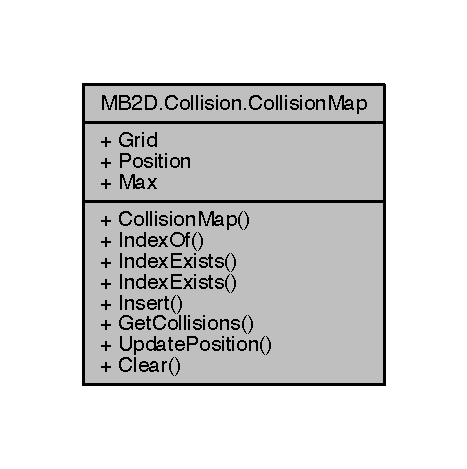
\includegraphics[width=224pt]{class_m_b2_d_1_1_collision_1_1_collision_map__coll__graph}
\end{center}
\end{figure}
\subsubsection*{Public Member Functions}
\begin{DoxyCompactItemize}
\item 
\hyperlink{class_m_b2_d_1_1_collision_1_1_collision_map_a715fbf658eed15c6f54a38a9bbb0cc82}{Collision\+Map} (int x\+Min, int x\+Max, int y\+Min, int y\+Max, int cell\+Size)
\begin{DoxyCompactList}\small\item\em Initializes a new instance of the T\+:\+M\+B2\+D.\+Collision.\+Collision\+Map class. \end{DoxyCompactList}\item 
Point \hyperlink{class_m_b2_d_1_1_collision_1_1_collision_map_a738f7b15771993a037044aace6a6e09b}{Index\+Of} (Point position)
\begin{DoxyCompactList}\small\item\em Indexes a world-\/based coordinate into the collision grid \end{DoxyCompactList}\item 
bool \hyperlink{class_m_b2_d_1_1_collision_1_1_collision_map_adb3b318fb729bd02cda21a450e504465}{Index\+Exists} (int x, int y)
\begin{DoxyCompactList}\small\item\em Checks if a particular index exists in the grid \end{DoxyCompactList}\item 
bool \hyperlink{class_m_b2_d_1_1_collision_1_1_collision_map_aa90ce934e081513f78aceacab50f27da}{Index\+Exists} (Point index)
\begin{DoxyCompactList}\small\item\em Checks if a particular index exists in the grid \end{DoxyCompactList}\item 
void \hyperlink{class_m_b2_d_1_1_collision_1_1_collision_map_a7d53571c049d50d62e6132413fe712e3}{Insert} (\hyperlink{class_m_b2_d_1_1_entity_component_1_1_entity}{Entity} entity, \hyperlink{class_m_b2_d_1_1_entity_component_1_1_collision_component}{Collision\+Component} collision)
\begin{DoxyCompactList}\small\item\em Inserts an entity and its associated collision component into the grid \end{DoxyCompactList}\item 
List$<$ \hyperlink{class_m_b2_d_1_1_entity_component_1_1_entity}{Entity} $>$ \hyperlink{class_m_b2_d_1_1_collision_1_1_collision_map_acbc6d9d9bb85342cf8f07c22f6947b27}{Get\+Collisions} (\hyperlink{class_m_b2_d_1_1_entity_component_1_1_entity}{Entity} entity, \hyperlink{class_m_b2_d_1_1_entity_component_1_1_collision_component}{Collision\+Component} collision)
\begin{DoxyCompactList}\small\item\em Gets a list of all entities located in the same cell/s as a specific single entity \end{DoxyCompactList}\item 
void \hyperlink{class_m_b2_d_1_1_collision_1_1_collision_map_a8f34c934947ce25d7de681fc07f14e09}{Update\+Position} (int x, int y)
\begin{DoxyCompactList}\small\item\em Updates the position of the collision grid. \end{DoxyCompactList}\item 
void \hyperlink{class_m_b2_d_1_1_collision_1_1_collision_map_ac7eeef6db2deadf738ea40ff939759ff}{Clear} ()
\begin{DoxyCompactList}\small\item\em Clears all non-\/empty cells of the grid from their entities \end{DoxyCompactList}\end{DoxyCompactItemize}
\subsubsection*{Properties}
\begin{DoxyCompactItemize}
\item 
\hyperlink{class_m_b2_d_1_1_geometry_1_1_grid}{Grid} \hyperlink{class_m_b2_d_1_1_collision_1_1_collision_map_aacfa35801f16fad4ea0d128edf522095}{Grid}\hspace{0.3cm}{\ttfamily  \mbox{[}get\mbox{]}}
\begin{DoxyCompactList}\small\item\em Gets the geometric representation of the grid \end{DoxyCompactList}\item 
Vector2 \hyperlink{class_m_b2_d_1_1_collision_1_1_collision_map_a0d069be50f64db9f09d488dc2642ee48}{Position}\hspace{0.3cm}{\ttfamily  \mbox{[}get\mbox{]}}
\begin{DoxyCompactList}\small\item\em Gets the current position of the grid. \end{DoxyCompactList}\item 
Vector2 \hyperlink{class_m_b2_d_1_1_collision_1_1_collision_map_a707dab6ca65cfe316c248976a0d750f6}{Max}\hspace{0.3cm}{\ttfamily  \mbox{[}get\mbox{]}}
\begin{DoxyCompactList}\small\item\em Gets the upper bounds of the x and y coordinates in the grid \end{DoxyCompactList}\end{DoxyCompactItemize}


\subsubsection{Detailed Description}
A 2D Grid that represents a particular space in the game world to check for collisions. Uses spatial indexing to determine where an entity will be located at any given time. For best results, the cellsize and overall size of the map should be tweaked for each individual game screen and environment. 



\subsubsection{Constructor \& Destructor Documentation}
\hypertarget{class_m_b2_d_1_1_collision_1_1_collision_map_a715fbf658eed15c6f54a38a9bbb0cc82}{}\label{class_m_b2_d_1_1_collision_1_1_collision_map_a715fbf658eed15c6f54a38a9bbb0cc82} 
\index{M\+B2\+D\+::\+Collision\+::\+Collision\+Map@{M\+B2\+D\+::\+Collision\+::\+Collision\+Map}!Collision\+Map@{Collision\+Map}}
\index{Collision\+Map@{Collision\+Map}!M\+B2\+D\+::\+Collision\+::\+Collision\+Map@{M\+B2\+D\+::\+Collision\+::\+Collision\+Map}}
\paragraph{\texorpdfstring{Collision\+Map()}{CollisionMap()}}
{\footnotesize\ttfamily M\+B2\+D.\+Collision.\+Collision\+Map.\+Collision\+Map (\begin{DoxyParamCaption}\item[{int}]{x\+Min,  }\item[{int}]{x\+Max,  }\item[{int}]{y\+Min,  }\item[{int}]{y\+Max,  }\item[{int}]{cell\+Size }\end{DoxyParamCaption})\hspace{0.3cm}{\ttfamily [inline]}}



Initializes a new instance of the T\+:\+M\+B2\+D.\+Collision.\+Collision\+Map class. 


\begin{DoxyParams}{Parameters}
{\em x\+Min} & The grids left most x coordinate.\\
\hline
{\em x\+Max} & Right most x coordinae.\\
\hline
{\em y\+Min} & Top most y coordinate.\\
\hline
{\em y\+Max} & Bottom most y coordinate.\\
\hline
{\em cell\+Size} & The size of each cell in the grid.\\
\hline
\end{DoxyParams}


\subsubsection{Member Function Documentation}
\hypertarget{class_m_b2_d_1_1_collision_1_1_collision_map_ac7eeef6db2deadf738ea40ff939759ff}{}\label{class_m_b2_d_1_1_collision_1_1_collision_map_ac7eeef6db2deadf738ea40ff939759ff} 
\index{M\+B2\+D\+::\+Collision\+::\+Collision\+Map@{M\+B2\+D\+::\+Collision\+::\+Collision\+Map}!Clear@{Clear}}
\index{Clear@{Clear}!M\+B2\+D\+::\+Collision\+::\+Collision\+Map@{M\+B2\+D\+::\+Collision\+::\+Collision\+Map}}
\paragraph{\texorpdfstring{Clear()}{Clear()}}
{\footnotesize\ttfamily void M\+B2\+D.\+Collision.\+Collision\+Map.\+Clear (\begin{DoxyParamCaption}{ }\end{DoxyParamCaption})\hspace{0.3cm}{\ttfamily [inline]}}



Clears all non-\/empty cells of the grid from their entities 

Here is the caller graph for this function\+:
\nopagebreak
\begin{figure}[H]
\begin{center}
\leavevmode
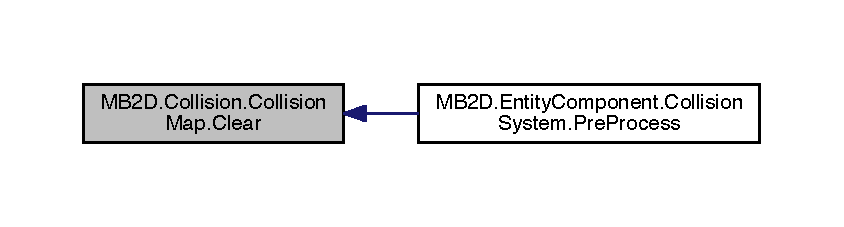
\includegraphics[width=350pt]{class_m_b2_d_1_1_collision_1_1_collision_map_ac7eeef6db2deadf738ea40ff939759ff_icgraph}
\end{center}
\end{figure}
\hypertarget{class_m_b2_d_1_1_collision_1_1_collision_map_acbc6d9d9bb85342cf8f07c22f6947b27}{}\label{class_m_b2_d_1_1_collision_1_1_collision_map_acbc6d9d9bb85342cf8f07c22f6947b27} 
\index{M\+B2\+D\+::\+Collision\+::\+Collision\+Map@{M\+B2\+D\+::\+Collision\+::\+Collision\+Map}!Get\+Collisions@{Get\+Collisions}}
\index{Get\+Collisions@{Get\+Collisions}!M\+B2\+D\+::\+Collision\+::\+Collision\+Map@{M\+B2\+D\+::\+Collision\+::\+Collision\+Map}}
\paragraph{\texorpdfstring{Get\+Collisions()}{GetCollisions()}}
{\footnotesize\ttfamily List$<$\hyperlink{class_m_b2_d_1_1_entity_component_1_1_entity}{Entity}$>$ M\+B2\+D.\+Collision.\+Collision\+Map.\+Get\+Collisions (\begin{DoxyParamCaption}\item[{\hyperlink{class_m_b2_d_1_1_entity_component_1_1_entity}{Entity}}]{entity,  }\item[{\hyperlink{class_m_b2_d_1_1_entity_component_1_1_collision_component}{Collision\+Component}}]{collision }\end{DoxyParamCaption})\hspace{0.3cm}{\ttfamily [inline]}}



Gets a list of all entities located in the same cell/s as a specific single entity 

\begin{DoxyReturn}{Returns}
The entities neighbours.
\end{DoxyReturn}

\begin{DoxyParams}{Parameters}
{\em entity} & Entity to get collisions for.\\
\hline
{\em collision} & \hyperlink{namespace_m_b2_d_1_1_collision}{Collision} component to use in checking.\\
\hline
\end{DoxyParams}
Here is the caller graph for this function\+:
\nopagebreak
\begin{figure}[H]
\begin{center}
\leavevmode
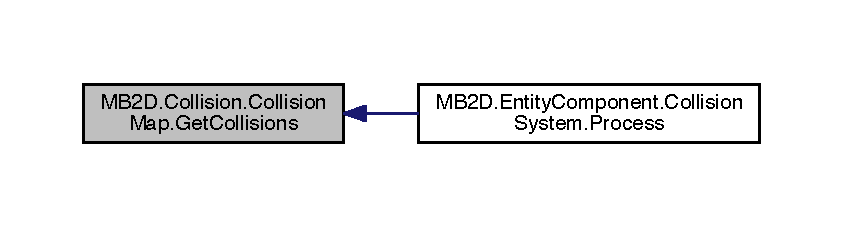
\includegraphics[width=350pt]{class_m_b2_d_1_1_collision_1_1_collision_map_acbc6d9d9bb85342cf8f07c22f6947b27_icgraph}
\end{center}
\end{figure}
\hypertarget{class_m_b2_d_1_1_collision_1_1_collision_map_adb3b318fb729bd02cda21a450e504465}{}\label{class_m_b2_d_1_1_collision_1_1_collision_map_adb3b318fb729bd02cda21a450e504465} 
\index{M\+B2\+D\+::\+Collision\+::\+Collision\+Map@{M\+B2\+D\+::\+Collision\+::\+Collision\+Map}!Index\+Exists@{Index\+Exists}}
\index{Index\+Exists@{Index\+Exists}!M\+B2\+D\+::\+Collision\+::\+Collision\+Map@{M\+B2\+D\+::\+Collision\+::\+Collision\+Map}}
\paragraph{\texorpdfstring{Index\+Exists()}{IndexExists()}\hspace{0.1cm}{\footnotesize\ttfamily [1/2]}}
{\footnotesize\ttfamily bool M\+B2\+D.\+Collision.\+Collision\+Map.\+Index\+Exists (\begin{DoxyParamCaption}\item[{int}]{x,  }\item[{int}]{y }\end{DoxyParamCaption})\hspace{0.3cm}{\ttfamily [inline]}}



Checks if a particular index exists in the grid 

\begin{DoxyReturn}{Returns}
{\ttfamily true}, if index exists, {\ttfamily false} otherwise.
\end{DoxyReturn}

\begin{DoxyParams}{Parameters}
{\em x} & The x coordinate.\\
\hline
{\em y} & The y coordinate.\\
\hline
\end{DoxyParams}
\hypertarget{class_m_b2_d_1_1_collision_1_1_collision_map_aa90ce934e081513f78aceacab50f27da}{}\label{class_m_b2_d_1_1_collision_1_1_collision_map_aa90ce934e081513f78aceacab50f27da} 
\index{M\+B2\+D\+::\+Collision\+::\+Collision\+Map@{M\+B2\+D\+::\+Collision\+::\+Collision\+Map}!Index\+Exists@{Index\+Exists}}
\index{Index\+Exists@{Index\+Exists}!M\+B2\+D\+::\+Collision\+::\+Collision\+Map@{M\+B2\+D\+::\+Collision\+::\+Collision\+Map}}
\paragraph{\texorpdfstring{Index\+Exists()}{IndexExists()}\hspace{0.1cm}{\footnotesize\ttfamily [2/2]}}
{\footnotesize\ttfamily bool M\+B2\+D.\+Collision.\+Collision\+Map.\+Index\+Exists (\begin{DoxyParamCaption}\item[{Point}]{index }\end{DoxyParamCaption})\hspace{0.3cm}{\ttfamily [inline]}}



Checks if a particular index exists in the grid 

\begin{DoxyReturn}{Returns}
{\ttfamily true}, if index exists, {\ttfamily false} otherwise.
\end{DoxyReturn}

\begin{DoxyParams}{Parameters}
{\em index} & Index to check.\\
\hline
\end{DoxyParams}
\hypertarget{class_m_b2_d_1_1_collision_1_1_collision_map_a738f7b15771993a037044aace6a6e09b}{}\label{class_m_b2_d_1_1_collision_1_1_collision_map_a738f7b15771993a037044aace6a6e09b} 
\index{M\+B2\+D\+::\+Collision\+::\+Collision\+Map@{M\+B2\+D\+::\+Collision\+::\+Collision\+Map}!Index\+Of@{Index\+Of}}
\index{Index\+Of@{Index\+Of}!M\+B2\+D\+::\+Collision\+::\+Collision\+Map@{M\+B2\+D\+::\+Collision\+::\+Collision\+Map}}
\paragraph{\texorpdfstring{Index\+Of()}{IndexOf()}}
{\footnotesize\ttfamily Point M\+B2\+D.\+Collision.\+Collision\+Map.\+Index\+Of (\begin{DoxyParamCaption}\item[{Point}]{position }\end{DoxyParamCaption})\hspace{0.3cm}{\ttfamily [inline]}}



Indexes a world-\/based coordinate into the collision grid 

\begin{DoxyReturn}{Returns}
The grid-\/based position.
\end{DoxyReturn}

\begin{DoxyParams}{Parameters}
{\em position} & World-\/based position to index.\\
\hline
\end{DoxyParams}
\hypertarget{class_m_b2_d_1_1_collision_1_1_collision_map_a7d53571c049d50d62e6132413fe712e3}{}\label{class_m_b2_d_1_1_collision_1_1_collision_map_a7d53571c049d50d62e6132413fe712e3} 
\index{M\+B2\+D\+::\+Collision\+::\+Collision\+Map@{M\+B2\+D\+::\+Collision\+::\+Collision\+Map}!Insert@{Insert}}
\index{Insert@{Insert}!M\+B2\+D\+::\+Collision\+::\+Collision\+Map@{M\+B2\+D\+::\+Collision\+::\+Collision\+Map}}
\paragraph{\texorpdfstring{Insert()}{Insert()}}
{\footnotesize\ttfamily void M\+B2\+D.\+Collision.\+Collision\+Map.\+Insert (\begin{DoxyParamCaption}\item[{\hyperlink{class_m_b2_d_1_1_entity_component_1_1_entity}{Entity}}]{entity,  }\item[{\hyperlink{class_m_b2_d_1_1_entity_component_1_1_collision_component}{Collision\+Component}}]{collision }\end{DoxyParamCaption})\hspace{0.3cm}{\ttfamily [inline]}}



Inserts an entity and its associated collision component into the grid 


\begin{DoxyParams}{Parameters}
{\em entity} & Entity to insert.\\
\hline
{\em collision} & The entities collision component.\\
\hline
\end{DoxyParams}
Here is the call graph for this function\+:
\nopagebreak
\begin{figure}[H]
\begin{center}
\leavevmode
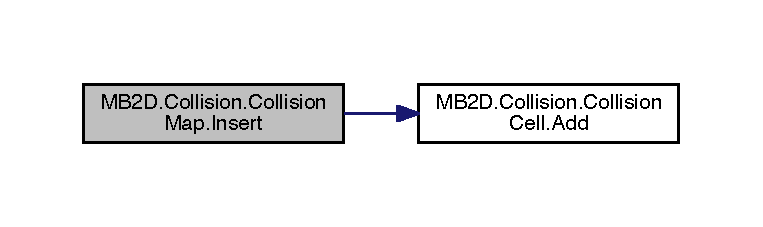
\includegraphics[width=350pt]{class_m_b2_d_1_1_collision_1_1_collision_map_a7d53571c049d50d62e6132413fe712e3_cgraph}
\end{center}
\end{figure}
Here is the caller graph for this function\+:
\nopagebreak
\begin{figure}[H]
\begin{center}
\leavevmode
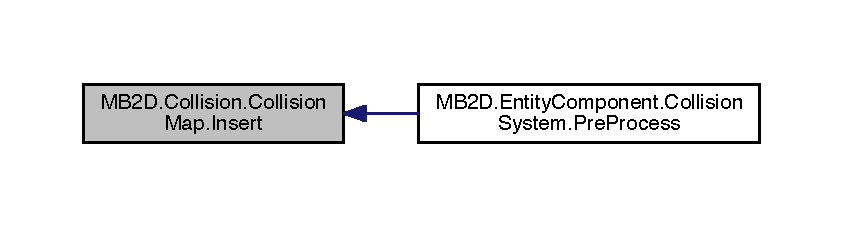
\includegraphics[width=350pt]{class_m_b2_d_1_1_collision_1_1_collision_map_a7d53571c049d50d62e6132413fe712e3_icgraph}
\end{center}
\end{figure}
\hypertarget{class_m_b2_d_1_1_collision_1_1_collision_map_a8f34c934947ce25d7de681fc07f14e09}{}\label{class_m_b2_d_1_1_collision_1_1_collision_map_a8f34c934947ce25d7de681fc07f14e09} 
\index{M\+B2\+D\+::\+Collision\+::\+Collision\+Map@{M\+B2\+D\+::\+Collision\+::\+Collision\+Map}!Update\+Position@{Update\+Position}}
\index{Update\+Position@{Update\+Position}!M\+B2\+D\+::\+Collision\+::\+Collision\+Map@{M\+B2\+D\+::\+Collision\+::\+Collision\+Map}}
\paragraph{\texorpdfstring{Update\+Position()}{UpdatePosition()}}
{\footnotesize\ttfamily void M\+B2\+D.\+Collision.\+Collision\+Map.\+Update\+Position (\begin{DoxyParamCaption}\item[{int}]{x,  }\item[{int}]{y }\end{DoxyParamCaption})\hspace{0.3cm}{\ttfamily [inline]}}



Updates the position of the collision grid. 


\begin{DoxyParams}{Parameters}
{\em x} & The x coordinate.\\
\hline
{\em y} & The y coordinate.\\
\hline
\end{DoxyParams}


\subsubsection{Property Documentation}
\hypertarget{class_m_b2_d_1_1_collision_1_1_collision_map_aacfa35801f16fad4ea0d128edf522095}{}\label{class_m_b2_d_1_1_collision_1_1_collision_map_aacfa35801f16fad4ea0d128edf522095} 
\index{M\+B2\+D\+::\+Collision\+::\+Collision\+Map@{M\+B2\+D\+::\+Collision\+::\+Collision\+Map}!Grid@{Grid}}
\index{Grid@{Grid}!M\+B2\+D\+::\+Collision\+::\+Collision\+Map@{M\+B2\+D\+::\+Collision\+::\+Collision\+Map}}
\paragraph{\texorpdfstring{Grid}{Grid}}
{\footnotesize\ttfamily \hyperlink{class_m_b2_d_1_1_geometry_1_1_grid}{Grid} M\+B2\+D.\+Collision.\+Collision\+Map.\+Grid\hspace{0.3cm}{\ttfamily [get]}}



Gets the geometric representation of the grid 

The grid.\hypertarget{class_m_b2_d_1_1_collision_1_1_collision_map_a707dab6ca65cfe316c248976a0d750f6}{}\label{class_m_b2_d_1_1_collision_1_1_collision_map_a707dab6ca65cfe316c248976a0d750f6} 
\index{M\+B2\+D\+::\+Collision\+::\+Collision\+Map@{M\+B2\+D\+::\+Collision\+::\+Collision\+Map}!Max@{Max}}
\index{Max@{Max}!M\+B2\+D\+::\+Collision\+::\+Collision\+Map@{M\+B2\+D\+::\+Collision\+::\+Collision\+Map}}
\paragraph{\texorpdfstring{Max}{Max}}
{\footnotesize\ttfamily Vector2 M\+B2\+D.\+Collision.\+Collision\+Map.\+Max\hspace{0.3cm}{\ttfamily [get]}}



Gets the upper bounds of the x and y coordinates in the grid 

The max coordinates.\hypertarget{class_m_b2_d_1_1_collision_1_1_collision_map_a0d069be50f64db9f09d488dc2642ee48}{}\label{class_m_b2_d_1_1_collision_1_1_collision_map_a0d069be50f64db9f09d488dc2642ee48} 
\index{M\+B2\+D\+::\+Collision\+::\+Collision\+Map@{M\+B2\+D\+::\+Collision\+::\+Collision\+Map}!Position@{Position}}
\index{Position@{Position}!M\+B2\+D\+::\+Collision\+::\+Collision\+Map@{M\+B2\+D\+::\+Collision\+::\+Collision\+Map}}
\paragraph{\texorpdfstring{Position}{Position}}
{\footnotesize\ttfamily Vector2 M\+B2\+D.\+Collision.\+Collision\+Map.\+Position\hspace{0.3cm}{\ttfamily [get]}}



Gets the current position of the grid. 

The position.

The documentation for this class was generated from the following file\+:\begin{DoxyCompactItemize}
\item 
M\+B2\+D/src/\+Collision/Collision\+Map.\+cs\end{DoxyCompactItemize}

\hypertarget{class_m_b2_d_1_1_testing_1_1_collision_render_system}{}\section{M\+B2\+D.\+Testing.\+Collision\+Render\+System Class Reference}
\label{class_m_b2_d_1_1_testing_1_1_collision_render_system}\index{M\+B2\+D.\+Testing.\+Collision\+Render\+System@{M\+B2\+D.\+Testing.\+Collision\+Render\+System}}


Inheritance diagram for M\+B2\+D.\+Testing.\+Collision\+Render\+System\+:\nopagebreak
\begin{figure}[H]
\begin{center}
\leavevmode
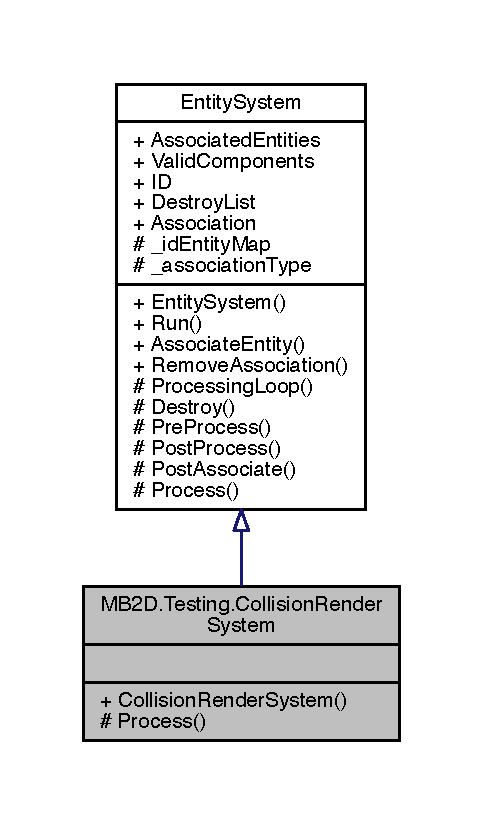
\includegraphics[width=232pt]{class_m_b2_d_1_1_testing_1_1_collision_render_system__inherit__graph}
\end{center}
\end{figure}


Collaboration diagram for M\+B2\+D.\+Testing.\+Collision\+Render\+System\+:\nopagebreak
\begin{figure}[H]
\begin{center}
\leavevmode
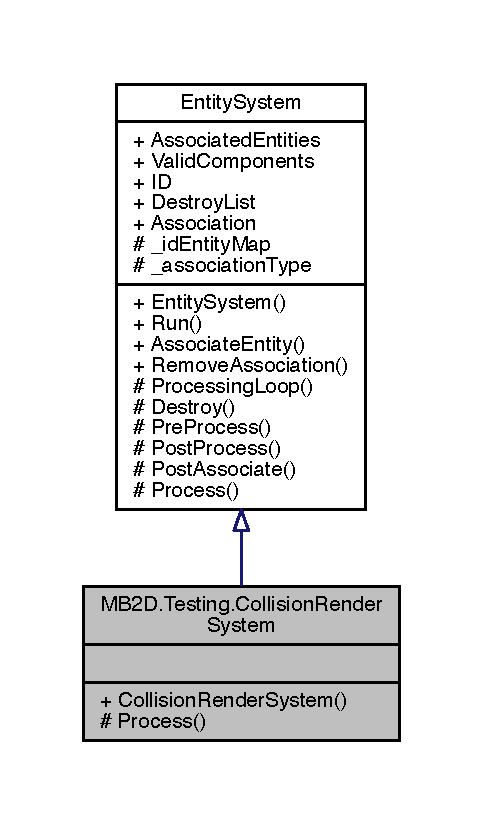
\includegraphics[width=232pt]{class_m_b2_d_1_1_testing_1_1_collision_render_system__coll__graph}
\end{center}
\end{figure}
\subsection*{Public Member Functions}
\begin{DoxyCompactItemize}
\item 
\hypertarget{class_m_b2_d_1_1_testing_1_1_collision_render_system_a6fc7755e518e6138a5b02f5af7d7e460}{}\label{class_m_b2_d_1_1_testing_1_1_collision_render_system_a6fc7755e518e6138a5b02f5af7d7e460} 
{\bfseries Collision\+Render\+System} (Sprite\+Batch sprite\+Batch)
\end{DoxyCompactItemize}
\subsection*{Protected Member Functions}
\begin{DoxyCompactItemize}
\item 
override void \hyperlink{class_m_b2_d_1_1_testing_1_1_collision_render_system_af7b7ffdb316533a084e98cbea97a096f}{Process} (\hyperlink{class_m_b2_d_1_1_entity_component_1_1_entity}{Entity} entity)
\begin{DoxyCompactList}\small\item\em Executes this systems logic on a single entity \end{DoxyCompactList}\end{DoxyCompactItemize}
\subsection*{Additional Inherited Members}


\subsection{Member Function Documentation}
\hypertarget{class_m_b2_d_1_1_testing_1_1_collision_render_system_af7b7ffdb316533a084e98cbea97a096f}{}\label{class_m_b2_d_1_1_testing_1_1_collision_render_system_af7b7ffdb316533a084e98cbea97a096f} 
\index{M\+B2\+D\+::\+Testing\+::\+Collision\+Render\+System@{M\+B2\+D\+::\+Testing\+::\+Collision\+Render\+System}!Process@{Process}}
\index{Process@{Process}!M\+B2\+D\+::\+Testing\+::\+Collision\+Render\+System@{M\+B2\+D\+::\+Testing\+::\+Collision\+Render\+System}}
\subsubsection{\texorpdfstring{Process()}{Process()}}
{\footnotesize\ttfamily override void M\+B2\+D.\+Testing.\+Collision\+Render\+System.\+Process (\begin{DoxyParamCaption}\item[{\hyperlink{class_m_b2_d_1_1_entity_component_1_1_entity}{Entity}}]{entity }\end{DoxyParamCaption})\hspace{0.3cm}{\ttfamily [inline]}, {\ttfamily [protected]}, {\ttfamily [virtual]}}



Executes this systems logic on a single entity 


\begin{DoxyParams}{Parameters}
{\em entity} & Entity to operate on\\
\hline
\end{DoxyParams}


Implements \hyperlink{class_m_b2_d_1_1_entity_component_1_1_entity_system_abbf83b87cb5d12754fb058cef50451fa}{M\+B2\+D.\+Entity\+Component.\+Entity\+System}.



The documentation for this class was generated from the following file\+:\begin{DoxyCompactItemize}
\item 
M\+B2\+D/src/\+Test/Collision\+Render\+System.\+cs\end{DoxyCompactItemize}

\hypertarget{class_m_b2_d_1_1_entity_component_1_1_collision_system}{}\section{M\+B2\+D.\+Entity\+Component.\+Collision\+System Class Reference}
\label{class_m_b2_d_1_1_entity_component_1_1_collision_system}\index{M\+B2\+D.\+Entity\+Component.\+Collision\+System@{M\+B2\+D.\+Entity\+Component.\+Collision\+System}}


Checks collisions. Uses a spatial indexing grid for broad-\/phase collision checking and A\+A\+BB checks for narrow phase  




Inheritance diagram for M\+B2\+D.\+Entity\+Component.\+Collision\+System\+:
\nopagebreak
\begin{figure}[H]
\begin{center}
\leavevmode
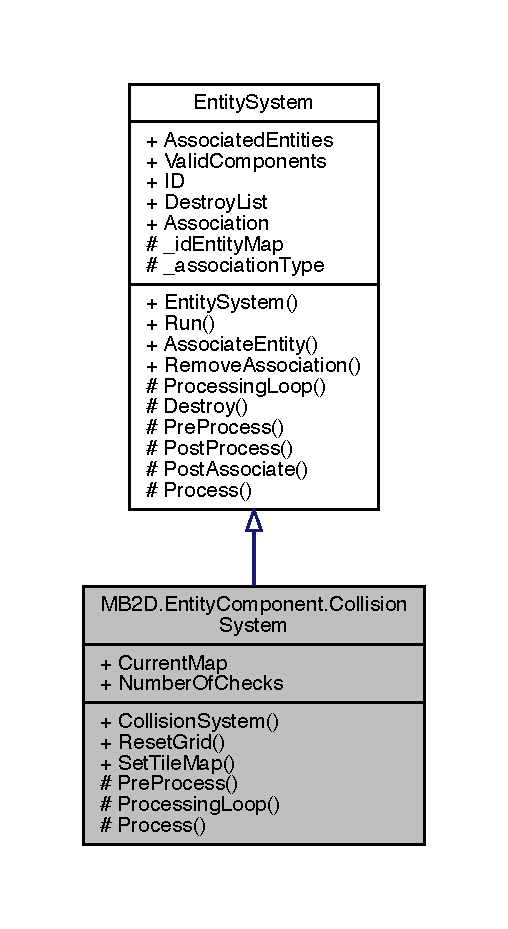
\includegraphics[width=244pt]{class_m_b2_d_1_1_entity_component_1_1_collision_system__inherit__graph}
\end{center}
\end{figure}


Collaboration diagram for M\+B2\+D.\+Entity\+Component.\+Collision\+System\+:
\nopagebreak
\begin{figure}[H]
\begin{center}
\leavevmode
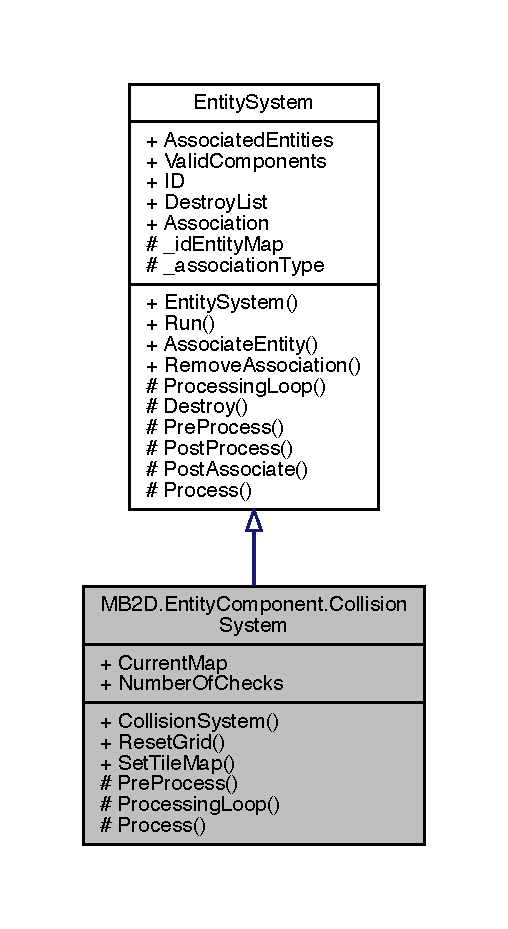
\includegraphics[width=244pt]{class_m_b2_d_1_1_entity_component_1_1_collision_system__coll__graph}
\end{center}
\end{figure}
\subsection*{Public Member Functions}
\begin{DoxyCompactItemize}
\item 
\hyperlink{class_m_b2_d_1_1_entity_component_1_1_collision_system_ac6452aea90e8ee3376b8ea0e089bebc1}{Collision\+System} ()
\begin{DoxyCompactList}\small\item\em Initializes a new instance of the T\+:\+M\+B2\+D.\+Entity\+Component.\+Collision\+System class. \end{DoxyCompactList}\item 
void \hyperlink{class_m_b2_d_1_1_entity_component_1_1_collision_system_a682979b3b811fede89b625cc42b6342c}{Reset\+Grid} (int x\+Min, int x\+Max, int y\+Min, int y\+Max, int cell\+Size)
\begin{DoxyCompactList}\small\item\em Resets the grid position in the world. \end{DoxyCompactList}\item 
void \hyperlink{class_m_b2_d_1_1_entity_component_1_1_collision_system_a4710a6cf7aba7b5ba9c75e0771793b93}{Set\+Tile\+Map} (\hyperlink{class_m_b2_d_1_1_tiles_1_1_tile_map}{Tile\+Map} tile\+Map)
\begin{DoxyCompactList}\small\item\em Sets the current tile map to check for collisions \end{DoxyCompactList}\end{DoxyCompactItemize}
\subsection*{Protected Member Functions}
\begin{DoxyCompactItemize}
\item 
override void \hyperlink{class_m_b2_d_1_1_entity_component_1_1_collision_system_ad591227767c8b6c66ca3891de04e9050}{Pre\+Process} ()
\begin{DoxyCompactList}\small\item\em Clears the collision grid and inserts all entities before checking collisions \end{DoxyCompactList}\item 
override void \hyperlink{class_m_b2_d_1_1_entity_component_1_1_collision_system_a06249adc606475cdc35f28783a1b27c4}{Processing\+Loop} ()
\begin{DoxyCompactList}\small\item\em Override. Only processes entities with movement components. Still considers static entities, but only as possible neighbours. \end{DoxyCompactList}\item 
override void \hyperlink{class_m_b2_d_1_1_entity_component_1_1_collision_system_adfbee070ed7b120565a5f8a08c159535}{Process} (\hyperlink{class_m_b2_d_1_1_entity_component_1_1_entity}{Entity} entity)
\begin{DoxyCompactList}\small\item\em Checks all collisions within the entities known collision cells \end{DoxyCompactList}\end{DoxyCompactItemize}
\subsection*{Properties}
\begin{DoxyCompactItemize}
\item 
\hyperlink{class_m_b2_d_1_1_collision_1_1_collision_map}{Collision\+Map} \hyperlink{class_m_b2_d_1_1_entity_component_1_1_collision_system_a338aebc3f288cf68926074026af3dbba}{Current\+Map}\hspace{0.3cm}{\ttfamily  \mbox{[}get\mbox{]}}
\begin{DoxyCompactList}\small\item\em Gets the current collision map. \end{DoxyCompactList}\item 
int \hyperlink{class_m_b2_d_1_1_entity_component_1_1_collision_system_a9448df47918780c8287b6f7ff177d46f}{Number\+Of\+Checks}\hspace{0.3cm}{\ttfamily  \mbox{[}get\mbox{]}}
\begin{DoxyCompactList}\small\item\em Gets the number of collision checks made last frame. Used for debugging. \end{DoxyCompactList}\end{DoxyCompactItemize}
\subsection*{Additional Inherited Members}


\subsection{Detailed Description}
Checks collisions. Uses a spatial indexing grid for broad-\/phase collision checking and A\+A\+BB checks for narrow phase 



\subsection{Constructor \& Destructor Documentation}
\hypertarget{class_m_b2_d_1_1_entity_component_1_1_collision_system_ac6452aea90e8ee3376b8ea0e089bebc1}{}\label{class_m_b2_d_1_1_entity_component_1_1_collision_system_ac6452aea90e8ee3376b8ea0e089bebc1} 
\index{M\+B2\+D\+::\+Entity\+Component\+::\+Collision\+System@{M\+B2\+D\+::\+Entity\+Component\+::\+Collision\+System}!Collision\+System@{Collision\+System}}
\index{Collision\+System@{Collision\+System}!M\+B2\+D\+::\+Entity\+Component\+::\+Collision\+System@{M\+B2\+D\+::\+Entity\+Component\+::\+Collision\+System}}
\subsubsection{\texorpdfstring{Collision\+System()}{CollisionSystem()}}
{\footnotesize\ttfamily M\+B2\+D.\+Entity\+Component.\+Collision\+System.\+Collision\+System (\begin{DoxyParamCaption}{ }\end{DoxyParamCaption})\hspace{0.3cm}{\ttfamily [inline]}}



Initializes a new instance of the T\+:\+M\+B2\+D.\+Entity\+Component.\+Collision\+System class. 



\subsection{Member Function Documentation}
\hypertarget{class_m_b2_d_1_1_entity_component_1_1_collision_system_ad591227767c8b6c66ca3891de04e9050}{}\label{class_m_b2_d_1_1_entity_component_1_1_collision_system_ad591227767c8b6c66ca3891de04e9050} 
\index{M\+B2\+D\+::\+Entity\+Component\+::\+Collision\+System@{M\+B2\+D\+::\+Entity\+Component\+::\+Collision\+System}!Pre\+Process@{Pre\+Process}}
\index{Pre\+Process@{Pre\+Process}!M\+B2\+D\+::\+Entity\+Component\+::\+Collision\+System@{M\+B2\+D\+::\+Entity\+Component\+::\+Collision\+System}}
\subsubsection{\texorpdfstring{Pre\+Process()}{PreProcess()}}
{\footnotesize\ttfamily override void M\+B2\+D.\+Entity\+Component.\+Collision\+System.\+Pre\+Process (\begin{DoxyParamCaption}{ }\end{DoxyParamCaption})\hspace{0.3cm}{\ttfamily [inline]}, {\ttfamily [protected]}, {\ttfamily [virtual]}}



Clears the collision grid and inserts all entities before checking collisions 



Reimplemented from \hyperlink{class_m_b2_d_1_1_entity_component_1_1_entity_system_aadc002dd04d9cb75775ca955a28e303e}{M\+B2\+D.\+Entity\+Component.\+Entity\+System}.

Here is the call graph for this function\+:
\nopagebreak
\begin{figure}[H]
\begin{center}
\leavevmode
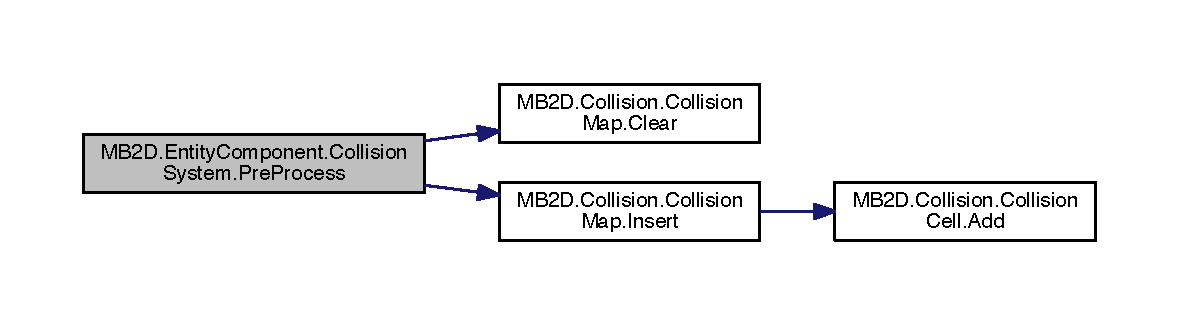
\includegraphics[width=350pt]{class_m_b2_d_1_1_entity_component_1_1_collision_system_ad591227767c8b6c66ca3891de04e9050_cgraph}
\end{center}
\end{figure}
\hypertarget{class_m_b2_d_1_1_entity_component_1_1_collision_system_adfbee070ed7b120565a5f8a08c159535}{}\label{class_m_b2_d_1_1_entity_component_1_1_collision_system_adfbee070ed7b120565a5f8a08c159535} 
\index{M\+B2\+D\+::\+Entity\+Component\+::\+Collision\+System@{M\+B2\+D\+::\+Entity\+Component\+::\+Collision\+System}!Process@{Process}}
\index{Process@{Process}!M\+B2\+D\+::\+Entity\+Component\+::\+Collision\+System@{M\+B2\+D\+::\+Entity\+Component\+::\+Collision\+System}}
\subsubsection{\texorpdfstring{Process()}{Process()}}
{\footnotesize\ttfamily override void M\+B2\+D.\+Entity\+Component.\+Collision\+System.\+Process (\begin{DoxyParamCaption}\item[{\hyperlink{class_m_b2_d_1_1_entity_component_1_1_entity}{Entity}}]{entity }\end{DoxyParamCaption})\hspace{0.3cm}{\ttfamily [inline]}, {\ttfamily [protected]}, {\ttfamily [virtual]}}



Checks all collisions within the entities known collision cells 


\begin{DoxyParams}{Parameters}
{\em entity} & \hyperlink{class_m_b2_d_1_1_entity_component_1_1_entity}{Entity} to check.\\
\hline
\end{DoxyParams}


Implements \hyperlink{class_m_b2_d_1_1_entity_component_1_1_entity_system_abbf83b87cb5d12754fb058cef50451fa}{M\+B2\+D.\+Entity\+Component.\+Entity\+System}.

Here is the call graph for this function\+:
\nopagebreak
\begin{figure}[H]
\begin{center}
\leavevmode
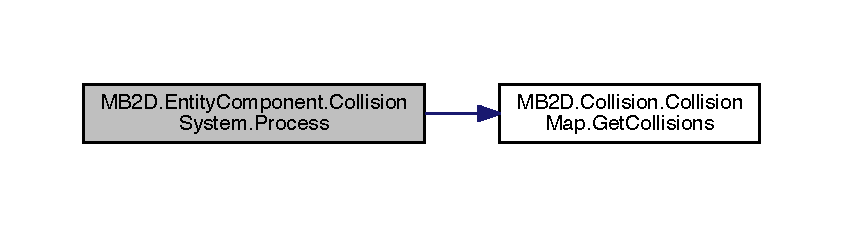
\includegraphics[width=350pt]{class_m_b2_d_1_1_entity_component_1_1_collision_system_adfbee070ed7b120565a5f8a08c159535_cgraph}
\end{center}
\end{figure}
\hypertarget{class_m_b2_d_1_1_entity_component_1_1_collision_system_a06249adc606475cdc35f28783a1b27c4}{}\label{class_m_b2_d_1_1_entity_component_1_1_collision_system_a06249adc606475cdc35f28783a1b27c4} 
\index{M\+B2\+D\+::\+Entity\+Component\+::\+Collision\+System@{M\+B2\+D\+::\+Entity\+Component\+::\+Collision\+System}!Processing\+Loop@{Processing\+Loop}}
\index{Processing\+Loop@{Processing\+Loop}!M\+B2\+D\+::\+Entity\+Component\+::\+Collision\+System@{M\+B2\+D\+::\+Entity\+Component\+::\+Collision\+System}}
\subsubsection{\texorpdfstring{Processing\+Loop()}{ProcessingLoop()}}
{\footnotesize\ttfamily override void M\+B2\+D.\+Entity\+Component.\+Collision\+System.\+Processing\+Loop (\begin{DoxyParamCaption}{ }\end{DoxyParamCaption})\hspace{0.3cm}{\ttfamily [inline]}, {\ttfamily [protected]}, {\ttfamily [virtual]}}



Override. Only processes entities with movement components. Still considers static entities, but only as possible neighbours. 



Reimplemented from \hyperlink{class_m_b2_d_1_1_entity_component_1_1_entity_system_a75552787342e68c427bf2e1ffa60ed6c}{M\+B2\+D.\+Entity\+Component.\+Entity\+System}.

\hypertarget{class_m_b2_d_1_1_entity_component_1_1_collision_system_a682979b3b811fede89b625cc42b6342c}{}\label{class_m_b2_d_1_1_entity_component_1_1_collision_system_a682979b3b811fede89b625cc42b6342c} 
\index{M\+B2\+D\+::\+Entity\+Component\+::\+Collision\+System@{M\+B2\+D\+::\+Entity\+Component\+::\+Collision\+System}!Reset\+Grid@{Reset\+Grid}}
\index{Reset\+Grid@{Reset\+Grid}!M\+B2\+D\+::\+Entity\+Component\+::\+Collision\+System@{M\+B2\+D\+::\+Entity\+Component\+::\+Collision\+System}}
\subsubsection{\texorpdfstring{Reset\+Grid()}{ResetGrid()}}
{\footnotesize\ttfamily void M\+B2\+D.\+Entity\+Component.\+Collision\+System.\+Reset\+Grid (\begin{DoxyParamCaption}\item[{int}]{x\+Min,  }\item[{int}]{x\+Max,  }\item[{int}]{y\+Min,  }\item[{int}]{y\+Max,  }\item[{int}]{cell\+Size }\end{DoxyParamCaption})\hspace{0.3cm}{\ttfamily [inline]}}



Resets the grid position in the world. 


\begin{DoxyParams}{Parameters}
{\em x\+Min} & The grids left most x coordinate.\\
\hline
{\em x\+Max} & Right most x coordinae.\\
\hline
{\em y\+Min} & Top most y coordinate.\\
\hline
{\em y\+Max} & Bottom most y coordinate.\\
\hline
{\em cell\+Size} & The size of each cell in the grid.\\
\hline
\end{DoxyParams}
Here is the caller graph for this function\+:
\nopagebreak
\begin{figure}[H]
\begin{center}
\leavevmode
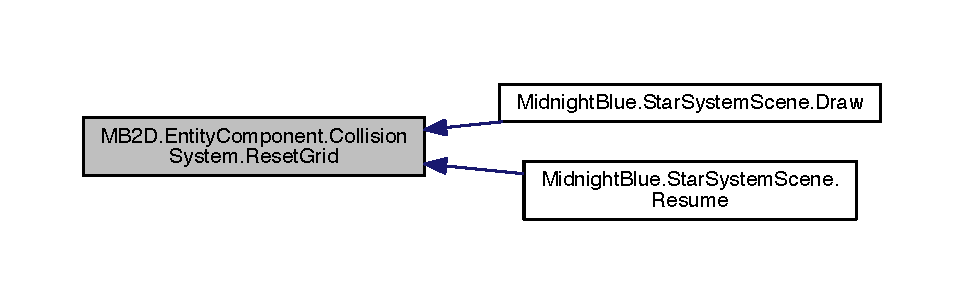
\includegraphics[width=350pt]{class_m_b2_d_1_1_entity_component_1_1_collision_system_a682979b3b811fede89b625cc42b6342c_icgraph}
\end{center}
\end{figure}
\hypertarget{class_m_b2_d_1_1_entity_component_1_1_collision_system_a4710a6cf7aba7b5ba9c75e0771793b93}{}\label{class_m_b2_d_1_1_entity_component_1_1_collision_system_a4710a6cf7aba7b5ba9c75e0771793b93} 
\index{M\+B2\+D\+::\+Entity\+Component\+::\+Collision\+System@{M\+B2\+D\+::\+Entity\+Component\+::\+Collision\+System}!Set\+Tile\+Map@{Set\+Tile\+Map}}
\index{Set\+Tile\+Map@{Set\+Tile\+Map}!M\+B2\+D\+::\+Entity\+Component\+::\+Collision\+System@{M\+B2\+D\+::\+Entity\+Component\+::\+Collision\+System}}
\subsubsection{\texorpdfstring{Set\+Tile\+Map()}{SetTileMap()}}
{\footnotesize\ttfamily void M\+B2\+D.\+Entity\+Component.\+Collision\+System.\+Set\+Tile\+Map (\begin{DoxyParamCaption}\item[{\hyperlink{class_m_b2_d_1_1_tiles_1_1_tile_map}{Tile\+Map}}]{tile\+Map }\end{DoxyParamCaption})\hspace{0.3cm}{\ttfamily [inline]}}



Sets the current tile map to check for collisions 


\begin{DoxyParams}{Parameters}
{\em tile\+Map} & \hyperlink{class_m_b2_d_1_1_tile}{Tile} map.\\
\hline
\end{DoxyParams}
Here is the caller graph for this function\+:
\nopagebreak
\begin{figure}[H]
\begin{center}
\leavevmode
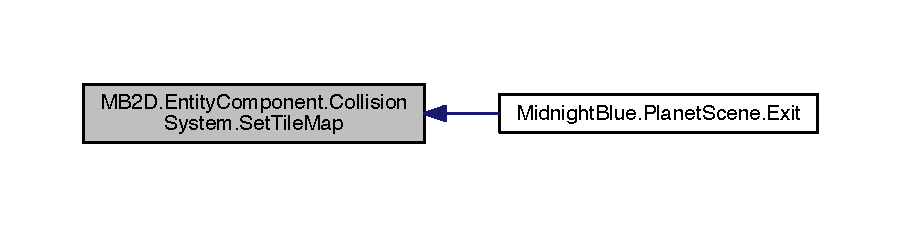
\includegraphics[width=350pt]{class_m_b2_d_1_1_entity_component_1_1_collision_system_a4710a6cf7aba7b5ba9c75e0771793b93_icgraph}
\end{center}
\end{figure}


\subsection{Property Documentation}
\hypertarget{class_m_b2_d_1_1_entity_component_1_1_collision_system_a338aebc3f288cf68926074026af3dbba}{}\label{class_m_b2_d_1_1_entity_component_1_1_collision_system_a338aebc3f288cf68926074026af3dbba} 
\index{M\+B2\+D\+::\+Entity\+Component\+::\+Collision\+System@{M\+B2\+D\+::\+Entity\+Component\+::\+Collision\+System}!Current\+Map@{Current\+Map}}
\index{Current\+Map@{Current\+Map}!M\+B2\+D\+::\+Entity\+Component\+::\+Collision\+System@{M\+B2\+D\+::\+Entity\+Component\+::\+Collision\+System}}
\subsubsection{\texorpdfstring{Current\+Map}{CurrentMap}}
{\footnotesize\ttfamily \hyperlink{class_m_b2_d_1_1_collision_1_1_collision_map}{Collision\+Map} M\+B2\+D.\+Entity\+Component.\+Collision\+System.\+Current\+Map\hspace{0.3cm}{\ttfamily [get]}}



Gets the current collision map. 

The current map.\hypertarget{class_m_b2_d_1_1_entity_component_1_1_collision_system_a9448df47918780c8287b6f7ff177d46f}{}\label{class_m_b2_d_1_1_entity_component_1_1_collision_system_a9448df47918780c8287b6f7ff177d46f} 
\index{M\+B2\+D\+::\+Entity\+Component\+::\+Collision\+System@{M\+B2\+D\+::\+Entity\+Component\+::\+Collision\+System}!Number\+Of\+Checks@{Number\+Of\+Checks}}
\index{Number\+Of\+Checks@{Number\+Of\+Checks}!M\+B2\+D\+::\+Entity\+Component\+::\+Collision\+System@{M\+B2\+D\+::\+Entity\+Component\+::\+Collision\+System}}
\subsubsection{\texorpdfstring{Number\+Of\+Checks}{NumberOfChecks}}
{\footnotesize\ttfamily int M\+B2\+D.\+Entity\+Component.\+Collision\+System.\+Number\+Of\+Checks\hspace{0.3cm}{\ttfamily [get]}}



Gets the number of collision checks made last frame. Used for debugging. 

The number of collision checks.

The documentation for this class was generated from the following file\+:\begin{DoxyCompactItemize}
\item 
M\+B2\+D/src/\+Entity\+Component/\+Systems/Collision\+System.\+cs\end{DoxyCompactItemize}

\hypertarget{class_m_b2_d_1_1_i_o_1_1_command}{}\subsection{M\+B2\+D.\+I\+O.\+Command Class Reference}
\label{class_m_b2_d_1_1_i_o_1_1_command}\index{M\+B2\+D.\+I\+O.\+Command@{M\+B2\+D.\+I\+O.\+Command}}


Executes an action associated with a specific key  




Inheritance diagram for M\+B2\+D.\+I\+O.\+Command\+:
\nopagebreak
\begin{figure}[H]
\begin{center}
\leavevmode
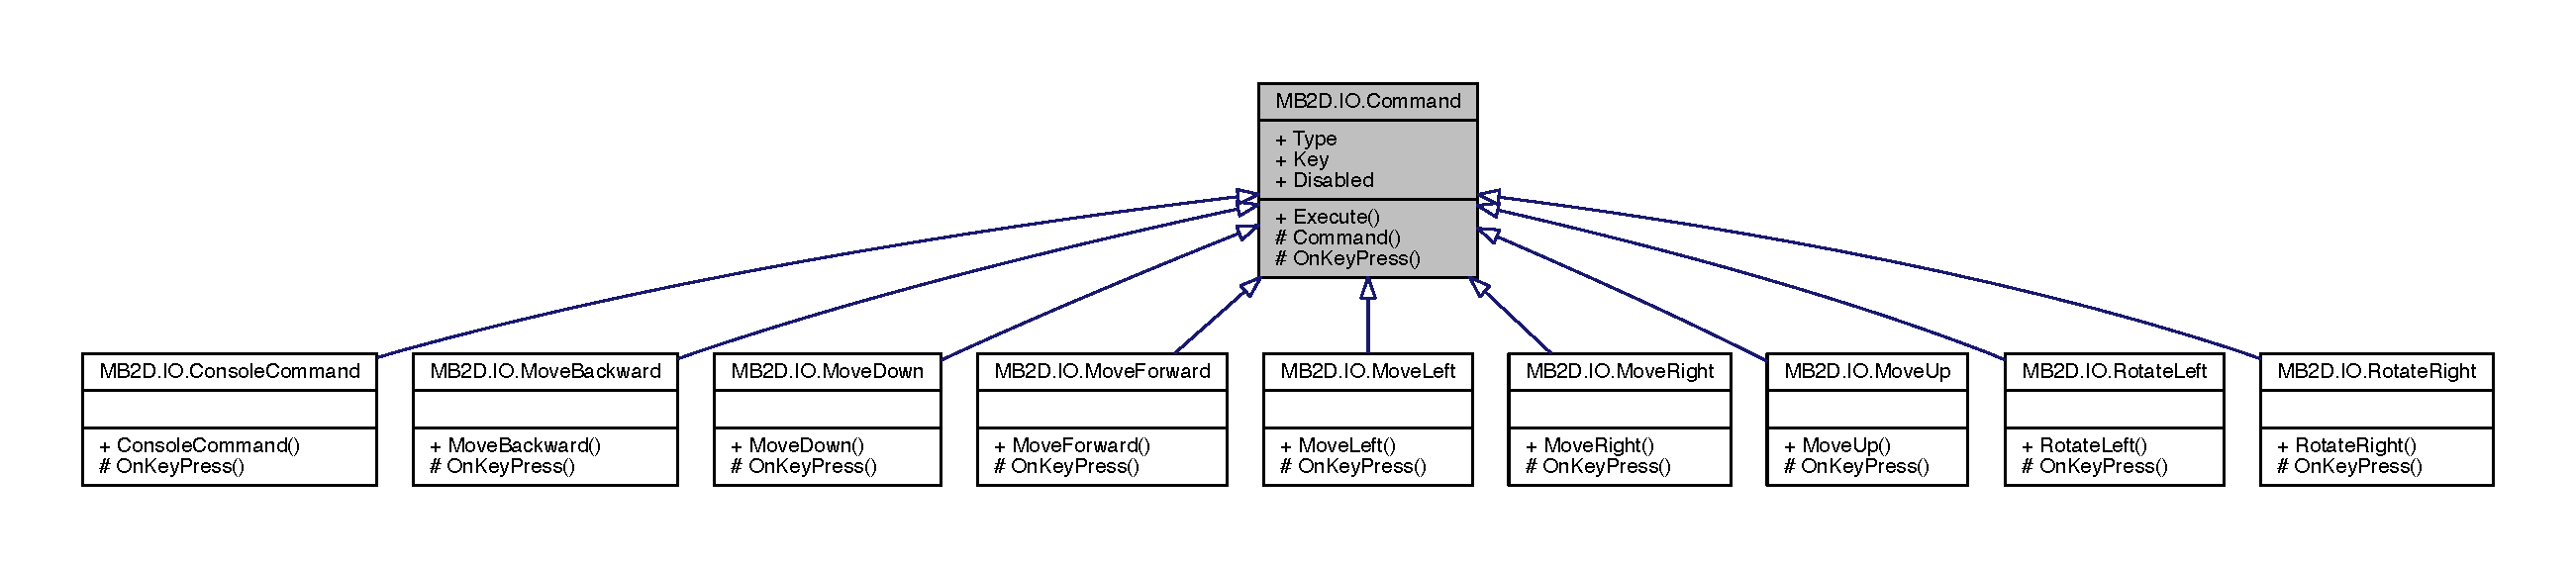
\includegraphics[width=350pt]{class_m_b2_d_1_1_i_o_1_1_command__inherit__graph}
\end{center}
\end{figure}


Collaboration diagram for M\+B2\+D.\+I\+O.\+Command\+:
\nopagebreak
\begin{figure}[H]
\begin{center}
\leavevmode
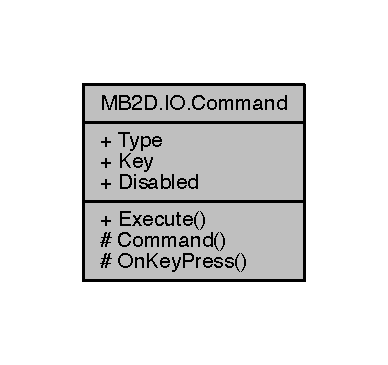
\includegraphics[width=186pt]{class_m_b2_d_1_1_i_o_1_1_command__coll__graph}
\end{center}
\end{figure}
\subsubsection*{Public Member Functions}
\begin{DoxyCompactItemize}
\item 
bool \hyperlink{class_m_b2_d_1_1_i_o_1_1_command_a59f97dd5810dd5b112c82ad3758da7e8}{Execute} (\hyperlink{class_m_b2_d_1_1_entity_component_1_1_entity}{Entity} e=null)
\begin{DoxyCompactList}\small\item\em Executes the specific command on the entity parameter \end{DoxyCompactList}\end{DoxyCompactItemize}
\subsubsection*{Protected Member Functions}
\begin{DoxyCompactItemize}
\item 
\hyperlink{class_m_b2_d_1_1_i_o_1_1_command_a9cb2200e1b56437406cb300a782a425f}{Command} (Keys key, \hyperlink{namespace_m_b2_d_1_1_i_o_ab5f95f3fe9e652778b62bdf943168a68}{Command\+Type} command\+Type)
\begin{DoxyCompactList}\small\item\em Initializes a new instance of the T\+:\+Midnight\+Blue.\+Command class. \end{DoxyCompactList}\item 
abstract void \hyperlink{class_m_b2_d_1_1_i_o_1_1_command_ae927e36c0e285848325cc68eddb5fd72}{On\+Key\+Press} (\hyperlink{class_m_b2_d_1_1_entity_component_1_1_entity}{Entity} e=null)
\begin{DoxyCompactList}\small\item\em Defines the logic to perform when operating on a given entity \end{DoxyCompactList}\end{DoxyCompactItemize}
\subsubsection*{Properties}
\begin{DoxyCompactItemize}
\item 
\hyperlink{namespace_m_b2_d_1_1_i_o_ab5f95f3fe9e652778b62bdf943168a68}{Command\+Type} \hyperlink{class_m_b2_d_1_1_i_o_1_1_command_afd1e0b56bee6e683db89a55c3b155f9b}{Type}\hspace{0.3cm}{\ttfamily  \mbox{[}get, set\mbox{]}}
\begin{DoxyCompactList}\small\item\em Gets or sets the trigger type of the command. \end{DoxyCompactList}\item 
Keys \hyperlink{class_m_b2_d_1_1_i_o_1_1_command_a42f1ab4c0c10b351e296d23713bd0a6a}{Key}\hspace{0.3cm}{\ttfamily  \mbox{[}get\mbox{]}}
\begin{DoxyCompactList}\small\item\em Gets the keycode associated with the command. \end{DoxyCompactList}\item 
\hypertarget{class_m_b2_d_1_1_i_o_1_1_command_ade6e24126e6d0d094872513b584de862}{}\label{class_m_b2_d_1_1_i_o_1_1_command_ade6e24126e6d0d094872513b584de862} 
bool {\bfseries Disabled}\hspace{0.3cm}{\ttfamily  \mbox{[}get, set\mbox{]}}
\end{DoxyCompactItemize}


\subsubsection{Detailed Description}
Executes an action associated with a specific key 



\subsubsection{Constructor \& Destructor Documentation}
\hypertarget{class_m_b2_d_1_1_i_o_1_1_command_a9cb2200e1b56437406cb300a782a425f}{}\label{class_m_b2_d_1_1_i_o_1_1_command_a9cb2200e1b56437406cb300a782a425f} 
\index{M\+B2\+D\+::\+I\+O\+::\+Command@{M\+B2\+D\+::\+I\+O\+::\+Command}!Command@{Command}}
\index{Command@{Command}!M\+B2\+D\+::\+I\+O\+::\+Command@{M\+B2\+D\+::\+I\+O\+::\+Command}}
\paragraph{\texorpdfstring{Command()}{Command()}}
{\footnotesize\ttfamily M\+B2\+D.\+I\+O.\+Command.\+Command (\begin{DoxyParamCaption}\item[{Keys}]{key,  }\item[{\hyperlink{namespace_m_b2_d_1_1_i_o_ab5f95f3fe9e652778b62bdf943168a68}{Command\+Type}}]{command\+Type }\end{DoxyParamCaption})\hspace{0.3cm}{\ttfamily [inline]}, {\ttfamily [protected]}}



Initializes a new instance of the T\+:\+Midnight\+Blue.\+Command class. 


\begin{DoxyParams}{Parameters}
{\em key} & Key to associate with the command\\
\hline
{\em command\+Type} & Trigger or hold command\\
\hline
\end{DoxyParams}


\subsubsection{Member Function Documentation}
\hypertarget{class_m_b2_d_1_1_i_o_1_1_command_a59f97dd5810dd5b112c82ad3758da7e8}{}\label{class_m_b2_d_1_1_i_o_1_1_command_a59f97dd5810dd5b112c82ad3758da7e8} 
\index{M\+B2\+D\+::\+I\+O\+::\+Command@{M\+B2\+D\+::\+I\+O\+::\+Command}!Execute@{Execute}}
\index{Execute@{Execute}!M\+B2\+D\+::\+I\+O\+::\+Command@{M\+B2\+D\+::\+I\+O\+::\+Command}}
\paragraph{\texorpdfstring{Execute()}{Execute()}}
{\footnotesize\ttfamily bool M\+B2\+D.\+I\+O.\+Command.\+Execute (\begin{DoxyParamCaption}\item[{\hyperlink{class_m_b2_d_1_1_entity_component_1_1_entity}{Entity}}]{e = {\ttfamily null} }\end{DoxyParamCaption})\hspace{0.3cm}{\ttfamily [inline]}}



Executes the specific command on the entity parameter 


\begin{DoxyParams}{Parameters}
{\em e} & Entity to operate on. Optional\\
\hline
\end{DoxyParams}
\hypertarget{class_m_b2_d_1_1_i_o_1_1_command_ae927e36c0e285848325cc68eddb5fd72}{}\label{class_m_b2_d_1_1_i_o_1_1_command_ae927e36c0e285848325cc68eddb5fd72} 
\index{M\+B2\+D\+::\+I\+O\+::\+Command@{M\+B2\+D\+::\+I\+O\+::\+Command}!On\+Key\+Press@{On\+Key\+Press}}
\index{On\+Key\+Press@{On\+Key\+Press}!M\+B2\+D\+::\+I\+O\+::\+Command@{M\+B2\+D\+::\+I\+O\+::\+Command}}
\paragraph{\texorpdfstring{On\+Key\+Press()}{OnKeyPress()}}
{\footnotesize\ttfamily abstract void M\+B2\+D.\+I\+O.\+Command.\+On\+Key\+Press (\begin{DoxyParamCaption}\item[{\hyperlink{class_m_b2_d_1_1_entity_component_1_1_entity}{Entity}}]{e = {\ttfamily null} }\end{DoxyParamCaption})\hspace{0.3cm}{\ttfamily [protected]}, {\ttfamily [pure virtual]}}



Defines the logic to perform when operating on a given entity 


\begin{DoxyParams}{Parameters}
{\em e} & Entity to operate on\\
\hline
\end{DoxyParams}


Implemented in \hyperlink{class_m_b2_d_1_1_i_o_1_1_rotate_left_adf98596b3689a88aaf1334e00b548443}{M\+B2\+D.\+I\+O.\+Rotate\+Left}, \hyperlink{class_m_b2_d_1_1_i_o_1_1_rotate_right_a416106025812db523b009155d462cb6b}{M\+B2\+D.\+I\+O.\+Rotate\+Right}, \hyperlink{class_m_b2_d_1_1_i_o_1_1_move_backward_a15c5da82d35b95c0a04e8fdc89dcd839}{M\+B2\+D.\+I\+O.\+Move\+Backward}, \hyperlink{class_m_b2_d_1_1_i_o_1_1_move_forward_a32d5bfbf101ab8ff8150f2f07f0b5ac8}{M\+B2\+D.\+I\+O.\+Move\+Forward}, \hyperlink{class_m_b2_d_1_1_i_o_1_1_move_left_aa74df62134ee5fc3a5b2503114a5a7e6}{M\+B2\+D.\+I\+O.\+Move\+Left}, \hyperlink{class_m_b2_d_1_1_i_o_1_1_move_down_af93adf7def9f4869528ee2c86b474c19}{M\+B2\+D.\+I\+O.\+Move\+Down}, \hyperlink{class_m_b2_d_1_1_i_o_1_1_move_right_aa0d9913727d27d01dff4fdd394e2f6f4}{M\+B2\+D.\+I\+O.\+Move\+Right}, \hyperlink{class_m_b2_d_1_1_i_o_1_1_move_up_acb3f90aeea44eeffefbb664e898b0a91}{M\+B2\+D.\+I\+O.\+Move\+Up}, and \hyperlink{class_m_b2_d_1_1_i_o_1_1_console_command_ad46e036e534b3b1cd1503782042d358f}{M\+B2\+D.\+I\+O.\+Console\+Command}.



\subsubsection{Property Documentation}
\hypertarget{class_m_b2_d_1_1_i_o_1_1_command_a42f1ab4c0c10b351e296d23713bd0a6a}{}\label{class_m_b2_d_1_1_i_o_1_1_command_a42f1ab4c0c10b351e296d23713bd0a6a} 
\index{M\+B2\+D\+::\+I\+O\+::\+Command@{M\+B2\+D\+::\+I\+O\+::\+Command}!Key@{Key}}
\index{Key@{Key}!M\+B2\+D\+::\+I\+O\+::\+Command@{M\+B2\+D\+::\+I\+O\+::\+Command}}
\paragraph{\texorpdfstring{Key}{Key}}
{\footnotesize\ttfamily Keys M\+B2\+D.\+I\+O.\+Command.\+Key\hspace{0.3cm}{\ttfamily [get]}}



Gets the keycode associated with the command. 

The key code\hypertarget{class_m_b2_d_1_1_i_o_1_1_command_afd1e0b56bee6e683db89a55c3b155f9b}{}\label{class_m_b2_d_1_1_i_o_1_1_command_afd1e0b56bee6e683db89a55c3b155f9b} 
\index{M\+B2\+D\+::\+I\+O\+::\+Command@{M\+B2\+D\+::\+I\+O\+::\+Command}!Type@{Type}}
\index{Type@{Type}!M\+B2\+D\+::\+I\+O\+::\+Command@{M\+B2\+D\+::\+I\+O\+::\+Command}}
\paragraph{\texorpdfstring{Type}{Type}}
{\footnotesize\ttfamily \hyperlink{namespace_m_b2_d_1_1_i_o_ab5f95f3fe9e652778b62bdf943168a68}{Command\+Type} M\+B2\+D.\+I\+O.\+Command.\+Type\hspace{0.3cm}{\ttfamily [get]}, {\ttfamily [set]}}



Gets or sets the trigger type of the command. 

The command type

The documentation for this class was generated from the following file\+:\begin{DoxyCompactItemize}
\item 
M\+B2\+D/src/\+Input/Command.\+cs\end{DoxyCompactItemize}

\hypertarget{class_m_b2_d_1_1_i_o_1_1_console_command}{}\subsection{M\+B2\+D.\+I\+O.\+Console\+Command Class Reference}
\label{class_m_b2_d_1_1_i_o_1_1_console_command}\index{M\+B2\+D.\+I\+O.\+Console\+Command@{M\+B2\+D.\+I\+O.\+Console\+Command}}


Shows or hides the debug console  




Inheritance diagram for M\+B2\+D.\+I\+O.\+Console\+Command\+:
\nopagebreak
\begin{figure}[H]
\begin{center}
\leavevmode
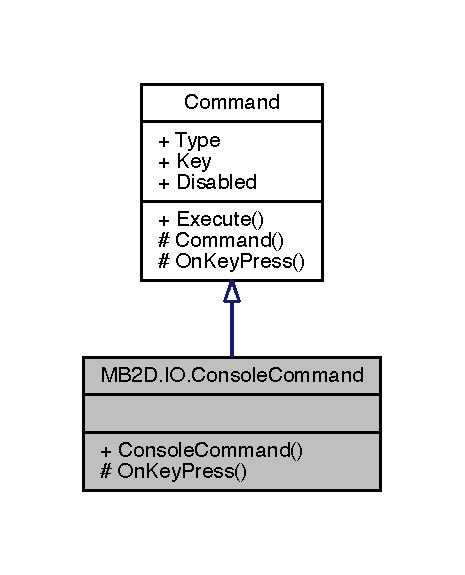
\includegraphics[width=223pt]{class_m_b2_d_1_1_i_o_1_1_console_command__inherit__graph}
\end{center}
\end{figure}


Collaboration diagram for M\+B2\+D.\+I\+O.\+Console\+Command\+:
\nopagebreak
\begin{figure}[H]
\begin{center}
\leavevmode
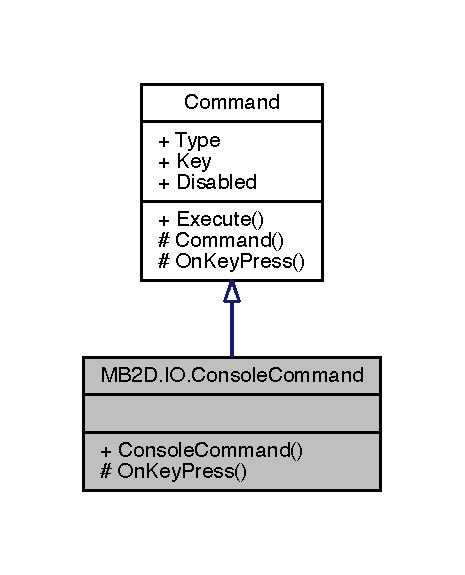
\includegraphics[width=223pt]{class_m_b2_d_1_1_i_o_1_1_console_command__coll__graph}
\end{center}
\end{figure}
\subsubsection*{Public Member Functions}
\begin{DoxyCompactItemize}
\item 
\hyperlink{class_m_b2_d_1_1_i_o_1_1_console_command_a20155e6305233ea1655d9475db692b26}{Console\+Command} (Keys key, \hyperlink{namespace_m_b2_d_1_1_i_o_ab5f95f3fe9e652778b62bdf943168a68}{Command\+Type} type)
\begin{DoxyCompactList}\small\item\em Initializes a new instance of the T\+:\+M\+B2\+D.\+I\+O.\+Console\+Command class. \end{DoxyCompactList}\end{DoxyCompactItemize}
\subsubsection*{Protected Member Functions}
\begin{DoxyCompactItemize}
\item 
override void \hyperlink{class_m_b2_d_1_1_i_o_1_1_console_command_ad46e036e534b3b1cd1503782042d358f}{On\+Key\+Press} (\hyperlink{class_m_b2_d_1_1_entity_component_1_1_entity}{Entity} e=null)
\begin{DoxyCompactList}\small\item\em Toggles the debug console open/closed \end{DoxyCompactList}\end{DoxyCompactItemize}
\subsubsection*{Additional Inherited Members}


\subsubsection{Detailed Description}
Shows or hides the debug console 



\subsubsection{Constructor \& Destructor Documentation}
\hypertarget{class_m_b2_d_1_1_i_o_1_1_console_command_a20155e6305233ea1655d9475db692b26}{}\label{class_m_b2_d_1_1_i_o_1_1_console_command_a20155e6305233ea1655d9475db692b26} 
\index{M\+B2\+D\+::\+I\+O\+::\+Console\+Command@{M\+B2\+D\+::\+I\+O\+::\+Console\+Command}!Console\+Command@{Console\+Command}}
\index{Console\+Command@{Console\+Command}!M\+B2\+D\+::\+I\+O\+::\+Console\+Command@{M\+B2\+D\+::\+I\+O\+::\+Console\+Command}}
\paragraph{\texorpdfstring{Console\+Command()}{ConsoleCommand()}}
{\footnotesize\ttfamily M\+B2\+D.\+I\+O.\+Console\+Command.\+Console\+Command (\begin{DoxyParamCaption}\item[{Keys}]{key,  }\item[{\hyperlink{namespace_m_b2_d_1_1_i_o_ab5f95f3fe9e652778b62bdf943168a68}{Command\+Type}}]{type }\end{DoxyParamCaption})\hspace{0.3cm}{\ttfamily [inline]}}



Initializes a new instance of the T\+:\+M\+B2\+D.\+I\+O.\+Console\+Command class. 


\begin{DoxyParams}{Parameters}
{\em key} & Key to assign the command to.\\
\hline
{\em type} & Type of command trigger.\\
\hline
\end{DoxyParams}


\subsubsection{Member Function Documentation}
\hypertarget{class_m_b2_d_1_1_i_o_1_1_console_command_ad46e036e534b3b1cd1503782042d358f}{}\label{class_m_b2_d_1_1_i_o_1_1_console_command_ad46e036e534b3b1cd1503782042d358f} 
\index{M\+B2\+D\+::\+I\+O\+::\+Console\+Command@{M\+B2\+D\+::\+I\+O\+::\+Console\+Command}!On\+Key\+Press@{On\+Key\+Press}}
\index{On\+Key\+Press@{On\+Key\+Press}!M\+B2\+D\+::\+I\+O\+::\+Console\+Command@{M\+B2\+D\+::\+I\+O\+::\+Console\+Command}}
\paragraph{\texorpdfstring{On\+Key\+Press()}{OnKeyPress()}}
{\footnotesize\ttfamily override void M\+B2\+D.\+I\+O.\+Console\+Command.\+On\+Key\+Press (\begin{DoxyParamCaption}\item[{\hyperlink{class_m_b2_d_1_1_entity_component_1_1_entity}{Entity}}]{e = {\ttfamily null} }\end{DoxyParamCaption})\hspace{0.3cm}{\ttfamily [inline]}, {\ttfamily [protected]}, {\ttfamily [virtual]}}



Toggles the debug console open/closed 


\begin{DoxyParams}{Parameters}
{\em e} & Entity with the controller component. Unused.\\
\hline
\end{DoxyParams}


Implements \hyperlink{class_m_b2_d_1_1_i_o_1_1_command_ae927e36c0e285848325cc68eddb5fd72}{M\+B2\+D.\+I\+O.\+Command}.

Here is the call graph for this function\+:
\nopagebreak
\begin{figure}[H]
\begin{center}
\leavevmode
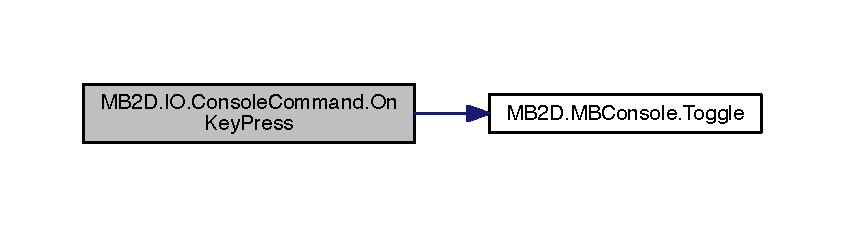
\includegraphics[width=350pt]{class_m_b2_d_1_1_i_o_1_1_console_command_ad46e036e534b3b1cd1503782042d358f_cgraph}
\end{center}
\end{figure}


The documentation for this class was generated from the following file\+:\begin{DoxyCompactItemize}
\item 
M\+B2\+D/src/\+Input/Console\+Command.\+cs\end{DoxyCompactItemize}

\hypertarget{class_m_b2_d_1_1_entity_component_1_1_depth}{}\subsection{M\+B2\+D.\+Entity\+Component.\+Depth Class Reference}
\label{class_m_b2_d_1_1_entity_component_1_1_depth}\index{M\+B2\+D.\+Entity\+Component.\+Depth@{M\+B2\+D.\+Entity\+Component.\+Depth}}


A tag class used to define an entity that should be draw sorted according to its current z-\/index  




Inheritance diagram for M\+B2\+D.\+Entity\+Component.\+Depth\+:
\nopagebreak
\begin{figure}[H]
\begin{center}
\leavevmode
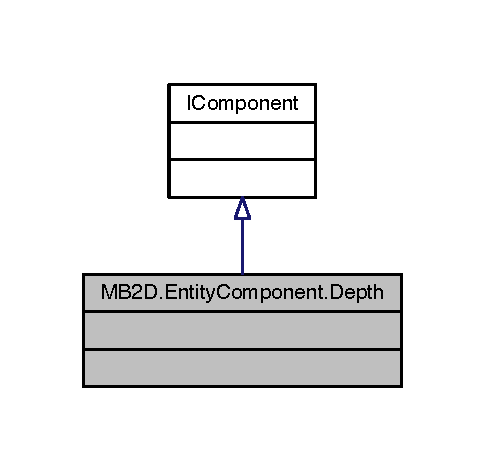
\includegraphics[width=233pt]{class_m_b2_d_1_1_entity_component_1_1_depth__inherit__graph}
\end{center}
\end{figure}


Collaboration diagram for M\+B2\+D.\+Entity\+Component.\+Depth\+:
\nopagebreak
\begin{figure}[H]
\begin{center}
\leavevmode
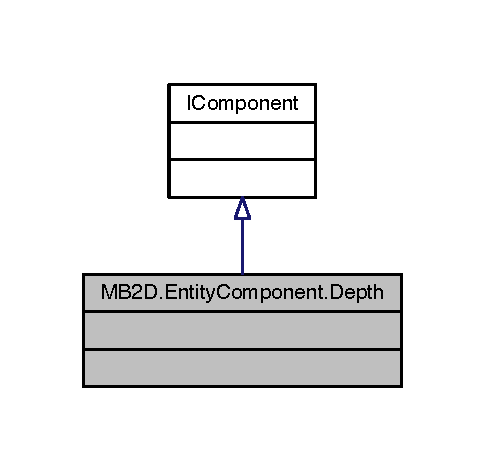
\includegraphics[width=233pt]{class_m_b2_d_1_1_entity_component_1_1_depth__coll__graph}
\end{center}
\end{figure}


\subsubsection{Detailed Description}
A tag class used to define an entity that should be draw sorted according to its current z-\/index 



The documentation for this class was generated from the following file\+:\begin{DoxyCompactItemize}
\item 
M\+B2\+D/src/\+Entity\+Component/\+Components/Depth.\+cs\end{DoxyCompactItemize}

\hypertarget{class_m_b2_d_1_1_entity_component_1_1_depth_system}{}\section{M\+B2\+D.\+Entity\+Component.\+Depth\+System Class Reference}
\label{class_m_b2_d_1_1_entity_component_1_1_depth_system}\index{M\+B2\+D.\+Entity\+Component.\+Depth\+System@{M\+B2\+D.\+Entity\+Component.\+Depth\+System}}


Changes an entities z-\/index based on the y coordinate of the top of their sprite  




Inheritance diagram for M\+B2\+D.\+Entity\+Component.\+Depth\+System\+:
\nopagebreak
\begin{figure}[H]
\begin{center}
\leavevmode
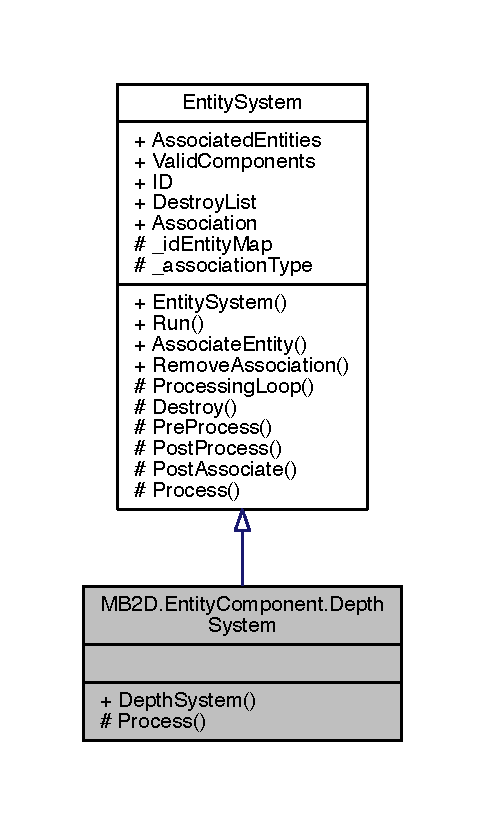
\includegraphics[width=233pt]{class_m_b2_d_1_1_entity_component_1_1_depth_system__inherit__graph}
\end{center}
\end{figure}


Collaboration diagram for M\+B2\+D.\+Entity\+Component.\+Depth\+System\+:
\nopagebreak
\begin{figure}[H]
\begin{center}
\leavevmode
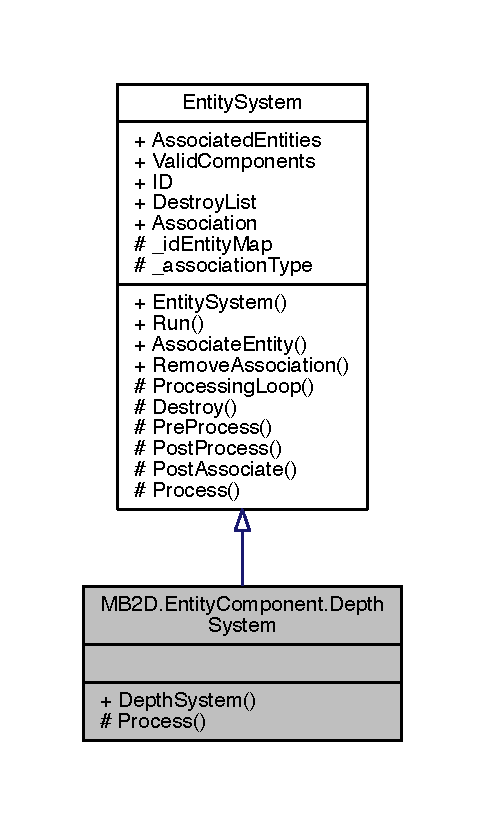
\includegraphics[width=233pt]{class_m_b2_d_1_1_entity_component_1_1_depth_system__coll__graph}
\end{center}
\end{figure}
\subsection*{Public Member Functions}
\begin{DoxyCompactItemize}
\item 
\hyperlink{class_m_b2_d_1_1_entity_component_1_1_depth_system_a5a7f2fc4d65f99bb89624cbcd1d52d65}{Depth\+System} ()
\begin{DoxyCompactList}\small\item\em Initializes a new instance of the T\+:\+M\+B2\+D.\+Entity\+Component.\+Depth\+System class. \end{DoxyCompactList}\end{DoxyCompactItemize}
\subsection*{Protected Member Functions}
\begin{DoxyCompactItemize}
\item 
override void \hyperlink{class_m_b2_d_1_1_entity_component_1_1_depth_system_a738556bdf819c9c0d4082a323a502c58}{Process} (\hyperlink{class_m_b2_d_1_1_entity_component_1_1_entity}{Entity} entity)
\begin{DoxyCompactList}\small\item\em Changes the z index based on the y coordinate of the entities bounds top \end{DoxyCompactList}\end{DoxyCompactItemize}
\subsection*{Additional Inherited Members}


\subsection{Detailed Description}
Changes an entities z-\/index based on the y coordinate of the top of their sprite 



\subsection{Constructor \& Destructor Documentation}
\hypertarget{class_m_b2_d_1_1_entity_component_1_1_depth_system_a5a7f2fc4d65f99bb89624cbcd1d52d65}{}\label{class_m_b2_d_1_1_entity_component_1_1_depth_system_a5a7f2fc4d65f99bb89624cbcd1d52d65} 
\index{M\+B2\+D\+::\+Entity\+Component\+::\+Depth\+System@{M\+B2\+D\+::\+Entity\+Component\+::\+Depth\+System}!Depth\+System@{Depth\+System}}
\index{Depth\+System@{Depth\+System}!M\+B2\+D\+::\+Entity\+Component\+::\+Depth\+System@{M\+B2\+D\+::\+Entity\+Component\+::\+Depth\+System}}
\subsubsection{\texorpdfstring{Depth\+System()}{DepthSystem()}}
{\footnotesize\ttfamily M\+B2\+D.\+Entity\+Component.\+Depth\+System.\+Depth\+System (\begin{DoxyParamCaption}{ }\end{DoxyParamCaption})\hspace{0.3cm}{\ttfamily [inline]}}



Initializes a new instance of the T\+:\+M\+B2\+D.\+Entity\+Component.\+Depth\+System class. 



\subsection{Member Function Documentation}
\hypertarget{class_m_b2_d_1_1_entity_component_1_1_depth_system_a738556bdf819c9c0d4082a323a502c58}{}\label{class_m_b2_d_1_1_entity_component_1_1_depth_system_a738556bdf819c9c0d4082a323a502c58} 
\index{M\+B2\+D\+::\+Entity\+Component\+::\+Depth\+System@{M\+B2\+D\+::\+Entity\+Component\+::\+Depth\+System}!Process@{Process}}
\index{Process@{Process}!M\+B2\+D\+::\+Entity\+Component\+::\+Depth\+System@{M\+B2\+D\+::\+Entity\+Component\+::\+Depth\+System}}
\subsubsection{\texorpdfstring{Process()}{Process()}}
{\footnotesize\ttfamily override void M\+B2\+D.\+Entity\+Component.\+Depth\+System.\+Process (\begin{DoxyParamCaption}\item[{\hyperlink{class_m_b2_d_1_1_entity_component_1_1_entity}{Entity}}]{entity }\end{DoxyParamCaption})\hspace{0.3cm}{\ttfamily [inline]}, {\ttfamily [protected]}, {\ttfamily [virtual]}}



Changes the z index based on the y coordinate of the entities bounds top 


\begin{DoxyParams}{Parameters}
{\em entity} & \hyperlink{class_m_b2_d_1_1_entity_component_1_1_entity}{Entity} to process.\\
\hline
\end{DoxyParams}


Implements \hyperlink{class_m_b2_d_1_1_entity_component_1_1_entity_system_abbf83b87cb5d12754fb058cef50451fa}{M\+B2\+D.\+Entity\+Component.\+Entity\+System}.



The documentation for this class was generated from the following file\+:\begin{DoxyCompactItemize}
\item 
M\+B2\+D/src/\+Entity\+Component/\+Systems/Depth\+System.\+cs\end{DoxyCompactItemize}

\hypertarget{class_m_b2_d_1_1_entity_component_1_1_entity}{}\section{M\+B2\+D.\+Entity\+Component.\+Entity Class Reference}
\label{class_m_b2_d_1_1_entity_component_1_1_entity}\index{M\+B2\+D.\+Entity\+Component.\+Entity@{M\+B2\+D.\+Entity\+Component.\+Entity}}


Represents a tagged and id\textquotesingle{}d container for components that can be operated on by systems.  




Collaboration diagram for M\+B2\+D.\+Entity\+Component.\+Entity\+:\nopagebreak
\begin{figure}[H]
\begin{center}
\leavevmode
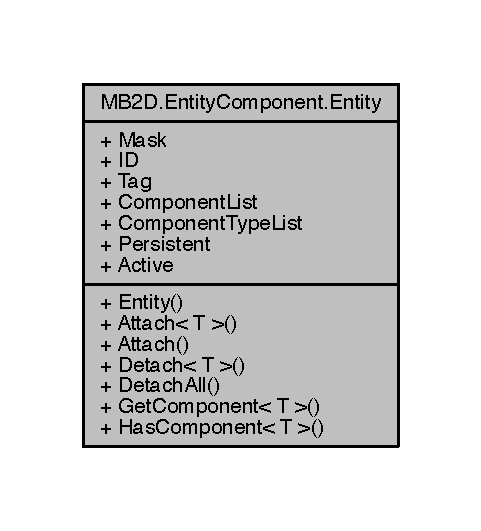
\includegraphics[width=231pt]{class_m_b2_d_1_1_entity_component_1_1_entity__coll__graph}
\end{center}
\end{figure}
\subsection*{Public Member Functions}
\begin{DoxyCompactItemize}
\item 
\hyperlink{class_m_b2_d_1_1_entity_component_1_1_entity_a6decb855bea1bcf18cd6c2869ebc16a6}{Entity} (\hyperlink{class_m_b2_d_1_1_entity_component_1_1_entity_map}{Entity\+Map} container, string tag=\char`\"{}\char`\"{})
\begin{DoxyCompactList}\small\item\em Initializes a new instance of the T\+:\+M\+B2\+D.\+Entity\+Component.\+Entity class. \end{DoxyCompactList}\item 
\hyperlink{interface_m_b2_d_1_1_entity_component_1_1_i_component}{I\+Component} \hyperlink{class_m_b2_d_1_1_entity_component_1_1_entity_a53ffea8d43423903712540fc2df6b82d}{Attach$<$ T $>$} (params object\mbox{[}$\,$\mbox{]} args)
\begin{DoxyCompactList}\small\item\em Attaches a new component to the entity. \end{DoxyCompactList}\item 
void \hyperlink{class_m_b2_d_1_1_entity_component_1_1_entity_aa86d1be62df6d89b981d1000c856a306}{Attach} (\hyperlink{interface_m_b2_d_1_1_entity_component_1_1_i_component}{I\+Component} component)
\begin{DoxyCompactList}\small\item\em Attaches a new component to the entity. \end{DoxyCompactList}\item 
void \hyperlink{class_m_b2_d_1_1_entity_component_1_1_entity_a9194f3b1f3370d2ecb47efe077ba4050}{Detach$<$ T $>$} ()
\begin{DoxyCompactList}\small\item\em Detatches a specific component from the entity \end{DoxyCompactList}\item 
void \hyperlink{class_m_b2_d_1_1_entity_component_1_1_entity_a5c006a368383ba7b17653d9f958ceaf8}{Detach\+All} ()
\begin{DoxyCompactList}\small\item\em Detachs all of the entities attached components. \end{DoxyCompactList}\item 
T \hyperlink{class_m_b2_d_1_1_entity_component_1_1_entity_a637f3b4df5ecd5d4e6c7630740d1676f}{Get\+Component$<$ T $>$} ()
\begin{DoxyCompactList}\small\item\em Queries the entity to see if it has a component attached and returns it if it does \end{DoxyCompactList}\item 
bool \hyperlink{class_m_b2_d_1_1_entity_component_1_1_entity_a8bbe196918b2eb4fe2102285c310ced3}{Has\+Component$<$ T $>$} ()
\begin{DoxyCompactList}\small\item\em Checks if an entity has a specific component attached \end{DoxyCompactList}\end{DoxyCompactItemize}
\subsection*{Properties}
\begin{DoxyCompactItemize}
\item 
ulong \hyperlink{class_m_b2_d_1_1_entity_component_1_1_entity_ada6cfb14adbc299a3b5616f833e4eb46}{Mask}\hspace{0.3cm}{\ttfamily  \mbox{[}get, set\mbox{]}}
\begin{DoxyCompactList}\small\item\em Gets and sets the entities component mask. \end{DoxyCompactList}\item 
ulong \hyperlink{class_m_b2_d_1_1_entity_component_1_1_entity_a915dff6f7cff6dbf93377df68fab7c0e}{ID}\hspace{0.3cm}{\ttfamily  \mbox{[}get, set\mbox{]}}
\begin{DoxyCompactList}\small\item\em Gets and sets the entities Globally Unique ID in the \hyperlink{class_m_b2_d_1_1_entity_component_1_1_entity_map}{Entity\+Map} \end{DoxyCompactList}\item 
string \hyperlink{class_m_b2_d_1_1_entity_component_1_1_entity_aa16727c7f2228b661fe6b374721fb4f7}{Tag}\hspace{0.3cm}{\ttfamily  \mbox{[}get\mbox{]}}
\begin{DoxyCompactList}\small\item\em Gets this entities tagname \end{DoxyCompactList}\item 
Dictionary$<$ Type, \hyperlink{interface_m_b2_d_1_1_entity_component_1_1_i_component}{I\+Component} $>$.Value\+Collection \hyperlink{class_m_b2_d_1_1_entity_component_1_1_entity_ae15b38df98affb3a58dc53c4a1140f3e}{Component\+List}\hspace{0.3cm}{\ttfamily  \mbox{[}get\mbox{]}}
\begin{DoxyCompactList}\small\item\em Gets the list if components attached to this entity. \end{DoxyCompactList}\item 
Dictionary$<$ Type, \hyperlink{interface_m_b2_d_1_1_entity_component_1_1_i_component}{I\+Component} $>$.Key\+Collection \hyperlink{class_m_b2_d_1_1_entity_component_1_1_entity_abd8ccf1511e8c825ee2574b3bc7af158}{Component\+Type\+List}\hspace{0.3cm}{\ttfamily  \mbox{[}get\mbox{]}}
\begin{DoxyCompactList}\small\item\em Gets the types of components this entity has attached \end{DoxyCompactList}\item 
bool \hyperlink{class_m_b2_d_1_1_entity_component_1_1_entity_af72e02dfa9b3b5a24e7c97eb6ce2fd3a}{Persistent}\hspace{0.3cm}{\ttfamily  \mbox{[}get, set\mbox{]}}
\begin{DoxyCompactList}\small\item\em Gets or sets a value indicating whether this T\+:\+M\+B2\+D.\+Entity\+Component.\+Entity is persistant in its parent T\+:\+M\+B2\+D.\+Entity\+Component.\+Entity\+Map. \end{DoxyCompactList}\item 
bool \hyperlink{class_m_b2_d_1_1_entity_component_1_1_entity_a3860df1e77b87727abd227e9e713a97b}{Active}\hspace{0.3cm}{\ttfamily  \mbox{[}get, set\mbox{]}}
\begin{DoxyCompactList}\small\item\em Gets or sets a value indicating whether this T\+:\+M\+B2\+D.\+Entity\+Component.\+Entity is active. Inactive entities are skipped over in each Entity\+Systems Process() method but aren\textquotesingle{}t destroyed. Allowing semi-\/persistant entities. \end{DoxyCompactList}\end{DoxyCompactItemize}


\subsection{Detailed Description}
Represents a tagged and id\textquotesingle{}d container for components that can be operated on by systems. 



\subsection{Constructor \& Destructor Documentation}
\hypertarget{class_m_b2_d_1_1_entity_component_1_1_entity_a6decb855bea1bcf18cd6c2869ebc16a6}{}\label{class_m_b2_d_1_1_entity_component_1_1_entity_a6decb855bea1bcf18cd6c2869ebc16a6} 
\index{M\+B2\+D\+::\+Entity\+Component\+::\+Entity@{M\+B2\+D\+::\+Entity\+Component\+::\+Entity}!Entity@{Entity}}
\index{Entity@{Entity}!M\+B2\+D\+::\+Entity\+Component\+::\+Entity@{M\+B2\+D\+::\+Entity\+Component\+::\+Entity}}
\subsubsection{\texorpdfstring{Entity()}{Entity()}}
{\footnotesize\ttfamily M\+B2\+D.\+Entity\+Component.\+Entity.\+Entity (\begin{DoxyParamCaption}\item[{\hyperlink{class_m_b2_d_1_1_entity_component_1_1_entity_map}{Entity\+Map}}]{container,  }\item[{string}]{tag = {\ttfamily \char`\"{}\char`\"{}} }\end{DoxyParamCaption})\hspace{0.3cm}{\ttfamily [inline]}}



Initializes a new instance of the T\+:\+M\+B2\+D.\+Entity\+Component.\+Entity class. 


\begin{DoxyParams}{Parameters}
{\em container} & The entities parent \hyperlink{class_m_b2_d_1_1_entity_component_1_1_entity_map}{Entity\+Map}\\
\hline
{\em tag} & Tagname to give the entity\\
\hline
\end{DoxyParams}


\subsection{Member Function Documentation}
\hypertarget{class_m_b2_d_1_1_entity_component_1_1_entity_aa86d1be62df6d89b981d1000c856a306}{}\label{class_m_b2_d_1_1_entity_component_1_1_entity_aa86d1be62df6d89b981d1000c856a306} 
\index{M\+B2\+D\+::\+Entity\+Component\+::\+Entity@{M\+B2\+D\+::\+Entity\+Component\+::\+Entity}!Attach@{Attach}}
\index{Attach@{Attach}!M\+B2\+D\+::\+Entity\+Component\+::\+Entity@{M\+B2\+D\+::\+Entity\+Component\+::\+Entity}}
\subsubsection{\texorpdfstring{Attach()}{Attach()}}
{\footnotesize\ttfamily void M\+B2\+D.\+Entity\+Component.\+Entity.\+Attach (\begin{DoxyParamCaption}\item[{\hyperlink{interface_m_b2_d_1_1_entity_component_1_1_i_component}{I\+Component}}]{component }\end{DoxyParamCaption})\hspace{0.3cm}{\ttfamily [inline]}}



Attaches a new component to the entity. 


\begin{DoxyParams}{Parameters}
{\em component} & Pre constructed component to add\\
\hline
\end{DoxyParams}
Here is the call graph for this function\+:\nopagebreak
\begin{figure}[H]
\begin{center}
\leavevmode
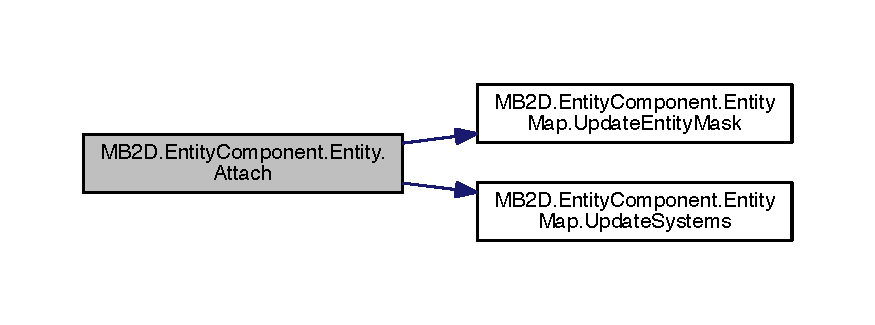
\includegraphics[width=350pt]{class_m_b2_d_1_1_entity_component_1_1_entity_aa86d1be62df6d89b981d1000c856a306_cgraph}
\end{center}
\end{figure}
Here is the caller graph for this function\+:\nopagebreak
\begin{figure}[H]
\begin{center}
\leavevmode
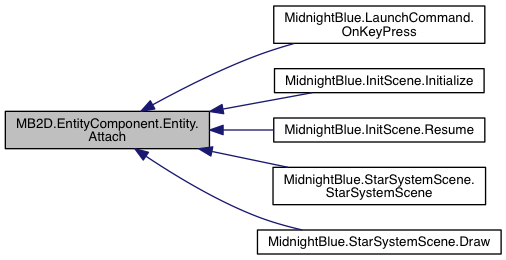
\includegraphics[width=350pt]{class_m_b2_d_1_1_entity_component_1_1_entity_aa86d1be62df6d89b981d1000c856a306_icgraph}
\end{center}
\end{figure}
\hypertarget{class_m_b2_d_1_1_entity_component_1_1_entity_a53ffea8d43423903712540fc2df6b82d}{}\label{class_m_b2_d_1_1_entity_component_1_1_entity_a53ffea8d43423903712540fc2df6b82d} 
\index{M\+B2\+D\+::\+Entity\+Component\+::\+Entity@{M\+B2\+D\+::\+Entity\+Component\+::\+Entity}!Attach$<$ T $>$@{Attach$<$ T $>$}}
\index{Attach$<$ T $>$@{Attach$<$ T $>$}!M\+B2\+D\+::\+Entity\+Component\+::\+Entity@{M\+B2\+D\+::\+Entity\+Component\+::\+Entity}}
\subsubsection{\texorpdfstring{Attach$<$ T $>$()}{Attach< T >()}}
{\footnotesize\ttfamily \hyperlink{interface_m_b2_d_1_1_entity_component_1_1_i_component}{I\+Component} \hyperlink{class_m_b2_d_1_1_entity_component_1_1_entity_aa86d1be62df6d89b981d1000c856a306}{M\+B2\+D.\+Entity\+Component.\+Entity.\+Attach}$<$ T $>$ (\begin{DoxyParamCaption}\item[{params object \mbox{[}$\,$\mbox{]}}]{args }\end{DoxyParamCaption})\hspace{0.3cm}{\ttfamily [inline]}}



Attaches a new component to the entity. 


\begin{DoxyParams}{Parameters}
{\em args} & The components constructor arguments\\
\hline
\end{DoxyParams}

\begin{DoxyTemplParams}{Template Parameters}
{\em T} & Type of component to attach\\
\hline
\end{DoxyTemplParams}
\begin{Desc}
\item[Type Constraints]\begin{description}
\item[{\em T} : {\em I\+Component}]\end{description}
\end{Desc}
Here is the call graph for this function\+:\nopagebreak
\begin{figure}[H]
\begin{center}
\leavevmode
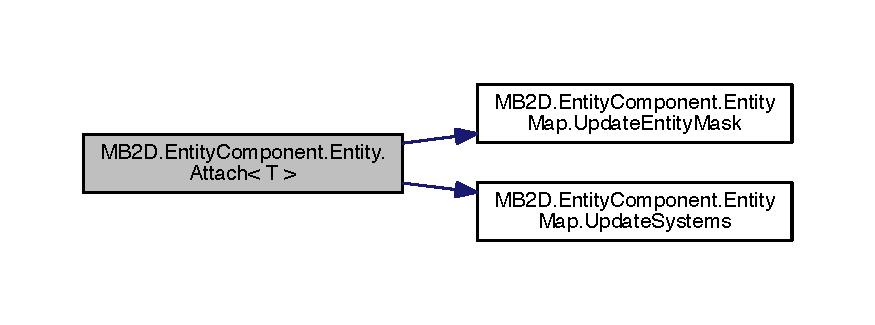
\includegraphics[width=350pt]{class_m_b2_d_1_1_entity_component_1_1_entity_a53ffea8d43423903712540fc2df6b82d_cgraph}
\end{center}
\end{figure}
\hypertarget{class_m_b2_d_1_1_entity_component_1_1_entity_a9194f3b1f3370d2ecb47efe077ba4050}{}\label{class_m_b2_d_1_1_entity_component_1_1_entity_a9194f3b1f3370d2ecb47efe077ba4050} 
\index{M\+B2\+D\+::\+Entity\+Component\+::\+Entity@{M\+B2\+D\+::\+Entity\+Component\+::\+Entity}!Detach$<$ T $>$@{Detach$<$ T $>$}}
\index{Detach$<$ T $>$@{Detach$<$ T $>$}!M\+B2\+D\+::\+Entity\+Component\+::\+Entity@{M\+B2\+D\+::\+Entity\+Component\+::\+Entity}}
\subsubsection{\texorpdfstring{Detach$<$ T $>$()}{Detach< T >()}}
{\footnotesize\ttfamily void M\+B2\+D.\+Entity\+Component.\+Entity.\+Detach$<$ T $>$ (\begin{DoxyParamCaption}{ }\end{DoxyParamCaption})\hspace{0.3cm}{\ttfamily [inline]}}



Detatches a specific component from the entity 


\begin{DoxyTemplParams}{Template Parameters}
{\em T} & The type of component to detatch.\\
\hline
\end{DoxyTemplParams}
\begin{Desc}
\item[Type Constraints]\begin{description}
\item[{\em T} : {\em I\+Component}]\end{description}
\end{Desc}
Here is the call graph for this function\+:\nopagebreak
\begin{figure}[H]
\begin{center}
\leavevmode
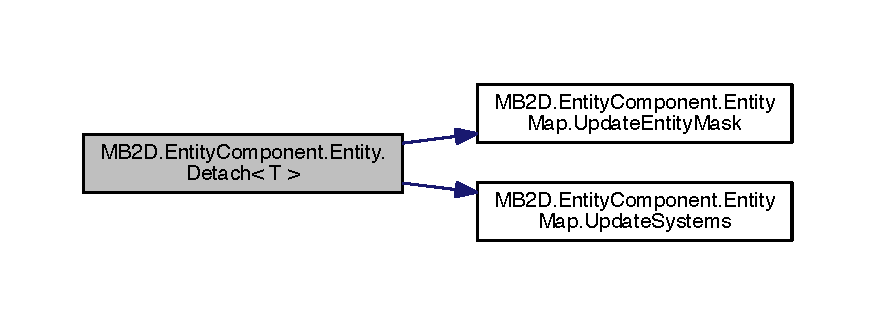
\includegraphics[width=350pt]{class_m_b2_d_1_1_entity_component_1_1_entity_a9194f3b1f3370d2ecb47efe077ba4050_cgraph}
\end{center}
\end{figure}
\hypertarget{class_m_b2_d_1_1_entity_component_1_1_entity_a5c006a368383ba7b17653d9f958ceaf8}{}\label{class_m_b2_d_1_1_entity_component_1_1_entity_a5c006a368383ba7b17653d9f958ceaf8} 
\index{M\+B2\+D\+::\+Entity\+Component\+::\+Entity@{M\+B2\+D\+::\+Entity\+Component\+::\+Entity}!Detach\+All@{Detach\+All}}
\index{Detach\+All@{Detach\+All}!M\+B2\+D\+::\+Entity\+Component\+::\+Entity@{M\+B2\+D\+::\+Entity\+Component\+::\+Entity}}
\subsubsection{\texorpdfstring{Detach\+All()}{DetachAll()}}
{\footnotesize\ttfamily void M\+B2\+D.\+Entity\+Component.\+Entity.\+Detach\+All (\begin{DoxyParamCaption}{ }\end{DoxyParamCaption})\hspace{0.3cm}{\ttfamily [inline]}}



Detachs all of the entities attached components. 

Here is the call graph for this function\+:\nopagebreak
\begin{figure}[H]
\begin{center}
\leavevmode
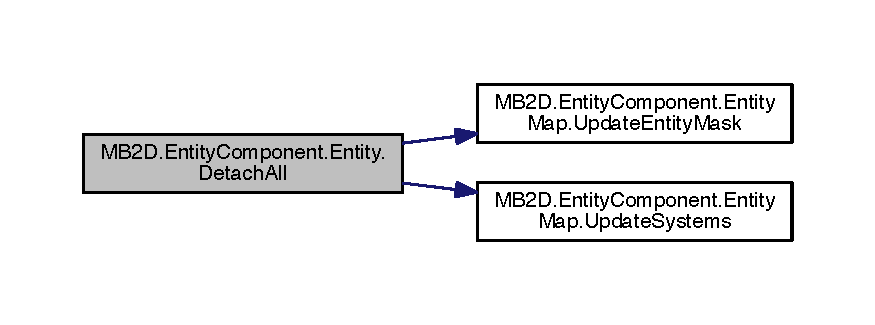
\includegraphics[width=350pt]{class_m_b2_d_1_1_entity_component_1_1_entity_a5c006a368383ba7b17653d9f958ceaf8_cgraph}
\end{center}
\end{figure}
Here is the caller graph for this function\+:\nopagebreak
\begin{figure}[H]
\begin{center}
\leavevmode
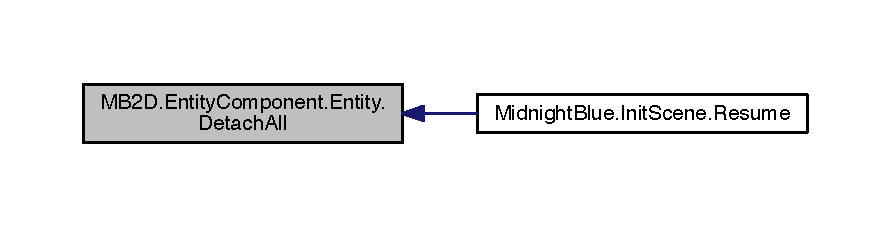
\includegraphics[width=350pt]{class_m_b2_d_1_1_entity_component_1_1_entity_a5c006a368383ba7b17653d9f958ceaf8_icgraph}
\end{center}
\end{figure}
\hypertarget{class_m_b2_d_1_1_entity_component_1_1_entity_a637f3b4df5ecd5d4e6c7630740d1676f}{}\label{class_m_b2_d_1_1_entity_component_1_1_entity_a637f3b4df5ecd5d4e6c7630740d1676f} 
\index{M\+B2\+D\+::\+Entity\+Component\+::\+Entity@{M\+B2\+D\+::\+Entity\+Component\+::\+Entity}!Get\+Component$<$ T $>$@{Get\+Component$<$ T $>$}}
\index{Get\+Component$<$ T $>$@{Get\+Component$<$ T $>$}!M\+B2\+D\+::\+Entity\+Component\+::\+Entity@{M\+B2\+D\+::\+Entity\+Component\+::\+Entity}}
\subsubsection{\texorpdfstring{Get\+Component$<$ T $>$()}{GetComponent< T >()}}
{\footnotesize\ttfamily T M\+B2\+D.\+Entity\+Component.\+Entity.\+Get\+Component$<$ T $>$ (\begin{DoxyParamCaption}{ }\end{DoxyParamCaption})\hspace{0.3cm}{\ttfamily [inline]}}



Queries the entity to see if it has a component attached and returns it if it does 

\begin{DoxyReturn}{Returns}
The component if the entity has it attached, null otherwise
\end{DoxyReturn}

\begin{DoxyTemplParams}{Template Parameters}
{\em T} & Component to query the entity for.\\
\hline
\end{DoxyTemplParams}
\begin{Desc}
\item[Type Constraints]\begin{description}
\item[{\em T} : {\em I\+Component}]\end{description}
\end{Desc}
\hypertarget{class_m_b2_d_1_1_entity_component_1_1_entity_a8bbe196918b2eb4fe2102285c310ced3}{}\label{class_m_b2_d_1_1_entity_component_1_1_entity_a8bbe196918b2eb4fe2102285c310ced3} 
\index{M\+B2\+D\+::\+Entity\+Component\+::\+Entity@{M\+B2\+D\+::\+Entity\+Component\+::\+Entity}!Has\+Component$<$ T $>$@{Has\+Component$<$ T $>$}}
\index{Has\+Component$<$ T $>$@{Has\+Component$<$ T $>$}!M\+B2\+D\+::\+Entity\+Component\+::\+Entity@{M\+B2\+D\+::\+Entity\+Component\+::\+Entity}}
\subsubsection{\texorpdfstring{Has\+Component$<$ T $>$()}{HasComponent< T >()}}
{\footnotesize\ttfamily bool M\+B2\+D.\+Entity\+Component.\+Entity.\+Has\+Component$<$ T $>$ (\begin{DoxyParamCaption}{ }\end{DoxyParamCaption})\hspace{0.3cm}{\ttfamily [inline]}}



Checks if an entity has a specific component attached 

\begin{DoxyReturn}{Returns}
{\ttfamily true}, if component is attached, {\ttfamily false} otherwise.
\end{DoxyReturn}

\begin{DoxyTemplParams}{Template Parameters}
{\em T} & The type of component to check.\\
\hline
\end{DoxyTemplParams}
\begin{Desc}
\item[Type Constraints]\begin{description}
\item[{\em T} : {\em I\+Component}]\end{description}
\end{Desc}


\subsection{Property Documentation}
\hypertarget{class_m_b2_d_1_1_entity_component_1_1_entity_a3860df1e77b87727abd227e9e713a97b}{}\label{class_m_b2_d_1_1_entity_component_1_1_entity_a3860df1e77b87727abd227e9e713a97b} 
\index{M\+B2\+D\+::\+Entity\+Component\+::\+Entity@{M\+B2\+D\+::\+Entity\+Component\+::\+Entity}!Active@{Active}}
\index{Active@{Active}!M\+B2\+D\+::\+Entity\+Component\+::\+Entity@{M\+B2\+D\+::\+Entity\+Component\+::\+Entity}}
\subsubsection{\texorpdfstring{Active}{Active}}
{\footnotesize\ttfamily bool M\+B2\+D.\+Entity\+Component.\+Entity.\+Active\hspace{0.3cm}{\ttfamily [get]}, {\ttfamily [set]}}



Gets or sets a value indicating whether this T\+:\+M\+B2\+D.\+Entity\+Component.\+Entity is active. Inactive entities are skipped over in each Entity\+Systems Process() method but aren\textquotesingle{}t destroyed. Allowing semi-\/persistant entities. 

{\ttfamily true} if the entity is active; otherwise, {\ttfamily false}.\hypertarget{class_m_b2_d_1_1_entity_component_1_1_entity_ae15b38df98affb3a58dc53c4a1140f3e}{}\label{class_m_b2_d_1_1_entity_component_1_1_entity_ae15b38df98affb3a58dc53c4a1140f3e} 
\index{M\+B2\+D\+::\+Entity\+Component\+::\+Entity@{M\+B2\+D\+::\+Entity\+Component\+::\+Entity}!Component\+List@{Component\+List}}
\index{Component\+List@{Component\+List}!M\+B2\+D\+::\+Entity\+Component\+::\+Entity@{M\+B2\+D\+::\+Entity\+Component\+::\+Entity}}
\subsubsection{\texorpdfstring{Component\+List}{ComponentList}}
{\footnotesize\ttfamily Dictionary$<$Type, \hyperlink{interface_m_b2_d_1_1_entity_component_1_1_i_component}{I\+Component}$>$.Value\+Collection M\+B2\+D.\+Entity\+Component.\+Entity.\+Component\+List\hspace{0.3cm}{\ttfamily [get]}}



Gets the list if components attached to this entity. 

The component list.\hypertarget{class_m_b2_d_1_1_entity_component_1_1_entity_abd8ccf1511e8c825ee2574b3bc7af158}{}\label{class_m_b2_d_1_1_entity_component_1_1_entity_abd8ccf1511e8c825ee2574b3bc7af158} 
\index{M\+B2\+D\+::\+Entity\+Component\+::\+Entity@{M\+B2\+D\+::\+Entity\+Component\+::\+Entity}!Component\+Type\+List@{Component\+Type\+List}}
\index{Component\+Type\+List@{Component\+Type\+List}!M\+B2\+D\+::\+Entity\+Component\+::\+Entity@{M\+B2\+D\+::\+Entity\+Component\+::\+Entity}}
\subsubsection{\texorpdfstring{Component\+Type\+List}{ComponentTypeList}}
{\footnotesize\ttfamily Dictionary$<$Type, \hyperlink{interface_m_b2_d_1_1_entity_component_1_1_i_component}{I\+Component}$>$.Key\+Collection M\+B2\+D.\+Entity\+Component.\+Entity.\+Component\+Type\+List\hspace{0.3cm}{\ttfamily [get]}}



Gets the types of components this entity has attached 

The component type list.\hypertarget{class_m_b2_d_1_1_entity_component_1_1_entity_a915dff6f7cff6dbf93377df68fab7c0e}{}\label{class_m_b2_d_1_1_entity_component_1_1_entity_a915dff6f7cff6dbf93377df68fab7c0e} 
\index{M\+B2\+D\+::\+Entity\+Component\+::\+Entity@{M\+B2\+D\+::\+Entity\+Component\+::\+Entity}!ID@{ID}}
\index{ID@{ID}!M\+B2\+D\+::\+Entity\+Component\+::\+Entity@{M\+B2\+D\+::\+Entity\+Component\+::\+Entity}}
\subsubsection{\texorpdfstring{ID}{ID}}
{\footnotesize\ttfamily ulong M\+B2\+D.\+Entity\+Component.\+Entity.\+ID\hspace{0.3cm}{\ttfamily [get]}, {\ttfamily [set]}}



Gets and sets the entities Globally Unique ID in the \hyperlink{class_m_b2_d_1_1_entity_component_1_1_entity_map}{Entity\+Map} 

G\+U\+ID\hypertarget{class_m_b2_d_1_1_entity_component_1_1_entity_ada6cfb14adbc299a3b5616f833e4eb46}{}\label{class_m_b2_d_1_1_entity_component_1_1_entity_ada6cfb14adbc299a3b5616f833e4eb46} 
\index{M\+B2\+D\+::\+Entity\+Component\+::\+Entity@{M\+B2\+D\+::\+Entity\+Component\+::\+Entity}!Mask@{Mask}}
\index{Mask@{Mask}!M\+B2\+D\+::\+Entity\+Component\+::\+Entity@{M\+B2\+D\+::\+Entity\+Component\+::\+Entity}}
\subsubsection{\texorpdfstring{Mask}{Mask}}
{\footnotesize\ttfamily ulong M\+B2\+D.\+Entity\+Component.\+Entity.\+Mask\hspace{0.3cm}{\ttfamily [get]}, {\ttfamily [set]}}



Gets and sets the entities component mask. 

The component mask.\hypertarget{class_m_b2_d_1_1_entity_component_1_1_entity_af72e02dfa9b3b5a24e7c97eb6ce2fd3a}{}\label{class_m_b2_d_1_1_entity_component_1_1_entity_af72e02dfa9b3b5a24e7c97eb6ce2fd3a} 
\index{M\+B2\+D\+::\+Entity\+Component\+::\+Entity@{M\+B2\+D\+::\+Entity\+Component\+::\+Entity}!Persistent@{Persistent}}
\index{Persistent@{Persistent}!M\+B2\+D\+::\+Entity\+Component\+::\+Entity@{M\+B2\+D\+::\+Entity\+Component\+::\+Entity}}
\subsubsection{\texorpdfstring{Persistent}{Persistent}}
{\footnotesize\ttfamily bool M\+B2\+D.\+Entity\+Component.\+Entity.\+Persistent\hspace{0.3cm}{\ttfamily [get]}, {\ttfamily [set]}}



Gets or sets a value indicating whether this T\+:\+M\+B2\+D.\+Entity\+Component.\+Entity is persistant in its parent T\+:\+M\+B2\+D.\+Entity\+Component.\+Entity\+Map. 

{\ttfamily true} if persistant; otherwise, {\ttfamily false}.\hypertarget{class_m_b2_d_1_1_entity_component_1_1_entity_aa16727c7f2228b661fe6b374721fb4f7}{}\label{class_m_b2_d_1_1_entity_component_1_1_entity_aa16727c7f2228b661fe6b374721fb4f7} 
\index{M\+B2\+D\+::\+Entity\+Component\+::\+Entity@{M\+B2\+D\+::\+Entity\+Component\+::\+Entity}!Tag@{Tag}}
\index{Tag@{Tag}!M\+B2\+D\+::\+Entity\+Component\+::\+Entity@{M\+B2\+D\+::\+Entity\+Component\+::\+Entity}}
\subsubsection{\texorpdfstring{Tag}{Tag}}
{\footnotesize\ttfamily string M\+B2\+D.\+Entity\+Component.\+Entity.\+Tag\hspace{0.3cm}{\ttfamily [get]}}



Gets this entities tagname 

The tagname

The documentation for this class was generated from the following file\+:\begin{DoxyCompactItemize}
\item 
M\+B2\+D/src/\+Entity\+Component/Entity.\+cs\end{DoxyCompactItemize}

\hypertarget{struct_m_b2_d_1_1_testing_1_1_entity_container_tests}{}\section{M\+B2\+D.\+Testing.\+Entity\+Container\+Tests Struct Reference}
\label{struct_m_b2_d_1_1_testing_1_1_entity_container_tests}\index{M\+B2\+D.\+Testing.\+Entity\+Container\+Tests@{M\+B2\+D.\+Testing.\+Entity\+Container\+Tests}}


Collaboration diagram for M\+B2\+D.\+Testing.\+Entity\+Container\+Tests\+:\nopagebreak
\begin{figure}[H]
\begin{center}
\leavevmode
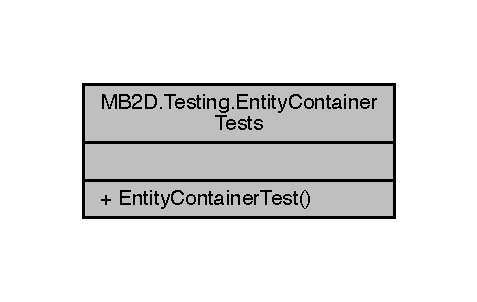
\includegraphics[width=229pt]{struct_m_b2_d_1_1_testing_1_1_entity_container_tests__coll__graph}
\end{center}
\end{figure}
\subsection*{Static Public Member Functions}
\begin{DoxyCompactItemize}
\item 
\hypertarget{struct_m_b2_d_1_1_testing_1_1_entity_container_tests_a745b6bc43f1feb392b1e835ee86acac0}{}\label{struct_m_b2_d_1_1_testing_1_1_entity_container_tests_a745b6bc43f1feb392b1e835ee86acac0} 
static void {\bfseries Entity\+Container\+Test} (params string\mbox{[}$\,$\mbox{]} args)
\end{DoxyCompactItemize}


The documentation for this struct was generated from the following file\+:\begin{DoxyCompactItemize}
\item 
M\+B2\+D/src/\+Test/Entity\+Container\+Tests.\+cs\end{DoxyCompactItemize}

\hypertarget{class_m_b2_d_1_1_entity_component_1_1_entity_map}{}\subsection{M\+B2\+D.\+Entity\+Component.\+Entity\+Map Class Reference}
\label{class_m_b2_d_1_1_entity_component_1_1_entity_map}\index{M\+B2\+D.\+Entity\+Component.\+Entity\+Map@{M\+B2\+D.\+Entity\+Component.\+Entity\+Map}}


Maps entities, systems and components to one another and provides querying and updating access to all elements  




Collaboration diagram for M\+B2\+D.\+Entity\+Component.\+Entity\+Map\+:
\nopagebreak
\begin{figure}[H]
\begin{center}
\leavevmode
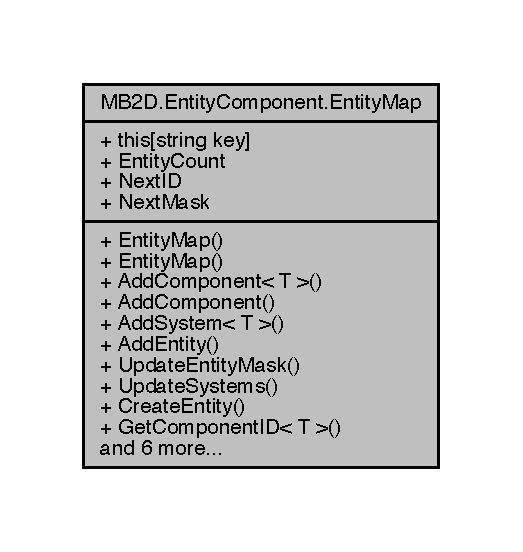
\includegraphics[width=251pt]{class_m_b2_d_1_1_entity_component_1_1_entity_map__coll__graph}
\end{center}
\end{figure}
\subsubsection*{Public Member Functions}
\begin{DoxyCompactItemize}
\item 
\hyperlink{class_m_b2_d_1_1_entity_component_1_1_entity_map_a3904c9181b806e476be24848837e1b53}{Entity\+Map} ()
\begin{DoxyCompactList}\small\item\em Initializes a new instance of the T\+:\+M\+B2\+D.\+Entity\+Component.\+Entity\+Map class. \end{DoxyCompactList}\item 
\hyperlink{class_m_b2_d_1_1_entity_component_1_1_entity_map_ac8f0662e42b90d8299e1044a1c429863}{Entity\+Map} (\hyperlink{class_m_b2_d_1_1_entity_component_1_1_entity_map}{Entity\+Map} map)
\begin{DoxyCompactList}\small\item\em Initializes a new instance of the T\+:\+M\+B2\+D.\+Entity\+Component.\+Entity\+Map class. Uses an existing \hyperlink{class_m_b2_d_1_1_entity_component_1_1_entity_map}{Entity\+Map} to copy all registered systems and components as well as any persistant Entities. \end{DoxyCompactList}\item 
void \hyperlink{class_m_b2_d_1_1_entity_component_1_1_entity_map_a3832e5a6ae181f71d002e81caf008da4}{Add\+Component$<$ T $>$} ()
\begin{DoxyCompactList}\small\item\em Registers a new component type to the \hyperlink{class_m_b2_d_1_1_entity_component_1_1_entity_map}{Entity\+Map} \end{DoxyCompactList}\item 
void \hyperlink{class_m_b2_d_1_1_entity_component_1_1_entity_map_aff9e50266b46d782c31c5b482b86540c}{Add\+Component} (Type component\+Type)
\begin{DoxyCompactList}\small\item\em Registers a new component type to the \hyperlink{class_m_b2_d_1_1_entity_component_1_1_entity_map}{Entity\+Map} \end{DoxyCompactList}\item 
void \hyperlink{class_m_b2_d_1_1_entity_component_1_1_entity_map_af2aefc425308f1ca680b0083f3acab0d}{Add\+System$<$ T $>$} (params object\mbox{[}$\,$\mbox{]} args)
\begin{DoxyCompactList}\small\item\em Registers a new \hyperlink{class_m_b2_d_1_1_entity_component_1_1_entity_system}{Entity\+System} to the map \end{DoxyCompactList}\item 
void \hyperlink{class_m_b2_d_1_1_entity_component_1_1_entity_map_a0800ef900f92c04902d5b1c355aab900}{Add\+Entity} (\hyperlink{class_m_b2_d_1_1_entity_component_1_1_entity}{Entity} entity)
\begin{DoxyCompactList}\small\item\em Adds a created entity to this map \end{DoxyCompactList}\item 
void \hyperlink{class_m_b2_d_1_1_entity_component_1_1_entity_map_a968ce46cbba14cdc7814dd308f133949}{Update\+Entity\+Mask} (\hyperlink{class_m_b2_d_1_1_entity_component_1_1_entity}{Entity} entity)
\begin{DoxyCompactList}\small\item\em Updates a specific entities component mask. Use after registering new components or systems. \end{DoxyCompactList}\item 
void \hyperlink{class_m_b2_d_1_1_entity_component_1_1_entity_map_ab6078e0b6eddb220b9bbf5d358d6e365}{Update\+Systems} (\hyperlink{class_m_b2_d_1_1_entity_component_1_1_entity}{Entity} entity)
\begin{DoxyCompactList}\small\item\em Updates each systems associated entity list, adding the specified \hyperlink{class_m_b2_d_1_1_entity_component_1_1_entity}{Entity}. Use after creating a new \hyperlink{class_m_b2_d_1_1_entity_component_1_1_entity}{Entity} and adding it manually \end{DoxyCompactList}\item 
\hyperlink{class_m_b2_d_1_1_entity_component_1_1_entity}{Entity} \hyperlink{class_m_b2_d_1_1_entity_component_1_1_entity_map_a2461bfeb368018daadb2578c445f8fc2}{Create\+Entity} (string tag=\char`\"{}\char`\"{})
\begin{DoxyCompactList}\small\item\em Creates a new \hyperlink{class_m_b2_d_1_1_entity_component_1_1_entity}{Entity} with the given tag in this map. Auto-\/\+Registers the entity with all systems and updates its mask. \end{DoxyCompactList}\item 
ulong \hyperlink{class_m_b2_d_1_1_entity_component_1_1_entity_map_ad0a7991327281d908b72b33bc1944b70}{Get\+Component\+I\+D$<$ T $>$} ()
\begin{DoxyCompactList}\small\item\em Gets the id of a specified component type if it exists. \end{DoxyCompactList}\item 
\hyperlink{class_m_b2_d_1_1_entity_component_1_1_entity_system}{Entity\+System} \hyperlink{class_m_b2_d_1_1_entity_component_1_1_entity_map_a1240739b3c9be7daeebd2a0ae3cc04ff}{Get\+System$<$ T $>$} ()
\begin{DoxyCompactList}\small\item\em Retrieves a pre-\/registered system from the map \end{DoxyCompactList}\item 
\hypertarget{class_m_b2_d_1_1_entity_component_1_1_entity_map_ab84f162ddcef10ea2076c23d99f8e40f}{}\label{class_m_b2_d_1_1_entity_component_1_1_entity_map_ab84f162ddcef10ea2076c23d99f8e40f} 
List$<$ \hyperlink{class_m_b2_d_1_1_entity_component_1_1_entity}{Entity} $>$ {\bfseries Entities\+With\+Component$<$ T $>$} ()
\item 
void \hyperlink{class_m_b2_d_1_1_entity_component_1_1_entity_map_a079e8e957e7fbaa8de73e609ab646fe1}{Clear} ()
\begin{DoxyCompactList}\small\item\em Clears all entities from this map except for any marked as persistant. \end{DoxyCompactList}\item 
\hypertarget{class_m_b2_d_1_1_entity_component_1_1_entity_map_a3d42b78583ee8cf16a9ce1c2d096ea01}{}\label{class_m_b2_d_1_1_entity_component_1_1_entity_map_a3d42b78583ee8cf16a9ce1c2d096ea01} 
void {\bfseries Reset} ()
\item 
\hypertarget{class_m_b2_d_1_1_entity_component_1_1_entity_map_ad796d08b2566bdfa3862e54ba639e3ae}{}\label{class_m_b2_d_1_1_entity_component_1_1_entity_map_ad796d08b2566bdfa3862e54ba639e3ae} 
void {\bfseries Make\+Blueprint} (string id, Action$<$ \hyperlink{class_m_b2_d_1_1_entity_component_1_1_entity}{Entity} $>$ build\+Function)
\item 
\hypertarget{class_m_b2_d_1_1_entity_component_1_1_entity_map_a11e3a65f0404ad99f2a1aff9b0604d15}{}\label{class_m_b2_d_1_1_entity_component_1_1_entity_map_a11e3a65f0404ad99f2a1aff9b0604d15} 
void {\bfseries Use\+Blueprint} (string name, \hyperlink{class_m_b2_d_1_1_entity_component_1_1_entity}{Entity} entity)
\end{DoxyCompactItemize}
\subsubsection*{Properties}
\begin{DoxyCompactItemize}
\item 
\hyperlink{class_m_b2_d_1_1_entity_component_1_1_entity}{Entity} \hyperlink{class_m_b2_d_1_1_entity_component_1_1_entity_map_ae29ad08673cc4c756b43bd3a72c35b84}{this\mbox{[}string key\mbox{]}}\hspace{0.3cm}{\ttfamily  \mbox{[}get\mbox{]}}
\begin{DoxyCompactList}\small\item\em Gets the T\+:\+M\+B2\+D.\+Entity\+Component.\+Entity with the specified tag if it exists; null otherwise \end{DoxyCompactList}\item 
int \hyperlink{class_m_b2_d_1_1_entity_component_1_1_entity_map_a607d25be9724ca759ecef96fe76ee516}{Entity\+Count}\hspace{0.3cm}{\ttfamily  \mbox{[}get\mbox{]}}
\begin{DoxyCompactList}\small\item\em Gets the number of entities in the map. \end{DoxyCompactList}\item 
ulong \hyperlink{class_m_b2_d_1_1_entity_component_1_1_entity_map_a812155313251122f297b6653ab4f4ec1}{Next\+ID}\hspace{0.3cm}{\ttfamily  \mbox{[}get\mbox{]}}
\begin{DoxyCompactList}\small\item\em Auto-\/increments the last generated G\+U\+ID and retrieves the result \end{DoxyCompactList}\end{DoxyCompactItemize}


\subsubsection{Detailed Description}
Maps entities, systems and components to one another and provides querying and updating access to all elements 



\subsubsection{Constructor \& Destructor Documentation}
\hypertarget{class_m_b2_d_1_1_entity_component_1_1_entity_map_a3904c9181b806e476be24848837e1b53}{}\label{class_m_b2_d_1_1_entity_component_1_1_entity_map_a3904c9181b806e476be24848837e1b53} 
\index{M\+B2\+D\+::\+Entity\+Component\+::\+Entity\+Map@{M\+B2\+D\+::\+Entity\+Component\+::\+Entity\+Map}!Entity\+Map@{Entity\+Map}}
\index{Entity\+Map@{Entity\+Map}!M\+B2\+D\+::\+Entity\+Component\+::\+Entity\+Map@{M\+B2\+D\+::\+Entity\+Component\+::\+Entity\+Map}}
\paragraph{\texorpdfstring{Entity\+Map()}{EntityMap()}\hspace{0.1cm}{\footnotesize\ttfamily [1/2]}}
{\footnotesize\ttfamily M\+B2\+D.\+Entity\+Component.\+Entity\+Map.\+Entity\+Map (\begin{DoxyParamCaption}{ }\end{DoxyParamCaption})\hspace{0.3cm}{\ttfamily [inline]}}



Initializes a new instance of the T\+:\+M\+B2\+D.\+Entity\+Component.\+Entity\+Map class. 

\hypertarget{class_m_b2_d_1_1_entity_component_1_1_entity_map_ac8f0662e42b90d8299e1044a1c429863}{}\label{class_m_b2_d_1_1_entity_component_1_1_entity_map_ac8f0662e42b90d8299e1044a1c429863} 
\index{M\+B2\+D\+::\+Entity\+Component\+::\+Entity\+Map@{M\+B2\+D\+::\+Entity\+Component\+::\+Entity\+Map}!Entity\+Map@{Entity\+Map}}
\index{Entity\+Map@{Entity\+Map}!M\+B2\+D\+::\+Entity\+Component\+::\+Entity\+Map@{M\+B2\+D\+::\+Entity\+Component\+::\+Entity\+Map}}
\paragraph{\texorpdfstring{Entity\+Map()}{EntityMap()}\hspace{0.1cm}{\footnotesize\ttfamily [2/2]}}
{\footnotesize\ttfamily M\+B2\+D.\+Entity\+Component.\+Entity\+Map.\+Entity\+Map (\begin{DoxyParamCaption}\item[{\hyperlink{class_m_b2_d_1_1_entity_component_1_1_entity_map}{Entity\+Map}}]{map }\end{DoxyParamCaption})\hspace{0.3cm}{\ttfamily [inline]}}



Initializes a new instance of the T\+:\+M\+B2\+D.\+Entity\+Component.\+Entity\+Map class. Uses an existing \hyperlink{class_m_b2_d_1_1_entity_component_1_1_entity_map}{Entity\+Map} to copy all registered systems and components as well as any persistant Entities. 


\begin{DoxyParams}{Parameters}
{\em map} & \hyperlink{class_m_b2_d_1_1_entity_component_1_1_entity_map}{Entity\+Map} to copy from\\
\hline
\end{DoxyParams}


\subsubsection{Member Function Documentation}
\hypertarget{class_m_b2_d_1_1_entity_component_1_1_entity_map_aff9e50266b46d782c31c5b482b86540c}{}\label{class_m_b2_d_1_1_entity_component_1_1_entity_map_aff9e50266b46d782c31c5b482b86540c} 
\index{M\+B2\+D\+::\+Entity\+Component\+::\+Entity\+Map@{M\+B2\+D\+::\+Entity\+Component\+::\+Entity\+Map}!Add\+Component@{Add\+Component}}
\index{Add\+Component@{Add\+Component}!M\+B2\+D\+::\+Entity\+Component\+::\+Entity\+Map@{M\+B2\+D\+::\+Entity\+Component\+::\+Entity\+Map}}
\paragraph{\texorpdfstring{Add\+Component()}{AddComponent()}}
{\footnotesize\ttfamily void M\+B2\+D.\+Entity\+Component.\+Entity\+Map.\+Add\+Component (\begin{DoxyParamCaption}\item[{Type}]{component\+Type }\end{DoxyParamCaption})\hspace{0.3cm}{\ttfamily [inline]}}



Registers a new component type to the \hyperlink{class_m_b2_d_1_1_entity_component_1_1_entity_map}{Entity\+Map} 


\begin{DoxyParams}{Parameters}
{\em component\+Type} & Type of component to register\\
\hline
\end{DoxyParams}
\hypertarget{class_m_b2_d_1_1_entity_component_1_1_entity_map_a3832e5a6ae181f71d002e81caf008da4}{}\label{class_m_b2_d_1_1_entity_component_1_1_entity_map_a3832e5a6ae181f71d002e81caf008da4} 
\index{M\+B2\+D\+::\+Entity\+Component\+::\+Entity\+Map@{M\+B2\+D\+::\+Entity\+Component\+::\+Entity\+Map}!Add\+Component$<$ T $>$@{Add\+Component$<$ T $>$}}
\index{Add\+Component$<$ T $>$@{Add\+Component$<$ T $>$}!M\+B2\+D\+::\+Entity\+Component\+::\+Entity\+Map@{M\+B2\+D\+::\+Entity\+Component\+::\+Entity\+Map}}
\paragraph{\texorpdfstring{Add\+Component$<$ T $>$()}{AddComponent< T >()}}
{\footnotesize\ttfamily void \hyperlink{class_m_b2_d_1_1_entity_component_1_1_entity_map_aff9e50266b46d782c31c5b482b86540c}{M\+B2\+D.\+Entity\+Component.\+Entity\+Map.\+Add\+Component}$<$ T $>$ (\begin{DoxyParamCaption}{ }\end{DoxyParamCaption})\hspace{0.3cm}{\ttfamily [inline]}}



Registers a new component type to the \hyperlink{class_m_b2_d_1_1_entity_component_1_1_entity_map}{Entity\+Map} 


\begin{DoxyTemplParams}{Template Parameters}
{\em T} & Type of component to register\\
\hline
\end{DoxyTemplParams}
\begin{Desc}
\item[Type Constraints]\begin{description}
\item[{\em T} : {\em I\+Component}]\end{description}
\end{Desc}
\hypertarget{class_m_b2_d_1_1_entity_component_1_1_entity_map_a0800ef900f92c04902d5b1c355aab900}{}\label{class_m_b2_d_1_1_entity_component_1_1_entity_map_a0800ef900f92c04902d5b1c355aab900} 
\index{M\+B2\+D\+::\+Entity\+Component\+::\+Entity\+Map@{M\+B2\+D\+::\+Entity\+Component\+::\+Entity\+Map}!Add\+Entity@{Add\+Entity}}
\index{Add\+Entity@{Add\+Entity}!M\+B2\+D\+::\+Entity\+Component\+::\+Entity\+Map@{M\+B2\+D\+::\+Entity\+Component\+::\+Entity\+Map}}
\paragraph{\texorpdfstring{Add\+Entity()}{AddEntity()}}
{\footnotesize\ttfamily void M\+B2\+D.\+Entity\+Component.\+Entity\+Map.\+Add\+Entity (\begin{DoxyParamCaption}\item[{\hyperlink{class_m_b2_d_1_1_entity_component_1_1_entity}{Entity}}]{entity }\end{DoxyParamCaption})\hspace{0.3cm}{\ttfamily [inline]}}



Adds a created entity to this map 


\begin{DoxyParams}{Parameters}
{\em entity} & \hyperlink{class_m_b2_d_1_1_entity_component_1_1_entity}{Entity} to add\\
\hline
\end{DoxyParams}
\hypertarget{class_m_b2_d_1_1_entity_component_1_1_entity_map_af2aefc425308f1ca680b0083f3acab0d}{}\label{class_m_b2_d_1_1_entity_component_1_1_entity_map_af2aefc425308f1ca680b0083f3acab0d} 
\index{M\+B2\+D\+::\+Entity\+Component\+::\+Entity\+Map@{M\+B2\+D\+::\+Entity\+Component\+::\+Entity\+Map}!Add\+System$<$ T $>$@{Add\+System$<$ T $>$}}
\index{Add\+System$<$ T $>$@{Add\+System$<$ T $>$}!M\+B2\+D\+::\+Entity\+Component\+::\+Entity\+Map@{M\+B2\+D\+::\+Entity\+Component\+::\+Entity\+Map}}
\paragraph{\texorpdfstring{Add\+System$<$ T $>$()}{AddSystem< T >()}}
{\footnotesize\ttfamily void M\+B2\+D.\+Entity\+Component.\+Entity\+Map.\+Add\+System$<$ T $>$ (\begin{DoxyParamCaption}\item[{params object \mbox{[}$\,$\mbox{]}}]{args }\end{DoxyParamCaption})\hspace{0.3cm}{\ttfamily [inline]}}



Registers a new \hyperlink{class_m_b2_d_1_1_entity_component_1_1_entity_system}{Entity\+System} to the map 


\begin{DoxyTemplParams}{Template Parameters}
{\em T} & \hyperlink{class_m_b2_d_1_1_entity_component_1_1_entity_system}{Entity\+System} type to add\\
\hline
\end{DoxyTemplParams}
\begin{Desc}
\item[Type Constraints]\begin{description}
\item[{\em T} : {\em Entity\+System}]\end{description}
\end{Desc}
\hypertarget{class_m_b2_d_1_1_entity_component_1_1_entity_map_a079e8e957e7fbaa8de73e609ab646fe1}{}\label{class_m_b2_d_1_1_entity_component_1_1_entity_map_a079e8e957e7fbaa8de73e609ab646fe1} 
\index{M\+B2\+D\+::\+Entity\+Component\+::\+Entity\+Map@{M\+B2\+D\+::\+Entity\+Component\+::\+Entity\+Map}!Clear@{Clear}}
\index{Clear@{Clear}!M\+B2\+D\+::\+Entity\+Component\+::\+Entity\+Map@{M\+B2\+D\+::\+Entity\+Component\+::\+Entity\+Map}}
\paragraph{\texorpdfstring{Clear()}{Clear()}}
{\footnotesize\ttfamily void M\+B2\+D.\+Entity\+Component.\+Entity\+Map.\+Clear (\begin{DoxyParamCaption}{ }\end{DoxyParamCaption})\hspace{0.3cm}{\ttfamily [inline]}}



Clears all entities from this map except for any marked as persistant. 

Here is the caller graph for this function\+:
\nopagebreak
\begin{figure}[H]
\begin{center}
\leavevmode
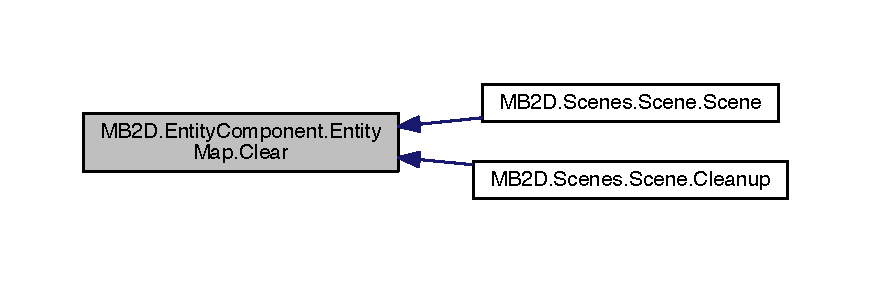
\includegraphics[width=350pt]{class_m_b2_d_1_1_entity_component_1_1_entity_map_a079e8e957e7fbaa8de73e609ab646fe1_icgraph}
\end{center}
\end{figure}
\hypertarget{class_m_b2_d_1_1_entity_component_1_1_entity_map_a2461bfeb368018daadb2578c445f8fc2}{}\label{class_m_b2_d_1_1_entity_component_1_1_entity_map_a2461bfeb368018daadb2578c445f8fc2} 
\index{M\+B2\+D\+::\+Entity\+Component\+::\+Entity\+Map@{M\+B2\+D\+::\+Entity\+Component\+::\+Entity\+Map}!Create\+Entity@{Create\+Entity}}
\index{Create\+Entity@{Create\+Entity}!M\+B2\+D\+::\+Entity\+Component\+::\+Entity\+Map@{M\+B2\+D\+::\+Entity\+Component\+::\+Entity\+Map}}
\paragraph{\texorpdfstring{Create\+Entity()}{CreateEntity()}}
{\footnotesize\ttfamily \hyperlink{class_m_b2_d_1_1_entity_component_1_1_entity}{Entity} M\+B2\+D.\+Entity\+Component.\+Entity\+Map.\+Create\+Entity (\begin{DoxyParamCaption}\item[{string}]{tag = {\ttfamily \char`\"{}\char`\"{}} }\end{DoxyParamCaption})\hspace{0.3cm}{\ttfamily [inline]}}



Creates a new \hyperlink{class_m_b2_d_1_1_entity_component_1_1_entity}{Entity} with the given tag in this map. Auto-\/\+Registers the entity with all systems and updates its mask. 

\begin{DoxyReturn}{Returns}
The created entity
\end{DoxyReturn}

\begin{DoxyParams}{Parameters}
{\em tag} & Tagname to give the entity\\
\hline
\end{DoxyParams}
\hypertarget{class_m_b2_d_1_1_entity_component_1_1_entity_map_ad0a7991327281d908b72b33bc1944b70}{}\label{class_m_b2_d_1_1_entity_component_1_1_entity_map_ad0a7991327281d908b72b33bc1944b70} 
\index{M\+B2\+D\+::\+Entity\+Component\+::\+Entity\+Map@{M\+B2\+D\+::\+Entity\+Component\+::\+Entity\+Map}!Get\+Component\+I\+D$<$ T $>$@{Get\+Component\+I\+D$<$ T $>$}}
\index{Get\+Component\+I\+D$<$ T $>$@{Get\+Component\+I\+D$<$ T $>$}!M\+B2\+D\+::\+Entity\+Component\+::\+Entity\+Map@{M\+B2\+D\+::\+Entity\+Component\+::\+Entity\+Map}}
\paragraph{\texorpdfstring{Get\+Component\+I\+D$<$ T $>$()}{GetComponentID< T >()}}
{\footnotesize\ttfamily ulong M\+B2\+D.\+Entity\+Component.\+Entity\+Map.\+Get\+Component\+ID$<$ T $>$ (\begin{DoxyParamCaption}{ }\end{DoxyParamCaption})\hspace{0.3cm}{\ttfamily [inline]}}



Gets the id of a specified component type if it exists. 

\begin{DoxyReturn}{Returns}
The component id mask.
\end{DoxyReturn}

\begin{DoxyTemplParams}{Template Parameters}
{\em T} & Type of component to query for.\\
\hline
\end{DoxyTemplParams}
\begin{Desc}
\item[Type Constraints]\begin{description}
\item[{\em T} : {\em I\+Component}]\end{description}
\end{Desc}
\hypertarget{class_m_b2_d_1_1_entity_component_1_1_entity_map_a1240739b3c9be7daeebd2a0ae3cc04ff}{}\label{class_m_b2_d_1_1_entity_component_1_1_entity_map_a1240739b3c9be7daeebd2a0ae3cc04ff} 
\index{M\+B2\+D\+::\+Entity\+Component\+::\+Entity\+Map@{M\+B2\+D\+::\+Entity\+Component\+::\+Entity\+Map}!Get\+System$<$ T $>$@{Get\+System$<$ T $>$}}
\index{Get\+System$<$ T $>$@{Get\+System$<$ T $>$}!M\+B2\+D\+::\+Entity\+Component\+::\+Entity\+Map@{M\+B2\+D\+::\+Entity\+Component\+::\+Entity\+Map}}
\paragraph{\texorpdfstring{Get\+System$<$ T $>$()}{GetSystem< T >()}}
{\footnotesize\ttfamily \hyperlink{class_m_b2_d_1_1_entity_component_1_1_entity_system}{Entity\+System} M\+B2\+D.\+Entity\+Component.\+Entity\+Map.\+Get\+System$<$ T $>$ (\begin{DoxyParamCaption}{ }\end{DoxyParamCaption})\hspace{0.3cm}{\ttfamily [inline]}}



Retrieves a pre-\/registered system from the map 

\begin{DoxyReturn}{Returns}
The system if it exists; null otherwise
\end{DoxyReturn}

\begin{DoxyTemplParams}{Template Parameters}
{\em T} & Type of system to retrieve.\\
\hline
\end{DoxyTemplParams}
\begin{Desc}
\item[Type Constraints]\begin{description}
\item[{\em T} : {\em Entity\+System}]\end{description}
\end{Desc}
\hypertarget{class_m_b2_d_1_1_entity_component_1_1_entity_map_a968ce46cbba14cdc7814dd308f133949}{}\label{class_m_b2_d_1_1_entity_component_1_1_entity_map_a968ce46cbba14cdc7814dd308f133949} 
\index{M\+B2\+D\+::\+Entity\+Component\+::\+Entity\+Map@{M\+B2\+D\+::\+Entity\+Component\+::\+Entity\+Map}!Update\+Entity\+Mask@{Update\+Entity\+Mask}}
\index{Update\+Entity\+Mask@{Update\+Entity\+Mask}!M\+B2\+D\+::\+Entity\+Component\+::\+Entity\+Map@{M\+B2\+D\+::\+Entity\+Component\+::\+Entity\+Map}}
\paragraph{\texorpdfstring{Update\+Entity\+Mask()}{UpdateEntityMask()}}
{\footnotesize\ttfamily void M\+B2\+D.\+Entity\+Component.\+Entity\+Map.\+Update\+Entity\+Mask (\begin{DoxyParamCaption}\item[{\hyperlink{class_m_b2_d_1_1_entity_component_1_1_entity}{Entity}}]{entity }\end{DoxyParamCaption})\hspace{0.3cm}{\ttfamily [inline]}}



Updates a specific entities component mask. Use after registering new components or systems. 


\begin{DoxyParams}{Parameters}
{\em entity} & \hyperlink{class_m_b2_d_1_1_entity_component_1_1_entity}{Entity} to update\\
\hline
\end{DoxyParams}
Here is the caller graph for this function\+:
\nopagebreak
\begin{figure}[H]
\begin{center}
\leavevmode
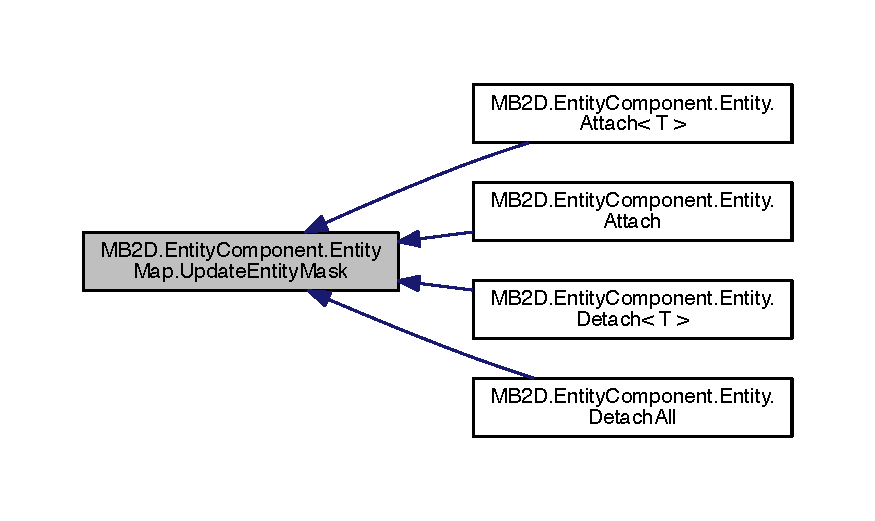
\includegraphics[width=350pt]{class_m_b2_d_1_1_entity_component_1_1_entity_map_a968ce46cbba14cdc7814dd308f133949_icgraph}
\end{center}
\end{figure}
\hypertarget{class_m_b2_d_1_1_entity_component_1_1_entity_map_ab6078e0b6eddb220b9bbf5d358d6e365}{}\label{class_m_b2_d_1_1_entity_component_1_1_entity_map_ab6078e0b6eddb220b9bbf5d358d6e365} 
\index{M\+B2\+D\+::\+Entity\+Component\+::\+Entity\+Map@{M\+B2\+D\+::\+Entity\+Component\+::\+Entity\+Map}!Update\+Systems@{Update\+Systems}}
\index{Update\+Systems@{Update\+Systems}!M\+B2\+D\+::\+Entity\+Component\+::\+Entity\+Map@{M\+B2\+D\+::\+Entity\+Component\+::\+Entity\+Map}}
\paragraph{\texorpdfstring{Update\+Systems()}{UpdateSystems()}}
{\footnotesize\ttfamily void M\+B2\+D.\+Entity\+Component.\+Entity\+Map.\+Update\+Systems (\begin{DoxyParamCaption}\item[{\hyperlink{class_m_b2_d_1_1_entity_component_1_1_entity}{Entity}}]{entity }\end{DoxyParamCaption})\hspace{0.3cm}{\ttfamily [inline]}}



Updates each systems associated entity list, adding the specified \hyperlink{class_m_b2_d_1_1_entity_component_1_1_entity}{Entity}. Use after creating a new \hyperlink{class_m_b2_d_1_1_entity_component_1_1_entity}{Entity} and adding it manually 


\begin{DoxyParams}{Parameters}
{\em entity} & \hyperlink{class_m_b2_d_1_1_entity_component_1_1_entity}{Entity} to track in each system\\
\hline
\end{DoxyParams}
Here is the caller graph for this function\+:
\nopagebreak
\begin{figure}[H]
\begin{center}
\leavevmode
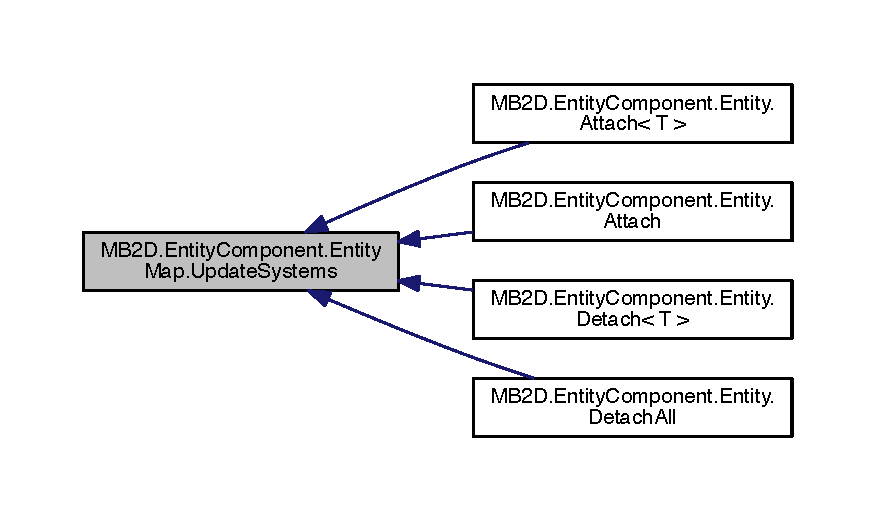
\includegraphics[width=350pt]{class_m_b2_d_1_1_entity_component_1_1_entity_map_ab6078e0b6eddb220b9bbf5d358d6e365_icgraph}
\end{center}
\end{figure}


\subsubsection{Property Documentation}
\hypertarget{class_m_b2_d_1_1_entity_component_1_1_entity_map_a607d25be9724ca759ecef96fe76ee516}{}\label{class_m_b2_d_1_1_entity_component_1_1_entity_map_a607d25be9724ca759ecef96fe76ee516} 
\index{M\+B2\+D\+::\+Entity\+Component\+::\+Entity\+Map@{M\+B2\+D\+::\+Entity\+Component\+::\+Entity\+Map}!Entity\+Count@{Entity\+Count}}
\index{Entity\+Count@{Entity\+Count}!M\+B2\+D\+::\+Entity\+Component\+::\+Entity\+Map@{M\+B2\+D\+::\+Entity\+Component\+::\+Entity\+Map}}
\paragraph{\texorpdfstring{Entity\+Count}{EntityCount}}
{\footnotesize\ttfamily int M\+B2\+D.\+Entity\+Component.\+Entity\+Map.\+Entity\+Count\hspace{0.3cm}{\ttfamily [get]}}



Gets the number of entities in the map. 

The entity count.\hypertarget{class_m_b2_d_1_1_entity_component_1_1_entity_map_a812155313251122f297b6653ab4f4ec1}{}\label{class_m_b2_d_1_1_entity_component_1_1_entity_map_a812155313251122f297b6653ab4f4ec1} 
\index{M\+B2\+D\+::\+Entity\+Component\+::\+Entity\+Map@{M\+B2\+D\+::\+Entity\+Component\+::\+Entity\+Map}!Next\+ID@{Next\+ID}}
\index{Next\+ID@{Next\+ID}!M\+B2\+D\+::\+Entity\+Component\+::\+Entity\+Map@{M\+B2\+D\+::\+Entity\+Component\+::\+Entity\+Map}}
\paragraph{\texorpdfstring{Next\+ID}{NextID}}
{\footnotesize\ttfamily ulong M\+B2\+D.\+Entity\+Component.\+Entity\+Map.\+Next\+ID\hspace{0.3cm}{\ttfamily [get]}}



Auto-\/increments the last generated G\+U\+ID and retrieves the result 

The next identifier.\hypertarget{class_m_b2_d_1_1_entity_component_1_1_entity_map_ae29ad08673cc4c756b43bd3a72c35b84}{}\label{class_m_b2_d_1_1_entity_component_1_1_entity_map_ae29ad08673cc4c756b43bd3a72c35b84} 
\index{M\+B2\+D\+::\+Entity\+Component\+::\+Entity\+Map@{M\+B2\+D\+::\+Entity\+Component\+::\+Entity\+Map}!this\mbox{[}string key\mbox{]}@{this[string key]}}
\index{this\mbox{[}string key\mbox{]}@{this[string key]}!M\+B2\+D\+::\+Entity\+Component\+::\+Entity\+Map@{M\+B2\+D\+::\+Entity\+Component\+::\+Entity\+Map}}
\paragraph{\texorpdfstring{this[string key]}{this[string key]}}
{\footnotesize\ttfamily \hyperlink{class_m_b2_d_1_1_entity_component_1_1_entity}{Entity} M\+B2\+D.\+Entity\+Component.\+Entity\+Map.\+this\mbox{[}string key\mbox{]}\hspace{0.3cm}{\ttfamily [get]}}



Gets the T\+:\+M\+B2\+D.\+Entity\+Component.\+Entity with the specified tag if it exists; null otherwise 


\begin{DoxyParams}{Parameters}
{\em key} & Tagname of the entity to retireve.\\
\hline
\end{DoxyParams}


The documentation for this class was generated from the following file\+:\begin{DoxyCompactItemize}
\item 
M\+B2\+D/src/\+Entity\+Component/Entity\+Map.\+cs\end{DoxyCompactItemize}

\hypertarget{class_m_b2_d_1_1_entity_component_1_1_entity_system}{}\subsection{M\+B2\+D.\+Entity\+Component.\+Entity\+System Class Reference}
\label{class_m_b2_d_1_1_entity_component_1_1_entity_system}\index{M\+B2\+D.\+Entity\+Component.\+Entity\+System@{M\+B2\+D.\+Entity\+Component.\+Entity\+System}}


Performs logic on an entity.  




Inheritance diagram for M\+B2\+D.\+Entity\+Component.\+Entity\+System\+:
\nopagebreak
\begin{figure}[H]
\begin{center}
\leavevmode
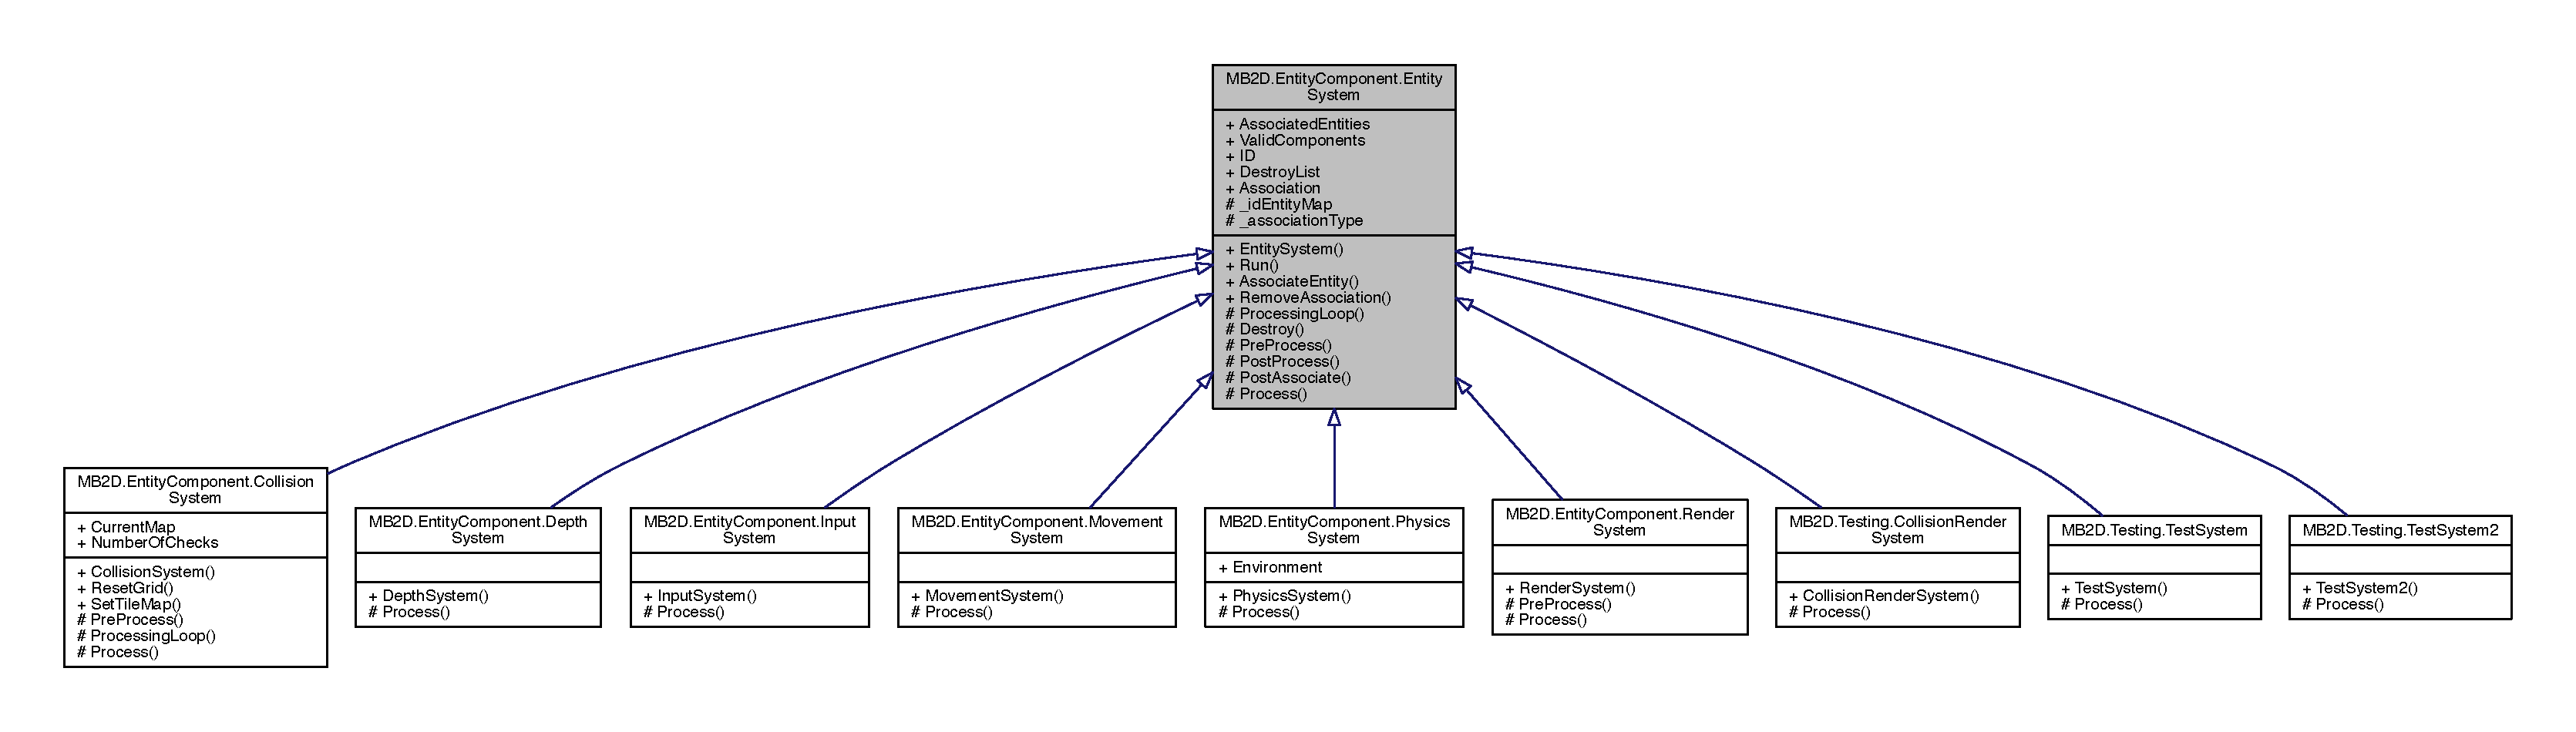
\includegraphics[width=350pt]{class_m_b2_d_1_1_entity_component_1_1_entity_system__inherit__graph}
\end{center}
\end{figure}


Collaboration diagram for M\+B2\+D.\+Entity\+Component.\+Entity\+System\+:
\nopagebreak
\begin{figure}[H]
\begin{center}
\leavevmode
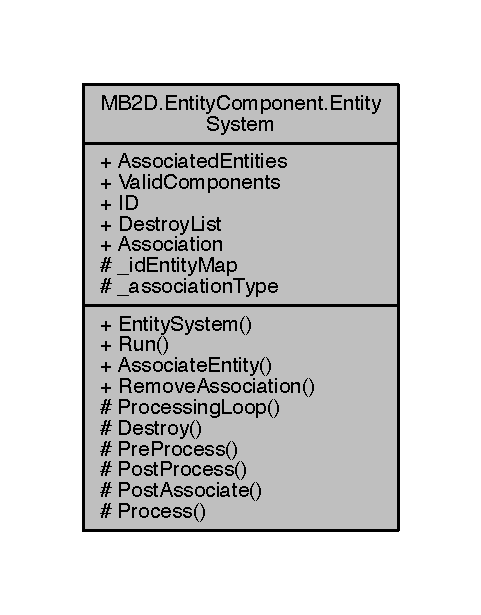
\includegraphics[width=231pt]{class_m_b2_d_1_1_entity_component_1_1_entity_system__coll__graph}
\end{center}
\end{figure}
\subsubsection*{Public Member Functions}
\begin{DoxyCompactItemize}
\item 
\hyperlink{class_m_b2_d_1_1_entity_component_1_1_entity_system_abc7175246313b23db881d09da586428a}{Entity\+System} (params Type\mbox{[}$\,$\mbox{]} components)
\begin{DoxyCompactList}\small\item\em Initializes a new instance of the T\+:\+M\+B2\+D.\+Entity\+Component.\+Entity\+System class. Checks if the passed in types are valid components and if not, all components are deregistered leaving a system that knows about nothing and can\textquotesingle{}t operate on any entities. \end{DoxyCompactList}\item 
void \hyperlink{class_m_b2_d_1_1_entity_component_1_1_entity_system_a3a1a74c4d3f8f0f452e0cdaa5515face}{Run} ()
\begin{DoxyCompactList}\small\item\em Runs this systems \hyperlink{class_m_b2_d_1_1_entity_component_1_1_entity_system_abbf83b87cb5d12754fb058cef50451fa}{Process()} method on all entities \end{DoxyCompactList}\item 
void \hyperlink{class_m_b2_d_1_1_entity_component_1_1_entity_system_aaf18ceb985015ddbff4a361a3b1de5bb}{Associate\+Entity} (\hyperlink{class_m_b2_d_1_1_entity_component_1_1_entity}{Entity} entity)
\begin{DoxyCompactList}\small\item\em Associates a new entity with this system. \end{DoxyCompactList}\item 
void \hyperlink{class_m_b2_d_1_1_entity_component_1_1_entity_system_a6fa9406e1f4a0ca8ddf21cf04be3abe3}{Remove\+Association} (\hyperlink{class_m_b2_d_1_1_entity_component_1_1_entity}{Entity} entity)
\begin{DoxyCompactList}\small\item\em Decouples an association with this system \end{DoxyCompactList}\end{DoxyCompactItemize}
\subsubsection*{Protected Member Functions}
\begin{DoxyCompactItemize}
\item 
virtual void \hyperlink{class_m_b2_d_1_1_entity_component_1_1_entity_system_a75552787342e68c427bf2e1ffa60ed6c}{Processing\+Loop} ()
\begin{DoxyCompactList}\small\item\em Executes \hyperlink{class_m_b2_d_1_1_entity_component_1_1_entity_system_abbf83b87cb5d12754fb058cef50451fa}{Process()} on all Associated\+Entities. \end{DoxyCompactList}\item 
void \hyperlink{class_m_b2_d_1_1_entity_component_1_1_entity_system_a86f27e2e12da562903092d5afb9dd70d}{Destroy} (\hyperlink{class_m_b2_d_1_1_entity_component_1_1_entity}{Entity} entity)
\begin{DoxyCompactList}\small\item\em Adds the specific entity to the destroy list to be cleaned up the next time a system is run \end{DoxyCompactList}\item 
virtual void \hyperlink{class_m_b2_d_1_1_entity_component_1_1_entity_system_aadc002dd04d9cb75775ca955a28e303e}{Pre\+Process} ()
\begin{DoxyCompactList}\small\item\em Used to setup any data needed before processing all entities, such as sorting a list ahead of time \end{DoxyCompactList}\item 
virtual void \hyperlink{class_m_b2_d_1_1_entity_component_1_1_entity_system_aa215c796a01092b66eb70c5726dfac75}{Post\+Process} ()
\begin{DoxyCompactList}\small\item\em Used to cleanup or execute any teardown logic needed \end{DoxyCompactList}\item 
virtual void \hyperlink{class_m_b2_d_1_1_entity_component_1_1_entity_system_ae8d1330e220d3ae7c8f6640c5d4aacd0}{Post\+Associate} (\hyperlink{class_m_b2_d_1_1_entity_component_1_1_entity}{Entity} entity)
\begin{DoxyCompactList}\small\item\em Used to define any logic or extra data needed after an entity is associated with the system. \end{DoxyCompactList}\item 
abstract void \hyperlink{class_m_b2_d_1_1_entity_component_1_1_entity_system_abbf83b87cb5d12754fb058cef50451fa}{Process} (\hyperlink{class_m_b2_d_1_1_entity_component_1_1_entity}{Entity} entity)
\begin{DoxyCompactList}\small\item\em Executes this systems logic on a single entity \end{DoxyCompactList}\end{DoxyCompactItemize}
\subsubsection*{Protected Attributes}
\begin{DoxyCompactItemize}
\item 
Dictionary$<$ ulong, \hyperlink{class_m_b2_d_1_1_entity_component_1_1_entity}{Entity} $>$ \hyperlink{class_m_b2_d_1_1_entity_component_1_1_entity_system_a7415c4bff1132bb4dadcc1a072c663da}{\+\_\+id\+Entity\+Map}
\begin{DoxyCompactList}\small\item\em All G\+U\+ID\textquotesingle{}s of entities this system knows about \end{DoxyCompactList}\item 
Entity\+Association \hyperlink{class_m_b2_d_1_1_entity_component_1_1_entity_system_a1e5512e27d2cf3f40dcf8f39975ca1d7}{\+\_\+association\+Type}
\begin{DoxyCompactList}\small\item\em Defines if this system should be Loose or Strict \end{DoxyCompactList}\end{DoxyCompactItemize}
\subsubsection*{Properties}
\begin{DoxyCompactItemize}
\item 
List$<$ \hyperlink{class_m_b2_d_1_1_entity_component_1_1_entity}{Entity} $>$ \hyperlink{class_m_b2_d_1_1_entity_component_1_1_entity_system_a1c442059af272594b0485832c9f44e94}{Associated\+Entities}\hspace{0.3cm}{\ttfamily  \mbox{[}get, set\mbox{]}}
\begin{DoxyCompactList}\small\item\em Gets or sets the associated entities list. \end{DoxyCompactList}\item 
List$<$ Type $>$ \hyperlink{class_m_b2_d_1_1_entity_component_1_1_entity_system_ad78a75cc9b9bd5a4250ea725dbde3300}{Valid\+Components}\hspace{0.3cm}{\ttfamily  \mbox{[}get\mbox{]}}
\begin{DoxyCompactList}\small\item\em Gets the list of components this system is interested in \end{DoxyCompactList}\item 
ulong \hyperlink{class_m_b2_d_1_1_entity_component_1_1_entity_system_a33c31c8fda2901b2bebd71caf39c0d23}{ID}\hspace{0.3cm}{\ttfamily  \mbox{[}get, set\mbox{]}}
\begin{DoxyCompactList}\small\item\em Gets or sets this systems ID mask \end{DoxyCompactList}\item 
List$<$ \hyperlink{class_m_b2_d_1_1_entity_component_1_1_entity}{Entity} $>$ \hyperlink{class_m_b2_d_1_1_entity_component_1_1_entity_system_a9da3b207e098aa5fcc6ceb2aa3d247d8}{Destroy\+List}\hspace{0.3cm}{\ttfamily  \mbox{[}get\mbox{]}}
\begin{DoxyCompactList}\small\item\em Gets the destroy list. \end{DoxyCompactList}\item 
Entity\+Association \hyperlink{class_m_b2_d_1_1_entity_component_1_1_entity_system_af68858392489a7aab3c91122ab48865f}{Association}\hspace{0.3cm}{\ttfamily  \mbox{[}get\mbox{]}}
\begin{DoxyCompactList}\small\item\em Gets the systems association level. \end{DoxyCompactList}\end{DoxyCompactItemize}


\subsubsection{Detailed Description}
Performs logic on an entity. 



\subsubsection{Constructor \& Destructor Documentation}
\hypertarget{class_m_b2_d_1_1_entity_component_1_1_entity_system_abc7175246313b23db881d09da586428a}{}\label{class_m_b2_d_1_1_entity_component_1_1_entity_system_abc7175246313b23db881d09da586428a} 
\index{M\+B2\+D\+::\+Entity\+Component\+::\+Entity\+System@{M\+B2\+D\+::\+Entity\+Component\+::\+Entity\+System}!Entity\+System@{Entity\+System}}
\index{Entity\+System@{Entity\+System}!M\+B2\+D\+::\+Entity\+Component\+::\+Entity\+System@{M\+B2\+D\+::\+Entity\+Component\+::\+Entity\+System}}
\paragraph{\texorpdfstring{Entity\+System()}{EntitySystem()}}
{\footnotesize\ttfamily M\+B2\+D.\+Entity\+Component.\+Entity\+System.\+Entity\+System (\begin{DoxyParamCaption}\item[{params Type \mbox{[}$\,$\mbox{]}}]{components }\end{DoxyParamCaption})\hspace{0.3cm}{\ttfamily [inline]}}



Initializes a new instance of the T\+:\+M\+B2\+D.\+Entity\+Component.\+Entity\+System class. Checks if the passed in types are valid components and if not, all components are deregistered leaving a system that knows about nothing and can\textquotesingle{}t operate on any entities. 


\begin{DoxyParams}{Parameters}
{\em components} & Components this system is interested in\\
\hline
\end{DoxyParams}


\subsubsection{Member Function Documentation}
\hypertarget{class_m_b2_d_1_1_entity_component_1_1_entity_system_aaf18ceb985015ddbff4a361a3b1de5bb}{}\label{class_m_b2_d_1_1_entity_component_1_1_entity_system_aaf18ceb985015ddbff4a361a3b1de5bb} 
\index{M\+B2\+D\+::\+Entity\+Component\+::\+Entity\+System@{M\+B2\+D\+::\+Entity\+Component\+::\+Entity\+System}!Associate\+Entity@{Associate\+Entity}}
\index{Associate\+Entity@{Associate\+Entity}!M\+B2\+D\+::\+Entity\+Component\+::\+Entity\+System@{M\+B2\+D\+::\+Entity\+Component\+::\+Entity\+System}}
\paragraph{\texorpdfstring{Associate\+Entity()}{AssociateEntity()}}
{\footnotesize\ttfamily void M\+B2\+D.\+Entity\+Component.\+Entity\+System.\+Associate\+Entity (\begin{DoxyParamCaption}\item[{\hyperlink{class_m_b2_d_1_1_entity_component_1_1_entity}{Entity}}]{entity }\end{DoxyParamCaption})\hspace{0.3cm}{\ttfamily [inline]}}



Associates a new entity with this system. 


\begin{DoxyParams}{Parameters}
{\em entity} & \hyperlink{class_m_b2_d_1_1_entity_component_1_1_entity}{Entity} to associate\\
\hline
\end{DoxyParams}
\hypertarget{class_m_b2_d_1_1_entity_component_1_1_entity_system_a86f27e2e12da562903092d5afb9dd70d}{}\label{class_m_b2_d_1_1_entity_component_1_1_entity_system_a86f27e2e12da562903092d5afb9dd70d} 
\index{M\+B2\+D\+::\+Entity\+Component\+::\+Entity\+System@{M\+B2\+D\+::\+Entity\+Component\+::\+Entity\+System}!Destroy@{Destroy}}
\index{Destroy@{Destroy}!M\+B2\+D\+::\+Entity\+Component\+::\+Entity\+System@{M\+B2\+D\+::\+Entity\+Component\+::\+Entity\+System}}
\paragraph{\texorpdfstring{Destroy()}{Destroy()}}
{\footnotesize\ttfamily void M\+B2\+D.\+Entity\+Component.\+Entity\+System.\+Destroy (\begin{DoxyParamCaption}\item[{\hyperlink{class_m_b2_d_1_1_entity_component_1_1_entity}{Entity}}]{entity }\end{DoxyParamCaption})\hspace{0.3cm}{\ttfamily [inline]}, {\ttfamily [protected]}}



Adds the specific entity to the destroy list to be cleaned up the next time a system is run 


\begin{DoxyParams}{Parameters}
{\em entity} & \hyperlink{class_m_b2_d_1_1_entity_component_1_1_entity}{Entity} to destroy.\\
\hline
\end{DoxyParams}
\hypertarget{class_m_b2_d_1_1_entity_component_1_1_entity_system_ae8d1330e220d3ae7c8f6640c5d4aacd0}{}\label{class_m_b2_d_1_1_entity_component_1_1_entity_system_ae8d1330e220d3ae7c8f6640c5d4aacd0} 
\index{M\+B2\+D\+::\+Entity\+Component\+::\+Entity\+System@{M\+B2\+D\+::\+Entity\+Component\+::\+Entity\+System}!Post\+Associate@{Post\+Associate}}
\index{Post\+Associate@{Post\+Associate}!M\+B2\+D\+::\+Entity\+Component\+::\+Entity\+System@{M\+B2\+D\+::\+Entity\+Component\+::\+Entity\+System}}
\paragraph{\texorpdfstring{Post\+Associate()}{PostAssociate()}}
{\footnotesize\ttfamily virtual void M\+B2\+D.\+Entity\+Component.\+Entity\+System.\+Post\+Associate (\begin{DoxyParamCaption}\item[{\hyperlink{class_m_b2_d_1_1_entity_component_1_1_entity}{Entity}}]{entity }\end{DoxyParamCaption})\hspace{0.3cm}{\ttfamily [inline]}, {\ttfamily [protected]}, {\ttfamily [virtual]}}



Used to define any logic or extra data needed after an entity is associated with the system. 


\begin{DoxyParams}{Parameters}
{\em entity} & \hyperlink{class_m_b2_d_1_1_entity_component_1_1_entity}{Entity}.\\
\hline
\end{DoxyParams}
\hypertarget{class_m_b2_d_1_1_entity_component_1_1_entity_system_aa215c796a01092b66eb70c5726dfac75}{}\label{class_m_b2_d_1_1_entity_component_1_1_entity_system_aa215c796a01092b66eb70c5726dfac75} 
\index{M\+B2\+D\+::\+Entity\+Component\+::\+Entity\+System@{M\+B2\+D\+::\+Entity\+Component\+::\+Entity\+System}!Post\+Process@{Post\+Process}}
\index{Post\+Process@{Post\+Process}!M\+B2\+D\+::\+Entity\+Component\+::\+Entity\+System@{M\+B2\+D\+::\+Entity\+Component\+::\+Entity\+System}}
\paragraph{\texorpdfstring{Post\+Process()}{PostProcess()}}
{\footnotesize\ttfamily virtual void M\+B2\+D.\+Entity\+Component.\+Entity\+System.\+Post\+Process (\begin{DoxyParamCaption}{ }\end{DoxyParamCaption})\hspace{0.3cm}{\ttfamily [inline]}, {\ttfamily [protected]}, {\ttfamily [virtual]}}



Used to cleanup or execute any teardown logic needed 

\hypertarget{class_m_b2_d_1_1_entity_component_1_1_entity_system_aadc002dd04d9cb75775ca955a28e303e}{}\label{class_m_b2_d_1_1_entity_component_1_1_entity_system_aadc002dd04d9cb75775ca955a28e303e} 
\index{M\+B2\+D\+::\+Entity\+Component\+::\+Entity\+System@{M\+B2\+D\+::\+Entity\+Component\+::\+Entity\+System}!Pre\+Process@{Pre\+Process}}
\index{Pre\+Process@{Pre\+Process}!M\+B2\+D\+::\+Entity\+Component\+::\+Entity\+System@{M\+B2\+D\+::\+Entity\+Component\+::\+Entity\+System}}
\paragraph{\texorpdfstring{Pre\+Process()}{PreProcess()}}
{\footnotesize\ttfamily virtual void M\+B2\+D.\+Entity\+Component.\+Entity\+System.\+Pre\+Process (\begin{DoxyParamCaption}{ }\end{DoxyParamCaption})\hspace{0.3cm}{\ttfamily [inline]}, {\ttfamily [protected]}, {\ttfamily [virtual]}}



Used to setup any data needed before processing all entities, such as sorting a list ahead of time 



Reimplemented in \hyperlink{class_m_b2_d_1_1_entity_component_1_1_collision_system_ad591227767c8b6c66ca3891de04e9050}{M\+B2\+D.\+Entity\+Component.\+Collision\+System}, and \hyperlink{class_m_b2_d_1_1_entity_component_1_1_render_system_aadd36efe73a5f8cc489894232a5fc201}{M\+B2\+D.\+Entity\+Component.\+Render\+System}.

\hypertarget{class_m_b2_d_1_1_entity_component_1_1_entity_system_abbf83b87cb5d12754fb058cef50451fa}{}\label{class_m_b2_d_1_1_entity_component_1_1_entity_system_abbf83b87cb5d12754fb058cef50451fa} 
\index{M\+B2\+D\+::\+Entity\+Component\+::\+Entity\+System@{M\+B2\+D\+::\+Entity\+Component\+::\+Entity\+System}!Process@{Process}}
\index{Process@{Process}!M\+B2\+D\+::\+Entity\+Component\+::\+Entity\+System@{M\+B2\+D\+::\+Entity\+Component\+::\+Entity\+System}}
\paragraph{\texorpdfstring{Process()}{Process()}}
{\footnotesize\ttfamily abstract void M\+B2\+D.\+Entity\+Component.\+Entity\+System.\+Process (\begin{DoxyParamCaption}\item[{\hyperlink{class_m_b2_d_1_1_entity_component_1_1_entity}{Entity}}]{entity }\end{DoxyParamCaption})\hspace{0.3cm}{\ttfamily [protected]}, {\ttfamily [pure virtual]}}



Executes this systems logic on a single entity 


\begin{DoxyParams}{Parameters}
{\em entity} & \hyperlink{class_m_b2_d_1_1_entity_component_1_1_entity}{Entity} to operate on\\
\hline
\end{DoxyParams}


Implemented in \hyperlink{class_m_b2_d_1_1_entity_component_1_1_collision_system_adfbee070ed7b120565a5f8a08c159535}{M\+B2\+D.\+Entity\+Component.\+Collision\+System}, \hyperlink{class_m_b2_d_1_1_entity_component_1_1_render_system_a015ba5b16cc227c7a5a16fcc1ffa73b7}{M\+B2\+D.\+Entity\+Component.\+Render\+System}, \hyperlink{class_m_b2_d_1_1_testing_1_1_test_system2_a0fbdd06fd0de796cfec32b7e025f73fe}{M\+B2\+D.\+Testing.\+Test\+System2}, \hyperlink{class_m_b2_d_1_1_entity_component_1_1_physics_system_ab8398d3b16f49e684f55649877f645c0}{M\+B2\+D.\+Entity\+Component.\+Physics\+System}, \hyperlink{class_m_b2_d_1_1_testing_1_1_test_system_a35d160e6e7e8ffb8f1a6cf403b00ef40}{M\+B2\+D.\+Testing.\+Test\+System}, \hyperlink{class_m_b2_d_1_1_entity_component_1_1_input_system_afa241f5c32788fc65587e0443f7217b3}{M\+B2\+D.\+Entity\+Component.\+Input\+System}, \hyperlink{class_m_b2_d_1_1_entity_component_1_1_movement_system_afa730fd9080848ce877206c00a744cdf}{M\+B2\+D.\+Entity\+Component.\+Movement\+System}, \hyperlink{class_m_b2_d_1_1_entity_component_1_1_depth_system_a738556bdf819c9c0d4082a323a502c58}{M\+B2\+D.\+Entity\+Component.\+Depth\+System}, and \hyperlink{class_m_b2_d_1_1_testing_1_1_collision_render_system_af7b7ffdb316533a084e98cbea97a096f}{M\+B2\+D.\+Testing.\+Collision\+Render\+System}.

\hypertarget{class_m_b2_d_1_1_entity_component_1_1_entity_system_a75552787342e68c427bf2e1ffa60ed6c}{}\label{class_m_b2_d_1_1_entity_component_1_1_entity_system_a75552787342e68c427bf2e1ffa60ed6c} 
\index{M\+B2\+D\+::\+Entity\+Component\+::\+Entity\+System@{M\+B2\+D\+::\+Entity\+Component\+::\+Entity\+System}!Processing\+Loop@{Processing\+Loop}}
\index{Processing\+Loop@{Processing\+Loop}!M\+B2\+D\+::\+Entity\+Component\+::\+Entity\+System@{M\+B2\+D\+::\+Entity\+Component\+::\+Entity\+System}}
\paragraph{\texorpdfstring{Processing\+Loop()}{ProcessingLoop()}}
{\footnotesize\ttfamily virtual void M\+B2\+D.\+Entity\+Component.\+Entity\+System.\+Processing\+Loop (\begin{DoxyParamCaption}{ }\end{DoxyParamCaption})\hspace{0.3cm}{\ttfamily [inline]}, {\ttfamily [protected]}, {\ttfamily [virtual]}}



Executes \hyperlink{class_m_b2_d_1_1_entity_component_1_1_entity_system_abbf83b87cb5d12754fb058cef50451fa}{Process()} on all Associated\+Entities. 



Reimplemented in \hyperlink{class_m_b2_d_1_1_entity_component_1_1_collision_system_a06249adc606475cdc35f28783a1b27c4}{M\+B2\+D.\+Entity\+Component.\+Collision\+System}.

\hypertarget{class_m_b2_d_1_1_entity_component_1_1_entity_system_a6fa9406e1f4a0ca8ddf21cf04be3abe3}{}\label{class_m_b2_d_1_1_entity_component_1_1_entity_system_a6fa9406e1f4a0ca8ddf21cf04be3abe3} 
\index{M\+B2\+D\+::\+Entity\+Component\+::\+Entity\+System@{M\+B2\+D\+::\+Entity\+Component\+::\+Entity\+System}!Remove\+Association@{Remove\+Association}}
\index{Remove\+Association@{Remove\+Association}!M\+B2\+D\+::\+Entity\+Component\+::\+Entity\+System@{M\+B2\+D\+::\+Entity\+Component\+::\+Entity\+System}}
\paragraph{\texorpdfstring{Remove\+Association()}{RemoveAssociation()}}
{\footnotesize\ttfamily void M\+B2\+D.\+Entity\+Component.\+Entity\+System.\+Remove\+Association (\begin{DoxyParamCaption}\item[{\hyperlink{class_m_b2_d_1_1_entity_component_1_1_entity}{Entity}}]{entity }\end{DoxyParamCaption})\hspace{0.3cm}{\ttfamily [inline]}}



Decouples an association with this system 


\begin{DoxyParams}{Parameters}
{\em entity} & \hyperlink{class_m_b2_d_1_1_entity_component_1_1_entity}{Entity} to decouple.\\
\hline
\end{DoxyParams}
\hypertarget{class_m_b2_d_1_1_entity_component_1_1_entity_system_a3a1a74c4d3f8f0f452e0cdaa5515face}{}\label{class_m_b2_d_1_1_entity_component_1_1_entity_system_a3a1a74c4d3f8f0f452e0cdaa5515face} 
\index{M\+B2\+D\+::\+Entity\+Component\+::\+Entity\+System@{M\+B2\+D\+::\+Entity\+Component\+::\+Entity\+System}!Run@{Run}}
\index{Run@{Run}!M\+B2\+D\+::\+Entity\+Component\+::\+Entity\+System@{M\+B2\+D\+::\+Entity\+Component\+::\+Entity\+System}}
\paragraph{\texorpdfstring{Run()}{Run()}}
{\footnotesize\ttfamily void M\+B2\+D.\+Entity\+Component.\+Entity\+System.\+Run (\begin{DoxyParamCaption}{ }\end{DoxyParamCaption})\hspace{0.3cm}{\ttfamily [inline]}}



Runs this systems \hyperlink{class_m_b2_d_1_1_entity_component_1_1_entity_system_abbf83b87cb5d12754fb058cef50451fa}{Process()} method on all entities 



\subsubsection{Member Data Documentation}
\hypertarget{class_m_b2_d_1_1_entity_component_1_1_entity_system_a1e5512e27d2cf3f40dcf8f39975ca1d7}{}\label{class_m_b2_d_1_1_entity_component_1_1_entity_system_a1e5512e27d2cf3f40dcf8f39975ca1d7} 
\index{M\+B2\+D\+::\+Entity\+Component\+::\+Entity\+System@{M\+B2\+D\+::\+Entity\+Component\+::\+Entity\+System}!\+\_\+association\+Type@{\+\_\+association\+Type}}
\index{\+\_\+association\+Type@{\+\_\+association\+Type}!M\+B2\+D\+::\+Entity\+Component\+::\+Entity\+System@{M\+B2\+D\+::\+Entity\+Component\+::\+Entity\+System}}
\paragraph{\texorpdfstring{\+\_\+association\+Type}{\_associationType}}
{\footnotesize\ttfamily Entity\+Association M\+B2\+D.\+Entity\+Component.\+Entity\+System.\+\_\+association\+Type\hspace{0.3cm}{\ttfamily [protected]}}



Defines if this system should be Loose or Strict 

\hypertarget{class_m_b2_d_1_1_entity_component_1_1_entity_system_a7415c4bff1132bb4dadcc1a072c663da}{}\label{class_m_b2_d_1_1_entity_component_1_1_entity_system_a7415c4bff1132bb4dadcc1a072c663da} 
\index{M\+B2\+D\+::\+Entity\+Component\+::\+Entity\+System@{M\+B2\+D\+::\+Entity\+Component\+::\+Entity\+System}!\+\_\+id\+Entity\+Map@{\+\_\+id\+Entity\+Map}}
\index{\+\_\+id\+Entity\+Map@{\+\_\+id\+Entity\+Map}!M\+B2\+D\+::\+Entity\+Component\+::\+Entity\+System@{M\+B2\+D\+::\+Entity\+Component\+::\+Entity\+System}}
\paragraph{\texorpdfstring{\+\_\+id\+Entity\+Map}{\_idEntityMap}}
{\footnotesize\ttfamily Dictionary$<$ulong, \hyperlink{class_m_b2_d_1_1_entity_component_1_1_entity}{Entity}$>$ M\+B2\+D.\+Entity\+Component.\+Entity\+System.\+\_\+id\+Entity\+Map\hspace{0.3cm}{\ttfamily [protected]}}



All G\+U\+ID\textquotesingle{}s of entities this system knows about 



\subsubsection{Property Documentation}
\hypertarget{class_m_b2_d_1_1_entity_component_1_1_entity_system_a1c442059af272594b0485832c9f44e94}{}\label{class_m_b2_d_1_1_entity_component_1_1_entity_system_a1c442059af272594b0485832c9f44e94} 
\index{M\+B2\+D\+::\+Entity\+Component\+::\+Entity\+System@{M\+B2\+D\+::\+Entity\+Component\+::\+Entity\+System}!Associated\+Entities@{Associated\+Entities}}
\index{Associated\+Entities@{Associated\+Entities}!M\+B2\+D\+::\+Entity\+Component\+::\+Entity\+System@{M\+B2\+D\+::\+Entity\+Component\+::\+Entity\+System}}
\paragraph{\texorpdfstring{Associated\+Entities}{AssociatedEntities}}
{\footnotesize\ttfamily List$<$\hyperlink{class_m_b2_d_1_1_entity_component_1_1_entity}{Entity}$>$ M\+B2\+D.\+Entity\+Component.\+Entity\+System.\+Associated\+Entities\hspace{0.3cm}{\ttfamily [get]}, {\ttfamily [set]}}



Gets or sets the associated entities list. 

The associated entities.\hypertarget{class_m_b2_d_1_1_entity_component_1_1_entity_system_af68858392489a7aab3c91122ab48865f}{}\label{class_m_b2_d_1_1_entity_component_1_1_entity_system_af68858392489a7aab3c91122ab48865f} 
\index{M\+B2\+D\+::\+Entity\+Component\+::\+Entity\+System@{M\+B2\+D\+::\+Entity\+Component\+::\+Entity\+System}!Association@{Association}}
\index{Association@{Association}!M\+B2\+D\+::\+Entity\+Component\+::\+Entity\+System@{M\+B2\+D\+::\+Entity\+Component\+::\+Entity\+System}}
\paragraph{\texorpdfstring{Association}{Association}}
{\footnotesize\ttfamily Entity\+Association M\+B2\+D.\+Entity\+Component.\+Entity\+System.\+Association\hspace{0.3cm}{\ttfamily [get]}}



Gets the systems association level. 

The association level.\hypertarget{class_m_b2_d_1_1_entity_component_1_1_entity_system_a9da3b207e098aa5fcc6ceb2aa3d247d8}{}\label{class_m_b2_d_1_1_entity_component_1_1_entity_system_a9da3b207e098aa5fcc6ceb2aa3d247d8} 
\index{M\+B2\+D\+::\+Entity\+Component\+::\+Entity\+System@{M\+B2\+D\+::\+Entity\+Component\+::\+Entity\+System}!Destroy\+List@{Destroy\+List}}
\index{Destroy\+List@{Destroy\+List}!M\+B2\+D\+::\+Entity\+Component\+::\+Entity\+System@{M\+B2\+D\+::\+Entity\+Component\+::\+Entity\+System}}
\paragraph{\texorpdfstring{Destroy\+List}{DestroyList}}
{\footnotesize\ttfamily List$<$\hyperlink{class_m_b2_d_1_1_entity_component_1_1_entity}{Entity}$>$ M\+B2\+D.\+Entity\+Component.\+Entity\+System.\+Destroy\+List\hspace{0.3cm}{\ttfamily [get]}}



Gets the destroy list. 

The destroy list.\hypertarget{class_m_b2_d_1_1_entity_component_1_1_entity_system_a33c31c8fda2901b2bebd71caf39c0d23}{}\label{class_m_b2_d_1_1_entity_component_1_1_entity_system_a33c31c8fda2901b2bebd71caf39c0d23} 
\index{M\+B2\+D\+::\+Entity\+Component\+::\+Entity\+System@{M\+B2\+D\+::\+Entity\+Component\+::\+Entity\+System}!ID@{ID}}
\index{ID@{ID}!M\+B2\+D\+::\+Entity\+Component\+::\+Entity\+System@{M\+B2\+D\+::\+Entity\+Component\+::\+Entity\+System}}
\paragraph{\texorpdfstring{ID}{ID}}
{\footnotesize\ttfamily ulong M\+B2\+D.\+Entity\+Component.\+Entity\+System.\+ID\hspace{0.3cm}{\ttfamily [get]}, {\ttfamily [set]}}



Gets or sets this systems ID mask 

The identifier mask.\hypertarget{class_m_b2_d_1_1_entity_component_1_1_entity_system_ad78a75cc9b9bd5a4250ea725dbde3300}{}\label{class_m_b2_d_1_1_entity_component_1_1_entity_system_ad78a75cc9b9bd5a4250ea725dbde3300} 
\index{M\+B2\+D\+::\+Entity\+Component\+::\+Entity\+System@{M\+B2\+D\+::\+Entity\+Component\+::\+Entity\+System}!Valid\+Components@{Valid\+Components}}
\index{Valid\+Components@{Valid\+Components}!M\+B2\+D\+::\+Entity\+Component\+::\+Entity\+System@{M\+B2\+D\+::\+Entity\+Component\+::\+Entity\+System}}
\paragraph{\texorpdfstring{Valid\+Components}{ValidComponents}}
{\footnotesize\ttfamily List$<$Type$>$ M\+B2\+D.\+Entity\+Component.\+Entity\+System.\+Valid\+Components\hspace{0.3cm}{\ttfamily [get]}}



Gets the list of components this system is interested in 

The valid components.

The documentation for this class was generated from the following file\+:\begin{DoxyCompactItemize}
\item 
M\+B2\+D/src/\+Entity\+Component/Entity\+System.\+cs\end{DoxyCompactItemize}

\hypertarget{class_m_b2_d_1_1_geometry_1_1_grid}{}\section{M\+B2\+D.\+Geometry.\+Grid Class Reference}
\label{class_m_b2_d_1_1_geometry_1_1_grid}\index{M\+B2\+D.\+Geometry.\+Grid@{M\+B2\+D.\+Geometry.\+Grid}}


Represents a grid structure. Can be drawn via a Sprite\+Batch  




Collaboration diagram for M\+B2\+D.\+Geometry.\+Grid\+:\nopagebreak
\begin{figure}[H]
\begin{center}
\leavevmode
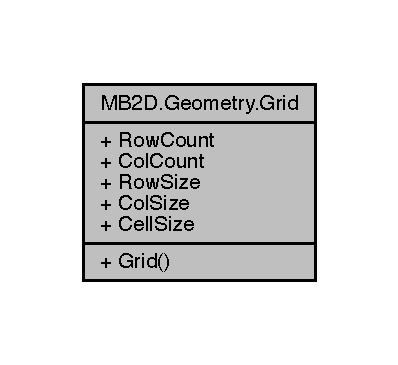
\includegraphics[width=191pt]{class_m_b2_d_1_1_geometry_1_1_grid__coll__graph}
\end{center}
\end{figure}
\subsection*{Public Member Functions}
\begin{DoxyCompactItemize}
\item 
\hyperlink{class_m_b2_d_1_1_geometry_1_1_grid_a7ff870c0156e2fb0fc5fffe081db4a10}{Grid} (int rows, int cols, int row\+Size, int col\+Size)
\begin{DoxyCompactList}\small\item\em Initializes a new instance of the T\+:\+M\+B2\+D.\+Geometry.\+Grid class. \end{DoxyCompactList}\end{DoxyCompactItemize}
\subsection*{Properties}
\begin{DoxyCompactItemize}
\item 
int \hyperlink{class_m_b2_d_1_1_geometry_1_1_grid_ad2599c5d630bb783ff2ba062c276be9a}{Row\+Count}\hspace{0.3cm}{\ttfamily  \mbox{[}get, set\mbox{]}}
\begin{DoxyCompactList}\small\item\em Gets or sets the number of rows. \end{DoxyCompactList}\item 
int \hyperlink{class_m_b2_d_1_1_geometry_1_1_grid_a515c09f56ad55f3742b6a0eccdb15856}{Col\+Count}\hspace{0.3cm}{\ttfamily  \mbox{[}get, set\mbox{]}}
\begin{DoxyCompactList}\small\item\em Gets or sets the number of columns. \end{DoxyCompactList}\item 
int \hyperlink{class_m_b2_d_1_1_geometry_1_1_grid_a38536c42bc3d3d5e58d648fd7b7f8e17}{Row\+Size}\hspace{0.3cm}{\ttfamily  \mbox{[}get, set\mbox{]}}
\begin{DoxyCompactList}\small\item\em Gets or sets the size of each row. \end{DoxyCompactList}\item 
int \hyperlink{class_m_b2_d_1_1_geometry_1_1_grid_aef6e8277c73fcb160fa551836f3685da}{Col\+Size}\hspace{0.3cm}{\ttfamily  \mbox{[}get, set\mbox{]}}
\begin{DoxyCompactList}\small\item\em Gets or sets the size of each column. \end{DoxyCompactList}\item 
Vector2 \hyperlink{class_m_b2_d_1_1_geometry_1_1_grid_afdee3fa9df7802b3b15aa8785621a110}{Cell\+Size}\hspace{0.3cm}{\ttfamily  \mbox{[}get\mbox{]}}
\begin{DoxyCompactList}\small\item\em Gets the size of each cell. \end{DoxyCompactList}\end{DoxyCompactItemize}


\subsection{Detailed Description}
Represents a grid structure. Can be drawn via a Sprite\+Batch 



\subsection{Constructor \& Destructor Documentation}
\hypertarget{class_m_b2_d_1_1_geometry_1_1_grid_a7ff870c0156e2fb0fc5fffe081db4a10}{}\label{class_m_b2_d_1_1_geometry_1_1_grid_a7ff870c0156e2fb0fc5fffe081db4a10} 
\index{M\+B2\+D\+::\+Geometry\+::\+Grid@{M\+B2\+D\+::\+Geometry\+::\+Grid}!Grid@{Grid}}
\index{Grid@{Grid}!M\+B2\+D\+::\+Geometry\+::\+Grid@{M\+B2\+D\+::\+Geometry\+::\+Grid}}
\subsubsection{\texorpdfstring{Grid()}{Grid()}}
{\footnotesize\ttfamily M\+B2\+D.\+Geometry.\+Grid.\+Grid (\begin{DoxyParamCaption}\item[{int}]{rows,  }\item[{int}]{cols,  }\item[{int}]{row\+Size,  }\item[{int}]{col\+Size }\end{DoxyParamCaption})\hspace{0.3cm}{\ttfamily [inline]}}



Initializes a new instance of the T\+:\+M\+B2\+D.\+Geometry.\+Grid class. 


\begin{DoxyParams}{Parameters}
{\em rows} & Number of rows\\
\hline
{\em cols} & Number of columns\\
\hline
{\em row\+Size} & Size of each row\\
\hline
{\em col\+Size} & Size of each column\\
\hline
\end{DoxyParams}


\subsection{Property Documentation}
\hypertarget{class_m_b2_d_1_1_geometry_1_1_grid_afdee3fa9df7802b3b15aa8785621a110}{}\label{class_m_b2_d_1_1_geometry_1_1_grid_afdee3fa9df7802b3b15aa8785621a110} 
\index{M\+B2\+D\+::\+Geometry\+::\+Grid@{M\+B2\+D\+::\+Geometry\+::\+Grid}!Cell\+Size@{Cell\+Size}}
\index{Cell\+Size@{Cell\+Size}!M\+B2\+D\+::\+Geometry\+::\+Grid@{M\+B2\+D\+::\+Geometry\+::\+Grid}}
\subsubsection{\texorpdfstring{Cell\+Size}{CellSize}}
{\footnotesize\ttfamily Vector2 M\+B2\+D.\+Geometry.\+Grid.\+Cell\+Size\hspace{0.3cm}{\ttfamily [get]}}



Gets the size of each cell. 

The size of each cell.\hypertarget{class_m_b2_d_1_1_geometry_1_1_grid_a515c09f56ad55f3742b6a0eccdb15856}{}\label{class_m_b2_d_1_1_geometry_1_1_grid_a515c09f56ad55f3742b6a0eccdb15856} 
\index{M\+B2\+D\+::\+Geometry\+::\+Grid@{M\+B2\+D\+::\+Geometry\+::\+Grid}!Col\+Count@{Col\+Count}}
\index{Col\+Count@{Col\+Count}!M\+B2\+D\+::\+Geometry\+::\+Grid@{M\+B2\+D\+::\+Geometry\+::\+Grid}}
\subsubsection{\texorpdfstring{Col\+Count}{ColCount}}
{\footnotesize\ttfamily int M\+B2\+D.\+Geometry.\+Grid.\+Col\+Count\hspace{0.3cm}{\ttfamily [get]}, {\ttfamily [set]}}



Gets or sets the number of columns. 

The colomn count.\hypertarget{class_m_b2_d_1_1_geometry_1_1_grid_aef6e8277c73fcb160fa551836f3685da}{}\label{class_m_b2_d_1_1_geometry_1_1_grid_aef6e8277c73fcb160fa551836f3685da} 
\index{M\+B2\+D\+::\+Geometry\+::\+Grid@{M\+B2\+D\+::\+Geometry\+::\+Grid}!Col\+Size@{Col\+Size}}
\index{Col\+Size@{Col\+Size}!M\+B2\+D\+::\+Geometry\+::\+Grid@{M\+B2\+D\+::\+Geometry\+::\+Grid}}
\subsubsection{\texorpdfstring{Col\+Size}{ColSize}}
{\footnotesize\ttfamily int M\+B2\+D.\+Geometry.\+Grid.\+Col\+Size\hspace{0.3cm}{\ttfamily [get]}, {\ttfamily [set]}}



Gets or sets the size of each column. 

The size of each column.\hypertarget{class_m_b2_d_1_1_geometry_1_1_grid_ad2599c5d630bb783ff2ba062c276be9a}{}\label{class_m_b2_d_1_1_geometry_1_1_grid_ad2599c5d630bb783ff2ba062c276be9a} 
\index{M\+B2\+D\+::\+Geometry\+::\+Grid@{M\+B2\+D\+::\+Geometry\+::\+Grid}!Row\+Count@{Row\+Count}}
\index{Row\+Count@{Row\+Count}!M\+B2\+D\+::\+Geometry\+::\+Grid@{M\+B2\+D\+::\+Geometry\+::\+Grid}}
\subsubsection{\texorpdfstring{Row\+Count}{RowCount}}
{\footnotesize\ttfamily int M\+B2\+D.\+Geometry.\+Grid.\+Row\+Count\hspace{0.3cm}{\ttfamily [get]}, {\ttfamily [set]}}



Gets or sets the number of rows. 

The row count.\hypertarget{class_m_b2_d_1_1_geometry_1_1_grid_a38536c42bc3d3d5e58d648fd7b7f8e17}{}\label{class_m_b2_d_1_1_geometry_1_1_grid_a38536c42bc3d3d5e58d648fd7b7f8e17} 
\index{M\+B2\+D\+::\+Geometry\+::\+Grid@{M\+B2\+D\+::\+Geometry\+::\+Grid}!Row\+Size@{Row\+Size}}
\index{Row\+Size@{Row\+Size}!M\+B2\+D\+::\+Geometry\+::\+Grid@{M\+B2\+D\+::\+Geometry\+::\+Grid}}
\subsubsection{\texorpdfstring{Row\+Size}{RowSize}}
{\footnotesize\ttfamily int M\+B2\+D.\+Geometry.\+Grid.\+Row\+Size\hspace{0.3cm}{\ttfamily [get]}, {\ttfamily [set]}}



Gets or sets the size of each row. 

The size of each row.

The documentation for this class was generated from the following file\+:\begin{DoxyCompactItemize}
\item 
M\+B2\+D/src/\+Geometry/Grid.\+cs\end{DoxyCompactItemize}

\hypertarget{interface_m_b2_d_1_1_entity_component_1_1_i_component}{}\section{M\+B2\+D.\+Entity\+Component.\+I\+Component Interface Reference}
\label{interface_m_b2_d_1_1_entity_component_1_1_i_component}\index{M\+B2\+D.\+Entity\+Component.\+I\+Component@{M\+B2\+D.\+Entity\+Component.\+I\+Component}}


Tags any class as a valid component for use in the \hyperlink{class_m_b2_d_1_1_entity_component_1_1_entity_map}{Entity\+Map}. Derived classes should contain no logic, only data fields.  




Inheritance diagram for M\+B2\+D.\+Entity\+Component.\+I\+Component\+:
\nopagebreak
\begin{figure}[H]
\begin{center}
\leavevmode
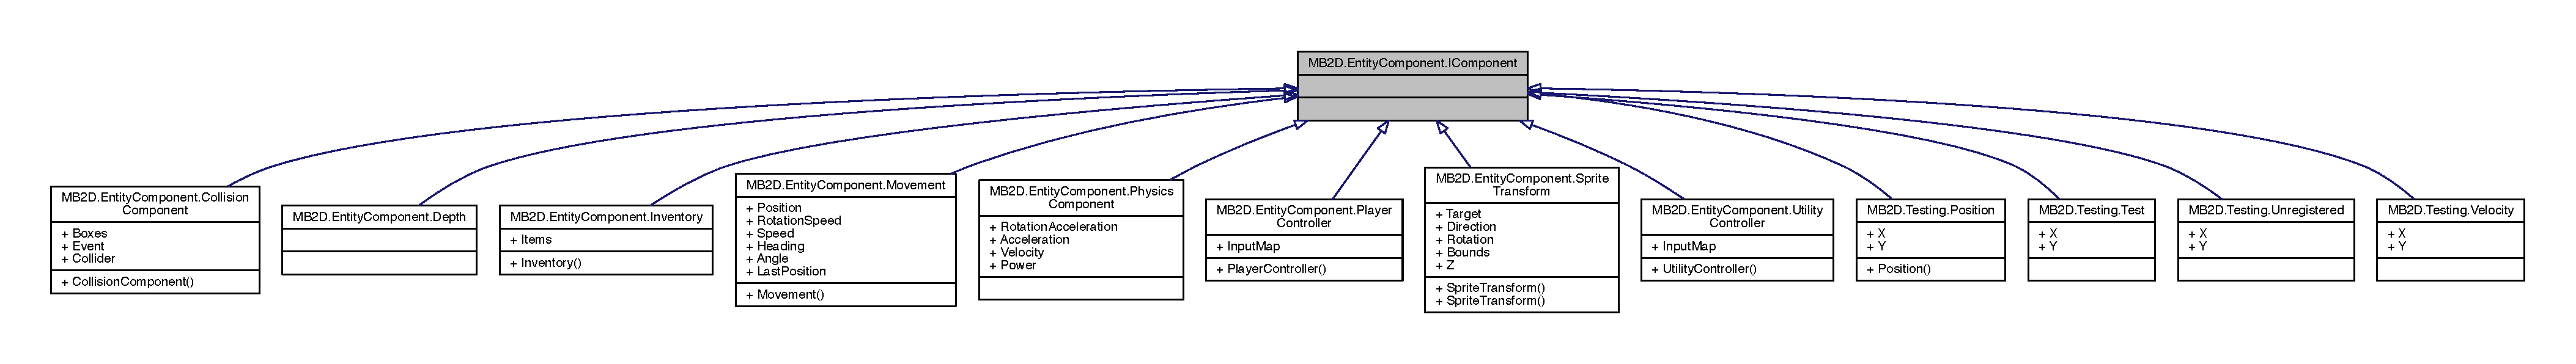
\includegraphics[width=350pt]{interface_m_b2_d_1_1_entity_component_1_1_i_component__inherit__graph}
\end{center}
\end{figure}


Collaboration diagram for M\+B2\+D.\+Entity\+Component.\+I\+Component\+:
\nopagebreak
\begin{figure}[H]
\begin{center}
\leavevmode
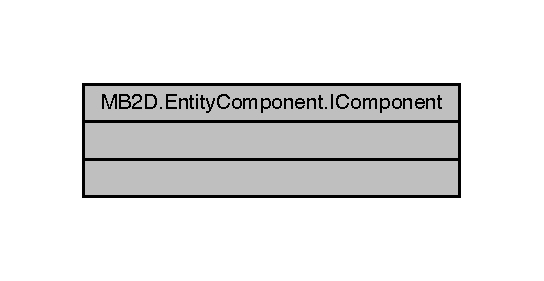
\includegraphics[width=261pt]{interface_m_b2_d_1_1_entity_component_1_1_i_component__coll__graph}
\end{center}
\end{figure}


\subsection{Detailed Description}
Tags any class as a valid component for use in the \hyperlink{class_m_b2_d_1_1_entity_component_1_1_entity_map}{Entity\+Map}. Derived classes should contain no logic, only data fields. 



The documentation for this interface was generated from the following file\+:\begin{DoxyCompactItemize}
\item 
M\+B2\+D/src/\+Entity\+Component/I\+Component.\+cs\end{DoxyCompactItemize}

\hypertarget{class_m_b2_d_1_1_i_o_1_1_input_map}{}\section{M\+B2\+D.\+I\+O.\+Input\+Map Class Reference}
\label{class_m_b2_d_1_1_i_o_1_1_input_map}\index{M\+B2\+D.\+I\+O.\+Input\+Map@{M\+B2\+D.\+I\+O.\+Input\+Map}}


Maps commands to keys and trigger types  




Collaboration diagram for M\+B2\+D.\+I\+O.\+Input\+Map\+:\nopagebreak
\begin{figure}[H]
\begin{center}
\leavevmode
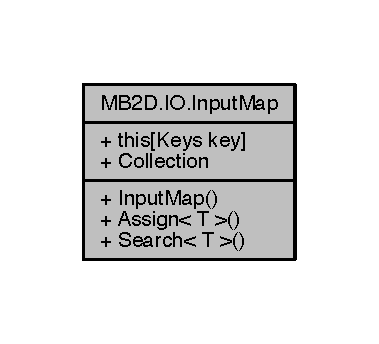
\includegraphics[width=182pt]{class_m_b2_d_1_1_i_o_1_1_input_map__coll__graph}
\end{center}
\end{figure}
\subsection*{Public Member Functions}
\begin{DoxyCompactItemize}
\item 
\hyperlink{class_m_b2_d_1_1_i_o_1_1_input_map_a37cd0d946d9a15c9a5ce96d5ca2ca8f1}{Input\+Map} ()
\begin{DoxyCompactList}\small\item\em Initializes a new instance of the T\+:\+M\+B2\+D.\+I\+O.\+Input\+Map class. \end{DoxyCompactList}\item 
\hyperlink{class_m_b2_d_1_1_i_o_1_1_command}{Command} \hyperlink{class_m_b2_d_1_1_i_o_1_1_input_map_a07131c13b291c957512c08aa0d814890}{Assign$<$ T $>$} (Keys key, \hyperlink{namespace_m_b2_d_1_1_i_o_ab5f95f3fe9e652778b62bdf943168a68}{Command\+Type} type, params object\mbox{[}$\,$\mbox{]} args)
\begin{DoxyCompactList}\small\item\em Assign a \hyperlink{class_m_b2_d_1_1_i_o_1_1_command}{Command} to the specified key and Command\+Type . \end{DoxyCompactList}\item 
T \hyperlink{class_m_b2_d_1_1_i_o_1_1_input_map_ae5537db7c751ba05196cc71d5f98bf87}{Search$<$ T $>$} ()
\begin{DoxyCompactList}\small\item\em Searches the map for a specific command \end{DoxyCompactList}\end{DoxyCompactItemize}
\subsection*{Properties}
\begin{DoxyCompactItemize}
\item 
List$<$ \hyperlink{class_m_b2_d_1_1_i_o_1_1_command}{Command} $>$ \hyperlink{class_m_b2_d_1_1_i_o_1_1_input_map_ad78e010b598d32be8fbd1b30c41b7ee0}{this\mbox{[}\+Keys key\mbox{]}}\hspace{0.3cm}{\ttfamily  \mbox{[}get\mbox{]}}
\begin{DoxyCompactList}\small\item\em Gets the T\+:\+M\+B2\+D.\+I\+O.\+Commnad mapped to the specified key. \end{DoxyCompactList}\item 
Dictionary$<$ Keys, List$<$ \hyperlink{class_m_b2_d_1_1_i_o_1_1_command}{Command} $>$ $>$ \hyperlink{class_m_b2_d_1_1_i_o_1_1_input_map_a16a798fd9e5c599591620b52c5eb8a55}{Collection}\hspace{0.3cm}{\ttfamily  \mbox{[}get\mbox{]}}
\begin{DoxyCompactList}\small\item\em Gets a key-\/$>$\hyperlink{class_m_b2_d_1_1_i_o_1_1_command}{Command} dictionary \end{DoxyCompactList}\end{DoxyCompactItemize}


\subsection{Detailed Description}
Maps commands to keys and trigger types 



\subsection{Constructor \& Destructor Documentation}
\hypertarget{class_m_b2_d_1_1_i_o_1_1_input_map_a37cd0d946d9a15c9a5ce96d5ca2ca8f1}{}\label{class_m_b2_d_1_1_i_o_1_1_input_map_a37cd0d946d9a15c9a5ce96d5ca2ca8f1} 
\index{M\+B2\+D\+::\+I\+O\+::\+Input\+Map@{M\+B2\+D\+::\+I\+O\+::\+Input\+Map}!Input\+Map@{Input\+Map}}
\index{Input\+Map@{Input\+Map}!M\+B2\+D\+::\+I\+O\+::\+Input\+Map@{M\+B2\+D\+::\+I\+O\+::\+Input\+Map}}
\subsubsection{\texorpdfstring{Input\+Map()}{InputMap()}}
{\footnotesize\ttfamily M\+B2\+D.\+I\+O.\+Input\+Map.\+Input\+Map (\begin{DoxyParamCaption}{ }\end{DoxyParamCaption})\hspace{0.3cm}{\ttfamily [inline]}}



Initializes a new instance of the T\+:\+M\+B2\+D.\+I\+O.\+Input\+Map class. 



\subsection{Member Function Documentation}
\hypertarget{class_m_b2_d_1_1_i_o_1_1_input_map_a07131c13b291c957512c08aa0d814890}{}\label{class_m_b2_d_1_1_i_o_1_1_input_map_a07131c13b291c957512c08aa0d814890} 
\index{M\+B2\+D\+::\+I\+O\+::\+Input\+Map@{M\+B2\+D\+::\+I\+O\+::\+Input\+Map}!Assign$<$ T $>$@{Assign$<$ T $>$}}
\index{Assign$<$ T $>$@{Assign$<$ T $>$}!M\+B2\+D\+::\+I\+O\+::\+Input\+Map@{M\+B2\+D\+::\+I\+O\+::\+Input\+Map}}
\subsubsection{\texorpdfstring{Assign$<$ T $>$()}{Assign< T >()}}
{\footnotesize\ttfamily \hyperlink{class_m_b2_d_1_1_i_o_1_1_command}{Command} M\+B2\+D.\+I\+O.\+Input\+Map.\+Assign$<$ T $>$ (\begin{DoxyParamCaption}\item[{Keys}]{key,  }\item[{\hyperlink{namespace_m_b2_d_1_1_i_o_ab5f95f3fe9e652778b62bdf943168a68}{Command\+Type}}]{type,  }\item[{params object \mbox{[}$\,$\mbox{]}}]{args }\end{DoxyParamCaption})\hspace{0.3cm}{\ttfamily [inline]}}



Assign a \hyperlink{class_m_b2_d_1_1_i_o_1_1_command}{Command} to the specified key and Command\+Type . 


\begin{DoxyParams}{Parameters}
{\em key} & Key to assign the command to\\
\hline
{\em type} & Type of trigger\\
\hline
\end{DoxyParams}

\begin{DoxyTemplParams}{Template Parameters}
{\em T} & The command to assign\\
\hline
\end{DoxyTemplParams}
\begin{Desc}
\item[Type Constraints]\begin{description}
\item[{\em T} : {\em Command}]\end{description}
\end{Desc}
\hypertarget{class_m_b2_d_1_1_i_o_1_1_input_map_ae5537db7c751ba05196cc71d5f98bf87}{}\label{class_m_b2_d_1_1_i_o_1_1_input_map_ae5537db7c751ba05196cc71d5f98bf87} 
\index{M\+B2\+D\+::\+I\+O\+::\+Input\+Map@{M\+B2\+D\+::\+I\+O\+::\+Input\+Map}!Search$<$ T $>$@{Search$<$ T $>$}}
\index{Search$<$ T $>$@{Search$<$ T $>$}!M\+B2\+D\+::\+I\+O\+::\+Input\+Map@{M\+B2\+D\+::\+I\+O\+::\+Input\+Map}}
\subsubsection{\texorpdfstring{Search$<$ T $>$()}{Search< T >()}}
{\footnotesize\ttfamily T M\+B2\+D.\+I\+O.\+Input\+Map.\+Search$<$ T $>$ (\begin{DoxyParamCaption}{ }\end{DoxyParamCaption})\hspace{0.3cm}{\ttfamily [inline]}}



Searches the map for a specific command 


\begin{DoxyTemplParams}{Template Parameters}
{\em T} & The 1st type parameter.\\
\hline
\end{DoxyTemplParams}
\begin{Desc}
\item[Type Constraints]\begin{description}
\item[{\em T} : {\em Command}]\end{description}
\end{Desc}


\subsection{Property Documentation}
\hypertarget{class_m_b2_d_1_1_i_o_1_1_input_map_a16a798fd9e5c599591620b52c5eb8a55}{}\label{class_m_b2_d_1_1_i_o_1_1_input_map_a16a798fd9e5c599591620b52c5eb8a55} 
\index{M\+B2\+D\+::\+I\+O\+::\+Input\+Map@{M\+B2\+D\+::\+I\+O\+::\+Input\+Map}!Collection@{Collection}}
\index{Collection@{Collection}!M\+B2\+D\+::\+I\+O\+::\+Input\+Map@{M\+B2\+D\+::\+I\+O\+::\+Input\+Map}}
\subsubsection{\texorpdfstring{Collection}{Collection}}
{\footnotesize\ttfamily Dictionary$<$Keys, List$<$\hyperlink{class_m_b2_d_1_1_i_o_1_1_command}{Command}$>$ $>$ M\+B2\+D.\+I\+O.\+Input\+Map.\+Collection\hspace{0.3cm}{\ttfamily [get]}}



Gets a key-\/$>$\hyperlink{class_m_b2_d_1_1_i_o_1_1_command}{Command} dictionary 

The collection of commands.\hypertarget{class_m_b2_d_1_1_i_o_1_1_input_map_ad78e010b598d32be8fbd1b30c41b7ee0}{}\label{class_m_b2_d_1_1_i_o_1_1_input_map_ad78e010b598d32be8fbd1b30c41b7ee0} 
\index{M\+B2\+D\+::\+I\+O\+::\+Input\+Map@{M\+B2\+D\+::\+I\+O\+::\+Input\+Map}!this\mbox{[}\+Keys key\mbox{]}@{this[Keys key]}}
\index{this\mbox{[}\+Keys key\mbox{]}@{this[Keys key]}!M\+B2\+D\+::\+I\+O\+::\+Input\+Map@{M\+B2\+D\+::\+I\+O\+::\+Input\+Map}}
\subsubsection{\texorpdfstring{this[Keys key]}{this[Keys key]}}
{\footnotesize\ttfamily List$<$\hyperlink{class_m_b2_d_1_1_i_o_1_1_command}{Command}$>$ M\+B2\+D.\+I\+O.\+Input\+Map.\+this\mbox{[}Keys key\mbox{]}\hspace{0.3cm}{\ttfamily [get]}}



Gets the T\+:\+M\+B2\+D.\+I\+O.\+Commnad mapped to the specified key. 


\begin{DoxyParams}{Parameters}
{\em key} & Key to query\\
\hline
\end{DoxyParams}


The documentation for this class was generated from the following file\+:\begin{DoxyCompactItemize}
\item 
M\+B2\+D/src/\+Input/Input\+Map.\+cs\end{DoxyCompactItemize}

\hypertarget{class_m_b2_d_1_1_entity_component_1_1_input_system}{}\section{M\+B2\+D.\+Entity\+Component.\+Input\+System Class Reference}
\label{class_m_b2_d_1_1_entity_component_1_1_input_system}\index{M\+B2\+D.\+Entity\+Component.\+Input\+System@{M\+B2\+D.\+Entity\+Component.\+Input\+System}}


Processes input for \hyperlink{class_m_b2_d_1_1_entity_component_1_1_player_controller}{Player\+Controller} and \hyperlink{class_m_b2_d_1_1_entity_component_1_1_utility_controller}{Utility\+Controller} entities. Can operate on an entity with either or both components  




Inheritance diagram for M\+B2\+D.\+Entity\+Component.\+Input\+System\+:\nopagebreak
\begin{figure}[H]
\begin{center}
\leavevmode
\includegraphics[width=228pt]{class_m_b2_d_1_1_entity_component_1_1_input_system__inherit__graph}
\end{center}
\end{figure}


Collaboration diagram for M\+B2\+D.\+Entity\+Component.\+Input\+System\+:\nopagebreak
\begin{figure}[H]
\begin{center}
\leavevmode
\includegraphics[width=228pt]{class_m_b2_d_1_1_entity_component_1_1_input_system__coll__graph}
\end{center}
\end{figure}
\subsection*{Protected Member Functions}
\begin{DoxyCompactItemize}
\item 
override void \hyperlink{class_m_b2_d_1_1_entity_component_1_1_input_system_afa241f5c32788fc65587e0443f7217b3}{Process} (\hyperlink{class_m_b2_d_1_1_entity_component_1_1_entity}{Entity} entity)
\begin{DoxyCompactList}\small\item\em Processes the controllers inputs \end{DoxyCompactList}\end{DoxyCompactItemize}
\subsection*{Additional Inherited Members}


\subsection{Detailed Description}
Processes input for \hyperlink{class_m_b2_d_1_1_entity_component_1_1_player_controller}{Player\+Controller} and \hyperlink{class_m_b2_d_1_1_entity_component_1_1_utility_controller}{Utility\+Controller} entities. Can operate on an entity with either or both components 



\subsection{Member Function Documentation}
\hypertarget{class_m_b2_d_1_1_entity_component_1_1_input_system_afa241f5c32788fc65587e0443f7217b3}{}\label{class_m_b2_d_1_1_entity_component_1_1_input_system_afa241f5c32788fc65587e0443f7217b3} 
\index{M\+B2\+D\+::\+Entity\+Component\+::\+Input\+System@{M\+B2\+D\+::\+Entity\+Component\+::\+Input\+System}!Process@{Process}}
\index{Process@{Process}!M\+B2\+D\+::\+Entity\+Component\+::\+Input\+System@{M\+B2\+D\+::\+Entity\+Component\+::\+Input\+System}}
\subsubsection{\texorpdfstring{Process()}{Process()}}
{\footnotesize\ttfamily override void M\+B2\+D.\+Entity\+Component.\+Input\+System.\+Process (\begin{DoxyParamCaption}\item[{\hyperlink{class_m_b2_d_1_1_entity_component_1_1_entity}{Entity}}]{entity }\end{DoxyParamCaption})\hspace{0.3cm}{\ttfamily [inline]}, {\ttfamily [protected]}, {\ttfamily [virtual]}}



Processes the controllers inputs 


\begin{DoxyParams}{Parameters}
{\em entity} & \hyperlink{class_m_b2_d_1_1_entity_component_1_1_entity}{Entity} to process.\\
\hline
\end{DoxyParams}


Implements \hyperlink{class_m_b2_d_1_1_entity_component_1_1_entity_system_abbf83b87cb5d12754fb058cef50451fa}{M\+B2\+D.\+Entity\+Component.\+Entity\+System}.



The documentation for this class was generated from the following file\+:\begin{DoxyCompactItemize}
\item 
M\+B2\+D/src/\+Entity\+Component/\+Systems/Input\+System.\+cs\end{DoxyCompactItemize}

\hypertarget{class_m_b2_d_1_1_entity_component_1_1_inventory}{}\subsection{M\+B2\+D.\+Entity\+Component.\+Inventory Class Reference}
\label{class_m_b2_d_1_1_entity_component_1_1_inventory}\index{M\+B2\+D.\+Entity\+Component.\+Inventory@{M\+B2\+D.\+Entity\+Component.\+Inventory}}


Defines a dictionary of \hyperlink{class_m_b2_d_1_1_collectable}{Collectable} types used for entities  




Inheritance diagram for M\+B2\+D.\+Entity\+Component.\+Inventory\+:
\nopagebreak
\begin{figure}[H]
\begin{center}
\leavevmode
\includegraphics[width=247pt]{class_m_b2_d_1_1_entity_component_1_1_inventory__inherit__graph}
\end{center}
\end{figure}


Collaboration diagram for M\+B2\+D.\+Entity\+Component.\+Inventory\+:
\nopagebreak
\begin{figure}[H]
\begin{center}
\leavevmode
\includegraphics[width=247pt]{class_m_b2_d_1_1_entity_component_1_1_inventory__coll__graph}
\end{center}
\end{figure}
\subsubsection*{Properties}
\begin{DoxyCompactItemize}
\item 
Dictionary$<$ Type, \hyperlink{class_m_b2_d_1_1_collectable}{Collectable} $>$ \hyperlink{class_m_b2_d_1_1_entity_component_1_1_inventory_a92e46a1ff1ec2caf6f01d7fca18e7232}{Items}\hspace{0.3cm}{\ttfamily  \mbox{[}get, set\mbox{]}}
\begin{DoxyCompactList}\small\item\em The items currently in the inventory \end{DoxyCompactList}\end{DoxyCompactItemize}


\subsubsection{Detailed Description}
Defines a dictionary of \hyperlink{class_m_b2_d_1_1_collectable}{Collectable} types used for entities 



\subsubsection{Property Documentation}
\hypertarget{class_m_b2_d_1_1_entity_component_1_1_inventory_a92e46a1ff1ec2caf6f01d7fca18e7232}{}\label{class_m_b2_d_1_1_entity_component_1_1_inventory_a92e46a1ff1ec2caf6f01d7fca18e7232} 
\index{M\+B2\+D\+::\+Entity\+Component\+::\+Inventory@{M\+B2\+D\+::\+Entity\+Component\+::\+Inventory}!Items@{Items}}
\index{Items@{Items}!M\+B2\+D\+::\+Entity\+Component\+::\+Inventory@{M\+B2\+D\+::\+Entity\+Component\+::\+Inventory}}
\paragraph{\texorpdfstring{Items}{Items}}
{\footnotesize\ttfamily Dictionary$<$Type, \hyperlink{class_m_b2_d_1_1_collectable}{Collectable}$>$ M\+B2\+D.\+Entity\+Component.\+Inventory.\+Items\hspace{0.3cm}{\ttfamily [get]}, {\ttfamily [set]}}



The items currently in the inventory 

The items.

The documentation for this class was generated from the following file\+:\begin{DoxyCompactItemize}
\item 
M\+B2\+D/src/\+Entity\+Component/\+Components/Inventory.\+cs\end{DoxyCompactItemize}

\hypertarget{class_m_b2_d_1_1_u_i_1_1_label}{}\section{M\+B2\+D.\+U\+I.\+Label Class Reference}
\label{class_m_b2_d_1_1_u_i_1_1_label}\index{M\+B2\+D.\+U\+I.\+Label@{M\+B2\+D.\+U\+I.\+Label}}


A static \hyperlink{class_m_b2_d_1_1_u_i_1_1_u_i_element}{U\+I\+Element} with a Text\+Content, border and optional texture  




Inheritance diagram for M\+B2\+D.\+U\+I.\+Label\+:
\nopagebreak
\begin{figure}[H]
\begin{center}
\leavevmode
\includegraphics[width=182pt]{class_m_b2_d_1_1_u_i_1_1_label__inherit__graph}
\end{center}
\end{figure}


Collaboration diagram for M\+B2\+D.\+U\+I.\+Label\+:
\nopagebreak
\begin{figure}[H]
\begin{center}
\leavevmode
\includegraphics[width=182pt]{class_m_b2_d_1_1_u_i_1_1_label__coll__graph}
\end{center}
\end{figure}
\subsection*{Public Member Functions}
\begin{DoxyCompactItemize}
\item 
\hyperlink{class_m_b2_d_1_1_u_i_1_1_label_af2e14465a2e06ca65487481d543de78c}{Label} ()
\begin{DoxyCompactList}\small\item\em Initializes a new instance of the T\+:\+M\+B2\+D.\+U\+I.\+Label class. \end{DoxyCompactList}\item 
override void \hyperlink{class_m_b2_d_1_1_u_i_1_1_label_a976ec212cedf0710fb35cd578e1e51b1}{Draw} (Sprite\+Batch sprite\+Batch)
\begin{DoxyCompactList}\small\item\em Draw the label to the window. \end{DoxyCompactList}\item 
override void \hyperlink{class_m_b2_d_1_1_u_i_1_1_label_ae4cc8f88f75b0d16d983bb754d214ef4}{Update} ()
\begin{DoxyCompactList}\small\item\em Updates the labels state \end{DoxyCompactList}\end{DoxyCompactItemize}
\subsection*{Additional Inherited Members}


\subsection{Detailed Description}
A static \hyperlink{class_m_b2_d_1_1_u_i_1_1_u_i_element}{U\+I\+Element} with a Text\+Content, border and optional texture 



\subsection{Constructor \& Destructor Documentation}
\hypertarget{class_m_b2_d_1_1_u_i_1_1_label_af2e14465a2e06ca65487481d543de78c}{}\label{class_m_b2_d_1_1_u_i_1_1_label_af2e14465a2e06ca65487481d543de78c} 
\index{M\+B2\+D\+::\+U\+I\+::\+Label@{M\+B2\+D\+::\+U\+I\+::\+Label}!Label@{Label}}
\index{Label@{Label}!M\+B2\+D\+::\+U\+I\+::\+Label@{M\+B2\+D\+::\+U\+I\+::\+Label}}
\subsubsection{\texorpdfstring{Label()}{Label()}}
{\footnotesize\ttfamily M\+B2\+D.\+U\+I.\+Label.\+Label (\begin{DoxyParamCaption}{ }\end{DoxyParamCaption})\hspace{0.3cm}{\ttfamily [inline]}}



Initializes a new instance of the T\+:\+M\+B2\+D.\+U\+I.\+Label class. 



\subsection{Member Function Documentation}
\hypertarget{class_m_b2_d_1_1_u_i_1_1_label_a976ec212cedf0710fb35cd578e1e51b1}{}\label{class_m_b2_d_1_1_u_i_1_1_label_a976ec212cedf0710fb35cd578e1e51b1} 
\index{M\+B2\+D\+::\+U\+I\+::\+Label@{M\+B2\+D\+::\+U\+I\+::\+Label}!Draw@{Draw}}
\index{Draw@{Draw}!M\+B2\+D\+::\+U\+I\+::\+Label@{M\+B2\+D\+::\+U\+I\+::\+Label}}
\subsubsection{\texorpdfstring{Draw()}{Draw()}}
{\footnotesize\ttfamily override void M\+B2\+D.\+U\+I.\+Label.\+Draw (\begin{DoxyParamCaption}\item[{Sprite\+Batch}]{sprite\+Batch }\end{DoxyParamCaption})\hspace{0.3cm}{\ttfamily [inline]}, {\ttfamily [virtual]}}



Draw the label to the window. 


\begin{DoxyParams}{Parameters}
{\em sprite\+Batch} & Sprite batch to draw to.\\
\hline
\end{DoxyParams}


Reimplemented from \hyperlink{class_m_b2_d_1_1_u_i_1_1_u_i_element_afec98e6e38cb0dbc17a5db6d6a3d5ba5}{M\+B2\+D.\+U\+I.\+U\+I\+Element}.

\hypertarget{class_m_b2_d_1_1_u_i_1_1_label_ae4cc8f88f75b0d16d983bb754d214ef4}{}\label{class_m_b2_d_1_1_u_i_1_1_label_ae4cc8f88f75b0d16d983bb754d214ef4} 
\index{M\+B2\+D\+::\+U\+I\+::\+Label@{M\+B2\+D\+::\+U\+I\+::\+Label}!Update@{Update}}
\index{Update@{Update}!M\+B2\+D\+::\+U\+I\+::\+Label@{M\+B2\+D\+::\+U\+I\+::\+Label}}
\subsubsection{\texorpdfstring{Update()}{Update()}}
{\footnotesize\ttfamily override void M\+B2\+D.\+U\+I.\+Label.\+Update (\begin{DoxyParamCaption}{ }\end{DoxyParamCaption})\hspace{0.3cm}{\ttfamily [inline]}, {\ttfamily [virtual]}}



Updates the labels state 



Implements \hyperlink{class_m_b2_d_1_1_u_i_1_1_u_i_element_aa97bcbe44f3fac8a13e2febca23b2d4d}{M\+B2\+D.\+U\+I.\+U\+I\+Element}.



The documentation for this class was generated from the following file\+:\begin{DoxyCompactItemize}
\item 
M\+B2\+D/src/\+U\+I/Label.\+cs\end{DoxyCompactItemize}

\hypertarget{class_m_b2_d_1_1_u_i_1_1_layout}{}\section{M\+B2\+D.\+U\+I.\+Layout Class Reference}
\label{class_m_b2_d_1_1_u_i_1_1_layout}\index{M\+B2\+D.\+U\+I.\+Layout@{M\+B2\+D.\+U\+I.\+Layout}}


A container for U\+I\+Elements used within a \hyperlink{class_m_b2_d_1_1_u_i_1_1_u_i_view}{U\+I\+View}. Used to divide the View into smaller segments and to move around a group of elements easily  




Inheritance diagram for M\+B2\+D.\+U\+I.\+Layout\+:
\nopagebreak
\begin{figure}[H]
\begin{center}
\leavevmode
\includegraphics[width=182pt]{class_m_b2_d_1_1_u_i_1_1_layout__inherit__graph}
\end{center}
\end{figure}


Collaboration diagram for M\+B2\+D.\+U\+I.\+Layout\+:
\nopagebreak
\begin{figure}[H]
\begin{center}
\leavevmode
\includegraphics[width=182pt]{class_m_b2_d_1_1_u_i_1_1_layout__coll__graph}
\end{center}
\end{figure}
\subsection*{Public Member Functions}
\begin{DoxyCompactItemize}
\item 
\hyperlink{class_m_b2_d_1_1_u_i_1_1_layout_a86bd9b8fde99644021327ce66b71d0b5}{Layout} (\hyperlink{class_m_b2_d_1_1_u_i_1_1_u_i_view}{U\+I\+View} parent\+View, int rows, int cols)
\begin{DoxyCompactList}\small\item\em Initializes a new instance of the T\+:\+M\+B2\+D.\+U\+I.\+Layout class. Divides the layouts rows and columns into an even cell size based of its parents size. \end{DoxyCompactList}\item 
override void \hyperlink{class_m_b2_d_1_1_u_i_1_1_layout_a88af7d81c8eecdca29c04e2616b69c0c}{Update} ()
\begin{DoxyCompactList}\small\item\em Update all elements contained within the layout. \end{DoxyCompactList}\item 
override void \hyperlink{class_m_b2_d_1_1_u_i_1_1_layout_ae018eee922839254b46610216843afa7}{Draw} (Sprite\+Batch sprite\+Batch)
\begin{DoxyCompactList}\small\item\em Draws all elements contained within the layout and the layouts border to the window. \end{DoxyCompactList}\item 
void \hyperlink{class_m_b2_d_1_1_u_i_1_1_layout_aef7a54a9b1c195a99cdd83d1d526ddd4}{Add} (\hyperlink{class_m_b2_d_1_1_u_i_1_1_u_i_element}{U\+I\+Element} element, int at\+Row, int at\+Col, int row\+Span, int col\+Span)
\begin{DoxyCompactList}\small\item\em Adds a new \hyperlink{class_m_b2_d_1_1_u_i_1_1_u_i_element}{U\+I\+Element} to the layout, setting its size relative to this layouts cell size \end{DoxyCompactList}\end{DoxyCompactItemize}
\subsection*{Properties}
\begin{DoxyCompactItemize}
\item 
\hypertarget{class_m_b2_d_1_1_u_i_1_1_layout_a451dc6b22cf15cfe0660caa9c29f9767}{}\label{class_m_b2_d_1_1_u_i_1_1_layout_a451dc6b22cf15cfe0660caa9c29f9767} 
Texture2D {\bfseries Base\+Texture}\hspace{0.3cm}{\ttfamily  \mbox{[}get, set\mbox{]}}
\end{DoxyCompactItemize}
\subsection*{Additional Inherited Members}


\subsection{Detailed Description}
A container for U\+I\+Elements used within a \hyperlink{class_m_b2_d_1_1_u_i_1_1_u_i_view}{U\+I\+View}. Used to divide the View into smaller segments and to move around a group of elements easily 



\subsection{Constructor \& Destructor Documentation}
\hypertarget{class_m_b2_d_1_1_u_i_1_1_layout_a86bd9b8fde99644021327ce66b71d0b5}{}\label{class_m_b2_d_1_1_u_i_1_1_layout_a86bd9b8fde99644021327ce66b71d0b5} 
\index{M\+B2\+D\+::\+U\+I\+::\+Layout@{M\+B2\+D\+::\+U\+I\+::\+Layout}!Layout@{Layout}}
\index{Layout@{Layout}!M\+B2\+D\+::\+U\+I\+::\+Layout@{M\+B2\+D\+::\+U\+I\+::\+Layout}}
\subsubsection{\texorpdfstring{Layout()}{Layout()}}
{\footnotesize\ttfamily M\+B2\+D.\+U\+I.\+Layout.\+Layout (\begin{DoxyParamCaption}\item[{\hyperlink{class_m_b2_d_1_1_u_i_1_1_u_i_view}{U\+I\+View}}]{parent\+View,  }\item[{int}]{rows,  }\item[{int}]{cols }\end{DoxyParamCaption})\hspace{0.3cm}{\ttfamily [inline]}}



Initializes a new instance of the T\+:\+M\+B2\+D.\+U\+I.\+Layout class. Divides the layouts rows and columns into an even cell size based of its parents size. 


\begin{DoxyParams}{Parameters}
{\em rows} & Number of rows the layout has.\\
\hline
{\em cols} & Number of columns the layout has.\\
\hline
\end{DoxyParams}


\subsection{Member Function Documentation}
\hypertarget{class_m_b2_d_1_1_u_i_1_1_layout_aef7a54a9b1c195a99cdd83d1d526ddd4}{}\label{class_m_b2_d_1_1_u_i_1_1_layout_aef7a54a9b1c195a99cdd83d1d526ddd4} 
\index{M\+B2\+D\+::\+U\+I\+::\+Layout@{M\+B2\+D\+::\+U\+I\+::\+Layout}!Add@{Add}}
\index{Add@{Add}!M\+B2\+D\+::\+U\+I\+::\+Layout@{M\+B2\+D\+::\+U\+I\+::\+Layout}}
\subsubsection{\texorpdfstring{Add()}{Add()}}
{\footnotesize\ttfamily void M\+B2\+D.\+U\+I.\+Layout.\+Add (\begin{DoxyParamCaption}\item[{\hyperlink{class_m_b2_d_1_1_u_i_1_1_u_i_element}{U\+I\+Element}}]{element,  }\item[{int}]{at\+Row,  }\item[{int}]{at\+Col,  }\item[{int}]{row\+Span,  }\item[{int}]{col\+Span }\end{DoxyParamCaption})\hspace{0.3cm}{\ttfamily [inline]}}



Adds a new \hyperlink{class_m_b2_d_1_1_u_i_1_1_u_i_element}{U\+I\+Element} to the layout, setting its size relative to this layouts cell size 


\begin{DoxyParams}{Parameters}
{\em element} & Element to add.\\
\hline
{\em at\+Row} & Row position to add the element at.\\
\hline
{\em at\+Col} & Column position to add the element at.\\
\hline
{\em row\+Span} & Number of rows the element should span.\\
\hline
{\em col\+Span} & Number of columns the element should span.\\
\hline
\end{DoxyParams}
Here is the call graph for this function\+:
\nopagebreak
\begin{figure}[H]
\begin{center}
\leavevmode
\includegraphics[width=350pt]{class_m_b2_d_1_1_u_i_1_1_layout_aef7a54a9b1c195a99cdd83d1d526ddd4_cgraph}
\end{center}
\end{figure}
\hypertarget{class_m_b2_d_1_1_u_i_1_1_layout_ae018eee922839254b46610216843afa7}{}\label{class_m_b2_d_1_1_u_i_1_1_layout_ae018eee922839254b46610216843afa7} 
\index{M\+B2\+D\+::\+U\+I\+::\+Layout@{M\+B2\+D\+::\+U\+I\+::\+Layout}!Draw@{Draw}}
\index{Draw@{Draw}!M\+B2\+D\+::\+U\+I\+::\+Layout@{M\+B2\+D\+::\+U\+I\+::\+Layout}}
\subsubsection{\texorpdfstring{Draw()}{Draw()}}
{\footnotesize\ttfamily override void M\+B2\+D.\+U\+I.\+Layout.\+Draw (\begin{DoxyParamCaption}\item[{Sprite\+Batch}]{sprite\+Batch }\end{DoxyParamCaption})\hspace{0.3cm}{\ttfamily [inline]}, {\ttfamily [virtual]}}



Draws all elements contained within the layout and the layouts border to the window. 


\begin{DoxyParams}{Parameters}
{\em sprite\+Batch} & Sprite batch to draw to.\\
\hline
\end{DoxyParams}


Reimplemented from \hyperlink{class_m_b2_d_1_1_u_i_1_1_u_i_element_afec98e6e38cb0dbc17a5db6d6a3d5ba5}{M\+B2\+D.\+U\+I.\+U\+I\+Element}.

\hypertarget{class_m_b2_d_1_1_u_i_1_1_layout_a88af7d81c8eecdca29c04e2616b69c0c}{}\label{class_m_b2_d_1_1_u_i_1_1_layout_a88af7d81c8eecdca29c04e2616b69c0c} 
\index{M\+B2\+D\+::\+U\+I\+::\+Layout@{M\+B2\+D\+::\+U\+I\+::\+Layout}!Update@{Update}}
\index{Update@{Update}!M\+B2\+D\+::\+U\+I\+::\+Layout@{M\+B2\+D\+::\+U\+I\+::\+Layout}}
\subsubsection{\texorpdfstring{Update()}{Update()}}
{\footnotesize\ttfamily override void M\+B2\+D.\+U\+I.\+Layout.\+Update (\begin{DoxyParamCaption}{ }\end{DoxyParamCaption})\hspace{0.3cm}{\ttfamily [inline]}, {\ttfamily [virtual]}}



Update all elements contained within the layout. 



Implements \hyperlink{class_m_b2_d_1_1_u_i_1_1_u_i_element_aa97bcbe44f3fac8a13e2febca23b2d4d}{M\+B2\+D.\+U\+I.\+U\+I\+Element}.



The documentation for this class was generated from the following file\+:\begin{DoxyCompactItemize}
\item 
M\+B2\+D/src/\+U\+I/Layout.\+cs\end{DoxyCompactItemize}

\hypertarget{class_m_b2_d_1_1_geometry_1_1_line}{}\section{M\+B2\+D.\+Geometry.\+Line Class Reference}
\label{class_m_b2_d_1_1_geometry_1_1_line}\index{M\+B2\+D.\+Geometry.\+Line@{M\+B2\+D.\+Geometry.\+Line}}


A line structure, can be drawn via Sprite\+Batch  




Collaboration diagram for M\+B2\+D.\+Geometry.\+Line\+:\nopagebreak
\begin{figure}[H]
\begin{center}
\leavevmode
\includegraphics[width=191pt]{class_m_b2_d_1_1_geometry_1_1_line__coll__graph}
\end{center}
\end{figure}
\subsection*{Public Member Functions}
\begin{DoxyCompactItemize}
\item 
\hyperlink{class_m_b2_d_1_1_geometry_1_1_line_a72a1804c7d045920d82ed26689fe10c6}{Line} (Vector2 start, Vector2 end)
\begin{DoxyCompactList}\small\item\em Initializes a new instance of the T\+:\+M\+B2\+D.\+Geometry.\+Line class. \end{DoxyCompactList}\item 
\hyperlink{class_m_b2_d_1_1_geometry_1_1_line_a7c3e02a1c56c94be46ce9ad55eaa87b8}{Line} (Point start, Point end)
\begin{DoxyCompactList}\small\item\em Initializes a new instance of the T\+:\+M\+B2\+D.\+Geometry.\+Line class. \end{DoxyCompactList}\item 
float \hyperlink{class_m_b2_d_1_1_geometry_1_1_line_ae5d02b1abab30bf1c8f471df2061749f}{Point\+Distance} (Vector2 point)
\begin{DoxyCompactList}\small\item\em Gets the distance from this line a given point is \end{DoxyCompactList}\item 
float \hyperlink{class_m_b2_d_1_1_geometry_1_1_line_a5cbeb68ba1f9f2c8a191f4593a234fa8}{Point\+Distance} (Point point)
\begin{DoxyCompactList}\small\item\em Gets the distance from this line a given point is \end{DoxyCompactList}\end{DoxyCompactItemize}
\subsection*{Properties}
\begin{DoxyCompactItemize}
\item 
Vector2 \hyperlink{class_m_b2_d_1_1_geometry_1_1_line_aa02111d13427d3b169c73bb354f7bb53}{Start}\hspace{0.3cm}{\ttfamily  \mbox{[}get, set\mbox{]}}
\begin{DoxyCompactList}\small\item\em Gets or sets the start point. \end{DoxyCompactList}\item 
Vector2 \hyperlink{class_m_b2_d_1_1_geometry_1_1_line_a17eb89f60f0bb666884655d4efd18be5}{End}\hspace{0.3cm}{\ttfamily  \mbox{[}get, set\mbox{]}}
\begin{DoxyCompactList}\small\item\em Gets or sets the end point. \end{DoxyCompactList}\end{DoxyCompactItemize}


\subsection{Detailed Description}
A line structure, can be drawn via Sprite\+Batch 



\subsection{Constructor \& Destructor Documentation}
\hypertarget{class_m_b2_d_1_1_geometry_1_1_line_a72a1804c7d045920d82ed26689fe10c6}{}\label{class_m_b2_d_1_1_geometry_1_1_line_a72a1804c7d045920d82ed26689fe10c6} 
\index{M\+B2\+D\+::\+Geometry\+::\+Line@{M\+B2\+D\+::\+Geometry\+::\+Line}!Line@{Line}}
\index{Line@{Line}!M\+B2\+D\+::\+Geometry\+::\+Line@{M\+B2\+D\+::\+Geometry\+::\+Line}}
\subsubsection{\texorpdfstring{Line()}{Line()}\hspace{0.1cm}{\footnotesize\ttfamily [1/2]}}
{\footnotesize\ttfamily M\+B2\+D.\+Geometry.\+Line.\+Line (\begin{DoxyParamCaption}\item[{Vector2}]{start,  }\item[{Vector2}]{end }\end{DoxyParamCaption})\hspace{0.3cm}{\ttfamily [inline]}}



Initializes a new instance of the T\+:\+M\+B2\+D.\+Geometry.\+Line class. 


\begin{DoxyParams}{Parameters}
{\em start} & Start point\\
\hline
{\em end} & End point\\
\hline
\end{DoxyParams}
\hypertarget{class_m_b2_d_1_1_geometry_1_1_line_a7c3e02a1c56c94be46ce9ad55eaa87b8}{}\label{class_m_b2_d_1_1_geometry_1_1_line_a7c3e02a1c56c94be46ce9ad55eaa87b8} 
\index{M\+B2\+D\+::\+Geometry\+::\+Line@{M\+B2\+D\+::\+Geometry\+::\+Line}!Line@{Line}}
\index{Line@{Line}!M\+B2\+D\+::\+Geometry\+::\+Line@{M\+B2\+D\+::\+Geometry\+::\+Line}}
\subsubsection{\texorpdfstring{Line()}{Line()}\hspace{0.1cm}{\footnotesize\ttfamily [2/2]}}
{\footnotesize\ttfamily M\+B2\+D.\+Geometry.\+Line.\+Line (\begin{DoxyParamCaption}\item[{Point}]{start,  }\item[{Point}]{end }\end{DoxyParamCaption})\hspace{0.3cm}{\ttfamily [inline]}}



Initializes a new instance of the T\+:\+M\+B2\+D.\+Geometry.\+Line class. 


\begin{DoxyParams}{Parameters}
{\em start} & Start point\\
\hline
{\em end} & End point\\
\hline
\end{DoxyParams}


\subsection{Member Function Documentation}
\hypertarget{class_m_b2_d_1_1_geometry_1_1_line_ae5d02b1abab30bf1c8f471df2061749f}{}\label{class_m_b2_d_1_1_geometry_1_1_line_ae5d02b1abab30bf1c8f471df2061749f} 
\index{M\+B2\+D\+::\+Geometry\+::\+Line@{M\+B2\+D\+::\+Geometry\+::\+Line}!Point\+Distance@{Point\+Distance}}
\index{Point\+Distance@{Point\+Distance}!M\+B2\+D\+::\+Geometry\+::\+Line@{M\+B2\+D\+::\+Geometry\+::\+Line}}
\subsubsection{\texorpdfstring{Point\+Distance()}{PointDistance()}\hspace{0.1cm}{\footnotesize\ttfamily [1/2]}}
{\footnotesize\ttfamily float M\+B2\+D.\+Geometry.\+Line.\+Point\+Distance (\begin{DoxyParamCaption}\item[{Vector2}]{point }\end{DoxyParamCaption})\hspace{0.3cm}{\ttfamily [inline]}}



Gets the distance from this line a given point is 

\begin{DoxyReturn}{Returns}
The distance.
\end{DoxyReturn}

\begin{DoxyParams}{Parameters}
{\em point} & Point to calculate.\\
\hline
\end{DoxyParams}
\hypertarget{class_m_b2_d_1_1_geometry_1_1_line_a5cbeb68ba1f9f2c8a191f4593a234fa8}{}\label{class_m_b2_d_1_1_geometry_1_1_line_a5cbeb68ba1f9f2c8a191f4593a234fa8} 
\index{M\+B2\+D\+::\+Geometry\+::\+Line@{M\+B2\+D\+::\+Geometry\+::\+Line}!Point\+Distance@{Point\+Distance}}
\index{Point\+Distance@{Point\+Distance}!M\+B2\+D\+::\+Geometry\+::\+Line@{M\+B2\+D\+::\+Geometry\+::\+Line}}
\subsubsection{\texorpdfstring{Point\+Distance()}{PointDistance()}\hspace{0.1cm}{\footnotesize\ttfamily [2/2]}}
{\footnotesize\ttfamily float M\+B2\+D.\+Geometry.\+Line.\+Point\+Distance (\begin{DoxyParamCaption}\item[{Point}]{point }\end{DoxyParamCaption})\hspace{0.3cm}{\ttfamily [inline]}}



Gets the distance from this line a given point is 

\begin{DoxyReturn}{Returns}
The distance.
\end{DoxyReturn}

\begin{DoxyParams}{Parameters}
{\em point} & Point to calculate.\\
\hline
\end{DoxyParams}


\subsection{Property Documentation}
\hypertarget{class_m_b2_d_1_1_geometry_1_1_line_a17eb89f60f0bb666884655d4efd18be5}{}\label{class_m_b2_d_1_1_geometry_1_1_line_a17eb89f60f0bb666884655d4efd18be5} 
\index{M\+B2\+D\+::\+Geometry\+::\+Line@{M\+B2\+D\+::\+Geometry\+::\+Line}!End@{End}}
\index{End@{End}!M\+B2\+D\+::\+Geometry\+::\+Line@{M\+B2\+D\+::\+Geometry\+::\+Line}}
\subsubsection{\texorpdfstring{End}{End}}
{\footnotesize\ttfamily Vector2 M\+B2\+D.\+Geometry.\+Line.\+End\hspace{0.3cm}{\ttfamily [get]}, {\ttfamily [set]}}



Gets or sets the end point. 

The end point.\hypertarget{class_m_b2_d_1_1_geometry_1_1_line_aa02111d13427d3b169c73bb354f7bb53}{}\label{class_m_b2_d_1_1_geometry_1_1_line_aa02111d13427d3b169c73bb354f7bb53} 
\index{M\+B2\+D\+::\+Geometry\+::\+Line@{M\+B2\+D\+::\+Geometry\+::\+Line}!Start@{Start}}
\index{Start@{Start}!M\+B2\+D\+::\+Geometry\+::\+Line@{M\+B2\+D\+::\+Geometry\+::\+Line}}
\subsubsection{\texorpdfstring{Start}{Start}}
{\footnotesize\ttfamily Vector2 M\+B2\+D.\+Geometry.\+Line.\+Start\hspace{0.3cm}{\ttfamily [get]}, {\ttfamily [set]}}



Gets or sets the start point. 

The start point

The documentation for this class was generated from the following file\+:\begin{DoxyCompactItemize}
\item 
M\+B2\+D/src/\+Geometry/Line.\+cs\end{DoxyCompactItemize}

\hypertarget{class_m_b2_d_1_1_u_i_1_1_list_control}{}\section{M\+B2\+D.\+U\+I.\+List\+Control Class Reference}
\label{class_m_b2_d_1_1_u_i_1_1_list_control}\index{M\+B2\+D.\+U\+I.\+List\+Control@{M\+B2\+D.\+U\+I.\+List\+Control}}


A scrollable list box. Items can be added and interactied with.  




Inheritance diagram for M\+B2\+D.\+U\+I.\+List\+Control\+:\nopagebreak
\begin{figure}[H]
\begin{center}
\leavevmode
\includegraphics[height=550pt]{class_m_b2_d_1_1_u_i_1_1_list_control__inherit__graph}
\end{center}
\end{figure}


Collaboration diagram for M\+B2\+D.\+U\+I.\+List\+Control\+:\nopagebreak
\begin{figure}[H]
\begin{center}
\leavevmode
\includegraphics[height=550pt]{class_m_b2_d_1_1_u_i_1_1_list_control__coll__graph}
\end{center}
\end{figure}
\subsection*{Public Member Functions}
\begin{DoxyCompactItemize}
\item 
\hyperlink{class_m_b2_d_1_1_u_i_1_1_list_control_a7248e2ea186e805d76e9c6c84986f85c}{List\+Control} (Sprite\+Font font)
\begin{DoxyCompactList}\small\item\em Initializes a new instance of the T\+:\+M\+B2\+D.\+U\+I.\+List\+Control class using the specified font to draw elements. \end{DoxyCompactList}\item 
\hyperlink{class_m_b2_d_1_1_u_i_1_1_list_control_af89e91c17451a74cb0edbada9a1c0d17}{List\+Control} (Sprite\+Font font, Texture2D normal, Texture2D selected, Texture2D pressed)
\begin{DoxyCompactList}\small\item\em Initializes a new instance of the T\+:\+M\+B2\+D.\+U\+I.\+List\+Control class with a font to use when drawing elements alongside state textures. \end{DoxyCompactList}\item 
override void \hyperlink{class_m_b2_d_1_1_u_i_1_1_list_control_a48587bc052ca0d3d28bd968369024e14}{Update} ()
\begin{DoxyCompactList}\small\item\em Updates the element to handle scrolling and clicking. Must be called once per frame. \end{DoxyCompactList}\item 
override void \hyperlink{class_m_b2_d_1_1_u_i_1_1_list_control_a2ec92a77d8960945f3bd37bd76641946}{Draw} (Sprite\+Batch sprite\+Batch)
\begin{DoxyCompactList}\small\item\em Draws the list control to the window \end{DoxyCompactList}\end{DoxyCompactItemize}
\subsection*{Properties}
\begin{DoxyCompactItemize}
\item 
List$<$ string $>$ \hyperlink{class_m_b2_d_1_1_u_i_1_1_list_control_a868436cd81ebe891d8748da7b48a7c30}{Elements}\hspace{0.3cm}{\ttfamily  \mbox{[}get, set\mbox{]}}
\begin{DoxyCompactList}\small\item\em Gets or sets a list of all of the list control elements \end{DoxyCompactList}\item 
int \hyperlink{class_m_b2_d_1_1_u_i_1_1_list_control_a231b53abfe2a6040567bb6bc3bf1cee4}{Count}\hspace{0.3cm}{\ttfamily  \mbox{[}get\mbox{]}}
\begin{DoxyCompactList}\small\item\em Gets the count of list control elements. \end{DoxyCompactList}\item 
Color \hyperlink{class_m_b2_d_1_1_u_i_1_1_list_control_ac5c3ad4a524d48a490f7e4bfa088c0e1}{Seperater\+Color}\hspace{0.3cm}{\ttfamily  \mbox{[}get, set\mbox{]}}
\begin{DoxyCompactList}\small\item\em Gets or sets the color of the seperater between list elements. \end{DoxyCompactList}\item 
int \hyperlink{class_m_b2_d_1_1_u_i_1_1_list_control_aafbb7c455f4ba9832be33a603287ed08}{Control\+Size}\hspace{0.3cm}{\ttfamily  \mbox{[}get, set\mbox{]}}
\begin{DoxyCompactList}\small\item\em Gets or sets the size of the up and down arrow controls. \end{DoxyCompactList}\item 
int \hyperlink{class_m_b2_d_1_1_u_i_1_1_list_control_a67c7e5b6c19678f4c9d1fd111d87f056}{Item\+Span}\hspace{0.3cm}{\ttfamily  \mbox{[}get, set\mbox{]}}
\begin{DoxyCompactList}\small\item\em Gets or sets the span of each item vertically in px. \end{DoxyCompactList}\end{DoxyCompactItemize}
\subsection*{Additional Inherited Members}


\subsection{Detailed Description}
A scrollable list box. Items can be added and interactied with. 



\subsection{Constructor \& Destructor Documentation}
\hypertarget{class_m_b2_d_1_1_u_i_1_1_list_control_a7248e2ea186e805d76e9c6c84986f85c}{}\label{class_m_b2_d_1_1_u_i_1_1_list_control_a7248e2ea186e805d76e9c6c84986f85c} 
\index{M\+B2\+D\+::\+U\+I\+::\+List\+Control@{M\+B2\+D\+::\+U\+I\+::\+List\+Control}!List\+Control@{List\+Control}}
\index{List\+Control@{List\+Control}!M\+B2\+D\+::\+U\+I\+::\+List\+Control@{M\+B2\+D\+::\+U\+I\+::\+List\+Control}}
\subsubsection{\texorpdfstring{List\+Control()}{ListControl()}\hspace{0.1cm}{\footnotesize\ttfamily [1/2]}}
{\footnotesize\ttfamily M\+B2\+D.\+U\+I.\+List\+Control.\+List\+Control (\begin{DoxyParamCaption}\item[{Sprite\+Font}]{font }\end{DoxyParamCaption})\hspace{0.3cm}{\ttfamily [inline]}}



Initializes a new instance of the T\+:\+M\+B2\+D.\+U\+I.\+List\+Control class using the specified font to draw elements. 


\begin{DoxyParams}{Parameters}
{\em font} & Font to use.\\
\hline
\end{DoxyParams}
\hypertarget{class_m_b2_d_1_1_u_i_1_1_list_control_af89e91c17451a74cb0edbada9a1c0d17}{}\label{class_m_b2_d_1_1_u_i_1_1_list_control_af89e91c17451a74cb0edbada9a1c0d17} 
\index{M\+B2\+D\+::\+U\+I\+::\+List\+Control@{M\+B2\+D\+::\+U\+I\+::\+List\+Control}!List\+Control@{List\+Control}}
\index{List\+Control@{List\+Control}!M\+B2\+D\+::\+U\+I\+::\+List\+Control@{M\+B2\+D\+::\+U\+I\+::\+List\+Control}}
\subsubsection{\texorpdfstring{List\+Control()}{ListControl()}\hspace{0.1cm}{\footnotesize\ttfamily [2/2]}}
{\footnotesize\ttfamily M\+B2\+D.\+U\+I.\+List\+Control.\+List\+Control (\begin{DoxyParamCaption}\item[{Sprite\+Font}]{font,  }\item[{Texture2D}]{normal,  }\item[{Texture2D}]{selected,  }\item[{Texture2D}]{pressed }\end{DoxyParamCaption})\hspace{0.3cm}{\ttfamily [inline]}}



Initializes a new instance of the T\+:\+M\+B2\+D.\+U\+I.\+List\+Control class with a font to use when drawing elements alongside state textures. 


\begin{DoxyParams}{Parameters}
{\em font} & Font to use.\\
\hline
{\em normal} & Normal state texture.\\
\hline
{\em selected} & Selected stae texture.\\
\hline
{\em pressed} & Pressed state texture.\\
\hline
\end{DoxyParams}


\subsection{Member Function Documentation}
\hypertarget{class_m_b2_d_1_1_u_i_1_1_list_control_a2ec92a77d8960945f3bd37bd76641946}{}\label{class_m_b2_d_1_1_u_i_1_1_list_control_a2ec92a77d8960945f3bd37bd76641946} 
\index{M\+B2\+D\+::\+U\+I\+::\+List\+Control@{M\+B2\+D\+::\+U\+I\+::\+List\+Control}!Draw@{Draw}}
\index{Draw@{Draw}!M\+B2\+D\+::\+U\+I\+::\+List\+Control@{M\+B2\+D\+::\+U\+I\+::\+List\+Control}}
\subsubsection{\texorpdfstring{Draw()}{Draw()}}
{\footnotesize\ttfamily override void M\+B2\+D.\+U\+I.\+List\+Control.\+Draw (\begin{DoxyParamCaption}\item[{Sprite\+Batch}]{sprite\+Batch }\end{DoxyParamCaption})\hspace{0.3cm}{\ttfamily [inline]}, {\ttfamily [virtual]}}



Draws the list control to the window 


\begin{DoxyParams}{Parameters}
{\em sprite\+Batch} & Sprite batch to draw to.\\
\hline
\end{DoxyParams}


Reimplemented from \hyperlink{class_m_b2_d_1_1_u_i_1_1_u_i_element_afec98e6e38cb0dbc17a5db6d6a3d5ba5}{M\+B2\+D.\+U\+I.\+U\+I\+Element}.

\hypertarget{class_m_b2_d_1_1_u_i_1_1_list_control_a48587bc052ca0d3d28bd968369024e14}{}\label{class_m_b2_d_1_1_u_i_1_1_list_control_a48587bc052ca0d3d28bd968369024e14} 
\index{M\+B2\+D\+::\+U\+I\+::\+List\+Control@{M\+B2\+D\+::\+U\+I\+::\+List\+Control}!Update@{Update}}
\index{Update@{Update}!M\+B2\+D\+::\+U\+I\+::\+List\+Control@{M\+B2\+D\+::\+U\+I\+::\+List\+Control}}
\subsubsection{\texorpdfstring{Update()}{Update()}}
{\footnotesize\ttfamily override void M\+B2\+D.\+U\+I.\+List\+Control.\+Update (\begin{DoxyParamCaption}{ }\end{DoxyParamCaption})\hspace{0.3cm}{\ttfamily [inline]}, {\ttfamily [virtual]}}



Updates the element to handle scrolling and clicking. Must be called once per frame. 



Implements \hyperlink{class_m_b2_d_1_1_u_i_1_1_u_i_element_aa97bcbe44f3fac8a13e2febca23b2d4d}{M\+B2\+D.\+U\+I.\+U\+I\+Element}.



\subsection{Property Documentation}
\hypertarget{class_m_b2_d_1_1_u_i_1_1_list_control_aafbb7c455f4ba9832be33a603287ed08}{}\label{class_m_b2_d_1_1_u_i_1_1_list_control_aafbb7c455f4ba9832be33a603287ed08} 
\index{M\+B2\+D\+::\+U\+I\+::\+List\+Control@{M\+B2\+D\+::\+U\+I\+::\+List\+Control}!Control\+Size@{Control\+Size}}
\index{Control\+Size@{Control\+Size}!M\+B2\+D\+::\+U\+I\+::\+List\+Control@{M\+B2\+D\+::\+U\+I\+::\+List\+Control}}
\subsubsection{\texorpdfstring{Control\+Size}{ControlSize}}
{\footnotesize\ttfamily int M\+B2\+D.\+U\+I.\+List\+Control.\+Control\+Size\hspace{0.3cm}{\ttfamily [get]}, {\ttfamily [set]}}



Gets or sets the size of the up and down arrow controls. 

The size of the controls.\hypertarget{class_m_b2_d_1_1_u_i_1_1_list_control_a231b53abfe2a6040567bb6bc3bf1cee4}{}\label{class_m_b2_d_1_1_u_i_1_1_list_control_a231b53abfe2a6040567bb6bc3bf1cee4} 
\index{M\+B2\+D\+::\+U\+I\+::\+List\+Control@{M\+B2\+D\+::\+U\+I\+::\+List\+Control}!Count@{Count}}
\index{Count@{Count}!M\+B2\+D\+::\+U\+I\+::\+List\+Control@{M\+B2\+D\+::\+U\+I\+::\+List\+Control}}
\subsubsection{\texorpdfstring{Count}{Count}}
{\footnotesize\ttfamily int M\+B2\+D.\+U\+I.\+List\+Control.\+Count\hspace{0.3cm}{\ttfamily [get]}}



Gets the count of list control elements. 

The count.\hypertarget{class_m_b2_d_1_1_u_i_1_1_list_control_a868436cd81ebe891d8748da7b48a7c30}{}\label{class_m_b2_d_1_1_u_i_1_1_list_control_a868436cd81ebe891d8748da7b48a7c30} 
\index{M\+B2\+D\+::\+U\+I\+::\+List\+Control@{M\+B2\+D\+::\+U\+I\+::\+List\+Control}!Elements@{Elements}}
\index{Elements@{Elements}!M\+B2\+D\+::\+U\+I\+::\+List\+Control@{M\+B2\+D\+::\+U\+I\+::\+List\+Control}}
\subsubsection{\texorpdfstring{Elements}{Elements}}
{\footnotesize\ttfamily List$<$string$>$ M\+B2\+D.\+U\+I.\+List\+Control.\+Elements\hspace{0.3cm}{\ttfamily [get]}, {\ttfamily [set]}}



Gets or sets a list of all of the list control elements 

The elements.\hypertarget{class_m_b2_d_1_1_u_i_1_1_list_control_a67c7e5b6c19678f4c9d1fd111d87f056}{}\label{class_m_b2_d_1_1_u_i_1_1_list_control_a67c7e5b6c19678f4c9d1fd111d87f056} 
\index{M\+B2\+D\+::\+U\+I\+::\+List\+Control@{M\+B2\+D\+::\+U\+I\+::\+List\+Control}!Item\+Span@{Item\+Span}}
\index{Item\+Span@{Item\+Span}!M\+B2\+D\+::\+U\+I\+::\+List\+Control@{M\+B2\+D\+::\+U\+I\+::\+List\+Control}}
\subsubsection{\texorpdfstring{Item\+Span}{ItemSpan}}
{\footnotesize\ttfamily int M\+B2\+D.\+U\+I.\+List\+Control.\+Item\+Span\hspace{0.3cm}{\ttfamily [get]}, {\ttfamily [set]}}



Gets or sets the span of each item vertically in px. 

The item span.\hypertarget{class_m_b2_d_1_1_u_i_1_1_list_control_ac5c3ad4a524d48a490f7e4bfa088c0e1}{}\label{class_m_b2_d_1_1_u_i_1_1_list_control_ac5c3ad4a524d48a490f7e4bfa088c0e1} 
\index{M\+B2\+D\+::\+U\+I\+::\+List\+Control@{M\+B2\+D\+::\+U\+I\+::\+List\+Control}!Seperater\+Color@{Seperater\+Color}}
\index{Seperater\+Color@{Seperater\+Color}!M\+B2\+D\+::\+U\+I\+::\+List\+Control@{M\+B2\+D\+::\+U\+I\+::\+List\+Control}}
\subsubsection{\texorpdfstring{Seperater\+Color}{SeperaterColor}}
{\footnotesize\ttfamily Color M\+B2\+D.\+U\+I.\+List\+Control.\+Seperater\+Color\hspace{0.3cm}{\ttfamily [get]}, {\ttfamily [set]}}



Gets or sets the color of the seperater between list elements. 

The color of the seperater.

The documentation for this class was generated from the following file\+:\begin{DoxyCompactItemize}
\item 
M\+B2\+D/src/\+U\+I/List\+Control.\+cs\end{DoxyCompactItemize}

\hypertarget{class_m_b2_d_1_1_m_b_console}{}\section{M\+B2\+D.\+M\+B\+Console Class Reference}
\label{class_m_b2_d_1_1_m_b_console}\index{M\+B2\+D.\+M\+B\+Console@{M\+B2\+D.\+M\+B\+Console}}


Midnight Blue debug console class. Executes attached methods and changes attached variables.  




Collaboration diagram for M\+B2\+D.\+M\+B\+Console\+:
\nopagebreak
\begin{figure}[H]
\begin{center}
\leavevmode
\includegraphics[width=178pt]{class_m_b2_d_1_1_m_b_console__coll__graph}
\end{center}
\end{figure}
\subsection*{Public Member Functions}
\begin{DoxyCompactItemize}
\item 
\hyperlink{class_m_b2_d_1_1_m_b_console_a9d251b5f9babfcb08cc519d707c9b815}{M\+B\+Console} (Color bg\+Color, Color txt\+Color, Sprite\+Font font)
\begin{DoxyCompactList}\small\item\em Initializes a new instance of the T\+:\+Midnight\+Blue.\+M\+B\+Console class. \end{DoxyCompactList}\item 
void \hyperlink{class_m_b2_d_1_1_m_b_console_a745ef1f55523b29b83d4d94c1fe5400b}{Init\+Window} (Graphics\+Device graphics)
\begin{DoxyCompactList}\small\item\em Initializes a graphics target to render the console to \end{DoxyCompactList}\item 
void \hyperlink{class_m_b2_d_1_1_m_b_console_a3c515ad4a199b0b67049df57fce7cb3f}{Add\+Func} (string name, Action$<$ string\mbox{[}$\,$\mbox{]}$>$ func)
\begin{DoxyCompactList}\small\item\em Adds a new function to the console for executing in game \end{DoxyCompactList}\item 
void \hyperlink{class_m_b2_d_1_1_m_b_console_aeff7888e763a415aeccadc347e09828d}{Add\+Var} (string name, object variable)
\begin{DoxyCompactList}\small\item\em Adds a new variable to the console for altering in game \end{DoxyCompactList}\item 
void \hyperlink{class_m_b2_d_1_1_m_b_console_a4239aee536dc49bbbd59d81d79f24266}{Update} ()
\begin{DoxyCompactList}\small\item\em Updates any animation until no longer in an animation state. Otherwise calls Process\+Input() \end{DoxyCompactList}\item 
void \hyperlink{class_m_b2_d_1_1_m_b_console_ab737469f6fe24b287f7979f788adb8c9}{Draw} (Sprite\+Batch sprite\+Batch)
\begin{DoxyCompactList}\small\item\em Draws the console and associated text to the attached window \end{DoxyCompactList}\item 
void \hyperlink{class_m_b2_d_1_1_m_b_console_a1d85081cb5400f09883c1fc62f37d861}{Write} (string line)
\begin{DoxyCompactList}\small\item\em Writes a line to the console to display \end{DoxyCompactList}\item 
void \hyperlink{class_m_b2_d_1_1_m_b_console_a77bc48284eeebbc13eeced6451513c09}{Write} (string line, params string\mbox{[}$\,$\mbox{]} args)
\begin{DoxyCompactList}\small\item\em Writes a line to the console to display with specified string format information. \end{DoxyCompactList}\item 
void \hyperlink{class_m_b2_d_1_1_m_b_console_ad7f7617e28472374b97fee653bd786be}{Write} (string line, params object\mbox{[}$\,$\mbox{]} args)
\begin{DoxyCompactList}\small\item\em Writes a line to the console to display with specified string format information. \end{DoxyCompactList}\item 
void \hyperlink{class_m_b2_d_1_1_m_b_console_a6f0c0f179b2fef32a130a5e1d4957a70}{Debug} (string line, params object\mbox{[}$\,$\mbox{]} args)
\begin{DoxyCompactList}\small\item\em Writes a debug line to the console with the specified string format information \end{DoxyCompactList}\item 
void \hyperlink{class_m_b2_d_1_1_m_b_console_a1235820bedb1bc0598c863a0d7033329}{Debug} (int line, params object\mbox{[}$\,$\mbox{]} args)
\begin{DoxyCompactList}\small\item\em Writes a debug line to the console with the specified string format information \end{DoxyCompactList}\item 
void \hyperlink{class_m_b2_d_1_1_m_b_console_aef53935b8ae3c6cd2b87a81e5dbcdf1e}{Debug} (uint line, params object\mbox{[}$\,$\mbox{]} args)
\begin{DoxyCompactList}\small\item\em Writes a debug line to the console with the specified string format information \end{DoxyCompactList}\item 
void \hyperlink{class_m_b2_d_1_1_m_b_console_a918307d1a003684b1fa3e0d11243b1f9}{Debug} (float line, params object\mbox{[}$\,$\mbox{]} args)
\begin{DoxyCompactList}\small\item\em Writes a debug line to the console with the specified string format information \end{DoxyCompactList}\item 
void \hyperlink{class_m_b2_d_1_1_m_b_console_aab4c284a98afb148e35cf28e6d8ba0fc}{Toggle} ()
\begin{DoxyCompactList}\small\item\em Toggles the display/hide state of the console \end{DoxyCompactList}\end{DoxyCompactItemize}
\subsection*{Properties}
\begin{DoxyCompactItemize}
\item 
bool \hyperlink{class_m_b2_d_1_1_m_b_console_a44be86cd008f735652365afccc777ad1}{Display}\hspace{0.3cm}{\ttfamily  \mbox{[}get, set\mbox{]}}
\begin{DoxyCompactList}\small\item\em Determines if the console is currently shown or hidden \end{DoxyCompactList}\item 
Color \hyperlink{class_m_b2_d_1_1_m_b_console_a03439bac4bc6f5c737d221b3a093792d}{B\+G\+Color}\hspace{0.3cm}{\ttfamily  \mbox{[}get\mbox{]}}
\begin{DoxyCompactList}\small\item\em Gets the background color of the console \end{DoxyCompactList}\item 
Color \hyperlink{class_m_b2_d_1_1_m_b_console_a41089b46b4c440409ccc0018b8a4c822}{Text\+Color}\hspace{0.3cm}{\ttfamily  \mbox{[}get\mbox{]}}
\begin{DoxyCompactList}\small\item\em Gets the color of the console text. \end{DoxyCompactList}\item 
Dictionary$<$ string, object $>$ \hyperlink{class_m_b2_d_1_1_m_b_console_ac36d5c946f44dc58c82b9ade6c5f689c}{Vars}\hspace{0.3cm}{\ttfamily  \mbox{[}get\mbox{]}}
\begin{DoxyCompactList}\small\item\em Gets the consoles game variables. \end{DoxyCompactList}\item 
Dictionary$<$ string, Action$<$ string\mbox{[}$\,$\mbox{]}$>$ $>$ \hyperlink{class_m_b2_d_1_1_m_b_console_a11915e9941920f0fbe8457b90dcdcfc7}{Funcs}\hspace{0.3cm}{\ttfamily  \mbox{[}get\mbox{]}}
\begin{DoxyCompactList}\small\item\em Gets the consoles game functions. \end{DoxyCompactList}\item 
\hypertarget{class_m_b2_d_1_1_m_b_console_a049ea318e8147edb173491c8cf87fe87}{}\label{class_m_b2_d_1_1_m_b_console_a049ea318e8147edb173491c8cf87fe87} 
string {\bfseries Last\+Output}\hspace{0.3cm}{\ttfamily  \mbox{[}get\mbox{]}}
\end{DoxyCompactItemize}


\subsection{Detailed Description}
Midnight Blue debug console class. Executes attached methods and changes attached variables. 



\subsection{Constructor \& Destructor Documentation}
\hypertarget{class_m_b2_d_1_1_m_b_console_a9d251b5f9babfcb08cc519d707c9b815}{}\label{class_m_b2_d_1_1_m_b_console_a9d251b5f9babfcb08cc519d707c9b815} 
\index{M\+B2\+D\+::\+M\+B\+Console@{M\+B2\+D\+::\+M\+B\+Console}!M\+B\+Console@{M\+B\+Console}}
\index{M\+B\+Console@{M\+B\+Console}!M\+B2\+D\+::\+M\+B\+Console@{M\+B2\+D\+::\+M\+B\+Console}}
\subsubsection{\texorpdfstring{M\+B\+Console()}{MBConsole()}}
{\footnotesize\ttfamily M\+B2\+D.\+M\+B\+Console.\+M\+B\+Console (\begin{DoxyParamCaption}\item[{Color}]{bg\+Color,  }\item[{Color}]{txt\+Color,  }\item[{Sprite\+Font}]{font }\end{DoxyParamCaption})\hspace{0.3cm}{\ttfamily [inline]}}



Initializes a new instance of the T\+:\+Midnight\+Blue.\+M\+B\+Console class. 


\begin{DoxyParams}{Parameters}
{\em bg\+Color} & Background color for rendering the console\\
\hline
{\em txt\+Color} & Text color\\
\hline
\end{DoxyParams}


\subsection{Member Function Documentation}
\hypertarget{class_m_b2_d_1_1_m_b_console_a3c515ad4a199b0b67049df57fce7cb3f}{}\label{class_m_b2_d_1_1_m_b_console_a3c515ad4a199b0b67049df57fce7cb3f} 
\index{M\+B2\+D\+::\+M\+B\+Console@{M\+B2\+D\+::\+M\+B\+Console}!Add\+Func@{Add\+Func}}
\index{Add\+Func@{Add\+Func}!M\+B2\+D\+::\+M\+B\+Console@{M\+B2\+D\+::\+M\+B\+Console}}
\subsubsection{\texorpdfstring{Add\+Func()}{AddFunc()}}
{\footnotesize\ttfamily void M\+B2\+D.\+M\+B\+Console.\+Add\+Func (\begin{DoxyParamCaption}\item[{string}]{name,  }\item[{Action$<$ string\mbox{[}$\,$\mbox{]}$>$}]{func }\end{DoxyParamCaption})\hspace{0.3cm}{\ttfamily [inline]}}



Adds a new function to the console for executing in game 


\begin{DoxyParams}{Parameters}
{\em name} & Name to use when calling the function in game\\
\hline
{\em func} & Function to attach\\
\hline
\end{DoxyParams}
Here is the caller graph for this function\+:
\nopagebreak
\begin{figure}[H]
\begin{center}
\leavevmode
\includegraphics[width=350pt]{class_m_b2_d_1_1_m_b_console_a3c515ad4a199b0b67049df57fce7cb3f_icgraph}
\end{center}
\end{figure}
\hypertarget{class_m_b2_d_1_1_m_b_console_aeff7888e763a415aeccadc347e09828d}{}\label{class_m_b2_d_1_1_m_b_console_aeff7888e763a415aeccadc347e09828d} 
\index{M\+B2\+D\+::\+M\+B\+Console@{M\+B2\+D\+::\+M\+B\+Console}!Add\+Var@{Add\+Var}}
\index{Add\+Var@{Add\+Var}!M\+B2\+D\+::\+M\+B\+Console@{M\+B2\+D\+::\+M\+B\+Console}}
\subsubsection{\texorpdfstring{Add\+Var()}{AddVar()}}
{\footnotesize\ttfamily void M\+B2\+D.\+M\+B\+Console.\+Add\+Var (\begin{DoxyParamCaption}\item[{string}]{name,  }\item[{object}]{variable }\end{DoxyParamCaption})\hspace{0.3cm}{\ttfamily [inline]}}



Adds a new variable to the console for altering in game 


\begin{DoxyParams}{Parameters}
{\em name} & Name to use when altering the variable in game\\
\hline
{\em variable} & Variable to attach\\
\hline
\end{DoxyParams}
Here is the caller graph for this function\+:
\nopagebreak
\begin{figure}[H]
\begin{center}
\leavevmode
\includegraphics[width=350pt]{class_m_b2_d_1_1_m_b_console_aeff7888e763a415aeccadc347e09828d_icgraph}
\end{center}
\end{figure}
\hypertarget{class_m_b2_d_1_1_m_b_console_a6f0c0f179b2fef32a130a5e1d4957a70}{}\label{class_m_b2_d_1_1_m_b_console_a6f0c0f179b2fef32a130a5e1d4957a70} 
\index{M\+B2\+D\+::\+M\+B\+Console@{M\+B2\+D\+::\+M\+B\+Console}!Debug@{Debug}}
\index{Debug@{Debug}!M\+B2\+D\+::\+M\+B\+Console@{M\+B2\+D\+::\+M\+B\+Console}}
\subsubsection{\texorpdfstring{Debug()}{Debug()}\hspace{0.1cm}{\footnotesize\ttfamily [1/4]}}
{\footnotesize\ttfamily void M\+B2\+D.\+M\+B\+Console.\+Debug (\begin{DoxyParamCaption}\item[{string}]{line,  }\item[{params object \mbox{[}$\,$\mbox{]}}]{args }\end{DoxyParamCaption})\hspace{0.3cm}{\ttfamily [inline]}}



Writes a debug line to the console with the specified string format information 


\begin{DoxyParams}{Parameters}
{\em line} & Line to write\\
\hline
{\em args} & Arguments to format into string\\
\hline
\end{DoxyParams}
Here is the call graph for this function\+:
\nopagebreak
\begin{figure}[H]
\begin{center}
\leavevmode
\includegraphics[width=350pt]{class_m_b2_d_1_1_m_b_console_a6f0c0f179b2fef32a130a5e1d4957a70_cgraph}
\end{center}
\end{figure}
Here is the caller graph for this function\+:
\nopagebreak
\begin{figure}[H]
\begin{center}
\leavevmode
\includegraphics[width=350pt]{class_m_b2_d_1_1_m_b_console_a6f0c0f179b2fef32a130a5e1d4957a70_icgraph}
\end{center}
\end{figure}
\hypertarget{class_m_b2_d_1_1_m_b_console_a1235820bedb1bc0598c863a0d7033329}{}\label{class_m_b2_d_1_1_m_b_console_a1235820bedb1bc0598c863a0d7033329} 
\index{M\+B2\+D\+::\+M\+B\+Console@{M\+B2\+D\+::\+M\+B\+Console}!Debug@{Debug}}
\index{Debug@{Debug}!M\+B2\+D\+::\+M\+B\+Console@{M\+B2\+D\+::\+M\+B\+Console}}
\subsubsection{\texorpdfstring{Debug()}{Debug()}\hspace{0.1cm}{\footnotesize\ttfamily [2/4]}}
{\footnotesize\ttfamily void M\+B2\+D.\+M\+B\+Console.\+Debug (\begin{DoxyParamCaption}\item[{int}]{line,  }\item[{params object \mbox{[}$\,$\mbox{]}}]{args }\end{DoxyParamCaption})\hspace{0.3cm}{\ttfamily [inline]}}



Writes a debug line to the console with the specified string format information 


\begin{DoxyParams}{Parameters}
{\em line} & Line to write\\
\hline
{\em args} & Arguments to format into string\\
\hline
\end{DoxyParams}
Here is the call graph for this function\+:
\nopagebreak
\begin{figure}[H]
\begin{center}
\leavevmode
\includegraphics[width=350pt]{class_m_b2_d_1_1_m_b_console_a1235820bedb1bc0598c863a0d7033329_cgraph}
\end{center}
\end{figure}
\hypertarget{class_m_b2_d_1_1_m_b_console_aef53935b8ae3c6cd2b87a81e5dbcdf1e}{}\label{class_m_b2_d_1_1_m_b_console_aef53935b8ae3c6cd2b87a81e5dbcdf1e} 
\index{M\+B2\+D\+::\+M\+B\+Console@{M\+B2\+D\+::\+M\+B\+Console}!Debug@{Debug}}
\index{Debug@{Debug}!M\+B2\+D\+::\+M\+B\+Console@{M\+B2\+D\+::\+M\+B\+Console}}
\subsubsection{\texorpdfstring{Debug()}{Debug()}\hspace{0.1cm}{\footnotesize\ttfamily [3/4]}}
{\footnotesize\ttfamily void M\+B2\+D.\+M\+B\+Console.\+Debug (\begin{DoxyParamCaption}\item[{uint}]{line,  }\item[{params object \mbox{[}$\,$\mbox{]}}]{args }\end{DoxyParamCaption})\hspace{0.3cm}{\ttfamily [inline]}}



Writes a debug line to the console with the specified string format information 


\begin{DoxyParams}{Parameters}
{\em line} & Line to write\\
\hline
{\em args} & Arguments to format into string\\
\hline
\end{DoxyParams}
Here is the call graph for this function\+:
\nopagebreak
\begin{figure}[H]
\begin{center}
\leavevmode
\includegraphics[width=350pt]{class_m_b2_d_1_1_m_b_console_aef53935b8ae3c6cd2b87a81e5dbcdf1e_cgraph}
\end{center}
\end{figure}
\hypertarget{class_m_b2_d_1_1_m_b_console_a918307d1a003684b1fa3e0d11243b1f9}{}\label{class_m_b2_d_1_1_m_b_console_a918307d1a003684b1fa3e0d11243b1f9} 
\index{M\+B2\+D\+::\+M\+B\+Console@{M\+B2\+D\+::\+M\+B\+Console}!Debug@{Debug}}
\index{Debug@{Debug}!M\+B2\+D\+::\+M\+B\+Console@{M\+B2\+D\+::\+M\+B\+Console}}
\subsubsection{\texorpdfstring{Debug()}{Debug()}\hspace{0.1cm}{\footnotesize\ttfamily [4/4]}}
{\footnotesize\ttfamily void M\+B2\+D.\+M\+B\+Console.\+Debug (\begin{DoxyParamCaption}\item[{float}]{line,  }\item[{params object \mbox{[}$\,$\mbox{]}}]{args }\end{DoxyParamCaption})\hspace{0.3cm}{\ttfamily [inline]}}



Writes a debug line to the console with the specified string format information 


\begin{DoxyParams}{Parameters}
{\em line} & Line to write\\
\hline
{\em args} & Arguments to format into string\\
\hline
\end{DoxyParams}
Here is the call graph for this function\+:
\nopagebreak
\begin{figure}[H]
\begin{center}
\leavevmode
\includegraphics[width=350pt]{class_m_b2_d_1_1_m_b_console_a918307d1a003684b1fa3e0d11243b1f9_cgraph}
\end{center}
\end{figure}
\hypertarget{class_m_b2_d_1_1_m_b_console_ab737469f6fe24b287f7979f788adb8c9}{}\label{class_m_b2_d_1_1_m_b_console_ab737469f6fe24b287f7979f788adb8c9} 
\index{M\+B2\+D\+::\+M\+B\+Console@{M\+B2\+D\+::\+M\+B\+Console}!Draw@{Draw}}
\index{Draw@{Draw}!M\+B2\+D\+::\+M\+B\+Console@{M\+B2\+D\+::\+M\+B\+Console}}
\subsubsection{\texorpdfstring{Draw()}{Draw()}}
{\footnotesize\ttfamily void M\+B2\+D.\+M\+B\+Console.\+Draw (\begin{DoxyParamCaption}\item[{Sprite\+Batch}]{sprite\+Batch }\end{DoxyParamCaption})\hspace{0.3cm}{\ttfamily [inline]}}



Draws the console and associated text to the attached window 

Here is the caller graph for this function\+:
\nopagebreak
\begin{figure}[H]
\begin{center}
\leavevmode
\includegraphics[width=350pt]{class_m_b2_d_1_1_m_b_console_ab737469f6fe24b287f7979f788adb8c9_icgraph}
\end{center}
\end{figure}
\hypertarget{class_m_b2_d_1_1_m_b_console_a745ef1f55523b29b83d4d94c1fe5400b}{}\label{class_m_b2_d_1_1_m_b_console_a745ef1f55523b29b83d4d94c1fe5400b} 
\index{M\+B2\+D\+::\+M\+B\+Console@{M\+B2\+D\+::\+M\+B\+Console}!Init\+Window@{Init\+Window}}
\index{Init\+Window@{Init\+Window}!M\+B2\+D\+::\+M\+B\+Console@{M\+B2\+D\+::\+M\+B\+Console}}
\subsubsection{\texorpdfstring{Init\+Window()}{InitWindow()}}
{\footnotesize\ttfamily void M\+B2\+D.\+M\+B\+Console.\+Init\+Window (\begin{DoxyParamCaption}\item[{Graphics\+Device}]{graphics }\end{DoxyParamCaption})\hspace{0.3cm}{\ttfamily [inline]}}



Initializes a graphics target to render the console to 


\begin{DoxyParams}{Parameters}
{\em graphics} & Graphics\+Device to use for rendering\\
\hline
\end{DoxyParams}
Here is the caller graph for this function\+:
\nopagebreak
\begin{figure}[H]
\begin{center}
\leavevmode
\includegraphics[width=350pt]{class_m_b2_d_1_1_m_b_console_a745ef1f55523b29b83d4d94c1fe5400b_icgraph}
\end{center}
\end{figure}
\hypertarget{class_m_b2_d_1_1_m_b_console_aab4c284a98afb148e35cf28e6d8ba0fc}{}\label{class_m_b2_d_1_1_m_b_console_aab4c284a98afb148e35cf28e6d8ba0fc} 
\index{M\+B2\+D\+::\+M\+B\+Console@{M\+B2\+D\+::\+M\+B\+Console}!Toggle@{Toggle}}
\index{Toggle@{Toggle}!M\+B2\+D\+::\+M\+B\+Console@{M\+B2\+D\+::\+M\+B\+Console}}
\subsubsection{\texorpdfstring{Toggle()}{Toggle()}}
{\footnotesize\ttfamily void M\+B2\+D.\+M\+B\+Console.\+Toggle (\begin{DoxyParamCaption}{ }\end{DoxyParamCaption})\hspace{0.3cm}{\ttfamily [inline]}}



Toggles the display/hide state of the console 

Here is the caller graph for this function\+:
\nopagebreak
\begin{figure}[H]
\begin{center}
\leavevmode
\includegraphics[width=350pt]{class_m_b2_d_1_1_m_b_console_aab4c284a98afb148e35cf28e6d8ba0fc_icgraph}
\end{center}
\end{figure}
\hypertarget{class_m_b2_d_1_1_m_b_console_a4239aee536dc49bbbd59d81d79f24266}{}\label{class_m_b2_d_1_1_m_b_console_a4239aee536dc49bbbd59d81d79f24266} 
\index{M\+B2\+D\+::\+M\+B\+Console@{M\+B2\+D\+::\+M\+B\+Console}!Update@{Update}}
\index{Update@{Update}!M\+B2\+D\+::\+M\+B\+Console@{M\+B2\+D\+::\+M\+B\+Console}}
\subsubsection{\texorpdfstring{Update()}{Update()}}
{\footnotesize\ttfamily void M\+B2\+D.\+M\+B\+Console.\+Update (\begin{DoxyParamCaption}{ }\end{DoxyParamCaption})\hspace{0.3cm}{\ttfamily [inline]}}



Updates any animation until no longer in an animation state. Otherwise calls Process\+Input() 

Here is the caller graph for this function\+:
\nopagebreak
\begin{figure}[H]
\begin{center}
\leavevmode
\includegraphics[width=350pt]{class_m_b2_d_1_1_m_b_console_a4239aee536dc49bbbd59d81d79f24266_icgraph}
\end{center}
\end{figure}
\hypertarget{class_m_b2_d_1_1_m_b_console_a1d85081cb5400f09883c1fc62f37d861}{}\label{class_m_b2_d_1_1_m_b_console_a1d85081cb5400f09883c1fc62f37d861} 
\index{M\+B2\+D\+::\+M\+B\+Console@{M\+B2\+D\+::\+M\+B\+Console}!Write@{Write}}
\index{Write@{Write}!M\+B2\+D\+::\+M\+B\+Console@{M\+B2\+D\+::\+M\+B\+Console}}
\subsubsection{\texorpdfstring{Write()}{Write()}\hspace{0.1cm}{\footnotesize\ttfamily [1/3]}}
{\footnotesize\ttfamily void M\+B2\+D.\+M\+B\+Console.\+Write (\begin{DoxyParamCaption}\item[{string}]{line }\end{DoxyParamCaption})\hspace{0.3cm}{\ttfamily [inline]}}



Writes a line to the console to display 


\begin{DoxyParams}{Parameters}
{\em line} & Line to write\\
\hline
\end{DoxyParams}
Here is the caller graph for this function\+:
\nopagebreak
\begin{figure}[H]
\begin{center}
\leavevmode
\includegraphics[width=350pt]{class_m_b2_d_1_1_m_b_console_a1d85081cb5400f09883c1fc62f37d861_icgraph}
\end{center}
\end{figure}
\hypertarget{class_m_b2_d_1_1_m_b_console_a77bc48284eeebbc13eeced6451513c09}{}\label{class_m_b2_d_1_1_m_b_console_a77bc48284eeebbc13eeced6451513c09} 
\index{M\+B2\+D\+::\+M\+B\+Console@{M\+B2\+D\+::\+M\+B\+Console}!Write@{Write}}
\index{Write@{Write}!M\+B2\+D\+::\+M\+B\+Console@{M\+B2\+D\+::\+M\+B\+Console}}
\subsubsection{\texorpdfstring{Write()}{Write()}\hspace{0.1cm}{\footnotesize\ttfamily [2/3]}}
{\footnotesize\ttfamily void M\+B2\+D.\+M\+B\+Console.\+Write (\begin{DoxyParamCaption}\item[{string}]{line,  }\item[{params string \mbox{[}$\,$\mbox{]}}]{args }\end{DoxyParamCaption})\hspace{0.3cm}{\ttfamily [inline]}}



Writes a line to the console to display with specified string format information. 


\begin{DoxyParams}{Parameters}
{\em line} & Line to write\\
\hline
{\em args} & Arguments to add to string format\\
\hline
\end{DoxyParams}
Here is the call graph for this function\+:
\nopagebreak
\begin{figure}[H]
\begin{center}
\leavevmode
\includegraphics[width=350pt]{class_m_b2_d_1_1_m_b_console_a77bc48284eeebbc13eeced6451513c09_cgraph}
\end{center}
\end{figure}
\hypertarget{class_m_b2_d_1_1_m_b_console_ad7f7617e28472374b97fee653bd786be}{}\label{class_m_b2_d_1_1_m_b_console_ad7f7617e28472374b97fee653bd786be} 
\index{M\+B2\+D\+::\+M\+B\+Console@{M\+B2\+D\+::\+M\+B\+Console}!Write@{Write}}
\index{Write@{Write}!M\+B2\+D\+::\+M\+B\+Console@{M\+B2\+D\+::\+M\+B\+Console}}
\subsubsection{\texorpdfstring{Write()}{Write()}\hspace{0.1cm}{\footnotesize\ttfamily [3/3]}}
{\footnotesize\ttfamily void M\+B2\+D.\+M\+B\+Console.\+Write (\begin{DoxyParamCaption}\item[{string}]{line,  }\item[{params object \mbox{[}$\,$\mbox{]}}]{args }\end{DoxyParamCaption})\hspace{0.3cm}{\ttfamily [inline]}}



Writes a line to the console to display with specified string format information. 


\begin{DoxyParams}{Parameters}
{\em line} & Line to write\\
\hline
{\em args} & Arguments to format into a string\\
\hline
\end{DoxyParams}
Here is the call graph for this function\+:
\nopagebreak
\begin{figure}[H]
\begin{center}
\leavevmode
\includegraphics[width=350pt]{class_m_b2_d_1_1_m_b_console_ad7f7617e28472374b97fee653bd786be_cgraph}
\end{center}
\end{figure}


\subsection{Property Documentation}
\hypertarget{class_m_b2_d_1_1_m_b_console_a03439bac4bc6f5c737d221b3a093792d}{}\label{class_m_b2_d_1_1_m_b_console_a03439bac4bc6f5c737d221b3a093792d} 
\index{M\+B2\+D\+::\+M\+B\+Console@{M\+B2\+D\+::\+M\+B\+Console}!B\+G\+Color@{B\+G\+Color}}
\index{B\+G\+Color@{B\+G\+Color}!M\+B2\+D\+::\+M\+B\+Console@{M\+B2\+D\+::\+M\+B\+Console}}
\subsubsection{\texorpdfstring{B\+G\+Color}{BGColor}}
{\footnotesize\ttfamily Color M\+B2\+D.\+M\+B\+Console.\+B\+G\+Color\hspace{0.3cm}{\ttfamily [get]}}



Gets the background color of the console 

The background color.\hypertarget{class_m_b2_d_1_1_m_b_console_a44be86cd008f735652365afccc777ad1}{}\label{class_m_b2_d_1_1_m_b_console_a44be86cd008f735652365afccc777ad1} 
\index{M\+B2\+D\+::\+M\+B\+Console@{M\+B2\+D\+::\+M\+B\+Console}!Display@{Display}}
\index{Display@{Display}!M\+B2\+D\+::\+M\+B\+Console@{M\+B2\+D\+::\+M\+B\+Console}}
\subsubsection{\texorpdfstring{Display}{Display}}
{\footnotesize\ttfamily bool M\+B2\+D.\+M\+B\+Console.\+Display\hspace{0.3cm}{\ttfamily [get]}, {\ttfamily [set]}}



Determines if the console is currently shown or hidden 

{\ttfamily true} if shown; otherwise, {\ttfamily false}.\hypertarget{class_m_b2_d_1_1_m_b_console_a11915e9941920f0fbe8457b90dcdcfc7}{}\label{class_m_b2_d_1_1_m_b_console_a11915e9941920f0fbe8457b90dcdcfc7} 
\index{M\+B2\+D\+::\+M\+B\+Console@{M\+B2\+D\+::\+M\+B\+Console}!Funcs@{Funcs}}
\index{Funcs@{Funcs}!M\+B2\+D\+::\+M\+B\+Console@{M\+B2\+D\+::\+M\+B\+Console}}
\subsubsection{\texorpdfstring{Funcs}{Funcs}}
{\footnotesize\ttfamily Dictionary$<$string, Action$<$string\mbox{[}$\,$\mbox{]}$>$ $>$ M\+B2\+D.\+M\+B\+Console.\+Funcs\hspace{0.3cm}{\ttfamily [get]}}



Gets the consoles game functions. 

The functions.\hypertarget{class_m_b2_d_1_1_m_b_console_a41089b46b4c440409ccc0018b8a4c822}{}\label{class_m_b2_d_1_1_m_b_console_a41089b46b4c440409ccc0018b8a4c822} 
\index{M\+B2\+D\+::\+M\+B\+Console@{M\+B2\+D\+::\+M\+B\+Console}!Text\+Color@{Text\+Color}}
\index{Text\+Color@{Text\+Color}!M\+B2\+D\+::\+M\+B\+Console@{M\+B2\+D\+::\+M\+B\+Console}}
\subsubsection{\texorpdfstring{Text\+Color}{TextColor}}
{\footnotesize\ttfamily Color M\+B2\+D.\+M\+B\+Console.\+Text\+Color\hspace{0.3cm}{\ttfamily [get]}}



Gets the color of the console text. 

The color of the text.\hypertarget{class_m_b2_d_1_1_m_b_console_ac36d5c946f44dc58c82b9ade6c5f689c}{}\label{class_m_b2_d_1_1_m_b_console_ac36d5c946f44dc58c82b9ade6c5f689c} 
\index{M\+B2\+D\+::\+M\+B\+Console@{M\+B2\+D\+::\+M\+B\+Console}!Vars@{Vars}}
\index{Vars@{Vars}!M\+B2\+D\+::\+M\+B\+Console@{M\+B2\+D\+::\+M\+B\+Console}}
\subsubsection{\texorpdfstring{Vars}{Vars}}
{\footnotesize\ttfamily Dictionary$<$string, object$>$ M\+B2\+D.\+M\+B\+Console.\+Vars\hspace{0.3cm}{\ttfamily [get]}}



Gets the consoles game variables. 

The variables.

The documentation for this class was generated from the following file\+:\begin{DoxyCompactItemize}
\item 
M\+B2\+D/src/\+M\+B\+Console/M\+B\+Console.\+cs\end{DoxyCompactItemize}

\hypertarget{class_m_b2_d_1_1_m_b_console_a_s_t_node}{}\section{M\+B2\+D.\+M\+B\+Console\+A\+S\+T\+Node Class Reference}
\label{class_m_b2_d_1_1_m_b_console_a_s_t_node}\index{M\+B2\+D.\+M\+B\+Console\+A\+S\+T\+Node@{M\+B2\+D.\+M\+B\+Console\+A\+S\+T\+Node}}


Class all A\+ST nodes inherit from  




Inheritance diagram for M\+B2\+D.\+M\+B\+Console\+A\+S\+T\+Node\+:\nopagebreak
\begin{figure}[H]
\begin{center}
\leavevmode
\includegraphics[width=350pt]{class_m_b2_d_1_1_m_b_console_a_s_t_node__inherit__graph}
\end{center}
\end{figure}


Collaboration diagram for M\+B2\+D.\+M\+B\+Console\+A\+S\+T\+Node\+:\nopagebreak
\begin{figure}[H]
\begin{center}
\leavevmode
\includegraphics[width=222pt]{class_m_b2_d_1_1_m_b_console_a_s_t_node__coll__graph}
\end{center}
\end{figure}
\subsection*{Public Member Functions}
\begin{DoxyCompactItemize}
\item 
abstract void \hyperlink{class_m_b2_d_1_1_m_b_console_a_s_t_node_aa70a49e61ab623698af4ed8fda4ebbf5}{Handle} (\hyperlink{class_m_b2_d_1_1_m_b_console}{M\+B\+Console} console)
\begin{DoxyCompactList}\small\item\em Executes specific logic on the console \end{DoxyCompactList}\end{DoxyCompactItemize}


\subsection{Detailed Description}
Class all A\+ST nodes inherit from 



\subsection{Member Function Documentation}
\hypertarget{class_m_b2_d_1_1_m_b_console_a_s_t_node_aa70a49e61ab623698af4ed8fda4ebbf5}{}\label{class_m_b2_d_1_1_m_b_console_a_s_t_node_aa70a49e61ab623698af4ed8fda4ebbf5} 
\index{M\+B2\+D\+::\+M\+B\+Console\+A\+S\+T\+Node@{M\+B2\+D\+::\+M\+B\+Console\+A\+S\+T\+Node}!Handle@{Handle}}
\index{Handle@{Handle}!M\+B2\+D\+::\+M\+B\+Console\+A\+S\+T\+Node@{M\+B2\+D\+::\+M\+B\+Console\+A\+S\+T\+Node}}
\subsubsection{\texorpdfstring{Handle()}{Handle()}}
{\footnotesize\ttfamily abstract void M\+B2\+D.\+M\+B\+Console\+A\+S\+T\+Node.\+Handle (\begin{DoxyParamCaption}\item[{\hyperlink{class_m_b2_d_1_1_m_b_console}{M\+B\+Console}}]{console }\end{DoxyParamCaption})\hspace{0.3cm}{\ttfamily [pure virtual]}}



Executes specific logic on the console 


\begin{DoxyParams}{Parameters}
{\em console} & Game console.\\
\hline
\end{DoxyParams}


Implemented in \hyperlink{class_m_b2_d_1_1_quit_a_s_t_node_a42a27d409a04151393bedcfff8ca5a3c}{M\+B2\+D.\+Quit\+A\+S\+T\+Node}, \hyperlink{class_m_b2_d_1_1_print_a_s_t_node_a61d2408e999df07c1190f6ba8bb6ad3f}{M\+B2\+D.\+Print\+A\+S\+T\+Node}, \hyperlink{class_m_b2_d_1_1_run_a_s_t_node_a20845d86608c81357f4347c29dcaf2c8}{M\+B2\+D.\+Run\+A\+S\+T\+Node}, \hyperlink{class_m_b2_d_1_1_set_a_s_t_node_a54eba248a545f6182c6a5509c4c1a6f2}{M\+B2\+D.\+Set\+A\+S\+T\+Node}, and \hyperlink{class_m_b2_d_1_1_root_a_s_t_node_a16290285c34db0660c0a8006fa182d0d}{M\+B2\+D.\+Root\+A\+S\+T\+Node}.

Here is the caller graph for this function\+:\nopagebreak
\begin{figure}[H]
\begin{center}
\leavevmode
\includegraphics[width=350pt]{class_m_b2_d_1_1_m_b_console_a_s_t_node_aa70a49e61ab623698af4ed8fda4ebbf5_icgraph}
\end{center}
\end{figure}


The documentation for this class was generated from the following file\+:\begin{DoxyCompactItemize}
\item 
M\+B2\+D/src/\+M\+B\+Console/M\+B\+Console\+A\+S\+T.\+cs\end{DoxyCompactItemize}

\hypertarget{class_m_b2_d_1_1_m_b_console_lexer}{}\section{M\+B2\+D.\+M\+B\+Console\+Lexer Class Reference}
\label{class_m_b2_d_1_1_m_b_console_lexer}\index{M\+B2\+D.\+M\+B\+Console\+Lexer@{M\+B2\+D.\+M\+B\+Console\+Lexer}}


Breaks a string into a series of tokens to use for parsing the debug consoles command language  




Collaboration diagram for M\+B2\+D.\+M\+B\+Console\+Lexer\+:\nopagebreak
\begin{figure}[H]
\begin{center}
\leavevmode
\includegraphics[width=203pt]{class_m_b2_d_1_1_m_b_console_lexer__coll__graph}
\end{center}
\end{figure}
\subsection*{Public Member Functions}
\begin{DoxyCompactItemize}
\item 
\hyperlink{class_m_b2_d_1_1_m_b_console_lexer_aa78375766c0612494a148a55814b4b7e}{M\+B\+Console\+Lexer} ()
\begin{DoxyCompactList}\small\item\em Initializes a new instance of the T\+:\+Midnight\+Blue.\+M\+B\+Console\+Lexer class. \end{DoxyCompactList}\item 
void \hyperlink{class_m_b2_d_1_1_m_b_console_lexer_a6c09fcdb1a36eff50201b9f5469bd55c}{Lex} (string command)
\begin{DoxyCompactList}\small\item\em Lexes the command string breaking it up into token representation and a second raw string array for retrieving values. \end{DoxyCompactList}\item 
string \hyperlink{class_m_b2_d_1_1_m_b_console_lexer_a9f08e0a2739eb027f6b8c46abe67f647}{Raw\+Token} (int index)
\begin{DoxyCompactList}\small\item\em Gets an untokenized representation of a string at a specific index \end{DoxyCompactList}\item 
\hyperlink{namespace_m_b2_d_ab170e7e7db86e5ccb0ae156c0d9a6002}{Token} \hyperlink{class_m_b2_d_1_1_m_b_console_lexer_ab083ced0d68a7f7278fbb462a9c60410}{Next\+Token} ()
\begin{DoxyCompactList}\small\item\em Gets the next token in the tokenized representation of the command \end{DoxyCompactList}\end{DoxyCompactItemize}
\subsection*{Properties}
\begin{DoxyCompactItemize}
\item 
int \hyperlink{class_m_b2_d_1_1_m_b_console_lexer_aa3535c7e87e9d7855e3fb7848bf46ba8}{Next\+Pos}\hspace{0.3cm}{\ttfamily  \mbox{[}get\mbox{]}}
\begin{DoxyCompactList}\small\item\em Gets the next token index in the lexer \end{DoxyCompactList}\item 
int \hyperlink{class_m_b2_d_1_1_m_b_console_lexer_a15d3752a0f36b998985befdabfdb475e}{Current\+Pos}\hspace{0.3cm}{\ttfamily  \mbox{[}get\mbox{]}}
\begin{DoxyCompactList}\small\item\em Gets the current token index in the lexer \end{DoxyCompactList}\item 
int \hyperlink{class_m_b2_d_1_1_m_b_console_lexer_ae91f360dd9246d226468c79f7322413f}{Num\+Tokens}\hspace{0.3cm}{\ttfamily  \mbox{[}get\mbox{]}}
\begin{DoxyCompactList}\small\item\em Gets the number of tokens scanned. \end{DoxyCompactList}\end{DoxyCompactItemize}


\subsection{Detailed Description}
Breaks a string into a series of tokens to use for parsing the debug consoles command language 



\subsection{Constructor \& Destructor Documentation}
\hypertarget{class_m_b2_d_1_1_m_b_console_lexer_aa78375766c0612494a148a55814b4b7e}{}\label{class_m_b2_d_1_1_m_b_console_lexer_aa78375766c0612494a148a55814b4b7e} 
\index{M\+B2\+D\+::\+M\+B\+Console\+Lexer@{M\+B2\+D\+::\+M\+B\+Console\+Lexer}!M\+B\+Console\+Lexer@{M\+B\+Console\+Lexer}}
\index{M\+B\+Console\+Lexer@{M\+B\+Console\+Lexer}!M\+B2\+D\+::\+M\+B\+Console\+Lexer@{M\+B2\+D\+::\+M\+B\+Console\+Lexer}}
\subsubsection{\texorpdfstring{M\+B\+Console\+Lexer()}{MBConsoleLexer()}}
{\footnotesize\ttfamily M\+B2\+D.\+M\+B\+Console\+Lexer.\+M\+B\+Console\+Lexer (\begin{DoxyParamCaption}{ }\end{DoxyParamCaption})\hspace{0.3cm}{\ttfamily [inline]}}



Initializes a new instance of the T\+:\+Midnight\+Blue.\+M\+B\+Console\+Lexer class. 



\subsection{Member Function Documentation}
\hypertarget{class_m_b2_d_1_1_m_b_console_lexer_a6c09fcdb1a36eff50201b9f5469bd55c}{}\label{class_m_b2_d_1_1_m_b_console_lexer_a6c09fcdb1a36eff50201b9f5469bd55c} 
\index{M\+B2\+D\+::\+M\+B\+Console\+Lexer@{M\+B2\+D\+::\+M\+B\+Console\+Lexer}!Lex@{Lex}}
\index{Lex@{Lex}!M\+B2\+D\+::\+M\+B\+Console\+Lexer@{M\+B2\+D\+::\+M\+B\+Console\+Lexer}}
\subsubsection{\texorpdfstring{Lex()}{Lex()}}
{\footnotesize\ttfamily void M\+B2\+D.\+M\+B\+Console\+Lexer.\+Lex (\begin{DoxyParamCaption}\item[{string}]{command }\end{DoxyParamCaption})\hspace{0.3cm}{\ttfamily [inline]}}



Lexes the command string breaking it up into token representation and a second raw string array for retrieving values. 


\begin{DoxyParams}{Parameters}
{\em command} & Command string to scan.\\
\hline
\end{DoxyParams}
Here is the caller graph for this function\+:\nopagebreak
\begin{figure}[H]
\begin{center}
\leavevmode
\includegraphics[width=350pt]{class_m_b2_d_1_1_m_b_console_lexer_a6c09fcdb1a36eff50201b9f5469bd55c_icgraph}
\end{center}
\end{figure}
\hypertarget{class_m_b2_d_1_1_m_b_console_lexer_ab083ced0d68a7f7278fbb462a9c60410}{}\label{class_m_b2_d_1_1_m_b_console_lexer_ab083ced0d68a7f7278fbb462a9c60410} 
\index{M\+B2\+D\+::\+M\+B\+Console\+Lexer@{M\+B2\+D\+::\+M\+B\+Console\+Lexer}!Next\+Token@{Next\+Token}}
\index{Next\+Token@{Next\+Token}!M\+B2\+D\+::\+M\+B\+Console\+Lexer@{M\+B2\+D\+::\+M\+B\+Console\+Lexer}}
\subsubsection{\texorpdfstring{Next\+Token()}{NextToken()}}
{\footnotesize\ttfamily \hyperlink{namespace_m_b2_d_ab170e7e7db86e5ccb0ae156c0d9a6002}{Token} M\+B2\+D.\+M\+B\+Console\+Lexer.\+Next\+Token (\begin{DoxyParamCaption}{ }\end{DoxyParamCaption})\hspace{0.3cm}{\ttfamily [inline]}}



Gets the next token in the tokenized representation of the command 

The next token.Here is the caller graph for this function\+:\nopagebreak
\begin{figure}[H]
\begin{center}
\leavevmode
\includegraphics[width=350pt]{class_m_b2_d_1_1_m_b_console_lexer_ab083ced0d68a7f7278fbb462a9c60410_icgraph}
\end{center}
\end{figure}
\hypertarget{class_m_b2_d_1_1_m_b_console_lexer_a9f08e0a2739eb027f6b8c46abe67f647}{}\label{class_m_b2_d_1_1_m_b_console_lexer_a9f08e0a2739eb027f6b8c46abe67f647} 
\index{M\+B2\+D\+::\+M\+B\+Console\+Lexer@{M\+B2\+D\+::\+M\+B\+Console\+Lexer}!Raw\+Token@{Raw\+Token}}
\index{Raw\+Token@{Raw\+Token}!M\+B2\+D\+::\+M\+B\+Console\+Lexer@{M\+B2\+D\+::\+M\+B\+Console\+Lexer}}
\subsubsection{\texorpdfstring{Raw\+Token()}{RawToken()}}
{\footnotesize\ttfamily string M\+B2\+D.\+M\+B\+Console\+Lexer.\+Raw\+Token (\begin{DoxyParamCaption}\item[{int}]{index }\end{DoxyParamCaption})\hspace{0.3cm}{\ttfamily [inline]}}



Gets an untokenized representation of a string at a specific index 

\begin{DoxyReturn}{Returns}
The string representation.
\end{DoxyReturn}

\begin{DoxyParams}{Parameters}
{\em index} & Index.\\
\hline
\end{DoxyParams}
Here is the caller graph for this function\+:\nopagebreak
\begin{figure}[H]
\begin{center}
\leavevmode
\includegraphics[width=350pt]{class_m_b2_d_1_1_m_b_console_lexer_a9f08e0a2739eb027f6b8c46abe67f647_icgraph}
\end{center}
\end{figure}


\subsection{Property Documentation}
\hypertarget{class_m_b2_d_1_1_m_b_console_lexer_a15d3752a0f36b998985befdabfdb475e}{}\label{class_m_b2_d_1_1_m_b_console_lexer_a15d3752a0f36b998985befdabfdb475e} 
\index{M\+B2\+D\+::\+M\+B\+Console\+Lexer@{M\+B2\+D\+::\+M\+B\+Console\+Lexer}!Current\+Pos@{Current\+Pos}}
\index{Current\+Pos@{Current\+Pos}!M\+B2\+D\+::\+M\+B\+Console\+Lexer@{M\+B2\+D\+::\+M\+B\+Console\+Lexer}}
\subsubsection{\texorpdfstring{Current\+Pos}{CurrentPos}}
{\footnotesize\ttfamily int M\+B2\+D.\+M\+B\+Console\+Lexer.\+Current\+Pos\hspace{0.3cm}{\ttfamily [get]}}



Gets the current token index in the lexer 

The current position.\hypertarget{class_m_b2_d_1_1_m_b_console_lexer_aa3535c7e87e9d7855e3fb7848bf46ba8}{}\label{class_m_b2_d_1_1_m_b_console_lexer_aa3535c7e87e9d7855e3fb7848bf46ba8} 
\index{M\+B2\+D\+::\+M\+B\+Console\+Lexer@{M\+B2\+D\+::\+M\+B\+Console\+Lexer}!Next\+Pos@{Next\+Pos}}
\index{Next\+Pos@{Next\+Pos}!M\+B2\+D\+::\+M\+B\+Console\+Lexer@{M\+B2\+D\+::\+M\+B\+Console\+Lexer}}
\subsubsection{\texorpdfstring{Next\+Pos}{NextPos}}
{\footnotesize\ttfamily int M\+B2\+D.\+M\+B\+Console\+Lexer.\+Next\+Pos\hspace{0.3cm}{\ttfamily [get]}}



Gets the next token index in the lexer 

The next position.\hypertarget{class_m_b2_d_1_1_m_b_console_lexer_ae91f360dd9246d226468c79f7322413f}{}\label{class_m_b2_d_1_1_m_b_console_lexer_ae91f360dd9246d226468c79f7322413f} 
\index{M\+B2\+D\+::\+M\+B\+Console\+Lexer@{M\+B2\+D\+::\+M\+B\+Console\+Lexer}!Num\+Tokens@{Num\+Tokens}}
\index{Num\+Tokens@{Num\+Tokens}!M\+B2\+D\+::\+M\+B\+Console\+Lexer@{M\+B2\+D\+::\+M\+B\+Console\+Lexer}}
\subsubsection{\texorpdfstring{Num\+Tokens}{NumTokens}}
{\footnotesize\ttfamily int M\+B2\+D.\+M\+B\+Console\+Lexer.\+Num\+Tokens\hspace{0.3cm}{\ttfamily [get]}}



Gets the number of tokens scanned. 

The number of tokens.

The documentation for this class was generated from the following file\+:\begin{DoxyCompactItemize}
\item 
M\+B2\+D/src/\+M\+B\+Console/M\+B\+Console\+Lexer.\+cs\end{DoxyCompactItemize}

\hypertarget{class_m_b2_d_1_1_m_b_console_parser}{}\section{M\+B2\+D.\+M\+B\+Console\+Parser Class Reference}
\label{class_m_b2_d_1_1_m_b_console_parser}\index{M\+B2\+D.\+M\+B\+Console\+Parser@{M\+B2\+D.\+M\+B\+Console\+Parser}}


Parses command string input and executes it using a debug console.  




Collaboration diagram for M\+B2\+D.\+M\+B\+Console\+Parser\+:\nopagebreak
\begin{figure}[H]
\begin{center}
\leavevmode
\includegraphics[width=208pt]{class_m_b2_d_1_1_m_b_console_parser__coll__graph}
\end{center}
\end{figure}
\subsection*{Public Member Functions}
\begin{DoxyCompactItemize}
\item 
\hyperlink{class_m_b2_d_1_1_m_b_console_parser_ad14d20f3d88fade887577eb105837008}{M\+B\+Console\+Parser} ()
\begin{DoxyCompactList}\small\item\em Initializes a new instance of the T\+:\+M\+B2\+D.\+M\+B\+Console\+Parser class. \end{DoxyCompactList}\item 
\hyperlink{class_m_b2_d_1_1_root_a_s_t_node}{Root\+A\+S\+T\+Node} \hyperlink{class_m_b2_d_1_1_m_b_console_parser_a880d5a9c56db05d19610df482b15bbf0}{Parse} (string command)
\begin{DoxyCompactList}\small\item\em Processes the command string and executes to the given console. \end{DoxyCompactList}\end{DoxyCompactItemize}


\subsection{Detailed Description}
Parses command string input and executes it using a debug console. 



\subsection{Constructor \& Destructor Documentation}
\hypertarget{class_m_b2_d_1_1_m_b_console_parser_ad14d20f3d88fade887577eb105837008}{}\label{class_m_b2_d_1_1_m_b_console_parser_ad14d20f3d88fade887577eb105837008} 
\index{M\+B2\+D\+::\+M\+B\+Console\+Parser@{M\+B2\+D\+::\+M\+B\+Console\+Parser}!M\+B\+Console\+Parser@{M\+B\+Console\+Parser}}
\index{M\+B\+Console\+Parser@{M\+B\+Console\+Parser}!M\+B2\+D\+::\+M\+B\+Console\+Parser@{M\+B2\+D\+::\+M\+B\+Console\+Parser}}
\subsubsection{\texorpdfstring{M\+B\+Console\+Parser()}{MBConsoleParser()}}
{\footnotesize\ttfamily M\+B2\+D.\+M\+B\+Console\+Parser.\+M\+B\+Console\+Parser (\begin{DoxyParamCaption}{ }\end{DoxyParamCaption})\hspace{0.3cm}{\ttfamily [inline]}}



Initializes a new instance of the T\+:\+M\+B2\+D.\+M\+B\+Console\+Parser class. 



\subsection{Member Function Documentation}
\hypertarget{class_m_b2_d_1_1_m_b_console_parser_a880d5a9c56db05d19610df482b15bbf0}{}\label{class_m_b2_d_1_1_m_b_console_parser_a880d5a9c56db05d19610df482b15bbf0} 
\index{M\+B2\+D\+::\+M\+B\+Console\+Parser@{M\+B2\+D\+::\+M\+B\+Console\+Parser}!Parse@{Parse}}
\index{Parse@{Parse}!M\+B2\+D\+::\+M\+B\+Console\+Parser@{M\+B2\+D\+::\+M\+B\+Console\+Parser}}
\subsubsection{\texorpdfstring{Parse()}{Parse()}}
{\footnotesize\ttfamily \hyperlink{class_m_b2_d_1_1_root_a_s_t_node}{Root\+A\+S\+T\+Node} M\+B2\+D.\+M\+B\+Console\+Parser.\+Parse (\begin{DoxyParamCaption}\item[{string}]{command }\end{DoxyParamCaption})\hspace{0.3cm}{\ttfamily [inline]}}



Processes the command string and executes to the given console. 


\begin{DoxyParams}{Parameters}
{\em console} & Console to execute on.\\
\hline
{\em command} & Command to parse.\\
\hline
\end{DoxyParams}
\begin{DoxyReturn}{Returns}
The entry point for the A\+ST
\end{DoxyReturn}
Here is the call graph for this function\+:\nopagebreak
\begin{figure}[H]
\begin{center}
\leavevmode
\includegraphics[width=350pt]{class_m_b2_d_1_1_m_b_console_parser_a880d5a9c56db05d19610df482b15bbf0_cgraph}
\end{center}
\end{figure}
Here is the caller graph for this function\+:\nopagebreak
\begin{figure}[H]
\begin{center}
\leavevmode
\includegraphics[width=350pt]{class_m_b2_d_1_1_m_b_console_parser_a880d5a9c56db05d19610df482b15bbf0_icgraph}
\end{center}
\end{figure}


The documentation for this class was generated from the following file\+:\begin{DoxyCompactItemize}
\item 
M\+B2\+D/src/\+M\+B\+Console/M\+B\+Console\+Parser.\+cs\end{DoxyCompactItemize}

\hypertarget{class_m_b2_d_1_1_m_b_game}{}\section{M\+B2\+D.\+M\+B\+Game Class Reference}
\label{class_m_b2_d_1_1_m_b_game}\index{M\+B2\+D.\+M\+B\+Game@{M\+B2\+D.\+M\+B\+Game}}


This is the main type for your game.  




Inheritance diagram for M\+B2\+D.\+M\+B\+Game\+:\nopagebreak
\begin{figure}[H]
\begin{center}
\leavevmode
\includegraphics[width=187pt]{class_m_b2_d_1_1_m_b_game__inherit__graph}
\end{center}
\end{figure}


Collaboration diagram for M\+B2\+D.\+M\+B\+Game\+:\nopagebreak
\begin{figure}[H]
\begin{center}
\leavevmode
\includegraphics[width=187pt]{class_m_b2_d_1_1_m_b_game__coll__graph}
\end{center}
\end{figure}
\subsection*{Public Member Functions}
\begin{DoxyCompactItemize}
\item 
\hyperlink{class_m_b2_d_1_1_m_b_game_aa75fd490a977436f16a048d38face6f9}{M\+B\+Game} (Type init\+Scene\+Type)
\begin{DoxyCompactList}\small\item\em Initializes a new instance of the T\+:\+M\+B2\+D.\+M\+B\+Game class and defines essential graphics settings. \end{DoxyCompactList}\item 
void \hyperlink{class_m_b2_d_1_1_m_b_game_ad7e9a60dbaefe1416db0456b07b13487}{Register\+Systems} ()
\begin{DoxyCompactList}\small\item\em Registers all Entity\+Systems used in the engine \end{DoxyCompactList}\end{DoxyCompactItemize}
\subsection*{Protected Member Functions}
\begin{DoxyCompactItemize}
\item 
override void \hyperlink{class_m_b2_d_1_1_m_b_game_a2157be479c1831c49301cd472cc01cde}{Initialize} ()
\begin{DoxyCompactList}\small\item\em Allows the game to perform any initialization it needs to before starting to run. This is where it can query for any required services and load any non-\/graphic related content. Calling base.\+Initialize will enumerate through any components and initialize them as well. \end{DoxyCompactList}\item 
override void \hyperlink{class_m_b2_d_1_1_m_b_game_a64ee7de17491790b25b326a644789082}{Load\+Content} ()
\begin{DoxyCompactList}\small\item\em Loads content at the beginning of the game \end{DoxyCompactList}\item 
override void \hyperlink{class_m_b2_d_1_1_m_b_game_a82968a66f75f9c437074ce7bfd468455}{Update} (Game\+Time game\+Time)
\begin{DoxyCompactList}\small\item\em Allows the game to run logic such as updating the world, checking for collisions, gathering input, and playing audio. \end{DoxyCompactList}\item 
override void \hyperlink{class_m_b2_d_1_1_m_b_game_ad791072c4d2a5b23bbaec3542d6facc9}{Draw} (Game\+Time game\+Time)
\begin{DoxyCompactList}\small\item\em Draws the current scene to the window \end{DoxyCompactList}\end{DoxyCompactItemize}
\subsection*{Properties}
\begin{DoxyCompactItemize}
\item 
static Graphics\+Device \hyperlink{class_m_b2_d_1_1_m_b_game_ab46479cca47c2d5da6528ef81e9ff7c1}{Graphics}\hspace{0.3cm}{\ttfamily  \mbox{[}get\mbox{]}}
\begin{DoxyCompactList}\small\item\em Gets the main graphics device. \end{DoxyCompactList}\item 
static Camera2D \hyperlink{class_m_b2_d_1_1_m_b_game_adec48f512c50332353b12a569630defe}{Camera}\hspace{0.3cm}{\ttfamily  \mbox{[}get\mbox{]}}
\begin{DoxyCompactList}\small\item\em Gets the main camera. \end{DoxyCompactList}\item 
static \hyperlink{class_m_b2_d_1_1_m_b_console}{M\+B\+Console} \hyperlink{class_m_b2_d_1_1_m_b_game_a0db7935dd8a9f15b2dce1031920a4127}{Console}\hspace{0.3cm}{\ttfamily  \mbox{[}get\mbox{]}}
\begin{DoxyCompactList}\small\item\em Gets the debug console for reading and writing to. There should only ever be one of these \end{DoxyCompactList}\item 
static float \hyperlink{class_m_b2_d_1_1_m_b_game_ad5f17615f6a86c891635491cba99337d}{Delta\+Time}\hspace{0.3cm}{\ttfamily  \mbox{[}get\mbox{]}}
\begin{DoxyCompactList}\small\item\em Gets time it took to complete the last frame \end{DoxyCompactList}\item 
static float \hyperlink{class_m_b2_d_1_1_m_b_game_acb9e6dfedc44ee2df89aa9714f098faf}{F\+PS}\hspace{0.3cm}{\ttfamily  \mbox{[}get\mbox{]}}
\begin{DoxyCompactList}\small\item\em Gets the current average frames per second \end{DoxyCompactList}\item 
static bool \hyperlink{class_m_b2_d_1_1_m_b_game_a74cd19bc8809a473a639aed105f0f4e9}{Force\+Quit}\hspace{0.3cm}{\ttfamily  \mbox{[}get, set\mbox{]}}
\begin{DoxyCompactList}\small\item\em Gets or sets a value indicating whether this T\+:\+M\+B2\+D.\+M\+B\+Game should quit. \end{DoxyCompactList}\end{DoxyCompactItemize}


\subsection{Detailed Description}
This is the main type for your game. 



\subsection{Constructor \& Destructor Documentation}
\hypertarget{class_m_b2_d_1_1_m_b_game_aa75fd490a977436f16a048d38face6f9}{}\label{class_m_b2_d_1_1_m_b_game_aa75fd490a977436f16a048d38face6f9} 
\index{M\+B2\+D\+::\+M\+B\+Game@{M\+B2\+D\+::\+M\+B\+Game}!M\+B\+Game@{M\+B\+Game}}
\index{M\+B\+Game@{M\+B\+Game}!M\+B2\+D\+::\+M\+B\+Game@{M\+B2\+D\+::\+M\+B\+Game}}
\subsubsection{\texorpdfstring{M\+B\+Game()}{MBGame()}}
{\footnotesize\ttfamily M\+B2\+D.\+M\+B\+Game.\+M\+B\+Game (\begin{DoxyParamCaption}\item[{Type}]{init\+Scene\+Type }\end{DoxyParamCaption})\hspace{0.3cm}{\ttfamily [inline]}}



Initializes a new instance of the T\+:\+M\+B2\+D.\+M\+B\+Game class and defines essential graphics settings. 



\subsection{Member Function Documentation}
\hypertarget{class_m_b2_d_1_1_m_b_game_ad791072c4d2a5b23bbaec3542d6facc9}{}\label{class_m_b2_d_1_1_m_b_game_ad791072c4d2a5b23bbaec3542d6facc9} 
\index{M\+B2\+D\+::\+M\+B\+Game@{M\+B2\+D\+::\+M\+B\+Game}!Draw@{Draw}}
\index{Draw@{Draw}!M\+B2\+D\+::\+M\+B\+Game@{M\+B2\+D\+::\+M\+B\+Game}}
\subsubsection{\texorpdfstring{Draw()}{Draw()}}
{\footnotesize\ttfamily override void M\+B2\+D.\+M\+B\+Game.\+Draw (\begin{DoxyParamCaption}\item[{Game\+Time}]{game\+Time }\end{DoxyParamCaption})\hspace{0.3cm}{\ttfamily [inline]}, {\ttfamily [protected]}}



Draws the current scene to the window 


\begin{DoxyParams}{Parameters}
{\em game\+Time} & Provides a snapshot of timing values.\\
\hline
\end{DoxyParams}
Here is the call graph for this function\+:\nopagebreak
\begin{figure}[H]
\begin{center}
\leavevmode
\includegraphics[width=350pt]{class_m_b2_d_1_1_m_b_game_ad791072c4d2a5b23bbaec3542d6facc9_cgraph}
\end{center}
\end{figure}
\hypertarget{class_m_b2_d_1_1_m_b_game_a2157be479c1831c49301cd472cc01cde}{}\label{class_m_b2_d_1_1_m_b_game_a2157be479c1831c49301cd472cc01cde} 
\index{M\+B2\+D\+::\+M\+B\+Game@{M\+B2\+D\+::\+M\+B\+Game}!Initialize@{Initialize}}
\index{Initialize@{Initialize}!M\+B2\+D\+::\+M\+B\+Game@{M\+B2\+D\+::\+M\+B\+Game}}
\subsubsection{\texorpdfstring{Initialize()}{Initialize()}}
{\footnotesize\ttfamily override void M\+B2\+D.\+M\+B\+Game.\+Initialize (\begin{DoxyParamCaption}{ }\end{DoxyParamCaption})\hspace{0.3cm}{\ttfamily [inline]}, {\ttfamily [protected]}}



Allows the game to perform any initialization it needs to before starting to run. This is where it can query for any required services and load any non-\/graphic related content. Calling base.\+Initialize will enumerate through any components and initialize them as well. 

Here is the call graph for this function\+:\nopagebreak
\begin{figure}[H]
\begin{center}
\leavevmode
\includegraphics[width=350pt]{class_m_b2_d_1_1_m_b_game_a2157be479c1831c49301cd472cc01cde_cgraph}
\end{center}
\end{figure}
\hypertarget{class_m_b2_d_1_1_m_b_game_a64ee7de17491790b25b326a644789082}{}\label{class_m_b2_d_1_1_m_b_game_a64ee7de17491790b25b326a644789082} 
\index{M\+B2\+D\+::\+M\+B\+Game@{M\+B2\+D\+::\+M\+B\+Game}!Load\+Content@{Load\+Content}}
\index{Load\+Content@{Load\+Content}!M\+B2\+D\+::\+M\+B\+Game@{M\+B2\+D\+::\+M\+B\+Game}}
\subsubsection{\texorpdfstring{Load\+Content()}{LoadContent()}}
{\footnotesize\ttfamily override void M\+B2\+D.\+M\+B\+Game.\+Load\+Content (\begin{DoxyParamCaption}{ }\end{DoxyParamCaption})\hspace{0.3cm}{\ttfamily [inline]}, {\ttfamily [protected]}}



Loads content at the beginning of the game 

Here is the call graph for this function\+:\nopagebreak
\begin{figure}[H]
\begin{center}
\leavevmode
\includegraphics[width=350pt]{class_m_b2_d_1_1_m_b_game_a64ee7de17491790b25b326a644789082_cgraph}
\end{center}
\end{figure}
\hypertarget{class_m_b2_d_1_1_m_b_game_ad7e9a60dbaefe1416db0456b07b13487}{}\label{class_m_b2_d_1_1_m_b_game_ad7e9a60dbaefe1416db0456b07b13487} 
\index{M\+B2\+D\+::\+M\+B\+Game@{M\+B2\+D\+::\+M\+B\+Game}!Register\+Systems@{Register\+Systems}}
\index{Register\+Systems@{Register\+Systems}!M\+B2\+D\+::\+M\+B\+Game@{M\+B2\+D\+::\+M\+B\+Game}}
\subsubsection{\texorpdfstring{Register\+Systems()}{RegisterSystems()}}
{\footnotesize\ttfamily void M\+B2\+D.\+M\+B\+Game.\+Register\+Systems (\begin{DoxyParamCaption}{ }\end{DoxyParamCaption})\hspace{0.3cm}{\ttfamily [inline]}}



Registers all Entity\+Systems used in the engine 

Here is the caller graph for this function\+:\nopagebreak
\begin{figure}[H]
\begin{center}
\leavevmode
\includegraphics[width=350pt]{class_m_b2_d_1_1_m_b_game_ad7e9a60dbaefe1416db0456b07b13487_icgraph}
\end{center}
\end{figure}
\hypertarget{class_m_b2_d_1_1_m_b_game_a82968a66f75f9c437074ce7bfd468455}{}\label{class_m_b2_d_1_1_m_b_game_a82968a66f75f9c437074ce7bfd468455} 
\index{M\+B2\+D\+::\+M\+B\+Game@{M\+B2\+D\+::\+M\+B\+Game}!Update@{Update}}
\index{Update@{Update}!M\+B2\+D\+::\+M\+B\+Game@{M\+B2\+D\+::\+M\+B\+Game}}
\subsubsection{\texorpdfstring{Update()}{Update()}}
{\footnotesize\ttfamily override void M\+B2\+D.\+M\+B\+Game.\+Update (\begin{DoxyParamCaption}\item[{Game\+Time}]{game\+Time }\end{DoxyParamCaption})\hspace{0.3cm}{\ttfamily [inline]}, {\ttfamily [protected]}}



Allows the game to run logic such as updating the world, checking for collisions, gathering input, and playing audio. 


\begin{DoxyParams}{Parameters}
{\em game\+Time} & Provides a snapshot of timing values.\\
\hline
\end{DoxyParams}
Here is the call graph for this function\+:\nopagebreak
\begin{figure}[H]
\begin{center}
\leavevmode
\includegraphics[width=350pt]{class_m_b2_d_1_1_m_b_game_a82968a66f75f9c437074ce7bfd468455_cgraph}
\end{center}
\end{figure}


\subsection{Property Documentation}
\hypertarget{class_m_b2_d_1_1_m_b_game_adec48f512c50332353b12a569630defe}{}\label{class_m_b2_d_1_1_m_b_game_adec48f512c50332353b12a569630defe} 
\index{M\+B2\+D\+::\+M\+B\+Game@{M\+B2\+D\+::\+M\+B\+Game}!Camera@{Camera}}
\index{Camera@{Camera}!M\+B2\+D\+::\+M\+B\+Game@{M\+B2\+D\+::\+M\+B\+Game}}
\subsubsection{\texorpdfstring{Camera}{Camera}}
{\footnotesize\ttfamily Camera2D M\+B2\+D.\+M\+B\+Game.\+Camera\hspace{0.3cm}{\ttfamily [static]}, {\ttfamily [get]}}



Gets the main camera. 

The main camera.\hypertarget{class_m_b2_d_1_1_m_b_game_a0db7935dd8a9f15b2dce1031920a4127}{}\label{class_m_b2_d_1_1_m_b_game_a0db7935dd8a9f15b2dce1031920a4127} 
\index{M\+B2\+D\+::\+M\+B\+Game@{M\+B2\+D\+::\+M\+B\+Game}!Console@{Console}}
\index{Console@{Console}!M\+B2\+D\+::\+M\+B\+Game@{M\+B2\+D\+::\+M\+B\+Game}}
\subsubsection{\texorpdfstring{Console}{Console}}
{\footnotesize\ttfamily \hyperlink{class_m_b2_d_1_1_m_b_console}{M\+B\+Console} M\+B2\+D.\+M\+B\+Game.\+Console\hspace{0.3cm}{\ttfamily [static]}, {\ttfamily [get]}}



Gets the debug console for reading and writing to. There should only ever be one of these 

The debug console.\hypertarget{class_m_b2_d_1_1_m_b_game_ad5f17615f6a86c891635491cba99337d}{}\label{class_m_b2_d_1_1_m_b_game_ad5f17615f6a86c891635491cba99337d} 
\index{M\+B2\+D\+::\+M\+B\+Game@{M\+B2\+D\+::\+M\+B\+Game}!Delta\+Time@{Delta\+Time}}
\index{Delta\+Time@{Delta\+Time}!M\+B2\+D\+::\+M\+B\+Game@{M\+B2\+D\+::\+M\+B\+Game}}
\subsubsection{\texorpdfstring{Delta\+Time}{DeltaTime}}
{\footnotesize\ttfamily float M\+B2\+D.\+M\+B\+Game.\+Delta\+Time\hspace{0.3cm}{\ttfamily [static]}, {\ttfamily [get]}}



Gets time it took to complete the last frame 

The delta time.\hypertarget{class_m_b2_d_1_1_m_b_game_a74cd19bc8809a473a639aed105f0f4e9}{}\label{class_m_b2_d_1_1_m_b_game_a74cd19bc8809a473a639aed105f0f4e9} 
\index{M\+B2\+D\+::\+M\+B\+Game@{M\+B2\+D\+::\+M\+B\+Game}!Force\+Quit@{Force\+Quit}}
\index{Force\+Quit@{Force\+Quit}!M\+B2\+D\+::\+M\+B\+Game@{M\+B2\+D\+::\+M\+B\+Game}}
\subsubsection{\texorpdfstring{Force\+Quit}{ForceQuit}}
{\footnotesize\ttfamily bool M\+B2\+D.\+M\+B\+Game.\+Force\+Quit\hspace{0.3cm}{\ttfamily [static]}, {\ttfamily [get]}, {\ttfamily [set]}}



Gets or sets a value indicating whether this T\+:\+M\+B2\+D.\+M\+B\+Game should quit. 

{\ttfamily true} if the game should quit; otherwise, {\ttfamily false}.\hypertarget{class_m_b2_d_1_1_m_b_game_acb9e6dfedc44ee2df89aa9714f098faf}{}\label{class_m_b2_d_1_1_m_b_game_acb9e6dfedc44ee2df89aa9714f098faf} 
\index{M\+B2\+D\+::\+M\+B\+Game@{M\+B2\+D\+::\+M\+B\+Game}!F\+PS@{F\+PS}}
\index{F\+PS@{F\+PS}!M\+B2\+D\+::\+M\+B\+Game@{M\+B2\+D\+::\+M\+B\+Game}}
\subsubsection{\texorpdfstring{F\+PS}{FPS}}
{\footnotesize\ttfamily float M\+B2\+D.\+M\+B\+Game.\+F\+PS\hspace{0.3cm}{\ttfamily [static]}, {\ttfamily [get]}}



Gets the current average frames per second 

The fps.\hypertarget{class_m_b2_d_1_1_m_b_game_ab46479cca47c2d5da6528ef81e9ff7c1}{}\label{class_m_b2_d_1_1_m_b_game_ab46479cca47c2d5da6528ef81e9ff7c1} 
\index{M\+B2\+D\+::\+M\+B\+Game@{M\+B2\+D\+::\+M\+B\+Game}!Graphics@{Graphics}}
\index{Graphics@{Graphics}!M\+B2\+D\+::\+M\+B\+Game@{M\+B2\+D\+::\+M\+B\+Game}}
\subsubsection{\texorpdfstring{Graphics}{Graphics}}
{\footnotesize\ttfamily Graphics\+Device M\+B2\+D.\+M\+B\+Game.\+Graphics\hspace{0.3cm}{\ttfamily [static]}, {\ttfamily [get]}}



Gets the main graphics device. 

The graphics device.

The documentation for this class was generated from the following file\+:\begin{DoxyCompactItemize}
\item 
M\+B2\+D/src/M\+B\+Game.\+cs\end{DoxyCompactItemize}

\hypertarget{class_m_b2_d_1_1_i_o_1_1_move_backward}{}\section{M\+B2\+D.\+I\+O.\+Move\+Backward Class Reference}
\label{class_m_b2_d_1_1_i_o_1_1_move_backward}\index{M\+B2\+D.\+I\+O.\+Move\+Backward@{M\+B2\+D.\+I\+O.\+Move\+Backward}}


Moves an entity backward. Only runs on entities with a physics component  




Inheritance diagram for M\+B2\+D.\+I\+O.\+Move\+Backward\+:
\nopagebreak
\begin{figure}[H]
\begin{center}
\leavevmode
\includegraphics[width=208pt]{class_m_b2_d_1_1_i_o_1_1_move_backward__inherit__graph}
\end{center}
\end{figure}


Collaboration diagram for M\+B2\+D.\+I\+O.\+Move\+Backward\+:
\nopagebreak
\begin{figure}[H]
\begin{center}
\leavevmode
\includegraphics[width=208pt]{class_m_b2_d_1_1_i_o_1_1_move_backward__coll__graph}
\end{center}
\end{figure}
\subsection*{Public Member Functions}
\begin{DoxyCompactItemize}
\item 
\hyperlink{class_m_b2_d_1_1_i_o_1_1_move_backward_a2c041f3a72975a1bda8c8a69e0556230}{Move\+Backward} (Keys key, \hyperlink{namespace_m_b2_d_1_1_i_o_ab5f95f3fe9e652778b62bdf943168a68}{Command\+Type} type)
\begin{DoxyCompactList}\small\item\em Initializes a new instance of the T\+:\+M\+B2\+D.\+I\+O.\+Move\+Backward class. \end{DoxyCompactList}\end{DoxyCompactItemize}
\subsection*{Protected Member Functions}
\begin{DoxyCompactItemize}
\item 
override void \hyperlink{class_m_b2_d_1_1_i_o_1_1_move_backward_a15c5da82d35b95c0a04e8fdc89dcd839}{On\+Key\+Press} (\hyperlink{class_m_b2_d_1_1_entity_component_1_1_entity}{Entity} e=null)
\begin{DoxyCompactList}\small\item\em Move an entity forward based on their velocity \end{DoxyCompactList}\end{DoxyCompactItemize}
\subsection*{Additional Inherited Members}


\subsection{Detailed Description}
Moves an entity backward. Only runs on entities with a physics component 



\subsection{Constructor \& Destructor Documentation}
\hypertarget{class_m_b2_d_1_1_i_o_1_1_move_backward_a2c041f3a72975a1bda8c8a69e0556230}{}\label{class_m_b2_d_1_1_i_o_1_1_move_backward_a2c041f3a72975a1bda8c8a69e0556230} 
\index{M\+B2\+D\+::\+I\+O\+::\+Move\+Backward@{M\+B2\+D\+::\+I\+O\+::\+Move\+Backward}!Move\+Backward@{Move\+Backward}}
\index{Move\+Backward@{Move\+Backward}!M\+B2\+D\+::\+I\+O\+::\+Move\+Backward@{M\+B2\+D\+::\+I\+O\+::\+Move\+Backward}}
\subsubsection{\texorpdfstring{Move\+Backward()}{MoveBackward()}}
{\footnotesize\ttfamily M\+B2\+D.\+I\+O.\+Move\+Backward.\+Move\+Backward (\begin{DoxyParamCaption}\item[{Keys}]{key,  }\item[{\hyperlink{namespace_m_b2_d_1_1_i_o_ab5f95f3fe9e652778b62bdf943168a68}{Command\+Type}}]{type }\end{DoxyParamCaption})\hspace{0.3cm}{\ttfamily [inline]}}



Initializes a new instance of the T\+:\+M\+B2\+D.\+I\+O.\+Move\+Backward class. 


\begin{DoxyParams}{Parameters}
{\em key} & Key to assign to.\\
\hline
{\em type} & Trigger type.\\
\hline
\end{DoxyParams}


\subsection{Member Function Documentation}
\hypertarget{class_m_b2_d_1_1_i_o_1_1_move_backward_a15c5da82d35b95c0a04e8fdc89dcd839}{}\label{class_m_b2_d_1_1_i_o_1_1_move_backward_a15c5da82d35b95c0a04e8fdc89dcd839} 
\index{M\+B2\+D\+::\+I\+O\+::\+Move\+Backward@{M\+B2\+D\+::\+I\+O\+::\+Move\+Backward}!On\+Key\+Press@{On\+Key\+Press}}
\index{On\+Key\+Press@{On\+Key\+Press}!M\+B2\+D\+::\+I\+O\+::\+Move\+Backward@{M\+B2\+D\+::\+I\+O\+::\+Move\+Backward}}
\subsubsection{\texorpdfstring{On\+Key\+Press()}{OnKeyPress()}}
{\footnotesize\ttfamily override void M\+B2\+D.\+I\+O.\+Move\+Backward.\+On\+Key\+Press (\begin{DoxyParamCaption}\item[{\hyperlink{class_m_b2_d_1_1_entity_component_1_1_entity}{Entity}}]{e = {\ttfamily null} }\end{DoxyParamCaption})\hspace{0.3cm}{\ttfamily [inline]}, {\ttfamily [protected]}, {\ttfamily [virtual]}}



Move an entity forward based on their velocity 


\begin{DoxyParams}{Parameters}
{\em e} & Entity to move.\\
\hline
\end{DoxyParams}


Implements \hyperlink{class_m_b2_d_1_1_i_o_1_1_command_ae927e36c0e285848325cc68eddb5fd72}{M\+B2\+D.\+I\+O.\+Command}.



The documentation for this class was generated from the following file\+:\begin{DoxyCompactItemize}
\item 
M\+B2\+D/src/\+Input/Move\+Commands.\+cs\end{DoxyCompactItemize}

\hypertarget{class_m_b2_d_1_1_i_o_1_1_move_down}{}\subsection{M\+B2\+D.\+I\+O.\+Move\+Down Class Reference}
\label{class_m_b2_d_1_1_i_o_1_1_move_down}\index{M\+B2\+D.\+I\+O.\+Move\+Down@{M\+B2\+D.\+I\+O.\+Move\+Down}}


Moves an entity down  




Inheritance diagram for M\+B2\+D.\+I\+O.\+Move\+Down\+:
\nopagebreak
\begin{figure}[H]
\begin{center}
\leavevmode
\includegraphics[width=190pt]{class_m_b2_d_1_1_i_o_1_1_move_down__inherit__graph}
\end{center}
\end{figure}


Collaboration diagram for M\+B2\+D.\+I\+O.\+Move\+Down\+:
\nopagebreak
\begin{figure}[H]
\begin{center}
\leavevmode
\includegraphics[width=190pt]{class_m_b2_d_1_1_i_o_1_1_move_down__coll__graph}
\end{center}
\end{figure}
\subsubsection*{Public Member Functions}
\begin{DoxyCompactItemize}
\item 
\hyperlink{class_m_b2_d_1_1_i_o_1_1_move_down_ac486449a9efa2a903e55639592b25bf2}{Move\+Down} (Keys key, \hyperlink{namespace_m_b2_d_1_1_i_o_ab5f95f3fe9e652778b62bdf943168a68}{Command\+Type} type)
\begin{DoxyCompactList}\small\item\em Initializes a new instance of the T\+:\+M\+B2\+D.\+I\+O.\+Move\+Down class. \end{DoxyCompactList}\end{DoxyCompactItemize}
\subsubsection*{Protected Member Functions}
\begin{DoxyCompactItemize}
\item 
override void \hyperlink{class_m_b2_d_1_1_i_o_1_1_move_down_af93adf7def9f4869528ee2c86b474c19}{On\+Key\+Press} (\hyperlink{class_m_b2_d_1_1_entity_component_1_1_entity}{Entity} e=null)
\begin{DoxyCompactList}\small\item\em Move an entity down \end{DoxyCompactList}\end{DoxyCompactItemize}
\subsubsection*{Additional Inherited Members}


\subsubsection{Detailed Description}
Moves an entity down 



\subsubsection{Constructor \& Destructor Documentation}
\hypertarget{class_m_b2_d_1_1_i_o_1_1_move_down_ac486449a9efa2a903e55639592b25bf2}{}\label{class_m_b2_d_1_1_i_o_1_1_move_down_ac486449a9efa2a903e55639592b25bf2} 
\index{M\+B2\+D\+::\+I\+O\+::\+Move\+Down@{M\+B2\+D\+::\+I\+O\+::\+Move\+Down}!Move\+Down@{Move\+Down}}
\index{Move\+Down@{Move\+Down}!M\+B2\+D\+::\+I\+O\+::\+Move\+Down@{M\+B2\+D\+::\+I\+O\+::\+Move\+Down}}
\paragraph{\texorpdfstring{Move\+Down()}{MoveDown()}}
{\footnotesize\ttfamily M\+B2\+D.\+I\+O.\+Move\+Down.\+Move\+Down (\begin{DoxyParamCaption}\item[{Keys}]{key,  }\item[{\hyperlink{namespace_m_b2_d_1_1_i_o_ab5f95f3fe9e652778b62bdf943168a68}{Command\+Type}}]{type }\end{DoxyParamCaption})\hspace{0.3cm}{\ttfamily [inline]}}



Initializes a new instance of the T\+:\+M\+B2\+D.\+I\+O.\+Move\+Down class. 


\begin{DoxyParams}{Parameters}
{\em key} & Key to assign to.\\
\hline
{\em type} & Trigger type.\\
\hline
\end{DoxyParams}


\subsubsection{Member Function Documentation}
\hypertarget{class_m_b2_d_1_1_i_o_1_1_move_down_af93adf7def9f4869528ee2c86b474c19}{}\label{class_m_b2_d_1_1_i_o_1_1_move_down_af93adf7def9f4869528ee2c86b474c19} 
\index{M\+B2\+D\+::\+I\+O\+::\+Move\+Down@{M\+B2\+D\+::\+I\+O\+::\+Move\+Down}!On\+Key\+Press@{On\+Key\+Press}}
\index{On\+Key\+Press@{On\+Key\+Press}!M\+B2\+D\+::\+I\+O\+::\+Move\+Down@{M\+B2\+D\+::\+I\+O\+::\+Move\+Down}}
\paragraph{\texorpdfstring{On\+Key\+Press()}{OnKeyPress()}}
{\footnotesize\ttfamily override void M\+B2\+D.\+I\+O.\+Move\+Down.\+On\+Key\+Press (\begin{DoxyParamCaption}\item[{\hyperlink{class_m_b2_d_1_1_entity_component_1_1_entity}{Entity}}]{e = {\ttfamily null} }\end{DoxyParamCaption})\hspace{0.3cm}{\ttfamily [inline]}, {\ttfamily [protected]}, {\ttfamily [virtual]}}



Move an entity down 


\begin{DoxyParams}{Parameters}
{\em e} & Entity to move.\\
\hline
\end{DoxyParams}


Implements \hyperlink{class_m_b2_d_1_1_i_o_1_1_command_ae927e36c0e285848325cc68eddb5fd72}{M\+B2\+D.\+I\+O.\+Command}.



The documentation for this class was generated from the following file\+:\begin{DoxyCompactItemize}
\item 
M\+B2\+D/src/\+Input/Move\+Commands.\+cs\end{DoxyCompactItemize}

\hypertarget{class_m_b2_d_1_1_i_o_1_1_move_forward}{}\section{M\+B2\+D.\+I\+O.\+Move\+Forward Class Reference}
\label{class_m_b2_d_1_1_i_o_1_1_move_forward}\index{M\+B2\+D.\+I\+O.\+Move\+Forward@{M\+B2\+D.\+I\+O.\+Move\+Forward}}


Moves an entity forward. Only runs on entities with a physics component  




Inheritance diagram for M\+B2\+D.\+I\+O.\+Move\+Forward\+:
\nopagebreak
\begin{figure}[H]
\begin{center}
\leavevmode
\includegraphics[width=201pt]{class_m_b2_d_1_1_i_o_1_1_move_forward__inherit__graph}
\end{center}
\end{figure}


Collaboration diagram for M\+B2\+D.\+I\+O.\+Move\+Forward\+:
\nopagebreak
\begin{figure}[H]
\begin{center}
\leavevmode
\includegraphics[width=201pt]{class_m_b2_d_1_1_i_o_1_1_move_forward__coll__graph}
\end{center}
\end{figure}
\subsection*{Public Member Functions}
\begin{DoxyCompactItemize}
\item 
\hyperlink{class_m_b2_d_1_1_i_o_1_1_move_forward_a2f87f71aa920e4b6ac2aa4924a04ce27}{Move\+Forward} (Keys key, \hyperlink{namespace_m_b2_d_1_1_i_o_ab5f95f3fe9e652778b62bdf943168a68}{Command\+Type} type)
\begin{DoxyCompactList}\small\item\em Initializes a new instance of the T\+:\+M\+B2\+D.\+I\+O.\+Move\+Forward class. \end{DoxyCompactList}\end{DoxyCompactItemize}
\subsection*{Protected Member Functions}
\begin{DoxyCompactItemize}
\item 
override void \hyperlink{class_m_b2_d_1_1_i_o_1_1_move_forward_a32d5bfbf101ab8ff8150f2f07f0b5ac8}{On\+Key\+Press} (\hyperlink{class_m_b2_d_1_1_entity_component_1_1_entity}{Entity} e=null)
\begin{DoxyCompactList}\small\item\em Move an entity forward based on their velocity \end{DoxyCompactList}\end{DoxyCompactItemize}
\subsection*{Additional Inherited Members}


\subsection{Detailed Description}
Moves an entity forward. Only runs on entities with a physics component 



\subsection{Constructor \& Destructor Documentation}
\hypertarget{class_m_b2_d_1_1_i_o_1_1_move_forward_a2f87f71aa920e4b6ac2aa4924a04ce27}{}\label{class_m_b2_d_1_1_i_o_1_1_move_forward_a2f87f71aa920e4b6ac2aa4924a04ce27} 
\index{M\+B2\+D\+::\+I\+O\+::\+Move\+Forward@{M\+B2\+D\+::\+I\+O\+::\+Move\+Forward}!Move\+Forward@{Move\+Forward}}
\index{Move\+Forward@{Move\+Forward}!M\+B2\+D\+::\+I\+O\+::\+Move\+Forward@{M\+B2\+D\+::\+I\+O\+::\+Move\+Forward}}
\subsubsection{\texorpdfstring{Move\+Forward()}{MoveForward()}}
{\footnotesize\ttfamily M\+B2\+D.\+I\+O.\+Move\+Forward.\+Move\+Forward (\begin{DoxyParamCaption}\item[{Keys}]{key,  }\item[{\hyperlink{namespace_m_b2_d_1_1_i_o_ab5f95f3fe9e652778b62bdf943168a68}{Command\+Type}}]{type }\end{DoxyParamCaption})\hspace{0.3cm}{\ttfamily [inline]}}



Initializes a new instance of the T\+:\+M\+B2\+D.\+I\+O.\+Move\+Forward class. 


\begin{DoxyParams}{Parameters}
{\em key} & Key to assign to.\\
\hline
{\em type} & Trigger type.\\
\hline
\end{DoxyParams}


\subsection{Member Function Documentation}
\hypertarget{class_m_b2_d_1_1_i_o_1_1_move_forward_a32d5bfbf101ab8ff8150f2f07f0b5ac8}{}\label{class_m_b2_d_1_1_i_o_1_1_move_forward_a32d5bfbf101ab8ff8150f2f07f0b5ac8} 
\index{M\+B2\+D\+::\+I\+O\+::\+Move\+Forward@{M\+B2\+D\+::\+I\+O\+::\+Move\+Forward}!On\+Key\+Press@{On\+Key\+Press}}
\index{On\+Key\+Press@{On\+Key\+Press}!M\+B2\+D\+::\+I\+O\+::\+Move\+Forward@{M\+B2\+D\+::\+I\+O\+::\+Move\+Forward}}
\subsubsection{\texorpdfstring{On\+Key\+Press()}{OnKeyPress()}}
{\footnotesize\ttfamily override void M\+B2\+D.\+I\+O.\+Move\+Forward.\+On\+Key\+Press (\begin{DoxyParamCaption}\item[{\hyperlink{class_m_b2_d_1_1_entity_component_1_1_entity}{Entity}}]{e = {\ttfamily null} }\end{DoxyParamCaption})\hspace{0.3cm}{\ttfamily [inline]}, {\ttfamily [protected]}, {\ttfamily [virtual]}}



Move an entity forward based on their velocity 


\begin{DoxyParams}{Parameters}
{\em e} & Entity to move.\\
\hline
\end{DoxyParams}


Implements \hyperlink{class_m_b2_d_1_1_i_o_1_1_command_ae927e36c0e285848325cc68eddb5fd72}{M\+B2\+D.\+I\+O.\+Command}.



The documentation for this class was generated from the following file\+:\begin{DoxyCompactItemize}
\item 
M\+B2\+D/src/\+Input/Move\+Commands.\+cs\end{DoxyCompactItemize}

\hypertarget{class_m_b2_d_1_1_i_o_1_1_move_left}{}\subsection{M\+B2\+D.\+I\+O.\+Move\+Left Class Reference}
\label{class_m_b2_d_1_1_i_o_1_1_move_left}\index{M\+B2\+D.\+I\+O.\+Move\+Left@{M\+B2\+D.\+I\+O.\+Move\+Left}}


Moves an entity left.  




Inheritance diagram for M\+B2\+D.\+I\+O.\+Move\+Left\+:
\nopagebreak
\begin{figure}[H]
\begin{center}
\leavevmode
\includegraphics[width=181pt]{class_m_b2_d_1_1_i_o_1_1_move_left__inherit__graph}
\end{center}
\end{figure}


Collaboration diagram for M\+B2\+D.\+I\+O.\+Move\+Left\+:
\nopagebreak
\begin{figure}[H]
\begin{center}
\leavevmode
\includegraphics[width=181pt]{class_m_b2_d_1_1_i_o_1_1_move_left__coll__graph}
\end{center}
\end{figure}
\subsubsection*{Public Member Functions}
\begin{DoxyCompactItemize}
\item 
\hyperlink{class_m_b2_d_1_1_i_o_1_1_move_left_a0b3941cc163804d9ae7adfbb99815ad5}{Move\+Left} (Keys key, \hyperlink{namespace_m_b2_d_1_1_i_o_ab5f95f3fe9e652778b62bdf943168a68}{Command\+Type} type)
\begin{DoxyCompactList}\small\item\em Initializes a new instance of the T\+:\+M\+B2\+D.\+I\+O.\+Move\+Left class. \end{DoxyCompactList}\end{DoxyCompactItemize}
\subsubsection*{Protected Member Functions}
\begin{DoxyCompactItemize}
\item 
override void \hyperlink{class_m_b2_d_1_1_i_o_1_1_move_left_aa74df62134ee5fc3a5b2503114a5a7e6}{On\+Key\+Press} (\hyperlink{class_m_b2_d_1_1_entity_component_1_1_entity}{Entity} e=null)
\begin{DoxyCompactList}\small\item\em Move an entity up \end{DoxyCompactList}\end{DoxyCompactItemize}
\subsubsection*{Additional Inherited Members}


\subsubsection{Detailed Description}
Moves an entity left. 



\subsubsection{Constructor \& Destructor Documentation}
\hypertarget{class_m_b2_d_1_1_i_o_1_1_move_left_a0b3941cc163804d9ae7adfbb99815ad5}{}\label{class_m_b2_d_1_1_i_o_1_1_move_left_a0b3941cc163804d9ae7adfbb99815ad5} 
\index{M\+B2\+D\+::\+I\+O\+::\+Move\+Left@{M\+B2\+D\+::\+I\+O\+::\+Move\+Left}!Move\+Left@{Move\+Left}}
\index{Move\+Left@{Move\+Left}!M\+B2\+D\+::\+I\+O\+::\+Move\+Left@{M\+B2\+D\+::\+I\+O\+::\+Move\+Left}}
\paragraph{\texorpdfstring{Move\+Left()}{MoveLeft()}}
{\footnotesize\ttfamily M\+B2\+D.\+I\+O.\+Move\+Left.\+Move\+Left (\begin{DoxyParamCaption}\item[{Keys}]{key,  }\item[{\hyperlink{namespace_m_b2_d_1_1_i_o_ab5f95f3fe9e652778b62bdf943168a68}{Command\+Type}}]{type }\end{DoxyParamCaption})\hspace{0.3cm}{\ttfamily [inline]}}



Initializes a new instance of the T\+:\+M\+B2\+D.\+I\+O.\+Move\+Left class. 


\begin{DoxyParams}{Parameters}
{\em key} & Key to assign to.\\
\hline
{\em type} & Trigger type.\\
\hline
\end{DoxyParams}


\subsubsection{Member Function Documentation}
\hypertarget{class_m_b2_d_1_1_i_o_1_1_move_left_aa74df62134ee5fc3a5b2503114a5a7e6}{}\label{class_m_b2_d_1_1_i_o_1_1_move_left_aa74df62134ee5fc3a5b2503114a5a7e6} 
\index{M\+B2\+D\+::\+I\+O\+::\+Move\+Left@{M\+B2\+D\+::\+I\+O\+::\+Move\+Left}!On\+Key\+Press@{On\+Key\+Press}}
\index{On\+Key\+Press@{On\+Key\+Press}!M\+B2\+D\+::\+I\+O\+::\+Move\+Left@{M\+B2\+D\+::\+I\+O\+::\+Move\+Left}}
\paragraph{\texorpdfstring{On\+Key\+Press()}{OnKeyPress()}}
{\footnotesize\ttfamily override void M\+B2\+D.\+I\+O.\+Move\+Left.\+On\+Key\+Press (\begin{DoxyParamCaption}\item[{\hyperlink{class_m_b2_d_1_1_entity_component_1_1_entity}{Entity}}]{e = {\ttfamily null} }\end{DoxyParamCaption})\hspace{0.3cm}{\ttfamily [inline]}, {\ttfamily [protected]}, {\ttfamily [virtual]}}



Move an entity up 


\begin{DoxyParams}{Parameters}
{\em e} & Entity to move.\\
\hline
\end{DoxyParams}


Implements \hyperlink{class_m_b2_d_1_1_i_o_1_1_command_ae927e36c0e285848325cc68eddb5fd72}{M\+B2\+D.\+I\+O.\+Command}.



The documentation for this class was generated from the following file\+:\begin{DoxyCompactItemize}
\item 
M\+B2\+D/src/\+Input/Move\+Commands.\+cs\end{DoxyCompactItemize}

\hypertarget{class_m_b2_d_1_1_entity_component_1_1_movement}{}\section{M\+B2\+D.\+Entity\+Component.\+Movement Class Reference}
\label{class_m_b2_d_1_1_entity_component_1_1_movement}\index{M\+B2\+D.\+Entity\+Component.\+Movement@{M\+B2\+D.\+Entity\+Component.\+Movement}}


Defines position, rotation and speed related data for moving an entity.  




Inheritance diagram for M\+B2\+D.\+Entity\+Component.\+Movement\+:\nopagebreak
\begin{figure}[H]
\begin{center}
\leavevmode
\includegraphics[width=253pt]{class_m_b2_d_1_1_entity_component_1_1_movement__inherit__graph}
\end{center}
\end{figure}


Collaboration diagram for M\+B2\+D.\+Entity\+Component.\+Movement\+:\nopagebreak
\begin{figure}[H]
\begin{center}
\leavevmode
\includegraphics[width=253pt]{class_m_b2_d_1_1_entity_component_1_1_movement__coll__graph}
\end{center}
\end{figure}
\subsection*{Public Member Functions}
\begin{DoxyCompactItemize}
\item 
\hyperlink{class_m_b2_d_1_1_entity_component_1_1_movement_a12d8169b44077ab8683db91208d81542}{Movement} (float speed=0.\+0f, float rotation\+Speed=0.\+0f)
\begin{DoxyCompactList}\small\item\em Initializes a new instance of the T\+:\+M\+B2\+D.\+Entity\+Component.\+Movement class. \end{DoxyCompactList}\end{DoxyCompactItemize}
\subsection*{Properties}
\begin{DoxyCompactItemize}
\item 
Vector2 \hyperlink{class_m_b2_d_1_1_entity_component_1_1_movement_a7b94bcfe9d86cd611ef0c5b4afe6b426}{Position}\hspace{0.3cm}{\ttfamily  \mbox{[}get, set\mbox{]}}
\begin{DoxyCompactList}\small\item\em Gets or sets the world position. \end{DoxyCompactList}\item 
float \hyperlink{class_m_b2_d_1_1_entity_component_1_1_movement_ae46e6d4afde985b6afe55b83ae1297a3}{Rotation\+Speed}\hspace{0.3cm}{\ttfamily  \mbox{[}get, set\mbox{]}}
\begin{DoxyCompactList}\small\item\em Gets or sets the rotation speed. \end{DoxyCompactList}\item 
float \hyperlink{class_m_b2_d_1_1_entity_component_1_1_movement_aef220a1d502b303764058f3d11517bdf}{Speed}\hspace{0.3cm}{\ttfamily  \mbox{[}get, set\mbox{]}}
\begin{DoxyCompactList}\small\item\em Gets or sets the movement speed. \end{DoxyCompactList}\item 
Vector2 \hyperlink{class_m_b2_d_1_1_entity_component_1_1_movement_adeedf6c11648bd487a6a7e75cc7848e3}{Heading}\hspace{0.3cm}{\ttfamily  \mbox{[}get, set\mbox{]}}
\begin{DoxyCompactList}\small\item\em Gets or sets the current heading. \end{DoxyCompactList}\item 
float \hyperlink{class_m_b2_d_1_1_entity_component_1_1_movement_a289388b190b703874afecff7cd5ac450}{Angle}\hspace{0.3cm}{\ttfamily  \mbox{[}get, set\mbox{]}}
\begin{DoxyCompactList}\small\item\em Gets or sets the angle. \end{DoxyCompactList}\item 
Vector2 \hyperlink{class_m_b2_d_1_1_entity_component_1_1_movement_aa9fc1e316492a6b72084d5c7f88786e7}{Last\+Position}\hspace{0.3cm}{\ttfamily  \mbox{[}get, set\mbox{]}}
\begin{DoxyCompactList}\small\item\em Gets or sets the last known position. \end{DoxyCompactList}\end{DoxyCompactItemize}


\subsection{Detailed Description}
Defines position, rotation and speed related data for moving an entity. 



\subsection{Constructor \& Destructor Documentation}
\hypertarget{class_m_b2_d_1_1_entity_component_1_1_movement_a12d8169b44077ab8683db91208d81542}{}\label{class_m_b2_d_1_1_entity_component_1_1_movement_a12d8169b44077ab8683db91208d81542} 
\index{M\+B2\+D\+::\+Entity\+Component\+::\+Movement@{M\+B2\+D\+::\+Entity\+Component\+::\+Movement}!Movement@{Movement}}
\index{Movement@{Movement}!M\+B2\+D\+::\+Entity\+Component\+::\+Movement@{M\+B2\+D\+::\+Entity\+Component\+::\+Movement}}
\subsubsection{\texorpdfstring{Movement()}{Movement()}}
{\footnotesize\ttfamily M\+B2\+D.\+Entity\+Component.\+Movement.\+Movement (\begin{DoxyParamCaption}\item[{float}]{speed = {\ttfamily 0.0f},  }\item[{float}]{rotation\+Speed = {\ttfamily 0.0f} }\end{DoxyParamCaption})\hspace{0.3cm}{\ttfamily [inline]}}



Initializes a new instance of the T\+:\+M\+B2\+D.\+Entity\+Component.\+Movement class. 


\begin{DoxyParams}{Parameters}
{\em speed} & Initial speed value.\\
\hline
{\em rotation\+Speed} & Initial rotation speed value.\\
\hline
\end{DoxyParams}


\subsection{Property Documentation}
\hypertarget{class_m_b2_d_1_1_entity_component_1_1_movement_a289388b190b703874afecff7cd5ac450}{}\label{class_m_b2_d_1_1_entity_component_1_1_movement_a289388b190b703874afecff7cd5ac450} 
\index{M\+B2\+D\+::\+Entity\+Component\+::\+Movement@{M\+B2\+D\+::\+Entity\+Component\+::\+Movement}!Angle@{Angle}}
\index{Angle@{Angle}!M\+B2\+D\+::\+Entity\+Component\+::\+Movement@{M\+B2\+D\+::\+Entity\+Component\+::\+Movement}}
\subsubsection{\texorpdfstring{Angle}{Angle}}
{\footnotesize\ttfamily float M\+B2\+D.\+Entity\+Component.\+Movement.\+Angle\hspace{0.3cm}{\ttfamily [get]}, {\ttfamily [set]}}



Gets or sets the angle. 

The angle in radians.\hypertarget{class_m_b2_d_1_1_entity_component_1_1_movement_adeedf6c11648bd487a6a7e75cc7848e3}{}\label{class_m_b2_d_1_1_entity_component_1_1_movement_adeedf6c11648bd487a6a7e75cc7848e3} 
\index{M\+B2\+D\+::\+Entity\+Component\+::\+Movement@{M\+B2\+D\+::\+Entity\+Component\+::\+Movement}!Heading@{Heading}}
\index{Heading@{Heading}!M\+B2\+D\+::\+Entity\+Component\+::\+Movement@{M\+B2\+D\+::\+Entity\+Component\+::\+Movement}}
\subsubsection{\texorpdfstring{Heading}{Heading}}
{\footnotesize\ttfamily Vector2 M\+B2\+D.\+Entity\+Component.\+Movement.\+Heading\hspace{0.3cm}{\ttfamily [get]}, {\ttfamily [set]}}



Gets or sets the current heading. 

The heading.\hypertarget{class_m_b2_d_1_1_entity_component_1_1_movement_aa9fc1e316492a6b72084d5c7f88786e7}{}\label{class_m_b2_d_1_1_entity_component_1_1_movement_aa9fc1e316492a6b72084d5c7f88786e7} 
\index{M\+B2\+D\+::\+Entity\+Component\+::\+Movement@{M\+B2\+D\+::\+Entity\+Component\+::\+Movement}!Last\+Position@{Last\+Position}}
\index{Last\+Position@{Last\+Position}!M\+B2\+D\+::\+Entity\+Component\+::\+Movement@{M\+B2\+D\+::\+Entity\+Component\+::\+Movement}}
\subsubsection{\texorpdfstring{Last\+Position}{LastPosition}}
{\footnotesize\ttfamily Vector2 M\+B2\+D.\+Entity\+Component.\+Movement.\+Last\+Position\hspace{0.3cm}{\ttfamily [get]}, {\ttfamily [set]}}



Gets or sets the last known position. 

The last position.\hypertarget{class_m_b2_d_1_1_entity_component_1_1_movement_a7b94bcfe9d86cd611ef0c5b4afe6b426}{}\label{class_m_b2_d_1_1_entity_component_1_1_movement_a7b94bcfe9d86cd611ef0c5b4afe6b426} 
\index{M\+B2\+D\+::\+Entity\+Component\+::\+Movement@{M\+B2\+D\+::\+Entity\+Component\+::\+Movement}!Position@{Position}}
\index{Position@{Position}!M\+B2\+D\+::\+Entity\+Component\+::\+Movement@{M\+B2\+D\+::\+Entity\+Component\+::\+Movement}}
\subsubsection{\texorpdfstring{Position}{Position}}
{\footnotesize\ttfamily Vector2 M\+B2\+D.\+Entity\+Component.\+Movement.\+Position\hspace{0.3cm}{\ttfamily [get]}, {\ttfamily [set]}}



Gets or sets the world position. 

The position.\hypertarget{class_m_b2_d_1_1_entity_component_1_1_movement_ae46e6d4afde985b6afe55b83ae1297a3}{}\label{class_m_b2_d_1_1_entity_component_1_1_movement_ae46e6d4afde985b6afe55b83ae1297a3} 
\index{M\+B2\+D\+::\+Entity\+Component\+::\+Movement@{M\+B2\+D\+::\+Entity\+Component\+::\+Movement}!Rotation\+Speed@{Rotation\+Speed}}
\index{Rotation\+Speed@{Rotation\+Speed}!M\+B2\+D\+::\+Entity\+Component\+::\+Movement@{M\+B2\+D\+::\+Entity\+Component\+::\+Movement}}
\subsubsection{\texorpdfstring{Rotation\+Speed}{RotationSpeed}}
{\footnotesize\ttfamily float M\+B2\+D.\+Entity\+Component.\+Movement.\+Rotation\+Speed\hspace{0.3cm}{\ttfamily [get]}, {\ttfamily [set]}}



Gets or sets the rotation speed. 

The rotation speed.\hypertarget{class_m_b2_d_1_1_entity_component_1_1_movement_aef220a1d502b303764058f3d11517bdf}{}\label{class_m_b2_d_1_1_entity_component_1_1_movement_aef220a1d502b303764058f3d11517bdf} 
\index{M\+B2\+D\+::\+Entity\+Component\+::\+Movement@{M\+B2\+D\+::\+Entity\+Component\+::\+Movement}!Speed@{Speed}}
\index{Speed@{Speed}!M\+B2\+D\+::\+Entity\+Component\+::\+Movement@{M\+B2\+D\+::\+Entity\+Component\+::\+Movement}}
\subsubsection{\texorpdfstring{Speed}{Speed}}
{\footnotesize\ttfamily float M\+B2\+D.\+Entity\+Component.\+Movement.\+Speed\hspace{0.3cm}{\ttfamily [get]}, {\ttfamily [set]}}



Gets or sets the movement speed. 

The speed.

The documentation for this class was generated from the following file\+:\begin{DoxyCompactItemize}
\item 
M\+B2\+D/src/\+Entity\+Component/\+Components/Movement.\+cs\end{DoxyCompactItemize}

\hypertarget{class_m_b2_d_1_1_entity_component_1_1_movement_system}{}\section{M\+B2\+D.\+Entity\+Component.\+Movement\+System Class Reference}
\label{class_m_b2_d_1_1_entity_component_1_1_movement_system}\index{M\+B2\+D.\+Entity\+Component.\+Movement\+System@{M\+B2\+D.\+Entity\+Component.\+Movement\+System}}


Processes the change in position, rotation, and sprite transform for an entity  




Inheritance diagram for M\+B2\+D.\+Entity\+Component.\+Movement\+System\+:\nopagebreak
\begin{figure}[H]
\begin{center}
\leavevmode
\includegraphics[width=253pt]{class_m_b2_d_1_1_entity_component_1_1_movement_system__inherit__graph}
\end{center}
\end{figure}


Collaboration diagram for M\+B2\+D.\+Entity\+Component.\+Movement\+System\+:\nopagebreak
\begin{figure}[H]
\begin{center}
\leavevmode
\includegraphics[width=253pt]{class_m_b2_d_1_1_entity_component_1_1_movement_system__coll__graph}
\end{center}
\end{figure}
\subsection*{Public Member Functions}
\begin{DoxyCompactItemize}
\item 
\hyperlink{class_m_b2_d_1_1_entity_component_1_1_movement_system_a64ad47c34d25ff6a9df2d2d841fc7cfb}{Movement\+System} ()
\begin{DoxyCompactList}\small\item\em Initializes a new instance of the T\+:\+M\+B2\+D.\+Entity\+Component.\+Movement\+System class. \end{DoxyCompactList}\end{DoxyCompactItemize}
\subsection*{Protected Member Functions}
\begin{DoxyCompactItemize}
\item 
override void \hyperlink{class_m_b2_d_1_1_entity_component_1_1_movement_system_afa730fd9080848ce877206c00a744cdf}{Process} (\hyperlink{class_m_b2_d_1_1_entity_component_1_1_entity}{Entity} entity)
\begin{DoxyCompactList}\small\item\em Processes the movement for the specific entity \end{DoxyCompactList}\end{DoxyCompactItemize}
\subsection*{Additional Inherited Members}


\subsection{Detailed Description}
Processes the change in position, rotation, and sprite transform for an entity 



\subsection{Constructor \& Destructor Documentation}
\hypertarget{class_m_b2_d_1_1_entity_component_1_1_movement_system_a64ad47c34d25ff6a9df2d2d841fc7cfb}{}\label{class_m_b2_d_1_1_entity_component_1_1_movement_system_a64ad47c34d25ff6a9df2d2d841fc7cfb} 
\index{M\+B2\+D\+::\+Entity\+Component\+::\+Movement\+System@{M\+B2\+D\+::\+Entity\+Component\+::\+Movement\+System}!Movement\+System@{Movement\+System}}
\index{Movement\+System@{Movement\+System}!M\+B2\+D\+::\+Entity\+Component\+::\+Movement\+System@{M\+B2\+D\+::\+Entity\+Component\+::\+Movement\+System}}
\subsubsection{\texorpdfstring{Movement\+System()}{MovementSystem()}}
{\footnotesize\ttfamily M\+B2\+D.\+Entity\+Component.\+Movement\+System.\+Movement\+System (\begin{DoxyParamCaption}{ }\end{DoxyParamCaption})\hspace{0.3cm}{\ttfamily [inline]}}



Initializes a new instance of the T\+:\+M\+B2\+D.\+Entity\+Component.\+Movement\+System class. 



\subsection{Member Function Documentation}
\hypertarget{class_m_b2_d_1_1_entity_component_1_1_movement_system_afa730fd9080848ce877206c00a744cdf}{}\label{class_m_b2_d_1_1_entity_component_1_1_movement_system_afa730fd9080848ce877206c00a744cdf} 
\index{M\+B2\+D\+::\+Entity\+Component\+::\+Movement\+System@{M\+B2\+D\+::\+Entity\+Component\+::\+Movement\+System}!Process@{Process}}
\index{Process@{Process}!M\+B2\+D\+::\+Entity\+Component\+::\+Movement\+System@{M\+B2\+D\+::\+Entity\+Component\+::\+Movement\+System}}
\subsubsection{\texorpdfstring{Process()}{Process()}}
{\footnotesize\ttfamily override void M\+B2\+D.\+Entity\+Component.\+Movement\+System.\+Process (\begin{DoxyParamCaption}\item[{\hyperlink{class_m_b2_d_1_1_entity_component_1_1_entity}{Entity}}]{entity }\end{DoxyParamCaption})\hspace{0.3cm}{\ttfamily [inline]}, {\ttfamily [protected]}, {\ttfamily [virtual]}}



Processes the movement for the specific entity 


\begin{DoxyParams}{Parameters}
{\em entity} & \hyperlink{class_m_b2_d_1_1_entity_component_1_1_entity}{Entity} to operate on.\\
\hline
\end{DoxyParams}


Implements \hyperlink{class_m_b2_d_1_1_entity_component_1_1_entity_system_abbf83b87cb5d12754fb058cef50451fa}{M\+B2\+D.\+Entity\+Component.\+Entity\+System}.



The documentation for this class was generated from the following file\+:\begin{DoxyCompactItemize}
\item 
M\+B2\+D/src/\+Entity\+Component/\+Systems/Movement\+System.\+cs\end{DoxyCompactItemize}

\hypertarget{class_m_b2_d_1_1_i_o_1_1_move_right}{}\subsection{M\+B2\+D.\+I\+O.\+Move\+Right Class Reference}
\label{class_m_b2_d_1_1_i_o_1_1_move_right}\index{M\+B2\+D.\+I\+O.\+Move\+Right@{M\+B2\+D.\+I\+O.\+Move\+Right}}


Moves an entity right  




Inheritance diagram for M\+B2\+D.\+I\+O.\+Move\+Right\+:
\nopagebreak
\begin{figure}[H]
\begin{center}
\leavevmode
\includegraphics[width=188pt]{class_m_b2_d_1_1_i_o_1_1_move_right__inherit__graph}
\end{center}
\end{figure}


Collaboration diagram for M\+B2\+D.\+I\+O.\+Move\+Right\+:
\nopagebreak
\begin{figure}[H]
\begin{center}
\leavevmode
\includegraphics[width=188pt]{class_m_b2_d_1_1_i_o_1_1_move_right__coll__graph}
\end{center}
\end{figure}
\subsubsection*{Public Member Functions}
\begin{DoxyCompactItemize}
\item 
\hyperlink{class_m_b2_d_1_1_i_o_1_1_move_right_a95c80b11d5db82f6c5dbed17883cfa7e}{Move\+Right} (Keys key, \hyperlink{namespace_m_b2_d_1_1_i_o_ab5f95f3fe9e652778b62bdf943168a68}{Command\+Type} type)
\begin{DoxyCompactList}\small\item\em Initializes a new instance of the T\+:\+M\+B2\+D.\+I\+O.\+Move\+Right class. \end{DoxyCompactList}\end{DoxyCompactItemize}
\subsubsection*{Protected Member Functions}
\begin{DoxyCompactItemize}
\item 
override void \hyperlink{class_m_b2_d_1_1_i_o_1_1_move_right_aa0d9913727d27d01dff4fdd394e2f6f4}{On\+Key\+Press} (\hyperlink{class_m_b2_d_1_1_entity_component_1_1_entity}{Entity} e=null)
\begin{DoxyCompactList}\small\item\em Move an entity right \end{DoxyCompactList}\end{DoxyCompactItemize}
\subsubsection*{Additional Inherited Members}


\subsubsection{Detailed Description}
Moves an entity right 



\subsubsection{Constructor \& Destructor Documentation}
\hypertarget{class_m_b2_d_1_1_i_o_1_1_move_right_a95c80b11d5db82f6c5dbed17883cfa7e}{}\label{class_m_b2_d_1_1_i_o_1_1_move_right_a95c80b11d5db82f6c5dbed17883cfa7e} 
\index{M\+B2\+D\+::\+I\+O\+::\+Move\+Right@{M\+B2\+D\+::\+I\+O\+::\+Move\+Right}!Move\+Right@{Move\+Right}}
\index{Move\+Right@{Move\+Right}!M\+B2\+D\+::\+I\+O\+::\+Move\+Right@{M\+B2\+D\+::\+I\+O\+::\+Move\+Right}}
\paragraph{\texorpdfstring{Move\+Right()}{MoveRight()}}
{\footnotesize\ttfamily M\+B2\+D.\+I\+O.\+Move\+Right.\+Move\+Right (\begin{DoxyParamCaption}\item[{Keys}]{key,  }\item[{\hyperlink{namespace_m_b2_d_1_1_i_o_ab5f95f3fe9e652778b62bdf943168a68}{Command\+Type}}]{type }\end{DoxyParamCaption})\hspace{0.3cm}{\ttfamily [inline]}}



Initializes a new instance of the T\+:\+M\+B2\+D.\+I\+O.\+Move\+Right class. 


\begin{DoxyParams}{Parameters}
{\em key} & Key to assign to.\\
\hline
{\em type} & Trigger type.\\
\hline
\end{DoxyParams}


\subsubsection{Member Function Documentation}
\hypertarget{class_m_b2_d_1_1_i_o_1_1_move_right_aa0d9913727d27d01dff4fdd394e2f6f4}{}\label{class_m_b2_d_1_1_i_o_1_1_move_right_aa0d9913727d27d01dff4fdd394e2f6f4} 
\index{M\+B2\+D\+::\+I\+O\+::\+Move\+Right@{M\+B2\+D\+::\+I\+O\+::\+Move\+Right}!On\+Key\+Press@{On\+Key\+Press}}
\index{On\+Key\+Press@{On\+Key\+Press}!M\+B2\+D\+::\+I\+O\+::\+Move\+Right@{M\+B2\+D\+::\+I\+O\+::\+Move\+Right}}
\paragraph{\texorpdfstring{On\+Key\+Press()}{OnKeyPress()}}
{\footnotesize\ttfamily override void M\+B2\+D.\+I\+O.\+Move\+Right.\+On\+Key\+Press (\begin{DoxyParamCaption}\item[{\hyperlink{class_m_b2_d_1_1_entity_component_1_1_entity}{Entity}}]{e = {\ttfamily null} }\end{DoxyParamCaption})\hspace{0.3cm}{\ttfamily [inline]}, {\ttfamily [protected]}, {\ttfamily [virtual]}}



Move an entity right 


\begin{DoxyParams}{Parameters}
{\em e} & Entity to move.\\
\hline
\end{DoxyParams}


Implements \hyperlink{class_m_b2_d_1_1_i_o_1_1_command_ae927e36c0e285848325cc68eddb5fd72}{M\+B2\+D.\+I\+O.\+Command}.



The documentation for this class was generated from the following file\+:\begin{DoxyCompactItemize}
\item 
M\+B2\+D/src/\+Input/Move\+Commands.\+cs\end{DoxyCompactItemize}

\hypertarget{class_m_b2_d_1_1_i_o_1_1_move_up}{}\section{M\+B2\+D.\+I\+O.\+Move\+Up Class Reference}
\label{class_m_b2_d_1_1_i_o_1_1_move_up}\index{M\+B2\+D.\+I\+O.\+Move\+Up@{M\+B2\+D.\+I\+O.\+Move\+Up}}


Moves a player controller up  




Inheritance diagram for M\+B2\+D.\+I\+O.\+Move\+Up\+:
\nopagebreak
\begin{figure}[H]
\begin{center}
\leavevmode
\includegraphics[width=177pt]{class_m_b2_d_1_1_i_o_1_1_move_up__inherit__graph}
\end{center}
\end{figure}


Collaboration diagram for M\+B2\+D.\+I\+O.\+Move\+Up\+:
\nopagebreak
\begin{figure}[H]
\begin{center}
\leavevmode
\includegraphics[width=177pt]{class_m_b2_d_1_1_i_o_1_1_move_up__coll__graph}
\end{center}
\end{figure}
\subsection*{Public Member Functions}
\begin{DoxyCompactItemize}
\item 
\hyperlink{class_m_b2_d_1_1_i_o_1_1_move_up_aa89faa4b42d3073b1fe6ddbd3da1e4f9}{Move\+Up} (Keys key, \hyperlink{namespace_m_b2_d_1_1_i_o_ab5f95f3fe9e652778b62bdf943168a68}{Command\+Type} type)
\begin{DoxyCompactList}\small\item\em Initializes a new instance of the T\+:\+M\+B2\+D.\+I\+O.\+Move\+Up class. \end{DoxyCompactList}\end{DoxyCompactItemize}
\subsection*{Protected Member Functions}
\begin{DoxyCompactItemize}
\item 
override void \hyperlink{class_m_b2_d_1_1_i_o_1_1_move_up_acb3f90aeea44eeffefbb664e898b0a91}{On\+Key\+Press} (\hyperlink{class_m_b2_d_1_1_entity_component_1_1_entity}{Entity} e=null)
\begin{DoxyCompactList}\small\item\em Move an entity up \end{DoxyCompactList}\end{DoxyCompactItemize}
\subsection*{Additional Inherited Members}


\subsection{Detailed Description}
Moves a player controller up 



\subsection{Constructor \& Destructor Documentation}
\hypertarget{class_m_b2_d_1_1_i_o_1_1_move_up_aa89faa4b42d3073b1fe6ddbd3da1e4f9}{}\label{class_m_b2_d_1_1_i_o_1_1_move_up_aa89faa4b42d3073b1fe6ddbd3da1e4f9} 
\index{M\+B2\+D\+::\+I\+O\+::\+Move\+Up@{M\+B2\+D\+::\+I\+O\+::\+Move\+Up}!Move\+Up@{Move\+Up}}
\index{Move\+Up@{Move\+Up}!M\+B2\+D\+::\+I\+O\+::\+Move\+Up@{M\+B2\+D\+::\+I\+O\+::\+Move\+Up}}
\subsubsection{\texorpdfstring{Move\+Up()}{MoveUp()}}
{\footnotesize\ttfamily M\+B2\+D.\+I\+O.\+Move\+Up.\+Move\+Up (\begin{DoxyParamCaption}\item[{Keys}]{key,  }\item[{\hyperlink{namespace_m_b2_d_1_1_i_o_ab5f95f3fe9e652778b62bdf943168a68}{Command\+Type}}]{type }\end{DoxyParamCaption})\hspace{0.3cm}{\ttfamily [inline]}}



Initializes a new instance of the T\+:\+M\+B2\+D.\+I\+O.\+Move\+Up class. 


\begin{DoxyParams}{Parameters}
{\em key} & Key to assign to.\\
\hline
{\em type} & Trigger type.\\
\hline
\end{DoxyParams}


\subsection{Member Function Documentation}
\hypertarget{class_m_b2_d_1_1_i_o_1_1_move_up_acb3f90aeea44eeffefbb664e898b0a91}{}\label{class_m_b2_d_1_1_i_o_1_1_move_up_acb3f90aeea44eeffefbb664e898b0a91} 
\index{M\+B2\+D\+::\+I\+O\+::\+Move\+Up@{M\+B2\+D\+::\+I\+O\+::\+Move\+Up}!On\+Key\+Press@{On\+Key\+Press}}
\index{On\+Key\+Press@{On\+Key\+Press}!M\+B2\+D\+::\+I\+O\+::\+Move\+Up@{M\+B2\+D\+::\+I\+O\+::\+Move\+Up}}
\subsubsection{\texorpdfstring{On\+Key\+Press()}{OnKeyPress()}}
{\footnotesize\ttfamily override void M\+B2\+D.\+I\+O.\+Move\+Up.\+On\+Key\+Press (\begin{DoxyParamCaption}\item[{\hyperlink{class_m_b2_d_1_1_entity_component_1_1_entity}{Entity}}]{e = {\ttfamily null} }\end{DoxyParamCaption})\hspace{0.3cm}{\ttfamily [inline]}, {\ttfamily [protected]}, {\ttfamily [virtual]}}



Move an entity up 


\begin{DoxyParams}{Parameters}
{\em e} & Entity to move.\\
\hline
\end{DoxyParams}


Implements \hyperlink{class_m_b2_d_1_1_i_o_1_1_command_ae927e36c0e285848325cc68eddb5fd72}{M\+B2\+D.\+I\+O.\+Command}.



The documentation for this class was generated from the following file\+:\begin{DoxyCompactItemize}
\item 
M\+B2\+D/src/\+Input/Move\+Commands.\+cs\end{DoxyCompactItemize}

\hypertarget{class_m_b2_d_1_1_entity_component_1_1_physics_component}{}\subsection{M\+B2\+D.\+Entity\+Component.\+Physics\+Component Class Reference}
\label{class_m_b2_d_1_1_entity_component_1_1_physics_component}\index{M\+B2\+D.\+Entity\+Component.\+Physics\+Component@{M\+B2\+D.\+Entity\+Component.\+Physics\+Component}}


Physics component used to define acceleration and velocity.  




Inheritance diagram for M\+B2\+D.\+Entity\+Component.\+Physics\+Component\+:
\nopagebreak
\begin{figure}[H]
\begin{center}
\leavevmode
\includegraphics[width=241pt]{class_m_b2_d_1_1_entity_component_1_1_physics_component__inherit__graph}
\end{center}
\end{figure}


Collaboration diagram for M\+B2\+D.\+Entity\+Component.\+Physics\+Component\+:
\nopagebreak
\begin{figure}[H]
\begin{center}
\leavevmode
\includegraphics[width=241pt]{class_m_b2_d_1_1_entity_component_1_1_physics_component__coll__graph}
\end{center}
\end{figure}
\subsubsection*{Properties}
\begin{DoxyCompactItemize}
\item 
float \hyperlink{class_m_b2_d_1_1_entity_component_1_1_physics_component_a835ff0d9866e993bfe7991bd91b2354c}{Rotation\+Acceleration}\hspace{0.3cm}{\ttfamily  \mbox{[}get, set\mbox{]}}
\begin{DoxyCompactList}\small\item\em Gets or sets the current acceleration of the rotation. \end{DoxyCompactList}\item 
Vector2 \hyperlink{class_m_b2_d_1_1_entity_component_1_1_physics_component_a8a96d7392f96b702168ec3d9a348fd62}{Acceleration}\hspace{0.3cm}{\ttfamily  \mbox{[}get, set\mbox{]}}
\begin{DoxyCompactList}\small\item\em Gets or sets the current acceleration. \end{DoxyCompactList}\item 
Vector2 \hyperlink{class_m_b2_d_1_1_entity_component_1_1_physics_component_a67477d82a7e9555cb9d08351c8ffe24f}{Velocity}\hspace{0.3cm}{\ttfamily  \mbox{[}get, set\mbox{]}}
\begin{DoxyCompactList}\small\item\em Gets or sets the current positional velocity. \end{DoxyCompactList}\item 
float \hyperlink{class_m_b2_d_1_1_entity_component_1_1_physics_component_ac97c10e8e2bc12040b80d6d62b4c783f}{Power}\hspace{0.3cm}{\ttfamily  \mbox{[}get, set\mbox{]}}
\begin{DoxyCompactList}\small\item\em Gets or sets the current power applied. \end{DoxyCompactList}\end{DoxyCompactItemize}


\subsubsection{Detailed Description}
Physics component used to define acceleration and velocity. 



\subsubsection{Property Documentation}
\hypertarget{class_m_b2_d_1_1_entity_component_1_1_physics_component_a8a96d7392f96b702168ec3d9a348fd62}{}\label{class_m_b2_d_1_1_entity_component_1_1_physics_component_a8a96d7392f96b702168ec3d9a348fd62} 
\index{M\+B2\+D\+::\+Entity\+Component\+::\+Physics\+Component@{M\+B2\+D\+::\+Entity\+Component\+::\+Physics\+Component}!Acceleration@{Acceleration}}
\index{Acceleration@{Acceleration}!M\+B2\+D\+::\+Entity\+Component\+::\+Physics\+Component@{M\+B2\+D\+::\+Entity\+Component\+::\+Physics\+Component}}
\paragraph{\texorpdfstring{Acceleration}{Acceleration}}
{\footnotesize\ttfamily Vector2 M\+B2\+D.\+Entity\+Component.\+Physics\+Component.\+Acceleration\hspace{0.3cm}{\ttfamily [get]}, {\ttfamily [set]}}



Gets or sets the current acceleration. 

The acceleration.\hypertarget{class_m_b2_d_1_1_entity_component_1_1_physics_component_ac97c10e8e2bc12040b80d6d62b4c783f}{}\label{class_m_b2_d_1_1_entity_component_1_1_physics_component_ac97c10e8e2bc12040b80d6d62b4c783f} 
\index{M\+B2\+D\+::\+Entity\+Component\+::\+Physics\+Component@{M\+B2\+D\+::\+Entity\+Component\+::\+Physics\+Component}!Power@{Power}}
\index{Power@{Power}!M\+B2\+D\+::\+Entity\+Component\+::\+Physics\+Component@{M\+B2\+D\+::\+Entity\+Component\+::\+Physics\+Component}}
\paragraph{\texorpdfstring{Power}{Power}}
{\footnotesize\ttfamily float M\+B2\+D.\+Entity\+Component.\+Physics\+Component.\+Power\hspace{0.3cm}{\ttfamily [get]}, {\ttfamily [set]}}



Gets or sets the current power applied. 

The power applied.\hypertarget{class_m_b2_d_1_1_entity_component_1_1_physics_component_a835ff0d9866e993bfe7991bd91b2354c}{}\label{class_m_b2_d_1_1_entity_component_1_1_physics_component_a835ff0d9866e993bfe7991bd91b2354c} 
\index{M\+B2\+D\+::\+Entity\+Component\+::\+Physics\+Component@{M\+B2\+D\+::\+Entity\+Component\+::\+Physics\+Component}!Rotation\+Acceleration@{Rotation\+Acceleration}}
\index{Rotation\+Acceleration@{Rotation\+Acceleration}!M\+B2\+D\+::\+Entity\+Component\+::\+Physics\+Component@{M\+B2\+D\+::\+Entity\+Component\+::\+Physics\+Component}}
\paragraph{\texorpdfstring{Rotation\+Acceleration}{RotationAcceleration}}
{\footnotesize\ttfamily float M\+B2\+D.\+Entity\+Component.\+Physics\+Component.\+Rotation\+Acceleration\hspace{0.3cm}{\ttfamily [get]}, {\ttfamily [set]}}



Gets or sets the current acceleration of the rotation. 

The rotation acceleration.\hypertarget{class_m_b2_d_1_1_entity_component_1_1_physics_component_a67477d82a7e9555cb9d08351c8ffe24f}{}\label{class_m_b2_d_1_1_entity_component_1_1_physics_component_a67477d82a7e9555cb9d08351c8ffe24f} 
\index{M\+B2\+D\+::\+Entity\+Component\+::\+Physics\+Component@{M\+B2\+D\+::\+Entity\+Component\+::\+Physics\+Component}!Velocity@{Velocity}}
\index{Velocity@{Velocity}!M\+B2\+D\+::\+Entity\+Component\+::\+Physics\+Component@{M\+B2\+D\+::\+Entity\+Component\+::\+Physics\+Component}}
\paragraph{\texorpdfstring{Velocity}{Velocity}}
{\footnotesize\ttfamily Vector2 M\+B2\+D.\+Entity\+Component.\+Physics\+Component.\+Velocity\hspace{0.3cm}{\ttfamily [get]}, {\ttfamily [set]}}



Gets or sets the current positional velocity. 

The velocity.

The documentation for this class was generated from the following file\+:\begin{DoxyCompactItemize}
\item 
M\+B2\+D/src/\+Entity\+Component/\+Components/Physics\+Component.\+cs\end{DoxyCompactItemize}

\hypertarget{class_m_b2_d_1_1_entity_component_1_1_physics_environment}{}\section{M\+B2\+D.\+Entity\+Component.\+Physics\+Environment Class Reference}
\label{class_m_b2_d_1_1_entity_component_1_1_physics_environment}\index{M\+B2\+D.\+Entity\+Component.\+Physics\+Environment@{M\+B2\+D.\+Entity\+Component.\+Physics\+Environment}}


Defines a new environment to feed into the physics system to alter the impact it has on an entity  




Collaboration diagram for M\+B2\+D.\+Entity\+Component.\+Physics\+Environment\+:\nopagebreak
\begin{figure}[H]
\begin{center}
\leavevmode
\includegraphics[width=241pt]{class_m_b2_d_1_1_entity_component_1_1_physics_environment__coll__graph}
\end{center}
\end{figure}
\subsection*{Properties}
\begin{DoxyCompactItemize}
\item 
float \hyperlink{class_m_b2_d_1_1_entity_component_1_1_physics_environment_a67ab743dbbe138e3eac38871e51c21d6}{Inertia}\hspace{0.3cm}{\ttfamily  \mbox{[}get, set\mbox{]}}
\begin{DoxyCompactList}\small\item\em Gets or sets the inertia of the environment. \end{DoxyCompactList}\item 
float \hyperlink{class_m_b2_d_1_1_entity_component_1_1_physics_environment_a1c2fdbef41b7dee04b59200dd5d90cdc}{Rotation\+Inertia}\hspace{0.3cm}{\ttfamily  \mbox{[}get, set\mbox{]}}
\begin{DoxyCompactList}\small\item\em Gets or sets the rotation inertia of the environment. \end{DoxyCompactList}\end{DoxyCompactItemize}


\subsection{Detailed Description}
Defines a new environment to feed into the physics system to alter the impact it has on an entity 



\subsection{Property Documentation}
\hypertarget{class_m_b2_d_1_1_entity_component_1_1_physics_environment_a67ab743dbbe138e3eac38871e51c21d6}{}\label{class_m_b2_d_1_1_entity_component_1_1_physics_environment_a67ab743dbbe138e3eac38871e51c21d6} 
\index{M\+B2\+D\+::\+Entity\+Component\+::\+Physics\+Environment@{M\+B2\+D\+::\+Entity\+Component\+::\+Physics\+Environment}!Inertia@{Inertia}}
\index{Inertia@{Inertia}!M\+B2\+D\+::\+Entity\+Component\+::\+Physics\+Environment@{M\+B2\+D\+::\+Entity\+Component\+::\+Physics\+Environment}}
\subsubsection{\texorpdfstring{Inertia}{Inertia}}
{\footnotesize\ttfamily float M\+B2\+D.\+Entity\+Component.\+Physics\+Environment.\+Inertia\hspace{0.3cm}{\ttfamily [get]}, {\ttfamily [set]}}



Gets or sets the inertia of the environment. 

The inertia.\hypertarget{class_m_b2_d_1_1_entity_component_1_1_physics_environment_a1c2fdbef41b7dee04b59200dd5d90cdc}{}\label{class_m_b2_d_1_1_entity_component_1_1_physics_environment_a1c2fdbef41b7dee04b59200dd5d90cdc} 
\index{M\+B2\+D\+::\+Entity\+Component\+::\+Physics\+Environment@{M\+B2\+D\+::\+Entity\+Component\+::\+Physics\+Environment}!Rotation\+Inertia@{Rotation\+Inertia}}
\index{Rotation\+Inertia@{Rotation\+Inertia}!M\+B2\+D\+::\+Entity\+Component\+::\+Physics\+Environment@{M\+B2\+D\+::\+Entity\+Component\+::\+Physics\+Environment}}
\subsubsection{\texorpdfstring{Rotation\+Inertia}{RotationInertia}}
{\footnotesize\ttfamily float M\+B2\+D.\+Entity\+Component.\+Physics\+Environment.\+Rotation\+Inertia\hspace{0.3cm}{\ttfamily [get]}, {\ttfamily [set]}}



Gets or sets the rotation inertia of the environment. 

The rotation inertia.

The documentation for this class was generated from the following file\+:\begin{DoxyCompactItemize}
\item 
M\+B2\+D/src/\+Entity\+Component/\+Systems/Physics\+System.\+cs\end{DoxyCompactItemize}

\hypertarget{class_m_b2_d_1_1_entity_component_1_1_physics_system}{}\section{M\+B2\+D.\+Entity\+Component.\+Physics\+System Class Reference}
\label{class_m_b2_d_1_1_entity_component_1_1_physics_system}\index{M\+B2\+D.\+Entity\+Component.\+Physics\+System@{M\+B2\+D.\+Entity\+Component.\+Physics\+System}}


Processes physics changes for a given entity  




Inheritance diagram for M\+B2\+D.\+Entity\+Component.\+Physics\+System\+:
\nopagebreak
\begin{figure}[H]
\begin{center}
\leavevmode
\includegraphics[width=241pt]{class_m_b2_d_1_1_entity_component_1_1_physics_system__inherit__graph}
\end{center}
\end{figure}


Collaboration diagram for M\+B2\+D.\+Entity\+Component.\+Physics\+System\+:
\nopagebreak
\begin{figure}[H]
\begin{center}
\leavevmode
\includegraphics[width=241pt]{class_m_b2_d_1_1_entity_component_1_1_physics_system__coll__graph}
\end{center}
\end{figure}
\subsection*{Public Member Functions}
\begin{DoxyCompactItemize}
\item 
\hyperlink{class_m_b2_d_1_1_entity_component_1_1_physics_system_a3ab72aac19449619200d2353572b28b0}{Physics\+System} ()
\begin{DoxyCompactList}\small\item\em Initializes a new instance of the T\+:\+M\+B2\+D.\+Entity\+Component.\+Physics\+System class. \end{DoxyCompactList}\end{DoxyCompactItemize}
\subsection*{Protected Member Functions}
\begin{DoxyCompactItemize}
\item 
override void \hyperlink{class_m_b2_d_1_1_entity_component_1_1_physics_system_ab8398d3b16f49e684f55649877f645c0}{Process} (\hyperlink{class_m_b2_d_1_1_entity_component_1_1_entity}{Entity} entity)
\begin{DoxyCompactList}\small\item\em Updates the entities movement and velocity values based on the current physics environment \end{DoxyCompactList}\end{DoxyCompactItemize}
\subsection*{Properties}
\begin{DoxyCompactItemize}
\item 
\hyperlink{class_m_b2_d_1_1_entity_component_1_1_physics_environment}{Physics\+Environment} \hyperlink{class_m_b2_d_1_1_entity_component_1_1_physics_system_aa3340a463c0cc2dd1c765c350352c213}{Environment}\hspace{0.3cm}{\ttfamily  \mbox{[}get, set\mbox{]}}
\begin{DoxyCompactList}\small\item\em Gets or sets the current physics environment. \end{DoxyCompactList}\end{DoxyCompactItemize}
\subsection*{Additional Inherited Members}


\subsection{Detailed Description}
Processes physics changes for a given entity 



\subsection{Constructor \& Destructor Documentation}
\hypertarget{class_m_b2_d_1_1_entity_component_1_1_physics_system_a3ab72aac19449619200d2353572b28b0}{}\label{class_m_b2_d_1_1_entity_component_1_1_physics_system_a3ab72aac19449619200d2353572b28b0} 
\index{M\+B2\+D\+::\+Entity\+Component\+::\+Physics\+System@{M\+B2\+D\+::\+Entity\+Component\+::\+Physics\+System}!Physics\+System@{Physics\+System}}
\index{Physics\+System@{Physics\+System}!M\+B2\+D\+::\+Entity\+Component\+::\+Physics\+System@{M\+B2\+D\+::\+Entity\+Component\+::\+Physics\+System}}
\subsubsection{\texorpdfstring{Physics\+System()}{PhysicsSystem()}}
{\footnotesize\ttfamily M\+B2\+D.\+Entity\+Component.\+Physics\+System.\+Physics\+System (\begin{DoxyParamCaption}{ }\end{DoxyParamCaption})\hspace{0.3cm}{\ttfamily [inline]}}



Initializes a new instance of the T\+:\+M\+B2\+D.\+Entity\+Component.\+Physics\+System class. 



\subsection{Member Function Documentation}
\hypertarget{class_m_b2_d_1_1_entity_component_1_1_physics_system_ab8398d3b16f49e684f55649877f645c0}{}\label{class_m_b2_d_1_1_entity_component_1_1_physics_system_ab8398d3b16f49e684f55649877f645c0} 
\index{M\+B2\+D\+::\+Entity\+Component\+::\+Physics\+System@{M\+B2\+D\+::\+Entity\+Component\+::\+Physics\+System}!Process@{Process}}
\index{Process@{Process}!M\+B2\+D\+::\+Entity\+Component\+::\+Physics\+System@{M\+B2\+D\+::\+Entity\+Component\+::\+Physics\+System}}
\subsubsection{\texorpdfstring{Process()}{Process()}}
{\footnotesize\ttfamily override void M\+B2\+D.\+Entity\+Component.\+Physics\+System.\+Process (\begin{DoxyParamCaption}\item[{\hyperlink{class_m_b2_d_1_1_entity_component_1_1_entity}{Entity}}]{entity }\end{DoxyParamCaption})\hspace{0.3cm}{\ttfamily [inline]}, {\ttfamily [protected]}, {\ttfamily [virtual]}}



Updates the entities movement and velocity values based on the current physics environment 


\begin{DoxyParams}{Parameters}
{\em entity} & \hyperlink{class_m_b2_d_1_1_entity_component_1_1_entity}{Entity} to process.\\
\hline
\end{DoxyParams}


Implements \hyperlink{class_m_b2_d_1_1_entity_component_1_1_entity_system_abbf83b87cb5d12754fb058cef50451fa}{M\+B2\+D.\+Entity\+Component.\+Entity\+System}.



\subsection{Property Documentation}
\hypertarget{class_m_b2_d_1_1_entity_component_1_1_physics_system_aa3340a463c0cc2dd1c765c350352c213}{}\label{class_m_b2_d_1_1_entity_component_1_1_physics_system_aa3340a463c0cc2dd1c765c350352c213} 
\index{M\+B2\+D\+::\+Entity\+Component\+::\+Physics\+System@{M\+B2\+D\+::\+Entity\+Component\+::\+Physics\+System}!Environment@{Environment}}
\index{Environment@{Environment}!M\+B2\+D\+::\+Entity\+Component\+::\+Physics\+System@{M\+B2\+D\+::\+Entity\+Component\+::\+Physics\+System}}
\subsubsection{\texorpdfstring{Environment}{Environment}}
{\footnotesize\ttfamily \hyperlink{class_m_b2_d_1_1_entity_component_1_1_physics_environment}{Physics\+Environment} M\+B2\+D.\+Entity\+Component.\+Physics\+System.\+Environment\hspace{0.3cm}{\ttfamily [get]}, {\ttfamily [set]}}



Gets or sets the current physics environment. 

The environment.

The documentation for this class was generated from the following file\+:\begin{DoxyCompactItemize}
\item 
M\+B2\+D/src/\+Entity\+Component/\+Systems/Physics\+System.\+cs\end{DoxyCompactItemize}

\hypertarget{class_m_b2_d_1_1_entity_component_1_1_player_controller}{}\subsection{M\+B2\+D.\+Entity\+Component.\+Player\+Controller Class Reference}
\label{class_m_b2_d_1_1_entity_component_1_1_player_controller}\index{M\+B2\+D.\+Entity\+Component.\+Player\+Controller@{M\+B2\+D.\+Entity\+Component.\+Player\+Controller}}


Defines the attached entity as controllable  




Inheritance diagram for M\+B2\+D.\+Entity\+Component.\+Player\+Controller\+:
\nopagebreak
\begin{figure}[H]
\begin{center}
\leavevmode
\includegraphics[width=234pt]{class_m_b2_d_1_1_entity_component_1_1_player_controller__inherit__graph}
\end{center}
\end{figure}


Collaboration diagram for M\+B2\+D.\+Entity\+Component.\+Player\+Controller\+:
\nopagebreak
\begin{figure}[H]
\begin{center}
\leavevmode
\includegraphics[width=234pt]{class_m_b2_d_1_1_entity_component_1_1_player_controller__coll__graph}
\end{center}
\end{figure}
\subsubsection*{Public Member Functions}
\begin{DoxyCompactItemize}
\item 
\hyperlink{class_m_b2_d_1_1_entity_component_1_1_player_controller_a184bfa3263b42a02f48035ae4acfba02}{Player\+Controller} ()
\begin{DoxyCompactList}\small\item\em Initializes a new instance of the T\+:\+Midnight\+Blue.\+Player\+Controller component with default input assignment \end{DoxyCompactList}\end{DoxyCompactItemize}
\subsubsection*{Properties}
\begin{DoxyCompactItemize}
\item 
\hyperlink{class_m_b2_d_1_1_i_o_1_1_input_map}{Input\+Map} \hyperlink{class_m_b2_d_1_1_entity_component_1_1_player_controller_a5fd930f90d72b416721ac93d9a81bc6d}{Input\+Map}\hspace{0.3cm}{\ttfamily  \mbox{[}get\mbox{]}}
\begin{DoxyCompactList}\small\item\em Gets the input map. \end{DoxyCompactList}\end{DoxyCompactItemize}


\subsubsection{Detailed Description}
Defines the attached entity as controllable 



\subsubsection{Constructor \& Destructor Documentation}
\hypertarget{class_m_b2_d_1_1_entity_component_1_1_player_controller_a184bfa3263b42a02f48035ae4acfba02}{}\label{class_m_b2_d_1_1_entity_component_1_1_player_controller_a184bfa3263b42a02f48035ae4acfba02} 
\index{M\+B2\+D\+::\+Entity\+Component\+::\+Player\+Controller@{M\+B2\+D\+::\+Entity\+Component\+::\+Player\+Controller}!Player\+Controller@{Player\+Controller}}
\index{Player\+Controller@{Player\+Controller}!M\+B2\+D\+::\+Entity\+Component\+::\+Player\+Controller@{M\+B2\+D\+::\+Entity\+Component\+::\+Player\+Controller}}
\paragraph{\texorpdfstring{Player\+Controller()}{PlayerController()}}
{\footnotesize\ttfamily M\+B2\+D.\+Entity\+Component.\+Player\+Controller.\+Player\+Controller (\begin{DoxyParamCaption}{ }\end{DoxyParamCaption})\hspace{0.3cm}{\ttfamily [inline]}}



Initializes a new instance of the T\+:\+Midnight\+Blue.\+Player\+Controller component with default input assignment 



\subsubsection{Property Documentation}
\hypertarget{class_m_b2_d_1_1_entity_component_1_1_player_controller_a5fd930f90d72b416721ac93d9a81bc6d}{}\label{class_m_b2_d_1_1_entity_component_1_1_player_controller_a5fd930f90d72b416721ac93d9a81bc6d} 
\index{M\+B2\+D\+::\+Entity\+Component\+::\+Player\+Controller@{M\+B2\+D\+::\+Entity\+Component\+::\+Player\+Controller}!Input\+Map@{Input\+Map}}
\index{Input\+Map@{Input\+Map}!M\+B2\+D\+::\+Entity\+Component\+::\+Player\+Controller@{M\+B2\+D\+::\+Entity\+Component\+::\+Player\+Controller}}
\paragraph{\texorpdfstring{Input\+Map}{InputMap}}
{\footnotesize\ttfamily \hyperlink{class_m_b2_d_1_1_i_o_1_1_input_map}{Input\+Map} M\+B2\+D.\+Entity\+Component.\+Player\+Controller.\+Input\+Map\hspace{0.3cm}{\ttfamily [get]}}



Gets the input map. 

The input map.

The documentation for this class was generated from the following file\+:\begin{DoxyCompactItemize}
\item 
M\+B2\+D/src/\+Entity\+Component/\+Components/Player\+Controller.\+cs\end{DoxyCompactItemize}

\hypertarget{class_m_b2_d_1_1_testing_1_1_position}{}\section{M\+B2\+D.\+Testing.\+Position Class Reference}
\label{class_m_b2_d_1_1_testing_1_1_position}\index{M\+B2\+D.\+Testing.\+Position@{M\+B2\+D.\+Testing.\+Position}}


Inheritance diagram for M\+B2\+D.\+Testing.\+Position\+:\nopagebreak
\begin{figure}[H]
\begin{center}
\leavevmode
\includegraphics[width=197pt]{class_m_b2_d_1_1_testing_1_1_position__inherit__graph}
\end{center}
\end{figure}


Collaboration diagram for M\+B2\+D.\+Testing.\+Position\+:\nopagebreak
\begin{figure}[H]
\begin{center}
\leavevmode
\includegraphics[width=197pt]{class_m_b2_d_1_1_testing_1_1_position__coll__graph}
\end{center}
\end{figure}
\subsection*{Public Member Functions}
\begin{DoxyCompactItemize}
\item 
\hypertarget{class_m_b2_d_1_1_testing_1_1_position_a2a86f57b1c45aef25e72b684f804ddcb}{}\label{class_m_b2_d_1_1_testing_1_1_position_a2a86f57b1c45aef25e72b684f804ddcb} 
{\bfseries Position} (int x=0, int y=0)
\end{DoxyCompactItemize}
\subsection*{Properties}
\begin{DoxyCompactItemize}
\item 
\hypertarget{class_m_b2_d_1_1_testing_1_1_position_ac9f88258d930e34f99538602ff0d069c}{}\label{class_m_b2_d_1_1_testing_1_1_position_ac9f88258d930e34f99538602ff0d069c} 
int {\bfseries X}\hspace{0.3cm}{\ttfamily  \mbox{[}get, set\mbox{]}}
\item 
\hypertarget{class_m_b2_d_1_1_testing_1_1_position_ad8e367dcc2f8743e051fd9f4b13f4160}{}\label{class_m_b2_d_1_1_testing_1_1_position_ad8e367dcc2f8743e051fd9f4b13f4160} 
int {\bfseries Y}\hspace{0.3cm}{\ttfamily  \mbox{[}get, set\mbox{]}}
\end{DoxyCompactItemize}


The documentation for this class was generated from the following file\+:\begin{DoxyCompactItemize}
\item 
M\+B2\+D/src/\+Test/Test\+System.\+cs\end{DoxyCompactItemize}

\hypertarget{class_m_b2_d_1_1_print_a_s_t_node}{}\section{M\+B2\+D.\+Print\+A\+S\+T\+Node Class Reference}
\label{class_m_b2_d_1_1_print_a_s_t_node}\index{M\+B2\+D.\+Print\+A\+S\+T\+Node@{M\+B2\+D.\+Print\+A\+S\+T\+Node}}


Prints a variable to the console.  




Inheritance diagram for M\+B2\+D.\+Print\+A\+S\+T\+Node\+:
\nopagebreak
\begin{figure}[H]
\begin{center}
\leavevmode
\includegraphics[width=191pt]{class_m_b2_d_1_1_print_a_s_t_node__inherit__graph}
\end{center}
\end{figure}


Collaboration diagram for M\+B2\+D.\+Print\+A\+S\+T\+Node\+:
\nopagebreak
\begin{figure}[H]
\begin{center}
\leavevmode
\includegraphics[width=191pt]{class_m_b2_d_1_1_print_a_s_t_node__coll__graph}
\end{center}
\end{figure}
\subsection*{Public Member Functions}
\begin{DoxyCompactItemize}
\item 
\hyperlink{class_m_b2_d_1_1_print_a_s_t_node_a03dbe726bfbb889dca7929b469ec4a4c}{Print\+A\+S\+T\+Node} (string var, \hyperlink{namespace_m_b2_d_ab170e7e7db86e5ccb0ae156c0d9a6002}{Token} type)
\begin{DoxyCompactList}\small\item\em Initializes a new instance of the T\+:\+M\+B2\+D.\+Print\+A\+S\+T\+Node class. \end{DoxyCompactList}\item 
override void \hyperlink{class_m_b2_d_1_1_print_a_s_t_node_a61d2408e999df07c1190f6ba8bb6ad3f}{Handle} (\hyperlink{class_m_b2_d_1_1_m_b_console}{M\+B\+Console} console)
\begin{DoxyCompactList}\small\item\em Prints the variable to the console. If it\textquotesingle{}s not a previously assigned variable, it will print the variable name itself as if it\textquotesingle{}s an immediate value. \end{DoxyCompactList}\end{DoxyCompactItemize}


\subsection{Detailed Description}
Prints a variable to the console. 



\subsection{Constructor \& Destructor Documentation}
\hypertarget{class_m_b2_d_1_1_print_a_s_t_node_a03dbe726bfbb889dca7929b469ec4a4c}{}\label{class_m_b2_d_1_1_print_a_s_t_node_a03dbe726bfbb889dca7929b469ec4a4c} 
\index{M\+B2\+D\+::\+Print\+A\+S\+T\+Node@{M\+B2\+D\+::\+Print\+A\+S\+T\+Node}!Print\+A\+S\+T\+Node@{Print\+A\+S\+T\+Node}}
\index{Print\+A\+S\+T\+Node@{Print\+A\+S\+T\+Node}!M\+B2\+D\+::\+Print\+A\+S\+T\+Node@{M\+B2\+D\+::\+Print\+A\+S\+T\+Node}}
\subsubsection{\texorpdfstring{Print\+A\+S\+T\+Node()}{PrintASTNode()}}
{\footnotesize\ttfamily M\+B2\+D.\+Print\+A\+S\+T\+Node.\+Print\+A\+S\+T\+Node (\begin{DoxyParamCaption}\item[{string}]{var,  }\item[{\hyperlink{namespace_m_b2_d_ab170e7e7db86e5ccb0ae156c0d9a6002}{Token}}]{type }\end{DoxyParamCaption})\hspace{0.3cm}{\ttfamily [inline]}}



Initializes a new instance of the T\+:\+M\+B2\+D.\+Print\+A\+S\+T\+Node class. 


\begin{DoxyParams}{Parameters}
{\em var} & The variables identifier or, if not found, the print statements argument. \\
\hline
{\em type} & The variables token type\\
\hline
\end{DoxyParams}


\subsection{Member Function Documentation}
\hypertarget{class_m_b2_d_1_1_print_a_s_t_node_a61d2408e999df07c1190f6ba8bb6ad3f}{}\label{class_m_b2_d_1_1_print_a_s_t_node_a61d2408e999df07c1190f6ba8bb6ad3f} 
\index{M\+B2\+D\+::\+Print\+A\+S\+T\+Node@{M\+B2\+D\+::\+Print\+A\+S\+T\+Node}!Handle@{Handle}}
\index{Handle@{Handle}!M\+B2\+D\+::\+Print\+A\+S\+T\+Node@{M\+B2\+D\+::\+Print\+A\+S\+T\+Node}}
\subsubsection{\texorpdfstring{Handle()}{Handle()}}
{\footnotesize\ttfamily override void M\+B2\+D.\+Print\+A\+S\+T\+Node.\+Handle (\begin{DoxyParamCaption}\item[{\hyperlink{class_m_b2_d_1_1_m_b_console}{M\+B\+Console}}]{console }\end{DoxyParamCaption})\hspace{0.3cm}{\ttfamily [inline]}, {\ttfamily [virtual]}}



Prints the variable to the console. If it\textquotesingle{}s not a previously assigned variable, it will print the variable name itself as if it\textquotesingle{}s an immediate value. 


\begin{DoxyParams}{Parameters}
{\em console} & Console to print to.\\
\hline
\end{DoxyParams}


Implements \hyperlink{class_m_b2_d_1_1_m_b_console_a_s_t_node_aa70a49e61ab623698af4ed8fda4ebbf5}{M\+B2\+D.\+M\+B\+Console\+A\+S\+T\+Node}.

Here is the call graph for this function\+:
\nopagebreak
\begin{figure}[H]
\begin{center}
\leavevmode
\includegraphics[width=350pt]{class_m_b2_d_1_1_print_a_s_t_node_a61d2408e999df07c1190f6ba8bb6ad3f_cgraph}
\end{center}
\end{figure}


The documentation for this class was generated from the following file\+:\begin{DoxyCompactItemize}
\item 
M\+B2\+D/src/\+M\+B\+Console/M\+B\+Console\+A\+S\+T.\+cs\end{DoxyCompactItemize}

\hypertarget{class_m_b2_d_1_1_quit_a_s_t_node}{}\section{M\+B2\+D.\+Quit\+A\+S\+T\+Node Class Reference}
\label{class_m_b2_d_1_1_quit_a_s_t_node}\index{M\+B2\+D.\+Quit\+A\+S\+T\+Node@{M\+B2\+D.\+Quit\+A\+S\+T\+Node}}


Handles quitting the game  




Inheritance diagram for M\+B2\+D.\+Quit\+A\+S\+T\+Node\+:
\nopagebreak
\begin{figure}[H]
\begin{center}
\leavevmode
\includegraphics[width=191pt]{class_m_b2_d_1_1_quit_a_s_t_node__inherit__graph}
\end{center}
\end{figure}


Collaboration diagram for M\+B2\+D.\+Quit\+A\+S\+T\+Node\+:
\nopagebreak
\begin{figure}[H]
\begin{center}
\leavevmode
\includegraphics[width=191pt]{class_m_b2_d_1_1_quit_a_s_t_node__coll__graph}
\end{center}
\end{figure}
\subsection*{Public Member Functions}
\begin{DoxyCompactItemize}
\item 
override void \hyperlink{class_m_b2_d_1_1_quit_a_s_t_node_a42a27d409a04151393bedcfff8ca5a3c}{Handle} (\hyperlink{class_m_b2_d_1_1_m_b_console}{M\+B\+Console} console)
\begin{DoxyCompactList}\small\item\em Quits the game \end{DoxyCompactList}\end{DoxyCompactItemize}


\subsection{Detailed Description}
Handles quitting the game 



\subsection{Member Function Documentation}
\hypertarget{class_m_b2_d_1_1_quit_a_s_t_node_a42a27d409a04151393bedcfff8ca5a3c}{}\label{class_m_b2_d_1_1_quit_a_s_t_node_a42a27d409a04151393bedcfff8ca5a3c} 
\index{M\+B2\+D\+::\+Quit\+A\+S\+T\+Node@{M\+B2\+D\+::\+Quit\+A\+S\+T\+Node}!Handle@{Handle}}
\index{Handle@{Handle}!M\+B2\+D\+::\+Quit\+A\+S\+T\+Node@{M\+B2\+D\+::\+Quit\+A\+S\+T\+Node}}
\subsubsection{\texorpdfstring{Handle()}{Handle()}}
{\footnotesize\ttfamily override void M\+B2\+D.\+Quit\+A\+S\+T\+Node.\+Handle (\begin{DoxyParamCaption}\item[{\hyperlink{class_m_b2_d_1_1_m_b_console}{M\+B\+Console}}]{console }\end{DoxyParamCaption})\hspace{0.3cm}{\ttfamily [inline]}, {\ttfamily [virtual]}}



Quits the game 


\begin{DoxyParams}{Parameters}
{\em console} & Console to handle.\\
\hline
\end{DoxyParams}


Implements \hyperlink{class_m_b2_d_1_1_m_b_console_a_s_t_node_aa70a49e61ab623698af4ed8fda4ebbf5}{M\+B2\+D.\+M\+B\+Console\+A\+S\+T\+Node}.



The documentation for this class was generated from the following file\+:\begin{DoxyCompactItemize}
\item 
M\+B2\+D/src/\+M\+B\+Console/M\+B\+Console\+A\+S\+T.\+cs\end{DoxyCompactItemize}

\hypertarget{class_m_b2_d_1_1_entity_component_1_1_render_system}{}\section{M\+B2\+D.\+Entity\+Component.\+Render\+System Class Reference}
\label{class_m_b2_d_1_1_entity_component_1_1_render_system}\index{M\+B2\+D.\+Entity\+Component.\+Render\+System@{M\+B2\+D.\+Entity\+Component.\+Render\+System}}


Renders culled entities with a \hyperlink{class_m_b2_d_1_1_entity_component_1_1_sprite_transform}{Sprite\+Transform} to the window  




Inheritance diagram for M\+B2\+D.\+Entity\+Component.\+Render\+System\+:
\nopagebreak
\begin{figure}[H]
\begin{center}
\leavevmode
\includegraphics[width=239pt]{class_m_b2_d_1_1_entity_component_1_1_render_system__inherit__graph}
\end{center}
\end{figure}


Collaboration diagram for M\+B2\+D.\+Entity\+Component.\+Render\+System\+:
\nopagebreak
\begin{figure}[H]
\begin{center}
\leavevmode
\includegraphics[width=239pt]{class_m_b2_d_1_1_entity_component_1_1_render_system__coll__graph}
\end{center}
\end{figure}
\subsection*{Public Member Functions}
\begin{DoxyCompactItemize}
\item 
\hyperlink{class_m_b2_d_1_1_entity_component_1_1_render_system_a3f09291aad8620444cc5248def8431b2}{Render\+System} (Sprite\+Batch sprite\+Batch)
\begin{DoxyCompactList}\small\item\em Initializes a new instance of the T\+:\+M\+B2\+D.\+Entity\+Component.\+Render\+System class. \end{DoxyCompactList}\end{DoxyCompactItemize}
\subsection*{Protected Member Functions}
\begin{DoxyCompactItemize}
\item 
override void \hyperlink{class_m_b2_d_1_1_entity_component_1_1_render_system_aadd36efe73a5f8cc489894232a5fc201}{Pre\+Process} ()
\begin{DoxyCompactList}\small\item\em Re-\/orders the list of Associated\+Entities based on their current z-\/index \end{DoxyCompactList}\item 
override void \hyperlink{class_m_b2_d_1_1_entity_component_1_1_render_system_a015ba5b16cc227c7a5a16fcc1ffa73b7}{Process} (\hyperlink{class_m_b2_d_1_1_entity_component_1_1_entity}{Entity} entity)
\begin{DoxyCompactList}\small\item\em Culls and then draws an entity to the window \end{DoxyCompactList}\end{DoxyCompactItemize}
\subsection*{Additional Inherited Members}


\subsection{Detailed Description}
Renders culled entities with a \hyperlink{class_m_b2_d_1_1_entity_component_1_1_sprite_transform}{Sprite\+Transform} to the window 



\subsection{Constructor \& Destructor Documentation}
\hypertarget{class_m_b2_d_1_1_entity_component_1_1_render_system_a3f09291aad8620444cc5248def8431b2}{}\label{class_m_b2_d_1_1_entity_component_1_1_render_system_a3f09291aad8620444cc5248def8431b2} 
\index{M\+B2\+D\+::\+Entity\+Component\+::\+Render\+System@{M\+B2\+D\+::\+Entity\+Component\+::\+Render\+System}!Render\+System@{Render\+System}}
\index{Render\+System@{Render\+System}!M\+B2\+D\+::\+Entity\+Component\+::\+Render\+System@{M\+B2\+D\+::\+Entity\+Component\+::\+Render\+System}}
\subsubsection{\texorpdfstring{Render\+System()}{RenderSystem()}}
{\footnotesize\ttfamily M\+B2\+D.\+Entity\+Component.\+Render\+System.\+Render\+System (\begin{DoxyParamCaption}\item[{Sprite\+Batch}]{sprite\+Batch }\end{DoxyParamCaption})\hspace{0.3cm}{\ttfamily [inline]}}



Initializes a new instance of the T\+:\+M\+B2\+D.\+Entity\+Component.\+Render\+System class. 


\begin{DoxyParams}{Parameters}
{\em sprite\+Batch} & Sprite batch to draw to.\\
\hline
\end{DoxyParams}


\subsection{Member Function Documentation}
\hypertarget{class_m_b2_d_1_1_entity_component_1_1_render_system_aadd36efe73a5f8cc489894232a5fc201}{}\label{class_m_b2_d_1_1_entity_component_1_1_render_system_aadd36efe73a5f8cc489894232a5fc201} 
\index{M\+B2\+D\+::\+Entity\+Component\+::\+Render\+System@{M\+B2\+D\+::\+Entity\+Component\+::\+Render\+System}!Pre\+Process@{Pre\+Process}}
\index{Pre\+Process@{Pre\+Process}!M\+B2\+D\+::\+Entity\+Component\+::\+Render\+System@{M\+B2\+D\+::\+Entity\+Component\+::\+Render\+System}}
\subsubsection{\texorpdfstring{Pre\+Process()}{PreProcess()}}
{\footnotesize\ttfamily override void M\+B2\+D.\+Entity\+Component.\+Render\+System.\+Pre\+Process (\begin{DoxyParamCaption}{ }\end{DoxyParamCaption})\hspace{0.3cm}{\ttfamily [inline]}, {\ttfamily [protected]}, {\ttfamily [virtual]}}



Re-\/orders the list of Associated\+Entities based on their current z-\/index 



Reimplemented from \hyperlink{class_m_b2_d_1_1_entity_component_1_1_entity_system_aadc002dd04d9cb75775ca955a28e303e}{M\+B2\+D.\+Entity\+Component.\+Entity\+System}.

\hypertarget{class_m_b2_d_1_1_entity_component_1_1_render_system_a015ba5b16cc227c7a5a16fcc1ffa73b7}{}\label{class_m_b2_d_1_1_entity_component_1_1_render_system_a015ba5b16cc227c7a5a16fcc1ffa73b7} 
\index{M\+B2\+D\+::\+Entity\+Component\+::\+Render\+System@{M\+B2\+D\+::\+Entity\+Component\+::\+Render\+System}!Process@{Process}}
\index{Process@{Process}!M\+B2\+D\+::\+Entity\+Component\+::\+Render\+System@{M\+B2\+D\+::\+Entity\+Component\+::\+Render\+System}}
\subsubsection{\texorpdfstring{Process()}{Process()}}
{\footnotesize\ttfamily override void M\+B2\+D.\+Entity\+Component.\+Render\+System.\+Process (\begin{DoxyParamCaption}\item[{\hyperlink{class_m_b2_d_1_1_entity_component_1_1_entity}{Entity}}]{entity }\end{DoxyParamCaption})\hspace{0.3cm}{\ttfamily [inline]}, {\ttfamily [protected]}, {\ttfamily [virtual]}}



Culls and then draws an entity to the window 


\begin{DoxyParams}{Parameters}
{\em entity} & \hyperlink{class_m_b2_d_1_1_entity_component_1_1_entity}{Entity}.\\
\hline
\end{DoxyParams}


Implements \hyperlink{class_m_b2_d_1_1_entity_component_1_1_entity_system_abbf83b87cb5d12754fb058cef50451fa}{M\+B2\+D.\+Entity\+Component.\+Entity\+System}.



The documentation for this class was generated from the following file\+:\begin{DoxyCompactItemize}
\item 
M\+B2\+D/src/\+Entity\+Component/\+Systems/Render\+System.\+cs\end{DoxyCompactItemize}

\hypertarget{class_m_b2_d_1_1_root_a_s_t_node}{}\section{M\+B2\+D.\+Root\+A\+S\+T\+Node Class Reference}
\label{class_m_b2_d_1_1_root_a_s_t_node}\index{M\+B2\+D.\+Root\+A\+S\+T\+Node@{M\+B2\+D.\+Root\+A\+S\+T\+Node}}


The entry point for command execution with a single child.  




Inheritance diagram for M\+B2\+D.\+Root\+A\+S\+T\+Node\+:\nopagebreak
\begin{figure}[H]
\begin{center}
\leavevmode
\includegraphics[width=191pt]{class_m_b2_d_1_1_root_a_s_t_node__inherit__graph}
\end{center}
\end{figure}


Collaboration diagram for M\+B2\+D.\+Root\+A\+S\+T\+Node\+:\nopagebreak
\begin{figure}[H]
\begin{center}
\leavevmode
\includegraphics[width=191pt]{class_m_b2_d_1_1_root_a_s_t_node__coll__graph}
\end{center}
\end{figure}
\subsection*{Public Member Functions}
\begin{DoxyCompactItemize}
\item 
\hyperlink{class_m_b2_d_1_1_root_a_s_t_node_a95bcf5c31204ca61af984ddc58adff34}{Root\+A\+S\+T\+Node} (\hyperlink{class_m_b2_d_1_1_m_b_console_a_s_t_node}{M\+B\+Console\+A\+S\+T\+Node} child)
\begin{DoxyCompactList}\small\item\em Initializes a new instance of the T\+:\+M\+B2\+D.\+Root\+A\+S\+T\+Node class. \end{DoxyCompactList}\item 
override void \hyperlink{class_m_b2_d_1_1_root_a_s_t_node_a16290285c34db0660c0a8006fa182d0d}{Handle} (\hyperlink{class_m_b2_d_1_1_m_b_console}{M\+B\+Console} console)
\begin{DoxyCompactList}\small\item\em Calls the child commands handle method \end{DoxyCompactList}\end{DoxyCompactItemize}


\subsection{Detailed Description}
The entry point for command execution with a single child. 



\subsection{Constructor \& Destructor Documentation}
\hypertarget{class_m_b2_d_1_1_root_a_s_t_node_a95bcf5c31204ca61af984ddc58adff34}{}\label{class_m_b2_d_1_1_root_a_s_t_node_a95bcf5c31204ca61af984ddc58adff34} 
\index{M\+B2\+D\+::\+Root\+A\+S\+T\+Node@{M\+B2\+D\+::\+Root\+A\+S\+T\+Node}!Root\+A\+S\+T\+Node@{Root\+A\+S\+T\+Node}}
\index{Root\+A\+S\+T\+Node@{Root\+A\+S\+T\+Node}!M\+B2\+D\+::\+Root\+A\+S\+T\+Node@{M\+B2\+D\+::\+Root\+A\+S\+T\+Node}}
\subsubsection{\texorpdfstring{Root\+A\+S\+T\+Node()}{RootASTNode()}}
{\footnotesize\ttfamily M\+B2\+D.\+Root\+A\+S\+T\+Node.\+Root\+A\+S\+T\+Node (\begin{DoxyParamCaption}\item[{\hyperlink{class_m_b2_d_1_1_m_b_console_a_s_t_node}{M\+B\+Console\+A\+S\+T\+Node}}]{child }\end{DoxyParamCaption})\hspace{0.3cm}{\ttfamily [inline]}}



Initializes a new instance of the T\+:\+M\+B2\+D.\+Root\+A\+S\+T\+Node class. 


\begin{DoxyParams}{Parameters}
{\em child} & Command A\+ST node to handle.\\
\hline
\end{DoxyParams}


\subsection{Member Function Documentation}
\hypertarget{class_m_b2_d_1_1_root_a_s_t_node_a16290285c34db0660c0a8006fa182d0d}{}\label{class_m_b2_d_1_1_root_a_s_t_node_a16290285c34db0660c0a8006fa182d0d} 
\index{M\+B2\+D\+::\+Root\+A\+S\+T\+Node@{M\+B2\+D\+::\+Root\+A\+S\+T\+Node}!Handle@{Handle}}
\index{Handle@{Handle}!M\+B2\+D\+::\+Root\+A\+S\+T\+Node@{M\+B2\+D\+::\+Root\+A\+S\+T\+Node}}
\subsubsection{\texorpdfstring{Handle()}{Handle()}}
{\footnotesize\ttfamily override void M\+B2\+D.\+Root\+A\+S\+T\+Node.\+Handle (\begin{DoxyParamCaption}\item[{\hyperlink{class_m_b2_d_1_1_m_b_console}{M\+B\+Console}}]{console }\end{DoxyParamCaption})\hspace{0.3cm}{\ttfamily [inline]}, {\ttfamily [virtual]}}



Calls the child commands handle method 


\begin{DoxyParams}{Parameters}
{\em console} & Console to handle.\\
\hline
\end{DoxyParams}


Implements \hyperlink{class_m_b2_d_1_1_m_b_console_a_s_t_node_aa70a49e61ab623698af4ed8fda4ebbf5}{M\+B2\+D.\+M\+B\+Console\+A\+S\+T\+Node}.

Here is the call graph for this function\+:\nopagebreak
\begin{figure}[H]
\begin{center}
\leavevmode
\includegraphics[width=350pt]{class_m_b2_d_1_1_root_a_s_t_node_a16290285c34db0660c0a8006fa182d0d_cgraph}
\end{center}
\end{figure}
Here is the caller graph for this function\+:\nopagebreak
\begin{figure}[H]
\begin{center}
\leavevmode
\includegraphics[width=350pt]{class_m_b2_d_1_1_root_a_s_t_node_a16290285c34db0660c0a8006fa182d0d_icgraph}
\end{center}
\end{figure}


The documentation for this class was generated from the following file\+:\begin{DoxyCompactItemize}
\item 
M\+B2\+D/src/\+M\+B\+Console/M\+B\+Console\+A\+S\+T.\+cs\end{DoxyCompactItemize}

\hypertarget{class_m_b2_d_1_1_i_o_1_1_rotate_left}{}\subsection{M\+B2\+D.\+I\+O.\+Rotate\+Left Class Reference}
\label{class_m_b2_d_1_1_i_o_1_1_rotate_left}\index{M\+B2\+D.\+I\+O.\+Rotate\+Left@{M\+B2\+D.\+I\+O.\+Rotate\+Left}}


Rotates an entity left  




Inheritance diagram for M\+B2\+D.\+I\+O.\+Rotate\+Left\+:
\nopagebreak
\begin{figure}[H]
\begin{center}
\leavevmode
\includegraphics[width=186pt]{class_m_b2_d_1_1_i_o_1_1_rotate_left__inherit__graph}
\end{center}
\end{figure}


Collaboration diagram for M\+B2\+D.\+I\+O.\+Rotate\+Left\+:
\nopagebreak
\begin{figure}[H]
\begin{center}
\leavevmode
\includegraphics[width=186pt]{class_m_b2_d_1_1_i_o_1_1_rotate_left__coll__graph}
\end{center}
\end{figure}
\subsubsection*{Public Member Functions}
\begin{DoxyCompactItemize}
\item 
\hyperlink{class_m_b2_d_1_1_i_o_1_1_rotate_left_ad37b863a1e1b7256dfe27f61d606156b}{Rotate\+Left} (Keys key, \hyperlink{namespace_m_b2_d_1_1_i_o_ab5f95f3fe9e652778b62bdf943168a68}{Command\+Type} type)
\begin{DoxyCompactList}\small\item\em Initializes a new instance of the T\+:\+M\+B2\+D.\+I\+O.\+Rotate\+Left class. \end{DoxyCompactList}\end{DoxyCompactItemize}
\subsubsection*{Protected Member Functions}
\begin{DoxyCompactItemize}
\item 
override void \hyperlink{class_m_b2_d_1_1_i_o_1_1_rotate_left_adf98596b3689a88aaf1334e00b548443}{On\+Key\+Press} (\hyperlink{class_m_b2_d_1_1_entity_component_1_1_entity}{Entity} e=null)
\begin{DoxyCompactList}\small\item\em Rotates an entity left \end{DoxyCompactList}\end{DoxyCompactItemize}
\subsubsection*{Additional Inherited Members}


\subsubsection{Detailed Description}
Rotates an entity left 



\subsubsection{Constructor \& Destructor Documentation}
\hypertarget{class_m_b2_d_1_1_i_o_1_1_rotate_left_ad37b863a1e1b7256dfe27f61d606156b}{}\label{class_m_b2_d_1_1_i_o_1_1_rotate_left_ad37b863a1e1b7256dfe27f61d606156b} 
\index{M\+B2\+D\+::\+I\+O\+::\+Rotate\+Left@{M\+B2\+D\+::\+I\+O\+::\+Rotate\+Left}!Rotate\+Left@{Rotate\+Left}}
\index{Rotate\+Left@{Rotate\+Left}!M\+B2\+D\+::\+I\+O\+::\+Rotate\+Left@{M\+B2\+D\+::\+I\+O\+::\+Rotate\+Left}}
\paragraph{\texorpdfstring{Rotate\+Left()}{RotateLeft()}}
{\footnotesize\ttfamily M\+B2\+D.\+I\+O.\+Rotate\+Left.\+Rotate\+Left (\begin{DoxyParamCaption}\item[{Keys}]{key,  }\item[{\hyperlink{namespace_m_b2_d_1_1_i_o_ab5f95f3fe9e652778b62bdf943168a68}{Command\+Type}}]{type }\end{DoxyParamCaption})\hspace{0.3cm}{\ttfamily [inline]}}



Initializes a new instance of the T\+:\+M\+B2\+D.\+I\+O.\+Rotate\+Left class. 


\begin{DoxyParams}{Parameters}
{\em key} & Key to assign to.\\
\hline
{\em type} & Trigger type.\\
\hline
\end{DoxyParams}


\subsubsection{Member Function Documentation}
\hypertarget{class_m_b2_d_1_1_i_o_1_1_rotate_left_adf98596b3689a88aaf1334e00b548443}{}\label{class_m_b2_d_1_1_i_o_1_1_rotate_left_adf98596b3689a88aaf1334e00b548443} 
\index{M\+B2\+D\+::\+I\+O\+::\+Rotate\+Left@{M\+B2\+D\+::\+I\+O\+::\+Rotate\+Left}!On\+Key\+Press@{On\+Key\+Press}}
\index{On\+Key\+Press@{On\+Key\+Press}!M\+B2\+D\+::\+I\+O\+::\+Rotate\+Left@{M\+B2\+D\+::\+I\+O\+::\+Rotate\+Left}}
\paragraph{\texorpdfstring{On\+Key\+Press()}{OnKeyPress()}}
{\footnotesize\ttfamily override void M\+B2\+D.\+I\+O.\+Rotate\+Left.\+On\+Key\+Press (\begin{DoxyParamCaption}\item[{\hyperlink{class_m_b2_d_1_1_entity_component_1_1_entity}{Entity}}]{e = {\ttfamily null} }\end{DoxyParamCaption})\hspace{0.3cm}{\ttfamily [inline]}, {\ttfamily [protected]}, {\ttfamily [virtual]}}



Rotates an entity left 


\begin{DoxyParams}{Parameters}
{\em e} & Entity to rotate.\\
\hline
\end{DoxyParams}


Implements \hyperlink{class_m_b2_d_1_1_i_o_1_1_command_ae927e36c0e285848325cc68eddb5fd72}{M\+B2\+D.\+I\+O.\+Command}.



The documentation for this class was generated from the following file\+:\begin{DoxyCompactItemize}
\item 
M\+B2\+D/src/\+Input/Move\+Commands.\+cs\end{DoxyCompactItemize}

\hypertarget{class_m_b2_d_1_1_i_o_1_1_rotate_right}{}\subsection{M\+B2\+D.\+I\+O.\+Rotate\+Right Class Reference}
\label{class_m_b2_d_1_1_i_o_1_1_rotate_right}\index{M\+B2\+D.\+I\+O.\+Rotate\+Right@{M\+B2\+D.\+I\+O.\+Rotate\+Right}}


Rotates an entity right  




Inheritance diagram for M\+B2\+D.\+I\+O.\+Rotate\+Right\+:
\nopagebreak
\begin{figure}[H]
\begin{center}
\leavevmode
\includegraphics[width=193pt]{class_m_b2_d_1_1_i_o_1_1_rotate_right__inherit__graph}
\end{center}
\end{figure}


Collaboration diagram for M\+B2\+D.\+I\+O.\+Rotate\+Right\+:
\nopagebreak
\begin{figure}[H]
\begin{center}
\leavevmode
\includegraphics[width=193pt]{class_m_b2_d_1_1_i_o_1_1_rotate_right__coll__graph}
\end{center}
\end{figure}
\subsubsection*{Public Member Functions}
\begin{DoxyCompactItemize}
\item 
\hyperlink{class_m_b2_d_1_1_i_o_1_1_rotate_right_a63834f16dd32f6be7fe9408f177c26e1}{Rotate\+Right} (Keys key, \hyperlink{namespace_m_b2_d_1_1_i_o_ab5f95f3fe9e652778b62bdf943168a68}{Command\+Type} type)
\begin{DoxyCompactList}\small\item\em Initializes a new instance of the T\+:\+M\+B2\+D.\+I\+O.\+Rotate\+Right class. \end{DoxyCompactList}\end{DoxyCompactItemize}
\subsubsection*{Protected Member Functions}
\begin{DoxyCompactItemize}
\item 
override void \hyperlink{class_m_b2_d_1_1_i_o_1_1_rotate_right_a416106025812db523b009155d462cb6b}{On\+Key\+Press} (\hyperlink{class_m_b2_d_1_1_entity_component_1_1_entity}{Entity} e=null)
\begin{DoxyCompactList}\small\item\em Rotates an entity right \end{DoxyCompactList}\end{DoxyCompactItemize}
\subsubsection*{Additional Inherited Members}


\subsubsection{Detailed Description}
Rotates an entity right 



\subsubsection{Constructor \& Destructor Documentation}
\hypertarget{class_m_b2_d_1_1_i_o_1_1_rotate_right_a63834f16dd32f6be7fe9408f177c26e1}{}\label{class_m_b2_d_1_1_i_o_1_1_rotate_right_a63834f16dd32f6be7fe9408f177c26e1} 
\index{M\+B2\+D\+::\+I\+O\+::\+Rotate\+Right@{M\+B2\+D\+::\+I\+O\+::\+Rotate\+Right}!Rotate\+Right@{Rotate\+Right}}
\index{Rotate\+Right@{Rotate\+Right}!M\+B2\+D\+::\+I\+O\+::\+Rotate\+Right@{M\+B2\+D\+::\+I\+O\+::\+Rotate\+Right}}
\paragraph{\texorpdfstring{Rotate\+Right()}{RotateRight()}}
{\footnotesize\ttfamily M\+B2\+D.\+I\+O.\+Rotate\+Right.\+Rotate\+Right (\begin{DoxyParamCaption}\item[{Keys}]{key,  }\item[{\hyperlink{namespace_m_b2_d_1_1_i_o_ab5f95f3fe9e652778b62bdf943168a68}{Command\+Type}}]{type }\end{DoxyParamCaption})\hspace{0.3cm}{\ttfamily [inline]}}



Initializes a new instance of the T\+:\+M\+B2\+D.\+I\+O.\+Rotate\+Right class. 


\begin{DoxyParams}{Parameters}
{\em key} & Key to assign to.\\
\hline
{\em type} & Trigger type.\\
\hline
\end{DoxyParams}


\subsubsection{Member Function Documentation}
\hypertarget{class_m_b2_d_1_1_i_o_1_1_rotate_right_a416106025812db523b009155d462cb6b}{}\label{class_m_b2_d_1_1_i_o_1_1_rotate_right_a416106025812db523b009155d462cb6b} 
\index{M\+B2\+D\+::\+I\+O\+::\+Rotate\+Right@{M\+B2\+D\+::\+I\+O\+::\+Rotate\+Right}!On\+Key\+Press@{On\+Key\+Press}}
\index{On\+Key\+Press@{On\+Key\+Press}!M\+B2\+D\+::\+I\+O\+::\+Rotate\+Right@{M\+B2\+D\+::\+I\+O\+::\+Rotate\+Right}}
\paragraph{\texorpdfstring{On\+Key\+Press()}{OnKeyPress()}}
{\footnotesize\ttfamily override void M\+B2\+D.\+I\+O.\+Rotate\+Right.\+On\+Key\+Press (\begin{DoxyParamCaption}\item[{\hyperlink{class_m_b2_d_1_1_entity_component_1_1_entity}{Entity}}]{e = {\ttfamily null} }\end{DoxyParamCaption})\hspace{0.3cm}{\ttfamily [inline]}, {\ttfamily [protected]}, {\ttfamily [virtual]}}



Rotates an entity right 


\begin{DoxyParams}{Parameters}
{\em e} & Entity to rotate.\\
\hline
\end{DoxyParams}


Implements \hyperlink{class_m_b2_d_1_1_i_o_1_1_command_ae927e36c0e285848325cc68eddb5fd72}{M\+B2\+D.\+I\+O.\+Command}.



The documentation for this class was generated from the following file\+:\begin{DoxyCompactItemize}
\item 
M\+B2\+D/src/\+Input/Move\+Commands.\+cs\end{DoxyCompactItemize}

\hypertarget{class_m_b2_d_1_1_run_a_s_t_node}{}\section{M\+B2\+D.\+Run\+A\+S\+T\+Node Class Reference}
\label{class_m_b2_d_1_1_run_a_s_t_node}\index{M\+B2\+D.\+Run\+A\+S\+T\+Node@{M\+B2\+D.\+Run\+A\+S\+T\+Node}}


A\+ST node entry point for executing a run command  




Inheritance diagram for M\+B2\+D.\+Run\+A\+S\+T\+Node\+:
\nopagebreak
\begin{figure}[H]
\begin{center}
\leavevmode
\includegraphics[width=191pt]{class_m_b2_d_1_1_run_a_s_t_node__inherit__graph}
\end{center}
\end{figure}


Collaboration diagram for M\+B2\+D.\+Run\+A\+S\+T\+Node\+:
\nopagebreak
\begin{figure}[H]
\begin{center}
\leavevmode
\includegraphics[width=191pt]{class_m_b2_d_1_1_run_a_s_t_node__coll__graph}
\end{center}
\end{figure}
\subsection*{Public Member Functions}
\begin{DoxyCompactItemize}
\item 
\hyperlink{class_m_b2_d_1_1_run_a_s_t_node_a6be1d2f2ae20f5fffefb414c40d15c70}{Run\+A\+S\+T\+Node} (string ident, params string\mbox{[}$\,$\mbox{]} args)
\begin{DoxyCompactList}\small\item\em Initializes a new instance of the T\+:\+M\+B2\+D.\+Run\+A\+S\+T\+Node class. \end{DoxyCompactList}\item 
override void \hyperlink{class_m_b2_d_1_1_run_a_s_t_node_a20845d86608c81357f4347c29dcaf2c8}{Handle} (\hyperlink{class_m_b2_d_1_1_m_b_console}{M\+B\+Console} console)
\begin{DoxyCompactList}\small\item\em Checks for valid identifier and executes the given function from the console if correctly defined. \end{DoxyCompactList}\end{DoxyCompactItemize}


\subsection{Detailed Description}
A\+ST node entry point for executing a run command 



\subsection{Constructor \& Destructor Documentation}
\hypertarget{class_m_b2_d_1_1_run_a_s_t_node_a6be1d2f2ae20f5fffefb414c40d15c70}{}\label{class_m_b2_d_1_1_run_a_s_t_node_a6be1d2f2ae20f5fffefb414c40d15c70} 
\index{M\+B2\+D\+::\+Run\+A\+S\+T\+Node@{M\+B2\+D\+::\+Run\+A\+S\+T\+Node}!Run\+A\+S\+T\+Node@{Run\+A\+S\+T\+Node}}
\index{Run\+A\+S\+T\+Node@{Run\+A\+S\+T\+Node}!M\+B2\+D\+::\+Run\+A\+S\+T\+Node@{M\+B2\+D\+::\+Run\+A\+S\+T\+Node}}
\subsubsection{\texorpdfstring{Run\+A\+S\+T\+Node()}{RunASTNode()}}
{\footnotesize\ttfamily M\+B2\+D.\+Run\+A\+S\+T\+Node.\+Run\+A\+S\+T\+Node (\begin{DoxyParamCaption}\item[{string}]{ident,  }\item[{params string \mbox{[}$\,$\mbox{]}}]{args }\end{DoxyParamCaption})\hspace{0.3cm}{\ttfamily [inline]}}



Initializes a new instance of the T\+:\+M\+B2\+D.\+Run\+A\+S\+T\+Node class. 


\begin{DoxyParams}{Parameters}
{\em ident} & Identifier of the function.\\
\hline
{\em args} & Arguments to pass to the function.\\
\hline
\end{DoxyParams}


\subsection{Member Function Documentation}
\hypertarget{class_m_b2_d_1_1_run_a_s_t_node_a20845d86608c81357f4347c29dcaf2c8}{}\label{class_m_b2_d_1_1_run_a_s_t_node_a20845d86608c81357f4347c29dcaf2c8} 
\index{M\+B2\+D\+::\+Run\+A\+S\+T\+Node@{M\+B2\+D\+::\+Run\+A\+S\+T\+Node}!Handle@{Handle}}
\index{Handle@{Handle}!M\+B2\+D\+::\+Run\+A\+S\+T\+Node@{M\+B2\+D\+::\+Run\+A\+S\+T\+Node}}
\subsubsection{\texorpdfstring{Handle()}{Handle()}}
{\footnotesize\ttfamily override void M\+B2\+D.\+Run\+A\+S\+T\+Node.\+Handle (\begin{DoxyParamCaption}\item[{\hyperlink{class_m_b2_d_1_1_m_b_console}{M\+B\+Console}}]{console }\end{DoxyParamCaption})\hspace{0.3cm}{\ttfamily [inline]}, {\ttfamily [virtual]}}



Checks for valid identifier and executes the given function from the console if correctly defined. 


\begin{DoxyParams}{Parameters}
{\em console} & Console to handle.\\
\hline
\end{DoxyParams}


Implements \hyperlink{class_m_b2_d_1_1_m_b_console_a_s_t_node_aa70a49e61ab623698af4ed8fda4ebbf5}{M\+B2\+D.\+M\+B\+Console\+A\+S\+T\+Node}.

Here is the call graph for this function\+:
\nopagebreak
\begin{figure}[H]
\begin{center}
\leavevmode
\includegraphics[width=350pt]{class_m_b2_d_1_1_run_a_s_t_node_a20845d86608c81357f4347c29dcaf2c8_cgraph}
\end{center}
\end{figure}


The documentation for this class was generated from the following file\+:\begin{DoxyCompactItemize}
\item 
M\+B2\+D/src/\+M\+B\+Console/M\+B\+Console\+A\+S\+T.\+cs\end{DoxyCompactItemize}

\hypertarget{class_m_b2_d_1_1_scenes_1_1_scene}{}\section{M\+B2\+D.\+Scenes.\+Scene Class Reference}
\label{class_m_b2_d_1_1_scenes_1_1_scene}\index{M\+B2\+D.\+Scenes.\+Scene@{M\+B2\+D.\+Scenes.\+Scene}}


Holds all logic and data for a single game screen  




Inheritance diagram for M\+B2\+D.\+Scenes.\+Scene\+:\nopagebreak
\begin{figure}[H]
\begin{center}
\leavevmode
\includegraphics[width=350pt]{class_m_b2_d_1_1_scenes_1_1_scene__inherit__graph}
\end{center}
\end{figure}


Collaboration diagram for M\+B2\+D.\+Scenes.\+Scene\+:\nopagebreak
\begin{figure}[H]
\begin{center}
\leavevmode
\includegraphics[width=217pt]{class_m_b2_d_1_1_scenes_1_1_scene__coll__graph}
\end{center}
\end{figure}
\subsection*{Public Member Functions}
\begin{DoxyCompactItemize}
\item 
\hyperlink{class_m_b2_d_1_1_scenes_1_1_scene_ac9cb0c45a98614e7e4c1307ebb6ef85e}{Scene} (\hyperlink{class_m_b2_d_1_1_entity_component_1_1_entity_map}{Entity\+Map} game\+Objects, Content\+Manager content)
\begin{DoxyCompactList}\small\item\em Initializes a new instance of the T\+:\+M\+B2\+D.\+Scenes.\+Scene class with a pre-\/existing Entity\+Map \end{DoxyCompactList}\item 
\hypertarget{class_m_b2_d_1_1_scenes_1_1_scene_a3ac6e2ba061fc1ee7068921913de19fe}{}\label{class_m_b2_d_1_1_scenes_1_1_scene_a3ac6e2ba061fc1ee7068921913de19fe} 
void {\bfseries Update\+Transition} ()
\item 
abstract void \hyperlink{class_m_b2_d_1_1_scenes_1_1_scene_a081b4f8866936b495bdce388a7c96c25}{Initialize} ()
\begin{DoxyCompactList}\small\item\em Initialize this scene and loads all resources. Runs logic to execute during the Initializing state. Set state to None to end. \end{DoxyCompactList}\item 
abstract void \hyperlink{class_m_b2_d_1_1_scenes_1_1_scene_a476de5a885408d27ff151044d20738c8}{Handle\+Input} ()
\begin{DoxyCompactList}\small\item\em Handles all input for the scene \end{DoxyCompactList}\item 
abstract void \hyperlink{class_m_b2_d_1_1_scenes_1_1_scene_a779de7c1ab23b698dcde3a228324a991}{Update} ()
\begin{DoxyCompactList}\small\item\em Updates game logic and changes scene state. \end{DoxyCompactList}\item 
abstract void \hyperlink{class_m_b2_d_1_1_scenes_1_1_scene_a0661eff0223150fa8e9ea88145409e5d}{Pause} ()
\begin{DoxyCompactList}\small\item\em Runs logic to execute while the scene is in the Pausing state. Set state to None to end. \end{DoxyCompactList}\item 
abstract void \hyperlink{class_m_b2_d_1_1_scenes_1_1_scene_ad13639db22b059a1b714eefd9d927735}{Resume} ()
\begin{DoxyCompactList}\small\item\em Runs logic to execute while the scene is in the Resuming state. Set state to None to end. \end{DoxyCompactList}\item 
abstract void \hyperlink{class_m_b2_d_1_1_scenes_1_1_scene_a932d33071ecb4c5187367825dba72324}{Draw} (Sprite\+Batch sprite\+Batch, Sprite\+Batch ui\+Sprite\+Batch)
\begin{DoxyCompactList}\small\item\em Draws entities and \hyperlink{namespace_m_b2_d_1_1_u_i}{UI} elements to the specfied Sprite\+Batches \end{DoxyCompactList}\item 
abstract void \hyperlink{class_m_b2_d_1_1_scenes_1_1_scene_a099b79e16d23b67349847999d2336813}{Exit} ()
\begin{DoxyCompactList}\small\item\em Runs logic to execute while the scene is in the Exiting state. Set state to Null to end. \end{DoxyCompactList}\item 
void \hyperlink{class_m_b2_d_1_1_scenes_1_1_scene_a3ee3777b94ccff0a739e75ca1ca151c6}{Cleanup} ()
\begin{DoxyCompactList}\small\item\em Cleans up the scene and unloads content. \end{DoxyCompactList}\end{DoxyCompactItemize}
\subsection*{Properties}
\begin{DoxyCompactItemize}
\item 
\hyperlink{class_m_b2_d_1_1_entity_component_1_1_entity_map}{Entity\+Map} \hyperlink{class_m_b2_d_1_1_scenes_1_1_scene_aae9f1aa11591fa124e5da41f53138ea1}{Game\+Objects}\hspace{0.3cm}{\ttfamily  \mbox{[}get\mbox{]}}
\begin{DoxyCompactList}\small\item\em Gets all entities allocated to the scene \end{DoxyCompactList}\item 
\hyperlink{namespace_m_b2_d_1_1_scenes_a0e0db3f97bbaa272f70534c5954c4acc}{Transition\+State} \hyperlink{class_m_b2_d_1_1_scenes_1_1_scene_a6167906306d4c7d9a7a4fbd6909c9d12}{Transition\+State}\hspace{0.3cm}{\ttfamily  \mbox{[}get, set\mbox{]}}
\begin{DoxyCompactList}\small\item\em Gets or sets the current transition state of the scene. This causes the scene stack to change the scenes state on the next frame. \end{DoxyCompactList}\item 
\hyperlink{namespace_m_b2_d_1_1_scenes_a0e0db3f97bbaa272f70534c5954c4acc}{Transition\+State} \hyperlink{class_m_b2_d_1_1_scenes_1_1_scene_ac683a1684a15a3da44197188e13d2c2a}{Previous\+Transition\+State}\hspace{0.3cm}{\ttfamily  \mbox{[}get\mbox{]}}
\begin{DoxyCompactList}\small\item\em Gets the state the scene was in during the last frame. \end{DoxyCompactList}\item 
Color \hyperlink{class_m_b2_d_1_1_scenes_1_1_scene_abfa7329c484e4af3153469eb278fcb69}{Window\+Background\+Color}\hspace{0.3cm}{\ttfamily  \mbox{[}get, set\mbox{]}}
\begin{DoxyCompactList}\small\item\em Gets or sets the color of the window background for this scene. \end{DoxyCompactList}\item 
\hyperlink{class_m_b2_d_1_1_scenes_1_1_scene_stack}{Scene\+Stack} \hyperlink{class_m_b2_d_1_1_scenes_1_1_scene_ad32d9d738f33bd710184f7eda6a43ddf}{Scene\+Controller}\hspace{0.3cm}{\ttfamily  \mbox{[}get, set\mbox{]}}
\begin{DoxyCompactList}\small\item\em Gets or sets the scene controller. \end{DoxyCompactList}\item 
Content\+Manager \hyperlink{class_m_b2_d_1_1_scenes_1_1_scene_a8d5434f75a273135d8bae9ce36cc69ee}{Content}\hspace{0.3cm}{\ttfamily  \mbox{[}get\mbox{]}}
\begin{DoxyCompactList}\small\item\em Gets the content manager for loading and unloading resources. \end{DoxyCompactList}\item 
float \hyperlink{class_m_b2_d_1_1_scenes_1_1_scene_a43b51703cf436d8033fac12386b300ba}{Delta\+Time}\hspace{0.3cm}{\ttfamily  \mbox{[}get, set\mbox{]}}
\begin{DoxyCompactList}\small\item\em Gets or sets the delta time value. \end{DoxyCompactList}\end{DoxyCompactItemize}


\subsection{Detailed Description}
Holds all logic and data for a single game screen 



\subsection{Constructor \& Destructor Documentation}
\hypertarget{class_m_b2_d_1_1_scenes_1_1_scene_ac9cb0c45a98614e7e4c1307ebb6ef85e}{}\label{class_m_b2_d_1_1_scenes_1_1_scene_ac9cb0c45a98614e7e4c1307ebb6ef85e} 
\index{M\+B2\+D\+::\+Scenes\+::\+Scene@{M\+B2\+D\+::\+Scenes\+::\+Scene}!Scene@{Scene}}
\index{Scene@{Scene}!M\+B2\+D\+::\+Scenes\+::\+Scene@{M\+B2\+D\+::\+Scenes\+::\+Scene}}
\subsubsection{\texorpdfstring{Scene()}{Scene()}}
{\footnotesize\ttfamily M\+B2\+D.\+Scenes.\+Scene.\+Scene (\begin{DoxyParamCaption}\item[{\hyperlink{class_m_b2_d_1_1_entity_component_1_1_entity_map}{Entity\+Map}}]{game\+Objects,  }\item[{Content\+Manager}]{content }\end{DoxyParamCaption})\hspace{0.3cm}{\ttfamily [inline]}}



Initializes a new instance of the T\+:\+M\+B2\+D.\+Scenes.\+Scene class with a pre-\/existing Entity\+Map 


\begin{DoxyParams}{Parameters}
{\em game\+Objects} & Entity\+Map to assign to the scene.\\
\hline
\end{DoxyParams}
Here is the call graph for this function\+:\nopagebreak
\begin{figure}[H]
\begin{center}
\leavevmode
\includegraphics[width=350pt]{class_m_b2_d_1_1_scenes_1_1_scene_ac9cb0c45a98614e7e4c1307ebb6ef85e_cgraph}
\end{center}
\end{figure}


\subsection{Member Function Documentation}
\hypertarget{class_m_b2_d_1_1_scenes_1_1_scene_a3ee3777b94ccff0a739e75ca1ca151c6}{}\label{class_m_b2_d_1_1_scenes_1_1_scene_a3ee3777b94ccff0a739e75ca1ca151c6} 
\index{M\+B2\+D\+::\+Scenes\+::\+Scene@{M\+B2\+D\+::\+Scenes\+::\+Scene}!Cleanup@{Cleanup}}
\index{Cleanup@{Cleanup}!M\+B2\+D\+::\+Scenes\+::\+Scene@{M\+B2\+D\+::\+Scenes\+::\+Scene}}
\subsubsection{\texorpdfstring{Cleanup()}{Cleanup()}}
{\footnotesize\ttfamily void M\+B2\+D.\+Scenes.\+Scene.\+Cleanup (\begin{DoxyParamCaption}{ }\end{DoxyParamCaption})\hspace{0.3cm}{\ttfamily [inline]}}



Cleans up the scene and unloads content. 

Here is the call graph for this function\+:\nopagebreak
\begin{figure}[H]
\begin{center}
\leavevmode
\includegraphics[width=350pt]{class_m_b2_d_1_1_scenes_1_1_scene_a3ee3777b94ccff0a739e75ca1ca151c6_cgraph}
\end{center}
\end{figure}
\hypertarget{class_m_b2_d_1_1_scenes_1_1_scene_a932d33071ecb4c5187367825dba72324}{}\label{class_m_b2_d_1_1_scenes_1_1_scene_a932d33071ecb4c5187367825dba72324} 
\index{M\+B2\+D\+::\+Scenes\+::\+Scene@{M\+B2\+D\+::\+Scenes\+::\+Scene}!Draw@{Draw}}
\index{Draw@{Draw}!M\+B2\+D\+::\+Scenes\+::\+Scene@{M\+B2\+D\+::\+Scenes\+::\+Scene}}
\subsubsection{\texorpdfstring{Draw()}{Draw()}}
{\footnotesize\ttfamily abstract void M\+B2\+D.\+Scenes.\+Scene.\+Draw (\begin{DoxyParamCaption}\item[{Sprite\+Batch}]{sprite\+Batch,  }\item[{Sprite\+Batch}]{ui\+Sprite\+Batch }\end{DoxyParamCaption})\hspace{0.3cm}{\ttfamily [pure virtual]}}



Draws entities and \hyperlink{namespace_m_b2_d_1_1_u_i}{UI} elements to the specfied Sprite\+Batches 


\begin{DoxyParams}{Parameters}
{\em sprite\+Batch} & World-\/coordinate based sprite batch.\\
\hline
{\em ui\+Sprite\+Batch} & Camera-\/based User Interface sprite batch.\\
\hline
\end{DoxyParams}


Implemented in \hyperlink{class_midnight_blue_1_1_galaxy_scene_a3646fcf97e067bac267d42aad66e71c4}{Midnight\+Blue.\+Galaxy\+Scene}, \hyperlink{class_midnight_blue_1_1_planet_scene_af22a201631e5f8c606ec3f7463635977}{Midnight\+Blue.\+Planet\+Scene}, \hyperlink{class_midnight_blue_1_1_star_system_scene_ac3d90fb8d914d15b912f5da3cc1aa8a0}{Midnight\+Blue.\+Star\+System\+Scene}, \hyperlink{class_midnight_blue_1_1_init_scene_a5d6b21ff45a6c14edcf0bd8318133725}{Midnight\+Blue.\+Init\+Scene}, \hyperlink{class_midnight_blue_1_1_title_scene_a03fa806a36226ec5fd0ce09870109c18}{Midnight\+Blue.\+Title\+Scene}, \hyperlink{class_midnight_blue_1_1_menu_scene_a600112073f48c763a50c802960f5fdaa}{Midnight\+Blue.\+Menu\+Scene}, \hyperlink{class_midnight_blue_1_1_testing_1_1_map_test_a03d0a9349662afafaa301a8581fbf01f}{Midnight\+Blue.\+Testing.\+Map\+Test}, and \hyperlink{class_m_b2_d_1_1_testing_1_1_u_i_test_a9656d2d62517288a7b4387dafe741ea0}{M\+B2\+D.\+Testing.\+U\+I\+Test}.

Here is the caller graph for this function\+:\nopagebreak
\begin{figure}[H]
\begin{center}
\leavevmode
\includegraphics[width=350pt]{class_m_b2_d_1_1_scenes_1_1_scene_a932d33071ecb4c5187367825dba72324_icgraph}
\end{center}
\end{figure}
\hypertarget{class_m_b2_d_1_1_scenes_1_1_scene_a099b79e16d23b67349847999d2336813}{}\label{class_m_b2_d_1_1_scenes_1_1_scene_a099b79e16d23b67349847999d2336813} 
\index{M\+B2\+D\+::\+Scenes\+::\+Scene@{M\+B2\+D\+::\+Scenes\+::\+Scene}!Exit@{Exit}}
\index{Exit@{Exit}!M\+B2\+D\+::\+Scenes\+::\+Scene@{M\+B2\+D\+::\+Scenes\+::\+Scene}}
\subsubsection{\texorpdfstring{Exit()}{Exit()}}
{\footnotesize\ttfamily abstract void M\+B2\+D.\+Scenes.\+Scene.\+Exit (\begin{DoxyParamCaption}{ }\end{DoxyParamCaption})\hspace{0.3cm}{\ttfamily [pure virtual]}}



Runs logic to execute while the scene is in the Exiting state. Set state to Null to end. 



Implemented in \hyperlink{class_midnight_blue_1_1_star_system_scene_ad533ba93e597964d015099031a85cb77}{Midnight\+Blue.\+Star\+System\+Scene}, \hyperlink{class_midnight_blue_1_1_galaxy_scene_a7a96978e050da997330bcc0f3cd00f9e}{Midnight\+Blue.\+Galaxy\+Scene}, \hyperlink{class_midnight_blue_1_1_planet_scene_af3aab90a13294493e1f2cd29b0fb60e6}{Midnight\+Blue.\+Planet\+Scene}, \hyperlink{class_midnight_blue_1_1_init_scene_a16fc773b06a711e1ba35dda44e3edc3e}{Midnight\+Blue.\+Init\+Scene}, \hyperlink{class_midnight_blue_1_1_title_scene_aed29e37e9f849cc8f8443bae057a8eb8}{Midnight\+Blue.\+Title\+Scene}, \hyperlink{class_midnight_blue_1_1_menu_scene_acc60288dc2dff4d612b7a63615165de5}{Midnight\+Blue.\+Menu\+Scene}, \hyperlink{class_midnight_blue_1_1_testing_1_1_map_test_a7dfcf609b9fd898f377297a0075d2159}{Midnight\+Blue.\+Testing.\+Map\+Test}, and \hyperlink{class_m_b2_d_1_1_testing_1_1_u_i_test_ad7ad379db3fc9990e634b3edbd4b1a41}{M\+B2\+D.\+Testing.\+U\+I\+Test}.

Here is the caller graph for this function\+:\nopagebreak
\begin{figure}[H]
\begin{center}
\leavevmode
\includegraphics[width=350pt]{class_m_b2_d_1_1_scenes_1_1_scene_a099b79e16d23b67349847999d2336813_icgraph}
\end{center}
\end{figure}
\hypertarget{class_m_b2_d_1_1_scenes_1_1_scene_a476de5a885408d27ff151044d20738c8}{}\label{class_m_b2_d_1_1_scenes_1_1_scene_a476de5a885408d27ff151044d20738c8} 
\index{M\+B2\+D\+::\+Scenes\+::\+Scene@{M\+B2\+D\+::\+Scenes\+::\+Scene}!Handle\+Input@{Handle\+Input}}
\index{Handle\+Input@{Handle\+Input}!M\+B2\+D\+::\+Scenes\+::\+Scene@{M\+B2\+D\+::\+Scenes\+::\+Scene}}
\subsubsection{\texorpdfstring{Handle\+Input()}{HandleInput()}}
{\footnotesize\ttfamily abstract void M\+B2\+D.\+Scenes.\+Scene.\+Handle\+Input (\begin{DoxyParamCaption}{ }\end{DoxyParamCaption})\hspace{0.3cm}{\ttfamily [pure virtual]}}



Handles all input for the scene 



Implemented in \hyperlink{class_midnight_blue_1_1_galaxy_scene_afd7f8c9f6d0cf6ded10299d4b0015c29}{Midnight\+Blue.\+Galaxy\+Scene}, \hyperlink{class_midnight_blue_1_1_star_system_scene_a9fd64901322082a4da8658650257163d}{Midnight\+Blue.\+Star\+System\+Scene}, \hyperlink{class_midnight_blue_1_1_planet_scene_a6c84a639f27b9f7510b514969d47d1bd}{Midnight\+Blue.\+Planet\+Scene}, \hyperlink{class_midnight_blue_1_1_init_scene_a4a8d9c22193d334e41685ce62fa11dd9}{Midnight\+Blue.\+Init\+Scene}, \hyperlink{class_midnight_blue_1_1_title_scene_a54dc02f150eb90dac2fcc6e37a077723}{Midnight\+Blue.\+Title\+Scene}, \hyperlink{class_midnight_blue_1_1_menu_scene_a34d30a2b66e9eadbf0889071bca6fa57}{Midnight\+Blue.\+Menu\+Scene}, \hyperlink{class_midnight_blue_1_1_testing_1_1_map_test_ad7e54e4aec415ccf6e89ce8a8876d259}{Midnight\+Blue.\+Testing.\+Map\+Test}, and \hyperlink{class_m_b2_d_1_1_testing_1_1_u_i_test_abfdabac63f2f6dd07e49c181ce84b24d}{M\+B2\+D.\+Testing.\+U\+I\+Test}.

\hypertarget{class_m_b2_d_1_1_scenes_1_1_scene_a081b4f8866936b495bdce388a7c96c25}{}\label{class_m_b2_d_1_1_scenes_1_1_scene_a081b4f8866936b495bdce388a7c96c25} 
\index{M\+B2\+D\+::\+Scenes\+::\+Scene@{M\+B2\+D\+::\+Scenes\+::\+Scene}!Initialize@{Initialize}}
\index{Initialize@{Initialize}!M\+B2\+D\+::\+Scenes\+::\+Scene@{M\+B2\+D\+::\+Scenes\+::\+Scene}}
\subsubsection{\texorpdfstring{Initialize()}{Initialize()}}
{\footnotesize\ttfamily abstract void M\+B2\+D.\+Scenes.\+Scene.\+Initialize (\begin{DoxyParamCaption}{ }\end{DoxyParamCaption})\hspace{0.3cm}{\ttfamily [pure virtual]}}



Initialize this scene and loads all resources. Runs logic to execute during the Initializing state. Set state to None to end. 



Implemented in \hyperlink{class_midnight_blue_1_1_star_system_scene_a1b593cd45d0f1b6c02f17ec5dd1033ca}{Midnight\+Blue.\+Star\+System\+Scene}, \hyperlink{class_midnight_blue_1_1_galaxy_scene_a97d97e56a73d9a4b7caf6dd6ce86647e}{Midnight\+Blue.\+Galaxy\+Scene}, \hyperlink{class_midnight_blue_1_1_planet_scene_ac8b7e88283b22b87aa45f116b549e86f}{Midnight\+Blue.\+Planet\+Scene}, \hyperlink{class_midnight_blue_1_1_title_scene_a793aa8253fba8d62a4ee19f042b22891}{Midnight\+Blue.\+Title\+Scene}, \hyperlink{class_midnight_blue_1_1_init_scene_a99eee8cc5dab8d7263591aeaa50144fb}{Midnight\+Blue.\+Init\+Scene}, \hyperlink{class_midnight_blue_1_1_menu_scene_ab46d90617acf2fad0a3c759337c54aaf}{Midnight\+Blue.\+Menu\+Scene}, \hyperlink{class_midnight_blue_1_1_testing_1_1_map_test_adcaa2f37efbf5764b48d297cabf17784}{Midnight\+Blue.\+Testing.\+Map\+Test}, and \hyperlink{class_m_b2_d_1_1_testing_1_1_u_i_test_af6f33faaa93d646edd5c74dfee6139d1}{M\+B2\+D.\+Testing.\+U\+I\+Test}.

Here is the caller graph for this function\+:\nopagebreak
\begin{figure}[H]
\begin{center}
\leavevmode
\includegraphics[width=350pt]{class_m_b2_d_1_1_scenes_1_1_scene_a081b4f8866936b495bdce388a7c96c25_icgraph}
\end{center}
\end{figure}
\hypertarget{class_m_b2_d_1_1_scenes_1_1_scene_a0661eff0223150fa8e9ea88145409e5d}{}\label{class_m_b2_d_1_1_scenes_1_1_scene_a0661eff0223150fa8e9ea88145409e5d} 
\index{M\+B2\+D\+::\+Scenes\+::\+Scene@{M\+B2\+D\+::\+Scenes\+::\+Scene}!Pause@{Pause}}
\index{Pause@{Pause}!M\+B2\+D\+::\+Scenes\+::\+Scene@{M\+B2\+D\+::\+Scenes\+::\+Scene}}
\subsubsection{\texorpdfstring{Pause()}{Pause()}}
{\footnotesize\ttfamily abstract void M\+B2\+D.\+Scenes.\+Scene.\+Pause (\begin{DoxyParamCaption}{ }\end{DoxyParamCaption})\hspace{0.3cm}{\ttfamily [pure virtual]}}



Runs logic to execute while the scene is in the Pausing state. Set state to None to end. 



Implemented in \hyperlink{class_midnight_blue_1_1_star_system_scene_a04e8bfcb31eebfd859c4bd543f0bb6f9}{Midnight\+Blue.\+Star\+System\+Scene}, \hyperlink{class_midnight_blue_1_1_galaxy_scene_aeb44afaeda2cccd225e64908bb76bee4}{Midnight\+Blue.\+Galaxy\+Scene}, \hyperlink{class_midnight_blue_1_1_planet_scene_abc077e1cd5f40879ca3af4224f0ff455}{Midnight\+Blue.\+Planet\+Scene}, \hyperlink{class_midnight_blue_1_1_init_scene_adbcab013e715e5c49ad09bcd0545d994}{Midnight\+Blue.\+Init\+Scene}, \hyperlink{class_midnight_blue_1_1_title_scene_a046934bfa3290d443b58bcc1de0919db}{Midnight\+Blue.\+Title\+Scene}, \hyperlink{class_midnight_blue_1_1_menu_scene_a7a2f8875f949d2ec2e6f3a8c6da7cedf}{Midnight\+Blue.\+Menu\+Scene}, \hyperlink{class_midnight_blue_1_1_testing_1_1_map_test_a7dba960137d634b15e4f4b7b3a86489f}{Midnight\+Blue.\+Testing.\+Map\+Test}, and \hyperlink{class_m_b2_d_1_1_testing_1_1_u_i_test_ae829ddfd489047674efb3131d360901a}{M\+B2\+D.\+Testing.\+U\+I\+Test}.

Here is the caller graph for this function\+:\nopagebreak
\begin{figure}[H]
\begin{center}
\leavevmode
\includegraphics[width=350pt]{class_m_b2_d_1_1_scenes_1_1_scene_a0661eff0223150fa8e9ea88145409e5d_icgraph}
\end{center}
\end{figure}
\hypertarget{class_m_b2_d_1_1_scenes_1_1_scene_ad13639db22b059a1b714eefd9d927735}{}\label{class_m_b2_d_1_1_scenes_1_1_scene_ad13639db22b059a1b714eefd9d927735} 
\index{M\+B2\+D\+::\+Scenes\+::\+Scene@{M\+B2\+D\+::\+Scenes\+::\+Scene}!Resume@{Resume}}
\index{Resume@{Resume}!M\+B2\+D\+::\+Scenes\+::\+Scene@{M\+B2\+D\+::\+Scenes\+::\+Scene}}
\subsubsection{\texorpdfstring{Resume()}{Resume()}}
{\footnotesize\ttfamily abstract void M\+B2\+D.\+Scenes.\+Scene.\+Resume (\begin{DoxyParamCaption}{ }\end{DoxyParamCaption})\hspace{0.3cm}{\ttfamily [pure virtual]}}



Runs logic to execute while the scene is in the Resuming state. Set state to None to end. 



Implemented in \hyperlink{class_midnight_blue_1_1_star_system_scene_aefbf0750a7ce153b923bcabb132e4875}{Midnight\+Blue.\+Star\+System\+Scene}, \hyperlink{class_midnight_blue_1_1_galaxy_scene_ab641e6727cdb64dc6487e9a229521692}{Midnight\+Blue.\+Galaxy\+Scene}, \hyperlink{class_midnight_blue_1_1_planet_scene_aa14750d3675b59462796e821b3921397}{Midnight\+Blue.\+Planet\+Scene}, \hyperlink{class_midnight_blue_1_1_title_scene_afb0bb3ad8b2766b5d57537dc1ef22249}{Midnight\+Blue.\+Title\+Scene}, \hyperlink{class_midnight_blue_1_1_init_scene_a01ade76252a492d20181bd2e00eb217f}{Midnight\+Blue.\+Init\+Scene}, \hyperlink{class_midnight_blue_1_1_menu_scene_a76f8bd3add4abf16ac9962a2fb51fad2}{Midnight\+Blue.\+Menu\+Scene}, \hyperlink{class_midnight_blue_1_1_testing_1_1_map_test_aa595402e6d3702119877721f7cb3ab9f}{Midnight\+Blue.\+Testing.\+Map\+Test}, and \hyperlink{class_m_b2_d_1_1_testing_1_1_u_i_test_a933c2bf347db47bf2921709c10d78acc}{M\+B2\+D.\+Testing.\+U\+I\+Test}.

Here is the caller graph for this function\+:\nopagebreak
\begin{figure}[H]
\begin{center}
\leavevmode
\includegraphics[width=350pt]{class_m_b2_d_1_1_scenes_1_1_scene_ad13639db22b059a1b714eefd9d927735_icgraph}
\end{center}
\end{figure}
\hypertarget{class_m_b2_d_1_1_scenes_1_1_scene_a779de7c1ab23b698dcde3a228324a991}{}\label{class_m_b2_d_1_1_scenes_1_1_scene_a779de7c1ab23b698dcde3a228324a991} 
\index{M\+B2\+D\+::\+Scenes\+::\+Scene@{M\+B2\+D\+::\+Scenes\+::\+Scene}!Update@{Update}}
\index{Update@{Update}!M\+B2\+D\+::\+Scenes\+::\+Scene@{M\+B2\+D\+::\+Scenes\+::\+Scene}}
\subsubsection{\texorpdfstring{Update()}{Update()}}
{\footnotesize\ttfamily abstract void M\+B2\+D.\+Scenes.\+Scene.\+Update (\begin{DoxyParamCaption}{ }\end{DoxyParamCaption})\hspace{0.3cm}{\ttfamily [pure virtual]}}



Updates game logic and changes scene state. 



Implemented in \hyperlink{class_midnight_blue_1_1_galaxy_scene_a9dfa66406143ed20f4d534c768f05a78}{Midnight\+Blue.\+Galaxy\+Scene}, \hyperlink{class_midnight_blue_1_1_star_system_scene_ac36506b721064e015a9f93140681d93a}{Midnight\+Blue.\+Star\+System\+Scene}, \hyperlink{class_midnight_blue_1_1_planet_scene_add0a85b4f754f026231aa7269259c65c}{Midnight\+Blue.\+Planet\+Scene}, \hyperlink{class_midnight_blue_1_1_init_scene_ad87861fb4f2a30f5168f6133aa10d3f4}{Midnight\+Blue.\+Init\+Scene}, \hyperlink{class_midnight_blue_1_1_title_scene_a4052b2a261434462cd0150e2f4da3c5b}{Midnight\+Blue.\+Title\+Scene}, \hyperlink{class_midnight_blue_1_1_menu_scene_af82ad49ba2744422e52fc6c1b8544255}{Midnight\+Blue.\+Menu\+Scene}, \hyperlink{class_midnight_blue_1_1_testing_1_1_map_test_ae4bb817dd9c5b55bd1d818de9f527c7c}{Midnight\+Blue.\+Testing.\+Map\+Test}, and \hyperlink{class_m_b2_d_1_1_testing_1_1_u_i_test_a547d5592fee47d4c9354ee8f307c8813}{M\+B2\+D.\+Testing.\+U\+I\+Test}.



\subsection{Property Documentation}
\hypertarget{class_m_b2_d_1_1_scenes_1_1_scene_a8d5434f75a273135d8bae9ce36cc69ee}{}\label{class_m_b2_d_1_1_scenes_1_1_scene_a8d5434f75a273135d8bae9ce36cc69ee} 
\index{M\+B2\+D\+::\+Scenes\+::\+Scene@{M\+B2\+D\+::\+Scenes\+::\+Scene}!Content@{Content}}
\index{Content@{Content}!M\+B2\+D\+::\+Scenes\+::\+Scene@{M\+B2\+D\+::\+Scenes\+::\+Scene}}
\subsubsection{\texorpdfstring{Content}{Content}}
{\footnotesize\ttfamily Content\+Manager M\+B2\+D.\+Scenes.\+Scene.\+Content\hspace{0.3cm}{\ttfamily [get]}, {\ttfamily [protected]}}



Gets the content manager for loading and unloading resources. 

The content manager.\hypertarget{class_m_b2_d_1_1_scenes_1_1_scene_a43b51703cf436d8033fac12386b300ba}{}\label{class_m_b2_d_1_1_scenes_1_1_scene_a43b51703cf436d8033fac12386b300ba} 
\index{M\+B2\+D\+::\+Scenes\+::\+Scene@{M\+B2\+D\+::\+Scenes\+::\+Scene}!Delta\+Time@{Delta\+Time}}
\index{Delta\+Time@{Delta\+Time}!M\+B2\+D\+::\+Scenes\+::\+Scene@{M\+B2\+D\+::\+Scenes\+::\+Scene}}
\subsubsection{\texorpdfstring{Delta\+Time}{DeltaTime}}
{\footnotesize\ttfamily float M\+B2\+D.\+Scenes.\+Scene.\+Delta\+Time\hspace{0.3cm}{\ttfamily [get]}, {\ttfamily [set]}}



Gets or sets the delta time value. 

The delta time.\hypertarget{class_m_b2_d_1_1_scenes_1_1_scene_aae9f1aa11591fa124e5da41f53138ea1}{}\label{class_m_b2_d_1_1_scenes_1_1_scene_aae9f1aa11591fa124e5da41f53138ea1} 
\index{M\+B2\+D\+::\+Scenes\+::\+Scene@{M\+B2\+D\+::\+Scenes\+::\+Scene}!Game\+Objects@{Game\+Objects}}
\index{Game\+Objects@{Game\+Objects}!M\+B2\+D\+::\+Scenes\+::\+Scene@{M\+B2\+D\+::\+Scenes\+::\+Scene}}
\subsubsection{\texorpdfstring{Game\+Objects}{GameObjects}}
{\footnotesize\ttfamily \hyperlink{class_m_b2_d_1_1_entity_component_1_1_entity_map}{Entity\+Map} M\+B2\+D.\+Scenes.\+Scene.\+Game\+Objects\hspace{0.3cm}{\ttfamily [get]}}



Gets all entities allocated to the scene 

The game objects.\hypertarget{class_m_b2_d_1_1_scenes_1_1_scene_ac683a1684a15a3da44197188e13d2c2a}{}\label{class_m_b2_d_1_1_scenes_1_1_scene_ac683a1684a15a3da44197188e13d2c2a} 
\index{M\+B2\+D\+::\+Scenes\+::\+Scene@{M\+B2\+D\+::\+Scenes\+::\+Scene}!Previous\+Transition\+State@{Previous\+Transition\+State}}
\index{Previous\+Transition\+State@{Previous\+Transition\+State}!M\+B2\+D\+::\+Scenes\+::\+Scene@{M\+B2\+D\+::\+Scenes\+::\+Scene}}
\subsubsection{\texorpdfstring{Previous\+Transition\+State}{PreviousTransitionState}}
{\footnotesize\ttfamily \hyperlink{namespace_m_b2_d_1_1_scenes_a0e0db3f97bbaa272f70534c5954c4acc}{Transition\+State} M\+B2\+D.\+Scenes.\+Scene.\+Previous\+Transition\+State\hspace{0.3cm}{\ttfamily [get]}}



Gets the state the scene was in during the last frame. 

The state of the previous transition.\hypertarget{class_m_b2_d_1_1_scenes_1_1_scene_ad32d9d738f33bd710184f7eda6a43ddf}{}\label{class_m_b2_d_1_1_scenes_1_1_scene_ad32d9d738f33bd710184f7eda6a43ddf} 
\index{M\+B2\+D\+::\+Scenes\+::\+Scene@{M\+B2\+D\+::\+Scenes\+::\+Scene}!Scene\+Controller@{Scene\+Controller}}
\index{Scene\+Controller@{Scene\+Controller}!M\+B2\+D\+::\+Scenes\+::\+Scene@{M\+B2\+D\+::\+Scenes\+::\+Scene}}
\subsubsection{\texorpdfstring{Scene\+Controller}{SceneController}}
{\footnotesize\ttfamily \hyperlink{class_m_b2_d_1_1_scenes_1_1_scene_stack}{Scene\+Stack} M\+B2\+D.\+Scenes.\+Scene.\+Scene\+Controller\hspace{0.3cm}{\ttfamily [get]}, {\ttfamily [set]}}



Gets or sets the scene controller. 

The scene controller.\hypertarget{class_m_b2_d_1_1_scenes_1_1_scene_a6167906306d4c7d9a7a4fbd6909c9d12}{}\label{class_m_b2_d_1_1_scenes_1_1_scene_a6167906306d4c7d9a7a4fbd6909c9d12} 
\index{M\+B2\+D\+::\+Scenes\+::\+Scene@{M\+B2\+D\+::\+Scenes\+::\+Scene}!Transition\+State@{Transition\+State}}
\index{Transition\+State@{Transition\+State}!M\+B2\+D\+::\+Scenes\+::\+Scene@{M\+B2\+D\+::\+Scenes\+::\+Scene}}
\subsubsection{\texorpdfstring{Transition\+State}{TransitionState}}
{\footnotesize\ttfamily \hyperlink{namespace_m_b2_d_1_1_scenes_a0e0db3f97bbaa272f70534c5954c4acc}{Transition\+State} M\+B2\+D.\+Scenes.\+Scene.\+Transition\+State\hspace{0.3cm}{\ttfamily [get]}, {\ttfamily [set]}}



Gets or sets the current transition state of the scene. This causes the scene stack to change the scenes state on the next frame. 

The transition state.\hypertarget{class_m_b2_d_1_1_scenes_1_1_scene_abfa7329c484e4af3153469eb278fcb69}{}\label{class_m_b2_d_1_1_scenes_1_1_scene_abfa7329c484e4af3153469eb278fcb69} 
\index{M\+B2\+D\+::\+Scenes\+::\+Scene@{M\+B2\+D\+::\+Scenes\+::\+Scene}!Window\+Background\+Color@{Window\+Background\+Color}}
\index{Window\+Background\+Color@{Window\+Background\+Color}!M\+B2\+D\+::\+Scenes\+::\+Scene@{M\+B2\+D\+::\+Scenes\+::\+Scene}}
\subsubsection{\texorpdfstring{Window\+Background\+Color}{WindowBackgroundColor}}
{\footnotesize\ttfamily Color M\+B2\+D.\+Scenes.\+Scene.\+Window\+Background\+Color\hspace{0.3cm}{\ttfamily [get]}, {\ttfamily [set]}}



Gets or sets the color of the window background for this scene. 

The color of the window background.

The documentation for this class was generated from the following file\+:\begin{DoxyCompactItemize}
\item 
M\+B2\+D/src/\+Scene/Scene.\+cs\end{DoxyCompactItemize}

\hypertarget{class_m_b2_d_1_1_scenes_1_1_scene_stack}{}\section{M\+B2\+D.\+Scenes.\+Scene\+Stack Class Reference}
\label{class_m_b2_d_1_1_scenes_1_1_scene_stack}\index{M\+B2\+D.\+Scenes.\+Scene\+Stack@{M\+B2\+D.\+Scenes.\+Scene\+Stack}}


Holds the games scenes in a stack structure running the top scene every frame. Handles switching state for scenes and popping/pushing new scenes on top of one another. Allows the current scene to access other scenes.  




Collaboration diagram for M\+B2\+D.\+Scenes.\+Scene\+Stack\+:\nopagebreak
\begin{figure}[H]
\begin{center}
\leavevmode
\includegraphics[width=216pt]{class_m_b2_d_1_1_scenes_1_1_scene_stack__coll__graph}
\end{center}
\end{figure}
\subsection*{Public Member Functions}
\begin{DoxyCompactItemize}
\item 
\hyperlink{class_m_b2_d_1_1_scenes_1_1_scene_stack_afae8584f72ea2eb6848af3781e7c4137}{Scene\+Stack} ()
\begin{DoxyCompactList}\small\item\em Initializes a new instance of the T\+:\+M\+B2\+D.\+Scenes.\+Scene\+Stack class. \end{DoxyCompactList}\item 
void \hyperlink{class_m_b2_d_1_1_scenes_1_1_scene_stack_a22760622453ac16621534bc324ec039f}{Push} (\hyperlink{class_m_b2_d_1_1_scenes_1_1_scene}{Scene} scene)
\begin{DoxyCompactList}\small\item\em Pushes a new scene to the top of the stack. Calls the new scenes Initialize method and the previous scenes Pause method \end{DoxyCompactList}\item 
\hypertarget{class_m_b2_d_1_1_scenes_1_1_scene_stack_aad467942bd0fb8029b67af4e981c384a}{}\label{class_m_b2_d_1_1_scenes_1_1_scene_stack_aad467942bd0fb8029b67af4e981c384a} 
void {\bfseries Draw} (Sprite\+Batch sprite\+Batch, Sprite\+Batch ui\+Sprite\+Batch)
\item 
void \hyperlink{class_m_b2_d_1_1_scenes_1_1_scene_stack_a8486b29eb65458e88512989201772984}{Update} ()
\begin{DoxyCompactList}\small\item\em Updates the scene at the top of the stack and handles any state transitions if they\textquotesingle{}ve been called. For any transitions or scene logic to function correctly this must be called once per frame. \end{DoxyCompactList}\item 
void \hyperlink{class_m_b2_d_1_1_scenes_1_1_scene_stack_a134c3aff1731fb86116b78cac7112464}{Pop} ()
\begin{DoxyCompactList}\small\item\em Pops the top scene off the stack, calling its Exit method and calls the Resume method of the next scene on the stack if it exists. \end{DoxyCompactList}\item 
void \hyperlink{class_m_b2_d_1_1_scenes_1_1_scene_stack_a521a38426d3e85caeb53b2909b623562}{Reset\+To} (\hyperlink{class_m_b2_d_1_1_scenes_1_1_scene}{Scene} scene)
\begin{DoxyCompactList}\small\item\em Resets the scene stack to the specified scene, clearing all other scenes from the stack. Use this in most scenarios instead of Push to save memory by not keeping scenes allocated if unnecessary. \end{DoxyCompactList}\item 
\hyperlink{class_m_b2_d_1_1_scenes_1_1_scene}{Scene} \hyperlink{class_m_b2_d_1_1_scenes_1_1_scene_stack_a84b1a5b2771f6c663eece04bcafd5416}{Scene\+At} (int index)
\begin{DoxyCompactList}\small\item\em Gets the scene located at the specific index in the stack \end{DoxyCompactList}\end{DoxyCompactItemize}
\subsection*{Properties}
\begin{DoxyCompactItemize}
\item 
\hyperlink{class_m_b2_d_1_1_scenes_1_1_scene}{Scene} \hyperlink{class_m_b2_d_1_1_scenes_1_1_scene_stack_ad409d4fad58a067955ee1f6ed88229ef}{Top}\hspace{0.3cm}{\ttfamily  \mbox{[}get\mbox{]}}
\begin{DoxyCompactList}\small\item\em Gets the scene at the top of the stack. \end{DoxyCompactList}\item 
\hyperlink{class_m_b2_d_1_1_scenes_1_1_scene}{Scene} \hyperlink{class_m_b2_d_1_1_scenes_1_1_scene_stack_a916ab93964a454fa69697bef787c79d6}{Bottom}\hspace{0.3cm}{\ttfamily  \mbox{[}get\mbox{]}}
\begin{DoxyCompactList}\small\item\em Gets the scene at the bottom of the stack. \end{DoxyCompactList}\item 
int \hyperlink{class_m_b2_d_1_1_scenes_1_1_scene_stack_a960aea6084b685c9cb4fce6b1a586009}{Size}\hspace{0.3cm}{\ttfamily  \mbox{[}get\mbox{]}}
\begin{DoxyCompactList}\small\item\em Gets the current size of the stack \end{DoxyCompactList}\item 
int \hyperlink{class_m_b2_d_1_1_scenes_1_1_scene_stack_a4c0fa3522458fb0d64cee1a54f31d50d}{Last\+Index}\hspace{0.3cm}{\ttfamily  \mbox{[}get\mbox{]}}
\begin{DoxyCompactList}\small\item\em Gets the upper bounds of the indexes of the stack \end{DoxyCompactList}\item 
\hypertarget{class_m_b2_d_1_1_scenes_1_1_scene_stack_a287e35dc511d160ddad89f49710c38b0}{}\label{class_m_b2_d_1_1_scenes_1_1_scene_stack_a287e35dc511d160ddad89f49710c38b0} 
\hyperlink{class_m_b2_d_1_1_scenes_1_1_scene}{Scene} {\bfseries Next}\hspace{0.3cm}{\ttfamily  \mbox{[}get\mbox{]}}
\item 
\hypertarget{class_m_b2_d_1_1_scenes_1_1_scene_stack_a1937f6c80443c9486b0afe5a8826ff2b}{}\label{class_m_b2_d_1_1_scenes_1_1_scene_stack_a1937f6c80443c9486b0afe5a8826ff2b} 
Type {\bfseries Last\+Scene\+Type}\hspace{0.3cm}{\ttfamily  \mbox{[}get\mbox{]}}
\end{DoxyCompactItemize}


\subsection{Detailed Description}
Holds the games scenes in a stack structure running the top scene every frame. Handles switching state for scenes and popping/pushing new scenes on top of one another. Allows the current scene to access other scenes. 



\subsection{Constructor \& Destructor Documentation}
\hypertarget{class_m_b2_d_1_1_scenes_1_1_scene_stack_afae8584f72ea2eb6848af3781e7c4137}{}\label{class_m_b2_d_1_1_scenes_1_1_scene_stack_afae8584f72ea2eb6848af3781e7c4137} 
\index{M\+B2\+D\+::\+Scenes\+::\+Scene\+Stack@{M\+B2\+D\+::\+Scenes\+::\+Scene\+Stack}!Scene\+Stack@{Scene\+Stack}}
\index{Scene\+Stack@{Scene\+Stack}!M\+B2\+D\+::\+Scenes\+::\+Scene\+Stack@{M\+B2\+D\+::\+Scenes\+::\+Scene\+Stack}}
\subsubsection{\texorpdfstring{Scene\+Stack()}{SceneStack()}}
{\footnotesize\ttfamily M\+B2\+D.\+Scenes.\+Scene\+Stack.\+Scene\+Stack (\begin{DoxyParamCaption}{ }\end{DoxyParamCaption})\hspace{0.3cm}{\ttfamily [inline]}}



Initializes a new instance of the T\+:\+M\+B2\+D.\+Scenes.\+Scene\+Stack class. 



\subsection{Member Function Documentation}
\hypertarget{class_m_b2_d_1_1_scenes_1_1_scene_stack_a134c3aff1731fb86116b78cac7112464}{}\label{class_m_b2_d_1_1_scenes_1_1_scene_stack_a134c3aff1731fb86116b78cac7112464} 
\index{M\+B2\+D\+::\+Scenes\+::\+Scene\+Stack@{M\+B2\+D\+::\+Scenes\+::\+Scene\+Stack}!Pop@{Pop}}
\index{Pop@{Pop}!M\+B2\+D\+::\+Scenes\+::\+Scene\+Stack@{M\+B2\+D\+::\+Scenes\+::\+Scene\+Stack}}
\subsubsection{\texorpdfstring{Pop()}{Pop()}}
{\footnotesize\ttfamily void M\+B2\+D.\+Scenes.\+Scene\+Stack.\+Pop (\begin{DoxyParamCaption}{ }\end{DoxyParamCaption})\hspace{0.3cm}{\ttfamily [inline]}}



Pops the top scene off the stack, calling its Exit method and calls the Resume method of the next scene on the stack if it exists. 

Here is the call graph for this function\+:\nopagebreak
\begin{figure}[H]
\begin{center}
\leavevmode
\includegraphics[width=350pt]{class_m_b2_d_1_1_scenes_1_1_scene_stack_a134c3aff1731fb86116b78cac7112464_cgraph}
\end{center}
\end{figure}
Here is the caller graph for this function\+:\nopagebreak
\begin{figure}[H]
\begin{center}
\leavevmode
\includegraphics[width=350pt]{class_m_b2_d_1_1_scenes_1_1_scene_stack_a134c3aff1731fb86116b78cac7112464_icgraph}
\end{center}
\end{figure}
\hypertarget{class_m_b2_d_1_1_scenes_1_1_scene_stack_a22760622453ac16621534bc324ec039f}{}\label{class_m_b2_d_1_1_scenes_1_1_scene_stack_a22760622453ac16621534bc324ec039f} 
\index{M\+B2\+D\+::\+Scenes\+::\+Scene\+Stack@{M\+B2\+D\+::\+Scenes\+::\+Scene\+Stack}!Push@{Push}}
\index{Push@{Push}!M\+B2\+D\+::\+Scenes\+::\+Scene\+Stack@{M\+B2\+D\+::\+Scenes\+::\+Scene\+Stack}}
\subsubsection{\texorpdfstring{Push()}{Push()}}
{\footnotesize\ttfamily void M\+B2\+D.\+Scenes.\+Scene\+Stack.\+Push (\begin{DoxyParamCaption}\item[{\hyperlink{class_m_b2_d_1_1_scenes_1_1_scene}{Scene}}]{scene }\end{DoxyParamCaption})\hspace{0.3cm}{\ttfamily [inline]}}



Pushes a new scene to the top of the stack. Calls the new scenes Initialize method and the previous scenes Pause method 


\begin{DoxyParams}{Parameters}
{\em scene} & \hyperlink{class_m_b2_d_1_1_scenes_1_1_scene}{Scene} to push.\\
\hline
\end{DoxyParams}
Here is the caller graph for this function\+:\nopagebreak
\begin{figure}[H]
\begin{center}
\leavevmode
\includegraphics[width=350pt]{class_m_b2_d_1_1_scenes_1_1_scene_stack_a22760622453ac16621534bc324ec039f_icgraph}
\end{center}
\end{figure}
\hypertarget{class_m_b2_d_1_1_scenes_1_1_scene_stack_a521a38426d3e85caeb53b2909b623562}{}\label{class_m_b2_d_1_1_scenes_1_1_scene_stack_a521a38426d3e85caeb53b2909b623562} 
\index{M\+B2\+D\+::\+Scenes\+::\+Scene\+Stack@{M\+B2\+D\+::\+Scenes\+::\+Scene\+Stack}!Reset\+To@{Reset\+To}}
\index{Reset\+To@{Reset\+To}!M\+B2\+D\+::\+Scenes\+::\+Scene\+Stack@{M\+B2\+D\+::\+Scenes\+::\+Scene\+Stack}}
\subsubsection{\texorpdfstring{Reset\+To()}{ResetTo()}}
{\footnotesize\ttfamily void M\+B2\+D.\+Scenes.\+Scene\+Stack.\+Reset\+To (\begin{DoxyParamCaption}\item[{\hyperlink{class_m_b2_d_1_1_scenes_1_1_scene}{Scene}}]{scene }\end{DoxyParamCaption})\hspace{0.3cm}{\ttfamily [inline]}}



Resets the scene stack to the specified scene, clearing all other scenes from the stack. Use this in most scenarios instead of Push to save memory by not keeping scenes allocated if unnecessary. 


\begin{DoxyParams}{Parameters}
{\em scene} & \hyperlink{class_m_b2_d_1_1_scenes_1_1_scene}{Scene} to reset to.\\
\hline
\end{DoxyParams}
Here is the caller graph for this function\+:\nopagebreak
\begin{figure}[H]
\begin{center}
\leavevmode
\includegraphics[width=350pt]{class_m_b2_d_1_1_scenes_1_1_scene_stack_a521a38426d3e85caeb53b2909b623562_icgraph}
\end{center}
\end{figure}
\hypertarget{class_m_b2_d_1_1_scenes_1_1_scene_stack_a84b1a5b2771f6c663eece04bcafd5416}{}\label{class_m_b2_d_1_1_scenes_1_1_scene_stack_a84b1a5b2771f6c663eece04bcafd5416} 
\index{M\+B2\+D\+::\+Scenes\+::\+Scene\+Stack@{M\+B2\+D\+::\+Scenes\+::\+Scene\+Stack}!Scene\+At@{Scene\+At}}
\index{Scene\+At@{Scene\+At}!M\+B2\+D\+::\+Scenes\+::\+Scene\+Stack@{M\+B2\+D\+::\+Scenes\+::\+Scene\+Stack}}
\subsubsection{\texorpdfstring{Scene\+At()}{SceneAt()}}
{\footnotesize\ttfamily \hyperlink{class_m_b2_d_1_1_scenes_1_1_scene}{Scene} M\+B2\+D.\+Scenes.\+Scene\+Stack.\+Scene\+At (\begin{DoxyParamCaption}\item[{int}]{index }\end{DoxyParamCaption})\hspace{0.3cm}{\ttfamily [inline]}}



Gets the scene located at the specific index in the stack 

\begin{DoxyReturn}{Returns}
The T\+:\+M\+B2\+D.\+Scenes.\+Scene.
\end{DoxyReturn}

\begin{DoxyParams}{Parameters}
{\em index} & Index to get.\\
\hline
\end{DoxyParams}
Here is the call graph for this function\+:\nopagebreak
\begin{figure}[H]
\begin{center}
\leavevmode
\includegraphics[width=350pt]{class_m_b2_d_1_1_scenes_1_1_scene_stack_a84b1a5b2771f6c663eece04bcafd5416_cgraph}
\end{center}
\end{figure}
Here is the caller graph for this function\+:\nopagebreak
\begin{figure}[H]
\begin{center}
\leavevmode
\includegraphics[width=350pt]{class_m_b2_d_1_1_scenes_1_1_scene_stack_a84b1a5b2771f6c663eece04bcafd5416_icgraph}
\end{center}
\end{figure}
\hypertarget{class_m_b2_d_1_1_scenes_1_1_scene_stack_a8486b29eb65458e88512989201772984}{}\label{class_m_b2_d_1_1_scenes_1_1_scene_stack_a8486b29eb65458e88512989201772984} 
\index{M\+B2\+D\+::\+Scenes\+::\+Scene\+Stack@{M\+B2\+D\+::\+Scenes\+::\+Scene\+Stack}!Update@{Update}}
\index{Update@{Update}!M\+B2\+D\+::\+Scenes\+::\+Scene\+Stack@{M\+B2\+D\+::\+Scenes\+::\+Scene\+Stack}}
\subsubsection{\texorpdfstring{Update()}{Update()}}
{\footnotesize\ttfamily void M\+B2\+D.\+Scenes.\+Scene\+Stack.\+Update (\begin{DoxyParamCaption}{ }\end{DoxyParamCaption})\hspace{0.3cm}{\ttfamily [inline]}}



Updates the scene at the top of the stack and handles any state transitions if they\textquotesingle{}ve been called. For any transitions or scene logic to function correctly this must be called once per frame. 

Here is the caller graph for this function\+:\nopagebreak
\begin{figure}[H]
\begin{center}
\leavevmode
\includegraphics[width=350pt]{class_m_b2_d_1_1_scenes_1_1_scene_stack_a8486b29eb65458e88512989201772984_icgraph}
\end{center}
\end{figure}


\subsection{Property Documentation}
\hypertarget{class_m_b2_d_1_1_scenes_1_1_scene_stack_a916ab93964a454fa69697bef787c79d6}{}\label{class_m_b2_d_1_1_scenes_1_1_scene_stack_a916ab93964a454fa69697bef787c79d6} 
\index{M\+B2\+D\+::\+Scenes\+::\+Scene\+Stack@{M\+B2\+D\+::\+Scenes\+::\+Scene\+Stack}!Bottom@{Bottom}}
\index{Bottom@{Bottom}!M\+B2\+D\+::\+Scenes\+::\+Scene\+Stack@{M\+B2\+D\+::\+Scenes\+::\+Scene\+Stack}}
\subsubsection{\texorpdfstring{Bottom}{Bottom}}
{\footnotesize\ttfamily \hyperlink{class_m_b2_d_1_1_scenes_1_1_scene}{Scene} M\+B2\+D.\+Scenes.\+Scene\+Stack.\+Bottom\hspace{0.3cm}{\ttfamily [get]}}



Gets the scene at the bottom of the stack. 

The bottom scene.\hypertarget{class_m_b2_d_1_1_scenes_1_1_scene_stack_a4c0fa3522458fb0d64cee1a54f31d50d}{}\label{class_m_b2_d_1_1_scenes_1_1_scene_stack_a4c0fa3522458fb0d64cee1a54f31d50d} 
\index{M\+B2\+D\+::\+Scenes\+::\+Scene\+Stack@{M\+B2\+D\+::\+Scenes\+::\+Scene\+Stack}!Last\+Index@{Last\+Index}}
\index{Last\+Index@{Last\+Index}!M\+B2\+D\+::\+Scenes\+::\+Scene\+Stack@{M\+B2\+D\+::\+Scenes\+::\+Scene\+Stack}}
\subsubsection{\texorpdfstring{Last\+Index}{LastIndex}}
{\footnotesize\ttfamily int M\+B2\+D.\+Scenes.\+Scene\+Stack.\+Last\+Index\hspace{0.3cm}{\ttfamily [get]}}



Gets the upper bounds of the indexes of the stack 

The last index.\hypertarget{class_m_b2_d_1_1_scenes_1_1_scene_stack_a960aea6084b685c9cb4fce6b1a586009}{}\label{class_m_b2_d_1_1_scenes_1_1_scene_stack_a960aea6084b685c9cb4fce6b1a586009} 
\index{M\+B2\+D\+::\+Scenes\+::\+Scene\+Stack@{M\+B2\+D\+::\+Scenes\+::\+Scene\+Stack}!Size@{Size}}
\index{Size@{Size}!M\+B2\+D\+::\+Scenes\+::\+Scene\+Stack@{M\+B2\+D\+::\+Scenes\+::\+Scene\+Stack}}
\subsubsection{\texorpdfstring{Size}{Size}}
{\footnotesize\ttfamily int M\+B2\+D.\+Scenes.\+Scene\+Stack.\+Size\hspace{0.3cm}{\ttfamily [get]}}



Gets the current size of the stack 

The size.\hypertarget{class_m_b2_d_1_1_scenes_1_1_scene_stack_ad409d4fad58a067955ee1f6ed88229ef}{}\label{class_m_b2_d_1_1_scenes_1_1_scene_stack_ad409d4fad58a067955ee1f6ed88229ef} 
\index{M\+B2\+D\+::\+Scenes\+::\+Scene\+Stack@{M\+B2\+D\+::\+Scenes\+::\+Scene\+Stack}!Top@{Top}}
\index{Top@{Top}!M\+B2\+D\+::\+Scenes\+::\+Scene\+Stack@{M\+B2\+D\+::\+Scenes\+::\+Scene\+Stack}}
\subsubsection{\texorpdfstring{Top}{Top}}
{\footnotesize\ttfamily \hyperlink{class_m_b2_d_1_1_scenes_1_1_scene}{Scene} M\+B2\+D.\+Scenes.\+Scene\+Stack.\+Top\hspace{0.3cm}{\ttfamily [get]}}



Gets the scene at the top of the stack. 

The scene at the top of the stack.

The documentation for this class was generated from the following file\+:\begin{DoxyCompactItemize}
\item 
M\+B2\+D/src/\+Scene/Scene\+Stack.\+cs\end{DoxyCompactItemize}

\hypertarget{class_m_b2_d_1_1_set_a_s_t_node}{}\subsection{M\+B2\+D.\+Set\+A\+S\+T\+Node Class Reference}
\label{class_m_b2_d_1_1_set_a_s_t_node}\index{M\+B2\+D.\+Set\+A\+S\+T\+Node@{M\+B2\+D.\+Set\+A\+S\+T\+Node}}


A\+ST node representing the entry point for a \textquotesingle{}set\textquotesingle{} command with an identifier and a value child  




Inheritance diagram for M\+B2\+D.\+Set\+A\+S\+T\+Node\+:
\nopagebreak
\begin{figure}[H]
\begin{center}
\leavevmode
\includegraphics[width=191pt]{class_m_b2_d_1_1_set_a_s_t_node__inherit__graph}
\end{center}
\end{figure}


Collaboration diagram for M\+B2\+D.\+Set\+A\+S\+T\+Node\+:
\nopagebreak
\begin{figure}[H]
\begin{center}
\leavevmode
\includegraphics[width=191pt]{class_m_b2_d_1_1_set_a_s_t_node__coll__graph}
\end{center}
\end{figure}
\subsubsection*{Public Member Functions}
\begin{DoxyCompactItemize}
\item 
\hyperlink{class_m_b2_d_1_1_set_a_s_t_node_a1c4e7b10e1e9187e692f3dbea9a99887}{Set\+A\+S\+T\+Node} (string ident, \hyperlink{class_m_b2_d_1_1_variable_a_s_t_node}{Variable\+A\+S\+T\+Node} val)
\begin{DoxyCompactList}\small\item\em Initializes a new instance of the T\+:\+M\+B2\+D.\+Set\+A\+S\+T\+Node class. \end{DoxyCompactList}\item 
override void \hyperlink{class_m_b2_d_1_1_set_a_s_t_node_a54eba248a545f6182c6a5509c4c1a6f2}{Handle} (\hyperlink{class_m_b2_d_1_1_m_b_console}{M\+B\+Console} console)
\begin{DoxyCompactList}\small\item\em Handles setting the variable using the consoles Vars property. Checks if the identifier only starts with an alpha or underscore and handles any type checking or parse errors. \end{DoxyCompactList}\end{DoxyCompactItemize}


\subsubsection{Detailed Description}
A\+ST node representing the entry point for a \textquotesingle{}set\textquotesingle{} command with an identifier and a value child 



\subsubsection{Constructor \& Destructor Documentation}
\hypertarget{class_m_b2_d_1_1_set_a_s_t_node_a1c4e7b10e1e9187e692f3dbea9a99887}{}\label{class_m_b2_d_1_1_set_a_s_t_node_a1c4e7b10e1e9187e692f3dbea9a99887} 
\index{M\+B2\+D\+::\+Set\+A\+S\+T\+Node@{M\+B2\+D\+::\+Set\+A\+S\+T\+Node}!Set\+A\+S\+T\+Node@{Set\+A\+S\+T\+Node}}
\index{Set\+A\+S\+T\+Node@{Set\+A\+S\+T\+Node}!M\+B2\+D\+::\+Set\+A\+S\+T\+Node@{M\+B2\+D\+::\+Set\+A\+S\+T\+Node}}
\paragraph{\texorpdfstring{Set\+A\+S\+T\+Node()}{SetASTNode()}}
{\footnotesize\ttfamily M\+B2\+D.\+Set\+A\+S\+T\+Node.\+Set\+A\+S\+T\+Node (\begin{DoxyParamCaption}\item[{string}]{ident,  }\item[{\hyperlink{class_m_b2_d_1_1_variable_a_s_t_node}{Variable\+A\+S\+T\+Node}}]{val }\end{DoxyParamCaption})\hspace{0.3cm}{\ttfamily [inline]}}



Initializes a new instance of the T\+:\+M\+B2\+D.\+Set\+A\+S\+T\+Node class. 


\begin{DoxyParams}{Parameters}
{\em ident} & Identifier of the variable.\\
\hline
{\em val} & Value to assign.\\
\hline
\end{DoxyParams}


\subsubsection{Member Function Documentation}
\hypertarget{class_m_b2_d_1_1_set_a_s_t_node_a54eba248a545f6182c6a5509c4c1a6f2}{}\label{class_m_b2_d_1_1_set_a_s_t_node_a54eba248a545f6182c6a5509c4c1a6f2} 
\index{M\+B2\+D\+::\+Set\+A\+S\+T\+Node@{M\+B2\+D\+::\+Set\+A\+S\+T\+Node}!Handle@{Handle}}
\index{Handle@{Handle}!M\+B2\+D\+::\+Set\+A\+S\+T\+Node@{M\+B2\+D\+::\+Set\+A\+S\+T\+Node}}
\paragraph{\texorpdfstring{Handle()}{Handle()}}
{\footnotesize\ttfamily override void M\+B2\+D.\+Set\+A\+S\+T\+Node.\+Handle (\begin{DoxyParamCaption}\item[{\hyperlink{class_m_b2_d_1_1_m_b_console}{M\+B\+Console}}]{console }\end{DoxyParamCaption})\hspace{0.3cm}{\ttfamily [inline]}, {\ttfamily [virtual]}}



Handles setting the variable using the consoles Vars property. Checks if the identifier only starts with an alpha or underscore and handles any type checking or parse errors. 


\begin{DoxyParams}{Parameters}
{\em console} & Console to handle.\\
\hline
\end{DoxyParams}


Implements \hyperlink{class_m_b2_d_1_1_m_b_console_a_s_t_node_aa70a49e61ab623698af4ed8fda4ebbf5}{M\+B2\+D.\+M\+B\+Console\+A\+S\+T\+Node}.

Here is the call graph for this function\+:
\nopagebreak
\begin{figure}[H]
\begin{center}
\leavevmode
\includegraphics[width=350pt]{class_m_b2_d_1_1_set_a_s_t_node_a54eba248a545f6182c6a5509c4c1a6f2_cgraph}
\end{center}
\end{figure}


The documentation for this class was generated from the following file\+:\begin{DoxyCompactItemize}
\item 
M\+B2\+D/src/\+M\+B\+Console/M\+B\+Console\+A\+S\+T.\+cs\end{DoxyCompactItemize}

\hypertarget{class_m_b2_d_1_1_sound_trigger}{}\subsection{M\+B2\+D.\+Sound\+Trigger Class Reference}
\label{class_m_b2_d_1_1_sound_trigger}\index{M\+B2\+D.\+Sound\+Trigger@{M\+B2\+D.\+Sound\+Trigger}}


Triggers a sound effect  




Collaboration diagram for M\+B2\+D.\+Sound\+Trigger\+:
\nopagebreak
\begin{figure}[H]
\begin{center}
\leavevmode
\includegraphics[width=187pt]{class_m_b2_d_1_1_sound_trigger__coll__graph}
\end{center}
\end{figure}
\subsubsection*{Public Member Functions}
\begin{DoxyCompactItemize}
\item 
\hyperlink{class_m_b2_d_1_1_sound_trigger_ae52791ea1d0f84f11dac81a8e7f34d64}{Sound\+Trigger} (Sound\+Effect sound)
\begin{DoxyCompactList}\small\item\em Initializes a new instance of the T\+:\+M\+B2\+D.\+Sound\+Trigger class using the specified Sound\+Effect \end{DoxyCompactList}\item 
void \hyperlink{class_m_b2_d_1_1_sound_trigger_a1387225550eb222ebbf70a8e097907a3}{Trigger} ()
\begin{DoxyCompactList}\small\item\em Plays the sound if it\textquotesingle{}s not already playing \end{DoxyCompactList}\item 
void \hyperlink{class_m_b2_d_1_1_sound_trigger_ae8846b39ac8469f479f8d64cbec25a11}{Cut} ()
\begin{DoxyCompactList}\small\item\em Stops the sound if it\textquotesingle{}s playing \end{DoxyCompactList}\item 
void \hyperlink{class_m_b2_d_1_1_sound_trigger_a677d10464891b21b44da3811430d5bea}{Fade\+Up} ()
\begin{DoxyCompactList}\small\item\em Increases the sounds volume one step based on the specified Fade\+Speed \end{DoxyCompactList}\item 
void \hyperlink{class_m_b2_d_1_1_sound_trigger_aca40e191ef7b6cd594d43bb36ae787e9}{Fade\+Down} ()
\begin{DoxyCompactList}\small\item\em Decreases the volume based on the specified Fade\+Speed. Stops the sound once the volume reaches 0 \end{DoxyCompactList}\end{DoxyCompactItemize}
\subsubsection*{Properties}
\begin{DoxyCompactItemize}
\item 
float \hyperlink{class_m_b2_d_1_1_sound_trigger_aff38429508a9f7d6d63e21ccb9605c16}{Fade\+Speed}\hspace{0.3cm}{\ttfamily  \mbox{[}get, set\mbox{]}}
\begin{DoxyCompactList}\small\item\em Gets or sets the fade speed. \end{DoxyCompactList}\item 
float \hyperlink{class_m_b2_d_1_1_sound_trigger_a9b9555d5350b4f541e72adcee8f71e27}{Max\+Volume}\hspace{0.3cm}{\ttfamily  \mbox{[}get, set\mbox{]}}
\begin{DoxyCompactList}\small\item\em Determines the maximum volume to Fade\+Up \end{DoxyCompactList}\item 
bool \hyperlink{class_m_b2_d_1_1_sound_trigger_a5b2cdaf1ced61a86af6a6b133e028a2f}{Is\+Looped}\hspace{0.3cm}{\ttfamily  \mbox{[}get, set\mbox{]}}
\begin{DoxyCompactList}\small\item\em Gets or sets a value indicating whether this T\+:\+M\+B2\+D.\+Sound\+Trigger is looped or one-\/shot. \end{DoxyCompactList}\end{DoxyCompactItemize}


\subsubsection{Detailed Description}
Triggers a sound effect 



\subsubsection{Constructor \& Destructor Documentation}
\hypertarget{class_m_b2_d_1_1_sound_trigger_ae52791ea1d0f84f11dac81a8e7f34d64}{}\label{class_m_b2_d_1_1_sound_trigger_ae52791ea1d0f84f11dac81a8e7f34d64} 
\index{M\+B2\+D\+::\+Sound\+Trigger@{M\+B2\+D\+::\+Sound\+Trigger}!Sound\+Trigger@{Sound\+Trigger}}
\index{Sound\+Trigger@{Sound\+Trigger}!M\+B2\+D\+::\+Sound\+Trigger@{M\+B2\+D\+::\+Sound\+Trigger}}
\paragraph{\texorpdfstring{Sound\+Trigger()}{SoundTrigger()}}
{\footnotesize\ttfamily M\+B2\+D.\+Sound\+Trigger.\+Sound\+Trigger (\begin{DoxyParamCaption}\item[{Sound\+Effect}]{sound }\end{DoxyParamCaption})\hspace{0.3cm}{\ttfamily [inline]}}



Initializes a new instance of the T\+:\+M\+B2\+D.\+Sound\+Trigger class using the specified Sound\+Effect 


\begin{DoxyParams}{Parameters}
{\em sound} & Sound to use.\\
\hline
\end{DoxyParams}


\subsubsection{Member Function Documentation}
\hypertarget{class_m_b2_d_1_1_sound_trigger_ae8846b39ac8469f479f8d64cbec25a11}{}\label{class_m_b2_d_1_1_sound_trigger_ae8846b39ac8469f479f8d64cbec25a11} 
\index{M\+B2\+D\+::\+Sound\+Trigger@{M\+B2\+D\+::\+Sound\+Trigger}!Cut@{Cut}}
\index{Cut@{Cut}!M\+B2\+D\+::\+Sound\+Trigger@{M\+B2\+D\+::\+Sound\+Trigger}}
\paragraph{\texorpdfstring{Cut()}{Cut()}}
{\footnotesize\ttfamily void M\+B2\+D.\+Sound\+Trigger.\+Cut (\begin{DoxyParamCaption}{ }\end{DoxyParamCaption})\hspace{0.3cm}{\ttfamily [inline]}}



Stops the sound if it\textquotesingle{}s playing 

\hypertarget{class_m_b2_d_1_1_sound_trigger_aca40e191ef7b6cd594d43bb36ae787e9}{}\label{class_m_b2_d_1_1_sound_trigger_aca40e191ef7b6cd594d43bb36ae787e9} 
\index{M\+B2\+D\+::\+Sound\+Trigger@{M\+B2\+D\+::\+Sound\+Trigger}!Fade\+Down@{Fade\+Down}}
\index{Fade\+Down@{Fade\+Down}!M\+B2\+D\+::\+Sound\+Trigger@{M\+B2\+D\+::\+Sound\+Trigger}}
\paragraph{\texorpdfstring{Fade\+Down()}{FadeDown()}}
{\footnotesize\ttfamily void M\+B2\+D.\+Sound\+Trigger.\+Fade\+Down (\begin{DoxyParamCaption}{ }\end{DoxyParamCaption})\hspace{0.3cm}{\ttfamily [inline]}}



Decreases the volume based on the specified Fade\+Speed. Stops the sound once the volume reaches 0 

\hypertarget{class_m_b2_d_1_1_sound_trigger_a677d10464891b21b44da3811430d5bea}{}\label{class_m_b2_d_1_1_sound_trigger_a677d10464891b21b44da3811430d5bea} 
\index{M\+B2\+D\+::\+Sound\+Trigger@{M\+B2\+D\+::\+Sound\+Trigger}!Fade\+Up@{Fade\+Up}}
\index{Fade\+Up@{Fade\+Up}!M\+B2\+D\+::\+Sound\+Trigger@{M\+B2\+D\+::\+Sound\+Trigger}}
\paragraph{\texorpdfstring{Fade\+Up()}{FadeUp()}}
{\footnotesize\ttfamily void M\+B2\+D.\+Sound\+Trigger.\+Fade\+Up (\begin{DoxyParamCaption}{ }\end{DoxyParamCaption})\hspace{0.3cm}{\ttfamily [inline]}}



Increases the sounds volume one step based on the specified Fade\+Speed 

\hypertarget{class_m_b2_d_1_1_sound_trigger_a1387225550eb222ebbf70a8e097907a3}{}\label{class_m_b2_d_1_1_sound_trigger_a1387225550eb222ebbf70a8e097907a3} 
\index{M\+B2\+D\+::\+Sound\+Trigger@{M\+B2\+D\+::\+Sound\+Trigger}!Trigger@{Trigger}}
\index{Trigger@{Trigger}!M\+B2\+D\+::\+Sound\+Trigger@{M\+B2\+D\+::\+Sound\+Trigger}}
\paragraph{\texorpdfstring{Trigger()}{Trigger()}}
{\footnotesize\ttfamily void M\+B2\+D.\+Sound\+Trigger.\+Trigger (\begin{DoxyParamCaption}{ }\end{DoxyParamCaption})\hspace{0.3cm}{\ttfamily [inline]}}



Plays the sound if it\textquotesingle{}s not already playing 



\subsubsection{Property Documentation}
\hypertarget{class_m_b2_d_1_1_sound_trigger_aff38429508a9f7d6d63e21ccb9605c16}{}\label{class_m_b2_d_1_1_sound_trigger_aff38429508a9f7d6d63e21ccb9605c16} 
\index{M\+B2\+D\+::\+Sound\+Trigger@{M\+B2\+D\+::\+Sound\+Trigger}!Fade\+Speed@{Fade\+Speed}}
\index{Fade\+Speed@{Fade\+Speed}!M\+B2\+D\+::\+Sound\+Trigger@{M\+B2\+D\+::\+Sound\+Trigger}}
\paragraph{\texorpdfstring{Fade\+Speed}{FadeSpeed}}
{\footnotesize\ttfamily float M\+B2\+D.\+Sound\+Trigger.\+Fade\+Speed\hspace{0.3cm}{\ttfamily [get]}, {\ttfamily [set]}}



Gets or sets the fade speed. 

The fade speed.\hypertarget{class_m_b2_d_1_1_sound_trigger_a5b2cdaf1ced61a86af6a6b133e028a2f}{}\label{class_m_b2_d_1_1_sound_trigger_a5b2cdaf1ced61a86af6a6b133e028a2f} 
\index{M\+B2\+D\+::\+Sound\+Trigger@{M\+B2\+D\+::\+Sound\+Trigger}!Is\+Looped@{Is\+Looped}}
\index{Is\+Looped@{Is\+Looped}!M\+B2\+D\+::\+Sound\+Trigger@{M\+B2\+D\+::\+Sound\+Trigger}}
\paragraph{\texorpdfstring{Is\+Looped}{IsLooped}}
{\footnotesize\ttfamily bool M\+B2\+D.\+Sound\+Trigger.\+Is\+Looped\hspace{0.3cm}{\ttfamily [get]}, {\ttfamily [set]}}



Gets or sets a value indicating whether this T\+:\+M\+B2\+D.\+Sound\+Trigger is looped or one-\/shot. 

{\ttfamily true} if is looped; otherwise, {\ttfamily false}.\hypertarget{class_m_b2_d_1_1_sound_trigger_a9b9555d5350b4f541e72adcee8f71e27}{}\label{class_m_b2_d_1_1_sound_trigger_a9b9555d5350b4f541e72adcee8f71e27} 
\index{M\+B2\+D\+::\+Sound\+Trigger@{M\+B2\+D\+::\+Sound\+Trigger}!Max\+Volume@{Max\+Volume}}
\index{Max\+Volume@{Max\+Volume}!M\+B2\+D\+::\+Sound\+Trigger@{M\+B2\+D\+::\+Sound\+Trigger}}
\paragraph{\texorpdfstring{Max\+Volume}{MaxVolume}}
{\footnotesize\ttfamily float M\+B2\+D.\+Sound\+Trigger.\+Max\+Volume\hspace{0.3cm}{\ttfamily [get]}, {\ttfamily [set]}}



Determines the maximum volume to Fade\+Up 

The max volume.

The documentation for this class was generated from the following file\+:\begin{DoxyCompactItemize}
\item 
M\+B2\+D/src/\+Audio/Sound\+Trigger.\+cs\end{DoxyCompactItemize}

\hypertarget{class_m_b2_d_1_1_entity_component_1_1_sprite_transform}{}\section{M\+B2\+D.\+Entity\+Component.\+Sprite\+Transform Class Reference}
\label{class_m_b2_d_1_1_entity_component_1_1_sprite_transform}\index{M\+B2\+D.\+Entity\+Component.\+Sprite\+Transform@{M\+B2\+D.\+Entity\+Component.\+Sprite\+Transform}}


Defines a sprite component with control over its size, rotation, and scale  




Inheritance diagram for M\+B2\+D.\+Entity\+Component.\+Sprite\+Transform\+:
\nopagebreak
\begin{figure}[H]
\begin{center}
\leavevmode
\includegraphics[width=232pt]{class_m_b2_d_1_1_entity_component_1_1_sprite_transform__inherit__graph}
\end{center}
\end{figure}


Collaboration diagram for M\+B2\+D.\+Entity\+Component.\+Sprite\+Transform\+:
\nopagebreak
\begin{figure}[H]
\begin{center}
\leavevmode
\includegraphics[width=232pt]{class_m_b2_d_1_1_entity_component_1_1_sprite_transform__coll__graph}
\end{center}
\end{figure}
\subsection*{Public Member Functions}
\begin{DoxyCompactItemize}
\item 
\hyperlink{class_m_b2_d_1_1_entity_component_1_1_sprite_transform_a76c00772a0190f598f50e13f160ea6ca}{Sprite\+Transform} (Texture2D texture, Vector2 position, Vector2 scale)
\begin{DoxyCompactList}\small\item\em Initializes a new instance of the T\+:\+M\+B2\+D.\+Entity\+Component.\+Sprite\+Transform class. \end{DoxyCompactList}\item 
\hyperlink{class_m_b2_d_1_1_entity_component_1_1_sprite_transform_a4d58f27164fa424eb839e74be97e238c}{Sprite\+Transform} (Texture\+Region2D texture, Vector2 position, Vector2 scale)
\begin{DoxyCompactList}\small\item\em Initializes a new instance of the T\+:\+M\+B2\+D.\+Entity\+Component.\+Sprite\+Transform class. \end{DoxyCompactList}\end{DoxyCompactItemize}
\subsection*{Properties}
\begin{DoxyCompactItemize}
\item 
Sprite \hyperlink{class_m_b2_d_1_1_entity_component_1_1_sprite_transform_a31edaa3c4ce6d37d74b639032be4f845}{Target}\hspace{0.3cm}{\ttfamily  \mbox{[}get, set\mbox{]}}
\begin{DoxyCompactList}\small\item\em Gets or sets the sprites target containing all of the applied data and logicd. \end{DoxyCompactList}\item 
Vector2 \hyperlink{class_m_b2_d_1_1_entity_component_1_1_sprite_transform_a0cd51eee71ba1b1f548e0950c05a8e12}{Direction}\hspace{0.3cm}{\ttfamily  \mbox{[}get\mbox{]}}
\begin{DoxyCompactList}\small\item\em Gets the sprites direction. \end{DoxyCompactList}\item 
float \hyperlink{class_m_b2_d_1_1_entity_component_1_1_sprite_transform_a6220a2c6ca43613d77065ec9eddc99dd}{Rotation}\hspace{0.3cm}{\ttfamily  \mbox{[}get, set\mbox{]}}
\begin{DoxyCompactList}\small\item\em Gets or sets the rotation in radians. \end{DoxyCompactList}\item 
RectangleF \hyperlink{class_m_b2_d_1_1_entity_component_1_1_sprite_transform_a1b712a2eaabf39b3aa697054ba4a1904}{Bounds}\hspace{0.3cm}{\ttfamily  \mbox{[}get, set\mbox{]}}
\begin{DoxyCompactList}\small\item\em Gets or sets the sprites bounding box. \end{DoxyCompactList}\item 
float \hyperlink{class_m_b2_d_1_1_entity_component_1_1_sprite_transform_a312bac0f6e60d258adce879f4d3da2e7}{Z}\hspace{0.3cm}{\ttfamily  \mbox{[}get, set\mbox{]}}
\begin{DoxyCompactList}\small\item\em Gets or sets the sprites z index. Used in depth systems. \end{DoxyCompactList}\end{DoxyCompactItemize}


\subsection{Detailed Description}
Defines a sprite component with control over its size, rotation, and scale 



\subsection{Constructor \& Destructor Documentation}
\hypertarget{class_m_b2_d_1_1_entity_component_1_1_sprite_transform_a76c00772a0190f598f50e13f160ea6ca}{}\label{class_m_b2_d_1_1_entity_component_1_1_sprite_transform_a76c00772a0190f598f50e13f160ea6ca} 
\index{M\+B2\+D\+::\+Entity\+Component\+::\+Sprite\+Transform@{M\+B2\+D\+::\+Entity\+Component\+::\+Sprite\+Transform}!Sprite\+Transform@{Sprite\+Transform}}
\index{Sprite\+Transform@{Sprite\+Transform}!M\+B2\+D\+::\+Entity\+Component\+::\+Sprite\+Transform@{M\+B2\+D\+::\+Entity\+Component\+::\+Sprite\+Transform}}
\subsubsection{\texorpdfstring{Sprite\+Transform()}{SpriteTransform()}\hspace{0.1cm}{\footnotesize\ttfamily [1/2]}}
{\footnotesize\ttfamily M\+B2\+D.\+Entity\+Component.\+Sprite\+Transform.\+Sprite\+Transform (\begin{DoxyParamCaption}\item[{Texture2D}]{texture,  }\item[{Vector2}]{position,  }\item[{Vector2}]{scale }\end{DoxyParamCaption})\hspace{0.3cm}{\ttfamily [inline]}}



Initializes a new instance of the T\+:\+M\+B2\+D.\+Entity\+Component.\+Sprite\+Transform class. 


\begin{DoxyParams}{Parameters}
{\em texture} & Texture to assign to the sprite.\\
\hline
{\em position} & Initial position of the sprite. Should be the entities position for best practice.\\
\hline
{\em scale} & Initial scale of the sprite.\\
\hline
\end{DoxyParams}
\hypertarget{class_m_b2_d_1_1_entity_component_1_1_sprite_transform_a4d58f27164fa424eb839e74be97e238c}{}\label{class_m_b2_d_1_1_entity_component_1_1_sprite_transform_a4d58f27164fa424eb839e74be97e238c} 
\index{M\+B2\+D\+::\+Entity\+Component\+::\+Sprite\+Transform@{M\+B2\+D\+::\+Entity\+Component\+::\+Sprite\+Transform}!Sprite\+Transform@{Sprite\+Transform}}
\index{Sprite\+Transform@{Sprite\+Transform}!M\+B2\+D\+::\+Entity\+Component\+::\+Sprite\+Transform@{M\+B2\+D\+::\+Entity\+Component\+::\+Sprite\+Transform}}
\subsubsection{\texorpdfstring{Sprite\+Transform()}{SpriteTransform()}\hspace{0.1cm}{\footnotesize\ttfamily [2/2]}}
{\footnotesize\ttfamily M\+B2\+D.\+Entity\+Component.\+Sprite\+Transform.\+Sprite\+Transform (\begin{DoxyParamCaption}\item[{Texture\+Region2D}]{texture,  }\item[{Vector2}]{position,  }\item[{Vector2}]{scale }\end{DoxyParamCaption})\hspace{0.3cm}{\ttfamily [inline]}}



Initializes a new instance of the T\+:\+M\+B2\+D.\+Entity\+Component.\+Sprite\+Transform class. 


\begin{DoxyParams}{Parameters}
{\em texture} & Texture region in a texture atlas to assign to the sprite.\\
\hline
{\em position} & Initial position of the sprite. Should be the entities position for best practice.\\
\hline
{\em scale} & Initial scale of the sprite.\\
\hline
\end{DoxyParams}


\subsection{Property Documentation}
\hypertarget{class_m_b2_d_1_1_entity_component_1_1_sprite_transform_a1b712a2eaabf39b3aa697054ba4a1904}{}\label{class_m_b2_d_1_1_entity_component_1_1_sprite_transform_a1b712a2eaabf39b3aa697054ba4a1904} 
\index{M\+B2\+D\+::\+Entity\+Component\+::\+Sprite\+Transform@{M\+B2\+D\+::\+Entity\+Component\+::\+Sprite\+Transform}!Bounds@{Bounds}}
\index{Bounds@{Bounds}!M\+B2\+D\+::\+Entity\+Component\+::\+Sprite\+Transform@{M\+B2\+D\+::\+Entity\+Component\+::\+Sprite\+Transform}}
\subsubsection{\texorpdfstring{Bounds}{Bounds}}
{\footnotesize\ttfamily RectangleF M\+B2\+D.\+Entity\+Component.\+Sprite\+Transform.\+Bounds\hspace{0.3cm}{\ttfamily [get]}, {\ttfamily [set]}}



Gets or sets the sprites bounding box. 

The bounds.\hypertarget{class_m_b2_d_1_1_entity_component_1_1_sprite_transform_a0cd51eee71ba1b1f548e0950c05a8e12}{}\label{class_m_b2_d_1_1_entity_component_1_1_sprite_transform_a0cd51eee71ba1b1f548e0950c05a8e12} 
\index{M\+B2\+D\+::\+Entity\+Component\+::\+Sprite\+Transform@{M\+B2\+D\+::\+Entity\+Component\+::\+Sprite\+Transform}!Direction@{Direction}}
\index{Direction@{Direction}!M\+B2\+D\+::\+Entity\+Component\+::\+Sprite\+Transform@{M\+B2\+D\+::\+Entity\+Component\+::\+Sprite\+Transform}}
\subsubsection{\texorpdfstring{Direction}{Direction}}
{\footnotesize\ttfamily Vector2 M\+B2\+D.\+Entity\+Component.\+Sprite\+Transform.\+Direction\hspace{0.3cm}{\ttfamily [get]}}



Gets the sprites direction. 

The direction.\hypertarget{class_m_b2_d_1_1_entity_component_1_1_sprite_transform_a6220a2c6ca43613d77065ec9eddc99dd}{}\label{class_m_b2_d_1_1_entity_component_1_1_sprite_transform_a6220a2c6ca43613d77065ec9eddc99dd} 
\index{M\+B2\+D\+::\+Entity\+Component\+::\+Sprite\+Transform@{M\+B2\+D\+::\+Entity\+Component\+::\+Sprite\+Transform}!Rotation@{Rotation}}
\index{Rotation@{Rotation}!M\+B2\+D\+::\+Entity\+Component\+::\+Sprite\+Transform@{M\+B2\+D\+::\+Entity\+Component\+::\+Sprite\+Transform}}
\subsubsection{\texorpdfstring{Rotation}{Rotation}}
{\footnotesize\ttfamily float M\+B2\+D.\+Entity\+Component.\+Sprite\+Transform.\+Rotation\hspace{0.3cm}{\ttfamily [get]}, {\ttfamily [set]}}



Gets or sets the rotation in radians. 

The rotation in radians.\hypertarget{class_m_b2_d_1_1_entity_component_1_1_sprite_transform_a31edaa3c4ce6d37d74b639032be4f845}{}\label{class_m_b2_d_1_1_entity_component_1_1_sprite_transform_a31edaa3c4ce6d37d74b639032be4f845} 
\index{M\+B2\+D\+::\+Entity\+Component\+::\+Sprite\+Transform@{M\+B2\+D\+::\+Entity\+Component\+::\+Sprite\+Transform}!Target@{Target}}
\index{Target@{Target}!M\+B2\+D\+::\+Entity\+Component\+::\+Sprite\+Transform@{M\+B2\+D\+::\+Entity\+Component\+::\+Sprite\+Transform}}
\subsubsection{\texorpdfstring{Target}{Target}}
{\footnotesize\ttfamily Sprite M\+B2\+D.\+Entity\+Component.\+Sprite\+Transform.\+Target\hspace{0.3cm}{\ttfamily [get]}, {\ttfamily [set]}}



Gets or sets the sprites target containing all of the applied data and logicd. 

The sprite target.\hypertarget{class_m_b2_d_1_1_entity_component_1_1_sprite_transform_a312bac0f6e60d258adce879f4d3da2e7}{}\label{class_m_b2_d_1_1_entity_component_1_1_sprite_transform_a312bac0f6e60d258adce879f4d3da2e7} 
\index{M\+B2\+D\+::\+Entity\+Component\+::\+Sprite\+Transform@{M\+B2\+D\+::\+Entity\+Component\+::\+Sprite\+Transform}!Z@{Z}}
\index{Z@{Z}!M\+B2\+D\+::\+Entity\+Component\+::\+Sprite\+Transform@{M\+B2\+D\+::\+Entity\+Component\+::\+Sprite\+Transform}}
\subsubsection{\texorpdfstring{Z}{Z}}
{\footnotesize\ttfamily float M\+B2\+D.\+Entity\+Component.\+Sprite\+Transform.\+Z\hspace{0.3cm}{\ttfamily [get]}, {\ttfamily [set]}}



Gets or sets the sprites z index. Used in depth systems. 

The z index.

The documentation for this class was generated from the following file\+:\begin{DoxyCompactItemize}
\item 
M\+B2\+D/src/\+Entity\+Component/\+Components/Sprite\+Transform.\+cs\end{DoxyCompactItemize}

\hypertarget{class_m_b2_d_1_1_testing_1_1_test}{}\section{M\+B2\+D.\+Testing.\+Test Class Reference}
\label{class_m_b2_d_1_1_testing_1_1_test}\index{M\+B2\+D.\+Testing.\+Test@{M\+B2\+D.\+Testing.\+Test}}


Inheritance diagram for M\+B2\+D.\+Testing.\+Test\+:\nopagebreak
\begin{figure}[H]
\begin{center}
\leavevmode
\includegraphics[width=179pt]{class_m_b2_d_1_1_testing_1_1_test__inherit__graph}
\end{center}
\end{figure}


Collaboration diagram for M\+B2\+D.\+Testing.\+Test\+:\nopagebreak
\begin{figure}[H]
\begin{center}
\leavevmode
\includegraphics[width=179pt]{class_m_b2_d_1_1_testing_1_1_test__coll__graph}
\end{center}
\end{figure}
\subsection*{Properties}
\begin{DoxyCompactItemize}
\item 
\hypertarget{class_m_b2_d_1_1_testing_1_1_test_a21ac486e7ab987ec6517097623d2c748}{}\label{class_m_b2_d_1_1_testing_1_1_test_a21ac486e7ab987ec6517097623d2c748} 
int {\bfseries X}\hspace{0.3cm}{\ttfamily  \mbox{[}get, set\mbox{]}}
\item 
\hypertarget{class_m_b2_d_1_1_testing_1_1_test_a95b7923af8d965d5a19e34a591805103}{}\label{class_m_b2_d_1_1_testing_1_1_test_a95b7923af8d965d5a19e34a591805103} 
int {\bfseries Y}\hspace{0.3cm}{\ttfamily  \mbox{[}get, set\mbox{]}}
\end{DoxyCompactItemize}


The documentation for this class was generated from the following file\+:\begin{DoxyCompactItemize}
\item 
M\+B2\+D/src/\+Test/Test\+System.\+cs\end{DoxyCompactItemize}

\hypertarget{class_m_b2_d_1_1_testing_1_1_test_system}{}\section{M\+B2\+D.\+Testing.\+Test\+System Class Reference}
\label{class_m_b2_d_1_1_testing_1_1_test_system}\index{M\+B2\+D.\+Testing.\+Test\+System@{M\+B2\+D.\+Testing.\+Test\+System}}


Inheritance diagram for M\+B2\+D.\+Testing.\+Test\+System\+:\nopagebreak
\begin{figure}[H]
\begin{center}
\leavevmode
\includegraphics[width=213pt]{class_m_b2_d_1_1_testing_1_1_test_system__inherit__graph}
\end{center}
\end{figure}


Collaboration diagram for M\+B2\+D.\+Testing.\+Test\+System\+:\nopagebreak
\begin{figure}[H]
\begin{center}
\leavevmode
\includegraphics[width=213pt]{class_m_b2_d_1_1_testing_1_1_test_system__coll__graph}
\end{center}
\end{figure}
\subsection*{Protected Member Functions}
\begin{DoxyCompactItemize}
\item 
override void \hyperlink{class_m_b2_d_1_1_testing_1_1_test_system_a35d160e6e7e8ffb8f1a6cf403b00ef40}{Process} (\hyperlink{class_m_b2_d_1_1_entity_component_1_1_entity}{Entity} entity)
\begin{DoxyCompactList}\small\item\em Executes this systems logic on a single entity \end{DoxyCompactList}\end{DoxyCompactItemize}
\subsection*{Additional Inherited Members}


\subsection{Member Function Documentation}
\hypertarget{class_m_b2_d_1_1_testing_1_1_test_system_a35d160e6e7e8ffb8f1a6cf403b00ef40}{}\label{class_m_b2_d_1_1_testing_1_1_test_system_a35d160e6e7e8ffb8f1a6cf403b00ef40} 
\index{M\+B2\+D\+::\+Testing\+::\+Test\+System@{M\+B2\+D\+::\+Testing\+::\+Test\+System}!Process@{Process}}
\index{Process@{Process}!M\+B2\+D\+::\+Testing\+::\+Test\+System@{M\+B2\+D\+::\+Testing\+::\+Test\+System}}
\subsubsection{\texorpdfstring{Process()}{Process()}}
{\footnotesize\ttfamily override void M\+B2\+D.\+Testing.\+Test\+System.\+Process (\begin{DoxyParamCaption}\item[{\hyperlink{class_m_b2_d_1_1_entity_component_1_1_entity}{Entity}}]{entity }\end{DoxyParamCaption})\hspace{0.3cm}{\ttfamily [inline]}, {\ttfamily [protected]}, {\ttfamily [virtual]}}



Executes this systems logic on a single entity 


\begin{DoxyParams}{Parameters}
{\em entity} & Entity to operate on\\
\hline
\end{DoxyParams}


Implements \hyperlink{class_m_b2_d_1_1_entity_component_1_1_entity_system_abbf83b87cb5d12754fb058cef50451fa}{M\+B2\+D.\+Entity\+Component.\+Entity\+System}.



The documentation for this class was generated from the following file\+:\begin{DoxyCompactItemize}
\item 
M\+B2\+D/src/\+Test/Test\+System.\+cs\end{DoxyCompactItemize}

\hypertarget{class_m_b2_d_1_1_testing_1_1_test_system2}{}\section{M\+B2\+D.\+Testing.\+Test\+System2 Class Reference}
\label{class_m_b2_d_1_1_testing_1_1_test_system2}\index{M\+B2\+D.\+Testing.\+Test\+System2@{M\+B2\+D.\+Testing.\+Test\+System2}}


Inheritance diagram for M\+B2\+D.\+Testing.\+Test\+System2\+:
\nopagebreak
\begin{figure}[H]
\begin{center}
\leavevmode
\includegraphics[width=218pt]{class_m_b2_d_1_1_testing_1_1_test_system2__inherit__graph}
\end{center}
\end{figure}


Collaboration diagram for M\+B2\+D.\+Testing.\+Test\+System2\+:
\nopagebreak
\begin{figure}[H]
\begin{center}
\leavevmode
\includegraphics[width=218pt]{class_m_b2_d_1_1_testing_1_1_test_system2__coll__graph}
\end{center}
\end{figure}
\subsection*{Protected Member Functions}
\begin{DoxyCompactItemize}
\item 
override void \hyperlink{class_m_b2_d_1_1_testing_1_1_test_system2_a0fbdd06fd0de796cfec32b7e025f73fe}{Process} (\hyperlink{class_m_b2_d_1_1_entity_component_1_1_entity}{Entity} entity)
\begin{DoxyCompactList}\small\item\em Executes this systems logic on a single entity \end{DoxyCompactList}\end{DoxyCompactItemize}
\subsection*{Additional Inherited Members}


\subsection{Member Function Documentation}
\hypertarget{class_m_b2_d_1_1_testing_1_1_test_system2_a0fbdd06fd0de796cfec32b7e025f73fe}{}\label{class_m_b2_d_1_1_testing_1_1_test_system2_a0fbdd06fd0de796cfec32b7e025f73fe} 
\index{M\+B2\+D\+::\+Testing\+::\+Test\+System2@{M\+B2\+D\+::\+Testing\+::\+Test\+System2}!Process@{Process}}
\index{Process@{Process}!M\+B2\+D\+::\+Testing\+::\+Test\+System2@{M\+B2\+D\+::\+Testing\+::\+Test\+System2}}
\subsubsection{\texorpdfstring{Process()}{Process()}}
{\footnotesize\ttfamily override void M\+B2\+D.\+Testing.\+Test\+System2.\+Process (\begin{DoxyParamCaption}\item[{\hyperlink{class_m_b2_d_1_1_entity_component_1_1_entity}{Entity}}]{entity }\end{DoxyParamCaption})\hspace{0.3cm}{\ttfamily [inline]}, {\ttfamily [protected]}, {\ttfamily [virtual]}}



Executes this systems logic on a single entity 


\begin{DoxyParams}{Parameters}
{\em entity} & Entity to operate on\\
\hline
\end{DoxyParams}


Implements \hyperlink{class_m_b2_d_1_1_entity_component_1_1_entity_system_abbf83b87cb5d12754fb058cef50451fa}{M\+B2\+D.\+Entity\+Component.\+Entity\+System}.



The documentation for this class was generated from the following file\+:\begin{DoxyCompactItemize}
\item 
M\+B2\+D/src/\+Test/Test\+System.\+cs\end{DoxyCompactItemize}

\hypertarget{class_m_b2_d_1_1_testing_1_1_test_u_i_view}{}\section{M\+B2\+D.\+Testing.\+Test\+U\+I\+View Class Reference}
\label{class_m_b2_d_1_1_testing_1_1_test_u_i_view}\index{M\+B2\+D.\+Testing.\+Test\+U\+I\+View@{M\+B2\+D.\+Testing.\+Test\+U\+I\+View}}


Inheritance diagram for M\+B2\+D.\+Testing.\+Test\+U\+I\+View\+:\nopagebreak
\begin{figure}[H]
\begin{center}
\leavevmode
\includegraphics[width=211pt]{class_m_b2_d_1_1_testing_1_1_test_u_i_view__inherit__graph}
\end{center}
\end{figure}


Collaboration diagram for M\+B2\+D.\+Testing.\+Test\+U\+I\+View\+:\nopagebreak
\begin{figure}[H]
\begin{center}
\leavevmode
\includegraphics[width=211pt]{class_m_b2_d_1_1_testing_1_1_test_u_i_view__coll__graph}
\end{center}
\end{figure}
\subsection*{Public Member Functions}
\begin{DoxyCompactItemize}
\item 
\hypertarget{class_m_b2_d_1_1_testing_1_1_test_u_i_view_a824c843e55949ace7e7b97179b4edb81}{}\label{class_m_b2_d_1_1_testing_1_1_test_u_i_view_a824c843e55949ace7e7b97179b4edb81} 
{\bfseries Test\+U\+I\+View} (Content\+Manager content)
\end{DoxyCompactItemize}
\subsection*{Additional Inherited Members}


The documentation for this class was generated from the following file\+:\begin{DoxyCompactItemize}
\item 
M\+B2\+D/src/\+Test/Test\+U\+I\+View.\+cs\end{DoxyCompactItemize}

\hypertarget{class_m_b2_d_1_1_i_o_1_1_text_input_handler}{}\section{M\+B2\+D.\+I\+O.\+Text\+Input\+Handler Class Reference}
\label{class_m_b2_d_1_1_i_o_1_1_text_input_handler}\index{M\+B2\+D.\+I\+O.\+Text\+Input\+Handler@{M\+B2\+D.\+I\+O.\+Text\+Input\+Handler}}


Collaboration diagram for M\+B2\+D.\+I\+O.\+Text\+Input\+Handler\+:
\nopagebreak
\begin{figure}[H]
\begin{center}
\leavevmode
\includegraphics[width=215pt]{class_m_b2_d_1_1_i_o_1_1_text_input_handler__coll__graph}
\end{center}
\end{figure}
\subsection*{Public Member Functions}
\begin{DoxyCompactItemize}
\item 
\hypertarget{class_m_b2_d_1_1_i_o_1_1_text_input_handler_aebc1a5d52a49c769347ecaae106ff670}{}\label{class_m_b2_d_1_1_i_o_1_1_text_input_handler_aebc1a5d52a49c769347ecaae106ff670} 
string {\bfseries Escape\+String} (char c)
\item 
\hypertarget{class_m_b2_d_1_1_i_o_1_1_text_input_handler_afd04f2a2de624d589acc777c382d1b3c}{}\label{class_m_b2_d_1_1_i_o_1_1_text_input_handler_afd04f2a2de624d589acc777c382d1b3c} 
bool {\bfseries Is\+Special\+Char} (char c)
\end{DoxyCompactItemize}
\subsection*{Properties}
\begin{DoxyCompactItemize}
\item 
char \hyperlink{class_m_b2_d_1_1_i_o_1_1_text_input_handler_a874b0ae4b35ff53064c893e49562dfeb}{Last\+Char}\hspace{0.3cm}{\ttfamily  \mbox{[}get\mbox{]}}
\begin{DoxyCompactList}\small\item\em Returns the last character entered by the user. Translates the keycode to an A\+S\+C\+II character taking into account space, backspace, and special character modifiers. \end{DoxyCompactList}\end{DoxyCompactItemize}


\subsection{Property Documentation}
\hypertarget{class_m_b2_d_1_1_i_o_1_1_text_input_handler_a874b0ae4b35ff53064c893e49562dfeb}{}\label{class_m_b2_d_1_1_i_o_1_1_text_input_handler_a874b0ae4b35ff53064c893e49562dfeb} 
\index{M\+B2\+D\+::\+I\+O\+::\+Text\+Input\+Handler@{M\+B2\+D\+::\+I\+O\+::\+Text\+Input\+Handler}!Last\+Char@{Last\+Char}}
\index{Last\+Char@{Last\+Char}!M\+B2\+D\+::\+I\+O\+::\+Text\+Input\+Handler@{M\+B2\+D\+::\+I\+O\+::\+Text\+Input\+Handler}}
\subsubsection{\texorpdfstring{Last\+Char}{LastChar}}
{\footnotesize\ttfamily char M\+B2\+D.\+I\+O.\+Text\+Input\+Handler.\+Last\+Char\hspace{0.3cm}{\ttfamily [get]}}



Returns the last character entered by the user. Translates the keycode to an A\+S\+C\+II character taking into account space, backspace, and special character modifiers. 

\begin{DoxyReturn}{Returns}
The char.
\end{DoxyReturn}


The documentation for this class was generated from the following file\+:\begin{DoxyCompactItemize}
\item 
M\+B2\+D/src/\+Input/Text\+Input\+Handler.\+cs\end{DoxyCompactItemize}

\hypertarget{class_m_b2_d_1_1_tile}{}\section{M\+B2\+D.\+Tile Class Reference}
\label{class_m_b2_d_1_1_tile}\index{M\+B2\+D.\+Tile@{M\+B2\+D.\+Tile}}


Represents a single tile in a tile map.  




Inheritance diagram for M\+B2\+D.\+Tile\+:
\nopagebreak
\begin{figure}[H]
\begin{center}
\leavevmode
\includegraphics[width=201pt]{class_m_b2_d_1_1_tile__inherit__graph}
\end{center}
\end{figure}


Collaboration diagram for M\+B2\+D.\+Tile\+:
\nopagebreak
\begin{figure}[H]
\begin{center}
\leavevmode
\includegraphics[width=145pt]{class_m_b2_d_1_1_tile__coll__graph}
\end{center}
\end{figure}
\subsection*{Public Member Functions}
\begin{DoxyCompactItemize}
\item 
\hyperlink{class_m_b2_d_1_1_tile_ab9e2260dc2c752c36a248660d99b0e34}{Tile} (int texture\+ID, Color color)
\begin{DoxyCompactList}\small\item\em Initializes a new instance of the T\+:\+Midnight\+Blue.\+Tile class \end{DoxyCompactList}\item 
\hyperlink{class_m_b2_d_1_1_tile_a9bd9f08b191b87916f209ac7b9ce989c}{Tile} ()
\begin{DoxyCompactList}\small\item\em Initializes a new instance of the T\+:\+Midnight\+Blue.\+Tile class. \end{DoxyCompactList}\end{DoxyCompactItemize}
\subsection*{Properties}
\begin{DoxyCompactItemize}
\item 
int \hyperlink{class_m_b2_d_1_1_tile_a4b10263cc9eeca4a37043c6d99d81ace}{ID}\hspace{0.3cm}{\ttfamily  \mbox{[}get, protected set\mbox{]}}
\begin{DoxyCompactList}\small\item\em Gets or sets the tile map region ID to use for this tile. \end{DoxyCompactList}\item 
Color \hyperlink{class_m_b2_d_1_1_tile_aec3aa2408ecc89cc40095f22b907eaa5}{Tint\+Color}\hspace{0.3cm}{\ttfamily  \mbox{[}get, protected set\mbox{]}}
\begin{DoxyCompactList}\small\item\em Gets or sets the color of the tint. \end{DoxyCompactList}\item 
\hyperlink{namespace_m_b2_d_a3ff821c2c17b424864d890d0b26536ea}{Tile\+Flag} \hyperlink{class_m_b2_d_1_1_tile_a46c14f1195c382dc033a26fa7ad407eb}{Flag}\hspace{0.3cm}{\ttfamily  \mbox{[}get, set\mbox{]}}
\begin{DoxyCompactList}\small\item\em Gets or sets the tile flag for collision detection. \end{DoxyCompactList}\end{DoxyCompactItemize}


\subsection{Detailed Description}
Represents a single tile in a tile map. 



\subsection{Constructor \& Destructor Documentation}
\hypertarget{class_m_b2_d_1_1_tile_ab9e2260dc2c752c36a248660d99b0e34}{}\label{class_m_b2_d_1_1_tile_ab9e2260dc2c752c36a248660d99b0e34} 
\index{M\+B2\+D\+::\+Tile@{M\+B2\+D\+::\+Tile}!Tile@{Tile}}
\index{Tile@{Tile}!M\+B2\+D\+::\+Tile@{M\+B2\+D\+::\+Tile}}
\subsubsection{\texorpdfstring{Tile()}{Tile()}\hspace{0.1cm}{\footnotesize\ttfamily [1/2]}}
{\footnotesize\ttfamily M\+B2\+D.\+Tile.\+Tile (\begin{DoxyParamCaption}\item[{int}]{texture\+ID,  }\item[{Color}]{color }\end{DoxyParamCaption})\hspace{0.3cm}{\ttfamily [inline]}}



Initializes a new instance of the T\+:\+Midnight\+Blue.\+Tile class 


\begin{DoxyParams}{Parameters}
{\em texture\+ID} & ID of the texture region in the tile map to use for this tile, i.\+e. Grass or water.\\
\hline
{\em color} & Color tint to apply to the tile.\\
\hline
\end{DoxyParams}
\hypertarget{class_m_b2_d_1_1_tile_a9bd9f08b191b87916f209ac7b9ce989c}{}\label{class_m_b2_d_1_1_tile_a9bd9f08b191b87916f209ac7b9ce989c} 
\index{M\+B2\+D\+::\+Tile@{M\+B2\+D\+::\+Tile}!Tile@{Tile}}
\index{Tile@{Tile}!M\+B2\+D\+::\+Tile@{M\+B2\+D\+::\+Tile}}
\subsubsection{\texorpdfstring{Tile()}{Tile()}\hspace{0.1cm}{\footnotesize\ttfamily [2/2]}}
{\footnotesize\ttfamily M\+B2\+D.\+Tile.\+Tile (\begin{DoxyParamCaption}{ }\end{DoxyParamCaption})\hspace{0.3cm}{\ttfamily [inline]}}



Initializes a new instance of the T\+:\+Midnight\+Blue.\+Tile class. 



\subsection{Property Documentation}
\hypertarget{class_m_b2_d_1_1_tile_a46c14f1195c382dc033a26fa7ad407eb}{}\label{class_m_b2_d_1_1_tile_a46c14f1195c382dc033a26fa7ad407eb} 
\index{M\+B2\+D\+::\+Tile@{M\+B2\+D\+::\+Tile}!Flag@{Flag}}
\index{Flag@{Flag}!M\+B2\+D\+::\+Tile@{M\+B2\+D\+::\+Tile}}
\subsubsection{\texorpdfstring{Flag}{Flag}}
{\footnotesize\ttfamily \hyperlink{namespace_m_b2_d_a3ff821c2c17b424864d890d0b26536ea}{Tile\+Flag} M\+B2\+D.\+Tile.\+Flag\hspace{0.3cm}{\ttfamily [get]}, {\ttfamily [set]}}



Gets or sets the tile flag for collision detection. 

The flag.\hypertarget{class_m_b2_d_1_1_tile_a4b10263cc9eeca4a37043c6d99d81ace}{}\label{class_m_b2_d_1_1_tile_a4b10263cc9eeca4a37043c6d99d81ace} 
\index{M\+B2\+D\+::\+Tile@{M\+B2\+D\+::\+Tile}!ID@{ID}}
\index{ID@{ID}!M\+B2\+D\+::\+Tile@{M\+B2\+D\+::\+Tile}}
\subsubsection{\texorpdfstring{ID}{ID}}
{\footnotesize\ttfamily int M\+B2\+D.\+Tile.\+ID\hspace{0.3cm}{\ttfamily [get]}, {\ttfamily [protected set]}}



Gets or sets the tile map region ID to use for this tile. 

The tile map region ID.\hypertarget{class_m_b2_d_1_1_tile_aec3aa2408ecc89cc40095f22b907eaa5}{}\label{class_m_b2_d_1_1_tile_aec3aa2408ecc89cc40095f22b907eaa5} 
\index{M\+B2\+D\+::\+Tile@{M\+B2\+D\+::\+Tile}!Tint\+Color@{Tint\+Color}}
\index{Tint\+Color@{Tint\+Color}!M\+B2\+D\+::\+Tile@{M\+B2\+D\+::\+Tile}}
\subsubsection{\texorpdfstring{Tint\+Color}{TintColor}}
{\footnotesize\ttfamily Color M\+B2\+D.\+Tile.\+Tint\+Color\hspace{0.3cm}{\ttfamily [get]}, {\ttfamily [protected set]}}



Gets or sets the color of the tint. 

The color of the tint.

The documentation for this class was generated from the following file\+:\begin{DoxyCompactItemize}
\item 
M\+B2\+D/src/\+Tiles/Tile.\+cs\end{DoxyCompactItemize}

\hypertarget{class_m_b2_d_1_1_tiles_1_1_tile_map}{}\section{M\+B2\+D.\+Tiles.\+Tile\+Map Class Reference}
\label{class_m_b2_d_1_1_tiles_1_1_tile_map}\index{M\+B2\+D.\+Tiles.\+Tile\+Map@{M\+B2\+D.\+Tiles.\+Tile\+Map}}


A grid of tiles with collision. Wraps coordinates when they fall out of bounds. Allows accessing tiles by index.  




Collaboration diagram for M\+B2\+D.\+Tiles.\+Tile\+Map\+:
\nopagebreak
\begin{figure}[H]
\begin{center}
\leavevmode
\includegraphics[width=186pt]{class_m_b2_d_1_1_tiles_1_1_tile_map__coll__graph}
\end{center}
\end{figure}
\subsection*{Public Member Functions}
\begin{DoxyCompactItemize}
\item 
void \hyperlink{class_m_b2_d_1_1_tiles_1_1_tile_map_acc786702f8dfb76227fcd76ce0b20510}{Fill} (\hyperlink{class_m_b2_d_1_1_tile}{Tile}\mbox{[},\mbox{]} tiles)
\begin{DoxyCompactList}\small\item\em Uses a 2D Array of previously defined tile information to fill a tile map with collision data and other information. Must be called in order for the \hyperlink{class_m_b2_d_1_1_tiles_1_1_tile_map}{Tile\+Map} to function. \end{DoxyCompactList}\item 
\hyperlink{class_m_b2_d_1_1_tiles_1_1_tile_map_a8618b4770e24bf8cdb327dfee48afeef}{Tile\+Map} (Texture2D texture, int cell\+Size, int margin=0, int spacing=0, int offset=0, float scale=1.\+0f)
\begin{DoxyCompactList}\small\item\em Initializes a new instance of the T\+:\+M\+B2\+D.\+Tiles.\+Tile\+Map class. Seperates the texture into a series of regions. \end{DoxyCompactList}\item 
Rectangle \hyperlink{class_m_b2_d_1_1_tiles_1_1_tile_map_a483549827f26a5282888728f20b56a8a}{Get\+Tile} (int id)
\begin{DoxyCompactList}\small\item\em Retrieves the bounding rectangle of a tile texture from the tilemap \end{DoxyCompactList}\item 
void \hyperlink{class_m_b2_d_1_1_tiles_1_1_tile_map_aa4c7f815bf7b9fc53a4dcf1a2b0df175}{Draw} (Sprite\+Batch sprite\+Batch)
\begin{DoxyCompactList}\small\item\em Draws the tile map to the specified Sprite\+Batch, wrapping the rendering when the camera reaches the bounds of the map. \end{DoxyCompactList}\item 
void \hyperlink{class_m_b2_d_1_1_tiles_1_1_tile_map_ad00d974648e7f3070133569e5e98d261}{Handle\+Wrapping} (\hyperlink{class_m_b2_d_1_1_entity_component_1_1_movement}{Movement} movement)
\begin{DoxyCompactList}\small\item\em Handles wrapping an entity around the map if their movement falls out of bounds -\/ gives the illusion of an infinitely looping map. \end{DoxyCompactList}\end{DoxyCompactItemize}
\subsection*{Properties}
\begin{DoxyCompactItemize}
\item 
\hyperlink{class_m_b2_d_1_1_tile}{Tile} \hyperlink{class_m_b2_d_1_1_tiles_1_1_tile_map_a1d25bbc810a7a2664d09d734aada5490}{this\mbox{[}int x, int y\mbox{]}}\hspace{0.3cm}{\ttfamily  \mbox{[}get\mbox{]}}
\begin{DoxyCompactList}\small\item\em Gets the T\+:\+M\+B2\+D.\+Tiles.\+Tile at the specified x y. \end{DoxyCompactList}\item 
Texture2D \hyperlink{class_m_b2_d_1_1_tiles_1_1_tile_map_a0f5a6cdcd141ab461f7b8bf316e71a9f}{Texture}\hspace{0.3cm}{\ttfamily  \mbox{[}get\mbox{]}}
\begin{DoxyCompactList}\small\item\em Gets the texture atlases undivided texture. \end{DoxyCompactList}\item 
Point \hyperlink{class_m_b2_d_1_1_tiles_1_1_tile_map_a8bdd9b00d7aaba26f9078d3f32438169}{Tile\+Size}\hspace{0.3cm}{\ttfamily  \mbox{[}get\mbox{]}}
\begin{DoxyCompactList}\small\item\em Gets the size of each tile in the world. \end{DoxyCompactList}\item 
Point \hyperlink{class_m_b2_d_1_1_tiles_1_1_tile_map_a1132945901a5228f1e58d38945b13eeb}{Map\+Size}\hspace{0.3cm}{\ttfamily  \mbox{[}get\mbox{]}}
\begin{DoxyCompactList}\small\item\em Gets the size of the map. \end{DoxyCompactList}\end{DoxyCompactItemize}


\subsection{Detailed Description}
A grid of tiles with collision. Wraps coordinates when they fall out of bounds. Allows accessing tiles by index. 



\subsection{Constructor \& Destructor Documentation}
\hypertarget{class_m_b2_d_1_1_tiles_1_1_tile_map_a8618b4770e24bf8cdb327dfee48afeef}{}\label{class_m_b2_d_1_1_tiles_1_1_tile_map_a8618b4770e24bf8cdb327dfee48afeef} 
\index{M\+B2\+D\+::\+Tiles\+::\+Tile\+Map@{M\+B2\+D\+::\+Tiles\+::\+Tile\+Map}!Tile\+Map@{Tile\+Map}}
\index{Tile\+Map@{Tile\+Map}!M\+B2\+D\+::\+Tiles\+::\+Tile\+Map@{M\+B2\+D\+::\+Tiles\+::\+Tile\+Map}}
\subsubsection{\texorpdfstring{Tile\+Map()}{TileMap()}}
{\footnotesize\ttfamily M\+B2\+D.\+Tiles.\+Tile\+Map.\+Tile\+Map (\begin{DoxyParamCaption}\item[{Texture2D}]{texture,  }\item[{int}]{cell\+Size,  }\item[{int}]{margin = {\ttfamily 0},  }\item[{int}]{spacing = {\ttfamily 0},  }\item[{int}]{offset = {\ttfamily 0},  }\item[{float}]{scale = {\ttfamily 1.0f} }\end{DoxyParamCaption})\hspace{0.3cm}{\ttfamily [inline]}}



Initializes a new instance of the T\+:\+M\+B2\+D.\+Tiles.\+Tile\+Map class. Seperates the texture into a series of regions. 


\begin{DoxyParams}{Parameters}
{\em texture} & Texture to use in the texture atlas.\\
\hline
{\em cell\+Size} & The size of each cell in the texture atlas.\\
\hline
{\em margin} & Margin to apply to each rendered tile.\\
\hline
{\em spacing} & Spacing to apply to each rendered tile.\\
\hline
{\em offset} & Offset to apply to the x and y coordinates of each tile when rendering.\\
\hline
{\em scale} & Scale vector to apply to each cell when rendering.\\
\hline
\end{DoxyParams}


\subsection{Member Function Documentation}
\hypertarget{class_m_b2_d_1_1_tiles_1_1_tile_map_aa4c7f815bf7b9fc53a4dcf1a2b0df175}{}\label{class_m_b2_d_1_1_tiles_1_1_tile_map_aa4c7f815bf7b9fc53a4dcf1a2b0df175} 
\index{M\+B2\+D\+::\+Tiles\+::\+Tile\+Map@{M\+B2\+D\+::\+Tiles\+::\+Tile\+Map}!Draw@{Draw}}
\index{Draw@{Draw}!M\+B2\+D\+::\+Tiles\+::\+Tile\+Map@{M\+B2\+D\+::\+Tiles\+::\+Tile\+Map}}
\subsubsection{\texorpdfstring{Draw()}{Draw()}}
{\footnotesize\ttfamily void M\+B2\+D.\+Tiles.\+Tile\+Map.\+Draw (\begin{DoxyParamCaption}\item[{Sprite\+Batch}]{sprite\+Batch }\end{DoxyParamCaption})\hspace{0.3cm}{\ttfamily [inline]}}



Draws the tile map to the specified Sprite\+Batch, wrapping the rendering when the camera reaches the bounds of the map. 


\begin{DoxyParams}{Parameters}
{\em sprite\+Batch} & Sprite batch to draw to.\\
\hline
\end{DoxyParams}
Here is the caller graph for this function\+:
\nopagebreak
\begin{figure}[H]
\begin{center}
\leavevmode
\includegraphics[width=350pt]{class_m_b2_d_1_1_tiles_1_1_tile_map_aa4c7f815bf7b9fc53a4dcf1a2b0df175_icgraph}
\end{center}
\end{figure}
\hypertarget{class_m_b2_d_1_1_tiles_1_1_tile_map_acc786702f8dfb76227fcd76ce0b20510}{}\label{class_m_b2_d_1_1_tiles_1_1_tile_map_acc786702f8dfb76227fcd76ce0b20510} 
\index{M\+B2\+D\+::\+Tiles\+::\+Tile\+Map@{M\+B2\+D\+::\+Tiles\+::\+Tile\+Map}!Fill@{Fill}}
\index{Fill@{Fill}!M\+B2\+D\+::\+Tiles\+::\+Tile\+Map@{M\+B2\+D\+::\+Tiles\+::\+Tile\+Map}}
\subsubsection{\texorpdfstring{Fill()}{Fill()}}
{\footnotesize\ttfamily void M\+B2\+D.\+Tiles.\+Tile\+Map.\+Fill (\begin{DoxyParamCaption}\item[{\hyperlink{class_m_b2_d_1_1_tile}{Tile}}]{tiles\mbox{[},\mbox{]} }\end{DoxyParamCaption})\hspace{0.3cm}{\ttfamily [inline]}}



Uses a 2D Array of previously defined tile information to fill a tile map with collision data and other information. Must be called in order for the \hyperlink{class_m_b2_d_1_1_tiles_1_1_tile_map}{Tile\+Map} to function. 


\begin{DoxyParams}{Parameters}
{\em tiles} & \hyperlink{namespace_m_b2_d_1_1_tiles}{Tiles}.\\
\hline
\end{DoxyParams}
Here is the caller graph for this function\+:
\nopagebreak
\begin{figure}[H]
\begin{center}
\leavevmode
\includegraphics[width=350pt]{class_m_b2_d_1_1_tiles_1_1_tile_map_acc786702f8dfb76227fcd76ce0b20510_icgraph}
\end{center}
\end{figure}
\hypertarget{class_m_b2_d_1_1_tiles_1_1_tile_map_a483549827f26a5282888728f20b56a8a}{}\label{class_m_b2_d_1_1_tiles_1_1_tile_map_a483549827f26a5282888728f20b56a8a} 
\index{M\+B2\+D\+::\+Tiles\+::\+Tile\+Map@{M\+B2\+D\+::\+Tiles\+::\+Tile\+Map}!Get\+Tile@{Get\+Tile}}
\index{Get\+Tile@{Get\+Tile}!M\+B2\+D\+::\+Tiles\+::\+Tile\+Map@{M\+B2\+D\+::\+Tiles\+::\+Tile\+Map}}
\subsubsection{\texorpdfstring{Get\+Tile()}{GetTile()}}
{\footnotesize\ttfamily Rectangle M\+B2\+D.\+Tiles.\+Tile\+Map.\+Get\+Tile (\begin{DoxyParamCaption}\item[{int}]{id }\end{DoxyParamCaption})\hspace{0.3cm}{\ttfamily [inline]}}



Retrieves the bounding rectangle of a tile texture from the tilemap 

\begin{DoxyReturn}{Returns}
The tile ID\textquotesingle{}s bounding rectangle.
\end{DoxyReturn}

\begin{DoxyParams}{Parameters}
{\em id} & The ID to get.\\
\hline
\end{DoxyParams}
\hypertarget{class_m_b2_d_1_1_tiles_1_1_tile_map_ad00d974648e7f3070133569e5e98d261}{}\label{class_m_b2_d_1_1_tiles_1_1_tile_map_ad00d974648e7f3070133569e5e98d261} 
\index{M\+B2\+D\+::\+Tiles\+::\+Tile\+Map@{M\+B2\+D\+::\+Tiles\+::\+Tile\+Map}!Handle\+Wrapping@{Handle\+Wrapping}}
\index{Handle\+Wrapping@{Handle\+Wrapping}!M\+B2\+D\+::\+Tiles\+::\+Tile\+Map@{M\+B2\+D\+::\+Tiles\+::\+Tile\+Map}}
\subsubsection{\texorpdfstring{Handle\+Wrapping()}{HandleWrapping()}}
{\footnotesize\ttfamily void M\+B2\+D.\+Tiles.\+Tile\+Map.\+Handle\+Wrapping (\begin{DoxyParamCaption}\item[{\hyperlink{class_m_b2_d_1_1_entity_component_1_1_movement}{Movement}}]{movement }\end{DoxyParamCaption})\hspace{0.3cm}{\ttfamily [inline]}}



Handles wrapping an entity around the map if their movement falls out of bounds -\/ gives the illusion of an infinitely looping map. 


\begin{DoxyParams}{Parameters}
{\em movement} & Movement component to operate on.\\
\hline
\end{DoxyParams}
Here is the caller graph for this function\+:
\nopagebreak
\begin{figure}[H]
\begin{center}
\leavevmode
\includegraphics[width=350pt]{class_m_b2_d_1_1_tiles_1_1_tile_map_ad00d974648e7f3070133569e5e98d261_icgraph}
\end{center}
\end{figure}


\subsection{Property Documentation}
\hypertarget{class_m_b2_d_1_1_tiles_1_1_tile_map_a1132945901a5228f1e58d38945b13eeb}{}\label{class_m_b2_d_1_1_tiles_1_1_tile_map_a1132945901a5228f1e58d38945b13eeb} 
\index{M\+B2\+D\+::\+Tiles\+::\+Tile\+Map@{M\+B2\+D\+::\+Tiles\+::\+Tile\+Map}!Map\+Size@{Map\+Size}}
\index{Map\+Size@{Map\+Size}!M\+B2\+D\+::\+Tiles\+::\+Tile\+Map@{M\+B2\+D\+::\+Tiles\+::\+Tile\+Map}}
\subsubsection{\texorpdfstring{Map\+Size}{MapSize}}
{\footnotesize\ttfamily Point M\+B2\+D.\+Tiles.\+Tile\+Map.\+Map\+Size\hspace{0.3cm}{\ttfamily [get]}}



Gets the size of the map. 

The size of the map.\hypertarget{class_m_b2_d_1_1_tiles_1_1_tile_map_a0f5a6cdcd141ab461f7b8bf316e71a9f}{}\label{class_m_b2_d_1_1_tiles_1_1_tile_map_a0f5a6cdcd141ab461f7b8bf316e71a9f} 
\index{M\+B2\+D\+::\+Tiles\+::\+Tile\+Map@{M\+B2\+D\+::\+Tiles\+::\+Tile\+Map}!Texture@{Texture}}
\index{Texture@{Texture}!M\+B2\+D\+::\+Tiles\+::\+Tile\+Map@{M\+B2\+D\+::\+Tiles\+::\+Tile\+Map}}
\subsubsection{\texorpdfstring{Texture}{Texture}}
{\footnotesize\ttfamily Texture2D M\+B2\+D.\+Tiles.\+Tile\+Map.\+Texture\hspace{0.3cm}{\ttfamily [get]}}



Gets the texture atlases undivided texture. 

The texture.\hypertarget{class_m_b2_d_1_1_tiles_1_1_tile_map_a1d25bbc810a7a2664d09d734aada5490}{}\label{class_m_b2_d_1_1_tiles_1_1_tile_map_a1d25bbc810a7a2664d09d734aada5490} 
\index{M\+B2\+D\+::\+Tiles\+::\+Tile\+Map@{M\+B2\+D\+::\+Tiles\+::\+Tile\+Map}!this\mbox{[}int x, int y\mbox{]}@{this[int x, int y]}}
\index{this\mbox{[}int x, int y\mbox{]}@{this[int x, int y]}!M\+B2\+D\+::\+Tiles\+::\+Tile\+Map@{M\+B2\+D\+::\+Tiles\+::\+Tile\+Map}}
\subsubsection{\texorpdfstring{this[int x, int y]}{this[int x, int y]}}
{\footnotesize\ttfamily \hyperlink{class_m_b2_d_1_1_tile}{Tile} M\+B2\+D.\+Tiles.\+Tile\+Map.\+this\mbox{[}int x, int y\mbox{]}\hspace{0.3cm}{\ttfamily [get]}}



Gets the T\+:\+M\+B2\+D.\+Tiles.\+Tile at the specified x y. 


\begin{DoxyParams}{Parameters}
{\em x} & The x coordinate.\\
\hline
{\em y} & The y coordinate.\\
\hline
\end{DoxyParams}
\hypertarget{class_m_b2_d_1_1_tiles_1_1_tile_map_a8bdd9b00d7aaba26f9078d3f32438169}{}\label{class_m_b2_d_1_1_tiles_1_1_tile_map_a8bdd9b00d7aaba26f9078d3f32438169} 
\index{M\+B2\+D\+::\+Tiles\+::\+Tile\+Map@{M\+B2\+D\+::\+Tiles\+::\+Tile\+Map}!Tile\+Size@{Tile\+Size}}
\index{Tile\+Size@{Tile\+Size}!M\+B2\+D\+::\+Tiles\+::\+Tile\+Map@{M\+B2\+D\+::\+Tiles\+::\+Tile\+Map}}
\subsubsection{\texorpdfstring{Tile\+Size}{TileSize}}
{\footnotesize\ttfamily Point M\+B2\+D.\+Tiles.\+Tile\+Map.\+Tile\+Size\hspace{0.3cm}{\ttfamily [get]}}



Gets the size of each tile in the world. 

The size of the tile.

The documentation for this class was generated from the following file\+:\begin{DoxyCompactItemize}
\item 
M\+B2\+D/src/\+Tiles/Tile\+Map.\+cs\end{DoxyCompactItemize}

\hypertarget{class_m_b2_d_1_1_u_i_1_1_u_i_content}{}\section{M\+B2\+D.\+U\+I.\+U\+I\+Content Class Reference}
\label{class_m_b2_d_1_1_u_i_1_1_u_i_content}\index{M\+B2\+D.\+U\+I.\+U\+I\+Content@{M\+B2\+D.\+U\+I.\+U\+I\+Content}}


Holds content in a grid structure for a U\+I\+Context or \hyperlink{class_m_b2_d_1_1_u_i_1_1_layout}{Layout}  




Collaboration diagram for M\+B2\+D.\+U\+I.\+U\+I\+Content\+:\nopagebreak
\begin{figure}[H]
\begin{center}
\leavevmode
\includegraphics[width=184pt]{class_m_b2_d_1_1_u_i_1_1_u_i_content__coll__graph}
\end{center}
\end{figure}
\subsection*{Public Member Functions}
\begin{DoxyCompactItemize}
\item 
\hyperlink{class_m_b2_d_1_1_u_i_1_1_u_i_content_a80e7f519af0f835fa9912ffa49d76e48}{U\+I\+Content} (int rows, int cols, Rectangle parent)
\begin{DoxyCompactList}\small\item\em Initializes a new instance of the T\+:\+M\+B2\+D.\+U\+I.\+U\+I\+Content class. \end{DoxyCompactList}\end{DoxyCompactItemize}
\subsection*{Properties}
\begin{DoxyCompactItemize}
\item 
\hyperlink{class_m_b2_d_1_1_u_i_1_1_u_i_element}{U\+I\+Element} \mbox{[},\mbox{]} \hyperlink{class_m_b2_d_1_1_u_i_1_1_u_i_content_a9af3e2aaae3b3bd4de66403800b82b2e}{Elements}\hspace{0.3cm}{\ttfamily  \mbox{[}get\mbox{]}}
\begin{DoxyCompactList}\small\item\em Gets the elements of the content. \end{DoxyCompactList}\item 
\hyperlink{class_m_b2_d_1_1_geometry_1_1_grid}{Grid} \hyperlink{class_m_b2_d_1_1_u_i_1_1_u_i_content_ad5593a2cc3e33f7094f1459bb3fc3f24}{Grid}\hspace{0.3cm}{\ttfamily  \mbox{[}get\mbox{]}}
\begin{DoxyCompactList}\small\item\em Gets a grid geometry representation of the content \end{DoxyCompactList}\item 
Rectangle \hyperlink{class_m_b2_d_1_1_u_i_1_1_u_i_content_af2f7f9e8f8944afab658b3a1f2f94cd0}{Rect}\hspace{0.3cm}{\ttfamily  \mbox{[}get, set\mbox{]}}
\begin{DoxyCompactList}\small\item\em Gets or sets the rectangle encompassing the content. \end{DoxyCompactList}\end{DoxyCompactItemize}


\subsection{Detailed Description}
Holds content in a grid structure for a U\+I\+Context or \hyperlink{class_m_b2_d_1_1_u_i_1_1_layout}{Layout} 



\subsection{Constructor \& Destructor Documentation}
\hypertarget{class_m_b2_d_1_1_u_i_1_1_u_i_content_a80e7f519af0f835fa9912ffa49d76e48}{}\label{class_m_b2_d_1_1_u_i_1_1_u_i_content_a80e7f519af0f835fa9912ffa49d76e48} 
\index{M\+B2\+D\+::\+U\+I\+::\+U\+I\+Content@{M\+B2\+D\+::\+U\+I\+::\+U\+I\+Content}!U\+I\+Content@{U\+I\+Content}}
\index{U\+I\+Content@{U\+I\+Content}!M\+B2\+D\+::\+U\+I\+::\+U\+I\+Content@{M\+B2\+D\+::\+U\+I\+::\+U\+I\+Content}}
\subsubsection{\texorpdfstring{U\+I\+Content()}{UIContent()}}
{\footnotesize\ttfamily M\+B2\+D.\+U\+I.\+U\+I\+Content.\+U\+I\+Content (\begin{DoxyParamCaption}\item[{int}]{rows,  }\item[{int}]{cols,  }\item[{Rectangle}]{parent }\end{DoxyParamCaption})\hspace{0.3cm}{\ttfamily [inline]}}



Initializes a new instance of the T\+:\+M\+B2\+D.\+U\+I.\+U\+I\+Content class. 


\begin{DoxyParams}{Parameters}
{\em rows} & Rows.\\
\hline
{\em cols} & Cols.\\
\hline
{\em parent} & Parent.\\
\hline
\end{DoxyParams}


\subsection{Property Documentation}
\hypertarget{class_m_b2_d_1_1_u_i_1_1_u_i_content_a9af3e2aaae3b3bd4de66403800b82b2e}{}\label{class_m_b2_d_1_1_u_i_1_1_u_i_content_a9af3e2aaae3b3bd4de66403800b82b2e} 
\index{M\+B2\+D\+::\+U\+I\+::\+U\+I\+Content@{M\+B2\+D\+::\+U\+I\+::\+U\+I\+Content}!Elements@{Elements}}
\index{Elements@{Elements}!M\+B2\+D\+::\+U\+I\+::\+U\+I\+Content@{M\+B2\+D\+::\+U\+I\+::\+U\+I\+Content}}
\subsubsection{\texorpdfstring{Elements}{Elements}}
{\footnotesize\ttfamily \hyperlink{class_m_b2_d_1_1_u_i_1_1_u_i_element}{U\+I\+Element} \mbox{[},\mbox{]} M\+B2\+D.\+U\+I.\+U\+I\+Content.\+Elements\hspace{0.3cm}{\ttfamily [get]}}



Gets the elements of the content. 

The \hyperlink{namespace_m_b2_d_1_1_u_i}{UI} elements.\hypertarget{class_m_b2_d_1_1_u_i_1_1_u_i_content_ad5593a2cc3e33f7094f1459bb3fc3f24}{}\label{class_m_b2_d_1_1_u_i_1_1_u_i_content_ad5593a2cc3e33f7094f1459bb3fc3f24} 
\index{M\+B2\+D\+::\+U\+I\+::\+U\+I\+Content@{M\+B2\+D\+::\+U\+I\+::\+U\+I\+Content}!Grid@{Grid}}
\index{Grid@{Grid}!M\+B2\+D\+::\+U\+I\+::\+U\+I\+Content@{M\+B2\+D\+::\+U\+I\+::\+U\+I\+Content}}
\subsubsection{\texorpdfstring{Grid}{Grid}}
{\footnotesize\ttfamily \hyperlink{class_m_b2_d_1_1_geometry_1_1_grid}{Grid} M\+B2\+D.\+U\+I.\+U\+I\+Content.\+Grid\hspace{0.3cm}{\ttfamily [get]}}



Gets a grid geometry representation of the content 

The grid.\hypertarget{class_m_b2_d_1_1_u_i_1_1_u_i_content_af2f7f9e8f8944afab658b3a1f2f94cd0}{}\label{class_m_b2_d_1_1_u_i_1_1_u_i_content_af2f7f9e8f8944afab658b3a1f2f94cd0} 
\index{M\+B2\+D\+::\+U\+I\+::\+U\+I\+Content@{M\+B2\+D\+::\+U\+I\+::\+U\+I\+Content}!Rect@{Rect}}
\index{Rect@{Rect}!M\+B2\+D\+::\+U\+I\+::\+U\+I\+Content@{M\+B2\+D\+::\+U\+I\+::\+U\+I\+Content}}
\subsubsection{\texorpdfstring{Rect}{Rect}}
{\footnotesize\ttfamily Rectangle M\+B2\+D.\+U\+I.\+U\+I\+Content.\+Rect\hspace{0.3cm}{\ttfamily [get]}, {\ttfamily [set]}}



Gets or sets the rectangle encompassing the content. 

The rectangle.

The documentation for this class was generated from the following file\+:\begin{DoxyCompactItemize}
\item 
M\+B2\+D/src/\+U\+I/U\+I\+Data.\+cs\end{DoxyCompactItemize}

\hypertarget{class_m_b2_d_1_1_u_i_1_1_u_i_control_element}{}\section{M\+B2\+D.\+U\+I.\+U\+I\+Control\+Element Class Reference}
\label{class_m_b2_d_1_1_u_i_1_1_u_i_control_element}\index{M\+B2\+D.\+U\+I.\+U\+I\+Control\+Element@{M\+B2\+D.\+U\+I.\+U\+I\+Control\+Element}}


An interactive and controllable \hyperlink{class_m_b2_d_1_1_u_i_1_1_u_i_element}{U\+I\+Element}  




Inheritance diagram for M\+B2\+D.\+U\+I.\+U\+I\+Control\+Element\+:\nopagebreak
\begin{figure}[H]
\begin{center}
\leavevmode
\includegraphics[height=550pt]{class_m_b2_d_1_1_u_i_1_1_u_i_control_element__inherit__graph}
\end{center}
\end{figure}


Collaboration diagram for M\+B2\+D.\+U\+I.\+U\+I\+Control\+Element\+:\nopagebreak
\begin{figure}[H]
\begin{center}
\leavevmode
\includegraphics[width=218pt]{class_m_b2_d_1_1_u_i_1_1_u_i_control_element__coll__graph}
\end{center}
\end{figure}
\subsection*{Public Member Functions}
\begin{DoxyCompactItemize}
\item 
\hyperlink{class_m_b2_d_1_1_u_i_1_1_u_i_control_element_a5a0efcc50372be5e932eafeb13574a98}{U\+I\+Control\+Element} (Texture2D normal, Texture2D selected, Texture2D pressed)
\begin{DoxyCompactList}\small\item\em Initializes a new instance of the T\+:\+M\+B2\+D.\+U\+I.\+U\+I\+Control\+Element class. \end{DoxyCompactList}\item 
\hyperlink{class_m_b2_d_1_1_u_i_1_1_u_i_control_element_a7d846b2bfa9085ebb012663d75912fc1}{U\+I\+Control\+Element} ()
\begin{DoxyCompactList}\small\item\em Initializes a new instance of the T\+:\+M\+B2\+D.\+U\+I.\+U\+I\+Control\+Element class with no textures associated \end{DoxyCompactList}\item 
override void \hyperlink{class_m_b2_d_1_1_u_i_1_1_u_i_control_element_aa43f7ea6155de3086efbf29396ea2ccf}{Update} ()
\begin{DoxyCompactList}\small\item\em Update the U\+I\+State of the control element based on mouse position \end{DoxyCompactList}\item 
override void \hyperlink{class_m_b2_d_1_1_u_i_1_1_u_i_control_element_afac0cbbbbead7c7348401075cda433ba}{Draw} (Sprite\+Batch sprite\+Batch)
\begin{DoxyCompactList}\small\item\em Draws the texture associated with the elements current U\+I\+State and then its Text\+Content on top of the texture \end{DoxyCompactList}\end{DoxyCompactItemize}
\subsection*{Protected Attributes}
\begin{DoxyCompactItemize}
\item 
\hyperlink{namespace_m_b2_d_1_1_u_i_a3d5fed7e80959a1444165894dfd9e75b}{U\+I\+State} \hyperlink{class_m_b2_d_1_1_u_i_1_1_u_i_control_element_a20ac4c2a32e73de2457240bf42f512fa}{\+\_\+current\+State}
\begin{DoxyCompactList}\small\item\em The current U\+I\+State of the element \end{DoxyCompactList}\item 
\hyperlink{namespace_m_b2_d_1_1_u_i_a3d5fed7e80959a1444165894dfd9e75b}{U\+I\+State} \hyperlink{class_m_b2_d_1_1_u_i_1_1_u_i_control_element_a3a1c1743b02d8d2daa00231d5bb41067}{\+\_\+previous\+State}
\begin{DoxyCompactList}\small\item\em The last state of the element \end{DoxyCompactList}\end{DoxyCompactItemize}
\subsection*{Properties}
\begin{DoxyCompactItemize}
\item 
Color \hyperlink{class_m_b2_d_1_1_u_i_1_1_u_i_control_element_a3f7eb009aa193cb3daf4057290b7d4ce}{Normal\+Text\+Color}\hspace{0.3cm}{\ttfamily  \mbox{[}get, set\mbox{]}}
\begin{DoxyCompactList}\small\item\em Gets or sets the Text\+Content color associated with the Normal U\+I\+State of the element. \end{DoxyCompactList}\item 
Color \hyperlink{class_m_b2_d_1_1_u_i_1_1_u_i_control_element_aab215aee6dcf8827149dbfcb3721db89}{Highlighted\+Text\+Color}\hspace{0.3cm}{\ttfamily  \mbox{[}get, set\mbox{]}}
\begin{DoxyCompactList}\small\item\em Gets or sets the Text\+Content color associated with the Selected U\+I\+State of the element. \end{DoxyCompactList}\item 
Texture2D \hyperlink{class_m_b2_d_1_1_u_i_1_1_u_i_control_element_aa0a258c82660be7625aa011fe038095c}{Normal\+Texture}\hspace{0.3cm}{\ttfamily  \mbox{[}get, set\mbox{]}}
\begin{DoxyCompactList}\small\item\em Gets or sets the normal U\+I\+State texture. \end{DoxyCompactList}\item 
Texture2D \hyperlink{class_m_b2_d_1_1_u_i_1_1_u_i_control_element_a0caea5b8e0a7b1af0a18bafff1d986b0}{Highlighted\+Texture}\hspace{0.3cm}{\ttfamily  \mbox{[}get, set\mbox{]}}
\begin{DoxyCompactList}\small\item\em Gets or sets the selected U\+I\+State texture. \end{DoxyCompactList}\item 
Texture2D \hyperlink{class_m_b2_d_1_1_u_i_1_1_u_i_control_element_a67a317960e2c07d7871568eba8073025}{Pressed\+Texture}\hspace{0.3cm}{\ttfamily  \mbox{[}get, set\mbox{]}}
\begin{DoxyCompactList}\small\item\em Gets or sets the pressed U\+I\+State texture. \end{DoxyCompactList}\item 
Sound\+Effect \hyperlink{class_m_b2_d_1_1_u_i_1_1_u_i_control_element_abc0d689a5a22fe884d243f25141df360}{Highlighted\+Sound}\hspace{0.3cm}{\ttfamily  \mbox{[}get, set\mbox{]}}
\begin{DoxyCompactList}\small\item\em Gets or sets the sound played when an element switches to the selected state. \end{DoxyCompactList}\end{DoxyCompactItemize}
\subsection*{Additional Inherited Members}


\subsection{Detailed Description}
An interactive and controllable \hyperlink{class_m_b2_d_1_1_u_i_1_1_u_i_element}{U\+I\+Element} 



\subsection{Constructor \& Destructor Documentation}
\hypertarget{class_m_b2_d_1_1_u_i_1_1_u_i_control_element_a5a0efcc50372be5e932eafeb13574a98}{}\label{class_m_b2_d_1_1_u_i_1_1_u_i_control_element_a5a0efcc50372be5e932eafeb13574a98} 
\index{M\+B2\+D\+::\+U\+I\+::\+U\+I\+Control\+Element@{M\+B2\+D\+::\+U\+I\+::\+U\+I\+Control\+Element}!U\+I\+Control\+Element@{U\+I\+Control\+Element}}
\index{U\+I\+Control\+Element@{U\+I\+Control\+Element}!M\+B2\+D\+::\+U\+I\+::\+U\+I\+Control\+Element@{M\+B2\+D\+::\+U\+I\+::\+U\+I\+Control\+Element}}
\subsubsection{\texorpdfstring{U\+I\+Control\+Element()}{UIControlElement()}\hspace{0.1cm}{\footnotesize\ttfamily [1/2]}}
{\footnotesize\ttfamily M\+B2\+D.\+U\+I.\+U\+I\+Control\+Element.\+U\+I\+Control\+Element (\begin{DoxyParamCaption}\item[{Texture2D}]{normal,  }\item[{Texture2D}]{selected,  }\item[{Texture2D}]{pressed }\end{DoxyParamCaption})\hspace{0.3cm}{\ttfamily [inline]}}



Initializes a new instance of the T\+:\+M\+B2\+D.\+U\+I.\+U\+I\+Control\+Element class. 


\begin{DoxyParams}{Parameters}
{\em normal} & Normal state texture\\
\hline
{\em selected} & Selected state texture\\
\hline
{\em pressed} & Pressed state texture\\
\hline
\end{DoxyParams}
\hypertarget{class_m_b2_d_1_1_u_i_1_1_u_i_control_element_a7d846b2bfa9085ebb012663d75912fc1}{}\label{class_m_b2_d_1_1_u_i_1_1_u_i_control_element_a7d846b2bfa9085ebb012663d75912fc1} 
\index{M\+B2\+D\+::\+U\+I\+::\+U\+I\+Control\+Element@{M\+B2\+D\+::\+U\+I\+::\+U\+I\+Control\+Element}!U\+I\+Control\+Element@{U\+I\+Control\+Element}}
\index{U\+I\+Control\+Element@{U\+I\+Control\+Element}!M\+B2\+D\+::\+U\+I\+::\+U\+I\+Control\+Element@{M\+B2\+D\+::\+U\+I\+::\+U\+I\+Control\+Element}}
\subsubsection{\texorpdfstring{U\+I\+Control\+Element()}{UIControlElement()}\hspace{0.1cm}{\footnotesize\ttfamily [2/2]}}
{\footnotesize\ttfamily M\+B2\+D.\+U\+I.\+U\+I\+Control\+Element.\+U\+I\+Control\+Element (\begin{DoxyParamCaption}{ }\end{DoxyParamCaption})\hspace{0.3cm}{\ttfamily [inline]}}



Initializes a new instance of the T\+:\+M\+B2\+D.\+U\+I.\+U\+I\+Control\+Element class with no textures associated 



\subsection{Member Function Documentation}
\hypertarget{class_m_b2_d_1_1_u_i_1_1_u_i_control_element_afac0cbbbbead7c7348401075cda433ba}{}\label{class_m_b2_d_1_1_u_i_1_1_u_i_control_element_afac0cbbbbead7c7348401075cda433ba} 
\index{M\+B2\+D\+::\+U\+I\+::\+U\+I\+Control\+Element@{M\+B2\+D\+::\+U\+I\+::\+U\+I\+Control\+Element}!Draw@{Draw}}
\index{Draw@{Draw}!M\+B2\+D\+::\+U\+I\+::\+U\+I\+Control\+Element@{M\+B2\+D\+::\+U\+I\+::\+U\+I\+Control\+Element}}
\subsubsection{\texorpdfstring{Draw()}{Draw()}}
{\footnotesize\ttfamily override void M\+B2\+D.\+U\+I.\+U\+I\+Control\+Element.\+Draw (\begin{DoxyParamCaption}\item[{Sprite\+Batch}]{sprite\+Batch }\end{DoxyParamCaption})\hspace{0.3cm}{\ttfamily [inline]}, {\ttfamily [virtual]}}



Draws the texture associated with the elements current U\+I\+State and then its Text\+Content on top of the texture 


\begin{DoxyParams}{Parameters}
{\em sprite\+Batch} & Sprite batch to draw to\\
\hline
\end{DoxyParams}


Reimplemented from \hyperlink{class_m_b2_d_1_1_u_i_1_1_u_i_element_afec98e6e38cb0dbc17a5db6d6a3d5ba5}{M\+B2\+D.\+U\+I.\+U\+I\+Element}.

\hypertarget{class_m_b2_d_1_1_u_i_1_1_u_i_control_element_aa43f7ea6155de3086efbf29396ea2ccf}{}\label{class_m_b2_d_1_1_u_i_1_1_u_i_control_element_aa43f7ea6155de3086efbf29396ea2ccf} 
\index{M\+B2\+D\+::\+U\+I\+::\+U\+I\+Control\+Element@{M\+B2\+D\+::\+U\+I\+::\+U\+I\+Control\+Element}!Update@{Update}}
\index{Update@{Update}!M\+B2\+D\+::\+U\+I\+::\+U\+I\+Control\+Element@{M\+B2\+D\+::\+U\+I\+::\+U\+I\+Control\+Element}}
\subsubsection{\texorpdfstring{Update()}{Update()}}
{\footnotesize\ttfamily override void M\+B2\+D.\+U\+I.\+U\+I\+Control\+Element.\+Update (\begin{DoxyParamCaption}{ }\end{DoxyParamCaption})\hspace{0.3cm}{\ttfamily [inline]}, {\ttfamily [virtual]}}



Update the U\+I\+State of the control element based on mouse position 



Implements \hyperlink{class_m_b2_d_1_1_u_i_1_1_u_i_element_aa97bcbe44f3fac8a13e2febca23b2d4d}{M\+B2\+D.\+U\+I.\+U\+I\+Element}.



\subsection{Member Data Documentation}
\hypertarget{class_m_b2_d_1_1_u_i_1_1_u_i_control_element_a20ac4c2a32e73de2457240bf42f512fa}{}\label{class_m_b2_d_1_1_u_i_1_1_u_i_control_element_a20ac4c2a32e73de2457240bf42f512fa} 
\index{M\+B2\+D\+::\+U\+I\+::\+U\+I\+Control\+Element@{M\+B2\+D\+::\+U\+I\+::\+U\+I\+Control\+Element}!\+\_\+current\+State@{\+\_\+current\+State}}
\index{\+\_\+current\+State@{\+\_\+current\+State}!M\+B2\+D\+::\+U\+I\+::\+U\+I\+Control\+Element@{M\+B2\+D\+::\+U\+I\+::\+U\+I\+Control\+Element}}
\subsubsection{\texorpdfstring{\+\_\+current\+State}{\_currentState}}
{\footnotesize\ttfamily \hyperlink{namespace_m_b2_d_1_1_u_i_a3d5fed7e80959a1444165894dfd9e75b}{U\+I\+State} M\+B2\+D.\+U\+I.\+U\+I\+Control\+Element.\+\_\+current\+State\hspace{0.3cm}{\ttfamily [protected]}}



The current U\+I\+State of the element 

\hypertarget{class_m_b2_d_1_1_u_i_1_1_u_i_control_element_a3a1c1743b02d8d2daa00231d5bb41067}{}\label{class_m_b2_d_1_1_u_i_1_1_u_i_control_element_a3a1c1743b02d8d2daa00231d5bb41067} 
\index{M\+B2\+D\+::\+U\+I\+::\+U\+I\+Control\+Element@{M\+B2\+D\+::\+U\+I\+::\+U\+I\+Control\+Element}!\+\_\+previous\+State@{\+\_\+previous\+State}}
\index{\+\_\+previous\+State@{\+\_\+previous\+State}!M\+B2\+D\+::\+U\+I\+::\+U\+I\+Control\+Element@{M\+B2\+D\+::\+U\+I\+::\+U\+I\+Control\+Element}}
\subsubsection{\texorpdfstring{\+\_\+previous\+State}{\_previousState}}
{\footnotesize\ttfamily \hyperlink{namespace_m_b2_d_1_1_u_i_a3d5fed7e80959a1444165894dfd9e75b}{U\+I\+State} M\+B2\+D.\+U\+I.\+U\+I\+Control\+Element.\+\_\+previous\+State\hspace{0.3cm}{\ttfamily [protected]}}



The last state of the element 



\subsection{Property Documentation}
\hypertarget{class_m_b2_d_1_1_u_i_1_1_u_i_control_element_abc0d689a5a22fe884d243f25141df360}{}\label{class_m_b2_d_1_1_u_i_1_1_u_i_control_element_abc0d689a5a22fe884d243f25141df360} 
\index{M\+B2\+D\+::\+U\+I\+::\+U\+I\+Control\+Element@{M\+B2\+D\+::\+U\+I\+::\+U\+I\+Control\+Element}!Highlighted\+Sound@{Highlighted\+Sound}}
\index{Highlighted\+Sound@{Highlighted\+Sound}!M\+B2\+D\+::\+U\+I\+::\+U\+I\+Control\+Element@{M\+B2\+D\+::\+U\+I\+::\+U\+I\+Control\+Element}}
\subsubsection{\texorpdfstring{Highlighted\+Sound}{HighlightedSound}}
{\footnotesize\ttfamily Sound\+Effect M\+B2\+D.\+U\+I.\+U\+I\+Control\+Element.\+Highlighted\+Sound\hspace{0.3cm}{\ttfamily [get]}, {\ttfamily [set]}}



Gets or sets the sound played when an element switches to the selected state. 

The highlighted state sound effect.\hypertarget{class_m_b2_d_1_1_u_i_1_1_u_i_control_element_aab215aee6dcf8827149dbfcb3721db89}{}\label{class_m_b2_d_1_1_u_i_1_1_u_i_control_element_aab215aee6dcf8827149dbfcb3721db89} 
\index{M\+B2\+D\+::\+U\+I\+::\+U\+I\+Control\+Element@{M\+B2\+D\+::\+U\+I\+::\+U\+I\+Control\+Element}!Highlighted\+Text\+Color@{Highlighted\+Text\+Color}}
\index{Highlighted\+Text\+Color@{Highlighted\+Text\+Color}!M\+B2\+D\+::\+U\+I\+::\+U\+I\+Control\+Element@{M\+B2\+D\+::\+U\+I\+::\+U\+I\+Control\+Element}}
\subsubsection{\texorpdfstring{Highlighted\+Text\+Color}{HighlightedTextColor}}
{\footnotesize\ttfamily Color M\+B2\+D.\+U\+I.\+U\+I\+Control\+Element.\+Highlighted\+Text\+Color\hspace{0.3cm}{\ttfamily [get]}, {\ttfamily [set]}}



Gets or sets the Text\+Content color associated with the Selected U\+I\+State of the element. 

The Text\+Contents selected color\hypertarget{class_m_b2_d_1_1_u_i_1_1_u_i_control_element_a0caea5b8e0a7b1af0a18bafff1d986b0}{}\label{class_m_b2_d_1_1_u_i_1_1_u_i_control_element_a0caea5b8e0a7b1af0a18bafff1d986b0} 
\index{M\+B2\+D\+::\+U\+I\+::\+U\+I\+Control\+Element@{M\+B2\+D\+::\+U\+I\+::\+U\+I\+Control\+Element}!Highlighted\+Texture@{Highlighted\+Texture}}
\index{Highlighted\+Texture@{Highlighted\+Texture}!M\+B2\+D\+::\+U\+I\+::\+U\+I\+Control\+Element@{M\+B2\+D\+::\+U\+I\+::\+U\+I\+Control\+Element}}
\subsubsection{\texorpdfstring{Highlighted\+Texture}{HighlightedTexture}}
{\footnotesize\ttfamily Texture2D M\+B2\+D.\+U\+I.\+U\+I\+Control\+Element.\+Highlighted\+Texture\hspace{0.3cm}{\ttfamily [get]}, {\ttfamily [set]}}



Gets or sets the selected U\+I\+State texture. 

The selected texture.\hypertarget{class_m_b2_d_1_1_u_i_1_1_u_i_control_element_a3f7eb009aa193cb3daf4057290b7d4ce}{}\label{class_m_b2_d_1_1_u_i_1_1_u_i_control_element_a3f7eb009aa193cb3daf4057290b7d4ce} 
\index{M\+B2\+D\+::\+U\+I\+::\+U\+I\+Control\+Element@{M\+B2\+D\+::\+U\+I\+::\+U\+I\+Control\+Element}!Normal\+Text\+Color@{Normal\+Text\+Color}}
\index{Normal\+Text\+Color@{Normal\+Text\+Color}!M\+B2\+D\+::\+U\+I\+::\+U\+I\+Control\+Element@{M\+B2\+D\+::\+U\+I\+::\+U\+I\+Control\+Element}}
\subsubsection{\texorpdfstring{Normal\+Text\+Color}{NormalTextColor}}
{\footnotesize\ttfamily Color M\+B2\+D.\+U\+I.\+U\+I\+Control\+Element.\+Normal\+Text\+Color\hspace{0.3cm}{\ttfamily [get]}, {\ttfamily [set]}}



Gets or sets the Text\+Content color associated with the Normal U\+I\+State of the element. 

The Text\+Contents normal color\hypertarget{class_m_b2_d_1_1_u_i_1_1_u_i_control_element_aa0a258c82660be7625aa011fe038095c}{}\label{class_m_b2_d_1_1_u_i_1_1_u_i_control_element_aa0a258c82660be7625aa011fe038095c} 
\index{M\+B2\+D\+::\+U\+I\+::\+U\+I\+Control\+Element@{M\+B2\+D\+::\+U\+I\+::\+U\+I\+Control\+Element}!Normal\+Texture@{Normal\+Texture}}
\index{Normal\+Texture@{Normal\+Texture}!M\+B2\+D\+::\+U\+I\+::\+U\+I\+Control\+Element@{M\+B2\+D\+::\+U\+I\+::\+U\+I\+Control\+Element}}
\subsubsection{\texorpdfstring{Normal\+Texture}{NormalTexture}}
{\footnotesize\ttfamily Texture2D M\+B2\+D.\+U\+I.\+U\+I\+Control\+Element.\+Normal\+Texture\hspace{0.3cm}{\ttfamily [get]}, {\ttfamily [set]}}



Gets or sets the normal U\+I\+State texture. 

The normal texture.\hypertarget{class_m_b2_d_1_1_u_i_1_1_u_i_control_element_a67a317960e2c07d7871568eba8073025}{}\label{class_m_b2_d_1_1_u_i_1_1_u_i_control_element_a67a317960e2c07d7871568eba8073025} 
\index{M\+B2\+D\+::\+U\+I\+::\+U\+I\+Control\+Element@{M\+B2\+D\+::\+U\+I\+::\+U\+I\+Control\+Element}!Pressed\+Texture@{Pressed\+Texture}}
\index{Pressed\+Texture@{Pressed\+Texture}!M\+B2\+D\+::\+U\+I\+::\+U\+I\+Control\+Element@{M\+B2\+D\+::\+U\+I\+::\+U\+I\+Control\+Element}}
\subsubsection{\texorpdfstring{Pressed\+Texture}{PressedTexture}}
{\footnotesize\ttfamily Texture2D M\+B2\+D.\+U\+I.\+U\+I\+Control\+Element.\+Pressed\+Texture\hspace{0.3cm}{\ttfamily [get]}, {\ttfamily [set]}}



Gets or sets the pressed U\+I\+State texture. 

The pressed texture.

The documentation for this class was generated from the following file\+:\begin{DoxyCompactItemize}
\item 
M\+B2\+D/src/\+U\+I/U\+I\+Control\+Element.\+cs\end{DoxyCompactItemize}

\hypertarget{class_m_b2_d_1_1_u_i_1_1_u_i_element}{}\section{M\+B2\+D.\+U\+I.\+U\+I\+Element Class Reference}
\label{class_m_b2_d_1_1_u_i_1_1_u_i_element}\index{M\+B2\+D.\+U\+I.\+U\+I\+Element@{M\+B2\+D.\+U\+I.\+U\+I\+Element}}


Defines a \hyperlink{namespace_m_b2_d_1_1_u_i}{UI} object that can be contained within Views and Layouts, drawn, updated, and moved about  




Inheritance diagram for M\+B2\+D.\+U\+I.\+U\+I\+Element\+:\nopagebreak
\begin{figure}[H]
\begin{center}
\leavevmode
\includegraphics[width=350pt]{class_m_b2_d_1_1_u_i_1_1_u_i_element__inherit__graph}
\end{center}
\end{figure}


Collaboration diagram for M\+B2\+D.\+U\+I.\+U\+I\+Element\+:\nopagebreak
\begin{figure}[H]
\begin{center}
\leavevmode
\includegraphics[width=186pt]{class_m_b2_d_1_1_u_i_1_1_u_i_element__coll__graph}
\end{center}
\end{figure}
\subsection*{Public Member Functions}
\begin{DoxyCompactItemize}
\item 
void \hyperlink{class_m_b2_d_1_1_u_i_1_1_u_i_element_a4c3d52b5993c5f1d6615d0535fdd9e19}{Set\+Relative\+Size} (\hyperlink{class_m_b2_d_1_1_u_i_1_1_u_i_content}{U\+I\+Content} parent, Point at, Point span)
\begin{DoxyCompactList}\small\item\em Sets the size of the element relative to its parent \end{DoxyCompactList}\item 
void \hyperlink{class_m_b2_d_1_1_u_i_1_1_u_i_element_ada6dd87befb618ea03e8a3d30ae3fea9}{Set\+Relative\+Size} (\hyperlink{class_m_b2_d_1_1_u_i_1_1_u_i_content}{U\+I\+Content} parent, int at\+Row, int at\+Col, int row\+Span, int col\+Span)
\begin{DoxyCompactList}\small\item\em Sets the size of the element relative to its parent \end{DoxyCompactList}\item 
virtual void \hyperlink{class_m_b2_d_1_1_u_i_1_1_u_i_element_afec98e6e38cb0dbc17a5db6d6a3d5ba5}{Draw} (Sprite\+Batch sprite\+Batch)
\begin{DoxyCompactList}\small\item\em Draws the element to the window. Overriden in derived classes \end{DoxyCompactList}\item 
abstract void \hyperlink{class_m_b2_d_1_1_u_i_1_1_u_i_element_aa97bcbe44f3fac8a13e2febca23b2d4d}{Update} ()
\begin{DoxyCompactList}\small\item\em Update the elements state and handles input. Overriden in derived classes \end{DoxyCompactList}\end{DoxyCompactItemize}
\subsection*{Protected Member Functions}
\begin{DoxyCompactItemize}
\item 
\hyperlink{class_m_b2_d_1_1_u_i_1_1_u_i_element_a508bd28173afc58ba1214672a013f802}{U\+I\+Element} (int rows, int cols)
\begin{DoxyCompactList}\small\item\em Initializes a new instance of the T\+:\+M\+B2\+D.\+U\+I.\+U\+I\+Element class. Sets default property values \end{DoxyCompactList}\item 
void \hyperlink{class_m_b2_d_1_1_u_i_1_1_u_i_element_a0a17b121a60ad05039f01eee006ae76c}{Draw\+Border} (Sprite\+Batch sprite\+Batch)
\begin{DoxyCompactList}\small\item\em Draws the elements border to the window. Skips sides that have color set to Color.\+Transparent \end{DoxyCompactList}\end{DoxyCompactItemize}
\subsection*{Properties}
\begin{DoxyCompactItemize}
\item 
\hyperlink{class_m_b2_d_1_1_u_i_1_1_u_i_content}{U\+I\+Content} \hyperlink{class_m_b2_d_1_1_u_i_1_1_u_i_element_aa8ea5b853315a074a1a745c54c83404f}{Content}\hspace{0.3cm}{\ttfamily  \mbox{[}get\mbox{]}}
\begin{DoxyCompactList}\small\item\em Gets the \hyperlink{class_m_b2_d_1_1_u_i_1_1_u_i_content}{U\+I\+Content} of the element, only available in container elements \end{DoxyCompactList}\item 
Vector2 \hyperlink{class_m_b2_d_1_1_u_i_1_1_u_i_element_a0de3ac5ae7a1377b62677a9aeae8955e}{Size}\hspace{0.3cm}{\ttfamily  \mbox{[}get\mbox{]}}
\begin{DoxyCompactList}\small\item\em Gets the column and row count of the element \end{DoxyCompactList}\item 
Rectangle \hyperlink{class_m_b2_d_1_1_u_i_1_1_u_i_element_a840da120eb79b7ce0382e6c0a9d0a482}{Bounding\+Box}\hspace{0.3cm}{\ttfamily  \mbox{[}get\mbox{]}}
\begin{DoxyCompactList}\small\item\em Gets the bounding box of this element \end{DoxyCompactList}\item 
bool \hyperlink{class_m_b2_d_1_1_u_i_1_1_u_i_element_a4bd0871f3e17f95b35aef3f3292bd89e}{Fill}\hspace{0.3cm}{\ttfamily  \mbox{[}get, set\mbox{]}}
\begin{DoxyCompactList}\small\item\em Gets or sets a value that indicates the element should be stretched or shrunk to fill its parents bounds exactly \end{DoxyCompactList}\item 
Color \hyperlink{class_m_b2_d_1_1_u_i_1_1_u_i_element_abcd3eabd4db0998955a1e856a41d3d84}{Background\+Color}\hspace{0.3cm}{\ttfamily  \mbox{[}get, set\mbox{]}}
\begin{DoxyCompactList}\small\item\em Gets or sets the color of the elements background. \end{DoxyCompactList}\item 
string \hyperlink{class_m_b2_d_1_1_u_i_1_1_u_i_element_abddab0c939c89a0be403b577d4428309}{Text\+Content}\hspace{0.3cm}{\ttfamily  \mbox{[}get, set\mbox{]}}
\begin{DoxyCompactList}\small\item\em Gets or sets the string rendered by the element. \end{DoxyCompactList}\item 
Color \hyperlink{class_m_b2_d_1_1_u_i_1_1_u_i_element_aaf5bdcd4524ae5e93f1c40431d7d6c90}{Text\+Color}\hspace{0.3cm}{\ttfamily  \mbox{[}get, set\mbox{]}}
\begin{DoxyCompactList}\small\item\em Gets or sets the current color of the text. \end{DoxyCompactList}\item 
Sprite\+Font \hyperlink{class_m_b2_d_1_1_u_i_1_1_u_i_element_a4c6bdbe83ece72ab6434c439371a0a39}{Font}\hspace{0.3cm}{\ttfamily  \mbox{[}get, set\mbox{]}}
\begin{DoxyCompactList}\small\item\em Gets or sets the font used in rendering the elements Text\+Content \end{DoxyCompactList}\item 
bool \hyperlink{class_m_b2_d_1_1_u_i_1_1_u_i_element_a27fdfa5d734c96e8249bb7955d2d069c}{Border\+Displayed}\hspace{0.3cm}{\ttfamily  \mbox{[}get, set\mbox{]}}
\begin{DoxyCompactList}\small\item\em Gets or sets a value indicating whether this T\+:\+M\+B2\+D.\+U\+I.\+U\+I\+Element has itsborder displayed. \end{DoxyCompactList}\item 
int \hyperlink{class_m_b2_d_1_1_u_i_1_1_u_i_element_ad20e0ef79012021b00d67fad2b013f94}{Border\+Width}\hspace{0.3cm}{\ttfamily  \mbox{[}get, set\mbox{]}}
\begin{DoxyCompactList}\small\item\em Gets or sets the width of the border. \end{DoxyCompactList}\item 
Color \hyperlink{class_m_b2_d_1_1_u_i_1_1_u_i_element_a7e243b6b0b62b303751ce9d0425fbf1f}{Border\+Color}\hspace{0.3cm}{\ttfamily  \mbox{[}get, set\mbox{]}}
\begin{DoxyCompactList}\small\item\em Gets or sets the color of the border. \end{DoxyCompactList}\item 
Color \hyperlink{class_m_b2_d_1_1_u_i_1_1_u_i_element_aa45f78b02d01b2dbec6b4fc217931893}{Border\+Top\+Color}\hspace{0.3cm}{\ttfamily  \mbox{[}get, set\mbox{]}}
\begin{DoxyCompactList}\small\item\em Gets or sets the color of the border top. \end{DoxyCompactList}\item 
Color \hyperlink{class_m_b2_d_1_1_u_i_1_1_u_i_element_ad9ccf8afb8798ad432e3e08872101bf4}{Border\+Right\+Color}\hspace{0.3cm}{\ttfamily  \mbox{[}get, set\mbox{]}}
\begin{DoxyCompactList}\small\item\em Gets or sets the color of the border right. \end{DoxyCompactList}\item 
Color \hyperlink{class_m_b2_d_1_1_u_i_1_1_u_i_element_af5fa3d6d3757bfe0a8d5ddd03d897c6c}{Border\+Bottom\+Color}\hspace{0.3cm}{\ttfamily  \mbox{[}get, set\mbox{]}}
\begin{DoxyCompactList}\small\item\em Gets or sets the color of the border bottom. \end{DoxyCompactList}\item 
Color \hyperlink{class_m_b2_d_1_1_u_i_1_1_u_i_element_aef07fe4fd9fef08485aa7265f4b9128b}{Border\+Left\+Color}\hspace{0.3cm}{\ttfamily  \mbox{[}get, set\mbox{]}}
\begin{DoxyCompactList}\small\item\em Gets or sets the color of the border left. \end{DoxyCompactList}\item 
string \hyperlink{class_m_b2_d_1_1_u_i_1_1_u_i_element_a6cb084698047528460e9c56690307f2c}{Tag}\hspace{0.3cm}{\ttfamily  \mbox{[}get, set\mbox{]}}
\begin{DoxyCompactList}\small\item\em Gets or sets the tag used to quickly access this element and uniquely identify it. \end{DoxyCompactList}\end{DoxyCompactItemize}


\subsection{Detailed Description}
Defines a \hyperlink{namespace_m_b2_d_1_1_u_i}{UI} object that can be contained within Views and Layouts, drawn, updated, and moved about 



\subsection{Constructor \& Destructor Documentation}
\hypertarget{class_m_b2_d_1_1_u_i_1_1_u_i_element_a508bd28173afc58ba1214672a013f802}{}\label{class_m_b2_d_1_1_u_i_1_1_u_i_element_a508bd28173afc58ba1214672a013f802} 
\index{M\+B2\+D\+::\+U\+I\+::\+U\+I\+Element@{M\+B2\+D\+::\+U\+I\+::\+U\+I\+Element}!U\+I\+Element@{U\+I\+Element}}
\index{U\+I\+Element@{U\+I\+Element}!M\+B2\+D\+::\+U\+I\+::\+U\+I\+Element@{M\+B2\+D\+::\+U\+I\+::\+U\+I\+Element}}
\subsubsection{\texorpdfstring{U\+I\+Element()}{UIElement()}}
{\footnotesize\ttfamily M\+B2\+D.\+U\+I.\+U\+I\+Element.\+U\+I\+Element (\begin{DoxyParamCaption}\item[{int}]{rows,  }\item[{int}]{cols }\end{DoxyParamCaption})\hspace{0.3cm}{\ttfamily [inline]}, {\ttfamily [protected]}}



Initializes a new instance of the T\+:\+M\+B2\+D.\+U\+I.\+U\+I\+Element class. Sets default property values 


\begin{DoxyParams}{Parameters}
{\em rows} & Number of rows this element should span -\/ used only be used for container elements \\
\hline
{\em cols} & Number of columns this element should span -\/ used only be used for container elements. \\
\hline
\end{DoxyParams}


\subsection{Member Function Documentation}
\hypertarget{class_m_b2_d_1_1_u_i_1_1_u_i_element_afec98e6e38cb0dbc17a5db6d6a3d5ba5}{}\label{class_m_b2_d_1_1_u_i_1_1_u_i_element_afec98e6e38cb0dbc17a5db6d6a3d5ba5} 
\index{M\+B2\+D\+::\+U\+I\+::\+U\+I\+Element@{M\+B2\+D\+::\+U\+I\+::\+U\+I\+Element}!Draw@{Draw}}
\index{Draw@{Draw}!M\+B2\+D\+::\+U\+I\+::\+U\+I\+Element@{M\+B2\+D\+::\+U\+I\+::\+U\+I\+Element}}
\subsubsection{\texorpdfstring{Draw()}{Draw()}}
{\footnotesize\ttfamily virtual void M\+B2\+D.\+U\+I.\+U\+I\+Element.\+Draw (\begin{DoxyParamCaption}\item[{Sprite\+Batch}]{sprite\+Batch }\end{DoxyParamCaption})\hspace{0.3cm}{\ttfamily [inline]}, {\ttfamily [virtual]}}



Draws the element to the window. Overriden in derived classes 


\begin{DoxyParams}{Parameters}
{\em sprite\+Batch} & Sprite batch to draw to.\\
\hline
\end{DoxyParams}


Reimplemented in \hyperlink{class_m_b2_d_1_1_u_i_1_1_list_control_a2ec92a77d8960945f3bd37bd76641946}{M\+B2\+D.\+U\+I.\+List\+Control}, \hyperlink{class_m_b2_d_1_1_u_i_1_1_u_i_control_element_afac0cbbbbead7c7348401075cda433ba}{M\+B2\+D.\+U\+I.\+U\+I\+Control\+Element}, \hyperlink{class_m_b2_d_1_1_u_i_1_1_layout_ae018eee922839254b46610216843afa7}{M\+B2\+D.\+U\+I.\+Layout}, and \hyperlink{class_m_b2_d_1_1_u_i_1_1_label_a976ec212cedf0710fb35cd578e1e51b1}{M\+B2\+D.\+U\+I.\+Label}.

Here is the caller graph for this function\+:\nopagebreak
\begin{figure}[H]
\begin{center}
\leavevmode
\includegraphics[width=350pt]{class_m_b2_d_1_1_u_i_1_1_u_i_element_afec98e6e38cb0dbc17a5db6d6a3d5ba5_icgraph}
\end{center}
\end{figure}
\hypertarget{class_m_b2_d_1_1_u_i_1_1_u_i_element_a0a17b121a60ad05039f01eee006ae76c}{}\label{class_m_b2_d_1_1_u_i_1_1_u_i_element_a0a17b121a60ad05039f01eee006ae76c} 
\index{M\+B2\+D\+::\+U\+I\+::\+U\+I\+Element@{M\+B2\+D\+::\+U\+I\+::\+U\+I\+Element}!Draw\+Border@{Draw\+Border}}
\index{Draw\+Border@{Draw\+Border}!M\+B2\+D\+::\+U\+I\+::\+U\+I\+Element@{M\+B2\+D\+::\+U\+I\+::\+U\+I\+Element}}
\subsubsection{\texorpdfstring{Draw\+Border()}{DrawBorder()}}
{\footnotesize\ttfamily void M\+B2\+D.\+U\+I.\+U\+I\+Element.\+Draw\+Border (\begin{DoxyParamCaption}\item[{Sprite\+Batch}]{sprite\+Batch }\end{DoxyParamCaption})\hspace{0.3cm}{\ttfamily [inline]}, {\ttfamily [protected]}}



Draws the elements border to the window. Skips sides that have color set to Color.\+Transparent 


\begin{DoxyParams}{Parameters}
{\em sprite\+Batch} & Sprite batch to draw the border to.\\
\hline
\end{DoxyParams}
\hypertarget{class_m_b2_d_1_1_u_i_1_1_u_i_element_a4c3d52b5993c5f1d6615d0535fdd9e19}{}\label{class_m_b2_d_1_1_u_i_1_1_u_i_element_a4c3d52b5993c5f1d6615d0535fdd9e19} 
\index{M\+B2\+D\+::\+U\+I\+::\+U\+I\+Element@{M\+B2\+D\+::\+U\+I\+::\+U\+I\+Element}!Set\+Relative\+Size@{Set\+Relative\+Size}}
\index{Set\+Relative\+Size@{Set\+Relative\+Size}!M\+B2\+D\+::\+U\+I\+::\+U\+I\+Element@{M\+B2\+D\+::\+U\+I\+::\+U\+I\+Element}}
\subsubsection{\texorpdfstring{Set\+Relative\+Size()}{SetRelativeSize()}\hspace{0.1cm}{\footnotesize\ttfamily [1/2]}}
{\footnotesize\ttfamily void M\+B2\+D.\+U\+I.\+U\+I\+Element.\+Set\+Relative\+Size (\begin{DoxyParamCaption}\item[{\hyperlink{class_m_b2_d_1_1_u_i_1_1_u_i_content}{U\+I\+Content}}]{parent,  }\item[{Point}]{at,  }\item[{Point}]{span }\end{DoxyParamCaption})\hspace{0.3cm}{\ttfamily [inline]}}



Sets the size of the element relative to its parent 


\begin{DoxyParams}{Parameters}
{\em parent} & Parent content to align to\\
\hline
{\em at} & Position element should be set to\\
\hline
{\em span} & Number of columns/rows the element should span.\\
\hline
\end{DoxyParams}
Here is the caller graph for this function\+:\nopagebreak
\begin{figure}[H]
\begin{center}
\leavevmode
\includegraphics[width=350pt]{class_m_b2_d_1_1_u_i_1_1_u_i_element_a4c3d52b5993c5f1d6615d0535fdd9e19_icgraph}
\end{center}
\end{figure}
\hypertarget{class_m_b2_d_1_1_u_i_1_1_u_i_element_ada6dd87befb618ea03e8a3d30ae3fea9}{}\label{class_m_b2_d_1_1_u_i_1_1_u_i_element_ada6dd87befb618ea03e8a3d30ae3fea9} 
\index{M\+B2\+D\+::\+U\+I\+::\+U\+I\+Element@{M\+B2\+D\+::\+U\+I\+::\+U\+I\+Element}!Set\+Relative\+Size@{Set\+Relative\+Size}}
\index{Set\+Relative\+Size@{Set\+Relative\+Size}!M\+B2\+D\+::\+U\+I\+::\+U\+I\+Element@{M\+B2\+D\+::\+U\+I\+::\+U\+I\+Element}}
\subsubsection{\texorpdfstring{Set\+Relative\+Size()}{SetRelativeSize()}\hspace{0.1cm}{\footnotesize\ttfamily [2/2]}}
{\footnotesize\ttfamily void M\+B2\+D.\+U\+I.\+U\+I\+Element.\+Set\+Relative\+Size (\begin{DoxyParamCaption}\item[{\hyperlink{class_m_b2_d_1_1_u_i_1_1_u_i_content}{U\+I\+Content}}]{parent,  }\item[{int}]{at\+Row,  }\item[{int}]{at\+Col,  }\item[{int}]{row\+Span,  }\item[{int}]{col\+Span }\end{DoxyParamCaption})\hspace{0.3cm}{\ttfamily [inline]}}



Sets the size of the element relative to its parent 


\begin{DoxyParams}{Parameters}
{\em parent} & Parent content to align to\\
\hline
{\em at\+Row} & Row position the element should align to.\\
\hline
{\em at\+Col} & Column position the element should align to.\\
\hline
{\em row\+Span} & Number of rows in the parent the element should span.\\
\hline
{\em col\+Span} & Number of columns in the parent the element should span.\\
\hline
\end{DoxyParams}
\hypertarget{class_m_b2_d_1_1_u_i_1_1_u_i_element_aa97bcbe44f3fac8a13e2febca23b2d4d}{}\label{class_m_b2_d_1_1_u_i_1_1_u_i_element_aa97bcbe44f3fac8a13e2febca23b2d4d} 
\index{M\+B2\+D\+::\+U\+I\+::\+U\+I\+Element@{M\+B2\+D\+::\+U\+I\+::\+U\+I\+Element}!Update@{Update}}
\index{Update@{Update}!M\+B2\+D\+::\+U\+I\+::\+U\+I\+Element@{M\+B2\+D\+::\+U\+I\+::\+U\+I\+Element}}
\subsubsection{\texorpdfstring{Update()}{Update()}}
{\footnotesize\ttfamily abstract void M\+B2\+D.\+U\+I.\+U\+I\+Element.\+Update (\begin{DoxyParamCaption}{ }\end{DoxyParamCaption})\hspace{0.3cm}{\ttfamily [pure virtual]}}



Update the elements state and handles input. Overriden in derived classes 



Implemented in \hyperlink{class_m_b2_d_1_1_u_i_1_1_list_control_a48587bc052ca0d3d28bd968369024e14}{M\+B2\+D.\+U\+I.\+List\+Control}, \hyperlink{class_m_b2_d_1_1_u_i_1_1_u_i_control_element_aa43f7ea6155de3086efbf29396ea2ccf}{M\+B2\+D.\+U\+I.\+U\+I\+Control\+Element}, \hyperlink{class_m_b2_d_1_1_u_i_1_1_label_ae4cc8f88f75b0d16d983bb754d214ef4}{M\+B2\+D.\+U\+I.\+Label}, \hyperlink{class_m_b2_d_1_1_u_i_1_1_button_a1686d24f172e05a1bf83fc3aa49cfab5}{M\+B2\+D.\+U\+I.\+Button}, and \hyperlink{class_m_b2_d_1_1_u_i_1_1_layout_a88af7d81c8eecdca29c04e2616b69c0c}{M\+B2\+D.\+U\+I.\+Layout}.

Here is the caller graph for this function\+:\nopagebreak
\begin{figure}[H]
\begin{center}
\leavevmode
\includegraphics[width=350pt]{class_m_b2_d_1_1_u_i_1_1_u_i_element_aa97bcbe44f3fac8a13e2febca23b2d4d_icgraph}
\end{center}
\end{figure}


\subsection{Property Documentation}
\hypertarget{class_m_b2_d_1_1_u_i_1_1_u_i_element_abcd3eabd4db0998955a1e856a41d3d84}{}\label{class_m_b2_d_1_1_u_i_1_1_u_i_element_abcd3eabd4db0998955a1e856a41d3d84} 
\index{M\+B2\+D\+::\+U\+I\+::\+U\+I\+Element@{M\+B2\+D\+::\+U\+I\+::\+U\+I\+Element}!Background\+Color@{Background\+Color}}
\index{Background\+Color@{Background\+Color}!M\+B2\+D\+::\+U\+I\+::\+U\+I\+Element@{M\+B2\+D\+::\+U\+I\+::\+U\+I\+Element}}
\subsubsection{\texorpdfstring{Background\+Color}{BackgroundColor}}
{\footnotesize\ttfamily Color M\+B2\+D.\+U\+I.\+U\+I\+Element.\+Background\+Color\hspace{0.3cm}{\ttfamily [get]}, {\ttfamily [set]}}



Gets or sets the color of the elements background. 

The color of the background.\hypertarget{class_m_b2_d_1_1_u_i_1_1_u_i_element_af5fa3d6d3757bfe0a8d5ddd03d897c6c}{}\label{class_m_b2_d_1_1_u_i_1_1_u_i_element_af5fa3d6d3757bfe0a8d5ddd03d897c6c} 
\index{M\+B2\+D\+::\+U\+I\+::\+U\+I\+Element@{M\+B2\+D\+::\+U\+I\+::\+U\+I\+Element}!Border\+Bottom\+Color@{Border\+Bottom\+Color}}
\index{Border\+Bottom\+Color@{Border\+Bottom\+Color}!M\+B2\+D\+::\+U\+I\+::\+U\+I\+Element@{M\+B2\+D\+::\+U\+I\+::\+U\+I\+Element}}
\subsubsection{\texorpdfstring{Border\+Bottom\+Color}{BorderBottomColor}}
{\footnotesize\ttfamily Color M\+B2\+D.\+U\+I.\+U\+I\+Element.\+Border\+Bottom\+Color\hspace{0.3cm}{\ttfamily [get]}, {\ttfamily [set]}}



Gets or sets the color of the border bottom. 

The color of the border bottom.\hypertarget{class_m_b2_d_1_1_u_i_1_1_u_i_element_a7e243b6b0b62b303751ce9d0425fbf1f}{}\label{class_m_b2_d_1_1_u_i_1_1_u_i_element_a7e243b6b0b62b303751ce9d0425fbf1f} 
\index{M\+B2\+D\+::\+U\+I\+::\+U\+I\+Element@{M\+B2\+D\+::\+U\+I\+::\+U\+I\+Element}!Border\+Color@{Border\+Color}}
\index{Border\+Color@{Border\+Color}!M\+B2\+D\+::\+U\+I\+::\+U\+I\+Element@{M\+B2\+D\+::\+U\+I\+::\+U\+I\+Element}}
\subsubsection{\texorpdfstring{Border\+Color}{BorderColor}}
{\footnotesize\ttfamily Color M\+B2\+D.\+U\+I.\+U\+I\+Element.\+Border\+Color\hspace{0.3cm}{\ttfamily [get]}, {\ttfamily [set]}}



Gets or sets the color of the border. 

The color of the border. Resets all border sides\textquotesingle{} colors to this color.\hypertarget{class_m_b2_d_1_1_u_i_1_1_u_i_element_a27fdfa5d734c96e8249bb7955d2d069c}{}\label{class_m_b2_d_1_1_u_i_1_1_u_i_element_a27fdfa5d734c96e8249bb7955d2d069c} 
\index{M\+B2\+D\+::\+U\+I\+::\+U\+I\+Element@{M\+B2\+D\+::\+U\+I\+::\+U\+I\+Element}!Border\+Displayed@{Border\+Displayed}}
\index{Border\+Displayed@{Border\+Displayed}!M\+B2\+D\+::\+U\+I\+::\+U\+I\+Element@{M\+B2\+D\+::\+U\+I\+::\+U\+I\+Element}}
\subsubsection{\texorpdfstring{Border\+Displayed}{BorderDisplayed}}
{\footnotesize\ttfamily bool M\+B2\+D.\+U\+I.\+U\+I\+Element.\+Border\+Displayed\hspace{0.3cm}{\ttfamily [get]}, {\ttfamily [set]}}



Gets or sets a value indicating whether this T\+:\+M\+B2\+D.\+U\+I.\+U\+I\+Element has itsborder displayed. 

{\ttfamily true} if border should be displayed; otherwise, {\ttfamily false}.\hypertarget{class_m_b2_d_1_1_u_i_1_1_u_i_element_aef07fe4fd9fef08485aa7265f4b9128b}{}\label{class_m_b2_d_1_1_u_i_1_1_u_i_element_aef07fe4fd9fef08485aa7265f4b9128b} 
\index{M\+B2\+D\+::\+U\+I\+::\+U\+I\+Element@{M\+B2\+D\+::\+U\+I\+::\+U\+I\+Element}!Border\+Left\+Color@{Border\+Left\+Color}}
\index{Border\+Left\+Color@{Border\+Left\+Color}!M\+B2\+D\+::\+U\+I\+::\+U\+I\+Element@{M\+B2\+D\+::\+U\+I\+::\+U\+I\+Element}}
\subsubsection{\texorpdfstring{Border\+Left\+Color}{BorderLeftColor}}
{\footnotesize\ttfamily Color M\+B2\+D.\+U\+I.\+U\+I\+Element.\+Border\+Left\+Color\hspace{0.3cm}{\ttfamily [get]}, {\ttfamily [set]}}



Gets or sets the color of the border left. 

The color of the border left.\hypertarget{class_m_b2_d_1_1_u_i_1_1_u_i_element_ad9ccf8afb8798ad432e3e08872101bf4}{}\label{class_m_b2_d_1_1_u_i_1_1_u_i_element_ad9ccf8afb8798ad432e3e08872101bf4} 
\index{M\+B2\+D\+::\+U\+I\+::\+U\+I\+Element@{M\+B2\+D\+::\+U\+I\+::\+U\+I\+Element}!Border\+Right\+Color@{Border\+Right\+Color}}
\index{Border\+Right\+Color@{Border\+Right\+Color}!M\+B2\+D\+::\+U\+I\+::\+U\+I\+Element@{M\+B2\+D\+::\+U\+I\+::\+U\+I\+Element}}
\subsubsection{\texorpdfstring{Border\+Right\+Color}{BorderRightColor}}
{\footnotesize\ttfamily Color M\+B2\+D.\+U\+I.\+U\+I\+Element.\+Border\+Right\+Color\hspace{0.3cm}{\ttfamily [get]}, {\ttfamily [set]}}



Gets or sets the color of the border right. 

The color of the border right.\hypertarget{class_m_b2_d_1_1_u_i_1_1_u_i_element_aa45f78b02d01b2dbec6b4fc217931893}{}\label{class_m_b2_d_1_1_u_i_1_1_u_i_element_aa45f78b02d01b2dbec6b4fc217931893} 
\index{M\+B2\+D\+::\+U\+I\+::\+U\+I\+Element@{M\+B2\+D\+::\+U\+I\+::\+U\+I\+Element}!Border\+Top\+Color@{Border\+Top\+Color}}
\index{Border\+Top\+Color@{Border\+Top\+Color}!M\+B2\+D\+::\+U\+I\+::\+U\+I\+Element@{M\+B2\+D\+::\+U\+I\+::\+U\+I\+Element}}
\subsubsection{\texorpdfstring{Border\+Top\+Color}{BorderTopColor}}
{\footnotesize\ttfamily Color M\+B2\+D.\+U\+I.\+U\+I\+Element.\+Border\+Top\+Color\hspace{0.3cm}{\ttfamily [get]}, {\ttfamily [set]}}



Gets or sets the color of the border top. 

The color of the border top.\hypertarget{class_m_b2_d_1_1_u_i_1_1_u_i_element_ad20e0ef79012021b00d67fad2b013f94}{}\label{class_m_b2_d_1_1_u_i_1_1_u_i_element_ad20e0ef79012021b00d67fad2b013f94} 
\index{M\+B2\+D\+::\+U\+I\+::\+U\+I\+Element@{M\+B2\+D\+::\+U\+I\+::\+U\+I\+Element}!Border\+Width@{Border\+Width}}
\index{Border\+Width@{Border\+Width}!M\+B2\+D\+::\+U\+I\+::\+U\+I\+Element@{M\+B2\+D\+::\+U\+I\+::\+U\+I\+Element}}
\subsubsection{\texorpdfstring{Border\+Width}{BorderWidth}}
{\footnotesize\ttfamily int M\+B2\+D.\+U\+I.\+U\+I\+Element.\+Border\+Width\hspace{0.3cm}{\ttfamily [get]}, {\ttfamily [set]}}



Gets or sets the width of the border. 

The width of the border.\hypertarget{class_m_b2_d_1_1_u_i_1_1_u_i_element_a840da120eb79b7ce0382e6c0a9d0a482}{}\label{class_m_b2_d_1_1_u_i_1_1_u_i_element_a840da120eb79b7ce0382e6c0a9d0a482} 
\index{M\+B2\+D\+::\+U\+I\+::\+U\+I\+Element@{M\+B2\+D\+::\+U\+I\+::\+U\+I\+Element}!Bounding\+Box@{Bounding\+Box}}
\index{Bounding\+Box@{Bounding\+Box}!M\+B2\+D\+::\+U\+I\+::\+U\+I\+Element@{M\+B2\+D\+::\+U\+I\+::\+U\+I\+Element}}
\subsubsection{\texorpdfstring{Bounding\+Box}{BoundingBox}}
{\footnotesize\ttfamily Rectangle M\+B2\+D.\+U\+I.\+U\+I\+Element.\+Bounding\+Box\hspace{0.3cm}{\ttfamily [get]}}



Gets the bounding box of this element 

The bounding box.\hypertarget{class_m_b2_d_1_1_u_i_1_1_u_i_element_aa8ea5b853315a074a1a745c54c83404f}{}\label{class_m_b2_d_1_1_u_i_1_1_u_i_element_aa8ea5b853315a074a1a745c54c83404f} 
\index{M\+B2\+D\+::\+U\+I\+::\+U\+I\+Element@{M\+B2\+D\+::\+U\+I\+::\+U\+I\+Element}!Content@{Content}}
\index{Content@{Content}!M\+B2\+D\+::\+U\+I\+::\+U\+I\+Element@{M\+B2\+D\+::\+U\+I\+::\+U\+I\+Element}}
\subsubsection{\texorpdfstring{Content}{Content}}
{\footnotesize\ttfamily \hyperlink{class_m_b2_d_1_1_u_i_1_1_u_i_content}{U\+I\+Content} M\+B2\+D.\+U\+I.\+U\+I\+Element.\+Content\hspace{0.3cm}{\ttfamily [get]}}



Gets the \hyperlink{class_m_b2_d_1_1_u_i_1_1_u_i_content}{U\+I\+Content} of the element, only available in container elements 

The content.\hypertarget{class_m_b2_d_1_1_u_i_1_1_u_i_element_a4bd0871f3e17f95b35aef3f3292bd89e}{}\label{class_m_b2_d_1_1_u_i_1_1_u_i_element_a4bd0871f3e17f95b35aef3f3292bd89e} 
\index{M\+B2\+D\+::\+U\+I\+::\+U\+I\+Element@{M\+B2\+D\+::\+U\+I\+::\+U\+I\+Element}!Fill@{Fill}}
\index{Fill@{Fill}!M\+B2\+D\+::\+U\+I\+::\+U\+I\+Element@{M\+B2\+D\+::\+U\+I\+::\+U\+I\+Element}}
\subsubsection{\texorpdfstring{Fill}{Fill}}
{\footnotesize\ttfamily bool M\+B2\+D.\+U\+I.\+U\+I\+Element.\+Fill\hspace{0.3cm}{\ttfamily [get]}, {\ttfamily [set]}}



Gets or sets a value that indicates the element should be stretched or shrunk to fill its parents bounds exactly 

{\ttfamily true} if set to fill parent; otherwise, {\ttfamily false}.\hypertarget{class_m_b2_d_1_1_u_i_1_1_u_i_element_a4c6bdbe83ece72ab6434c439371a0a39}{}\label{class_m_b2_d_1_1_u_i_1_1_u_i_element_a4c6bdbe83ece72ab6434c439371a0a39} 
\index{M\+B2\+D\+::\+U\+I\+::\+U\+I\+Element@{M\+B2\+D\+::\+U\+I\+::\+U\+I\+Element}!Font@{Font}}
\index{Font@{Font}!M\+B2\+D\+::\+U\+I\+::\+U\+I\+Element@{M\+B2\+D\+::\+U\+I\+::\+U\+I\+Element}}
\subsubsection{\texorpdfstring{Font}{Font}}
{\footnotesize\ttfamily Sprite\+Font M\+B2\+D.\+U\+I.\+U\+I\+Element.\+Font\hspace{0.3cm}{\ttfamily [get]}, {\ttfamily [set]}}



Gets or sets the font used in rendering the elements Text\+Content 

The font.\hypertarget{class_m_b2_d_1_1_u_i_1_1_u_i_element_a0de3ac5ae7a1377b62677a9aeae8955e}{}\label{class_m_b2_d_1_1_u_i_1_1_u_i_element_a0de3ac5ae7a1377b62677a9aeae8955e} 
\index{M\+B2\+D\+::\+U\+I\+::\+U\+I\+Element@{M\+B2\+D\+::\+U\+I\+::\+U\+I\+Element}!Size@{Size}}
\index{Size@{Size}!M\+B2\+D\+::\+U\+I\+::\+U\+I\+Element@{M\+B2\+D\+::\+U\+I\+::\+U\+I\+Element}}
\subsubsection{\texorpdfstring{Size}{Size}}
{\footnotesize\ttfamily Vector2 M\+B2\+D.\+U\+I.\+U\+I\+Element.\+Size\hspace{0.3cm}{\ttfamily [get]}}



Gets the column and row count of the element 

The elements grid size.\hypertarget{class_m_b2_d_1_1_u_i_1_1_u_i_element_a6cb084698047528460e9c56690307f2c}{}\label{class_m_b2_d_1_1_u_i_1_1_u_i_element_a6cb084698047528460e9c56690307f2c} 
\index{M\+B2\+D\+::\+U\+I\+::\+U\+I\+Element@{M\+B2\+D\+::\+U\+I\+::\+U\+I\+Element}!Tag@{Tag}}
\index{Tag@{Tag}!M\+B2\+D\+::\+U\+I\+::\+U\+I\+Element@{M\+B2\+D\+::\+U\+I\+::\+U\+I\+Element}}
\subsubsection{\texorpdfstring{Tag}{Tag}}
{\footnotesize\ttfamily string M\+B2\+D.\+U\+I.\+U\+I\+Element.\+Tag\hspace{0.3cm}{\ttfamily [get]}, {\ttfamily [set]}}



Gets or sets the tag used to quickly access this element and uniquely identify it. 

The tag.\hypertarget{class_m_b2_d_1_1_u_i_1_1_u_i_element_aaf5bdcd4524ae5e93f1c40431d7d6c90}{}\label{class_m_b2_d_1_1_u_i_1_1_u_i_element_aaf5bdcd4524ae5e93f1c40431d7d6c90} 
\index{M\+B2\+D\+::\+U\+I\+::\+U\+I\+Element@{M\+B2\+D\+::\+U\+I\+::\+U\+I\+Element}!Text\+Color@{Text\+Color}}
\index{Text\+Color@{Text\+Color}!M\+B2\+D\+::\+U\+I\+::\+U\+I\+Element@{M\+B2\+D\+::\+U\+I\+::\+U\+I\+Element}}
\subsubsection{\texorpdfstring{Text\+Color}{TextColor}}
{\footnotesize\ttfamily Color M\+B2\+D.\+U\+I.\+U\+I\+Element.\+Text\+Color\hspace{0.3cm}{\ttfamily [get]}, {\ttfamily [set]}}



Gets or sets the current color of the text. 

The text contents current color value.\hypertarget{class_m_b2_d_1_1_u_i_1_1_u_i_element_abddab0c939c89a0be403b577d4428309}{}\label{class_m_b2_d_1_1_u_i_1_1_u_i_element_abddab0c939c89a0be403b577d4428309} 
\index{M\+B2\+D\+::\+U\+I\+::\+U\+I\+Element@{M\+B2\+D\+::\+U\+I\+::\+U\+I\+Element}!Text\+Content@{Text\+Content}}
\index{Text\+Content@{Text\+Content}!M\+B2\+D\+::\+U\+I\+::\+U\+I\+Element@{M\+B2\+D\+::\+U\+I\+::\+U\+I\+Element}}
\subsubsection{\texorpdfstring{Text\+Content}{TextContent}}
{\footnotesize\ttfamily string M\+B2\+D.\+U\+I.\+U\+I\+Element.\+Text\+Content\hspace{0.3cm}{\ttfamily [get]}, {\ttfamily [set]}}



Gets or sets the string rendered by the element. 

The content of the text.

The documentation for this class was generated from the following file\+:\begin{DoxyCompactItemize}
\item 
M\+B2\+D/src/\+U\+I/U\+I\+Element.\+cs\end{DoxyCompactItemize}

\hypertarget{class_m_b2_d_1_1_testing_1_1_u_i_test}{}\section{M\+B2\+D.\+Testing.\+U\+I\+Test Class Reference}
\label{class_m_b2_d_1_1_testing_1_1_u_i_test}\index{M\+B2\+D.\+Testing.\+U\+I\+Test@{M\+B2\+D.\+Testing.\+U\+I\+Test}}


Inheritance diagram for M\+B2\+D.\+Testing.\+U\+I\+Test\+:
\nopagebreak
\begin{figure}[H]
\begin{center}
\leavevmode
\includegraphics[width=217pt]{class_m_b2_d_1_1_testing_1_1_u_i_test__inherit__graph}
\end{center}
\end{figure}


Collaboration diagram for M\+B2\+D.\+Testing.\+U\+I\+Test\+:
\nopagebreak
\begin{figure}[H]
\begin{center}
\leavevmode
\includegraphics[width=217pt]{class_m_b2_d_1_1_testing_1_1_u_i_test__coll__graph}
\end{center}
\end{figure}
\subsection*{Public Member Functions}
\begin{DoxyCompactItemize}
\item 
\hypertarget{class_m_b2_d_1_1_testing_1_1_u_i_test_a992dea4865eafb48b8453b1cbd5f6da5}{}\label{class_m_b2_d_1_1_testing_1_1_u_i_test_a992dea4865eafb48b8453b1cbd5f6da5} 
{\bfseries U\+I\+Test} (\hyperlink{class_m_b2_d_1_1_entity_component_1_1_entity_map}{Entity\+Map} map, Content\+Manager content)
\item 
override void \hyperlink{class_m_b2_d_1_1_testing_1_1_u_i_test_af6f33faaa93d646edd5c74dfee6139d1}{Initialize} ()
\begin{DoxyCompactList}\small\item\em Initialize this scene and loads all resources. Runs logic to execute during the Initializing state. Set state to None to end. \end{DoxyCompactList}\item 
override void \hyperlink{class_m_b2_d_1_1_testing_1_1_u_i_test_abfdabac63f2f6dd07e49c181ce84b24d}{Handle\+Input} ()
\begin{DoxyCompactList}\small\item\em Handles all input for the scene \end{DoxyCompactList}\item 
override void \hyperlink{class_m_b2_d_1_1_testing_1_1_u_i_test_a547d5592fee47d4c9354ee8f307c8813}{Update} ()
\begin{DoxyCompactList}\small\item\em Updates game logic and changes scene state. \end{DoxyCompactList}\item 
override void \hyperlink{class_m_b2_d_1_1_testing_1_1_u_i_test_a9656d2d62517288a7b4387dafe741ea0}{Draw} (Sprite\+Batch sprite\+Batch, Sprite\+Batch ui\+Sprite\+Batch)
\begin{DoxyCompactList}\small\item\em Draws entities and \hyperlink{namespace_m_b2_d_1_1_u_i}{UI} elements to the specfied Sprite\+Batches \end{DoxyCompactList}\item 
override void \hyperlink{class_m_b2_d_1_1_testing_1_1_u_i_test_ad7ad379db3fc9990e634b3edbd4b1a41}{Exit} ()
\begin{DoxyCompactList}\small\item\em Runs logic to execute while the scene is in the Exiting state. Set state to Null to end. \end{DoxyCompactList}\item 
override void \hyperlink{class_m_b2_d_1_1_testing_1_1_u_i_test_ae829ddfd489047674efb3131d360901a}{Pause} ()
\begin{DoxyCompactList}\small\item\em Runs logic to execute while the scene is in the Pausing state. Set state to None to end. \end{DoxyCompactList}\item 
override void \hyperlink{class_m_b2_d_1_1_testing_1_1_u_i_test_a933c2bf347db47bf2921709c10d78acc}{Resume} ()
\begin{DoxyCompactList}\small\item\em Runs logic to execute while the scene is in the Resuming state. Set state to None to end. \end{DoxyCompactList}\end{DoxyCompactItemize}
\subsection*{Additional Inherited Members}


\subsection{Member Function Documentation}
\hypertarget{class_m_b2_d_1_1_testing_1_1_u_i_test_a9656d2d62517288a7b4387dafe741ea0}{}\label{class_m_b2_d_1_1_testing_1_1_u_i_test_a9656d2d62517288a7b4387dafe741ea0} 
\index{M\+B2\+D\+::\+Testing\+::\+U\+I\+Test@{M\+B2\+D\+::\+Testing\+::\+U\+I\+Test}!Draw@{Draw}}
\index{Draw@{Draw}!M\+B2\+D\+::\+Testing\+::\+U\+I\+Test@{M\+B2\+D\+::\+Testing\+::\+U\+I\+Test}}
\subsubsection{\texorpdfstring{Draw()}{Draw()}}
{\footnotesize\ttfamily override void M\+B2\+D.\+Testing.\+U\+I\+Test.\+Draw (\begin{DoxyParamCaption}\item[{Sprite\+Batch}]{sprite\+Batch,  }\item[{Sprite\+Batch}]{ui\+Sprite\+Batch }\end{DoxyParamCaption})\hspace{0.3cm}{\ttfamily [inline]}, {\ttfamily [virtual]}}



Draws entities and \hyperlink{namespace_m_b2_d_1_1_u_i}{UI} elements to the specfied Sprite\+Batches 


\begin{DoxyParams}{Parameters}
{\em sprite\+Batch} & World-\/coordinate based sprite batch.\\
\hline
{\em ui\+Sprite\+Batch} & Camera-\/based User Interface sprite batch.\\
\hline
\end{DoxyParams}


Implements \hyperlink{class_m_b2_d_1_1_scenes_1_1_scene_a932d33071ecb4c5187367825dba72324}{M\+B2\+D.\+Scenes.\+Scene}.

Here is the call graph for this function\+:
\nopagebreak
\begin{figure}[H]
\begin{center}
\leavevmode
\includegraphics[width=350pt]{class_m_b2_d_1_1_testing_1_1_u_i_test_a9656d2d62517288a7b4387dafe741ea0_cgraph}
\end{center}
\end{figure}
\hypertarget{class_m_b2_d_1_1_testing_1_1_u_i_test_ad7ad379db3fc9990e634b3edbd4b1a41}{}\label{class_m_b2_d_1_1_testing_1_1_u_i_test_ad7ad379db3fc9990e634b3edbd4b1a41} 
\index{M\+B2\+D\+::\+Testing\+::\+U\+I\+Test@{M\+B2\+D\+::\+Testing\+::\+U\+I\+Test}!Exit@{Exit}}
\index{Exit@{Exit}!M\+B2\+D\+::\+Testing\+::\+U\+I\+Test@{M\+B2\+D\+::\+Testing\+::\+U\+I\+Test}}
\subsubsection{\texorpdfstring{Exit()}{Exit()}}
{\footnotesize\ttfamily override void M\+B2\+D.\+Testing.\+U\+I\+Test.\+Exit (\begin{DoxyParamCaption}{ }\end{DoxyParamCaption})\hspace{0.3cm}{\ttfamily [inline]}, {\ttfamily [virtual]}}



Runs logic to execute while the scene is in the Exiting state. Set state to Null to end. 



Implements \hyperlink{class_m_b2_d_1_1_scenes_1_1_scene_a099b79e16d23b67349847999d2336813}{M\+B2\+D.\+Scenes.\+Scene}.

\hypertarget{class_m_b2_d_1_1_testing_1_1_u_i_test_abfdabac63f2f6dd07e49c181ce84b24d}{}\label{class_m_b2_d_1_1_testing_1_1_u_i_test_abfdabac63f2f6dd07e49c181ce84b24d} 
\index{M\+B2\+D\+::\+Testing\+::\+U\+I\+Test@{M\+B2\+D\+::\+Testing\+::\+U\+I\+Test}!Handle\+Input@{Handle\+Input}}
\index{Handle\+Input@{Handle\+Input}!M\+B2\+D\+::\+Testing\+::\+U\+I\+Test@{M\+B2\+D\+::\+Testing\+::\+U\+I\+Test}}
\subsubsection{\texorpdfstring{Handle\+Input()}{HandleInput()}}
{\footnotesize\ttfamily override void M\+B2\+D.\+Testing.\+U\+I\+Test.\+Handle\+Input (\begin{DoxyParamCaption}{ }\end{DoxyParamCaption})\hspace{0.3cm}{\ttfamily [inline]}, {\ttfamily [virtual]}}



Handles all input for the scene 



Implements \hyperlink{class_m_b2_d_1_1_scenes_1_1_scene_a476de5a885408d27ff151044d20738c8}{M\+B2\+D.\+Scenes.\+Scene}.

\hypertarget{class_m_b2_d_1_1_testing_1_1_u_i_test_af6f33faaa93d646edd5c74dfee6139d1}{}\label{class_m_b2_d_1_1_testing_1_1_u_i_test_af6f33faaa93d646edd5c74dfee6139d1} 
\index{M\+B2\+D\+::\+Testing\+::\+U\+I\+Test@{M\+B2\+D\+::\+Testing\+::\+U\+I\+Test}!Initialize@{Initialize}}
\index{Initialize@{Initialize}!M\+B2\+D\+::\+Testing\+::\+U\+I\+Test@{M\+B2\+D\+::\+Testing\+::\+U\+I\+Test}}
\subsubsection{\texorpdfstring{Initialize()}{Initialize()}}
{\footnotesize\ttfamily override void M\+B2\+D.\+Testing.\+U\+I\+Test.\+Initialize (\begin{DoxyParamCaption}{ }\end{DoxyParamCaption})\hspace{0.3cm}{\ttfamily [inline]}, {\ttfamily [virtual]}}



Initialize this scene and loads all resources. Runs logic to execute during the Initializing state. Set state to None to end. 



Implements \hyperlink{class_m_b2_d_1_1_scenes_1_1_scene_a081b4f8866936b495bdce388a7c96c25}{M\+B2\+D.\+Scenes.\+Scene}.

\hypertarget{class_m_b2_d_1_1_testing_1_1_u_i_test_ae829ddfd489047674efb3131d360901a}{}\label{class_m_b2_d_1_1_testing_1_1_u_i_test_ae829ddfd489047674efb3131d360901a} 
\index{M\+B2\+D\+::\+Testing\+::\+U\+I\+Test@{M\+B2\+D\+::\+Testing\+::\+U\+I\+Test}!Pause@{Pause}}
\index{Pause@{Pause}!M\+B2\+D\+::\+Testing\+::\+U\+I\+Test@{M\+B2\+D\+::\+Testing\+::\+U\+I\+Test}}
\subsubsection{\texorpdfstring{Pause()}{Pause()}}
{\footnotesize\ttfamily override void M\+B2\+D.\+Testing.\+U\+I\+Test.\+Pause (\begin{DoxyParamCaption}{ }\end{DoxyParamCaption})\hspace{0.3cm}{\ttfamily [inline]}, {\ttfamily [virtual]}}



Runs logic to execute while the scene is in the Pausing state. Set state to None to end. 



Implements \hyperlink{class_m_b2_d_1_1_scenes_1_1_scene_a0661eff0223150fa8e9ea88145409e5d}{M\+B2\+D.\+Scenes.\+Scene}.

\hypertarget{class_m_b2_d_1_1_testing_1_1_u_i_test_a933c2bf347db47bf2921709c10d78acc}{}\label{class_m_b2_d_1_1_testing_1_1_u_i_test_a933c2bf347db47bf2921709c10d78acc} 
\index{M\+B2\+D\+::\+Testing\+::\+U\+I\+Test@{M\+B2\+D\+::\+Testing\+::\+U\+I\+Test}!Resume@{Resume}}
\index{Resume@{Resume}!M\+B2\+D\+::\+Testing\+::\+U\+I\+Test@{M\+B2\+D\+::\+Testing\+::\+U\+I\+Test}}
\subsubsection{\texorpdfstring{Resume()}{Resume()}}
{\footnotesize\ttfamily override void M\+B2\+D.\+Testing.\+U\+I\+Test.\+Resume (\begin{DoxyParamCaption}{ }\end{DoxyParamCaption})\hspace{0.3cm}{\ttfamily [inline]}, {\ttfamily [virtual]}}



Runs logic to execute while the scene is in the Resuming state. Set state to None to end. 



Implements \hyperlink{class_m_b2_d_1_1_scenes_1_1_scene_ad13639db22b059a1b714eefd9d927735}{M\+B2\+D.\+Scenes.\+Scene}.

\hypertarget{class_m_b2_d_1_1_testing_1_1_u_i_test_a547d5592fee47d4c9354ee8f307c8813}{}\label{class_m_b2_d_1_1_testing_1_1_u_i_test_a547d5592fee47d4c9354ee8f307c8813} 
\index{M\+B2\+D\+::\+Testing\+::\+U\+I\+Test@{M\+B2\+D\+::\+Testing\+::\+U\+I\+Test}!Update@{Update}}
\index{Update@{Update}!M\+B2\+D\+::\+Testing\+::\+U\+I\+Test@{M\+B2\+D\+::\+Testing\+::\+U\+I\+Test}}
\subsubsection{\texorpdfstring{Update()}{Update()}}
{\footnotesize\ttfamily override void M\+B2\+D.\+Testing.\+U\+I\+Test.\+Update (\begin{DoxyParamCaption}{ }\end{DoxyParamCaption})\hspace{0.3cm}{\ttfamily [inline]}, {\ttfamily [virtual]}}



Updates game logic and changes scene state. 



Implements \hyperlink{class_m_b2_d_1_1_scenes_1_1_scene_a779de7c1ab23b698dcde3a228324a991}{M\+B2\+D.\+Scenes.\+Scene}.

Here is the call graph for this function\+:
\nopagebreak
\begin{figure}[H]
\begin{center}
\leavevmode
\includegraphics[width=350pt]{class_m_b2_d_1_1_testing_1_1_u_i_test_a547d5592fee47d4c9354ee8f307c8813_cgraph}
\end{center}
\end{figure}


The documentation for this class was generated from the following file\+:\begin{DoxyCompactItemize}
\item 
M\+B2\+D/src/\+Test/U\+I\+Test.\+cs\end{DoxyCompactItemize}

\hypertarget{class_m_b2_d_1_1_u_i_1_1_u_i_view}{}\section{M\+B2\+D.\+U\+I.\+U\+I\+View Class Reference}
\label{class_m_b2_d_1_1_u_i_1_1_u_i_view}\index{M\+B2\+D.\+U\+I.\+U\+I\+View@{M\+B2\+D.\+U\+I.\+U\+I\+View}}


A single context for all \hyperlink{namespace_m_b2_d_1_1_u_i}{UI} elements and layouts.  




Inheritance diagram for M\+B2\+D.\+U\+I.\+U\+I\+View\+:
\nopagebreak
\begin{figure}[H]
\begin{center}
\leavevmode
\includegraphics[width=350pt]{class_m_b2_d_1_1_u_i_1_1_u_i_view__inherit__graph}
\end{center}
\end{figure}


Collaboration diagram for M\+B2\+D.\+U\+I.\+U\+I\+View\+:
\nopagebreak
\begin{figure}[H]
\begin{center}
\leavevmode
\includegraphics[width=191pt]{class_m_b2_d_1_1_u_i_1_1_u_i_view__coll__graph}
\end{center}
\end{figure}
\subsection*{Public Member Functions}
\begin{DoxyCompactItemize}
\item 
\hyperlink{class_m_b2_d_1_1_u_i_1_1_u_i_view_ad441dede0fc04e04b4137395eaeab376}{U\+I\+View} (int rows, int cols)
\begin{DoxyCompactList}\small\item\em Initializes a new instance of the T\+:\+M\+B2\+D.\+U\+I.\+U\+I\+View class. Divides itself into the number of rows and columns evenly based on the size of the current viewport. \end{DoxyCompactList}\item 
void \hyperlink{class_m_b2_d_1_1_u_i_1_1_u_i_view_a5628b6cd853a0f419eb8ac62958f62bb}{Update} ()
\begin{DoxyCompactList}\small\item\em Updates and handles input for all elements in the View. \end{DoxyCompactList}\item 
void \hyperlink{class_m_b2_d_1_1_u_i_1_1_u_i_view_a1f1acf013f17aa0738ff2d9b0516126e}{Draw} (Sprite\+Batch sprite\+Batch, Sprite\+Batch ui\+Sprite\+Batch)
\begin{DoxyCompactList}\small\item\em Draws the View and its elements to the window \end{DoxyCompactList}\item 
void \hyperlink{class_m_b2_d_1_1_u_i_1_1_u_i_view_a486357124c0a1bc13d1c5909f26a6e2b}{Add} (\hyperlink{class_m_b2_d_1_1_u_i_1_1_u_i_element}{U\+I\+Element} element, int at\+Row, int at\+Col, int row\+Span, int col\+Span)
\begin{DoxyCompactList}\small\item\em Adds a new \hyperlink{class_m_b2_d_1_1_u_i_1_1_u_i_element}{U\+I\+Element} to the View \end{DoxyCompactList}\item 
void \hyperlink{class_m_b2_d_1_1_u_i_1_1_u_i_view_aad1fdbf0c8a8d94cb57fff8b5ff43ec8}{Add\+To\+Lookup} (\hyperlink{class_m_b2_d_1_1_u_i_1_1_u_i_element}{U\+I\+Element} element)
\begin{DoxyCompactList}\small\item\em Adds an element to the lookup table used by the view \end{DoxyCompactList}\end{DoxyCompactItemize}
\subsection*{Properties}
\begin{DoxyCompactItemize}
\item 
\hyperlink{class_m_b2_d_1_1_u_i_1_1_u_i_element}{U\+I\+Element} \hyperlink{class_m_b2_d_1_1_u_i_1_1_u_i_view_aa054a491e5acf3816240b671db3212ce}{this\mbox{[}string key\mbox{]}}\hspace{0.3cm}{\ttfamily  \mbox{[}get\mbox{]}}
\begin{DoxyCompactList}\small\item\em Gets the T\+:\+M\+B2\+D.\+U\+I.\+U\+I\+Element with the specified key. \end{DoxyCompactList}\item 
\hyperlink{class_m_b2_d_1_1_u_i_1_1_u_i_element}{U\+I\+Element} \mbox{[},\mbox{]} \hyperlink{class_m_b2_d_1_1_u_i_1_1_u_i_view_a873fb2ef0e28bf1d96056e43a6fe18da}{Content}\hspace{0.3cm}{\ttfamily  \mbox{[}get\mbox{]}}
\begin{DoxyCompactList}\small\item\em Gets the elements this View contains in a 2D array \end{DoxyCompactList}\item 
Texture2D \hyperlink{class_m_b2_d_1_1_u_i_1_1_u_i_view_a9d5bf0c4239df5a79429921bda80a1ad}{Background\+Texture}\hspace{0.3cm}{\ttfamily  \mbox{[}get, set\mbox{]}}
\begin{DoxyCompactList}\small\item\em Gets or sets the background texture of the view. \end{DoxyCompactList}\item 
bool \hyperlink{class_m_b2_d_1_1_u_i_1_1_u_i_view_a715db505a27aeb27dd14c1108bda322f}{Stretch\+Background}\hspace{0.3cm}{\ttfamily  \mbox{[}get, set\mbox{]}}
\begin{DoxyCompactList}\small\item\em Gets or sets a value indicating whether the background image shoudl stretch to fit the window. \end{DoxyCompactList}\end{DoxyCompactItemize}


\subsection{Detailed Description}
A single context for all \hyperlink{namespace_m_b2_d_1_1_u_i}{UI} elements and layouts. 



\subsection{Constructor \& Destructor Documentation}
\hypertarget{class_m_b2_d_1_1_u_i_1_1_u_i_view_ad441dede0fc04e04b4137395eaeab376}{}\label{class_m_b2_d_1_1_u_i_1_1_u_i_view_ad441dede0fc04e04b4137395eaeab376} 
\index{M\+B2\+D\+::\+U\+I\+::\+U\+I\+View@{M\+B2\+D\+::\+U\+I\+::\+U\+I\+View}!U\+I\+View@{U\+I\+View}}
\index{U\+I\+View@{U\+I\+View}!M\+B2\+D\+::\+U\+I\+::\+U\+I\+View@{M\+B2\+D\+::\+U\+I\+::\+U\+I\+View}}
\subsubsection{\texorpdfstring{U\+I\+View()}{UIView()}}
{\footnotesize\ttfamily M\+B2\+D.\+U\+I.\+U\+I\+View.\+U\+I\+View (\begin{DoxyParamCaption}\item[{int}]{rows,  }\item[{int}]{cols }\end{DoxyParamCaption})\hspace{0.3cm}{\ttfamily [inline]}}



Initializes a new instance of the T\+:\+M\+B2\+D.\+U\+I.\+U\+I\+View class. Divides itself into the number of rows and columns evenly based on the size of the current viewport. 


\begin{DoxyParams}{Parameters}
{\em rows} & Number of rows in the view\\
\hline
{\em cols} & Number of columns in the view\\
\hline
\end{DoxyParams}


\subsection{Member Function Documentation}
\hypertarget{class_m_b2_d_1_1_u_i_1_1_u_i_view_a486357124c0a1bc13d1c5909f26a6e2b}{}\label{class_m_b2_d_1_1_u_i_1_1_u_i_view_a486357124c0a1bc13d1c5909f26a6e2b} 
\index{M\+B2\+D\+::\+U\+I\+::\+U\+I\+View@{M\+B2\+D\+::\+U\+I\+::\+U\+I\+View}!Add@{Add}}
\index{Add@{Add}!M\+B2\+D\+::\+U\+I\+::\+U\+I\+View@{M\+B2\+D\+::\+U\+I\+::\+U\+I\+View}}
\subsubsection{\texorpdfstring{Add()}{Add()}}
{\footnotesize\ttfamily void M\+B2\+D.\+U\+I.\+U\+I\+View.\+Add (\begin{DoxyParamCaption}\item[{\hyperlink{class_m_b2_d_1_1_u_i_1_1_u_i_element}{U\+I\+Element}}]{element,  }\item[{int}]{at\+Row,  }\item[{int}]{at\+Col,  }\item[{int}]{row\+Span,  }\item[{int}]{col\+Span }\end{DoxyParamCaption})\hspace{0.3cm}{\ttfamily [inline]}}



Adds a new \hyperlink{class_m_b2_d_1_1_u_i_1_1_u_i_element}{U\+I\+Element} to the View 


\begin{DoxyParams}{Parameters}
{\em element} & Element to add.\\
\hline
{\em at\+Row} & Row position in the View.\\
\hline
{\em at\+Col} & Column position in the View.\\
\hline
{\em row\+Span} & Number of rows the element takes up.\\
\hline
{\em col\+Span} & Number of columns the element takes up.\\
\hline
\end{DoxyParams}
Here is the call graph for this function\+:
\nopagebreak
\begin{figure}[H]
\begin{center}
\leavevmode
\includegraphics[width=350pt]{class_m_b2_d_1_1_u_i_1_1_u_i_view_a486357124c0a1bc13d1c5909f26a6e2b_cgraph}
\end{center}
\end{figure}
Here is the caller graph for this function\+:
\nopagebreak
\begin{figure}[H]
\begin{center}
\leavevmode
\includegraphics[width=350pt]{class_m_b2_d_1_1_u_i_1_1_u_i_view_a486357124c0a1bc13d1c5909f26a6e2b_icgraph}
\end{center}
\end{figure}
\hypertarget{class_m_b2_d_1_1_u_i_1_1_u_i_view_aad1fdbf0c8a8d94cb57fff8b5ff43ec8}{}\label{class_m_b2_d_1_1_u_i_1_1_u_i_view_aad1fdbf0c8a8d94cb57fff8b5ff43ec8} 
\index{M\+B2\+D\+::\+U\+I\+::\+U\+I\+View@{M\+B2\+D\+::\+U\+I\+::\+U\+I\+View}!Add\+To\+Lookup@{Add\+To\+Lookup}}
\index{Add\+To\+Lookup@{Add\+To\+Lookup}!M\+B2\+D\+::\+U\+I\+::\+U\+I\+View@{M\+B2\+D\+::\+U\+I\+::\+U\+I\+View}}
\subsubsection{\texorpdfstring{Add\+To\+Lookup()}{AddToLookup()}}
{\footnotesize\ttfamily void M\+B2\+D.\+U\+I.\+U\+I\+View.\+Add\+To\+Lookup (\begin{DoxyParamCaption}\item[{\hyperlink{class_m_b2_d_1_1_u_i_1_1_u_i_element}{U\+I\+Element}}]{element }\end{DoxyParamCaption})\hspace{0.3cm}{\ttfamily [inline]}}



Adds an element to the lookup table used by the view 


\begin{DoxyParams}{Parameters}
{\em element} & Element to add.\\
\hline
\end{DoxyParams}
Here is the caller graph for this function\+:
\nopagebreak
\begin{figure}[H]
\begin{center}
\leavevmode
\includegraphics[width=350pt]{class_m_b2_d_1_1_u_i_1_1_u_i_view_aad1fdbf0c8a8d94cb57fff8b5ff43ec8_icgraph}
\end{center}
\end{figure}
\hypertarget{class_m_b2_d_1_1_u_i_1_1_u_i_view_a1f1acf013f17aa0738ff2d9b0516126e}{}\label{class_m_b2_d_1_1_u_i_1_1_u_i_view_a1f1acf013f17aa0738ff2d9b0516126e} 
\index{M\+B2\+D\+::\+U\+I\+::\+U\+I\+View@{M\+B2\+D\+::\+U\+I\+::\+U\+I\+View}!Draw@{Draw}}
\index{Draw@{Draw}!M\+B2\+D\+::\+U\+I\+::\+U\+I\+View@{M\+B2\+D\+::\+U\+I\+::\+U\+I\+View}}
\subsubsection{\texorpdfstring{Draw()}{Draw()}}
{\footnotesize\ttfamily void M\+B2\+D.\+U\+I.\+U\+I\+View.\+Draw (\begin{DoxyParamCaption}\item[{Sprite\+Batch}]{sprite\+Batch,  }\item[{Sprite\+Batch}]{ui\+Sprite\+Batch }\end{DoxyParamCaption})\hspace{0.3cm}{\ttfamily [inline]}}



Draws the View and its elements to the window 


\begin{DoxyParams}{Parameters}
{\em ui\+Sprite\+Batch} & Sprite batch to draw to.\\
\hline
\end{DoxyParams}
Here is the call graph for this function\+:
\nopagebreak
\begin{figure}[H]
\begin{center}
\leavevmode
\includegraphics[width=350pt]{class_m_b2_d_1_1_u_i_1_1_u_i_view_a1f1acf013f17aa0738ff2d9b0516126e_cgraph}
\end{center}
\end{figure}
Here is the caller graph for this function\+:
\nopagebreak
\begin{figure}[H]
\begin{center}
\leavevmode
\includegraphics[width=350pt]{class_m_b2_d_1_1_u_i_1_1_u_i_view_a1f1acf013f17aa0738ff2d9b0516126e_icgraph}
\end{center}
\end{figure}
\hypertarget{class_m_b2_d_1_1_u_i_1_1_u_i_view_a5628b6cd853a0f419eb8ac62958f62bb}{}\label{class_m_b2_d_1_1_u_i_1_1_u_i_view_a5628b6cd853a0f419eb8ac62958f62bb} 
\index{M\+B2\+D\+::\+U\+I\+::\+U\+I\+View@{M\+B2\+D\+::\+U\+I\+::\+U\+I\+View}!Update@{Update}}
\index{Update@{Update}!M\+B2\+D\+::\+U\+I\+::\+U\+I\+View@{M\+B2\+D\+::\+U\+I\+::\+U\+I\+View}}
\subsubsection{\texorpdfstring{Update()}{Update()}}
{\footnotesize\ttfamily void M\+B2\+D.\+U\+I.\+U\+I\+View.\+Update (\begin{DoxyParamCaption}{ }\end{DoxyParamCaption})\hspace{0.3cm}{\ttfamily [inline]}}



Updates and handles input for all elements in the View. 

Here is the call graph for this function\+:
\nopagebreak
\begin{figure}[H]
\begin{center}
\leavevmode
\includegraphics[width=350pt]{class_m_b2_d_1_1_u_i_1_1_u_i_view_a5628b6cd853a0f419eb8ac62958f62bb_cgraph}
\end{center}
\end{figure}
Here is the caller graph for this function\+:
\nopagebreak
\begin{figure}[H]
\begin{center}
\leavevmode
\includegraphics[width=350pt]{class_m_b2_d_1_1_u_i_1_1_u_i_view_a5628b6cd853a0f419eb8ac62958f62bb_icgraph}
\end{center}
\end{figure}


\subsection{Property Documentation}
\hypertarget{class_m_b2_d_1_1_u_i_1_1_u_i_view_a9d5bf0c4239df5a79429921bda80a1ad}{}\label{class_m_b2_d_1_1_u_i_1_1_u_i_view_a9d5bf0c4239df5a79429921bda80a1ad} 
\index{M\+B2\+D\+::\+U\+I\+::\+U\+I\+View@{M\+B2\+D\+::\+U\+I\+::\+U\+I\+View}!Background\+Texture@{Background\+Texture}}
\index{Background\+Texture@{Background\+Texture}!M\+B2\+D\+::\+U\+I\+::\+U\+I\+View@{M\+B2\+D\+::\+U\+I\+::\+U\+I\+View}}
\subsubsection{\texorpdfstring{Background\+Texture}{BackgroundTexture}}
{\footnotesize\ttfamily Texture2D M\+B2\+D.\+U\+I.\+U\+I\+View.\+Background\+Texture\hspace{0.3cm}{\ttfamily [get]}, {\ttfamily [set]}}



Gets or sets the background texture of the view. 

The background texture.\hypertarget{class_m_b2_d_1_1_u_i_1_1_u_i_view_a873fb2ef0e28bf1d96056e43a6fe18da}{}\label{class_m_b2_d_1_1_u_i_1_1_u_i_view_a873fb2ef0e28bf1d96056e43a6fe18da} 
\index{M\+B2\+D\+::\+U\+I\+::\+U\+I\+View@{M\+B2\+D\+::\+U\+I\+::\+U\+I\+View}!Content@{Content}}
\index{Content@{Content}!M\+B2\+D\+::\+U\+I\+::\+U\+I\+View@{M\+B2\+D\+::\+U\+I\+::\+U\+I\+View}}
\subsubsection{\texorpdfstring{Content}{Content}}
{\footnotesize\ttfamily \hyperlink{class_m_b2_d_1_1_u_i_1_1_u_i_element}{U\+I\+Element} \mbox{[},\mbox{]} M\+B2\+D.\+U\+I.\+U\+I\+View.\+Content\hspace{0.3cm}{\ttfamily [get]}}



Gets the elements this View contains in a 2D array 

All U\+I\+Elements.\hypertarget{class_m_b2_d_1_1_u_i_1_1_u_i_view_a715db505a27aeb27dd14c1108bda322f}{}\label{class_m_b2_d_1_1_u_i_1_1_u_i_view_a715db505a27aeb27dd14c1108bda322f} 
\index{M\+B2\+D\+::\+U\+I\+::\+U\+I\+View@{M\+B2\+D\+::\+U\+I\+::\+U\+I\+View}!Stretch\+Background@{Stretch\+Background}}
\index{Stretch\+Background@{Stretch\+Background}!M\+B2\+D\+::\+U\+I\+::\+U\+I\+View@{M\+B2\+D\+::\+U\+I\+::\+U\+I\+View}}
\subsubsection{\texorpdfstring{Stretch\+Background}{StretchBackground}}
{\footnotesize\ttfamily bool M\+B2\+D.\+U\+I.\+U\+I\+View.\+Stretch\+Background\hspace{0.3cm}{\ttfamily [get]}, {\ttfamily [set]}}



Gets or sets a value indicating whether the background image shoudl stretch to fit the window. 

{\ttfamily true} if background should be stretched; otherwise, {\ttfamily false}.\hypertarget{class_m_b2_d_1_1_u_i_1_1_u_i_view_aa054a491e5acf3816240b671db3212ce}{}\label{class_m_b2_d_1_1_u_i_1_1_u_i_view_aa054a491e5acf3816240b671db3212ce} 
\index{M\+B2\+D\+::\+U\+I\+::\+U\+I\+View@{M\+B2\+D\+::\+U\+I\+::\+U\+I\+View}!this\mbox{[}string key\mbox{]}@{this[string key]}}
\index{this\mbox{[}string key\mbox{]}@{this[string key]}!M\+B2\+D\+::\+U\+I\+::\+U\+I\+View@{M\+B2\+D\+::\+U\+I\+::\+U\+I\+View}}
\subsubsection{\texorpdfstring{this[string key]}{this[string key]}}
{\footnotesize\ttfamily \hyperlink{class_m_b2_d_1_1_u_i_1_1_u_i_element}{U\+I\+Element} M\+B2\+D.\+U\+I.\+U\+I\+View.\+this\mbox{[}string key\mbox{]}\hspace{0.3cm}{\ttfamily [get]}}



Gets the T\+:\+M\+B2\+D.\+U\+I.\+U\+I\+Element with the specified key. 


\begin{DoxyParams}{Parameters}
{\em key} & Tag of the element.\\
\hline
\end{DoxyParams}


The documentation for this class was generated from the following file\+:\begin{DoxyCompactItemize}
\item 
M\+B2\+D/src/\+U\+I/U\+I\+View.\+cs\end{DoxyCompactItemize}

\hypertarget{class_m_b2_d_1_1_testing_1_1_unregistered}{}\section{M\+B2\+D.\+Testing.\+Unregistered Class Reference}
\label{class_m_b2_d_1_1_testing_1_1_unregistered}\index{M\+B2\+D.\+Testing.\+Unregistered@{M\+B2\+D.\+Testing.\+Unregistered}}


Inheritance diagram for M\+B2\+D.\+Testing.\+Unregistered\+:\nopagebreak
\begin{figure}[H]
\begin{center}
\leavevmode
\includegraphics[width=218pt]{class_m_b2_d_1_1_testing_1_1_unregistered__inherit__graph}
\end{center}
\end{figure}


Collaboration diagram for M\+B2\+D.\+Testing.\+Unregistered\+:\nopagebreak
\begin{figure}[H]
\begin{center}
\leavevmode
\includegraphics[width=218pt]{class_m_b2_d_1_1_testing_1_1_unregistered__coll__graph}
\end{center}
\end{figure}
\subsection*{Properties}
\begin{DoxyCompactItemize}
\item 
\hypertarget{class_m_b2_d_1_1_testing_1_1_unregistered_a69bb0fd0c2b07f00771c0b2ee8254a17}{}\label{class_m_b2_d_1_1_testing_1_1_unregistered_a69bb0fd0c2b07f00771c0b2ee8254a17} 
int {\bfseries X}\hspace{0.3cm}{\ttfamily  \mbox{[}get, set\mbox{]}}
\item 
\hypertarget{class_m_b2_d_1_1_testing_1_1_unregistered_a60d0f90bfca0038bc3272192148b5f63}{}\label{class_m_b2_d_1_1_testing_1_1_unregistered_a60d0f90bfca0038bc3272192148b5f63} 
int {\bfseries Y}\hspace{0.3cm}{\ttfamily  \mbox{[}get, set\mbox{]}}
\end{DoxyCompactItemize}


The documentation for this class was generated from the following file\+:\begin{DoxyCompactItemize}
\item 
M\+B2\+D/src/\+Test/Test\+System.\+cs\end{DoxyCompactItemize}

\hypertarget{class_m_b2_d_1_1_entity_component_1_1_utility_controller}{}\section{M\+B2\+D.\+Entity\+Component.\+Utility\+Controller Class Reference}
\label{class_m_b2_d_1_1_entity_component_1_1_utility_controller}\index{M\+B2\+D.\+Entity\+Component.\+Utility\+Controller@{M\+B2\+D.\+Entity\+Component.\+Utility\+Controller}}


Declares the attached entity as able to control utility commands such as opening the debug console  




Inheritance diagram for M\+B2\+D.\+Entity\+Component.\+Utility\+Controller\+:\nopagebreak
\begin{figure}[H]
\begin{center}
\leavevmode
\includegraphics[width=230pt]{class_m_b2_d_1_1_entity_component_1_1_utility_controller__inherit__graph}
\end{center}
\end{figure}


Collaboration diagram for M\+B2\+D.\+Entity\+Component.\+Utility\+Controller\+:\nopagebreak
\begin{figure}[H]
\begin{center}
\leavevmode
\includegraphics[width=230pt]{class_m_b2_d_1_1_entity_component_1_1_utility_controller__coll__graph}
\end{center}
\end{figure}
\subsection*{Public Member Functions}
\begin{DoxyCompactItemize}
\item 
\hyperlink{class_m_b2_d_1_1_entity_component_1_1_utility_controller_a161534f361fd2f0f734fb27c58c50cf9}{Utility\+Controller} ()
\begin{DoxyCompactList}\small\item\em Initializes a new instance of the T\+:\+Midnight\+Blue.\+Utility\+Controller component with default input assignment \end{DoxyCompactList}\end{DoxyCompactItemize}
\subsection*{Properties}
\begin{DoxyCompactItemize}
\item 
\hyperlink{class_m_b2_d_1_1_i_o_1_1_input_map}{Input\+Map} \hyperlink{class_m_b2_d_1_1_entity_component_1_1_utility_controller_a33211d8d414f44a6c320db8f73623882}{Input\+Map}\hspace{0.3cm}{\ttfamily  \mbox{[}get\mbox{]}}
\begin{DoxyCompactList}\small\item\em Gets the input map. \end{DoxyCompactList}\end{DoxyCompactItemize}


\subsection{Detailed Description}
Declares the attached entity as able to control utility commands such as opening the debug console 



\subsection{Constructor \& Destructor Documentation}
\hypertarget{class_m_b2_d_1_1_entity_component_1_1_utility_controller_a161534f361fd2f0f734fb27c58c50cf9}{}\label{class_m_b2_d_1_1_entity_component_1_1_utility_controller_a161534f361fd2f0f734fb27c58c50cf9} 
\index{M\+B2\+D\+::\+Entity\+Component\+::\+Utility\+Controller@{M\+B2\+D\+::\+Entity\+Component\+::\+Utility\+Controller}!Utility\+Controller@{Utility\+Controller}}
\index{Utility\+Controller@{Utility\+Controller}!M\+B2\+D\+::\+Entity\+Component\+::\+Utility\+Controller@{M\+B2\+D\+::\+Entity\+Component\+::\+Utility\+Controller}}
\subsubsection{\texorpdfstring{Utility\+Controller()}{UtilityController()}}
{\footnotesize\ttfamily M\+B2\+D.\+Entity\+Component.\+Utility\+Controller.\+Utility\+Controller (\begin{DoxyParamCaption}{ }\end{DoxyParamCaption})\hspace{0.3cm}{\ttfamily [inline]}}



Initializes a new instance of the T\+:\+Midnight\+Blue.\+Utility\+Controller component with default input assignment 



\subsection{Property Documentation}
\hypertarget{class_m_b2_d_1_1_entity_component_1_1_utility_controller_a33211d8d414f44a6c320db8f73623882}{}\label{class_m_b2_d_1_1_entity_component_1_1_utility_controller_a33211d8d414f44a6c320db8f73623882} 
\index{M\+B2\+D\+::\+Entity\+Component\+::\+Utility\+Controller@{M\+B2\+D\+::\+Entity\+Component\+::\+Utility\+Controller}!Input\+Map@{Input\+Map}}
\index{Input\+Map@{Input\+Map}!M\+B2\+D\+::\+Entity\+Component\+::\+Utility\+Controller@{M\+B2\+D\+::\+Entity\+Component\+::\+Utility\+Controller}}
\subsubsection{\texorpdfstring{Input\+Map}{InputMap}}
{\footnotesize\ttfamily \hyperlink{class_m_b2_d_1_1_i_o_1_1_input_map}{Input\+Map} M\+B2\+D.\+Entity\+Component.\+Utility\+Controller.\+Input\+Map\hspace{0.3cm}{\ttfamily [get]}}



Gets the input map. 

The input map.

The documentation for this class was generated from the following file\+:\begin{DoxyCompactItemize}
\item 
M\+B2\+D/src/\+Entity\+Component/\+Components/Utility\+Controller.\+cs\end{DoxyCompactItemize}

\hypertarget{class_m_b2_d_1_1_variable_a_s_t_node}{}\subsection{M\+B2\+D.\+Variable\+A\+S\+T\+Node Class Reference}
\label{class_m_b2_d_1_1_variable_a_s_t_node}\index{M\+B2\+D.\+Variable\+A\+S\+T\+Node@{M\+B2\+D.\+Variable\+A\+S\+T\+Node}}


Represents a variable with a type and a value  




Collaboration diagram for M\+B2\+D.\+Variable\+A\+S\+T\+Node\+:
\nopagebreak
\begin{figure}[H]
\begin{center}
\leavevmode
\includegraphics[width=206pt]{class_m_b2_d_1_1_variable_a_s_t_node__coll__graph}
\end{center}
\end{figure}
\subsubsection*{Public Member Functions}
\begin{DoxyCompactItemize}
\item 
\hyperlink{class_m_b2_d_1_1_variable_a_s_t_node_a60c81f23a47577aefc76ecb9dc18d40f}{Variable\+A\+S\+T\+Node} (\hyperlink{class_m_b2_d_1_1_variable_a_s_t_node_a32549a5361b7664b945b4d9537a5b454}{Type} type, object value)
\begin{DoxyCompactList}\small\item\em Initializes a new instance of the T\+:\+M\+B2\+D.\+Variable\+A\+S\+T\+Node class. \end{DoxyCompactList}\end{DoxyCompactItemize}
\subsubsection*{Properties}
\begin{DoxyCompactItemize}
\item 
Type \hyperlink{class_m_b2_d_1_1_variable_a_s_t_node_a32549a5361b7664b945b4d9537a5b454}{Type}\hspace{0.3cm}{\ttfamily  \mbox{[}get\mbox{]}}
\begin{DoxyCompactList}\small\item\em Gets the variables type info \end{DoxyCompactList}\item 
object \hyperlink{class_m_b2_d_1_1_variable_a_s_t_node_ac96eab1a60b3cfab45a718ff87473a4f}{Value}\hspace{0.3cm}{\ttfamily  \mbox{[}get\mbox{]}}
\begin{DoxyCompactList}\small\item\em Gets the value to assign to the variable \end{DoxyCompactList}\end{DoxyCompactItemize}


\subsubsection{Detailed Description}
Represents a variable with a type and a value 



\subsubsection{Constructor \& Destructor Documentation}
\hypertarget{class_m_b2_d_1_1_variable_a_s_t_node_a60c81f23a47577aefc76ecb9dc18d40f}{}\label{class_m_b2_d_1_1_variable_a_s_t_node_a60c81f23a47577aefc76ecb9dc18d40f} 
\index{M\+B2\+D\+::\+Variable\+A\+S\+T\+Node@{M\+B2\+D\+::\+Variable\+A\+S\+T\+Node}!Variable\+A\+S\+T\+Node@{Variable\+A\+S\+T\+Node}}
\index{Variable\+A\+S\+T\+Node@{Variable\+A\+S\+T\+Node}!M\+B2\+D\+::\+Variable\+A\+S\+T\+Node@{M\+B2\+D\+::\+Variable\+A\+S\+T\+Node}}
\paragraph{\texorpdfstring{Variable\+A\+S\+T\+Node()}{VariableASTNode()}}
{\footnotesize\ttfamily M\+B2\+D.\+Variable\+A\+S\+T\+Node.\+Variable\+A\+S\+T\+Node (\begin{DoxyParamCaption}\item[{\hyperlink{class_m_b2_d_1_1_variable_a_s_t_node_a32549a5361b7664b945b4d9537a5b454}{Type}}]{type,  }\item[{object}]{value }\end{DoxyParamCaption})\hspace{0.3cm}{\ttfamily [inline]}}



Initializes a new instance of the T\+:\+M\+B2\+D.\+Variable\+A\+S\+T\+Node class. 


\begin{DoxyParams}{Parameters}
{\em type} & Type of the variable.\\
\hline
{\em value} & Value to assign.\\
\hline
\end{DoxyParams}


\subsubsection{Property Documentation}
\hypertarget{class_m_b2_d_1_1_variable_a_s_t_node_a32549a5361b7664b945b4d9537a5b454}{}\label{class_m_b2_d_1_1_variable_a_s_t_node_a32549a5361b7664b945b4d9537a5b454} 
\index{M\+B2\+D\+::\+Variable\+A\+S\+T\+Node@{M\+B2\+D\+::\+Variable\+A\+S\+T\+Node}!Type@{Type}}
\index{Type@{Type}!M\+B2\+D\+::\+Variable\+A\+S\+T\+Node@{M\+B2\+D\+::\+Variable\+A\+S\+T\+Node}}
\paragraph{\texorpdfstring{Type}{Type}}
{\footnotesize\ttfamily Type M\+B2\+D.\+Variable\+A\+S\+T\+Node.\+Type\hspace{0.3cm}{\ttfamily [get]}}



Gets the variables type info 

The type.\hypertarget{class_m_b2_d_1_1_variable_a_s_t_node_ac96eab1a60b3cfab45a718ff87473a4f}{}\label{class_m_b2_d_1_1_variable_a_s_t_node_ac96eab1a60b3cfab45a718ff87473a4f} 
\index{M\+B2\+D\+::\+Variable\+A\+S\+T\+Node@{M\+B2\+D\+::\+Variable\+A\+S\+T\+Node}!Value@{Value}}
\index{Value@{Value}!M\+B2\+D\+::\+Variable\+A\+S\+T\+Node@{M\+B2\+D\+::\+Variable\+A\+S\+T\+Node}}
\paragraph{\texorpdfstring{Value}{Value}}
{\footnotesize\ttfamily object M\+B2\+D.\+Variable\+A\+S\+T\+Node.\+Value\hspace{0.3cm}{\ttfamily [get]}}



Gets the value to assign to the variable 

The value.

The documentation for this class was generated from the following file\+:\begin{DoxyCompactItemize}
\item 
M\+B2\+D/src/\+M\+B\+Console/M\+B\+Console\+A\+S\+T.\+cs\end{DoxyCompactItemize}

\hypertarget{class_m_b2_d_1_1_testing_1_1_velocity}{}\section{M\+B2\+D.\+Testing.\+Velocity Class Reference}
\label{class_m_b2_d_1_1_testing_1_1_velocity}\index{M\+B2\+D.\+Testing.\+Velocity@{M\+B2\+D.\+Testing.\+Velocity}}


Inheritance diagram for M\+B2\+D.\+Testing.\+Velocity\+:
\nopagebreak
\begin{figure}[H]
\begin{center}
\leavevmode
\includegraphics[width=195pt]{class_m_b2_d_1_1_testing_1_1_velocity__inherit__graph}
\end{center}
\end{figure}


Collaboration diagram for M\+B2\+D.\+Testing.\+Velocity\+:
\nopagebreak
\begin{figure}[H]
\begin{center}
\leavevmode
\includegraphics[width=195pt]{class_m_b2_d_1_1_testing_1_1_velocity__coll__graph}
\end{center}
\end{figure}
\subsection*{Properties}
\begin{DoxyCompactItemize}
\item 
\hypertarget{class_m_b2_d_1_1_testing_1_1_velocity_a64780da2a10db9c68b90cf587e94c6b0}{}\label{class_m_b2_d_1_1_testing_1_1_velocity_a64780da2a10db9c68b90cf587e94c6b0} 
int {\bfseries X}\hspace{0.3cm}{\ttfamily  \mbox{[}get, set\mbox{]}}
\item 
\hypertarget{class_m_b2_d_1_1_testing_1_1_velocity_aad6ffdb5c4f336d117a587519609d34d}{}\label{class_m_b2_d_1_1_testing_1_1_velocity_aad6ffdb5c4f336d117a587519609d34d} 
int {\bfseries Y}\hspace{0.3cm}{\ttfamily  \mbox{[}get, set\mbox{]}}
\end{DoxyCompactItemize}


The documentation for this class was generated from the following file\+:\begin{DoxyCompactItemize}
\item 
M\+B2\+D/src/\+Test/Test\+System.\+cs\end{DoxyCompactItemize}

%--- End generated contents ---

% Index
\newpage
\phantomsection
\clearemptydoublepage
\addcontentsline{toc}{section}{Index}
\printindex

\end{document}
